\documentclass[twoside]{book}

% Packages required by doxygen
\usepackage{calc}
\usepackage{doxygen}
\usepackage{graphicx}
\usepackage[utf8]{inputenc}
\usepackage{makeidx}
\usepackage{multicol}
\usepackage{multirow}
\usepackage{textcomp}
\usepackage[table]{xcolor}

% Font selection
\usepackage[T1]{fontenc}
\usepackage{mathptmx}
\usepackage[scaled=.90]{helvet}
\usepackage{courier}
\usepackage{amssymb}
\usepackage{sectsty}
\renewcommand{\familydefault}{\sfdefault}
\allsectionsfont{%
  \fontseries{bc}\selectfont%
  \color{darkgray}%
}
\renewcommand{\DoxyLabelFont}{%
  \fontseries{bc}\selectfont%
  \color{darkgray}%
}

% Page & text layout
\usepackage{geometry}
\geometry{%
  a4paper,%
  top=2.5cm,%
  bottom=2.5cm,%
  left=2.5cm,%
  right=2.5cm%
}
\tolerance=750
\hfuzz=15pt
\hbadness=750
\setlength{\emergencystretch}{15pt}
\setlength{\parindent}{0cm}
\setlength{\parskip}{0.2cm}
\makeatletter
\renewcommand{\paragraph}{%
  \@startsection{paragraph}{4}{0ex}{-1.0ex}{1.0ex}{%
    \normalfont\normalsize\bfseries\SS@parafont%
  }%
}
\renewcommand{\subparagraph}{%
  \@startsection{subparagraph}{5}{0ex}{-1.0ex}{1.0ex}{%
    \normalfont\normalsize\bfseries\SS@subparafont%
  }%
}
\makeatother

% Headers & footers
\usepackage{fancyhdr}
\pagestyle{fancyplain}
\fancyhead[LE]{\fancyplain{}{\bfseries\thepage}}
\fancyhead[CE]{\fancyplain{}{}}
\fancyhead[RE]{\fancyplain{}{\bfseries\leftmark}}
\fancyhead[LO]{\fancyplain{}{\bfseries\rightmark}}
\fancyhead[CO]{\fancyplain{}{}}
\fancyhead[RO]{\fancyplain{}{\bfseries\thepage}}
\fancyfoot[LE]{\fancyplain{}{}}
\fancyfoot[CE]{\fancyplain{}{}}
\fancyfoot[RE]{\fancyplain{}{\bfseries\scriptsize Generated on Fri Jul 15 2016 10\-:28\-:19 for Sorghum Reconstruction and Phenotyping by Doxygen }}
\fancyfoot[LO]{\fancyplain{}{\bfseries\scriptsize Generated on Fri Jul 15 2016 10\-:28\-:19 for Sorghum Reconstruction and Phenotyping by Doxygen }}
\fancyfoot[CO]{\fancyplain{}{}}
\fancyfoot[RO]{\fancyplain{}{}}
\renewcommand{\footrulewidth}{0.4pt}
\renewcommand{\chaptermark}[1]{%
  \markboth{#1}{}%
}
\renewcommand{\sectionmark}[1]{%
  \markright{\thesection\ #1}%
}

% Indices & bibliography
\usepackage{natbib}
\usepackage[titles]{tocloft}
\setcounter{tocdepth}{3}
\setcounter{secnumdepth}{5}
\makeindex

% Hyperlinks (required, but should be loaded last)
\usepackage{ifpdf}
\ifpdf
  \usepackage[pdftex,pagebackref=true]{hyperref}
\else
  \usepackage[ps2pdf,pagebackref=true]{hyperref}
\fi
\hypersetup{%
  colorlinks=true,%
  linkcolor=blue,%
  citecolor=blue,%
  unicode%
}

% Custom commands
\newcommand{\clearemptydoublepage}{%
  \newpage{\pagestyle{empty}\cleardoublepage}%
}


%===== C O N T E N T S =====

\begin{document}

% Titlepage & ToC
\hypersetup{pageanchor=false}
\pagenumbering{roman}
\begin{titlepage}
\vspace*{7cm}
\begin{center}%
{\Large Sorghum Reconstruction and Phenotyping \\[1ex]\large 0.\-02 }\\
\vspace*{1cm}
{\large Generated by Doxygen 1.8.6}\\
\vspace*{0.5cm}
{\small Fri Jul 15 2016 10:28:19}\\
\end{center}
\end{titlepage}
\clearemptydoublepage
\tableofcontents
\clearemptydoublepage
\pagenumbering{arabic}
\hypersetup{pageanchor=true}

%--- Begin generated contents ---
\chapter{Sorghum\-Reconstruction\-And\-Phenotyping}
\label{md_README}
\hypertarget{md_README}{}
Program to reconstruct sorghum plants from depth images and make measurements of the reconstruction

This software is provided as is, without warranty or guarantee that it will work, and many features remain untested.

\section*{Workflow}


\begin{DoxyItemize}
\item A series of depth images representing a single plant are converted to point clouds and registered.
\item The pot is segmented out from the registered clouds, and a final round of registration is performed.
\item The registered cloud is meshed (using a combination of Mesh\-Lab and Screened Poisson Surface Reconstruction; these are external to the Sorghum\-Reconstruction\-And\-Phenotyping program).
\begin{DoxyItemize}
\item Mesh\-Lab -\/ \href{http://meshlab.sourceforge.net/}{\tt http\-://meshlab.\-sourceforge.\-net/}
\item Screened Poisson Surface Reconstruction -\/ \href{http://www.cs.jhu.edu/~misha/Code/PoissonRecon/Version8.0/}{\tt http\-://www.\-cs.\-jhu.\-edu/$\sim$misha/\-Code/\-Poisson\-Recon/\-Version8.\-0/}
\end{DoxyItemize}
\item The plant mesh is segmented into stem, leaves, and inflorescence using a machine learning approach (trained on point features)
\begin{DoxyItemize}
\item Multi\-Boost -\/ \href{http://www.multiboost.org/}{\tt http\-://www.\-multiboost.\-org/}
\end{DoxyItemize}
\item Individual leaves are segmented out using supervoxels and geodesic lengths across the mesh.
\item Measurements of the entire plant mesh and individual plant organs are made.
\end{DoxyItemize}

\section*{Contact}

Ryan Mc\-Cormick at \href{mailto:ryanabashbash@tamu.edu}{\tt ryanabashbash@tamu.\-edu} or \href{http://codextechnicanum.blogspot.com/}{\tt http\-://codextechnicanum.\-blogspot.\-com/}

\section*{Dependencies}


\begin{DoxyItemize}
\item Rapid\-X\-M\-L -\/ \href{http://rapidxml.sourceforge.net/}{\tt http\-://rapidxml.\-sourceforge.\-net/}
\item Open\-C\-V -\/ \href{http://opencv.org/}{\tt http\-://opencv.\-org/}
\item P\-C\-L -\/ \href{http://pointclouds.org/}{\tt http\-://pointclouds.\-org/}
\begin{DoxyItemize}
\item (and the P\-C\-L's dependencies; e.\-g. Boost, Eigen, V\-T\-K)
\end{DoxyItemize}
\item Intel's Threading Building Blocks -\/ \href{https://www.threadingbuildingblocks.org/}{\tt https\-://www.\-threadingbuildingblocks.\-org/}
\end{DoxyItemize}

\section*{Compilation}

First, make sure you can compile a project that depends on P\-C\-L and Open\-C\-V (e.\-g., \href{http://codextechnicanum.blogspot.com/2014/10/installing-point-cloud-library-and.html}{\tt http\-://codextechnicanum.\-blogspot.\-com/2014/10/installing-\/point-\/cloud-\/library-\/and.\-html}). On an Ubuntu system, P\-C\-L and Open\-C\-V can be obtained from the apt package manager, but I recommend compiling P\-C\-L from source (e.\-g., \href{http://pointclouds.org/documentation/tutorials/compiling_pcl_posix.php}{\tt http\-://pointclouds.\-org/documentation/tutorials/compiling\-\_\-pcl\-\_\-posix.\-php}) so that you have access to an up to date version and ability to turn on things like fitting N\-U\-R\-B\-S and B-\/splines (e.\-g., \href{http://pointclouds.org/documentation/tutorials/bspline_fitting.php}{\tt http\-://pointclouds.\-org/documentation/tutorials/bspline\-\_\-fitting.\-php}).

If you can compile P\-C\-L and code that depends on P\-C\-L, you should be able to use those build options in your I\-D\-E of choice, add all of the source files to your project, and compile. At some point in the future, an improved installation process will hopefully be added.

As a personal note, the hardest part (for me) was tracking down where on your system the necessary libraries are stored. You can find a list of the necessary includes and libs to link to in the M\-A\-K\-E\-F\-I\-L\-E. The M\-A\-K\-E\-F\-I\-L\-E itself was autogenerated from a Code\-Blocks configuration and is untested, and is provided more as an example of the includes and libs you need rather than something that you can expect to run make with. 
\chapter{Hierarchical Index}
\section{Class Hierarchy}
This inheritance list is sorted roughly, but not completely, alphabetically\-:\begin{DoxyCompactList}
\item \contentsline{section}{Average\-With\-Vectors}{\pageref{classAverageWithVectors}}{}
\item \contentsline{section}{Axis\-Aligned\-Bounding\-Box}{\pageref{structAxisAlignedBoundingBox}}{}
\item \contentsline{section}{Bounding\-Box}{\pageref{structBoundingBox}}{}
\item \contentsline{section}{Bounding\-Box\-Maker$<$ Point\-T $>$}{\pageref{classBoundingBoxMaker}}{}
\item \contentsline{section}{Camera\-Parameters}{\pageref{classCameraParameters}}{}
\item \contentsline{section}{Circle\-R\-A\-N\-S\-A\-C\-Parameters}{\pageref{classCircleRANSACParameters}}{}
\item \contentsline{section}{Color\-Map}{\pageref{classColorMap}}{}
\item \contentsline{section}{Debugging\-Parameters}{\pageref{classDebuggingParameters}}{}
\item \contentsline{section}{Dijkstra\-Pathfinder}{\pageref{classDijkstraPathfinder}}{}
\item \contentsline{section}{Feature\-Estimation\-Parameters}{\pageref{classFeatureEstimationParameters}}{}
\item \contentsline{section}{Graph}{\pageref{classGraph}}{}
\item \contentsline{section}{Input\-Parameters}{\pageref{classInputParameters}}{}
\item Iterative\-Closest\-Point\-Non\-Linear\begin{DoxyCompactList}
\item \contentsline{section}{Iterative\-Closest\-Point\-Non\-Linear\-\_\-\-Exposed$<$ Point\-Source, Point\-Target, Scalar $>$}{\pageref{classIterativeClosestPointNonLinear__Exposed}}{}
\end{DoxyCompactList}
\item \contentsline{section}{Iterative\-Closest\-Point\-Parameters}{\pageref{classIterativeClosestPointParameters}}{}
\item \contentsline{section}{L\-System\-Fitness\-Results}{\pageref{classLSystemFitnessResults}}{}
\item \contentsline{section}{L\-System\-Parameters}{\pageref{classLSystemParameters}}{}
\item \contentsline{section}{Measurement\-Data\-Container}{\pageref{classMeasurementDataContainer}}{}
\item \contentsline{section}{Moving\-Least\-Squares\-Parameters}{\pageref{classMovingLeastSquaresParameters}}{}
\item \contentsline{section}{neighbor}{\pageref{structneighbor}}{}
\item \contentsline{section}{Normal\-Estimation\-Parameters}{\pageref{classNormalEstimationParameters}}{}
\item \contentsline{section}{Parallelized\-L\-System\-Fitness\-Calculator}{\pageref{classParallelizedLSystemFitnessCalculator}}{}
\item \contentsline{section}{Pass\-Through\-Filter\-Parameters}{\pageref{classPassThroughFilterParameters}}{}
\item \contentsline{section}{Path\-Data\-Container}{\pageref{classPathDataContainer}}{}
\item \contentsline{section}{Plane\-R\-A\-N\-S\-A\-C\-Parameters}{\pageref{classPlaneRANSACParameters}}{}
\item \contentsline{section}{Plant\-Segmentation\-Data\-Container}{\pageref{classPlantSegmentationDataContainer}}{}
\item \contentsline{section}{Program\-Logger}{\pageref{classProgramLogger}}{}
\item \contentsline{section}{Random\-Sample\-Parameters}{\pageref{classRandomSampleParameters}}{}
\item \contentsline{section}{Region\-Growing\-Parameters}{\pageref{classRegionGrowingParameters}}{}
\item \contentsline{section}{S\-A\-C\-Segmentation\-From\-Normals\-Parameters}{\pageref{classSACSegmentationFromNormalsParameters}}{}
\item \contentsline{section}{Sample\-Consensus\-Prerejective\-Parameters}{\pageref{classSampleConsensusPrerejectiveParameters}}{}
\item \contentsline{section}{Statistical\-Outlier\-Removal\-Parameters}{\pageref{classStatisticalOutlierRemovalParameters}}{}
\item \contentsline{section}{Supervoxel\-Clustering\-Parameters}{\pageref{classSupervoxelClusteringParameters}}{}
\item \contentsline{section}{Supervoxel\-Data\-Container}{\pageref{classSupervoxelDataContainer}}{}
\item \contentsline{section}{Voxel\-Grid\-Filter\-Parameters}{\pageref{classVoxelGridFilterParameters}}{}
\item \contentsline{section}{X\-M\-L\-Parser}{\pageref{classXMLParser}}{}
\end{DoxyCompactList}

\chapter{Class Index}
\section{Class List}
Here are the classes, structs, unions and interfaces with brief descriptions\-:\begin{DoxyCompactList}
\item\contentsline{section}{\hyperlink{classAverageWithVectors}{Average\-With\-Vectors} }{\pageref{classAverageWithVectors}}{}
\item\contentsline{section}{\hyperlink{structAxisAlignedBoundingBox}{Axis\-Aligned\-Bounding\-Box} \\*Struct to contain data corresponding to an axis aligned bounding box. \href{http://codextechnicanum.blogspot.com/2015/04/find-minimum-oriented-bounding-box-of.html}{\tt http\-://codextechnicanum.\-blogspot.\-com/2015/04/find-\/minimum-\/oriented-\/bounding-\/box-\/of.\-html} \href{http://www.pcl-users.org/Finding-oriented-bounding-box-of-a-cloud-td4024616.html}{\tt http\-://www.\-pcl-\/users.\-org/\-Finding-\/oriented-\/bounding-\/box-\/of-\/a-\/cloud-\/td4024616.\-html} }{\pageref{structAxisAlignedBoundingBox}}{}
\item\contentsline{section}{\hyperlink{structBoundingBox}{Bounding\-Box} \\*Struct to contain data corresponding to a bounding box. \href{http://codextechnicanum.blogspot.com/2015/04/find-minimum-oriented-bounding-box-of.html}{\tt http\-://codextechnicanum.\-blogspot.\-com/2015/04/find-\/minimum-\/oriented-\/bounding-\/box-\/of.\-html} \href{http://www.pcl-users.org/Finding-oriented-bounding-box-of-a-cloud-td4024616.html}{\tt http\-://www.\-pcl-\/users.\-org/\-Finding-\/oriented-\/bounding-\/box-\/of-\/a-\/cloud-\/td4024616.\-html} }{\pageref{structBoundingBox}}{}
\item\contentsline{section}{\hyperlink{classBoundingBoxMaker}{Bounding\-Box\-Maker$<$ Point\-T $>$} \\*Class that can find an oriented bounding box and an axis aligned bounding box given a cloud. \href{http://codextechnicanum.blogspot.com/2015/04/find-minimum-oriented-bounding-box-of.html}{\tt http\-://codextechnicanum.\-blogspot.\-com/2015/04/find-\/minimum-\/oriented-\/bounding-\/box-\/of.\-html} \href{http://www.pcl-users.org/Finding-oriented-bounding-box-of-a-cloud-td4024616.html}{\tt http\-://www.\-pcl-\/users.\-org/\-Finding-\/oriented-\/bounding-\/box-\/of-\/a-\/cloud-\/td4024616.\-html} }{\pageref{classBoundingBoxMaker}}{}
\item\contentsline{section}{\hyperlink{classCameraParameters}{Camera\-Parameters} \\*Parameters obtained from the input .xml file used to define where the location and orientation of the scene camera (if debugging level is sufficiently high) }{\pageref{classCameraParameters}}{}
\item\contentsline{section}{\hyperlink{classCircleRANSACParameters}{Circle\-R\-A\-N\-S\-A\-C\-Parameters} \\*Parameters obtained from the input .xml file used for R\-A\-N\-S\-A\-C to fit a 2\-D circle model }{\pageref{classCircleRANSACParameters}}{}
\item\contentsline{section}{\hyperlink{classColorMap}{Color\-Map} \\*Container for all R\-G\-B colors that have meaning during segmentation }{\pageref{classColorMap}}{}
\item\contentsline{section}{\hyperlink{classDebuggingParameters}{Debugging\-Parameters} \\*Parameters obtained from the input .xml file used to define the debugging level. Higher levels provide more information }{\pageref{classDebuggingParameters}}{}
\item\contentsline{section}{\hyperlink{classDijkstraPathfinder}{Dijkstra\-Pathfinder} \\*Class to hold content for pathfinding across a graph }{\pageref{classDijkstraPathfinder}}{}
\item\contentsline{section}{\hyperlink{classFeatureEstimationParameters}{Feature\-Estimation\-Parameters} \\*Parameters obtained from the input .xml file for estimation of point features }{\pageref{classFeatureEstimationParameters}}{}
\item\contentsline{section}{\hyperlink{classGraph}{Graph} \\*Container to hold data corresponding to a graph that will be used for pathfinding via Dijkstra's algorithm }{\pageref{classGraph}}{}
\item\contentsline{section}{\hyperlink{classInputParameters}{Input\-Parameters} \\*Container that holds all input parameters so that they can be passed to processing functions }{\pageref{classInputParameters}}{}
\item\contentsline{section}{\hyperlink{classIterativeClosestPointNonLinear__Exposed}{Iterative\-Closest\-Point\-Non\-Linear\-\_\-\-Exposed$<$ Point\-Source, Point\-Target, Scalar $>$} \\*This is a mock class with the sole purpose of accessing a protected member of a class it inherits from }{\pageref{classIterativeClosestPointNonLinear__Exposed}}{}
\item\contentsline{section}{\hyperlink{classIterativeClosestPointParameters}{Iterative\-Closest\-Point\-Parameters} \\*Parameters obtained from the input .xml file used to perform iterative closest point registration }{\pageref{classIterativeClosestPointParameters}}{}
\item\contentsline{section}{\hyperlink{classLSystemFitnessResults}{L\-System\-Fitness\-Results} }{\pageref{classLSystemFitnessResults}}{}
\item\contentsline{section}{\hyperlink{classLSystemParameters}{L\-System\-Parameters} }{\pageref{classLSystemParameters}}{}
\item\contentsline{section}{\hyperlink{classMeasurementDataContainer}{Measurement\-Data\-Container} \\*Class that holds measurements made for a given mesh as they are being made }{\pageref{classMeasurementDataContainer}}{}
\item\contentsline{section}{\hyperlink{classMovingLeastSquaresParameters}{Moving\-Least\-Squares\-Parameters} \\*Parameters obtained from the input .xml file used for M\-L\-S }{\pageref{classMovingLeastSquaresParameters}}{}
\item\contentsline{section}{\hyperlink{structneighbor}{neighbor} \\*Container to hold information for pathfinding. Associated with the Dijkstra implementation from \href{http://rosettacode.org/wiki/Dijkstra's_algorithm#C.2B.2B}{\tt http\-://rosettacode.\-org/wiki/\-Dijkstra's\-\_\-algorithm\#\-C.\-2\-B.\-2\-B} }{\pageref{structneighbor}}{}
\item\contentsline{section}{\hyperlink{classNormalEstimationParameters}{Normal\-Estimation\-Parameters} \\*Parameters obtained from the input .xml file for estimation of point normals }{\pageref{classNormalEstimationParameters}}{}
\item\contentsline{section}{\hyperlink{classParallelizedLSystemFitnessCalculator}{Parallelized\-L\-System\-Fitness\-Calculator} }{\pageref{classParallelizedLSystemFitnessCalculator}}{}
\item\contentsline{section}{\hyperlink{classPassThroughFilterParameters}{Pass\-Through\-Filter\-Parameters} \\*Parameters obtained from the input .xml file for an x, y, z pass through filter with which point clouds are filtered }{\pageref{classPassThroughFilterParameters}}{}
\item\contentsline{section}{\hyperlink{classPathDataContainer}{Path\-Data\-Container} \\*Container to hold data corresponding to the path found via Dijkstra's algorithm }{\pageref{classPathDataContainer}}{}
\item\contentsline{section}{\hyperlink{classPlaneRANSACParameters}{Plane\-R\-A\-N\-S\-A\-C\-Parameters} \\*Parameters obtained from the input .xml file used for R\-A\-N\-S\-A\-C to fit a plane model }{\pageref{classPlaneRANSACParameters}}{}
\item\contentsline{section}{\hyperlink{classPlantSegmentationDataContainer}{Plant\-Segmentation\-Data\-Container} \\*Container to hold data associating X, Y, Z points with R, G, B colors }{\pageref{classPlantSegmentationDataContainer}}{}
\item\contentsline{section}{\hyperlink{classProgramLogger}{Program\-Logger} \\*A class for a global logging object for some logging and debugging functionality }{\pageref{classProgramLogger}}{}
\item\contentsline{section}{\hyperlink{classRandomSampleParameters}{Random\-Sample\-Parameters} \\*Parameters obtained from the input .xml file used to randomly sample points from a cloud }{\pageref{classRandomSampleParameters}}{}
\item\contentsline{section}{\hyperlink{classRegionGrowingParameters}{Region\-Growing\-Parameters} \\*Parameters obtained from the input .xml file used for region growing }{\pageref{classRegionGrowingParameters}}{}
\item\contentsline{section}{\hyperlink{classSACSegmentationFromNormalsParameters}{S\-A\-C\-Segmentation\-From\-Normals\-Parameters} \\*Parameters obtained from the input .xml file used for R\-A\-N\-S\-A\-C with normals to fit a cylinder model }{\pageref{classSACSegmentationFromNormalsParameters}}{}
\item\contentsline{section}{\hyperlink{classSampleConsensusPrerejectiveParameters}{Sample\-Consensus\-Prerejective\-Parameters} \\*Parameters obtained from the input .xml file for prerejective R\-A\-N\-S\-A\-C }{\pageref{classSampleConsensusPrerejectiveParameters}}{}
\item\contentsline{section}{\hyperlink{classStatisticalOutlierRemovalParameters}{Statistical\-Outlier\-Removal\-Parameters} \\*Parameters obtained from the input .xml file for the removal of outlier points }{\pageref{classStatisticalOutlierRemovalParameters}}{}
\item\contentsline{section}{\hyperlink{classSupervoxelClusteringParameters}{Supervoxel\-Clustering\-Parameters} \\*Parameters obtained from the input .xml file used to cluster a point cloud into supervoxels }{\pageref{classSupervoxelClusteringParameters}}{}
\item\contentsline{section}{\hyperlink{classSupervoxelDataContainer}{Supervoxel\-Data\-Container} \\*Contains data pertaining to the clustering of a point cloud into supervoxels }{\pageref{classSupervoxelDataContainer}}{}
\item\contentsline{section}{\hyperlink{classVoxelGridFilterParameters}{Voxel\-Grid\-Filter\-Parameters} \\*Parameters obtained from the input .xml file used to downsample a cloud using a voxel grid }{\pageref{classVoxelGridFilterParameters}}{}
\item\contentsline{section}{\hyperlink{classXMLParser}{X\-M\-L\-Parser} \\*Class to parse X\-M\-L files }{\pageref{classXMLParser}}{}
\end{DoxyCompactList}

\chapter{File Index}
\section{File List}
Here is a list of all files with brief descriptions\-:\begin{DoxyCompactList}
\item\contentsline{section}{\hyperlink{boundingBox_8cpp}{bounding\-Box.\-cpp} }{\pageref{boundingBox_8cpp}}{}
\item\contentsline{section}{\hyperlink{boundingBox_8h}{bounding\-Box.\-h} }{\pageref{boundingBox_8h}}{}
\item\contentsline{section}{\hyperlink{dijkstraPathfinding_8cpp}{dijkstra\-Pathfinding.\-cpp} }{\pageref{dijkstraPathfinding_8cpp}}{}
\item\contentsline{section}{\hyperlink{dijkstraPathfinding_8h}{dijkstra\-Pathfinding.\-h} }{\pageref{dijkstraPathfinding_8h}}{}
\item\contentsline{section}{\hyperlink{features_8cpp}{features.\-cpp} }{\pageref{features_8cpp}}{}
\item\contentsline{section}{\hyperlink{features_8h}{features.\-h} }{\pageref{features_8h}}{}
\item\contentsline{section}{\hyperlink{inputParams_8cpp}{input\-Params.\-cpp} }{\pageref{inputParams_8cpp}}{}
\item\contentsline{section}{\hyperlink{inputParams_8h}{input\-Params.\-h} }{\pageref{inputParams_8h}}{}
\item\contentsline{section}{\hyperlink{IterativeClosestPoint_8cpp}{Iterative\-Closest\-Point.\-cpp} }{\pageref{IterativeClosestPoint_8cpp}}{}
\item\contentsline{section}{\hyperlink{IterativeClosestPoint_8h}{Iterative\-Closest\-Point.\-h} }{\pageref{IterativeClosestPoint_8h}}{}
\item\contentsline{section}{\hyperlink{loggingHelper_8cpp}{logging\-Helper.\-cpp} }{\pageref{loggingHelper_8cpp}}{}
\item\contentsline{section}{\hyperlink{loggingHelper_8h}{logging\-Helper.\-h} }{\pageref{loggingHelper_8h}}{}
\item\contentsline{section}{\hyperlink{lsystemFitting_8cpp}{lsystem\-Fitting.\-cpp} }{\pageref{lsystemFitting_8cpp}}{}
\item\contentsline{section}{\hyperlink{lsystemFitting_8h}{lsystem\-Fitting.\-h} }{\pageref{lsystemFitting_8h}}{}
\item\contentsline{section}{\hyperlink{lsystemParameters_8cpp}{lsystem\-Parameters.\-cpp} }{\pageref{lsystemParameters_8cpp}}{}
\item\contentsline{section}{\hyperlink{lsystemParameters_8h}{lsystem\-Parameters.\-h} }{\pageref{lsystemParameters_8h}}{}
\item\contentsline{section}{\hyperlink{lsystemRefinement_8cpp}{lsystem\-Refinement.\-cpp} }{\pageref{lsystemRefinement_8cpp}}{}
\item\contentsline{section}{\hyperlink{lsystemRefinement_8h}{lsystem\-Refinement.\-h} }{\pageref{lsystemRefinement_8h}}{}
\item\contentsline{section}{\hyperlink{main_8cpp}{main.\-cpp} }{\pageref{main_8cpp}}{}
\item\contentsline{section}{\hyperlink{measurementDataContainer_8cpp}{measurement\-Data\-Container.\-cpp} }{\pageref{measurementDataContainer_8cpp}}{}
\item\contentsline{section}{\hyperlink{measurementDataContainer_8h}{measurement\-Data\-Container.\-h} }{\pageref{measurementDataContainer_8h}}{}
\item\contentsline{section}{\hyperlink{meshGeneration_8cpp}{mesh\-Generation.\-cpp} }{\pageref{meshGeneration_8cpp}}{}
\item\contentsline{section}{\hyperlink{meshGeneration_8h}{mesh\-Generation.\-h} }{\pageref{meshGeneration_8h}}{}
\item\contentsline{section}{\hyperlink{meshMeasurements_8cpp}{mesh\-Measurements.\-cpp} }{\pageref{meshMeasurements_8cpp}}{}
\item\contentsline{section}{\hyperlink{meshMeasurements_8h}{mesh\-Measurements.\-h} }{\pageref{meshMeasurements_8h}}{}
\item\contentsline{section}{\hyperlink{plantSegmentationDataContainer_8cpp}{plant\-Segmentation\-Data\-Container.\-cpp} }{\pageref{plantSegmentationDataContainer_8cpp}}{}
\item\contentsline{section}{\hyperlink{plantSegmentationDataContainer_8h}{plant\-Segmentation\-Data\-Container.\-h} }{\pageref{plantSegmentationDataContainer_8h}}{}
\item\contentsline{section}{\hyperlink{pointCloudFromDepthImage_8cpp}{point\-Cloud\-From\-Depth\-Image.\-cpp} }{\pageref{pointCloudFromDepthImage_8cpp}}{}
\item\contentsline{section}{\hyperlink{pointCloudFromDepthImage_8h}{point\-Cloud\-From\-Depth\-Image.\-h} }{\pageref{pointCloudFromDepthImage_8h}}{}
\item\contentsline{section}{\hyperlink{SampleConsensusPrerejective_8cpp}{Sample\-Consensus\-Prerejective.\-cpp} }{\pageref{SampleConsensusPrerejective_8cpp}}{}
\item\contentsline{section}{\hyperlink{SampleConsensusPrerejective_8h}{Sample\-Consensus\-Prerejective.\-h} }{\pageref{SampleConsensusPrerejective_8h}}{}
\item\contentsline{section}{\hyperlink{sampleMeshToPointCloud_8cpp}{sample\-Mesh\-To\-Point\-Cloud.\-cpp} }{\pageref{sampleMeshToPointCloud_8cpp}}{}
\item\contentsline{section}{\hyperlink{sampleMeshToPointCloud_8h}{sample\-Mesh\-To\-Point\-Cloud.\-h} }{\pageref{sampleMeshToPointCloud_8h}}{}
\item\contentsline{section}{\hyperlink{segmentation_8cpp}{segmentation.\-cpp} }{\pageref{segmentation_8cpp}}{}
\item\contentsline{section}{\hyperlink{segmentation_8h}{segmentation.\-h} }{\pageref{segmentation_8h}}{}
\item\contentsline{section}{\hyperlink{supervoxel__construction_8cpp}{supervoxel\-\_\-construction.\-cpp} }{\pageref{supervoxel__construction_8cpp}}{}
\item\contentsline{section}{\hyperlink{supervoxel__construction_8h}{supervoxel\-\_\-construction.\-h} }{\pageref{supervoxel__construction_8h}}{}
\item\contentsline{section}{\hyperlink{tupleTriplet_8cpp}{tuple\-Triplet.\-cpp} }{\pageref{tupleTriplet_8cpp}}{}
\item\contentsline{section}{\hyperlink{tupleTriplet_8h}{tuple\-Triplet.\-h} }{\pageref{tupleTriplet_8h}}{}
\item\contentsline{section}{\hyperlink{utilityFunctions_8cpp}{utility\-Functions.\-cpp} }{\pageref{utilityFunctions_8cpp}}{}
\item\contentsline{section}{\hyperlink{utilityFunctions_8h}{utility\-Functions.\-h} }{\pageref{utilityFunctions_8h}}{}
\item\contentsline{section}{\hyperlink{visualizer__helper_8cpp}{visualizer\-\_\-helper.\-cpp} }{\pageref{visualizer__helper_8cpp}}{}
\item\contentsline{section}{\hyperlink{visualizer__helper_8h}{visualizer\-\_\-helper.\-h} }{\pageref{visualizer__helper_8h}}{}
\end{DoxyCompactList}

\chapter{Class Documentation}
\hypertarget{classAverageWithVectors}{\section{Average\-With\-Vectors Class Reference}
\label{classAverageWithVectors}\index{Average\-With\-Vectors@{Average\-With\-Vectors}}
}
\subsection*{Public Member Functions}
\begin{DoxyCompactItemize}
\item 
void \hyperlink{classAverageWithVectors_aaa2e3b6a9237edcdca93ae5efee48d82}{operator()} (const tbb\-::blocked\-\_\-range$<$ int $>$ \&range) const 
\end{DoxyCompactItemize}
\subsection*{Public Attributes}
\begin{DoxyCompactItemize}
\item 
std\-::vector$<$ float $>$ $\ast$ \hyperlink{classAverageWithVectors_a064c8c0b197c9b1724c3ee9d67313d3b}{input}
\item 
std\-::vector$<$ float $>$ $\ast$ \hyperlink{classAverageWithVectors_a5afd89cf9aa2cdeeaa704d4613a62802}{output}
\end{DoxyCompactItemize}


\subsection{Member Function Documentation}
\hypertarget{classAverageWithVectors_aaa2e3b6a9237edcdca93ae5efee48d82}{\index{Average\-With\-Vectors@{Average\-With\-Vectors}!operator()@{operator()}}
\index{operator()@{operator()}!AverageWithVectors@{Average\-With\-Vectors}}
\subsubsection[{operator()}]{\setlength{\rightskip}{0pt plus 5cm}void Average\-With\-Vectors\-::operator() (
\begin{DoxyParamCaption}
\item[{const tbb\-::blocked\-\_\-range$<$ int $>$ \&}]{range}
\end{DoxyParamCaption}
) const\hspace{0.3cm}{\ttfamily [inline]}}}\label{classAverageWithVectors_aaa2e3b6a9237edcdca93ae5efee48d82}


\subsection{Member Data Documentation}
\hypertarget{classAverageWithVectors_a064c8c0b197c9b1724c3ee9d67313d3b}{\index{Average\-With\-Vectors@{Average\-With\-Vectors}!input@{input}}
\index{input@{input}!AverageWithVectors@{Average\-With\-Vectors}}
\subsubsection[{input}]{\setlength{\rightskip}{0pt plus 5cm}std\-::vector$<$float$>$$\ast$ Average\-With\-Vectors\-::input}}\label{classAverageWithVectors_a064c8c0b197c9b1724c3ee9d67313d3b}
\hypertarget{classAverageWithVectors_a5afd89cf9aa2cdeeaa704d4613a62802}{\index{Average\-With\-Vectors@{Average\-With\-Vectors}!output@{output}}
\index{output@{output}!AverageWithVectors@{Average\-With\-Vectors}}
\subsubsection[{output}]{\setlength{\rightskip}{0pt plus 5cm}std\-::vector$<$float$>$$\ast$ Average\-With\-Vectors\-::output}}\label{classAverageWithVectors_a5afd89cf9aa2cdeeaa704d4613a62802}


The documentation for this class was generated from the following file\-:\begin{DoxyCompactItemize}
\item 
\hyperlink{lsystemRefinement_8cpp}{lsystem\-Refinement.\-cpp}\end{DoxyCompactItemize}

\hypertarget{structAxisAlignedBoundingBox}{\section{Axis\-Aligned\-Bounding\-Box Struct Reference}
\label{structAxisAlignedBoundingBox}\index{Axis\-Aligned\-Bounding\-Box@{Axis\-Aligned\-Bounding\-Box}}
}


Struct to contain data corresponding to an axis aligned bounding box. \href{http://codextechnicanum.blogspot.com/2015/04/find-minimum-oriented-bounding-box-of.html}{\tt http\-://codextechnicanum.\-blogspot.\-com/2015/04/find-\/minimum-\/oriented-\/bounding-\/box-\/of.\-html} \href{http://www.pcl-users.org/Finding-oriented-bounding-box-of-a-cloud-td4024616.html}{\tt http\-://www.\-pcl-\/users.\-org/\-Finding-\/oriented-\/bounding-\/box-\/of-\/a-\/cloud-\/td4024616.\-html}.  




{\ttfamily \#include $<$bounding\-Box.\-h$>$}

\subsection*{Public Attributes}
\begin{DoxyCompactItemize}
\item 
double \hyperlink{structAxisAlignedBoundingBox_ada87f37705b4e4c7309e8fa366cb6fbd}{min\-X}
\item 
double \hyperlink{structAxisAlignedBoundingBox_aefab04736fe96b24409238e74c1ed5f7}{max\-X}
\item 
double \hyperlink{structAxisAlignedBoundingBox_a518f2450583f7704cd1810f834e1bcf1}{min\-Y}
\item 
double \hyperlink{structAxisAlignedBoundingBox_a802025b881a796386f3a97f5b5ca3322}{max\-Y}
\item 
double \hyperlink{structAxisAlignedBoundingBox_a30f19d9aa28abba5ae6025a649c0c7b2}{min\-Z}
\item 
double \hyperlink{structAxisAlignedBoundingBox_ac950610df58a2d1531f2e8859a688ede}{max\-Z}
\end{DoxyCompactItemize}


\subsection{Detailed Description}
Struct to contain data corresponding to an axis aligned bounding box. \href{http://codextechnicanum.blogspot.com/2015/04/find-minimum-oriented-bounding-box-of.html}{\tt http\-://codextechnicanum.\-blogspot.\-com/2015/04/find-\/minimum-\/oriented-\/bounding-\/box-\/of.\-html} \href{http://www.pcl-users.org/Finding-oriented-bounding-box-of-a-cloud-td4024616.html}{\tt http\-://www.\-pcl-\/users.\-org/\-Finding-\/oriented-\/bounding-\/box-\/of-\/a-\/cloud-\/td4024616.\-html}. 

\begin{DoxyAuthor}{Author}
Ryan Mc\-Cormick 
\end{DoxyAuthor}


\subsection{Member Data Documentation}
\hypertarget{structAxisAlignedBoundingBox_aefab04736fe96b24409238e74c1ed5f7}{\index{Axis\-Aligned\-Bounding\-Box@{Axis\-Aligned\-Bounding\-Box}!max\-X@{max\-X}}
\index{max\-X@{max\-X}!AxisAlignedBoundingBox@{Axis\-Aligned\-Bounding\-Box}}
\subsubsection[{max\-X}]{\setlength{\rightskip}{0pt plus 5cm}double Axis\-Aligned\-Bounding\-Box\-::max\-X}}\label{structAxisAlignedBoundingBox_aefab04736fe96b24409238e74c1ed5f7}
\hypertarget{structAxisAlignedBoundingBox_a802025b881a796386f3a97f5b5ca3322}{\index{Axis\-Aligned\-Bounding\-Box@{Axis\-Aligned\-Bounding\-Box}!max\-Y@{max\-Y}}
\index{max\-Y@{max\-Y}!AxisAlignedBoundingBox@{Axis\-Aligned\-Bounding\-Box}}
\subsubsection[{max\-Y}]{\setlength{\rightskip}{0pt plus 5cm}double Axis\-Aligned\-Bounding\-Box\-::max\-Y}}\label{structAxisAlignedBoundingBox_a802025b881a796386f3a97f5b5ca3322}
\hypertarget{structAxisAlignedBoundingBox_ac950610df58a2d1531f2e8859a688ede}{\index{Axis\-Aligned\-Bounding\-Box@{Axis\-Aligned\-Bounding\-Box}!max\-Z@{max\-Z}}
\index{max\-Z@{max\-Z}!AxisAlignedBoundingBox@{Axis\-Aligned\-Bounding\-Box}}
\subsubsection[{max\-Z}]{\setlength{\rightskip}{0pt plus 5cm}double Axis\-Aligned\-Bounding\-Box\-::max\-Z}}\label{structAxisAlignedBoundingBox_ac950610df58a2d1531f2e8859a688ede}
\hypertarget{structAxisAlignedBoundingBox_ada87f37705b4e4c7309e8fa366cb6fbd}{\index{Axis\-Aligned\-Bounding\-Box@{Axis\-Aligned\-Bounding\-Box}!min\-X@{min\-X}}
\index{min\-X@{min\-X}!AxisAlignedBoundingBox@{Axis\-Aligned\-Bounding\-Box}}
\subsubsection[{min\-X}]{\setlength{\rightskip}{0pt plus 5cm}double Axis\-Aligned\-Bounding\-Box\-::min\-X}}\label{structAxisAlignedBoundingBox_ada87f37705b4e4c7309e8fa366cb6fbd}
\hypertarget{structAxisAlignedBoundingBox_a518f2450583f7704cd1810f834e1bcf1}{\index{Axis\-Aligned\-Bounding\-Box@{Axis\-Aligned\-Bounding\-Box}!min\-Y@{min\-Y}}
\index{min\-Y@{min\-Y}!AxisAlignedBoundingBox@{Axis\-Aligned\-Bounding\-Box}}
\subsubsection[{min\-Y}]{\setlength{\rightskip}{0pt plus 5cm}double Axis\-Aligned\-Bounding\-Box\-::min\-Y}}\label{structAxisAlignedBoundingBox_a518f2450583f7704cd1810f834e1bcf1}
\hypertarget{structAxisAlignedBoundingBox_a30f19d9aa28abba5ae6025a649c0c7b2}{\index{Axis\-Aligned\-Bounding\-Box@{Axis\-Aligned\-Bounding\-Box}!min\-Z@{min\-Z}}
\index{min\-Z@{min\-Z}!AxisAlignedBoundingBox@{Axis\-Aligned\-Bounding\-Box}}
\subsubsection[{min\-Z}]{\setlength{\rightskip}{0pt plus 5cm}double Axis\-Aligned\-Bounding\-Box\-::min\-Z}}\label{structAxisAlignedBoundingBox_a30f19d9aa28abba5ae6025a649c0c7b2}


The documentation for this struct was generated from the following file\-:\begin{DoxyCompactItemize}
\item 
\hyperlink{boundingBox_8h}{bounding\-Box.\-h}\end{DoxyCompactItemize}

\hypertarget{structBoundingBox}{\section{Bounding\-Box Struct Reference}
\label{structBoundingBox}\index{Bounding\-Box@{Bounding\-Box}}
}


Struct to contain data corresponding to a bounding box. \href{http://codextechnicanum.blogspot.com/2015/04/find-minimum-oriented-bounding-box-of.html}{\tt http\-://codextechnicanum.\-blogspot.\-com/2015/04/find-\/minimum-\/oriented-\/bounding-\/box-\/of.\-html} \href{http://www.pcl-users.org/Finding-oriented-bounding-box-of-a-cloud-td4024616.html}{\tt http\-://www.\-pcl-\/users.\-org/\-Finding-\/oriented-\/bounding-\/box-\/of-\/a-\/cloud-\/td4024616.\-html}.  




{\ttfamily \#include $<$bounding\-Box.\-h$>$}

\subsection*{Public Attributes}
\begin{DoxyCompactItemize}
\item 
double \hyperlink{structBoundingBox_a47d7ff05e12cf3268a455ee7e11a92f3}{width}
\item 
double \hyperlink{structBoundingBox_ad8b207c019e3ee84f340fe749bcbedb4}{height}
\item 
double \hyperlink{structBoundingBox_ab8c3f78abef6754dbd5e4cc1a30a8c34}{depth}
\item 
Eigen\-::\-Matrix3f \hyperlink{structBoundingBox_ab55f4729c19bfba70ddabb37d3edacf9}{eigen\-Vectors\-P\-C\-A}
\item 
Eigen\-::\-Quaternionf \hyperlink{structBoundingBox_aa620a944c2b9b9bfa35dc60bae834656}{bbox\-Quaternion}
\item 
Eigen\-::\-Vector3f \hyperlink{structBoundingBox_a71142840ea760b550a09c465e38dd802}{bbox\-Transform}
\end{DoxyCompactItemize}


\subsection{Detailed Description}
Struct to contain data corresponding to a bounding box. \href{http://codextechnicanum.blogspot.com/2015/04/find-minimum-oriented-bounding-box-of.html}{\tt http\-://codextechnicanum.\-blogspot.\-com/2015/04/find-\/minimum-\/oriented-\/bounding-\/box-\/of.\-html} \href{http://www.pcl-users.org/Finding-oriented-bounding-box-of-a-cloud-td4024616.html}{\tt http\-://www.\-pcl-\/users.\-org/\-Finding-\/oriented-\/bounding-\/box-\/of-\/a-\/cloud-\/td4024616.\-html}. 

\begin{DoxyAuthor}{Author}
Ryan Mc\-Cormick 
\end{DoxyAuthor}


\subsection{Member Data Documentation}
\hypertarget{structBoundingBox_aa620a944c2b9b9bfa35dc60bae834656}{\index{Bounding\-Box@{Bounding\-Box}!bbox\-Quaternion@{bbox\-Quaternion}}
\index{bbox\-Quaternion@{bbox\-Quaternion}!BoundingBox@{Bounding\-Box}}
\subsubsection[{bbox\-Quaternion}]{\setlength{\rightskip}{0pt plus 5cm}Eigen\-::\-Quaternionf Bounding\-Box\-::bbox\-Quaternion}}\label{structBoundingBox_aa620a944c2b9b9bfa35dc60bae834656}
\hypertarget{structBoundingBox_a71142840ea760b550a09c465e38dd802}{\index{Bounding\-Box@{Bounding\-Box}!bbox\-Transform@{bbox\-Transform}}
\index{bbox\-Transform@{bbox\-Transform}!BoundingBox@{Bounding\-Box}}
\subsubsection[{bbox\-Transform}]{\setlength{\rightskip}{0pt plus 5cm}Eigen\-::\-Vector3f Bounding\-Box\-::bbox\-Transform}}\label{structBoundingBox_a71142840ea760b550a09c465e38dd802}
\hypertarget{structBoundingBox_ab8c3f78abef6754dbd5e4cc1a30a8c34}{\index{Bounding\-Box@{Bounding\-Box}!depth@{depth}}
\index{depth@{depth}!BoundingBox@{Bounding\-Box}}
\subsubsection[{depth}]{\setlength{\rightskip}{0pt plus 5cm}double Bounding\-Box\-::depth}}\label{structBoundingBox_ab8c3f78abef6754dbd5e4cc1a30a8c34}
\hypertarget{structBoundingBox_ab55f4729c19bfba70ddabb37d3edacf9}{\index{Bounding\-Box@{Bounding\-Box}!eigen\-Vectors\-P\-C\-A@{eigen\-Vectors\-P\-C\-A}}
\index{eigen\-Vectors\-P\-C\-A@{eigen\-Vectors\-P\-C\-A}!BoundingBox@{Bounding\-Box}}
\subsubsection[{eigen\-Vectors\-P\-C\-A}]{\setlength{\rightskip}{0pt plus 5cm}Eigen\-::\-Matrix3f Bounding\-Box\-::eigen\-Vectors\-P\-C\-A}}\label{structBoundingBox_ab55f4729c19bfba70ddabb37d3edacf9}
\hypertarget{structBoundingBox_ad8b207c019e3ee84f340fe749bcbedb4}{\index{Bounding\-Box@{Bounding\-Box}!height@{height}}
\index{height@{height}!BoundingBox@{Bounding\-Box}}
\subsubsection[{height}]{\setlength{\rightskip}{0pt plus 5cm}double Bounding\-Box\-::height}}\label{structBoundingBox_ad8b207c019e3ee84f340fe749bcbedb4}
\hypertarget{structBoundingBox_a47d7ff05e12cf3268a455ee7e11a92f3}{\index{Bounding\-Box@{Bounding\-Box}!width@{width}}
\index{width@{width}!BoundingBox@{Bounding\-Box}}
\subsubsection[{width}]{\setlength{\rightskip}{0pt plus 5cm}double Bounding\-Box\-::width}}\label{structBoundingBox_a47d7ff05e12cf3268a455ee7e11a92f3}


The documentation for this struct was generated from the following file\-:\begin{DoxyCompactItemize}
\item 
\hyperlink{boundingBox_8h}{bounding\-Box.\-h}\end{DoxyCompactItemize}

\hypertarget{classBoundingBoxMaker}{\section{Bounding\-Box\-Maker$<$ Point\-T $>$ Class Template Reference}
\label{classBoundingBoxMaker}\index{Bounding\-Box\-Maker$<$ Point\-T $>$@{Bounding\-Box\-Maker$<$ Point\-T $>$}}
}


Class that can find an oriented bounding box and an axis aligned bounding box given a cloud. \href{http://codextechnicanum.blogspot.com/2015/04/find-minimum-oriented-bounding-box-of.html}{\tt http\-://codextechnicanum.\-blogspot.\-com/2015/04/find-\/minimum-\/oriented-\/bounding-\/box-\/of.\-html} \href{http://www.pcl-users.org/Finding-oriented-bounding-box-of-a-cloud-td4024616.html}{\tt http\-://www.\-pcl-\/users.\-org/\-Finding-\/oriented-\/bounding-\/box-\/of-\/a-\/cloud-\/td4024616.\-html}.  




{\ttfamily \#include $<$bounding\-Box.\-h$>$}

\subsection*{Public Types}
\begin{DoxyCompactItemize}
\item 
typedef pcl\-::\-Point\-Cloud$<$ \hyperlink{features_8cpp_a42b086f8f138c5a6d16e8926efa9ba87}{Point\-T} $>$ \hyperlink{classBoundingBoxMaker_a1ab959296f462cd1be2211308f700e96}{Base}
\item 
typedef Base\-::\-Ptr \hyperlink{classBoundingBoxMaker_a5e4d960f36f827a84eae516597a00959}{Ptr}
\end{DoxyCompactItemize}
\subsection*{Public Member Functions}
\begin{DoxyCompactItemize}
\item 
\hyperlink{structBoundingBox}{Bounding\-Box} \hyperlink{classBoundingBoxMaker_a23e28cdb82b2eb624f687db39cb8ee22}{return\-Bounding\-Box\-Of\-Cloud} (\hyperlink{classBoundingBoxMaker_a5e4d960f36f827a84eae516597a00959}{Ptr} input\-Cloud)
\begin{DoxyCompactList}\small\item\em I had to wrap the function in this class since I couldn't figure out passing dependent names to a function. \end{DoxyCompactList}\item 
\hyperlink{structAxisAlignedBoundingBox}{Axis\-Aligned\-Bounding\-Box} \hyperlink{classBoundingBoxMaker_a504db8934bec432ae040720045c8fac2}{return\-Axis\-Aligned\-Bounding\-Box\-Of\-Cloud} (\hyperlink{classBoundingBoxMaker_a5e4d960f36f827a84eae516597a00959}{Ptr} input\-Cloud)
\end{DoxyCompactItemize}


\subsection{Detailed Description}
\subsubsection*{template$<$typename Point\-T$>$class Bounding\-Box\-Maker$<$ Point\-T $>$}

Class that can find an oriented bounding box and an axis aligned bounding box given a cloud. \href{http://codextechnicanum.blogspot.com/2015/04/find-minimum-oriented-bounding-box-of.html}{\tt http\-://codextechnicanum.\-blogspot.\-com/2015/04/find-\/minimum-\/oriented-\/bounding-\/box-\/of.\-html} \href{http://www.pcl-users.org/Finding-oriented-bounding-box-of-a-cloud-td4024616.html}{\tt http\-://www.\-pcl-\/users.\-org/\-Finding-\/oriented-\/bounding-\/box-\/of-\/a-\/cloud-\/td4024616.\-html}. 

\begin{DoxyAuthor}{Author}
Ryan Mc\-Cormick\-I don't really understand templates. I wanted to do return\-Bounding\-Box\-Of\-Cloud(pcl\-::\-Point\-Cloud$<$\-Point\-T$>$\-::\-Ptr)... but that doesn't compile. Putting it into a class like this works since we typedef pcl\-::\-Point\-Cloud$<$\-Point\-T$>$ as Base. 
\end{DoxyAuthor}


\subsection{Member Typedef Documentation}
\hypertarget{classBoundingBoxMaker_a1ab959296f462cd1be2211308f700e96}{\index{Bounding\-Box\-Maker@{Bounding\-Box\-Maker}!Base@{Base}}
\index{Base@{Base}!BoundingBoxMaker@{Bounding\-Box\-Maker}}
\subsubsection[{Base}]{\setlength{\rightskip}{0pt plus 5cm}template$<$typename Point\-T $>$ typedef pcl\-::\-Point\-Cloud$<${\bf Point\-T}$>$ {\bf Bounding\-Box\-Maker}$<$ {\bf Point\-T} $>$\-::{\bf Base}}}\label{classBoundingBoxMaker_a1ab959296f462cd1be2211308f700e96}
\hypertarget{classBoundingBoxMaker_a5e4d960f36f827a84eae516597a00959}{\index{Bounding\-Box\-Maker@{Bounding\-Box\-Maker}!Ptr@{Ptr}}
\index{Ptr@{Ptr}!BoundingBoxMaker@{Bounding\-Box\-Maker}}
\subsubsection[{Ptr}]{\setlength{\rightskip}{0pt plus 5cm}template$<$typename Point\-T $>$ typedef Base\-::\-Ptr {\bf Bounding\-Box\-Maker}$<$ {\bf Point\-T} $>$\-::{\bf Ptr}}}\label{classBoundingBoxMaker_a5e4d960f36f827a84eae516597a00959}


\subsection{Member Function Documentation}
\hypertarget{classBoundingBoxMaker_a504db8934bec432ae040720045c8fac2}{\index{Bounding\-Box\-Maker@{Bounding\-Box\-Maker}!return\-Axis\-Aligned\-Bounding\-Box\-Of\-Cloud@{return\-Axis\-Aligned\-Bounding\-Box\-Of\-Cloud}}
\index{return\-Axis\-Aligned\-Bounding\-Box\-Of\-Cloud@{return\-Axis\-Aligned\-Bounding\-Box\-Of\-Cloud}!BoundingBoxMaker@{Bounding\-Box\-Maker}}
\subsubsection[{return\-Axis\-Aligned\-Bounding\-Box\-Of\-Cloud}]{\setlength{\rightskip}{0pt plus 5cm}template$<$typename Point\-T $>$ {\bf Axis\-Aligned\-Bounding\-Box} {\bf Bounding\-Box\-Maker}$<$ {\bf Point\-T} $>$\-::return\-Axis\-Aligned\-Bounding\-Box\-Of\-Cloud (
\begin{DoxyParamCaption}
\item[{{\bf Ptr}}]{input\-Cloud}
\end{DoxyParamCaption}
)\hspace{0.3cm}{\ttfamily [inline]}}}\label{classBoundingBoxMaker_a504db8934bec432ae040720045c8fac2}
\hypertarget{classBoundingBoxMaker_a23e28cdb82b2eb624f687db39cb8ee22}{\index{Bounding\-Box\-Maker@{Bounding\-Box\-Maker}!return\-Bounding\-Box\-Of\-Cloud@{return\-Bounding\-Box\-Of\-Cloud}}
\index{return\-Bounding\-Box\-Of\-Cloud@{return\-Bounding\-Box\-Of\-Cloud}!BoundingBoxMaker@{Bounding\-Box\-Maker}}
\subsubsection[{return\-Bounding\-Box\-Of\-Cloud}]{\setlength{\rightskip}{0pt plus 5cm}template$<$typename Point\-T $>$ {\bf Bounding\-Box} {\bf Bounding\-Box\-Maker}$<$ {\bf Point\-T} $>$\-::return\-Bounding\-Box\-Of\-Cloud (
\begin{DoxyParamCaption}
\item[{{\bf Ptr}}]{input\-Cloud}
\end{DoxyParamCaption}
)\hspace{0.3cm}{\ttfamily [inline]}}}\label{classBoundingBoxMaker_a23e28cdb82b2eb624f687db39cb8ee22}


I had to wrap the function in this class since I couldn't figure out passing dependent names to a function. 

From user Nicola Fioraio on the P\-C\-L forums. \href{http://www.pcl-users.org/Finding-oriented-bounding-box-of-a-cloud-td4024616.html}{\tt http\-://www.\-pcl-\/users.\-org/\-Finding-\/oriented-\/bounding-\/box-\/of-\/a-\/cloud-\/td4024616.\-html}

This line is necessary for proper orientation in some cases. The numbers come out the same without it, but the signs are different and the box doesn't get correctly oriented in some cases. 

The documentation for this class was generated from the following file\-:\begin{DoxyCompactItemize}
\item 
\hyperlink{boundingBox_8h}{bounding\-Box.\-h}\end{DoxyCompactItemize}

\hypertarget{classCameraParameters}{\section{Camera\-Parameters Class Reference}
\label{classCameraParameters}\index{Camera\-Parameters@{Camera\-Parameters}}
}


Parameters obtained from the input .xml file used to define where the location and orientation of the scene camera (if debugging level is sufficiently high).  




{\ttfamily \#include $<$input\-Params.\-h$>$}

\subsection*{Public Member Functions}
\begin{DoxyCompactItemize}
\item 
\hyperlink{classCameraParameters_adf73697f1136028ab13ecf8a0b878f22}{Camera\-Parameters} ()
\item 
\hyperlink{classCameraParameters_a3aee3e9df9a0cd6c5a8e92eccc0fe99e}{$\sim$\-Camera\-Parameters} ()
\item 
double \hyperlink{classCameraParameters_a10dbf4916580a9f49c80405f0c18661a}{getx\-Coord\-Location} ()
\item 
void \hyperlink{classCameraParameters_a3add6963fbe82801c07f084b995bae43}{setx\-Coord\-Location} (double inputx\-Coord\-Location)
\item 
double \hyperlink{classCameraParameters_a83637f8bac44708de0f83cec5bb3b5a2}{gety\-Coord\-Location} ()
\item 
void \hyperlink{classCameraParameters_a716cc61f61926abe4fdf9cb9077d43b6}{sety\-Coord\-Location} (double inputy\-Coord\-Location)
\item 
double \hyperlink{classCameraParameters_aee0d9295e7460628338786214516b05c}{getz\-Coord\-Location} ()
\item 
void \hyperlink{classCameraParameters_acf7bbd099df290e249684592dccdc8a8}{setz\-Coord\-Location} (double inputz\-Coord\-Location)
\item 
double \hyperlink{classCameraParameters_a475c79d960a1188b0e9872445de9676e}{getx\-View\-Component} ()
\item 
void \hyperlink{classCameraParameters_a90cd361f13faa64df05ab35c0dd945c9}{setx\-View\-Component} (double inputx\-View\-Component)
\item 
double \hyperlink{classCameraParameters_a17ad996296c517785a7e7c3cc248009b}{gety\-View\-Component} ()
\item 
void \hyperlink{classCameraParameters_a89c231c89636cd890d76f9fadf892b86}{sety\-View\-Component} (double inputy\-View\-Component)
\item 
double \hyperlink{classCameraParameters_a8dbfc56269e0aa1ef0580041a82e35d2}{getz\-View\-Component} ()
\item 
void \hyperlink{classCameraParameters_a88affa41cddf751b7e7f7b21ab86e3b6}{setz\-View\-Component} (double inputz\-View\-Component)
\item 
double \hyperlink{classCameraParameters_ad82437a6c306727df94d52d745fe67b6}{getx\-Up\-Component} ()
\item 
void \hyperlink{classCameraParameters_a84be8b9d5fe9e3dabd76db7c03fd66b9}{setx\-Up\-Component} (double inputx\-Up\-Component)
\item 
double \hyperlink{classCameraParameters_a126201be23f1fe340d91d9c0400aa752}{gety\-Up\-Component} ()
\item 
void \hyperlink{classCameraParameters_aa9fd97e9d8f5bd5dfdb9ff14df0d5fab}{sety\-Up\-Component} (double inputy\-Up\-Component)
\item 
double \hyperlink{classCameraParameters_a2cac3f45fc2313a4e905f3a055ac8be1}{getz\-Up\-Component} ()
\item 
void \hyperlink{classCameraParameters_a91b8e2e53d2f43dd7c667df0bfef88bd}{setz\-Up\-Component} (double inputz\-Up\-Component)
\item 
int \hyperlink{classCameraParameters_a6534e1c51da94900d75ec010508e7d92}{get\-Debugging\-Level} ()
\item 
void \hyperlink{classCameraParameters_a0d835f8da84cd55181f2fb73b80d65e2}{set\-Debugging\-Level} (int input\-Debugging\-Level)
\item 
void \hyperlink{classCameraParameters_a2655719777072a98d9c5b5fb8351a605}{print\-Parameters} ()
\end{DoxyCompactItemize}
\subsection*{Private Attributes}
\begin{DoxyCompactItemize}
\item 
double \hyperlink{classCameraParameters_a05028ee5801f7b19553188a58c2a83b7}{\-\_\-x\-Coord\-Location}
\item 
double \hyperlink{classCameraParameters_a2c8eed6cd6db7a9b59813787140a3ad4}{\-\_\-y\-Coord\-Location}
\item 
double \hyperlink{classCameraParameters_aed6d05074103cf30bcf3f31815a065ef}{\-\_\-z\-Coord\-Location}
\item 
double \hyperlink{classCameraParameters_a919e9739fbbce30a69214304ecc6fdef}{\-\_\-x\-View\-Component}
\item 
double \hyperlink{classCameraParameters_a49daac0d1aa33ff691ab85b460776376}{\-\_\-y\-View\-Component}
\item 
double \hyperlink{classCameraParameters_ab6f0394f3b83592bdfea515271cf6dcb}{\-\_\-z\-View\-Component}
\item 
double \hyperlink{classCameraParameters_ac5a8e57bc403ae087a6b08a27d0829c0}{\-\_\-x\-Up\-Component}
\item 
double \hyperlink{classCameraParameters_a26e397a27b961d6771ce29c06e6872b7}{\-\_\-y\-Up\-Component}
\item 
double \hyperlink{classCameraParameters_abb271f19440d69874ca9723639dfe96a}{\-\_\-z\-Up\-Component}
\item 
int \hyperlink{classCameraParameters_a420b3f202941492849cd0f32f1f0d060}{\-\_\-\-Debugging\-Level}
\end{DoxyCompactItemize}


\subsection{Detailed Description}
Parameters obtained from the input .xml file used to define where the location and orientation of the scene camera (if debugging level is sufficiently high). 

\subsection{Constructor \& Destructor Documentation}
\hypertarget{classCameraParameters_adf73697f1136028ab13ecf8a0b878f22}{\index{Camera\-Parameters@{Camera\-Parameters}!Camera\-Parameters@{Camera\-Parameters}}
\index{Camera\-Parameters@{Camera\-Parameters}!CameraParameters@{Camera\-Parameters}}
\subsubsection[{Camera\-Parameters}]{\setlength{\rightskip}{0pt plus 5cm}Camera\-Parameters\-::\-Camera\-Parameters (
\begin{DoxyParamCaption}
{}
\end{DoxyParamCaption}
)}}\label{classCameraParameters_adf73697f1136028ab13ecf8a0b878f22}
\hypertarget{classCameraParameters_a3aee3e9df9a0cd6c5a8e92eccc0fe99e}{\index{Camera\-Parameters@{Camera\-Parameters}!$\sim$\-Camera\-Parameters@{$\sim$\-Camera\-Parameters}}
\index{$\sim$\-Camera\-Parameters@{$\sim$\-Camera\-Parameters}!CameraParameters@{Camera\-Parameters}}
\subsubsection[{$\sim$\-Camera\-Parameters}]{\setlength{\rightskip}{0pt plus 5cm}Camera\-Parameters\-::$\sim$\-Camera\-Parameters (
\begin{DoxyParamCaption}
{}
\end{DoxyParamCaption}
)}}\label{classCameraParameters_a3aee3e9df9a0cd6c5a8e92eccc0fe99e}


\subsection{Member Function Documentation}
\hypertarget{classCameraParameters_a6534e1c51da94900d75ec010508e7d92}{\index{Camera\-Parameters@{Camera\-Parameters}!get\-Debugging\-Level@{get\-Debugging\-Level}}
\index{get\-Debugging\-Level@{get\-Debugging\-Level}!CameraParameters@{Camera\-Parameters}}
\subsubsection[{get\-Debugging\-Level}]{\setlength{\rightskip}{0pt plus 5cm}int Camera\-Parameters\-::get\-Debugging\-Level (
\begin{DoxyParamCaption}
{}
\end{DoxyParamCaption}
)}}\label{classCameraParameters_a6534e1c51da94900d75ec010508e7d92}
\hypertarget{classCameraParameters_a10dbf4916580a9f49c80405f0c18661a}{\index{Camera\-Parameters@{Camera\-Parameters}!getx\-Coord\-Location@{getx\-Coord\-Location}}
\index{getx\-Coord\-Location@{getx\-Coord\-Location}!CameraParameters@{Camera\-Parameters}}
\subsubsection[{getx\-Coord\-Location}]{\setlength{\rightskip}{0pt plus 5cm}double Camera\-Parameters\-::getx\-Coord\-Location (
\begin{DoxyParamCaption}
{}
\end{DoxyParamCaption}
)}}\label{classCameraParameters_a10dbf4916580a9f49c80405f0c18661a}
\hypertarget{classCameraParameters_ad82437a6c306727df94d52d745fe67b6}{\index{Camera\-Parameters@{Camera\-Parameters}!getx\-Up\-Component@{getx\-Up\-Component}}
\index{getx\-Up\-Component@{getx\-Up\-Component}!CameraParameters@{Camera\-Parameters}}
\subsubsection[{getx\-Up\-Component}]{\setlength{\rightskip}{0pt plus 5cm}double Camera\-Parameters\-::getx\-Up\-Component (
\begin{DoxyParamCaption}
{}
\end{DoxyParamCaption}
)}}\label{classCameraParameters_ad82437a6c306727df94d52d745fe67b6}
\hypertarget{classCameraParameters_a475c79d960a1188b0e9872445de9676e}{\index{Camera\-Parameters@{Camera\-Parameters}!getx\-View\-Component@{getx\-View\-Component}}
\index{getx\-View\-Component@{getx\-View\-Component}!CameraParameters@{Camera\-Parameters}}
\subsubsection[{getx\-View\-Component}]{\setlength{\rightskip}{0pt plus 5cm}double Camera\-Parameters\-::getx\-View\-Component (
\begin{DoxyParamCaption}
{}
\end{DoxyParamCaption}
)}}\label{classCameraParameters_a475c79d960a1188b0e9872445de9676e}
\hypertarget{classCameraParameters_a83637f8bac44708de0f83cec5bb3b5a2}{\index{Camera\-Parameters@{Camera\-Parameters}!gety\-Coord\-Location@{gety\-Coord\-Location}}
\index{gety\-Coord\-Location@{gety\-Coord\-Location}!CameraParameters@{Camera\-Parameters}}
\subsubsection[{gety\-Coord\-Location}]{\setlength{\rightskip}{0pt plus 5cm}double Camera\-Parameters\-::gety\-Coord\-Location (
\begin{DoxyParamCaption}
{}
\end{DoxyParamCaption}
)}}\label{classCameraParameters_a83637f8bac44708de0f83cec5bb3b5a2}
\hypertarget{classCameraParameters_a126201be23f1fe340d91d9c0400aa752}{\index{Camera\-Parameters@{Camera\-Parameters}!gety\-Up\-Component@{gety\-Up\-Component}}
\index{gety\-Up\-Component@{gety\-Up\-Component}!CameraParameters@{Camera\-Parameters}}
\subsubsection[{gety\-Up\-Component}]{\setlength{\rightskip}{0pt plus 5cm}double Camera\-Parameters\-::gety\-Up\-Component (
\begin{DoxyParamCaption}
{}
\end{DoxyParamCaption}
)}}\label{classCameraParameters_a126201be23f1fe340d91d9c0400aa752}
\hypertarget{classCameraParameters_a17ad996296c517785a7e7c3cc248009b}{\index{Camera\-Parameters@{Camera\-Parameters}!gety\-View\-Component@{gety\-View\-Component}}
\index{gety\-View\-Component@{gety\-View\-Component}!CameraParameters@{Camera\-Parameters}}
\subsubsection[{gety\-View\-Component}]{\setlength{\rightskip}{0pt plus 5cm}double Camera\-Parameters\-::gety\-View\-Component (
\begin{DoxyParamCaption}
{}
\end{DoxyParamCaption}
)}}\label{classCameraParameters_a17ad996296c517785a7e7c3cc248009b}
\hypertarget{classCameraParameters_aee0d9295e7460628338786214516b05c}{\index{Camera\-Parameters@{Camera\-Parameters}!getz\-Coord\-Location@{getz\-Coord\-Location}}
\index{getz\-Coord\-Location@{getz\-Coord\-Location}!CameraParameters@{Camera\-Parameters}}
\subsubsection[{getz\-Coord\-Location}]{\setlength{\rightskip}{0pt plus 5cm}double Camera\-Parameters\-::getz\-Coord\-Location (
\begin{DoxyParamCaption}
{}
\end{DoxyParamCaption}
)}}\label{classCameraParameters_aee0d9295e7460628338786214516b05c}
\hypertarget{classCameraParameters_a2cac3f45fc2313a4e905f3a055ac8be1}{\index{Camera\-Parameters@{Camera\-Parameters}!getz\-Up\-Component@{getz\-Up\-Component}}
\index{getz\-Up\-Component@{getz\-Up\-Component}!CameraParameters@{Camera\-Parameters}}
\subsubsection[{getz\-Up\-Component}]{\setlength{\rightskip}{0pt plus 5cm}double Camera\-Parameters\-::getz\-Up\-Component (
\begin{DoxyParamCaption}
{}
\end{DoxyParamCaption}
)}}\label{classCameraParameters_a2cac3f45fc2313a4e905f3a055ac8be1}
\hypertarget{classCameraParameters_a8dbfc56269e0aa1ef0580041a82e35d2}{\index{Camera\-Parameters@{Camera\-Parameters}!getz\-View\-Component@{getz\-View\-Component}}
\index{getz\-View\-Component@{getz\-View\-Component}!CameraParameters@{Camera\-Parameters}}
\subsubsection[{getz\-View\-Component}]{\setlength{\rightskip}{0pt plus 5cm}double Camera\-Parameters\-::getz\-View\-Component (
\begin{DoxyParamCaption}
{}
\end{DoxyParamCaption}
)}}\label{classCameraParameters_a8dbfc56269e0aa1ef0580041a82e35d2}
\hypertarget{classCameraParameters_a2655719777072a98d9c5b5fb8351a605}{\index{Camera\-Parameters@{Camera\-Parameters}!print\-Parameters@{print\-Parameters}}
\index{print\-Parameters@{print\-Parameters}!CameraParameters@{Camera\-Parameters}}
\subsubsection[{print\-Parameters}]{\setlength{\rightskip}{0pt plus 5cm}void Camera\-Parameters\-::print\-Parameters (
\begin{DoxyParamCaption}
{}
\end{DoxyParamCaption}
)}}\label{classCameraParameters_a2655719777072a98d9c5b5fb8351a605}
\hypertarget{classCameraParameters_a0d835f8da84cd55181f2fb73b80d65e2}{\index{Camera\-Parameters@{Camera\-Parameters}!set\-Debugging\-Level@{set\-Debugging\-Level}}
\index{set\-Debugging\-Level@{set\-Debugging\-Level}!CameraParameters@{Camera\-Parameters}}
\subsubsection[{set\-Debugging\-Level}]{\setlength{\rightskip}{0pt plus 5cm}void Camera\-Parameters\-::set\-Debugging\-Level (
\begin{DoxyParamCaption}
\item[{int}]{input\-Debugging\-Level}
\end{DoxyParamCaption}
)}}\label{classCameraParameters_a0d835f8da84cd55181f2fb73b80d65e2}
\hypertarget{classCameraParameters_a3add6963fbe82801c07f084b995bae43}{\index{Camera\-Parameters@{Camera\-Parameters}!setx\-Coord\-Location@{setx\-Coord\-Location}}
\index{setx\-Coord\-Location@{setx\-Coord\-Location}!CameraParameters@{Camera\-Parameters}}
\subsubsection[{setx\-Coord\-Location}]{\setlength{\rightskip}{0pt plus 5cm}void Camera\-Parameters\-::setx\-Coord\-Location (
\begin{DoxyParamCaption}
\item[{double}]{inputx\-Coord\-Location}
\end{DoxyParamCaption}
)}}\label{classCameraParameters_a3add6963fbe82801c07f084b995bae43}
\hypertarget{classCameraParameters_a84be8b9d5fe9e3dabd76db7c03fd66b9}{\index{Camera\-Parameters@{Camera\-Parameters}!setx\-Up\-Component@{setx\-Up\-Component}}
\index{setx\-Up\-Component@{setx\-Up\-Component}!CameraParameters@{Camera\-Parameters}}
\subsubsection[{setx\-Up\-Component}]{\setlength{\rightskip}{0pt plus 5cm}void Camera\-Parameters\-::setx\-Up\-Component (
\begin{DoxyParamCaption}
\item[{double}]{inputx\-Up\-Component}
\end{DoxyParamCaption}
)}}\label{classCameraParameters_a84be8b9d5fe9e3dabd76db7c03fd66b9}
\hypertarget{classCameraParameters_a90cd361f13faa64df05ab35c0dd945c9}{\index{Camera\-Parameters@{Camera\-Parameters}!setx\-View\-Component@{setx\-View\-Component}}
\index{setx\-View\-Component@{setx\-View\-Component}!CameraParameters@{Camera\-Parameters}}
\subsubsection[{setx\-View\-Component}]{\setlength{\rightskip}{0pt plus 5cm}void Camera\-Parameters\-::setx\-View\-Component (
\begin{DoxyParamCaption}
\item[{double}]{inputx\-View\-Component}
\end{DoxyParamCaption}
)}}\label{classCameraParameters_a90cd361f13faa64df05ab35c0dd945c9}
\hypertarget{classCameraParameters_a716cc61f61926abe4fdf9cb9077d43b6}{\index{Camera\-Parameters@{Camera\-Parameters}!sety\-Coord\-Location@{sety\-Coord\-Location}}
\index{sety\-Coord\-Location@{sety\-Coord\-Location}!CameraParameters@{Camera\-Parameters}}
\subsubsection[{sety\-Coord\-Location}]{\setlength{\rightskip}{0pt plus 5cm}void Camera\-Parameters\-::sety\-Coord\-Location (
\begin{DoxyParamCaption}
\item[{double}]{inputy\-Coord\-Location}
\end{DoxyParamCaption}
)}}\label{classCameraParameters_a716cc61f61926abe4fdf9cb9077d43b6}
\hypertarget{classCameraParameters_aa9fd97e9d8f5bd5dfdb9ff14df0d5fab}{\index{Camera\-Parameters@{Camera\-Parameters}!sety\-Up\-Component@{sety\-Up\-Component}}
\index{sety\-Up\-Component@{sety\-Up\-Component}!CameraParameters@{Camera\-Parameters}}
\subsubsection[{sety\-Up\-Component}]{\setlength{\rightskip}{0pt plus 5cm}void Camera\-Parameters\-::sety\-Up\-Component (
\begin{DoxyParamCaption}
\item[{double}]{inputy\-Up\-Component}
\end{DoxyParamCaption}
)}}\label{classCameraParameters_aa9fd97e9d8f5bd5dfdb9ff14df0d5fab}
\hypertarget{classCameraParameters_a89c231c89636cd890d76f9fadf892b86}{\index{Camera\-Parameters@{Camera\-Parameters}!sety\-View\-Component@{sety\-View\-Component}}
\index{sety\-View\-Component@{sety\-View\-Component}!CameraParameters@{Camera\-Parameters}}
\subsubsection[{sety\-View\-Component}]{\setlength{\rightskip}{0pt plus 5cm}void Camera\-Parameters\-::sety\-View\-Component (
\begin{DoxyParamCaption}
\item[{double}]{inputy\-View\-Component}
\end{DoxyParamCaption}
)}}\label{classCameraParameters_a89c231c89636cd890d76f9fadf892b86}
\hypertarget{classCameraParameters_acf7bbd099df290e249684592dccdc8a8}{\index{Camera\-Parameters@{Camera\-Parameters}!setz\-Coord\-Location@{setz\-Coord\-Location}}
\index{setz\-Coord\-Location@{setz\-Coord\-Location}!CameraParameters@{Camera\-Parameters}}
\subsubsection[{setz\-Coord\-Location}]{\setlength{\rightskip}{0pt plus 5cm}void Camera\-Parameters\-::setz\-Coord\-Location (
\begin{DoxyParamCaption}
\item[{double}]{inputz\-Coord\-Location}
\end{DoxyParamCaption}
)}}\label{classCameraParameters_acf7bbd099df290e249684592dccdc8a8}
\hypertarget{classCameraParameters_a91b8e2e53d2f43dd7c667df0bfef88bd}{\index{Camera\-Parameters@{Camera\-Parameters}!setz\-Up\-Component@{setz\-Up\-Component}}
\index{setz\-Up\-Component@{setz\-Up\-Component}!CameraParameters@{Camera\-Parameters}}
\subsubsection[{setz\-Up\-Component}]{\setlength{\rightskip}{0pt plus 5cm}void Camera\-Parameters\-::setz\-Up\-Component (
\begin{DoxyParamCaption}
\item[{double}]{inputz\-Up\-Component}
\end{DoxyParamCaption}
)}}\label{classCameraParameters_a91b8e2e53d2f43dd7c667df0bfef88bd}
\hypertarget{classCameraParameters_a88affa41cddf751b7e7f7b21ab86e3b6}{\index{Camera\-Parameters@{Camera\-Parameters}!setz\-View\-Component@{setz\-View\-Component}}
\index{setz\-View\-Component@{setz\-View\-Component}!CameraParameters@{Camera\-Parameters}}
\subsubsection[{setz\-View\-Component}]{\setlength{\rightskip}{0pt plus 5cm}void Camera\-Parameters\-::setz\-View\-Component (
\begin{DoxyParamCaption}
\item[{double}]{inputz\-View\-Component}
\end{DoxyParamCaption}
)}}\label{classCameraParameters_a88affa41cddf751b7e7f7b21ab86e3b6}


\subsection{Member Data Documentation}
\hypertarget{classCameraParameters_a420b3f202941492849cd0f32f1f0d060}{\index{Camera\-Parameters@{Camera\-Parameters}!\-\_\-\-Debugging\-Level@{\-\_\-\-Debugging\-Level}}
\index{\-\_\-\-Debugging\-Level@{\-\_\-\-Debugging\-Level}!CameraParameters@{Camera\-Parameters}}
\subsubsection[{\-\_\-\-Debugging\-Level}]{\setlength{\rightskip}{0pt plus 5cm}int Camera\-Parameters\-::\-\_\-\-Debugging\-Level\hspace{0.3cm}{\ttfamily [private]}}}\label{classCameraParameters_a420b3f202941492849cd0f32f1f0d060}
\hypertarget{classCameraParameters_a05028ee5801f7b19553188a58c2a83b7}{\index{Camera\-Parameters@{Camera\-Parameters}!\-\_\-x\-Coord\-Location@{\-\_\-x\-Coord\-Location}}
\index{\-\_\-x\-Coord\-Location@{\-\_\-x\-Coord\-Location}!CameraParameters@{Camera\-Parameters}}
\subsubsection[{\-\_\-x\-Coord\-Location}]{\setlength{\rightskip}{0pt plus 5cm}double Camera\-Parameters\-::\-\_\-x\-Coord\-Location\hspace{0.3cm}{\ttfamily [private]}}}\label{classCameraParameters_a05028ee5801f7b19553188a58c2a83b7}
\hypertarget{classCameraParameters_ac5a8e57bc403ae087a6b08a27d0829c0}{\index{Camera\-Parameters@{Camera\-Parameters}!\-\_\-x\-Up\-Component@{\-\_\-x\-Up\-Component}}
\index{\-\_\-x\-Up\-Component@{\-\_\-x\-Up\-Component}!CameraParameters@{Camera\-Parameters}}
\subsubsection[{\-\_\-x\-Up\-Component}]{\setlength{\rightskip}{0pt plus 5cm}double Camera\-Parameters\-::\-\_\-x\-Up\-Component\hspace{0.3cm}{\ttfamily [private]}}}\label{classCameraParameters_ac5a8e57bc403ae087a6b08a27d0829c0}
\hypertarget{classCameraParameters_a919e9739fbbce30a69214304ecc6fdef}{\index{Camera\-Parameters@{Camera\-Parameters}!\-\_\-x\-View\-Component@{\-\_\-x\-View\-Component}}
\index{\-\_\-x\-View\-Component@{\-\_\-x\-View\-Component}!CameraParameters@{Camera\-Parameters}}
\subsubsection[{\-\_\-x\-View\-Component}]{\setlength{\rightskip}{0pt plus 5cm}double Camera\-Parameters\-::\-\_\-x\-View\-Component\hspace{0.3cm}{\ttfamily [private]}}}\label{classCameraParameters_a919e9739fbbce30a69214304ecc6fdef}
\hypertarget{classCameraParameters_a2c8eed6cd6db7a9b59813787140a3ad4}{\index{Camera\-Parameters@{Camera\-Parameters}!\-\_\-y\-Coord\-Location@{\-\_\-y\-Coord\-Location}}
\index{\-\_\-y\-Coord\-Location@{\-\_\-y\-Coord\-Location}!CameraParameters@{Camera\-Parameters}}
\subsubsection[{\-\_\-y\-Coord\-Location}]{\setlength{\rightskip}{0pt plus 5cm}double Camera\-Parameters\-::\-\_\-y\-Coord\-Location\hspace{0.3cm}{\ttfamily [private]}}}\label{classCameraParameters_a2c8eed6cd6db7a9b59813787140a3ad4}
\hypertarget{classCameraParameters_a26e397a27b961d6771ce29c06e6872b7}{\index{Camera\-Parameters@{Camera\-Parameters}!\-\_\-y\-Up\-Component@{\-\_\-y\-Up\-Component}}
\index{\-\_\-y\-Up\-Component@{\-\_\-y\-Up\-Component}!CameraParameters@{Camera\-Parameters}}
\subsubsection[{\-\_\-y\-Up\-Component}]{\setlength{\rightskip}{0pt plus 5cm}double Camera\-Parameters\-::\-\_\-y\-Up\-Component\hspace{0.3cm}{\ttfamily [private]}}}\label{classCameraParameters_a26e397a27b961d6771ce29c06e6872b7}
\hypertarget{classCameraParameters_a49daac0d1aa33ff691ab85b460776376}{\index{Camera\-Parameters@{Camera\-Parameters}!\-\_\-y\-View\-Component@{\-\_\-y\-View\-Component}}
\index{\-\_\-y\-View\-Component@{\-\_\-y\-View\-Component}!CameraParameters@{Camera\-Parameters}}
\subsubsection[{\-\_\-y\-View\-Component}]{\setlength{\rightskip}{0pt plus 5cm}double Camera\-Parameters\-::\-\_\-y\-View\-Component\hspace{0.3cm}{\ttfamily [private]}}}\label{classCameraParameters_a49daac0d1aa33ff691ab85b460776376}
\hypertarget{classCameraParameters_aed6d05074103cf30bcf3f31815a065ef}{\index{Camera\-Parameters@{Camera\-Parameters}!\-\_\-z\-Coord\-Location@{\-\_\-z\-Coord\-Location}}
\index{\-\_\-z\-Coord\-Location@{\-\_\-z\-Coord\-Location}!CameraParameters@{Camera\-Parameters}}
\subsubsection[{\-\_\-z\-Coord\-Location}]{\setlength{\rightskip}{0pt plus 5cm}double Camera\-Parameters\-::\-\_\-z\-Coord\-Location\hspace{0.3cm}{\ttfamily [private]}}}\label{classCameraParameters_aed6d05074103cf30bcf3f31815a065ef}
\hypertarget{classCameraParameters_abb271f19440d69874ca9723639dfe96a}{\index{Camera\-Parameters@{Camera\-Parameters}!\-\_\-z\-Up\-Component@{\-\_\-z\-Up\-Component}}
\index{\-\_\-z\-Up\-Component@{\-\_\-z\-Up\-Component}!CameraParameters@{Camera\-Parameters}}
\subsubsection[{\-\_\-z\-Up\-Component}]{\setlength{\rightskip}{0pt plus 5cm}double Camera\-Parameters\-::\-\_\-z\-Up\-Component\hspace{0.3cm}{\ttfamily [private]}}}\label{classCameraParameters_abb271f19440d69874ca9723639dfe96a}
\hypertarget{classCameraParameters_ab6f0394f3b83592bdfea515271cf6dcb}{\index{Camera\-Parameters@{Camera\-Parameters}!\-\_\-z\-View\-Component@{\-\_\-z\-View\-Component}}
\index{\-\_\-z\-View\-Component@{\-\_\-z\-View\-Component}!CameraParameters@{Camera\-Parameters}}
\subsubsection[{\-\_\-z\-View\-Component}]{\setlength{\rightskip}{0pt plus 5cm}double Camera\-Parameters\-::\-\_\-z\-View\-Component\hspace{0.3cm}{\ttfamily [private]}}}\label{classCameraParameters_ab6f0394f3b83592bdfea515271cf6dcb}


The documentation for this class was generated from the following files\-:\begin{DoxyCompactItemize}
\item 
\hyperlink{inputParams_8h}{input\-Params.\-h}\item 
\hyperlink{inputParams_8cpp}{input\-Params.\-cpp}\end{DoxyCompactItemize}

\hypertarget{classCircleRANSACParameters}{\section{Circle\-R\-A\-N\-S\-A\-C\-Parameters Class Reference}
\label{classCircleRANSACParameters}\index{Circle\-R\-A\-N\-S\-A\-C\-Parameters@{Circle\-R\-A\-N\-S\-A\-C\-Parameters}}
}


Parameters obtained from the input .xml file used for R\-A\-N\-S\-A\-C to fit a 2\-D circle model.  




{\ttfamily \#include $<$input\-Params.\-h$>$}

\subsection*{Public Member Functions}
\begin{DoxyCompactItemize}
\item 
\hyperlink{classCircleRANSACParameters_ab7c999366414eec5819cdd11a291b291}{Circle\-R\-A\-N\-S\-A\-C\-Parameters} ()
\item 
\hyperlink{classCircleRANSACParameters_a15eed89c8fcf974340393a3a9765cc55}{$\sim$\-Circle\-R\-A\-N\-S\-A\-C\-Parameters} ()
\item 
int \hyperlink{classCircleRANSACParameters_acdba773dd709e12ab2d7d0d4597932c5}{get\-Max\-Iterations} ()
\item 
void \hyperlink{classCircleRANSACParameters_a880cf54ef4625e5873fd0b13e2031cf4}{set\-Max\-Iterations} (int input\-Max\-Iterations)
\item 
float \hyperlink{classCircleRANSACParameters_a5eb539b967eb5efd77f209560a4a2a1d}{get\-Distance\-Threshold} ()
\item 
void \hyperlink{classCircleRANSACParameters_ad700d0826e837161eeadf79543b31082}{set\-Distance\-Threshold} (float input\-Distance\-Threshold)
\item 
float \hyperlink{classCircleRANSACParameters_a3b7da386121b9b4b8ca209388fa6b8cf}{get\-Select\-Within\-Distance\-Value} ()
\item 
void \hyperlink{classCircleRANSACParameters_ac0f13163b3bfa93ef90cf3dfbe2df3aa}{set\-Select\-Within\-Distance\-Value} (float input\-Select\-Within\-Distance\-Value)
\item 
void \hyperlink{classCircleRANSACParameters_a38f926e6d09bfdb1b64c347f7bd7a0b5}{print\-Parameters} ()
\end{DoxyCompactItemize}
\subsection*{Private Attributes}
\begin{DoxyCompactItemize}
\item 
int \hyperlink{classCircleRANSACParameters_a32cb281a19a165fc4042f31e8ae5bb40}{\-\_\-\-Max\-Iterations}
\item 
float \hyperlink{classCircleRANSACParameters_a1002458dc1b6751e3188b1e1de076ac0}{\-\_\-\-Distance\-Threshold}
\item 
float \hyperlink{classCircleRANSACParameters_a5d030b3d671442a82f571daf2d5f3d4a}{\-\_\-\-Select\-Within\-Distance\-Value}
\end{DoxyCompactItemize}


\subsection{Detailed Description}
Parameters obtained from the input .xml file used for R\-A\-N\-S\-A\-C to fit a 2\-D circle model. 

\subsection{Constructor \& Destructor Documentation}
\hypertarget{classCircleRANSACParameters_ab7c999366414eec5819cdd11a291b291}{\index{Circle\-R\-A\-N\-S\-A\-C\-Parameters@{Circle\-R\-A\-N\-S\-A\-C\-Parameters}!Circle\-R\-A\-N\-S\-A\-C\-Parameters@{Circle\-R\-A\-N\-S\-A\-C\-Parameters}}
\index{Circle\-R\-A\-N\-S\-A\-C\-Parameters@{Circle\-R\-A\-N\-S\-A\-C\-Parameters}!CircleRANSACParameters@{Circle\-R\-A\-N\-S\-A\-C\-Parameters}}
\subsubsection[{Circle\-R\-A\-N\-S\-A\-C\-Parameters}]{\setlength{\rightskip}{0pt plus 5cm}Circle\-R\-A\-N\-S\-A\-C\-Parameters\-::\-Circle\-R\-A\-N\-S\-A\-C\-Parameters (
\begin{DoxyParamCaption}
{}
\end{DoxyParamCaption}
)}}\label{classCircleRANSACParameters_ab7c999366414eec5819cdd11a291b291}
\hypertarget{classCircleRANSACParameters_a15eed89c8fcf974340393a3a9765cc55}{\index{Circle\-R\-A\-N\-S\-A\-C\-Parameters@{Circle\-R\-A\-N\-S\-A\-C\-Parameters}!$\sim$\-Circle\-R\-A\-N\-S\-A\-C\-Parameters@{$\sim$\-Circle\-R\-A\-N\-S\-A\-C\-Parameters}}
\index{$\sim$\-Circle\-R\-A\-N\-S\-A\-C\-Parameters@{$\sim$\-Circle\-R\-A\-N\-S\-A\-C\-Parameters}!CircleRANSACParameters@{Circle\-R\-A\-N\-S\-A\-C\-Parameters}}
\subsubsection[{$\sim$\-Circle\-R\-A\-N\-S\-A\-C\-Parameters}]{\setlength{\rightskip}{0pt plus 5cm}Circle\-R\-A\-N\-S\-A\-C\-Parameters\-::$\sim$\-Circle\-R\-A\-N\-S\-A\-C\-Parameters (
\begin{DoxyParamCaption}
{}
\end{DoxyParamCaption}
)}}\label{classCircleRANSACParameters_a15eed89c8fcf974340393a3a9765cc55}


\subsection{Member Function Documentation}
\hypertarget{classCircleRANSACParameters_a5eb539b967eb5efd77f209560a4a2a1d}{\index{Circle\-R\-A\-N\-S\-A\-C\-Parameters@{Circle\-R\-A\-N\-S\-A\-C\-Parameters}!get\-Distance\-Threshold@{get\-Distance\-Threshold}}
\index{get\-Distance\-Threshold@{get\-Distance\-Threshold}!CircleRANSACParameters@{Circle\-R\-A\-N\-S\-A\-C\-Parameters}}
\subsubsection[{get\-Distance\-Threshold}]{\setlength{\rightskip}{0pt plus 5cm}float Circle\-R\-A\-N\-S\-A\-C\-Parameters\-::get\-Distance\-Threshold (
\begin{DoxyParamCaption}
{}
\end{DoxyParamCaption}
)}}\label{classCircleRANSACParameters_a5eb539b967eb5efd77f209560a4a2a1d}
\hypertarget{classCircleRANSACParameters_acdba773dd709e12ab2d7d0d4597932c5}{\index{Circle\-R\-A\-N\-S\-A\-C\-Parameters@{Circle\-R\-A\-N\-S\-A\-C\-Parameters}!get\-Max\-Iterations@{get\-Max\-Iterations}}
\index{get\-Max\-Iterations@{get\-Max\-Iterations}!CircleRANSACParameters@{Circle\-R\-A\-N\-S\-A\-C\-Parameters}}
\subsubsection[{get\-Max\-Iterations}]{\setlength{\rightskip}{0pt plus 5cm}int Circle\-R\-A\-N\-S\-A\-C\-Parameters\-::get\-Max\-Iterations (
\begin{DoxyParamCaption}
{}
\end{DoxyParamCaption}
)}}\label{classCircleRANSACParameters_acdba773dd709e12ab2d7d0d4597932c5}
\hypertarget{classCircleRANSACParameters_a3b7da386121b9b4b8ca209388fa6b8cf}{\index{Circle\-R\-A\-N\-S\-A\-C\-Parameters@{Circle\-R\-A\-N\-S\-A\-C\-Parameters}!get\-Select\-Within\-Distance\-Value@{get\-Select\-Within\-Distance\-Value}}
\index{get\-Select\-Within\-Distance\-Value@{get\-Select\-Within\-Distance\-Value}!CircleRANSACParameters@{Circle\-R\-A\-N\-S\-A\-C\-Parameters}}
\subsubsection[{get\-Select\-Within\-Distance\-Value}]{\setlength{\rightskip}{0pt plus 5cm}float Circle\-R\-A\-N\-S\-A\-C\-Parameters\-::get\-Select\-Within\-Distance\-Value (
\begin{DoxyParamCaption}
{}
\end{DoxyParamCaption}
)}}\label{classCircleRANSACParameters_a3b7da386121b9b4b8ca209388fa6b8cf}
\hypertarget{classCircleRANSACParameters_a38f926e6d09bfdb1b64c347f7bd7a0b5}{\index{Circle\-R\-A\-N\-S\-A\-C\-Parameters@{Circle\-R\-A\-N\-S\-A\-C\-Parameters}!print\-Parameters@{print\-Parameters}}
\index{print\-Parameters@{print\-Parameters}!CircleRANSACParameters@{Circle\-R\-A\-N\-S\-A\-C\-Parameters}}
\subsubsection[{print\-Parameters}]{\setlength{\rightskip}{0pt plus 5cm}void Circle\-R\-A\-N\-S\-A\-C\-Parameters\-::print\-Parameters (
\begin{DoxyParamCaption}
{}
\end{DoxyParamCaption}
)}}\label{classCircleRANSACParameters_a38f926e6d09bfdb1b64c347f7bd7a0b5}
\hypertarget{classCircleRANSACParameters_ad700d0826e837161eeadf79543b31082}{\index{Circle\-R\-A\-N\-S\-A\-C\-Parameters@{Circle\-R\-A\-N\-S\-A\-C\-Parameters}!set\-Distance\-Threshold@{set\-Distance\-Threshold}}
\index{set\-Distance\-Threshold@{set\-Distance\-Threshold}!CircleRANSACParameters@{Circle\-R\-A\-N\-S\-A\-C\-Parameters}}
\subsubsection[{set\-Distance\-Threshold}]{\setlength{\rightskip}{0pt plus 5cm}void Circle\-R\-A\-N\-S\-A\-C\-Parameters\-::set\-Distance\-Threshold (
\begin{DoxyParamCaption}
\item[{float}]{input\-Distance\-Threshold}
\end{DoxyParamCaption}
)}}\label{classCircleRANSACParameters_ad700d0826e837161eeadf79543b31082}
\hypertarget{classCircleRANSACParameters_a880cf54ef4625e5873fd0b13e2031cf4}{\index{Circle\-R\-A\-N\-S\-A\-C\-Parameters@{Circle\-R\-A\-N\-S\-A\-C\-Parameters}!set\-Max\-Iterations@{set\-Max\-Iterations}}
\index{set\-Max\-Iterations@{set\-Max\-Iterations}!CircleRANSACParameters@{Circle\-R\-A\-N\-S\-A\-C\-Parameters}}
\subsubsection[{set\-Max\-Iterations}]{\setlength{\rightskip}{0pt plus 5cm}void Circle\-R\-A\-N\-S\-A\-C\-Parameters\-::set\-Max\-Iterations (
\begin{DoxyParamCaption}
\item[{int}]{input\-Max\-Iterations}
\end{DoxyParamCaption}
)}}\label{classCircleRANSACParameters_a880cf54ef4625e5873fd0b13e2031cf4}
\hypertarget{classCircleRANSACParameters_ac0f13163b3bfa93ef90cf3dfbe2df3aa}{\index{Circle\-R\-A\-N\-S\-A\-C\-Parameters@{Circle\-R\-A\-N\-S\-A\-C\-Parameters}!set\-Select\-Within\-Distance\-Value@{set\-Select\-Within\-Distance\-Value}}
\index{set\-Select\-Within\-Distance\-Value@{set\-Select\-Within\-Distance\-Value}!CircleRANSACParameters@{Circle\-R\-A\-N\-S\-A\-C\-Parameters}}
\subsubsection[{set\-Select\-Within\-Distance\-Value}]{\setlength{\rightskip}{0pt plus 5cm}void Circle\-R\-A\-N\-S\-A\-C\-Parameters\-::set\-Select\-Within\-Distance\-Value (
\begin{DoxyParamCaption}
\item[{float}]{input\-Select\-Within\-Distance\-Value}
\end{DoxyParamCaption}
)}}\label{classCircleRANSACParameters_ac0f13163b3bfa93ef90cf3dfbe2df3aa}


\subsection{Member Data Documentation}
\hypertarget{classCircleRANSACParameters_a1002458dc1b6751e3188b1e1de076ac0}{\index{Circle\-R\-A\-N\-S\-A\-C\-Parameters@{Circle\-R\-A\-N\-S\-A\-C\-Parameters}!\-\_\-\-Distance\-Threshold@{\-\_\-\-Distance\-Threshold}}
\index{\-\_\-\-Distance\-Threshold@{\-\_\-\-Distance\-Threshold}!CircleRANSACParameters@{Circle\-R\-A\-N\-S\-A\-C\-Parameters}}
\subsubsection[{\-\_\-\-Distance\-Threshold}]{\setlength{\rightskip}{0pt plus 5cm}float Circle\-R\-A\-N\-S\-A\-C\-Parameters\-::\-\_\-\-Distance\-Threshold\hspace{0.3cm}{\ttfamily [private]}}}\label{classCircleRANSACParameters_a1002458dc1b6751e3188b1e1de076ac0}
\hypertarget{classCircleRANSACParameters_a32cb281a19a165fc4042f31e8ae5bb40}{\index{Circle\-R\-A\-N\-S\-A\-C\-Parameters@{Circle\-R\-A\-N\-S\-A\-C\-Parameters}!\-\_\-\-Max\-Iterations@{\-\_\-\-Max\-Iterations}}
\index{\-\_\-\-Max\-Iterations@{\-\_\-\-Max\-Iterations}!CircleRANSACParameters@{Circle\-R\-A\-N\-S\-A\-C\-Parameters}}
\subsubsection[{\-\_\-\-Max\-Iterations}]{\setlength{\rightskip}{0pt plus 5cm}int Circle\-R\-A\-N\-S\-A\-C\-Parameters\-::\-\_\-\-Max\-Iterations\hspace{0.3cm}{\ttfamily [private]}}}\label{classCircleRANSACParameters_a32cb281a19a165fc4042f31e8ae5bb40}
\hypertarget{classCircleRANSACParameters_a5d030b3d671442a82f571daf2d5f3d4a}{\index{Circle\-R\-A\-N\-S\-A\-C\-Parameters@{Circle\-R\-A\-N\-S\-A\-C\-Parameters}!\-\_\-\-Select\-Within\-Distance\-Value@{\-\_\-\-Select\-Within\-Distance\-Value}}
\index{\-\_\-\-Select\-Within\-Distance\-Value@{\-\_\-\-Select\-Within\-Distance\-Value}!CircleRANSACParameters@{Circle\-R\-A\-N\-S\-A\-C\-Parameters}}
\subsubsection[{\-\_\-\-Select\-Within\-Distance\-Value}]{\setlength{\rightskip}{0pt plus 5cm}float Circle\-R\-A\-N\-S\-A\-C\-Parameters\-::\-\_\-\-Select\-Within\-Distance\-Value\hspace{0.3cm}{\ttfamily [private]}}}\label{classCircleRANSACParameters_a5d030b3d671442a82f571daf2d5f3d4a}


The documentation for this class was generated from the following files\-:\begin{DoxyCompactItemize}
\item 
\hyperlink{inputParams_8h}{input\-Params.\-h}\item 
\hyperlink{inputParams_8cpp}{input\-Params.\-cpp}\end{DoxyCompactItemize}

\hypertarget{classColorMap}{\section{Color\-Map Class Reference}
\label{classColorMap}\index{Color\-Map@{Color\-Map}}
}


Container for all R\-G\-B colors that have meaning during segmentation.  




{\ttfamily \#include $<$tuple\-Triplet.\-h$>$}

\subsection*{Public Member Functions}
\begin{DoxyCompactItemize}
\item 
\hyperlink{classColorMap_ae1b5944932c0b018b1faa8d78831f57e}{Color\-Map} ()
\end{DoxyCompactItemize}
\subsection*{Public Attributes}
\begin{DoxyCompactItemize}
\item 
std\-::map$<$ int, \hyperlink{tupleTriplet_8h_a0cdd11cd4d27abbb7b778a8fee3b2397}{Tuple\-Triplet} $>$ \hyperlink{classColorMap_ab9474afada1f2a6e80064c9a96257bb7}{\-\_\-leaf\-Color\-Map}
\item 
std\-::map$<$ \hyperlink{tupleTriplet_8h_a0cdd11cd4d27abbb7b778a8fee3b2397}{Tuple\-Triplet}, int $>$ \hyperlink{classColorMap_ad4a0ffa302e1b5ac1cf56b8228c91c8d}{\-\_\-leaf\-Color\-Map\-\_\-colors\-To\-Label}
\item 
std\-::map$<$ \hyperlink{tupleTriplet_8h_a0cdd11cd4d27abbb7b778a8fee3b2397}{Tuple\-Triplet}, int $>$ \hyperlink{classColorMap_aaf7f6a19620ab4f9bccfc842ccee1a14}{\-\_\-map\-\_\-explicitly\-Handled\-Colors}
\item 
\hyperlink{tupleTriplet_8h_a0cdd11cd4d27abbb7b778a8fee3b2397}{Tuple\-Triplet} \hyperlink{classColorMap_a92b0918914c5748a554c839e4e3c18f7}{\-\_\-stem\-\_\-color}
\item 
\hyperlink{tupleTriplet_8h_a0cdd11cd4d27abbb7b778a8fee3b2397}{Tuple\-Triplet} \hyperlink{classColorMap_ac14da2d8cff300273259beec73527823}{\-\_\-border\-\_\-color}
\item 
\hyperlink{tupleTriplet_8h_a0cdd11cd4d27abbb7b778a8fee3b2397}{Tuple\-Triplet} \hyperlink{classColorMap_a17a0591add2cec4e5c9d266ade02213c}{\-\_\-unsegmented\-\_\-color}
\item 
\hyperlink{tupleTriplet_8h_a0cdd11cd4d27abbb7b778a8fee3b2397}{Tuple\-Triplet} \hyperlink{classColorMap_afed7eeec6dcbe55ab0aefb47e90c5ce4}{\-\_\-debug\-\_\-color}
\item 
\hyperlink{tupleTriplet_8h_a0cdd11cd4d27abbb7b778a8fee3b2397}{Tuple\-Triplet} \hyperlink{classColorMap_a09f8cb11bf9f40129642c4ce9f453b6c}{\-\_\-inflorescence\-\_\-color}
\end{DoxyCompactItemize}


\subsection{Detailed Description}
Container for all R\-G\-B colors that have meaning during segmentation. 

This class exists to contain a set of hard-\/coded R\-G\-B color values used during segmentation. The colors are defined in the constructor. If a hand-\/segmented or machine learning segmented plant is provided and colors don't correspond to these values, behavior will likely be unexpected. 

\subsection{Constructor \& Destructor Documentation}
\hypertarget{classColorMap_ae1b5944932c0b018b1faa8d78831f57e}{\index{Color\-Map@{Color\-Map}!Color\-Map@{Color\-Map}}
\index{Color\-Map@{Color\-Map}!ColorMap@{Color\-Map}}
\subsubsection[{Color\-Map}]{\setlength{\rightskip}{0pt plus 5cm}Color\-Map\-::\-Color\-Map (
\begin{DoxyParamCaption}
{}
\end{DoxyParamCaption}
)}}\label{classColorMap_ae1b5944932c0b018b1faa8d78831f57e}
The \hyperlink{classColorMap}{Color\-Map} constructor defines many hardcoded R\-G\-B values that are used during segmentation. The most important of these with respect to inputs are the S\-T\-E\-M\-\_\-\-C\-O\-L\-O\-R, B\-O\-R\-D\-E\-R\-\_\-\-C\-O\-L\-O\-R, U\-N\-S\-E\-G\-M\-E\-N\-T\-E\-D\-\_\-\-C\-O\-L\-O\-R. The remainders correspond to leaves. If a hand-\/segmented or machine learning segmented plant is provided and colors don't correspond to these values, behavior will likely be unexpected. 

\subsection{Member Data Documentation}
\hypertarget{classColorMap_ac14da2d8cff300273259beec73527823}{\index{Color\-Map@{Color\-Map}!\-\_\-border\-\_\-color@{\-\_\-border\-\_\-color}}
\index{\-\_\-border\-\_\-color@{\-\_\-border\-\_\-color}!ColorMap@{Color\-Map}}
\subsubsection[{\-\_\-border\-\_\-color}]{\setlength{\rightskip}{0pt plus 5cm}{\bf Tuple\-Triplet} Color\-Map\-::\-\_\-border\-\_\-color}}\label{classColorMap_ac14da2d8cff300273259beec73527823}
\hypertarget{classColorMap_afed7eeec6dcbe55ab0aefb47e90c5ce4}{\index{Color\-Map@{Color\-Map}!\-\_\-debug\-\_\-color@{\-\_\-debug\-\_\-color}}
\index{\-\_\-debug\-\_\-color@{\-\_\-debug\-\_\-color}!ColorMap@{Color\-Map}}
\subsubsection[{\-\_\-debug\-\_\-color}]{\setlength{\rightskip}{0pt plus 5cm}{\bf Tuple\-Triplet} Color\-Map\-::\-\_\-debug\-\_\-color}}\label{classColorMap_afed7eeec6dcbe55ab0aefb47e90c5ce4}
\hypertarget{classColorMap_a09f8cb11bf9f40129642c4ce9f453b6c}{\index{Color\-Map@{Color\-Map}!\-\_\-inflorescence\-\_\-color@{\-\_\-inflorescence\-\_\-color}}
\index{\-\_\-inflorescence\-\_\-color@{\-\_\-inflorescence\-\_\-color}!ColorMap@{Color\-Map}}
\subsubsection[{\-\_\-inflorescence\-\_\-color}]{\setlength{\rightskip}{0pt plus 5cm}{\bf Tuple\-Triplet} Color\-Map\-::\-\_\-inflorescence\-\_\-color}}\label{classColorMap_a09f8cb11bf9f40129642c4ce9f453b6c}
\hypertarget{classColorMap_ab9474afada1f2a6e80064c9a96257bb7}{\index{Color\-Map@{Color\-Map}!\-\_\-leaf\-Color\-Map@{\-\_\-leaf\-Color\-Map}}
\index{\-\_\-leaf\-Color\-Map@{\-\_\-leaf\-Color\-Map}!ColorMap@{Color\-Map}}
\subsubsection[{\-\_\-leaf\-Color\-Map}]{\setlength{\rightskip}{0pt plus 5cm}std\-::map$<$int, {\bf Tuple\-Triplet}$>$ Color\-Map\-::\-\_\-leaf\-Color\-Map}}\label{classColorMap_ab9474afada1f2a6e80064c9a96257bb7}
\hypertarget{classColorMap_ad4a0ffa302e1b5ac1cf56b8228c91c8d}{\index{Color\-Map@{Color\-Map}!\-\_\-leaf\-Color\-Map\-\_\-colors\-To\-Label@{\-\_\-leaf\-Color\-Map\-\_\-colors\-To\-Label}}
\index{\-\_\-leaf\-Color\-Map\-\_\-colors\-To\-Label@{\-\_\-leaf\-Color\-Map\-\_\-colors\-To\-Label}!ColorMap@{Color\-Map}}
\subsubsection[{\-\_\-leaf\-Color\-Map\-\_\-colors\-To\-Label}]{\setlength{\rightskip}{0pt plus 5cm}std\-::map$<${\bf Tuple\-Triplet}, int$>$ Color\-Map\-::\-\_\-leaf\-Color\-Map\-\_\-colors\-To\-Label}}\label{classColorMap_ad4a0ffa302e1b5ac1cf56b8228c91c8d}
\hypertarget{classColorMap_aaf7f6a19620ab4f9bccfc842ccee1a14}{\index{Color\-Map@{Color\-Map}!\-\_\-map\-\_\-explicitly\-Handled\-Colors@{\-\_\-map\-\_\-explicitly\-Handled\-Colors}}
\index{\-\_\-map\-\_\-explicitly\-Handled\-Colors@{\-\_\-map\-\_\-explicitly\-Handled\-Colors}!ColorMap@{Color\-Map}}
\subsubsection[{\-\_\-map\-\_\-explicitly\-Handled\-Colors}]{\setlength{\rightskip}{0pt plus 5cm}std\-::map$<${\bf Tuple\-Triplet}, int$>$ Color\-Map\-::\-\_\-map\-\_\-explicitly\-Handled\-Colors}}\label{classColorMap_aaf7f6a19620ab4f9bccfc842ccee1a14}
\hypertarget{classColorMap_a92b0918914c5748a554c839e4e3c18f7}{\index{Color\-Map@{Color\-Map}!\-\_\-stem\-\_\-color@{\-\_\-stem\-\_\-color}}
\index{\-\_\-stem\-\_\-color@{\-\_\-stem\-\_\-color}!ColorMap@{Color\-Map}}
\subsubsection[{\-\_\-stem\-\_\-color}]{\setlength{\rightskip}{0pt plus 5cm}{\bf Tuple\-Triplet} Color\-Map\-::\-\_\-stem\-\_\-color}}\label{classColorMap_a92b0918914c5748a554c839e4e3c18f7}
\hypertarget{classColorMap_a17a0591add2cec4e5c9d266ade02213c}{\index{Color\-Map@{Color\-Map}!\-\_\-unsegmented\-\_\-color@{\-\_\-unsegmented\-\_\-color}}
\index{\-\_\-unsegmented\-\_\-color@{\-\_\-unsegmented\-\_\-color}!ColorMap@{Color\-Map}}
\subsubsection[{\-\_\-unsegmented\-\_\-color}]{\setlength{\rightskip}{0pt plus 5cm}{\bf Tuple\-Triplet} Color\-Map\-::\-\_\-unsegmented\-\_\-color}}\label{classColorMap_a17a0591add2cec4e5c9d266ade02213c}


The documentation for this class was generated from the following files\-:\begin{DoxyCompactItemize}
\item 
\hyperlink{tupleTriplet_8h}{tuple\-Triplet.\-h}\item 
\hyperlink{tupleTriplet_8cpp}{tuple\-Triplet.\-cpp}\end{DoxyCompactItemize}

\hypertarget{classDebuggingParameters}{\section{Debugging\-Parameters Class Reference}
\label{classDebuggingParameters}\index{Debugging\-Parameters@{Debugging\-Parameters}}
}


Parameters obtained from the input .xml file used to define the debugging level. Higher levels provide more information.  




{\ttfamily \#include $<$input\-Params.\-h$>$}

\subsection*{Public Member Functions}
\begin{DoxyCompactItemize}
\item 
\hyperlink{classDebuggingParameters_a452365eda2bcf1cc65e12035a46db3a7}{Debugging\-Parameters} ()
\item 
\hyperlink{classDebuggingParameters_aa357ce5f7f8a28c416600a476ceda19e}{$\sim$\-Debugging\-Parameters} ()
\item 
float \hyperlink{classDebuggingParameters_a9b6f77938b872e68ff1af1a9fe67462f}{get\-Debugging\-Level} ()
\item 
void \hyperlink{classDebuggingParameters_aa4cf97d9b402a13aa6ea7dc6e2458eea}{set\-Debugging\-Level} (int input\-Debugging\-Level)
\item 
std\-::string \hyperlink{classDebuggingParameters_af94cb876bb95d9ca2d8387bebecf4305}{get\-Logging\-Path} ()
\item 
void \hyperlink{classDebuggingParameters_af8661df90e7e66c6370628672ce1b56b}{set\-Logging\-Path} (std\-::string input\-Logging\-Path)
\item 
void \hyperlink{classDebuggingParameters_a9de957b38ff631859ddd74e1e35b7bda}{print\-Parameters} ()
\end{DoxyCompactItemize}
\subsection*{Private Attributes}
\begin{DoxyCompactItemize}
\item 
int \hyperlink{classDebuggingParameters_af5ab76869fd2a2a5f85c19409bead492}{\-\_\-\-Debugging\-Level}
\item 
std\-::string \hyperlink{classDebuggingParameters_a94b9ef8a3703ab45842fac38c2f5a95b}{\-\_\-logging\-Path}
\end{DoxyCompactItemize}


\subsection{Detailed Description}
Parameters obtained from the input .xml file used to define the debugging level. Higher levels provide more information. 

\subsection{Constructor \& Destructor Documentation}
\hypertarget{classDebuggingParameters_a452365eda2bcf1cc65e12035a46db3a7}{\index{Debugging\-Parameters@{Debugging\-Parameters}!Debugging\-Parameters@{Debugging\-Parameters}}
\index{Debugging\-Parameters@{Debugging\-Parameters}!DebuggingParameters@{Debugging\-Parameters}}
\subsubsection[{Debugging\-Parameters}]{\setlength{\rightskip}{0pt plus 5cm}Debugging\-Parameters\-::\-Debugging\-Parameters (
\begin{DoxyParamCaption}
{}
\end{DoxyParamCaption}
)}}\label{classDebuggingParameters_a452365eda2bcf1cc65e12035a46db3a7}
\hypertarget{classDebuggingParameters_aa357ce5f7f8a28c416600a476ceda19e}{\index{Debugging\-Parameters@{Debugging\-Parameters}!$\sim$\-Debugging\-Parameters@{$\sim$\-Debugging\-Parameters}}
\index{$\sim$\-Debugging\-Parameters@{$\sim$\-Debugging\-Parameters}!DebuggingParameters@{Debugging\-Parameters}}
\subsubsection[{$\sim$\-Debugging\-Parameters}]{\setlength{\rightskip}{0pt plus 5cm}Debugging\-Parameters\-::$\sim$\-Debugging\-Parameters (
\begin{DoxyParamCaption}
{}
\end{DoxyParamCaption}
)}}\label{classDebuggingParameters_aa357ce5f7f8a28c416600a476ceda19e}


\subsection{Member Function Documentation}
\hypertarget{classDebuggingParameters_a9b6f77938b872e68ff1af1a9fe67462f}{\index{Debugging\-Parameters@{Debugging\-Parameters}!get\-Debugging\-Level@{get\-Debugging\-Level}}
\index{get\-Debugging\-Level@{get\-Debugging\-Level}!DebuggingParameters@{Debugging\-Parameters}}
\subsubsection[{get\-Debugging\-Level}]{\setlength{\rightskip}{0pt plus 5cm}float Debugging\-Parameters\-::get\-Debugging\-Level (
\begin{DoxyParamCaption}
{}
\end{DoxyParamCaption}
)}}\label{classDebuggingParameters_a9b6f77938b872e68ff1af1a9fe67462f}
\hypertarget{classDebuggingParameters_af94cb876bb95d9ca2d8387bebecf4305}{\index{Debugging\-Parameters@{Debugging\-Parameters}!get\-Logging\-Path@{get\-Logging\-Path}}
\index{get\-Logging\-Path@{get\-Logging\-Path}!DebuggingParameters@{Debugging\-Parameters}}
\subsubsection[{get\-Logging\-Path}]{\setlength{\rightskip}{0pt plus 5cm}std\-::string Debugging\-Parameters\-::get\-Logging\-Path (
\begin{DoxyParamCaption}
{}
\end{DoxyParamCaption}
)}}\label{classDebuggingParameters_af94cb876bb95d9ca2d8387bebecf4305}
\hypertarget{classDebuggingParameters_a9de957b38ff631859ddd74e1e35b7bda}{\index{Debugging\-Parameters@{Debugging\-Parameters}!print\-Parameters@{print\-Parameters}}
\index{print\-Parameters@{print\-Parameters}!DebuggingParameters@{Debugging\-Parameters}}
\subsubsection[{print\-Parameters}]{\setlength{\rightskip}{0pt plus 5cm}void Debugging\-Parameters\-::print\-Parameters (
\begin{DoxyParamCaption}
{}
\end{DoxyParamCaption}
)}}\label{classDebuggingParameters_a9de957b38ff631859ddd74e1e35b7bda}
\hypertarget{classDebuggingParameters_aa4cf97d9b402a13aa6ea7dc6e2458eea}{\index{Debugging\-Parameters@{Debugging\-Parameters}!set\-Debugging\-Level@{set\-Debugging\-Level}}
\index{set\-Debugging\-Level@{set\-Debugging\-Level}!DebuggingParameters@{Debugging\-Parameters}}
\subsubsection[{set\-Debugging\-Level}]{\setlength{\rightskip}{0pt plus 5cm}void Debugging\-Parameters\-::set\-Debugging\-Level (
\begin{DoxyParamCaption}
\item[{int}]{input\-Debugging\-Level}
\end{DoxyParamCaption}
)}}\label{classDebuggingParameters_aa4cf97d9b402a13aa6ea7dc6e2458eea}
\hypertarget{classDebuggingParameters_af8661df90e7e66c6370628672ce1b56b}{\index{Debugging\-Parameters@{Debugging\-Parameters}!set\-Logging\-Path@{set\-Logging\-Path}}
\index{set\-Logging\-Path@{set\-Logging\-Path}!DebuggingParameters@{Debugging\-Parameters}}
\subsubsection[{set\-Logging\-Path}]{\setlength{\rightskip}{0pt plus 5cm}void Debugging\-Parameters\-::set\-Logging\-Path (
\begin{DoxyParamCaption}
\item[{std\-::string}]{input\-Logging\-Path}
\end{DoxyParamCaption}
)}}\label{classDebuggingParameters_af8661df90e7e66c6370628672ce1b56b}


\subsection{Member Data Documentation}
\hypertarget{classDebuggingParameters_af5ab76869fd2a2a5f85c19409bead492}{\index{Debugging\-Parameters@{Debugging\-Parameters}!\-\_\-\-Debugging\-Level@{\-\_\-\-Debugging\-Level}}
\index{\-\_\-\-Debugging\-Level@{\-\_\-\-Debugging\-Level}!DebuggingParameters@{Debugging\-Parameters}}
\subsubsection[{\-\_\-\-Debugging\-Level}]{\setlength{\rightskip}{0pt plus 5cm}int Debugging\-Parameters\-::\-\_\-\-Debugging\-Level\hspace{0.3cm}{\ttfamily [private]}}}\label{classDebuggingParameters_af5ab76869fd2a2a5f85c19409bead492}
\hypertarget{classDebuggingParameters_a94b9ef8a3703ab45842fac38c2f5a95b}{\index{Debugging\-Parameters@{Debugging\-Parameters}!\-\_\-logging\-Path@{\-\_\-logging\-Path}}
\index{\-\_\-logging\-Path@{\-\_\-logging\-Path}!DebuggingParameters@{Debugging\-Parameters}}
\subsubsection[{\-\_\-logging\-Path}]{\setlength{\rightskip}{0pt plus 5cm}std\-::string Debugging\-Parameters\-::\-\_\-logging\-Path\hspace{0.3cm}{\ttfamily [private]}}}\label{classDebuggingParameters_a94b9ef8a3703ab45842fac38c2f5a95b}


The documentation for this class was generated from the following files\-:\begin{DoxyCompactItemize}
\item 
\hyperlink{inputParams_8h}{input\-Params.\-h}\item 
\hyperlink{inputParams_8cpp}{input\-Params.\-cpp}\end{DoxyCompactItemize}

\hypertarget{classDijkstraPathfinder}{\section{Dijkstra\-Pathfinder Class Reference}
\label{classDijkstraPathfinder}\index{Dijkstra\-Pathfinder@{Dijkstra\-Pathfinder}}
}


Class to hold content for pathfinding across a graph.  




{\ttfamily \#include $<$dijkstra\-Pathfinding.\-h$>$}

\subsection*{Public Member Functions}
\begin{DoxyCompactItemize}
\item 
\hyperlink{classDijkstraPathfinder_a635adf041b1674db9227b7a942829d2c}{Dijkstra\-Pathfinder} ()
\item 
\hyperlink{classDijkstraPathfinder_a523612f9992907e5b80cc9930df82557}{Dijkstra\-Pathfinder} (\hyperlink{classGraph}{Graph} input\-Graph\-To\-Traverse)
\item 
\hyperlink{classDijkstraPathfinder_aa47f02c0cfde1806df53ed11e909d3d1}{$\sim$\-Dijkstra\-Pathfinder} ()
\item 
int \hyperlink{classDijkstraPathfinder_a64300c90245030665a7d828e16269e43}{set\-Graph\-To\-Traverse} (\hyperlink{classGraph}{Graph} input\-Graph\-To\-Traverse)
\item 
\hyperlink{classPathDataContainer}{Path\-Data\-Container} \hyperlink{classDijkstraPathfinder_a42b24acdc0f7bd8702bb30228ebf630e}{find\-Path\-To\-Furthest\-Unsegmented\-Supervoxel} (int input\-Label, \hyperlink{classPlantSegmentationDataContainer}{Plant\-Segmentation\-Data\-Container} $\ast$input\-Segmentation\-Data)
\item 
\hyperlink{classPathDataContainer}{Path\-Data\-Container} \hyperlink{classDijkstraPathfinder_a168705fdccb09a13eedde09c0e2e7ad4}{find\-Path\-To\-Closest\-Unsegmented\-Supervoxel} (int input\-Label, \hyperlink{classPlantSegmentationDataContainer}{Plant\-Segmentation\-Data\-Container} $\ast$input\-Segmentation\-Data)
\item 
\hyperlink{classPathDataContainer}{Path\-Data\-Container} \hyperlink{classDijkstraPathfinder_a610b7ecdd16501d689c5aa5b35528310}{find\-Path\-From\-Source\-Label\-To\-Unsegmented\-Connected\-Label\-That\-Is\-Closest\-To\-Unconnected\-Label} (uint32\-\_\-t input\-Source\-Label, uint32\-\_\-t input\-Target\-Label, \hyperlink{classPlantSegmentationDataContainer}{Plant\-Segmentation\-Data\-Container} $\ast$input\-Segmentation\-Data)
\item 
\hyperlink{classPathDataContainer}{Path\-Data\-Container} \hyperlink{classDijkstraPathfinder_a0b7ef55a95ad75edc86d4dcc4ea01fed}{find\-Path\-To\-Closest\-Stem\-Point} (uint32\-\_\-t input\-Label, \hyperlink{classPlantSegmentationDataContainer}{Plant\-Segmentation\-Data\-Container} $\ast$input\-Segmentation\-Data)
\item 
\hyperlink{classPathDataContainer}{Path\-Data\-Container} \hyperlink{classDijkstraPathfinder_a1a7fccaf7fd61e0a94e04d4b42b9e67c}{find\-Path\-To\-Lowest\-And\-Closest\-Stem\-Point} (uint32\-\_\-t input\-Label, \hyperlink{classPlantSegmentationDataContainer}{Plant\-Segmentation\-Data\-Container} $\ast$input\-Segmentation\-Data)
\item 
\hyperlink{classPathDataContainer}{Path\-Data\-Container} \hyperlink{classDijkstraPathfinder_a435466df93be2dfd714820f9749a6d48}{find\-Path\-For\-Isolated\-Tip} (uint32\-\_\-t input\-Label, \hyperlink{classPlantSegmentationDataContainer}{Plant\-Segmentation\-Data\-Container} $\ast$input\-Segmentation\-Data, \hyperlink{classInputParameters}{Input\-Parameters} input\-Params)
\item 
\hyperlink{classPathDataContainer}{Path\-Data\-Container} \hyperlink{classDijkstraPathfinder_a0911d1e140a05e751634298855c03c31}{find\-Path\-To\-Most\-Distant\-Node\-From\-Input\-Source} (uint32\-\_\-t input\-Label)
\item 
uint32\-\_\-t \hyperlink{classDijkstraPathfinder_a96521864f85917d6ef56eef84173abd3}{return\-Index\-Of\-Input\-Subset\-Mesh\-Closest\-To\-Stem\-Bottom} (pcl\-::\-Polygon\-Mesh $\ast$input\-Leaf\-Mesh, pcl\-::\-Polygon\-Mesh $\ast$input\-Segmented\-Mesh)
\item 
\hyperlink{classPathDataContainer}{Path\-Data\-Container} \hyperlink{classDijkstraPathfinder_a9607a23481b2913e9b67ff4c271a65dc}{find\-Path\-Between\-Two\-Labels} (uint32\-\_\-t input\-Source\-Label, uint32\-\_\-t input\-Target\-Label)
\item 
\hyperlink{classPathDataContainer}{Path\-Data\-Container} \hyperlink{classDijkstraPathfinder_aec108eda94566ce2b25fd0b3dd3b0c87}{find\-Geodesic\-Diameter} ()
\item 
float \hyperlink{classDijkstraPathfinder_a6b0047285a23902222718b16b97012b8}{get\-Z\-Coordinate\-Of\-First\-Stem\-Adjacency} (uint32\-\_\-t input\-Source\-Label, uint32\-\_\-t input\-Stem\-Target, \hyperlink{classPlantSegmentationDataContainer}{Plant\-Segmentation\-Data\-Container} $\ast$input\-Segmentation\-Data)
\item 
\hyperlink{classGraph}{Graph} \hyperlink{classDijkstraPathfinder_ab1b156fb3b6bd0e1f0cd0ee81f070881}{get\-Graph\-To\-Traverse} ()
\item 
std\-::vector$<$ uint32\-\_\-t $>$ \hyperlink{classDijkstraPathfinder_acd588e3cb888ade9e38005a9b7042462}{return\-Labels\-Of\-Largest\-Connected\-Set} ()
\end{DoxyCompactItemize}
\subsection*{Private Member Functions}
\begin{DoxyCompactItemize}
\item 
void \hyperlink{classDijkstraPathfinder_a2758373bc41b0b23152d4dafcccb74bf}{compute\-Paths} (\hyperlink{dijkstraPathfinding_8h_af4d7cdf2478501dc15b627a84f3f4073}{vertex\-\_\-t} source, const \hyperlink{dijkstraPathfinding_8h_a8c1d6029622c85b0c047b344a90a6f84}{adjacency\-\_\-list\-\_\-t} \&adjacency\-\_\-list, std\-::vector$<$ \hyperlink{dijkstraPathfinding_8h_ac7889bf9b3596f63c57011af217212dd}{weight\-\_\-t} $>$ \&min\-\_\-distance, std\-::vector$<$ \hyperlink{dijkstraPathfinding_8h_af4d7cdf2478501dc15b627a84f3f4073}{vertex\-\_\-t} $>$ \&previous)
\end{DoxyCompactItemize}
\subsection*{Private Attributes}
\begin{DoxyCompactItemize}
\item 
\hyperlink{classGraph}{Graph} \hyperlink{classDijkstraPathfinder_ab33602aec0ee4c2060def95da74b09a7}{\-\_\-graph\-To\-Traverse}
\end{DoxyCompactItemize}


\subsection{Detailed Description}
Class to hold content for pathfinding across a graph. 

This class does most of the heavy lifting for pathfinding with respect to segmentation. \begin{DoxyAuthor}{Author}
Ryan Mc\-Cormick 
\end{DoxyAuthor}


\subsection{Constructor \& Destructor Documentation}
\hypertarget{classDijkstraPathfinder_a635adf041b1674db9227b7a942829d2c}{\index{Dijkstra\-Pathfinder@{Dijkstra\-Pathfinder}!Dijkstra\-Pathfinder@{Dijkstra\-Pathfinder}}
\index{Dijkstra\-Pathfinder@{Dijkstra\-Pathfinder}!DijkstraPathfinder@{Dijkstra\-Pathfinder}}
\subsubsection[{Dijkstra\-Pathfinder}]{\setlength{\rightskip}{0pt plus 5cm}Dijkstra\-Pathfinder\-::\-Dijkstra\-Pathfinder (
\begin{DoxyParamCaption}
{}
\end{DoxyParamCaption}
)}}\label{classDijkstraPathfinder_a635adf041b1674db9227b7a942829d2c}
\hyperlink{classDijkstraPathfinder}{Dijkstra\-Pathfinder} class \hypertarget{classDijkstraPathfinder_a523612f9992907e5b80cc9930df82557}{\index{Dijkstra\-Pathfinder@{Dijkstra\-Pathfinder}!Dijkstra\-Pathfinder@{Dijkstra\-Pathfinder}}
\index{Dijkstra\-Pathfinder@{Dijkstra\-Pathfinder}!DijkstraPathfinder@{Dijkstra\-Pathfinder}}
\subsubsection[{Dijkstra\-Pathfinder}]{\setlength{\rightskip}{0pt plus 5cm}Dijkstra\-Pathfinder\-::\-Dijkstra\-Pathfinder (
\begin{DoxyParamCaption}
\item[{{\bf Graph}}]{input\-Graph\-To\-Traverse}
\end{DoxyParamCaption}
)}}\label{classDijkstraPathfinder_a523612f9992907e5b80cc9930df82557}
\hypertarget{classDijkstraPathfinder_aa47f02c0cfde1806df53ed11e909d3d1}{\index{Dijkstra\-Pathfinder@{Dijkstra\-Pathfinder}!$\sim$\-Dijkstra\-Pathfinder@{$\sim$\-Dijkstra\-Pathfinder}}
\index{$\sim$\-Dijkstra\-Pathfinder@{$\sim$\-Dijkstra\-Pathfinder}!DijkstraPathfinder@{Dijkstra\-Pathfinder}}
\subsubsection[{$\sim$\-Dijkstra\-Pathfinder}]{\setlength{\rightskip}{0pt plus 5cm}Dijkstra\-Pathfinder\-::$\sim$\-Dijkstra\-Pathfinder (
\begin{DoxyParamCaption}
{}
\end{DoxyParamCaption}
)}}\label{classDijkstraPathfinder_aa47f02c0cfde1806df53ed11e909d3d1}


\subsection{Member Function Documentation}
\hypertarget{classDijkstraPathfinder_a2758373bc41b0b23152d4dafcccb74bf}{\index{Dijkstra\-Pathfinder@{Dijkstra\-Pathfinder}!compute\-Paths@{compute\-Paths}}
\index{compute\-Paths@{compute\-Paths}!DijkstraPathfinder@{Dijkstra\-Pathfinder}}
\subsubsection[{compute\-Paths}]{\setlength{\rightskip}{0pt plus 5cm}void Dijkstra\-Pathfinder\-::compute\-Paths (
\begin{DoxyParamCaption}
\item[{{\bf vertex\-\_\-t}}]{source, }
\item[{const {\bf adjacency\-\_\-list\-\_\-t} \&}]{adjacency\-\_\-list, }
\item[{std\-::vector$<$ {\bf weight\-\_\-t} $>$ \&}]{min\-\_\-distance, }
\item[{std\-::vector$<$ {\bf vertex\-\_\-t} $>$ \&}]{previous}
\end{DoxyParamCaption}
)\hspace{0.3cm}{\ttfamily [private]}}}\label{classDijkstraPathfinder_a2758373bc41b0b23152d4dafcccb74bf}
\hypertarget{classDijkstraPathfinder_aec108eda94566ce2b25fd0b3dd3b0c87}{\index{Dijkstra\-Pathfinder@{Dijkstra\-Pathfinder}!find\-Geodesic\-Diameter@{find\-Geodesic\-Diameter}}
\index{find\-Geodesic\-Diameter@{find\-Geodesic\-Diameter}!DijkstraPathfinder@{Dijkstra\-Pathfinder}}
\subsubsection[{find\-Geodesic\-Diameter}]{\setlength{\rightskip}{0pt plus 5cm}{\bf Path\-Data\-Container} Dijkstra\-Pathfinder\-::find\-Geodesic\-Diameter (
\begin{DoxyParamCaption}
{}
\end{DoxyParamCaption}
)}}\label{classDijkstraPathfinder_aec108eda94566ce2b25fd0b3dd3b0c87}
I'm not sure if this is guaranteed to find the geodesic diameter, but I suspect it's a decent approximation. We pick an arbitrary node on the graph, and then travel to the most distant node from it. We set that node as the source, then find the most distant node from it. \hypertarget{classDijkstraPathfinder_a9607a23481b2913e9b67ff4c271a65dc}{\index{Dijkstra\-Pathfinder@{Dijkstra\-Pathfinder}!find\-Path\-Between\-Two\-Labels@{find\-Path\-Between\-Two\-Labels}}
\index{find\-Path\-Between\-Two\-Labels@{find\-Path\-Between\-Two\-Labels}!DijkstraPathfinder@{Dijkstra\-Pathfinder}}
\subsubsection[{find\-Path\-Between\-Two\-Labels}]{\setlength{\rightskip}{0pt plus 5cm}{\bf Path\-Data\-Container} Dijkstra\-Pathfinder\-::find\-Path\-Between\-Two\-Labels (
\begin{DoxyParamCaption}
\item[{uint32\-\_\-t}]{input\-Source\-Label, }
\item[{uint32\-\_\-t}]{input\-Target\-Label}
\end{DoxyParamCaption}
)}}\label{classDijkstraPathfinder_a9607a23481b2913e9b67ff4c271a65dc}
\hypertarget{classDijkstraPathfinder_a435466df93be2dfd714820f9749a6d48}{\index{Dijkstra\-Pathfinder@{Dijkstra\-Pathfinder}!find\-Path\-For\-Isolated\-Tip@{find\-Path\-For\-Isolated\-Tip}}
\index{find\-Path\-For\-Isolated\-Tip@{find\-Path\-For\-Isolated\-Tip}!DijkstraPathfinder@{Dijkstra\-Pathfinder}}
\subsubsection[{find\-Path\-For\-Isolated\-Tip}]{\setlength{\rightskip}{0pt plus 5cm}{\bf Path\-Data\-Container} Dijkstra\-Pathfinder\-::find\-Path\-For\-Isolated\-Tip (
\begin{DoxyParamCaption}
\item[{uint32\-\_\-t}]{input\-Label, }
\item[{{\bf Plant\-Segmentation\-Data\-Container} $\ast$}]{input\-Segmentation\-Data, }
\item[{{\bf Input\-Parameters}}]{input\-Params}
\end{DoxyParamCaption}
)}}\label{classDijkstraPathfinder_a435466df93be2dfd714820f9749a6d48}
We've determined if there is an unsegmented adjacency. Now we handle each individual case. \hypertarget{classDijkstraPathfinder_a610b7ecdd16501d689c5aa5b35528310}{\index{Dijkstra\-Pathfinder@{Dijkstra\-Pathfinder}!find\-Path\-From\-Source\-Label\-To\-Unsegmented\-Connected\-Label\-That\-Is\-Closest\-To\-Unconnected\-Label@{find\-Path\-From\-Source\-Label\-To\-Unsegmented\-Connected\-Label\-That\-Is\-Closest\-To\-Unconnected\-Label}}
\index{find\-Path\-From\-Source\-Label\-To\-Unsegmented\-Connected\-Label\-That\-Is\-Closest\-To\-Unconnected\-Label@{find\-Path\-From\-Source\-Label\-To\-Unsegmented\-Connected\-Label\-That\-Is\-Closest\-To\-Unconnected\-Label}!DijkstraPathfinder@{Dijkstra\-Pathfinder}}
\subsubsection[{find\-Path\-From\-Source\-Label\-To\-Unsegmented\-Connected\-Label\-That\-Is\-Closest\-To\-Unconnected\-Label}]{\setlength{\rightskip}{0pt plus 5cm}{\bf Path\-Data\-Container} Dijkstra\-Pathfinder\-::find\-Path\-From\-Source\-Label\-To\-Unsegmented\-Connected\-Label\-That\-Is\-Closest\-To\-Unconnected\-Label (
\begin{DoxyParamCaption}
\item[{uint32\-\_\-t}]{input\-Source\-Label, }
\item[{uint32\-\_\-t}]{input\-Target\-Label, }
\item[{{\bf Plant\-Segmentation\-Data\-Container} $\ast$}]{input\-Segmentation\-Data}
\end{DoxyParamCaption}
)}}\label{classDijkstraPathfinder_a610b7ecdd16501d689c5aa5b35528310}
\hypertarget{classDijkstraPathfinder_a0b7ef55a95ad75edc86d4dcc4ea01fed}{\index{Dijkstra\-Pathfinder@{Dijkstra\-Pathfinder}!find\-Path\-To\-Closest\-Stem\-Point@{find\-Path\-To\-Closest\-Stem\-Point}}
\index{find\-Path\-To\-Closest\-Stem\-Point@{find\-Path\-To\-Closest\-Stem\-Point}!DijkstraPathfinder@{Dijkstra\-Pathfinder}}
\subsubsection[{find\-Path\-To\-Closest\-Stem\-Point}]{\setlength{\rightskip}{0pt plus 5cm}{\bf Path\-Data\-Container} Dijkstra\-Pathfinder\-::find\-Path\-To\-Closest\-Stem\-Point (
\begin{DoxyParamCaption}
\item[{uint32\-\_\-t}]{input\-Label, }
\item[{{\bf Plant\-Segmentation\-Data\-Container} $\ast$}]{input\-Segmentation\-Data}
\end{DoxyParamCaption}
)}}\label{classDijkstraPathfinder_a0b7ef55a95ad75edc86d4dcc4ea01fed}
\hypertarget{classDijkstraPathfinder_a168705fdccb09a13eedde09c0e2e7ad4}{\index{Dijkstra\-Pathfinder@{Dijkstra\-Pathfinder}!find\-Path\-To\-Closest\-Unsegmented\-Supervoxel@{find\-Path\-To\-Closest\-Unsegmented\-Supervoxel}}
\index{find\-Path\-To\-Closest\-Unsegmented\-Supervoxel@{find\-Path\-To\-Closest\-Unsegmented\-Supervoxel}!DijkstraPathfinder@{Dijkstra\-Pathfinder}}
\subsubsection[{find\-Path\-To\-Closest\-Unsegmented\-Supervoxel}]{\setlength{\rightskip}{0pt plus 5cm}{\bf Path\-Data\-Container} Dijkstra\-Pathfinder\-::find\-Path\-To\-Closest\-Unsegmented\-Supervoxel (
\begin{DoxyParamCaption}
\item[{int}]{input\-Label, }
\item[{{\bf Plant\-Segmentation\-Data\-Container} $\ast$}]{input\-Segmentation\-Data}
\end{DoxyParamCaption}
)}}\label{classDijkstraPathfinder_a168705fdccb09a13eedde09c0e2e7ad4}
\hypertarget{classDijkstraPathfinder_a42b24acdc0f7bd8702bb30228ebf630e}{\index{Dijkstra\-Pathfinder@{Dijkstra\-Pathfinder}!find\-Path\-To\-Furthest\-Unsegmented\-Supervoxel@{find\-Path\-To\-Furthest\-Unsegmented\-Supervoxel}}
\index{find\-Path\-To\-Furthest\-Unsegmented\-Supervoxel@{find\-Path\-To\-Furthest\-Unsegmented\-Supervoxel}!DijkstraPathfinder@{Dijkstra\-Pathfinder}}
\subsubsection[{find\-Path\-To\-Furthest\-Unsegmented\-Supervoxel}]{\setlength{\rightskip}{0pt plus 5cm}{\bf Path\-Data\-Container} Dijkstra\-Pathfinder\-::find\-Path\-To\-Furthest\-Unsegmented\-Supervoxel (
\begin{DoxyParamCaption}
\item[{int}]{input\-Label, }
\item[{{\bf Plant\-Segmentation\-Data\-Container} $\ast$}]{input\-Segmentation\-Data}
\end{DoxyParamCaption}
)}}\label{classDijkstraPathfinder_a42b24acdc0f7bd8702bb30228ebf630e}
\hypertarget{classDijkstraPathfinder_a1a7fccaf7fd61e0a94e04d4b42b9e67c}{\index{Dijkstra\-Pathfinder@{Dijkstra\-Pathfinder}!find\-Path\-To\-Lowest\-And\-Closest\-Stem\-Point@{find\-Path\-To\-Lowest\-And\-Closest\-Stem\-Point}}
\index{find\-Path\-To\-Lowest\-And\-Closest\-Stem\-Point@{find\-Path\-To\-Lowest\-And\-Closest\-Stem\-Point}!DijkstraPathfinder@{Dijkstra\-Pathfinder}}
\subsubsection[{find\-Path\-To\-Lowest\-And\-Closest\-Stem\-Point}]{\setlength{\rightskip}{0pt plus 5cm}{\bf Path\-Data\-Container} Dijkstra\-Pathfinder\-::find\-Path\-To\-Lowest\-And\-Closest\-Stem\-Point (
\begin{DoxyParamCaption}
\item[{uint32\-\_\-t}]{input\-Label, }
\item[{{\bf Plant\-Segmentation\-Data\-Container} $\ast$}]{input\-Segmentation\-Data}
\end{DoxyParamCaption}
)}}\label{classDijkstraPathfinder_a1a7fccaf7fd61e0a94e04d4b42b9e67c}
\hypertarget{classDijkstraPathfinder_a0911d1e140a05e751634298855c03c31}{\index{Dijkstra\-Pathfinder@{Dijkstra\-Pathfinder}!find\-Path\-To\-Most\-Distant\-Node\-From\-Input\-Source@{find\-Path\-To\-Most\-Distant\-Node\-From\-Input\-Source}}
\index{find\-Path\-To\-Most\-Distant\-Node\-From\-Input\-Source@{find\-Path\-To\-Most\-Distant\-Node\-From\-Input\-Source}!DijkstraPathfinder@{Dijkstra\-Pathfinder}}
\subsubsection[{find\-Path\-To\-Most\-Distant\-Node\-From\-Input\-Source}]{\setlength{\rightskip}{0pt plus 5cm}{\bf Path\-Data\-Container} Dijkstra\-Pathfinder\-::find\-Path\-To\-Most\-Distant\-Node\-From\-Input\-Source (
\begin{DoxyParamCaption}
\item[{uint32\-\_\-t}]{input\-Label}
\end{DoxyParamCaption}
)}}\label{classDijkstraPathfinder_a0911d1e140a05e751634298855c03c31}
\hypertarget{classDijkstraPathfinder_ab1b156fb3b6bd0e1f0cd0ee81f070881}{\index{Dijkstra\-Pathfinder@{Dijkstra\-Pathfinder}!get\-Graph\-To\-Traverse@{get\-Graph\-To\-Traverse}}
\index{get\-Graph\-To\-Traverse@{get\-Graph\-To\-Traverse}!DijkstraPathfinder@{Dijkstra\-Pathfinder}}
\subsubsection[{get\-Graph\-To\-Traverse}]{\setlength{\rightskip}{0pt plus 5cm}{\bf Graph} Dijkstra\-Pathfinder\-::get\-Graph\-To\-Traverse (
\begin{DoxyParamCaption}
{}
\end{DoxyParamCaption}
)}}\label{classDijkstraPathfinder_ab1b156fb3b6bd0e1f0cd0ee81f070881}
\hypertarget{classDijkstraPathfinder_a6b0047285a23902222718b16b97012b8}{\index{Dijkstra\-Pathfinder@{Dijkstra\-Pathfinder}!get\-Z\-Coordinate\-Of\-First\-Stem\-Adjacency@{get\-Z\-Coordinate\-Of\-First\-Stem\-Adjacency}}
\index{get\-Z\-Coordinate\-Of\-First\-Stem\-Adjacency@{get\-Z\-Coordinate\-Of\-First\-Stem\-Adjacency}!DijkstraPathfinder@{Dijkstra\-Pathfinder}}
\subsubsection[{get\-Z\-Coordinate\-Of\-First\-Stem\-Adjacency}]{\setlength{\rightskip}{0pt plus 5cm}float Dijkstra\-Pathfinder\-::get\-Z\-Coordinate\-Of\-First\-Stem\-Adjacency (
\begin{DoxyParamCaption}
\item[{uint32\-\_\-t}]{input\-Source\-Label, }
\item[{uint32\-\_\-t}]{input\-Stem\-Target, }
\item[{{\bf Plant\-Segmentation\-Data\-Container} $\ast$}]{input\-Segmentation\-Data}
\end{DoxyParamCaption}
)}}\label{classDijkstraPathfinder_a6b0047285a23902222718b16b97012b8}
\hypertarget{classDijkstraPathfinder_a96521864f85917d6ef56eef84173abd3}{\index{Dijkstra\-Pathfinder@{Dijkstra\-Pathfinder}!return\-Index\-Of\-Input\-Subset\-Mesh\-Closest\-To\-Stem\-Bottom@{return\-Index\-Of\-Input\-Subset\-Mesh\-Closest\-To\-Stem\-Bottom}}
\index{return\-Index\-Of\-Input\-Subset\-Mesh\-Closest\-To\-Stem\-Bottom@{return\-Index\-Of\-Input\-Subset\-Mesh\-Closest\-To\-Stem\-Bottom}!DijkstraPathfinder@{Dijkstra\-Pathfinder}}
\subsubsection[{return\-Index\-Of\-Input\-Subset\-Mesh\-Closest\-To\-Stem\-Bottom}]{\setlength{\rightskip}{0pt plus 5cm}uint32\-\_\-t Dijkstra\-Pathfinder\-::return\-Index\-Of\-Input\-Subset\-Mesh\-Closest\-To\-Stem\-Bottom (
\begin{DoxyParamCaption}
\item[{pcl\-::\-Polygon\-Mesh $\ast$}]{input\-Leaf\-Mesh, }
\item[{pcl\-::\-Polygon\-Mesh $\ast$}]{input\-Segmented\-Mesh}
\end{DoxyParamCaption}
)}}\label{classDijkstraPathfinder_a96521864f85917d6ef56eef84173abd3}
The purpose of this is to find the leaf base. \hypertarget{classDijkstraPathfinder_acd588e3cb888ade9e38005a9b7042462}{\index{Dijkstra\-Pathfinder@{Dijkstra\-Pathfinder}!return\-Labels\-Of\-Largest\-Connected\-Set@{return\-Labels\-Of\-Largest\-Connected\-Set}}
\index{return\-Labels\-Of\-Largest\-Connected\-Set@{return\-Labels\-Of\-Largest\-Connected\-Set}!DijkstraPathfinder@{Dijkstra\-Pathfinder}}
\subsubsection[{return\-Labels\-Of\-Largest\-Connected\-Set}]{\setlength{\rightskip}{0pt plus 5cm}std\-::vector$<$ uint32\-\_\-t $>$ Dijkstra\-Pathfinder\-::return\-Labels\-Of\-Largest\-Connected\-Set (
\begin{DoxyParamCaption}
{}
\end{DoxyParamCaption}
)}}\label{classDijkstraPathfinder_acd588e3cb888ade9e38005a9b7042462}
\hypertarget{classDijkstraPathfinder_a64300c90245030665a7d828e16269e43}{\index{Dijkstra\-Pathfinder@{Dijkstra\-Pathfinder}!set\-Graph\-To\-Traverse@{set\-Graph\-To\-Traverse}}
\index{set\-Graph\-To\-Traverse@{set\-Graph\-To\-Traverse}!DijkstraPathfinder@{Dijkstra\-Pathfinder}}
\subsubsection[{set\-Graph\-To\-Traverse}]{\setlength{\rightskip}{0pt plus 5cm}int Dijkstra\-Pathfinder\-::set\-Graph\-To\-Traverse (
\begin{DoxyParamCaption}
\item[{{\bf Graph}}]{input\-Graph\-To\-Traverse}
\end{DoxyParamCaption}
)}}\label{classDijkstraPathfinder_a64300c90245030665a7d828e16269e43}


\subsection{Member Data Documentation}
\hypertarget{classDijkstraPathfinder_ab33602aec0ee4c2060def95da74b09a7}{\index{Dijkstra\-Pathfinder@{Dijkstra\-Pathfinder}!\-\_\-graph\-To\-Traverse@{\-\_\-graph\-To\-Traverse}}
\index{\-\_\-graph\-To\-Traverse@{\-\_\-graph\-To\-Traverse}!DijkstraPathfinder@{Dijkstra\-Pathfinder}}
\subsubsection[{\-\_\-graph\-To\-Traverse}]{\setlength{\rightskip}{0pt plus 5cm}{\bf Graph} Dijkstra\-Pathfinder\-::\-\_\-graph\-To\-Traverse\hspace{0.3cm}{\ttfamily [private]}}}\label{classDijkstraPathfinder_ab33602aec0ee4c2060def95da74b09a7}


The documentation for this class was generated from the following files\-:\begin{DoxyCompactItemize}
\item 
\hyperlink{dijkstraPathfinding_8h}{dijkstra\-Pathfinding.\-h}\item 
\hyperlink{dijkstraPathfinding_8cpp}{dijkstra\-Pathfinding.\-cpp}\end{DoxyCompactItemize}

\hypertarget{classFeatureEstimationParameters}{\section{Feature\-Estimation\-Parameters Class Reference}
\label{classFeatureEstimationParameters}\index{Feature\-Estimation\-Parameters@{Feature\-Estimation\-Parameters}}
}


Parameters obtained from the input .xml file for estimation of point features.  




{\ttfamily \#include $<$input\-Params.\-h$>$}

\subsection*{Public Member Functions}
\begin{DoxyCompactItemize}
\item 
\hyperlink{classFeatureEstimationParameters_a113bf33c1c3979ae4c8591c476228b97}{Feature\-Estimation\-Parameters} ()
\item 
\hyperlink{classFeatureEstimationParameters_a4913204b49771591c812a3bdac3f6cd8}{$\sim$\-Feature\-Estimation\-Parameters} ()
\item 
float \hyperlink{classFeatureEstimationParameters_aa4716c8d2fa43f3a0aea01c89bbb0085}{get\-Radius\-Search} ()
\item 
void \hyperlink{classFeatureEstimationParameters_a6807492ebdbf5b7c87a3bce8d34886d2}{set\-Radius\-Search} (float input\-Radius\-Search)
\item 
int \hyperlink{classFeatureEstimationParameters_a84002f3320e3e7d5f73660ce50e57e72}{get\-K\-Search} ()
\item 
void \hyperlink{classFeatureEstimationParameters_a4efbd0a06f20fb9faad9ef32c65b02ea}{set\-K\-Search} (int input\-K\-Search)
\item 
void \hyperlink{classFeatureEstimationParameters_a97c47d82dc92c5726bfcf4123159ff12}{print\-Parameters} ()
\end{DoxyCompactItemize}
\subsection*{Private Attributes}
\begin{DoxyCompactItemize}
\item 
float \hyperlink{classFeatureEstimationParameters_a75aed39eda19a3003041f765d9c346cf}{\-\_\-\-Radius\-Search}
\item 
int \hyperlink{classFeatureEstimationParameters_abd46d4a1816d3afcc7b6f70c400444f3}{\-\_\-\-K\-Search}
\end{DoxyCompactItemize}


\subsection{Detailed Description}
Parameters obtained from the input .xml file for estimation of point features. 

\subsection{Constructor \& Destructor Documentation}
\hypertarget{classFeatureEstimationParameters_a113bf33c1c3979ae4c8591c476228b97}{\index{Feature\-Estimation\-Parameters@{Feature\-Estimation\-Parameters}!Feature\-Estimation\-Parameters@{Feature\-Estimation\-Parameters}}
\index{Feature\-Estimation\-Parameters@{Feature\-Estimation\-Parameters}!FeatureEstimationParameters@{Feature\-Estimation\-Parameters}}
\subsubsection[{Feature\-Estimation\-Parameters}]{\setlength{\rightskip}{0pt plus 5cm}Feature\-Estimation\-Parameters\-::\-Feature\-Estimation\-Parameters (
\begin{DoxyParamCaption}
{}
\end{DoxyParamCaption}
)}}\label{classFeatureEstimationParameters_a113bf33c1c3979ae4c8591c476228b97}
\hypertarget{classFeatureEstimationParameters_a4913204b49771591c812a3bdac3f6cd8}{\index{Feature\-Estimation\-Parameters@{Feature\-Estimation\-Parameters}!$\sim$\-Feature\-Estimation\-Parameters@{$\sim$\-Feature\-Estimation\-Parameters}}
\index{$\sim$\-Feature\-Estimation\-Parameters@{$\sim$\-Feature\-Estimation\-Parameters}!FeatureEstimationParameters@{Feature\-Estimation\-Parameters}}
\subsubsection[{$\sim$\-Feature\-Estimation\-Parameters}]{\setlength{\rightskip}{0pt plus 5cm}Feature\-Estimation\-Parameters\-::$\sim$\-Feature\-Estimation\-Parameters (
\begin{DoxyParamCaption}
{}
\end{DoxyParamCaption}
)}}\label{classFeatureEstimationParameters_a4913204b49771591c812a3bdac3f6cd8}


\subsection{Member Function Documentation}
\hypertarget{classFeatureEstimationParameters_a84002f3320e3e7d5f73660ce50e57e72}{\index{Feature\-Estimation\-Parameters@{Feature\-Estimation\-Parameters}!get\-K\-Search@{get\-K\-Search}}
\index{get\-K\-Search@{get\-K\-Search}!FeatureEstimationParameters@{Feature\-Estimation\-Parameters}}
\subsubsection[{get\-K\-Search}]{\setlength{\rightskip}{0pt plus 5cm}int Feature\-Estimation\-Parameters\-::get\-K\-Search (
\begin{DoxyParamCaption}
{}
\end{DoxyParamCaption}
)}}\label{classFeatureEstimationParameters_a84002f3320e3e7d5f73660ce50e57e72}
\hypertarget{classFeatureEstimationParameters_aa4716c8d2fa43f3a0aea01c89bbb0085}{\index{Feature\-Estimation\-Parameters@{Feature\-Estimation\-Parameters}!get\-Radius\-Search@{get\-Radius\-Search}}
\index{get\-Radius\-Search@{get\-Radius\-Search}!FeatureEstimationParameters@{Feature\-Estimation\-Parameters}}
\subsubsection[{get\-Radius\-Search}]{\setlength{\rightskip}{0pt plus 5cm}float Feature\-Estimation\-Parameters\-::get\-Radius\-Search (
\begin{DoxyParamCaption}
{}
\end{DoxyParamCaption}
)}}\label{classFeatureEstimationParameters_aa4716c8d2fa43f3a0aea01c89bbb0085}
\hypertarget{classFeatureEstimationParameters_a97c47d82dc92c5726bfcf4123159ff12}{\index{Feature\-Estimation\-Parameters@{Feature\-Estimation\-Parameters}!print\-Parameters@{print\-Parameters}}
\index{print\-Parameters@{print\-Parameters}!FeatureEstimationParameters@{Feature\-Estimation\-Parameters}}
\subsubsection[{print\-Parameters}]{\setlength{\rightskip}{0pt plus 5cm}void Feature\-Estimation\-Parameters\-::print\-Parameters (
\begin{DoxyParamCaption}
{}
\end{DoxyParamCaption}
)}}\label{classFeatureEstimationParameters_a97c47d82dc92c5726bfcf4123159ff12}
\hypertarget{classFeatureEstimationParameters_a4efbd0a06f20fb9faad9ef32c65b02ea}{\index{Feature\-Estimation\-Parameters@{Feature\-Estimation\-Parameters}!set\-K\-Search@{set\-K\-Search}}
\index{set\-K\-Search@{set\-K\-Search}!FeatureEstimationParameters@{Feature\-Estimation\-Parameters}}
\subsubsection[{set\-K\-Search}]{\setlength{\rightskip}{0pt plus 5cm}void Feature\-Estimation\-Parameters\-::set\-K\-Search (
\begin{DoxyParamCaption}
\item[{int}]{input\-K\-Search}
\end{DoxyParamCaption}
)}}\label{classFeatureEstimationParameters_a4efbd0a06f20fb9faad9ef32c65b02ea}
\hypertarget{classFeatureEstimationParameters_a6807492ebdbf5b7c87a3bce8d34886d2}{\index{Feature\-Estimation\-Parameters@{Feature\-Estimation\-Parameters}!set\-Radius\-Search@{set\-Radius\-Search}}
\index{set\-Radius\-Search@{set\-Radius\-Search}!FeatureEstimationParameters@{Feature\-Estimation\-Parameters}}
\subsubsection[{set\-Radius\-Search}]{\setlength{\rightskip}{0pt plus 5cm}void Feature\-Estimation\-Parameters\-::set\-Radius\-Search (
\begin{DoxyParamCaption}
\item[{float}]{input\-Radius\-Search}
\end{DoxyParamCaption}
)}}\label{classFeatureEstimationParameters_a6807492ebdbf5b7c87a3bce8d34886d2}


\subsection{Member Data Documentation}
\hypertarget{classFeatureEstimationParameters_abd46d4a1816d3afcc7b6f70c400444f3}{\index{Feature\-Estimation\-Parameters@{Feature\-Estimation\-Parameters}!\-\_\-\-K\-Search@{\-\_\-\-K\-Search}}
\index{\-\_\-\-K\-Search@{\-\_\-\-K\-Search}!FeatureEstimationParameters@{Feature\-Estimation\-Parameters}}
\subsubsection[{\-\_\-\-K\-Search}]{\setlength{\rightskip}{0pt plus 5cm}int Feature\-Estimation\-Parameters\-::\-\_\-\-K\-Search\hspace{0.3cm}{\ttfamily [private]}}}\label{classFeatureEstimationParameters_abd46d4a1816d3afcc7b6f70c400444f3}
\hypertarget{classFeatureEstimationParameters_a75aed39eda19a3003041f765d9c346cf}{\index{Feature\-Estimation\-Parameters@{Feature\-Estimation\-Parameters}!\-\_\-\-Radius\-Search@{\-\_\-\-Radius\-Search}}
\index{\-\_\-\-Radius\-Search@{\-\_\-\-Radius\-Search}!FeatureEstimationParameters@{Feature\-Estimation\-Parameters}}
\subsubsection[{\-\_\-\-Radius\-Search}]{\setlength{\rightskip}{0pt plus 5cm}float Feature\-Estimation\-Parameters\-::\-\_\-\-Radius\-Search\hspace{0.3cm}{\ttfamily [private]}}}\label{classFeatureEstimationParameters_a75aed39eda19a3003041f765d9c346cf}


The documentation for this class was generated from the following files\-:\begin{DoxyCompactItemize}
\item 
\hyperlink{inputParams_8h}{input\-Params.\-h}\item 
\hyperlink{inputParams_8cpp}{input\-Params.\-cpp}\end{DoxyCompactItemize}

\hypertarget{classGraph}{\section{Graph Class Reference}
\label{classGraph}\index{Graph@{Graph}}
}


Container to hold data corresponding to a graph that will be used for pathfinding via Dijkstra's algorithm.  




{\ttfamily \#include $<$dijkstra\-Pathfinding.\-h$>$}

\subsection*{Public Member Functions}
\begin{DoxyCompactItemize}
\item 
\hyperlink{classGraph_ae4c72b8ac4d693c49800a4c7e273654f}{Graph} ()
\item 
\hyperlink{classGraph_a5931d933e409b90b4343c0d7061bde34}{Graph} (std\-::multimap$<$ uint32\-\_\-t, uint32\-\_\-t $>$ input\-Node\-Label\-Adjacency, std\-::map$<$ uint32\-\_\-t, \hyperlink{tupleTriplet_8h_a0cdd11cd4d27abbb7b778a8fee3b2397}{Tuple\-Triplet} $>$ input\-Node\-Label\-To\-Point\-Coordinate)
\item 
\hyperlink{classGraph_a54abed46b8823658542b2125df3e121e}{Graph} (pcl\-::\-Polygon\-Mesh $\ast$input\-Mesh)
\item 
\hyperlink{classGraph_a902c5b3eacb66d60752525ab23297a95}{$\sim$\-Graph} ()
\item 
int \hyperlink{classGraph_a104553164f05adc9ef6ab2b5c0972d9b}{build\-Graph} ()
\begin{DoxyCompactList}\small\item\em Uses the input node adjacency and point coordinates to construct the internal data structure used by the Dijkstra code. $>$ \end{DoxyCompactList}\item 
int \hyperlink{classGraph_a31f238c112af88d1deeaf3920997192a}{set\-Node\-Label\-Adjacency} (std\-::multimap$<$ uint32\-\_\-t, uint32\-\_\-t $>$ input\-Node\-Label\-Adjacency)
\item 
int \hyperlink{classGraph_a82968068ef79a1a18160630962d08b98}{set\-Node\-Label\-To\-Point\-Coordinates} (std\-::map$<$ uint32\-\_\-t, \hyperlink{tupleTriplet_8h_a0cdd11cd4d27abbb7b778a8fee3b2397}{Tuple\-Triplet} $>$ input\-Node\-Label\-To\-Point\-Coordinate)
\item 
\hyperlink{dijkstraPathfinding_8h_a8c1d6029622c85b0c047b344a90a6f84}{adjacency\-\_\-list\-\_\-t} \hyperlink{classGraph_a64488ecea2d5bcacdcc3294fd497a929}{get\-Adjacency\-List} ()
\begin{DoxyCompactList}\small\item\em Returns the adjacency list used by the internal Dijkstra code. $>$ \end{DoxyCompactList}\end{DoxyCompactItemize}
\subsection*{Public Attributes}
\begin{DoxyCompactItemize}
\item 
\hyperlink{dijkstraPathfinding_8h_a8c1d6029622c85b0c047b344a90a6f84}{adjacency\-\_\-list\-\_\-t} \hyperlink{classGraph_a18f350623c272fa0988f70c299895a8a}{\-\_\-adjacency\-List}
\item 
std\-::map$<$ uint32\-\_\-t, uint32\-\_\-t $>$ \hyperlink{classGraph_a56f4b3715081a555236768f48260caee}{\-\_\-map\-\_\-node\-Label\-To\-List\-Index}
\begin{DoxyCompactList}\small\item\em Maps an integer node I\-D to its index in the list used by the Dijkstra code. $>$ \end{DoxyCompactList}\item 
std\-::map$<$ uint32\-\_\-t, uint32\-\_\-t $>$ \hyperlink{classGraph_a991d6f0ebad396b5acfc10b6787530ec}{\-\_\-map\-\_\-list\-Index\-To\-Node\-Label}
\begin{DoxyCompactList}\small\item\em Maps the index in the list used by the Dijkstra code to an integer node I\-D. $>$ \end{DoxyCompactList}\item 
std\-::multimap$<$ uint32\-\_\-t, uint32\-\_\-t $>$ \hyperlink{classGraph_abdd870b000b22aecd02ab84e18666914}{\-\_\-map\-\_\-node\-Label\-Adjacency}
\begin{DoxyCompactList}\small\item\em The adjacency of node I\-Ds that will be used to construct the internal data structures. $>$ \end{DoxyCompactList}\item 
std\-::map$<$ uint32\-\_\-t, \hyperlink{tupleTriplet_8h_a0cdd11cd4d27abbb7b778a8fee3b2397}{Tuple\-Triplet} $>$ \hyperlink{classGraph_ad4cf5d8f988e253e00aaa73a72810233}{\-\_\-map\-\_\-node\-Label\-To\-Point\-Coordinate}
\begin{DoxyCompactList}\small\item\em Maps the node I\-D to a x, y, z coordinate that will be used to calculate edge weights $>$ \end{DoxyCompactList}\end{DoxyCompactItemize}


\subsection{Detailed Description}
Container to hold data corresponding to a graph that will be used for pathfinding via Dijkstra's algorithm. 

The primary purpose is to keep track of which node label belongs to which index for the Dijkstra implementation we're using. The edges of the graph will be calculated using the point coordinates provided as part of \-\_\-map\-\_\-node\-Label\-To\-Point\-Coordinate \begin{DoxyAuthor}{Author}
Ryan Mc\-Cormick 
\end{DoxyAuthor}


\subsection{Constructor \& Destructor Documentation}
\hypertarget{classGraph_ae4c72b8ac4d693c49800a4c7e273654f}{\index{Graph@{Graph}!Graph@{Graph}}
\index{Graph@{Graph}!Graph@{Graph}}
\subsubsection[{Graph}]{\setlength{\rightskip}{0pt plus 5cm}Graph\-::\-Graph (
\begin{DoxyParamCaption}
{}
\end{DoxyParamCaption}
)}}\label{classGraph_ae4c72b8ac4d693c49800a4c7e273654f}
\hyperlink{classGraph}{Graph} class \hypertarget{classGraph_a5931d933e409b90b4343c0d7061bde34}{\index{Graph@{Graph}!Graph@{Graph}}
\index{Graph@{Graph}!Graph@{Graph}}
\subsubsection[{Graph}]{\setlength{\rightskip}{0pt plus 5cm}Graph\-::\-Graph (
\begin{DoxyParamCaption}
\item[{std\-::multimap$<$ uint32\-\_\-t, uint32\-\_\-t $>$}]{input\-Node\-Label\-Adjacency, }
\item[{std\-::map$<$ uint32\-\_\-t, {\bf Tuple\-Triplet} $>$}]{input\-Node\-Label\-To\-Point\-Coordinate}
\end{DoxyParamCaption}
)}}\label{classGraph_a5931d933e409b90b4343c0d7061bde34}
Initializes a graph given input node adjacencies and input coordinates of those nodes (to find edge lengths) by calling \hyperlink{classGraph_a104553164f05adc9ef6ab2b5c0972d9b}{build\-Graph()} \hypertarget{classGraph_a54abed46b8823658542b2125df3e121e}{\index{Graph@{Graph}!Graph@{Graph}}
\index{Graph@{Graph}!Graph@{Graph}}
\subsubsection[{Graph}]{\setlength{\rightskip}{0pt plus 5cm}Graph\-::\-Graph (
\begin{DoxyParamCaption}
\item[{pcl\-::\-Polygon\-Mesh $\ast$}]{input\-Mesh}
\end{DoxyParamCaption}
)}}\label{classGraph_a54abed46b8823658542b2125df3e121e}
Initializes a graph using an input pcl\-::\-Polygon\-Mesh input\-Mesh-\/$>$polygons\mbox{[}i\mbox{]} will return a 3-\/vector of three point indices. The point index will work as the node name, but we need the actual point To determine euclidean distance. It should correspond to the index of the point cloud. \hypertarget{classGraph_a902c5b3eacb66d60752525ab23297a95}{\index{Graph@{Graph}!$\sim$\-Graph@{$\sim$\-Graph}}
\index{$\sim$\-Graph@{$\sim$\-Graph}!Graph@{Graph}}
\subsubsection[{$\sim$\-Graph}]{\setlength{\rightskip}{0pt plus 5cm}Graph\-::$\sim$\-Graph (
\begin{DoxyParamCaption}
{}
\end{DoxyParamCaption}
)}}\label{classGraph_a902c5b3eacb66d60752525ab23297a95}


\subsection{Member Function Documentation}
\hypertarget{classGraph_a104553164f05adc9ef6ab2b5c0972d9b}{\index{Graph@{Graph}!build\-Graph@{build\-Graph}}
\index{build\-Graph@{build\-Graph}!Graph@{Graph}}
\subsubsection[{build\-Graph}]{\setlength{\rightskip}{0pt plus 5cm}int Graph\-::build\-Graph (
\begin{DoxyParamCaption}
{}
\end{DoxyParamCaption}
)}}\label{classGraph_a104553164f05adc9ef6ab2b5c0972d9b}


Uses the input node adjacency and point coordinates to construct the internal data structure used by the Dijkstra code. $>$ 

Initializes a graph given input node adjacencies and input coordinates of those nodes (to find edge lengths); called from the \hyperlink{classGraph}{Graph} constructor. \hypertarget{classGraph_a64488ecea2d5bcacdcc3294fd497a929}{\index{Graph@{Graph}!get\-Adjacency\-List@{get\-Adjacency\-List}}
\index{get\-Adjacency\-List@{get\-Adjacency\-List}!Graph@{Graph}}
\subsubsection[{get\-Adjacency\-List}]{\setlength{\rightskip}{0pt plus 5cm}{\bf adjacency\-\_\-list\-\_\-t} Graph\-::get\-Adjacency\-List (
\begin{DoxyParamCaption}
{}
\end{DoxyParamCaption}
)}}\label{classGraph_a64488ecea2d5bcacdcc3294fd497a929}


Returns the adjacency list used by the internal Dijkstra code. $>$ 

\hypertarget{classGraph_a31f238c112af88d1deeaf3920997192a}{\index{Graph@{Graph}!set\-Node\-Label\-Adjacency@{set\-Node\-Label\-Adjacency}}
\index{set\-Node\-Label\-Adjacency@{set\-Node\-Label\-Adjacency}!Graph@{Graph}}
\subsubsection[{set\-Node\-Label\-Adjacency}]{\setlength{\rightskip}{0pt plus 5cm}int Graph\-::set\-Node\-Label\-Adjacency (
\begin{DoxyParamCaption}
\item[{std\-::multimap$<$ uint32\-\_\-t, uint32\-\_\-t $>$}]{input\-Node\-Label\-Adjacency}
\end{DoxyParamCaption}
)}}\label{classGraph_a31f238c112af88d1deeaf3920997192a}
Sets the adacency of nodes in the graph. \hypertarget{classGraph_a82968068ef79a1a18160630962d08b98}{\index{Graph@{Graph}!set\-Node\-Label\-To\-Point\-Coordinates@{set\-Node\-Label\-To\-Point\-Coordinates}}
\index{set\-Node\-Label\-To\-Point\-Coordinates@{set\-Node\-Label\-To\-Point\-Coordinates}!Graph@{Graph}}
\subsubsection[{set\-Node\-Label\-To\-Point\-Coordinates}]{\setlength{\rightskip}{0pt plus 5cm}int Graph\-::set\-Node\-Label\-To\-Point\-Coordinates (
\begin{DoxyParamCaption}
\item[{std\-::map$<$ uint32\-\_\-t, {\bf Tuple\-Triplet} $>$}]{input\-Node\-Label\-To\-Point\-Coordinate}
\end{DoxyParamCaption}
)}}\label{classGraph_a82968068ef79a1a18160630962d08b98}


\subsection{Member Data Documentation}
\hypertarget{classGraph_a18f350623c272fa0988f70c299895a8a}{\index{Graph@{Graph}!\-\_\-adjacency\-List@{\-\_\-adjacency\-List}}
\index{\-\_\-adjacency\-List@{\-\_\-adjacency\-List}!Graph@{Graph}}
\subsubsection[{\-\_\-adjacency\-List}]{\setlength{\rightskip}{0pt plus 5cm}{\bf adjacency\-\_\-list\-\_\-t} Graph\-::\-\_\-adjacency\-List}}\label{classGraph_a18f350623c272fa0988f70c299895a8a}
\hypertarget{classGraph_a991d6f0ebad396b5acfc10b6787530ec}{\index{Graph@{Graph}!\-\_\-map\-\_\-list\-Index\-To\-Node\-Label@{\-\_\-map\-\_\-list\-Index\-To\-Node\-Label}}
\index{\-\_\-map\-\_\-list\-Index\-To\-Node\-Label@{\-\_\-map\-\_\-list\-Index\-To\-Node\-Label}!Graph@{Graph}}
\subsubsection[{\-\_\-map\-\_\-list\-Index\-To\-Node\-Label}]{\setlength{\rightskip}{0pt plus 5cm}std\-::map$<$uint32\-\_\-t, uint32\-\_\-t$>$ Graph\-::\-\_\-map\-\_\-list\-Index\-To\-Node\-Label}}\label{classGraph_a991d6f0ebad396b5acfc10b6787530ec}


Maps the index in the list used by the Dijkstra code to an integer node I\-D. $>$ 

\hypertarget{classGraph_abdd870b000b22aecd02ab84e18666914}{\index{Graph@{Graph}!\-\_\-map\-\_\-node\-Label\-Adjacency@{\-\_\-map\-\_\-node\-Label\-Adjacency}}
\index{\-\_\-map\-\_\-node\-Label\-Adjacency@{\-\_\-map\-\_\-node\-Label\-Adjacency}!Graph@{Graph}}
\subsubsection[{\-\_\-map\-\_\-node\-Label\-Adjacency}]{\setlength{\rightskip}{0pt plus 5cm}std\-::multimap$<$uint32\-\_\-t, uint32\-\_\-t$>$ Graph\-::\-\_\-map\-\_\-node\-Label\-Adjacency}}\label{classGraph_abdd870b000b22aecd02ab84e18666914}


The adjacency of node I\-Ds that will be used to construct the internal data structures. $>$ 

\hypertarget{classGraph_a56f4b3715081a555236768f48260caee}{\index{Graph@{Graph}!\-\_\-map\-\_\-node\-Label\-To\-List\-Index@{\-\_\-map\-\_\-node\-Label\-To\-List\-Index}}
\index{\-\_\-map\-\_\-node\-Label\-To\-List\-Index@{\-\_\-map\-\_\-node\-Label\-To\-List\-Index}!Graph@{Graph}}
\subsubsection[{\-\_\-map\-\_\-node\-Label\-To\-List\-Index}]{\setlength{\rightskip}{0pt plus 5cm}std\-::map$<$uint32\-\_\-t, uint32\-\_\-t$>$ Graph\-::\-\_\-map\-\_\-node\-Label\-To\-List\-Index}}\label{classGraph_a56f4b3715081a555236768f48260caee}


Maps an integer node I\-D to its index in the list used by the Dijkstra code. $>$ 

\hypertarget{classGraph_ad4cf5d8f988e253e00aaa73a72810233}{\index{Graph@{Graph}!\-\_\-map\-\_\-node\-Label\-To\-Point\-Coordinate@{\-\_\-map\-\_\-node\-Label\-To\-Point\-Coordinate}}
\index{\-\_\-map\-\_\-node\-Label\-To\-Point\-Coordinate@{\-\_\-map\-\_\-node\-Label\-To\-Point\-Coordinate}!Graph@{Graph}}
\subsubsection[{\-\_\-map\-\_\-node\-Label\-To\-Point\-Coordinate}]{\setlength{\rightskip}{0pt plus 5cm}std\-::map$<$uint32\-\_\-t, {\bf Tuple\-Triplet}$>$ Graph\-::\-\_\-map\-\_\-node\-Label\-To\-Point\-Coordinate}}\label{classGraph_ad4cf5d8f988e253e00aaa73a72810233}


Maps the node I\-D to a x, y, z coordinate that will be used to calculate edge weights $>$ 



The documentation for this class was generated from the following files\-:\begin{DoxyCompactItemize}
\item 
\hyperlink{dijkstraPathfinding_8h}{dijkstra\-Pathfinding.\-h}\item 
\hyperlink{dijkstraPathfinding_8cpp}{dijkstra\-Pathfinding.\-cpp}\end{DoxyCompactItemize}

\hypertarget{classInputParameters}{\section{Input\-Parameters Class Reference}
\label{classInputParameters}\index{Input\-Parameters@{Input\-Parameters}}
}


Container that holds all input parameters so that they can be passed to processing functions.  




{\ttfamily \#include $<$input\-Params.\-h$>$}

\subsection*{Public Member Functions}
\begin{DoxyCompactItemize}
\item 
\hyperlink{classInputParameters_a2ede6d73636729561755f9ca986475f8}{Input\-Parameters} ()
\item 
\hyperlink{classInputParameters_a613b1f1641d55d578b9a6a0b25787e7b}{$\sim$\-Input\-Parameters} ()
\item 
void \hyperlink{classInputParameters_ab8e3dd3519976a005da95c3e88f86a09}{print\-Input\-Parameters} ()
\end{DoxyCompactItemize}
\subsection*{Public Attributes}
\begin{DoxyCompactItemize}
\item 
\hyperlink{classPassThroughFilterParameters}{Pass\-Through\-Filter\-Parameters} \hyperlink{classInputParameters_a8c71942292cf5e68730570b463c618de}{pass\-Through\-Filter\-Parameters}
\item 
\hyperlink{classStatisticalOutlierRemovalParameters}{Statistical\-Outlier\-Removal\-Parameters} \hyperlink{classInputParameters_a90906b162bbde5ff620e8cdbe0c0bf5e}{statistical\-Outlier\-Removal\-Parameters}
\item 
\hyperlink{classNormalEstimationParameters}{Normal\-Estimation\-Parameters} \hyperlink{classInputParameters_a1941afbe5f0410d51a79b218ddb4b066}{normal\-Estimation\-Parameters}
\item 
\hyperlink{classFeatureEstimationParameters}{Feature\-Estimation\-Parameters} \hyperlink{classInputParameters_a93d04e1a89ea194bb49cf41f8d931524}{feature\-Estimation\-Parameters}
\item 
\hyperlink{classSampleConsensusPrerejectiveParameters}{Sample\-Consensus\-Prerejective\-Parameters} \hyperlink{classInputParameters_aad5e2d822f8ad4bcfc14039166df6c7e}{sample\-Consensus\-Prerejective\-Parameters}
\item 
\hyperlink{classVoxelGridFilterParameters}{Voxel\-Grid\-Filter\-Parameters} \hyperlink{classInputParameters_af0ae91d8cb32b5b6ba9563166c201f4f}{voxel\-Grid\-Filter\-Parameters}
\item 
\hyperlink{classIterativeClosestPointParameters}{Iterative\-Closest\-Point\-Parameters} \hyperlink{classInputParameters_a3f2d02a51290e1fd0c301f1e78dc37c5}{iterative\-Closest\-Point\-Parameters}
\item 
\hyperlink{classRandomSampleParameters}{Random\-Sample\-Parameters} \hyperlink{classInputParameters_a8c112b237ebe18d0a259dc2a4078ed9a}{random\-Sample\-Parameters}
\item 
\hyperlink{classMovingLeastSquaresParameters}{Moving\-Least\-Squares\-Parameters} \hyperlink{classInputParameters_af1b730eac96f634d3235f37495d6dcf9}{moving\-Least\-Squares\-Parameters}
\item 
\hyperlink{classRegionGrowingParameters}{Region\-Growing\-Parameters} \hyperlink{classInputParameters_a79916cd8f1f6348d1cd1d92dffa58da1}{region\-Growing\-Parameters}
\item 
\hyperlink{classSACSegmentationFromNormalsParameters}{S\-A\-C\-Segmentation\-From\-Normals\-Parameters} \hyperlink{classInputParameters_a1f4af8f720e3422c17d70db933373386}{sac\-Segmentation\-From\-Normals\-Parameters}
\item 
\hyperlink{classCircleRANSACParameters}{Circle\-R\-A\-N\-S\-A\-C\-Parameters} \hyperlink{classInputParameters_afcbe6294af29bf4e8caf191ec9d31e5f}{circle\-R\-A\-N\-S\-A\-C\-Parameters}
\item 
\hyperlink{classPlaneRANSACParameters}{Plane\-R\-A\-N\-S\-A\-C\-Parameters} \hyperlink{classInputParameters_a9a068170522f2602844ac162e970295b}{plane\-R\-A\-N\-S\-A\-C\-Parameters}
\item 
\hyperlink{classSupervoxelClusteringParameters}{Supervoxel\-Clustering\-Parameters} \hyperlink{classInputParameters_a620e2b55d78c2492ecca47bbdd225d10}{supervoxel\-Clustering\-Parameters}
\item 
\hyperlink{classDebuggingParameters}{Debugging\-Parameters} \hyperlink{classInputParameters_a3e2d149b791f1d51f1e2713ec8441ca6}{debugging\-Parameters}
\item 
\hyperlink{classCameraParameters}{Camera\-Parameters} \hyperlink{classInputParameters_a99b4fdf551d5c67568e71d9e829de1f3}{camera\-Parameters}
\end{DoxyCompactItemize}


\subsection{Detailed Description}
Container that holds all input parameters so that they can be passed to processing functions. 

\subsection{Constructor \& Destructor Documentation}
\hypertarget{classInputParameters_a2ede6d73636729561755f9ca986475f8}{\index{Input\-Parameters@{Input\-Parameters}!Input\-Parameters@{Input\-Parameters}}
\index{Input\-Parameters@{Input\-Parameters}!InputParameters@{Input\-Parameters}}
\subsubsection[{Input\-Parameters}]{\setlength{\rightskip}{0pt plus 5cm}Input\-Parameters\-::\-Input\-Parameters (
\begin{DoxyParamCaption}
{}
\end{DoxyParamCaption}
)}}\label{classInputParameters_a2ede6d73636729561755f9ca986475f8}
\hypertarget{classInputParameters_a613b1f1641d55d578b9a6a0b25787e7b}{\index{Input\-Parameters@{Input\-Parameters}!$\sim$\-Input\-Parameters@{$\sim$\-Input\-Parameters}}
\index{$\sim$\-Input\-Parameters@{$\sim$\-Input\-Parameters}!InputParameters@{Input\-Parameters}}
\subsubsection[{$\sim$\-Input\-Parameters}]{\setlength{\rightskip}{0pt plus 5cm}Input\-Parameters\-::$\sim$\-Input\-Parameters (
\begin{DoxyParamCaption}
{}
\end{DoxyParamCaption}
)}}\label{classInputParameters_a613b1f1641d55d578b9a6a0b25787e7b}


\subsection{Member Function Documentation}
\hypertarget{classInputParameters_ab8e3dd3519976a005da95c3e88f86a09}{\index{Input\-Parameters@{Input\-Parameters}!print\-Input\-Parameters@{print\-Input\-Parameters}}
\index{print\-Input\-Parameters@{print\-Input\-Parameters}!InputParameters@{Input\-Parameters}}
\subsubsection[{print\-Input\-Parameters}]{\setlength{\rightskip}{0pt plus 5cm}void Input\-Parameters\-::print\-Input\-Parameters (
\begin{DoxyParamCaption}
{}
\end{DoxyParamCaption}
)}}\label{classInputParameters_ab8e3dd3519976a005da95c3e88f86a09}
This thing is getting a little out of hand. Maybe we should only print parameters relevant to the chosen option at runtime? 

\subsection{Member Data Documentation}
\hypertarget{classInputParameters_a99b4fdf551d5c67568e71d9e829de1f3}{\index{Input\-Parameters@{Input\-Parameters}!camera\-Parameters@{camera\-Parameters}}
\index{camera\-Parameters@{camera\-Parameters}!InputParameters@{Input\-Parameters}}
\subsubsection[{camera\-Parameters}]{\setlength{\rightskip}{0pt plus 5cm}{\bf Camera\-Parameters} Input\-Parameters\-::camera\-Parameters}}\label{classInputParameters_a99b4fdf551d5c67568e71d9e829de1f3}
\hypertarget{classInputParameters_afcbe6294af29bf4e8caf191ec9d31e5f}{\index{Input\-Parameters@{Input\-Parameters}!circle\-R\-A\-N\-S\-A\-C\-Parameters@{circle\-R\-A\-N\-S\-A\-C\-Parameters}}
\index{circle\-R\-A\-N\-S\-A\-C\-Parameters@{circle\-R\-A\-N\-S\-A\-C\-Parameters}!InputParameters@{Input\-Parameters}}
\subsubsection[{circle\-R\-A\-N\-S\-A\-C\-Parameters}]{\setlength{\rightskip}{0pt plus 5cm}{\bf Circle\-R\-A\-N\-S\-A\-C\-Parameters} Input\-Parameters\-::circle\-R\-A\-N\-S\-A\-C\-Parameters}}\label{classInputParameters_afcbe6294af29bf4e8caf191ec9d31e5f}
\hypertarget{classInputParameters_a3e2d149b791f1d51f1e2713ec8441ca6}{\index{Input\-Parameters@{Input\-Parameters}!debugging\-Parameters@{debugging\-Parameters}}
\index{debugging\-Parameters@{debugging\-Parameters}!InputParameters@{Input\-Parameters}}
\subsubsection[{debugging\-Parameters}]{\setlength{\rightskip}{0pt plus 5cm}{\bf Debugging\-Parameters} Input\-Parameters\-::debugging\-Parameters}}\label{classInputParameters_a3e2d149b791f1d51f1e2713ec8441ca6}
\hypertarget{classInputParameters_a93d04e1a89ea194bb49cf41f8d931524}{\index{Input\-Parameters@{Input\-Parameters}!feature\-Estimation\-Parameters@{feature\-Estimation\-Parameters}}
\index{feature\-Estimation\-Parameters@{feature\-Estimation\-Parameters}!InputParameters@{Input\-Parameters}}
\subsubsection[{feature\-Estimation\-Parameters}]{\setlength{\rightskip}{0pt plus 5cm}{\bf Feature\-Estimation\-Parameters} Input\-Parameters\-::feature\-Estimation\-Parameters}}\label{classInputParameters_a93d04e1a89ea194bb49cf41f8d931524}
\hypertarget{classInputParameters_a3f2d02a51290e1fd0c301f1e78dc37c5}{\index{Input\-Parameters@{Input\-Parameters}!iterative\-Closest\-Point\-Parameters@{iterative\-Closest\-Point\-Parameters}}
\index{iterative\-Closest\-Point\-Parameters@{iterative\-Closest\-Point\-Parameters}!InputParameters@{Input\-Parameters}}
\subsubsection[{iterative\-Closest\-Point\-Parameters}]{\setlength{\rightskip}{0pt plus 5cm}{\bf Iterative\-Closest\-Point\-Parameters} Input\-Parameters\-::iterative\-Closest\-Point\-Parameters}}\label{classInputParameters_a3f2d02a51290e1fd0c301f1e78dc37c5}
\hypertarget{classInputParameters_af1b730eac96f634d3235f37495d6dcf9}{\index{Input\-Parameters@{Input\-Parameters}!moving\-Least\-Squares\-Parameters@{moving\-Least\-Squares\-Parameters}}
\index{moving\-Least\-Squares\-Parameters@{moving\-Least\-Squares\-Parameters}!InputParameters@{Input\-Parameters}}
\subsubsection[{moving\-Least\-Squares\-Parameters}]{\setlength{\rightskip}{0pt plus 5cm}{\bf Moving\-Least\-Squares\-Parameters} Input\-Parameters\-::moving\-Least\-Squares\-Parameters}}\label{classInputParameters_af1b730eac96f634d3235f37495d6dcf9}
\hypertarget{classInputParameters_a1941afbe5f0410d51a79b218ddb4b066}{\index{Input\-Parameters@{Input\-Parameters}!normal\-Estimation\-Parameters@{normal\-Estimation\-Parameters}}
\index{normal\-Estimation\-Parameters@{normal\-Estimation\-Parameters}!InputParameters@{Input\-Parameters}}
\subsubsection[{normal\-Estimation\-Parameters}]{\setlength{\rightskip}{0pt plus 5cm}{\bf Normal\-Estimation\-Parameters} Input\-Parameters\-::normal\-Estimation\-Parameters}}\label{classInputParameters_a1941afbe5f0410d51a79b218ddb4b066}
\hypertarget{classInputParameters_a8c71942292cf5e68730570b463c618de}{\index{Input\-Parameters@{Input\-Parameters}!pass\-Through\-Filter\-Parameters@{pass\-Through\-Filter\-Parameters}}
\index{pass\-Through\-Filter\-Parameters@{pass\-Through\-Filter\-Parameters}!InputParameters@{Input\-Parameters}}
\subsubsection[{pass\-Through\-Filter\-Parameters}]{\setlength{\rightskip}{0pt plus 5cm}{\bf Pass\-Through\-Filter\-Parameters} Input\-Parameters\-::pass\-Through\-Filter\-Parameters}}\label{classInputParameters_a8c71942292cf5e68730570b463c618de}
\hypertarget{classInputParameters_a9a068170522f2602844ac162e970295b}{\index{Input\-Parameters@{Input\-Parameters}!plane\-R\-A\-N\-S\-A\-C\-Parameters@{plane\-R\-A\-N\-S\-A\-C\-Parameters}}
\index{plane\-R\-A\-N\-S\-A\-C\-Parameters@{plane\-R\-A\-N\-S\-A\-C\-Parameters}!InputParameters@{Input\-Parameters}}
\subsubsection[{plane\-R\-A\-N\-S\-A\-C\-Parameters}]{\setlength{\rightskip}{0pt plus 5cm}{\bf Plane\-R\-A\-N\-S\-A\-C\-Parameters} Input\-Parameters\-::plane\-R\-A\-N\-S\-A\-C\-Parameters}}\label{classInputParameters_a9a068170522f2602844ac162e970295b}
\hypertarget{classInputParameters_a8c112b237ebe18d0a259dc2a4078ed9a}{\index{Input\-Parameters@{Input\-Parameters}!random\-Sample\-Parameters@{random\-Sample\-Parameters}}
\index{random\-Sample\-Parameters@{random\-Sample\-Parameters}!InputParameters@{Input\-Parameters}}
\subsubsection[{random\-Sample\-Parameters}]{\setlength{\rightskip}{0pt plus 5cm}{\bf Random\-Sample\-Parameters} Input\-Parameters\-::random\-Sample\-Parameters}}\label{classInputParameters_a8c112b237ebe18d0a259dc2a4078ed9a}
\hypertarget{classInputParameters_a79916cd8f1f6348d1cd1d92dffa58da1}{\index{Input\-Parameters@{Input\-Parameters}!region\-Growing\-Parameters@{region\-Growing\-Parameters}}
\index{region\-Growing\-Parameters@{region\-Growing\-Parameters}!InputParameters@{Input\-Parameters}}
\subsubsection[{region\-Growing\-Parameters}]{\setlength{\rightskip}{0pt plus 5cm}{\bf Region\-Growing\-Parameters} Input\-Parameters\-::region\-Growing\-Parameters}}\label{classInputParameters_a79916cd8f1f6348d1cd1d92dffa58da1}
\hypertarget{classInputParameters_a1f4af8f720e3422c17d70db933373386}{\index{Input\-Parameters@{Input\-Parameters}!sac\-Segmentation\-From\-Normals\-Parameters@{sac\-Segmentation\-From\-Normals\-Parameters}}
\index{sac\-Segmentation\-From\-Normals\-Parameters@{sac\-Segmentation\-From\-Normals\-Parameters}!InputParameters@{Input\-Parameters}}
\subsubsection[{sac\-Segmentation\-From\-Normals\-Parameters}]{\setlength{\rightskip}{0pt plus 5cm}{\bf S\-A\-C\-Segmentation\-From\-Normals\-Parameters} Input\-Parameters\-::sac\-Segmentation\-From\-Normals\-Parameters}}\label{classInputParameters_a1f4af8f720e3422c17d70db933373386}
\hypertarget{classInputParameters_aad5e2d822f8ad4bcfc14039166df6c7e}{\index{Input\-Parameters@{Input\-Parameters}!sample\-Consensus\-Prerejective\-Parameters@{sample\-Consensus\-Prerejective\-Parameters}}
\index{sample\-Consensus\-Prerejective\-Parameters@{sample\-Consensus\-Prerejective\-Parameters}!InputParameters@{Input\-Parameters}}
\subsubsection[{sample\-Consensus\-Prerejective\-Parameters}]{\setlength{\rightskip}{0pt plus 5cm}{\bf Sample\-Consensus\-Prerejective\-Parameters} Input\-Parameters\-::sample\-Consensus\-Prerejective\-Parameters}}\label{classInputParameters_aad5e2d822f8ad4bcfc14039166df6c7e}
\hypertarget{classInputParameters_a90906b162bbde5ff620e8cdbe0c0bf5e}{\index{Input\-Parameters@{Input\-Parameters}!statistical\-Outlier\-Removal\-Parameters@{statistical\-Outlier\-Removal\-Parameters}}
\index{statistical\-Outlier\-Removal\-Parameters@{statistical\-Outlier\-Removal\-Parameters}!InputParameters@{Input\-Parameters}}
\subsubsection[{statistical\-Outlier\-Removal\-Parameters}]{\setlength{\rightskip}{0pt plus 5cm}{\bf Statistical\-Outlier\-Removal\-Parameters} Input\-Parameters\-::statistical\-Outlier\-Removal\-Parameters}}\label{classInputParameters_a90906b162bbde5ff620e8cdbe0c0bf5e}
\hypertarget{classInputParameters_a620e2b55d78c2492ecca47bbdd225d10}{\index{Input\-Parameters@{Input\-Parameters}!supervoxel\-Clustering\-Parameters@{supervoxel\-Clustering\-Parameters}}
\index{supervoxel\-Clustering\-Parameters@{supervoxel\-Clustering\-Parameters}!InputParameters@{Input\-Parameters}}
\subsubsection[{supervoxel\-Clustering\-Parameters}]{\setlength{\rightskip}{0pt plus 5cm}{\bf Supervoxel\-Clustering\-Parameters} Input\-Parameters\-::supervoxel\-Clustering\-Parameters}}\label{classInputParameters_a620e2b55d78c2492ecca47bbdd225d10}
\hypertarget{classInputParameters_af0ae91d8cb32b5b6ba9563166c201f4f}{\index{Input\-Parameters@{Input\-Parameters}!voxel\-Grid\-Filter\-Parameters@{voxel\-Grid\-Filter\-Parameters}}
\index{voxel\-Grid\-Filter\-Parameters@{voxel\-Grid\-Filter\-Parameters}!InputParameters@{Input\-Parameters}}
\subsubsection[{voxel\-Grid\-Filter\-Parameters}]{\setlength{\rightskip}{0pt plus 5cm}{\bf Voxel\-Grid\-Filter\-Parameters} Input\-Parameters\-::voxel\-Grid\-Filter\-Parameters}}\label{classInputParameters_af0ae91d8cb32b5b6ba9563166c201f4f}


The documentation for this class was generated from the following files\-:\begin{DoxyCompactItemize}
\item 
\hyperlink{inputParams_8h}{input\-Params.\-h}\item 
\hyperlink{inputParams_8cpp}{input\-Params.\-cpp}\end{DoxyCompactItemize}

\hypertarget{classIterativeClosestPointNonLinear__Exposed}{\section{Iterative\-Closest\-Point\-Non\-Linear\-\_\-\-Exposed$<$ Point\-Source, Point\-Target, Scalar $>$ Class Template Reference}
\label{classIterativeClosestPointNonLinear__Exposed}\index{Iterative\-Closest\-Point\-Non\-Linear\-\_\-\-Exposed$<$ Point\-Source, Point\-Target, Scalar $>$@{Iterative\-Closest\-Point\-Non\-Linear\-\_\-\-Exposed$<$ Point\-Source, Point\-Target, Scalar $>$}}
}


This is a mock class with the sole purpose of accessing a protected member of a class it inherits from.  




{\ttfamily \#include $<$Iterative\-Closest\-Point.\-h$>$}

Inheritance diagram for Iterative\-Closest\-Point\-Non\-Linear\-\_\-\-Exposed$<$ Point\-Source, Point\-Target, Scalar $>$\-:\begin{figure}[H]
\begin{center}
\leavevmode
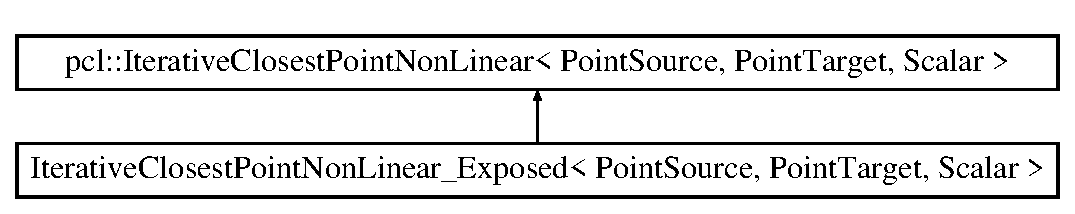
\includegraphics[height=2.000000cm]{classIterativeClosestPointNonLinear__Exposed}
\end{center}
\end{figure}
\subsection*{Public Member Functions}
\begin{DoxyCompactItemize}
\item 
pcl\-::\-Correspondences\-Ptr \hyperlink{classIterativeClosestPointNonLinear__Exposed_a8b5c6960d7914db1325d25e55d6d902b}{get\-Correspondences\-Ptr} ()
\end{DoxyCompactItemize}


\subsection{Detailed Description}
\subsubsection*{template$<$typename Point\-Source, typename Point\-Target, typename Scalar = float$>$class Iterative\-Closest\-Point\-Non\-Linear\-\_\-\-Exposed$<$ Point\-Source, Point\-Target, Scalar $>$}

This is a mock class with the sole purpose of accessing a protected member of a class it inherits from. 

Some of the relevant documentation\-: \href{http://docs.pointclouds.org/trunk/correspondence_8h_source.html#l00092}{\tt http\-://docs.\-pointclouds.\-org/trunk/correspondence\-\_\-8h\-\_\-source.\-html\#l00092} 

\subsection{Member Function Documentation}
\hypertarget{classIterativeClosestPointNonLinear__Exposed_a8b5c6960d7914db1325d25e55d6d902b}{\index{Iterative\-Closest\-Point\-Non\-Linear\-\_\-\-Exposed@{Iterative\-Closest\-Point\-Non\-Linear\-\_\-\-Exposed}!get\-Correspondences\-Ptr@{get\-Correspondences\-Ptr}}
\index{get\-Correspondences\-Ptr@{get\-Correspondences\-Ptr}!IterativeClosestPointNonLinear_Exposed@{Iterative\-Closest\-Point\-Non\-Linear\-\_\-\-Exposed}}
\subsubsection[{get\-Correspondences\-Ptr}]{\setlength{\rightskip}{0pt plus 5cm}template$<$typename Point\-Source , typename Point\-Target , typename Scalar  = float$>$ pcl\-::\-Correspondences\-Ptr {\bf Iterative\-Closest\-Point\-Non\-Linear\-\_\-\-Exposed}$<$ Point\-Source, Point\-Target, Scalar $>$\-::get\-Correspondences\-Ptr (
\begin{DoxyParamCaption}
{}
\end{DoxyParamCaption}
)\hspace{0.3cm}{\ttfamily [inline]}}}\label{classIterativeClosestPointNonLinear__Exposed_a8b5c6960d7914db1325d25e55d6d902b}


The documentation for this class was generated from the following file\-:\begin{DoxyCompactItemize}
\item 
\hyperlink{IterativeClosestPoint_8h}{Iterative\-Closest\-Point.\-h}\end{DoxyCompactItemize}

\hypertarget{classIterativeClosestPointParameters}{\section{Iterative\-Closest\-Point\-Parameters Class Reference}
\label{classIterativeClosestPointParameters}\index{Iterative\-Closest\-Point\-Parameters@{Iterative\-Closest\-Point\-Parameters}}
}


Parameters obtained from the input .xml file used to perform iterative closest point registration.  




{\ttfamily \#include $<$input\-Params.\-h$>$}

\subsection*{Public Member Functions}
\begin{DoxyCompactItemize}
\item 
\hyperlink{classIterativeClosestPointParameters_ac22cf5ddf2c6bdf35e4a25d520607c93}{Iterative\-Closest\-Point\-Parameters} ()
\item 
\hyperlink{classIterativeClosestPointParameters_a6bf05e4be2c1dacecaf5fcbf0e39c859}{$\sim$\-Iterative\-Closest\-Point\-Parameters} ()
\item 
int \hyperlink{classIterativeClosestPointParameters_a6f9644c27cf260b51875e648df2f5383}{get\-Maximum\-Iterations} ()
\item 
void \hyperlink{classIterativeClosestPointParameters_ab793da4dfd1166ed410a4ce75564fa42}{set\-Maximum\-Iterations} (int input\-Maximum\-Iterations)
\item 
float \hyperlink{classIterativeClosestPointParameters_a85b817764264f245084458c5b1d29495}{get\-Max\-Correspondence\-Distance} ()
\item 
void \hyperlink{classIterativeClosestPointParameters_ace991aa94a654839617451db83e7957c}{set\-Max\-Correspondence\-Distance} (float input\-Max\-Correspondence\-Distance)
\item 
float \hyperlink{classIterativeClosestPointParameters_a54bfe06276b42c30c4696260691baf88}{get\-Min\-Correspondence\-Distance} ()
\item 
void \hyperlink{classIterativeClosestPointParameters_a8b61a05336a7f00d91d7eb6a2774615a}{set\-Min\-Correspondence\-Distance} (float input\-Min\-Correspondence\-Distance)
\item 
float \hyperlink{classIterativeClosestPointParameters_ab7073c148fc7f27b6eefa9ad09c458fa}{get\-Large\-Correspondence\-Distance\-Step\-Reduction} ()
\item 
void \hyperlink{classIterativeClosestPointParameters_a58c4a6d6a2dfc4c5af3f25ae2c7b1887}{set\-Large\-Correspondence\-Distance\-Step\-Reduction} (float input\-Large\-Correspondence\-Distance\-Step\-Reduction)
\item 
float \hyperlink{classIterativeClosestPointParameters_a0d05c1de0da47367703f8f8ba7272fce}{get\-Small\-Correspondence\-Distance\-Step\-Reduction} ()
\item 
void \hyperlink{classIterativeClosestPointParameters_a2318311bbba1ebf252572ada4983ad58}{set\-Small\-Correspondence\-Distance\-Step\-Reduction} (float input\-Small\-Correspondence\-Distance\-Step\-Reduction)
\item 
float \hyperlink{classIterativeClosestPointParameters_a816c8ed3a323e3b1a38dd6ba09c38f85}{get\-Threshold\-Switch\-From\-Large\-To\-Small\-Distance\-Steps} ()
\item 
void \hyperlink{classIterativeClosestPointParameters_a05a1d4739cdf40be86004f92dbc16f32}{set\-Threshold\-Switch\-From\-Large\-To\-Small\-Distance\-Steps} (float input\-Threshold\-Switch\-From\-Large\-To\-Small\-Distance\-Steps)
\item 
float \hyperlink{classIterativeClosestPointParameters_a0e8f1f89a2612eea2617c3d60d7a7965}{get\-Fitness\-Threshold\-Defining\-Failure} ()
\item 
void \hyperlink{classIterativeClosestPointParameters_ab25b2e63147776c5d45a10f8505a22b4}{set\-Fitness\-Threshold\-Defining\-Failure} (float input\-Fitness\-Threshold\-Defining\-Failure)
\item 
void \hyperlink{classIterativeClosestPointParameters_a6e5267a21bd5949c6be2d522f92b3a98}{print\-Parameters} ()
\end{DoxyCompactItemize}
\subsection*{Private Attributes}
\begin{DoxyCompactItemize}
\item 
float \hyperlink{classIterativeClosestPointParameters_a8b9b3a2560aad7053b51838178a77448}{\-\_\-\-Maximum\-Iterations}
\item 
float \hyperlink{classIterativeClosestPointParameters_ad8339424eb93a8c4b21ded0bfc7e31db}{\-\_\-\-Max\-Correspondence\-Distance}
\item 
float \hyperlink{classIterativeClosestPointParameters_a0ac4b3b1537c98e6e4a0455db1965d5f}{\-\_\-\-Min\-Correspondence\-Distance}
\item 
float \hyperlink{classIterativeClosestPointParameters_a7e4ba577ce0925364c436defb7848f3e}{\-\_\-\-Large\-Correspondence\-Distance\-Step\-Reduction}
\item 
float \hyperlink{classIterativeClosestPointParameters_af7464d662390ed1a01d2208f6b615dc4}{\-\_\-\-Small\-Correspondence\-Distance\-Step\-Reduction}
\item 
float \hyperlink{classIterativeClosestPointParameters_a65c322e9bacd48481fb2bb9b49501893}{\-\_\-\-Threshold\-Switch\-From\-Large\-To\-Small\-Distance\-Steps}
\item 
float \hyperlink{classIterativeClosestPointParameters_abd7ebdbc7022d2fc7f321103139bb0d9}{\-\_\-\-Fitness\-Threshold\-Defining\-Failure}
\end{DoxyCompactItemize}


\subsection{Detailed Description}
Parameters obtained from the input .xml file used to perform iterative closest point registration. 

\subsection{Constructor \& Destructor Documentation}
\hypertarget{classIterativeClosestPointParameters_ac22cf5ddf2c6bdf35e4a25d520607c93}{\index{Iterative\-Closest\-Point\-Parameters@{Iterative\-Closest\-Point\-Parameters}!Iterative\-Closest\-Point\-Parameters@{Iterative\-Closest\-Point\-Parameters}}
\index{Iterative\-Closest\-Point\-Parameters@{Iterative\-Closest\-Point\-Parameters}!IterativeClosestPointParameters@{Iterative\-Closest\-Point\-Parameters}}
\subsubsection[{Iterative\-Closest\-Point\-Parameters}]{\setlength{\rightskip}{0pt plus 5cm}Iterative\-Closest\-Point\-Parameters\-::\-Iterative\-Closest\-Point\-Parameters (
\begin{DoxyParamCaption}
{}
\end{DoxyParamCaption}
)}}\label{classIterativeClosestPointParameters_ac22cf5ddf2c6bdf35e4a25d520607c93}
\hypertarget{classIterativeClosestPointParameters_a6bf05e4be2c1dacecaf5fcbf0e39c859}{\index{Iterative\-Closest\-Point\-Parameters@{Iterative\-Closest\-Point\-Parameters}!$\sim$\-Iterative\-Closest\-Point\-Parameters@{$\sim$\-Iterative\-Closest\-Point\-Parameters}}
\index{$\sim$\-Iterative\-Closest\-Point\-Parameters@{$\sim$\-Iterative\-Closest\-Point\-Parameters}!IterativeClosestPointParameters@{Iterative\-Closest\-Point\-Parameters}}
\subsubsection[{$\sim$\-Iterative\-Closest\-Point\-Parameters}]{\setlength{\rightskip}{0pt plus 5cm}Iterative\-Closest\-Point\-Parameters\-::$\sim$\-Iterative\-Closest\-Point\-Parameters (
\begin{DoxyParamCaption}
{}
\end{DoxyParamCaption}
)}}\label{classIterativeClosestPointParameters_a6bf05e4be2c1dacecaf5fcbf0e39c859}


\subsection{Member Function Documentation}
\hypertarget{classIterativeClosestPointParameters_a0e8f1f89a2612eea2617c3d60d7a7965}{\index{Iterative\-Closest\-Point\-Parameters@{Iterative\-Closest\-Point\-Parameters}!get\-Fitness\-Threshold\-Defining\-Failure@{get\-Fitness\-Threshold\-Defining\-Failure}}
\index{get\-Fitness\-Threshold\-Defining\-Failure@{get\-Fitness\-Threshold\-Defining\-Failure}!IterativeClosestPointParameters@{Iterative\-Closest\-Point\-Parameters}}
\subsubsection[{get\-Fitness\-Threshold\-Defining\-Failure}]{\setlength{\rightskip}{0pt plus 5cm}float Iterative\-Closest\-Point\-Parameters\-::get\-Fitness\-Threshold\-Defining\-Failure (
\begin{DoxyParamCaption}
{}
\end{DoxyParamCaption}
)}}\label{classIterativeClosestPointParameters_a0e8f1f89a2612eea2617c3d60d7a7965}
\hypertarget{classIterativeClosestPointParameters_ab7073c148fc7f27b6eefa9ad09c458fa}{\index{Iterative\-Closest\-Point\-Parameters@{Iterative\-Closest\-Point\-Parameters}!get\-Large\-Correspondence\-Distance\-Step\-Reduction@{get\-Large\-Correspondence\-Distance\-Step\-Reduction}}
\index{get\-Large\-Correspondence\-Distance\-Step\-Reduction@{get\-Large\-Correspondence\-Distance\-Step\-Reduction}!IterativeClosestPointParameters@{Iterative\-Closest\-Point\-Parameters}}
\subsubsection[{get\-Large\-Correspondence\-Distance\-Step\-Reduction}]{\setlength{\rightskip}{0pt plus 5cm}float Iterative\-Closest\-Point\-Parameters\-::get\-Large\-Correspondence\-Distance\-Step\-Reduction (
\begin{DoxyParamCaption}
{}
\end{DoxyParamCaption}
)}}\label{classIterativeClosestPointParameters_ab7073c148fc7f27b6eefa9ad09c458fa}
\hypertarget{classIterativeClosestPointParameters_a85b817764264f245084458c5b1d29495}{\index{Iterative\-Closest\-Point\-Parameters@{Iterative\-Closest\-Point\-Parameters}!get\-Max\-Correspondence\-Distance@{get\-Max\-Correspondence\-Distance}}
\index{get\-Max\-Correspondence\-Distance@{get\-Max\-Correspondence\-Distance}!IterativeClosestPointParameters@{Iterative\-Closest\-Point\-Parameters}}
\subsubsection[{get\-Max\-Correspondence\-Distance}]{\setlength{\rightskip}{0pt plus 5cm}float Iterative\-Closest\-Point\-Parameters\-::get\-Max\-Correspondence\-Distance (
\begin{DoxyParamCaption}
{}
\end{DoxyParamCaption}
)}}\label{classIterativeClosestPointParameters_a85b817764264f245084458c5b1d29495}
\hypertarget{classIterativeClosestPointParameters_a6f9644c27cf260b51875e648df2f5383}{\index{Iterative\-Closest\-Point\-Parameters@{Iterative\-Closest\-Point\-Parameters}!get\-Maximum\-Iterations@{get\-Maximum\-Iterations}}
\index{get\-Maximum\-Iterations@{get\-Maximum\-Iterations}!IterativeClosestPointParameters@{Iterative\-Closest\-Point\-Parameters}}
\subsubsection[{get\-Maximum\-Iterations}]{\setlength{\rightskip}{0pt plus 5cm}int Iterative\-Closest\-Point\-Parameters\-::get\-Maximum\-Iterations (
\begin{DoxyParamCaption}
{}
\end{DoxyParamCaption}
)}}\label{classIterativeClosestPointParameters_a6f9644c27cf260b51875e648df2f5383}
\hypertarget{classIterativeClosestPointParameters_a54bfe06276b42c30c4696260691baf88}{\index{Iterative\-Closest\-Point\-Parameters@{Iterative\-Closest\-Point\-Parameters}!get\-Min\-Correspondence\-Distance@{get\-Min\-Correspondence\-Distance}}
\index{get\-Min\-Correspondence\-Distance@{get\-Min\-Correspondence\-Distance}!IterativeClosestPointParameters@{Iterative\-Closest\-Point\-Parameters}}
\subsubsection[{get\-Min\-Correspondence\-Distance}]{\setlength{\rightskip}{0pt plus 5cm}float Iterative\-Closest\-Point\-Parameters\-::get\-Min\-Correspondence\-Distance (
\begin{DoxyParamCaption}
{}
\end{DoxyParamCaption}
)}}\label{classIterativeClosestPointParameters_a54bfe06276b42c30c4696260691baf88}
\hypertarget{classIterativeClosestPointParameters_a0d05c1de0da47367703f8f8ba7272fce}{\index{Iterative\-Closest\-Point\-Parameters@{Iterative\-Closest\-Point\-Parameters}!get\-Small\-Correspondence\-Distance\-Step\-Reduction@{get\-Small\-Correspondence\-Distance\-Step\-Reduction}}
\index{get\-Small\-Correspondence\-Distance\-Step\-Reduction@{get\-Small\-Correspondence\-Distance\-Step\-Reduction}!IterativeClosestPointParameters@{Iterative\-Closest\-Point\-Parameters}}
\subsubsection[{get\-Small\-Correspondence\-Distance\-Step\-Reduction}]{\setlength{\rightskip}{0pt plus 5cm}float Iterative\-Closest\-Point\-Parameters\-::get\-Small\-Correspondence\-Distance\-Step\-Reduction (
\begin{DoxyParamCaption}
{}
\end{DoxyParamCaption}
)}}\label{classIterativeClosestPointParameters_a0d05c1de0da47367703f8f8ba7272fce}
\hypertarget{classIterativeClosestPointParameters_a816c8ed3a323e3b1a38dd6ba09c38f85}{\index{Iterative\-Closest\-Point\-Parameters@{Iterative\-Closest\-Point\-Parameters}!get\-Threshold\-Switch\-From\-Large\-To\-Small\-Distance\-Steps@{get\-Threshold\-Switch\-From\-Large\-To\-Small\-Distance\-Steps}}
\index{get\-Threshold\-Switch\-From\-Large\-To\-Small\-Distance\-Steps@{get\-Threshold\-Switch\-From\-Large\-To\-Small\-Distance\-Steps}!IterativeClosestPointParameters@{Iterative\-Closest\-Point\-Parameters}}
\subsubsection[{get\-Threshold\-Switch\-From\-Large\-To\-Small\-Distance\-Steps}]{\setlength{\rightskip}{0pt plus 5cm}float Iterative\-Closest\-Point\-Parameters\-::get\-Threshold\-Switch\-From\-Large\-To\-Small\-Distance\-Steps (
\begin{DoxyParamCaption}
{}
\end{DoxyParamCaption}
)}}\label{classIterativeClosestPointParameters_a816c8ed3a323e3b1a38dd6ba09c38f85}
\hypertarget{classIterativeClosestPointParameters_a6e5267a21bd5949c6be2d522f92b3a98}{\index{Iterative\-Closest\-Point\-Parameters@{Iterative\-Closest\-Point\-Parameters}!print\-Parameters@{print\-Parameters}}
\index{print\-Parameters@{print\-Parameters}!IterativeClosestPointParameters@{Iterative\-Closest\-Point\-Parameters}}
\subsubsection[{print\-Parameters}]{\setlength{\rightskip}{0pt plus 5cm}void Iterative\-Closest\-Point\-Parameters\-::print\-Parameters (
\begin{DoxyParamCaption}
{}
\end{DoxyParamCaption}
)}}\label{classIterativeClosestPointParameters_a6e5267a21bd5949c6be2d522f92b3a98}
\hypertarget{classIterativeClosestPointParameters_ab25b2e63147776c5d45a10f8505a22b4}{\index{Iterative\-Closest\-Point\-Parameters@{Iterative\-Closest\-Point\-Parameters}!set\-Fitness\-Threshold\-Defining\-Failure@{set\-Fitness\-Threshold\-Defining\-Failure}}
\index{set\-Fitness\-Threshold\-Defining\-Failure@{set\-Fitness\-Threshold\-Defining\-Failure}!IterativeClosestPointParameters@{Iterative\-Closest\-Point\-Parameters}}
\subsubsection[{set\-Fitness\-Threshold\-Defining\-Failure}]{\setlength{\rightskip}{0pt plus 5cm}void Iterative\-Closest\-Point\-Parameters\-::set\-Fitness\-Threshold\-Defining\-Failure (
\begin{DoxyParamCaption}
\item[{float}]{input\-Fitness\-Threshold\-Defining\-Failure}
\end{DoxyParamCaption}
)}}\label{classIterativeClosestPointParameters_ab25b2e63147776c5d45a10f8505a22b4}
\hypertarget{classIterativeClosestPointParameters_a58c4a6d6a2dfc4c5af3f25ae2c7b1887}{\index{Iterative\-Closest\-Point\-Parameters@{Iterative\-Closest\-Point\-Parameters}!set\-Large\-Correspondence\-Distance\-Step\-Reduction@{set\-Large\-Correspondence\-Distance\-Step\-Reduction}}
\index{set\-Large\-Correspondence\-Distance\-Step\-Reduction@{set\-Large\-Correspondence\-Distance\-Step\-Reduction}!IterativeClosestPointParameters@{Iterative\-Closest\-Point\-Parameters}}
\subsubsection[{set\-Large\-Correspondence\-Distance\-Step\-Reduction}]{\setlength{\rightskip}{0pt plus 5cm}void Iterative\-Closest\-Point\-Parameters\-::set\-Large\-Correspondence\-Distance\-Step\-Reduction (
\begin{DoxyParamCaption}
\item[{float}]{input\-Large\-Correspondence\-Distance\-Step\-Reduction}
\end{DoxyParamCaption}
)}}\label{classIterativeClosestPointParameters_a58c4a6d6a2dfc4c5af3f25ae2c7b1887}
\hypertarget{classIterativeClosestPointParameters_ace991aa94a654839617451db83e7957c}{\index{Iterative\-Closest\-Point\-Parameters@{Iterative\-Closest\-Point\-Parameters}!set\-Max\-Correspondence\-Distance@{set\-Max\-Correspondence\-Distance}}
\index{set\-Max\-Correspondence\-Distance@{set\-Max\-Correspondence\-Distance}!IterativeClosestPointParameters@{Iterative\-Closest\-Point\-Parameters}}
\subsubsection[{set\-Max\-Correspondence\-Distance}]{\setlength{\rightskip}{0pt plus 5cm}void Iterative\-Closest\-Point\-Parameters\-::set\-Max\-Correspondence\-Distance (
\begin{DoxyParamCaption}
\item[{float}]{input\-Max\-Correspondence\-Distance}
\end{DoxyParamCaption}
)}}\label{classIterativeClosestPointParameters_ace991aa94a654839617451db83e7957c}
\hypertarget{classIterativeClosestPointParameters_ab793da4dfd1166ed410a4ce75564fa42}{\index{Iterative\-Closest\-Point\-Parameters@{Iterative\-Closest\-Point\-Parameters}!set\-Maximum\-Iterations@{set\-Maximum\-Iterations}}
\index{set\-Maximum\-Iterations@{set\-Maximum\-Iterations}!IterativeClosestPointParameters@{Iterative\-Closest\-Point\-Parameters}}
\subsubsection[{set\-Maximum\-Iterations}]{\setlength{\rightskip}{0pt plus 5cm}void Iterative\-Closest\-Point\-Parameters\-::set\-Maximum\-Iterations (
\begin{DoxyParamCaption}
\item[{int}]{input\-Maximum\-Iterations}
\end{DoxyParamCaption}
)}}\label{classIterativeClosestPointParameters_ab793da4dfd1166ed410a4ce75564fa42}
\hypertarget{classIterativeClosestPointParameters_a8b61a05336a7f00d91d7eb6a2774615a}{\index{Iterative\-Closest\-Point\-Parameters@{Iterative\-Closest\-Point\-Parameters}!set\-Min\-Correspondence\-Distance@{set\-Min\-Correspondence\-Distance}}
\index{set\-Min\-Correspondence\-Distance@{set\-Min\-Correspondence\-Distance}!IterativeClosestPointParameters@{Iterative\-Closest\-Point\-Parameters}}
\subsubsection[{set\-Min\-Correspondence\-Distance}]{\setlength{\rightskip}{0pt plus 5cm}void Iterative\-Closest\-Point\-Parameters\-::set\-Min\-Correspondence\-Distance (
\begin{DoxyParamCaption}
\item[{float}]{input\-Min\-Correspondence\-Distance}
\end{DoxyParamCaption}
)}}\label{classIterativeClosestPointParameters_a8b61a05336a7f00d91d7eb6a2774615a}
\hypertarget{classIterativeClosestPointParameters_a2318311bbba1ebf252572ada4983ad58}{\index{Iterative\-Closest\-Point\-Parameters@{Iterative\-Closest\-Point\-Parameters}!set\-Small\-Correspondence\-Distance\-Step\-Reduction@{set\-Small\-Correspondence\-Distance\-Step\-Reduction}}
\index{set\-Small\-Correspondence\-Distance\-Step\-Reduction@{set\-Small\-Correspondence\-Distance\-Step\-Reduction}!IterativeClosestPointParameters@{Iterative\-Closest\-Point\-Parameters}}
\subsubsection[{set\-Small\-Correspondence\-Distance\-Step\-Reduction}]{\setlength{\rightskip}{0pt plus 5cm}void Iterative\-Closest\-Point\-Parameters\-::set\-Small\-Correspondence\-Distance\-Step\-Reduction (
\begin{DoxyParamCaption}
\item[{float}]{input\-Small\-Correspondence\-Distance\-Step\-Reduction}
\end{DoxyParamCaption}
)}}\label{classIterativeClosestPointParameters_a2318311bbba1ebf252572ada4983ad58}
\hypertarget{classIterativeClosestPointParameters_a05a1d4739cdf40be86004f92dbc16f32}{\index{Iterative\-Closest\-Point\-Parameters@{Iterative\-Closest\-Point\-Parameters}!set\-Threshold\-Switch\-From\-Large\-To\-Small\-Distance\-Steps@{set\-Threshold\-Switch\-From\-Large\-To\-Small\-Distance\-Steps}}
\index{set\-Threshold\-Switch\-From\-Large\-To\-Small\-Distance\-Steps@{set\-Threshold\-Switch\-From\-Large\-To\-Small\-Distance\-Steps}!IterativeClosestPointParameters@{Iterative\-Closest\-Point\-Parameters}}
\subsubsection[{set\-Threshold\-Switch\-From\-Large\-To\-Small\-Distance\-Steps}]{\setlength{\rightskip}{0pt plus 5cm}void Iterative\-Closest\-Point\-Parameters\-::set\-Threshold\-Switch\-From\-Large\-To\-Small\-Distance\-Steps (
\begin{DoxyParamCaption}
\item[{float}]{input\-Threshold\-Switch\-From\-Large\-To\-Small\-Distance\-Steps}
\end{DoxyParamCaption}
)}}\label{classIterativeClosestPointParameters_a05a1d4739cdf40be86004f92dbc16f32}


\subsection{Member Data Documentation}
\hypertarget{classIterativeClosestPointParameters_abd7ebdbc7022d2fc7f321103139bb0d9}{\index{Iterative\-Closest\-Point\-Parameters@{Iterative\-Closest\-Point\-Parameters}!\-\_\-\-Fitness\-Threshold\-Defining\-Failure@{\-\_\-\-Fitness\-Threshold\-Defining\-Failure}}
\index{\-\_\-\-Fitness\-Threshold\-Defining\-Failure@{\-\_\-\-Fitness\-Threshold\-Defining\-Failure}!IterativeClosestPointParameters@{Iterative\-Closest\-Point\-Parameters}}
\subsubsection[{\-\_\-\-Fitness\-Threshold\-Defining\-Failure}]{\setlength{\rightskip}{0pt plus 5cm}float Iterative\-Closest\-Point\-Parameters\-::\-\_\-\-Fitness\-Threshold\-Defining\-Failure\hspace{0.3cm}{\ttfamily [private]}}}\label{classIterativeClosestPointParameters_abd7ebdbc7022d2fc7f321103139bb0d9}
\hypertarget{classIterativeClosestPointParameters_a7e4ba577ce0925364c436defb7848f3e}{\index{Iterative\-Closest\-Point\-Parameters@{Iterative\-Closest\-Point\-Parameters}!\-\_\-\-Large\-Correspondence\-Distance\-Step\-Reduction@{\-\_\-\-Large\-Correspondence\-Distance\-Step\-Reduction}}
\index{\-\_\-\-Large\-Correspondence\-Distance\-Step\-Reduction@{\-\_\-\-Large\-Correspondence\-Distance\-Step\-Reduction}!IterativeClosestPointParameters@{Iterative\-Closest\-Point\-Parameters}}
\subsubsection[{\-\_\-\-Large\-Correspondence\-Distance\-Step\-Reduction}]{\setlength{\rightskip}{0pt plus 5cm}float Iterative\-Closest\-Point\-Parameters\-::\-\_\-\-Large\-Correspondence\-Distance\-Step\-Reduction\hspace{0.3cm}{\ttfamily [private]}}}\label{classIterativeClosestPointParameters_a7e4ba577ce0925364c436defb7848f3e}
\hypertarget{classIterativeClosestPointParameters_ad8339424eb93a8c4b21ded0bfc7e31db}{\index{Iterative\-Closest\-Point\-Parameters@{Iterative\-Closest\-Point\-Parameters}!\-\_\-\-Max\-Correspondence\-Distance@{\-\_\-\-Max\-Correspondence\-Distance}}
\index{\-\_\-\-Max\-Correspondence\-Distance@{\-\_\-\-Max\-Correspondence\-Distance}!IterativeClosestPointParameters@{Iterative\-Closest\-Point\-Parameters}}
\subsubsection[{\-\_\-\-Max\-Correspondence\-Distance}]{\setlength{\rightskip}{0pt plus 5cm}float Iterative\-Closest\-Point\-Parameters\-::\-\_\-\-Max\-Correspondence\-Distance\hspace{0.3cm}{\ttfamily [private]}}}\label{classIterativeClosestPointParameters_ad8339424eb93a8c4b21ded0bfc7e31db}
\hypertarget{classIterativeClosestPointParameters_a8b9b3a2560aad7053b51838178a77448}{\index{Iterative\-Closest\-Point\-Parameters@{Iterative\-Closest\-Point\-Parameters}!\-\_\-\-Maximum\-Iterations@{\-\_\-\-Maximum\-Iterations}}
\index{\-\_\-\-Maximum\-Iterations@{\-\_\-\-Maximum\-Iterations}!IterativeClosestPointParameters@{Iterative\-Closest\-Point\-Parameters}}
\subsubsection[{\-\_\-\-Maximum\-Iterations}]{\setlength{\rightskip}{0pt plus 5cm}float Iterative\-Closest\-Point\-Parameters\-::\-\_\-\-Maximum\-Iterations\hspace{0.3cm}{\ttfamily [private]}}}\label{classIterativeClosestPointParameters_a8b9b3a2560aad7053b51838178a77448}
\hypertarget{classIterativeClosestPointParameters_a0ac4b3b1537c98e6e4a0455db1965d5f}{\index{Iterative\-Closest\-Point\-Parameters@{Iterative\-Closest\-Point\-Parameters}!\-\_\-\-Min\-Correspondence\-Distance@{\-\_\-\-Min\-Correspondence\-Distance}}
\index{\-\_\-\-Min\-Correspondence\-Distance@{\-\_\-\-Min\-Correspondence\-Distance}!IterativeClosestPointParameters@{Iterative\-Closest\-Point\-Parameters}}
\subsubsection[{\-\_\-\-Min\-Correspondence\-Distance}]{\setlength{\rightskip}{0pt plus 5cm}float Iterative\-Closest\-Point\-Parameters\-::\-\_\-\-Min\-Correspondence\-Distance\hspace{0.3cm}{\ttfamily [private]}}}\label{classIterativeClosestPointParameters_a0ac4b3b1537c98e6e4a0455db1965d5f}
\hypertarget{classIterativeClosestPointParameters_af7464d662390ed1a01d2208f6b615dc4}{\index{Iterative\-Closest\-Point\-Parameters@{Iterative\-Closest\-Point\-Parameters}!\-\_\-\-Small\-Correspondence\-Distance\-Step\-Reduction@{\-\_\-\-Small\-Correspondence\-Distance\-Step\-Reduction}}
\index{\-\_\-\-Small\-Correspondence\-Distance\-Step\-Reduction@{\-\_\-\-Small\-Correspondence\-Distance\-Step\-Reduction}!IterativeClosestPointParameters@{Iterative\-Closest\-Point\-Parameters}}
\subsubsection[{\-\_\-\-Small\-Correspondence\-Distance\-Step\-Reduction}]{\setlength{\rightskip}{0pt plus 5cm}float Iterative\-Closest\-Point\-Parameters\-::\-\_\-\-Small\-Correspondence\-Distance\-Step\-Reduction\hspace{0.3cm}{\ttfamily [private]}}}\label{classIterativeClosestPointParameters_af7464d662390ed1a01d2208f6b615dc4}
\hypertarget{classIterativeClosestPointParameters_a65c322e9bacd48481fb2bb9b49501893}{\index{Iterative\-Closest\-Point\-Parameters@{Iterative\-Closest\-Point\-Parameters}!\-\_\-\-Threshold\-Switch\-From\-Large\-To\-Small\-Distance\-Steps@{\-\_\-\-Threshold\-Switch\-From\-Large\-To\-Small\-Distance\-Steps}}
\index{\-\_\-\-Threshold\-Switch\-From\-Large\-To\-Small\-Distance\-Steps@{\-\_\-\-Threshold\-Switch\-From\-Large\-To\-Small\-Distance\-Steps}!IterativeClosestPointParameters@{Iterative\-Closest\-Point\-Parameters}}
\subsubsection[{\-\_\-\-Threshold\-Switch\-From\-Large\-To\-Small\-Distance\-Steps}]{\setlength{\rightskip}{0pt plus 5cm}float Iterative\-Closest\-Point\-Parameters\-::\-\_\-\-Threshold\-Switch\-From\-Large\-To\-Small\-Distance\-Steps\hspace{0.3cm}{\ttfamily [private]}}}\label{classIterativeClosestPointParameters_a65c322e9bacd48481fb2bb9b49501893}


The documentation for this class was generated from the following files\-:\begin{DoxyCompactItemize}
\item 
\hyperlink{inputParams_8h}{input\-Params.\-h}\item 
\hyperlink{inputParams_8cpp}{input\-Params.\-cpp}\end{DoxyCompactItemize}

\hypertarget{classLSystemFitnessResults}{\section{L\-System\-Fitness\-Results Class Reference}
\label{classLSystemFitnessResults}\index{L\-System\-Fitness\-Results@{L\-System\-Fitness\-Results}}
}
\subsection*{Public Attributes}
\begin{DoxyCompactItemize}
\item 
float \hyperlink{classLSystemFitnessResults_a8a504f7f78aa6021eb3572668eb5dfba}{registration\-Fitness}
\item 
int \hyperlink{classLSystemFitnessResults_a5cf08d744b4f638cee64d7aeb8821c9c}{number\-Points\-Of\-Input\-Cloud\-Accounted\-For}
\item 
int \hyperlink{classLSystemFitnessResults_ae8d95ced155f6ac36e4eb19725cfe441}{number\-Points\-Of\-Input\-Cloud\-Unaccounted\-For}
\item 
float \hyperlink{classLSystemFitnessResults_aabc87d6a999ae7fa104048005c8bb1db}{proportion\-Of\-Input\-Cloud\-Accounted}
\item 
int \hyperlink{classLSystemFitnessResults_a1b5d9c64670dc73b4b075af30e1583bc}{number\-Points\-Of\-L\-System\-Cloud\-Accounted}
\item 
int \hyperlink{classLSystemFitnessResults_a9050be03d7e06c7a3d47b054b2326a9f}{number\-Points\-Of\-L\-System\-Cloud\-Unaccounted}
\item 
float \hyperlink{classLSystemFitnessResults_a814c4e058e6a642f60bc675303f1b491}{proportion\-Of\-L\-System\-Cloud\-Unaccounted}
\item 
float \hyperlink{classLSystemFitnessResults_af87917318b623a6624c91fb5ef587578}{combined\-Proportion\-Score}
\end{DoxyCompactItemize}


\subsection{Member Data Documentation}
\hypertarget{classLSystemFitnessResults_af87917318b623a6624c91fb5ef587578}{\index{L\-System\-Fitness\-Results@{L\-System\-Fitness\-Results}!combined\-Proportion\-Score@{combined\-Proportion\-Score}}
\index{combined\-Proportion\-Score@{combined\-Proportion\-Score}!LSystemFitnessResults@{L\-System\-Fitness\-Results}}
\subsubsection[{combined\-Proportion\-Score}]{\setlength{\rightskip}{0pt plus 5cm}float L\-System\-Fitness\-Results\-::combined\-Proportion\-Score}}\label{classLSystemFitnessResults_af87917318b623a6624c91fb5ef587578}
\hypertarget{classLSystemFitnessResults_a5cf08d744b4f638cee64d7aeb8821c9c}{\index{L\-System\-Fitness\-Results@{L\-System\-Fitness\-Results}!number\-Points\-Of\-Input\-Cloud\-Accounted\-For@{number\-Points\-Of\-Input\-Cloud\-Accounted\-For}}
\index{number\-Points\-Of\-Input\-Cloud\-Accounted\-For@{number\-Points\-Of\-Input\-Cloud\-Accounted\-For}!LSystemFitnessResults@{L\-System\-Fitness\-Results}}
\subsubsection[{number\-Points\-Of\-Input\-Cloud\-Accounted\-For}]{\setlength{\rightskip}{0pt plus 5cm}int L\-System\-Fitness\-Results\-::number\-Points\-Of\-Input\-Cloud\-Accounted\-For}}\label{classLSystemFitnessResults_a5cf08d744b4f638cee64d7aeb8821c9c}
\hypertarget{classLSystemFitnessResults_ae8d95ced155f6ac36e4eb19725cfe441}{\index{L\-System\-Fitness\-Results@{L\-System\-Fitness\-Results}!number\-Points\-Of\-Input\-Cloud\-Unaccounted\-For@{number\-Points\-Of\-Input\-Cloud\-Unaccounted\-For}}
\index{number\-Points\-Of\-Input\-Cloud\-Unaccounted\-For@{number\-Points\-Of\-Input\-Cloud\-Unaccounted\-For}!LSystemFitnessResults@{L\-System\-Fitness\-Results}}
\subsubsection[{number\-Points\-Of\-Input\-Cloud\-Unaccounted\-For}]{\setlength{\rightskip}{0pt plus 5cm}int L\-System\-Fitness\-Results\-::number\-Points\-Of\-Input\-Cloud\-Unaccounted\-For}}\label{classLSystemFitnessResults_ae8d95ced155f6ac36e4eb19725cfe441}
\hypertarget{classLSystemFitnessResults_a1b5d9c64670dc73b4b075af30e1583bc}{\index{L\-System\-Fitness\-Results@{L\-System\-Fitness\-Results}!number\-Points\-Of\-L\-System\-Cloud\-Accounted@{number\-Points\-Of\-L\-System\-Cloud\-Accounted}}
\index{number\-Points\-Of\-L\-System\-Cloud\-Accounted@{number\-Points\-Of\-L\-System\-Cloud\-Accounted}!LSystemFitnessResults@{L\-System\-Fitness\-Results}}
\subsubsection[{number\-Points\-Of\-L\-System\-Cloud\-Accounted}]{\setlength{\rightskip}{0pt plus 5cm}int L\-System\-Fitness\-Results\-::number\-Points\-Of\-L\-System\-Cloud\-Accounted}}\label{classLSystemFitnessResults_a1b5d9c64670dc73b4b075af30e1583bc}
\hypertarget{classLSystemFitnessResults_a9050be03d7e06c7a3d47b054b2326a9f}{\index{L\-System\-Fitness\-Results@{L\-System\-Fitness\-Results}!number\-Points\-Of\-L\-System\-Cloud\-Unaccounted@{number\-Points\-Of\-L\-System\-Cloud\-Unaccounted}}
\index{number\-Points\-Of\-L\-System\-Cloud\-Unaccounted@{number\-Points\-Of\-L\-System\-Cloud\-Unaccounted}!LSystemFitnessResults@{L\-System\-Fitness\-Results}}
\subsubsection[{number\-Points\-Of\-L\-System\-Cloud\-Unaccounted}]{\setlength{\rightskip}{0pt plus 5cm}int L\-System\-Fitness\-Results\-::number\-Points\-Of\-L\-System\-Cloud\-Unaccounted}}\label{classLSystemFitnessResults_a9050be03d7e06c7a3d47b054b2326a9f}
\hypertarget{classLSystemFitnessResults_aabc87d6a999ae7fa104048005c8bb1db}{\index{L\-System\-Fitness\-Results@{L\-System\-Fitness\-Results}!proportion\-Of\-Input\-Cloud\-Accounted@{proportion\-Of\-Input\-Cloud\-Accounted}}
\index{proportion\-Of\-Input\-Cloud\-Accounted@{proportion\-Of\-Input\-Cloud\-Accounted}!LSystemFitnessResults@{L\-System\-Fitness\-Results}}
\subsubsection[{proportion\-Of\-Input\-Cloud\-Accounted}]{\setlength{\rightskip}{0pt plus 5cm}float L\-System\-Fitness\-Results\-::proportion\-Of\-Input\-Cloud\-Accounted}}\label{classLSystemFitnessResults_aabc87d6a999ae7fa104048005c8bb1db}
\hypertarget{classLSystemFitnessResults_a814c4e058e6a642f60bc675303f1b491}{\index{L\-System\-Fitness\-Results@{L\-System\-Fitness\-Results}!proportion\-Of\-L\-System\-Cloud\-Unaccounted@{proportion\-Of\-L\-System\-Cloud\-Unaccounted}}
\index{proportion\-Of\-L\-System\-Cloud\-Unaccounted@{proportion\-Of\-L\-System\-Cloud\-Unaccounted}!LSystemFitnessResults@{L\-System\-Fitness\-Results}}
\subsubsection[{proportion\-Of\-L\-System\-Cloud\-Unaccounted}]{\setlength{\rightskip}{0pt plus 5cm}float L\-System\-Fitness\-Results\-::proportion\-Of\-L\-System\-Cloud\-Unaccounted}}\label{classLSystemFitnessResults_a814c4e058e6a642f60bc675303f1b491}
\hypertarget{classLSystemFitnessResults_a8a504f7f78aa6021eb3572668eb5dfba}{\index{L\-System\-Fitness\-Results@{L\-System\-Fitness\-Results}!registration\-Fitness@{registration\-Fitness}}
\index{registration\-Fitness@{registration\-Fitness}!LSystemFitnessResults@{L\-System\-Fitness\-Results}}
\subsubsection[{registration\-Fitness}]{\setlength{\rightskip}{0pt plus 5cm}float L\-System\-Fitness\-Results\-::registration\-Fitness}}\label{classLSystemFitnessResults_a8a504f7f78aa6021eb3572668eb5dfba}


The documentation for this class was generated from the following file\-:\begin{DoxyCompactItemize}
\item 
\hyperlink{lsystemRefinement_8cpp}{lsystem\-Refinement.\-cpp}\end{DoxyCompactItemize}

\hypertarget{classLSystemParameters}{\section{L\-System\-Parameters Class Reference}
\label{classLSystemParameters}\index{L\-System\-Parameters@{L\-System\-Parameters}}
}


{\ttfamily \#include $<$lsystem\-Parameters.\-h$>$}

\subsection*{Public Member Functions}
\begin{DoxyCompactItemize}
\item 
\hyperlink{classLSystemParameters_a23ecf893047602d4076b70d46e3d13f1}{L\-System\-Parameters} ()
\item 
\hyperlink{classLSystemParameters_a0cccedff9fc2f0ea82a5f3a89106a6de}{$\sim$\-L\-System\-Parameters} ()
\item 
void \hyperlink{classLSystemParameters_a14e47fea48f4d73bd363e86bc9ae8f85}{set\-Number\-Derivations} (int input\-Number\-Derivations)
\item 
int \hyperlink{classLSystemParameters_a922f8a577c222df6330735bc6f9dd847}{get\-Number\-Derivations} ()
\item 
void \hyperlink{classLSystemParameters_ac2d66eb83df0a7569285c77777b59555}{set\-Internode\-Lengths} (std\-::vector$<$ float $>$ input\-Internode\-Lengths)
\item 
void \hyperlink{classLSystemParameters_aa3b4318d190e105b629225eaa624efc8}{append\-Internode\-Length} (float input\-Internode\-Length)
\item 
std\-::vector$<$ float $>$ \hyperlink{classLSystemParameters_af91d7c9254210830a3c7ead31c54cae9}{get\-Internode\-Lengths} ()
\item 
void \hyperlink{classLSystemParameters_ae602c3d680038b52145d2e9c57f10900}{set\-Internode\-Radii} (std\-::vector$<$ float $>$ input\-Internode\-Radii)
\item 
void \hyperlink{classLSystemParameters_a1a91050d244b8f758ae67f1d75afcaa2}{append\-Internode\-Radius} (float input\-Internode\-Radius)
\item 
std\-::vector$<$ float $>$ \hyperlink{classLSystemParameters_ad74efb57707873999645bf4b542d1f18}{get\-Internode\-Radii} ()
\item 
void \hyperlink{classLSystemParameters_a9e0f7914e97c1998009ef34d15e23025}{set\-Internode\-Pitch\-Angles} (std\-::vector$<$ float $>$ input\-Pitch\-Angles)
\begin{DoxyCompactList}\small\item\em Pitches up by angle around the L axis (seems to be Y). Corresponds to \char`\"{}$^\wedge$\char`\"{} instruction.$>$ \end{DoxyCompactList}\item 
void \hyperlink{classLSystemParameters_af605476ba5e0315e53617953eda145ec}{append\-Internode\-Pitch\-Angle} (float input\-Pitch\-Angle)
\item 
std\-::vector$<$ float $>$ \hyperlink{classLSystemParameters_a25f10717a3d2ffb4caa6949e67b05170}{get\-Internode\-Pitch\-Angles} ()
\begin{DoxyCompactList}\small\item\em Pitches up by angle around the L axis (seems to be Y). Corresponds to \char`\"{}$^\wedge$\char`\"{} instruction. $>$ \end{DoxyCompactList}\item 
void \hyperlink{classLSystemParameters_a11964e14c43fb1dbd443006173ac3993}{set\-Internode\-Turn\-Angles} (std\-::vector$<$ float $>$ input\-Turn\-Angles)
\begin{DoxyCompactList}\small\item\em Turns right by angle around the U axis (seems to be X). Corresponds to \char`\"{}-\/\char`\"{} instruction. $>$ \end{DoxyCompactList}\item 
void \hyperlink{classLSystemParameters_a42c09989d87627bfd5217d5799de6261}{append\-Internode\-Turn\-Angle} (float input\-Turn\-Angle)
\item 
std\-::vector$<$ float $>$ \hyperlink{classLSystemParameters_ae75f4c86bceacdd960c3a41a2de94265}{get\-Internode\-Turn\-Angles} ()
\begin{DoxyCompactList}\small\item\em Turns right by angle around the U axis (seems to be X). Corresponds to \char`\"{}-\/\char`\"{} instruction. $>$ \end{DoxyCompactList}\item 
void \hyperlink{classLSystemParameters_aac5a310edc93f3f431d0bbcef0f64bb5}{set\-Leaf\-Phyllotaxy\-Angles} (std\-::vector$<$ float $>$ input\-Leaf\-Phyllotaxy\-Angles)
\begin{DoxyCompactList}\small\item\em Turns counter-\/clockwise around Z axis, starting along X axis. Corresponds to \char`\"{}/\char`\"{} instruction. $>$ \end{DoxyCompactList}\item 
void \hyperlink{classLSystemParameters_abfe638849fd39e447a12231b1ca22a50}{append\-Leaf\-Phyllotaxy\-Angle} (float input\-Leaf\-Phyllotaxy\-Angle)
\item 
std\-::vector$<$ float $>$ \hyperlink{classLSystemParameters_ad28db9029a6879362cd7af7f969c3f87}{get\-Leaf\-Phyllotaxy\-Angles} ()
\begin{DoxyCompactList}\small\item\em Turns counter-\/clockwise around Z axis, starting along X axis. Corresponds to \char`\"{}/\char`\"{} instruction. $>$ \end{DoxyCompactList}\item 
void \hyperlink{classLSystemParameters_a8518e051415f3684548081ebe4e6d079}{set\-Leaf\-Widths} (std\-::vector$<$ float $>$ input\-Leaf\-Widths)
\item 
void \hyperlink{classLSystemParameters_a5ba39d60b7c69f087292d1a69468611f}{append\-Leaf\-Width} (float input\-Leaf\-Width)
\item 
std\-::vector$<$ float $>$ \hyperlink{classLSystemParameters_ae8236379ad72509c59c784f08d9a752b}{get\-Leaf\-Widths} ()
\item 
void \hyperlink{classLSystemParameters_a1dc078c5bc7d25a951c523bd8bbd16db}{set\-Leaf\-Curvatures} (std\-::vector$<$ std\-::vector$<$ std\-::pair$<$ float, float $>$ $>$ $>$ input\-Leaf\-Curvatures)
\item 
void \hyperlink{classLSystemParameters_a3db8d293bc9d8a7d50f93202f88be317}{append\-Leaf\-Curvature} (std\-::vector$<$ std\-::pair$<$ float, float $>$ $>$ input\-Leaf\-Curvature)
\item 
std\-::vector$<$ std\-::vector\\*
$<$ std\-::pair$<$ float, float $>$ $>$ $>$ \hyperlink{classLSystemParameters_a127b9e85d7d1f6071f720709d324be88}{get\-Leaf\-Curvatures} ()
\end{DoxyCompactItemize}
\subsection*{Private Attributes}
\begin{DoxyCompactItemize}
\item 
int \hyperlink{classLSystemParameters_aa6c15efa6da78e759317beebcd63072d}{\-\_\-number\-Derivations}
\item 
std\-::vector$<$ float $>$ \hyperlink{classLSystemParameters_a2465e8385f6f4a44e6066b8e373f911a}{\-\_\-internode\-Lengths}
\item 
std\-::vector$<$ float $>$ \hyperlink{classLSystemParameters_aed5693a39acfe7da5f2338a470fa56da}{\-\_\-internode\-Radii}
\item 
std\-::vector$<$ float $>$ \hyperlink{classLSystemParameters_a262a0b893a9ef18489b35cce0b6053b6}{\-\_\-internode\-Pitch\-Angles}
\begin{DoxyCompactList}\small\item\em Pitches up by angle around the L axis (seems to be Y). Corresponds to \char`\"{}$^\wedge$\char`\"{} instruction. $>$ \end{DoxyCompactList}\item 
std\-::vector$<$ float $>$ \hyperlink{classLSystemParameters_af078859120313ef883b1ac15dddc8330}{\-\_\-internode\-Turn\-Angles}
\begin{DoxyCompactList}\small\item\em Turns right by angle around the U axis (seems to be X). Corresponds to \char`\"{}-\/\char`\"{} instruction. $>$ \end{DoxyCompactList}\item 
std\-::vector$<$ float $>$ \hyperlink{classLSystemParameters_ad34438ab953227fe2810433f2c0fbcd6}{\-\_\-leaf\-Phyllotaxy\-Angles}
\begin{DoxyCompactList}\small\item\em Turns counter-\/clockwise around Z axis, starting along X axis. Corresponds to \char`\"{}/\char`\"{} instruction. $>$ \end{DoxyCompactList}\item 
std\-::vector$<$ float $>$ \hyperlink{classLSystemParameters_afdad1e5edf4a2d3f00012f0ad8d5d6f3}{\-\_\-leaf\-Widths}
\item 
std\-::vector$<$ std\-::vector\\*
$<$ std\-::pair$<$ float, float $>$ $>$ $>$ \hyperlink{classLSystemParameters_a257d10b96cb874d2756013098f8c7095}{\-\_\-leaf\-Curvatures}
\end{DoxyCompactItemize}


\subsection{Constructor \& Destructor Documentation}
\hypertarget{classLSystemParameters_a23ecf893047602d4076b70d46e3d13f1}{\index{L\-System\-Parameters@{L\-System\-Parameters}!L\-System\-Parameters@{L\-System\-Parameters}}
\index{L\-System\-Parameters@{L\-System\-Parameters}!LSystemParameters@{L\-System\-Parameters}}
\subsubsection[{L\-System\-Parameters}]{\setlength{\rightskip}{0pt plus 5cm}L\-System\-Parameters\-::\-L\-System\-Parameters (
\begin{DoxyParamCaption}
{}
\end{DoxyParamCaption}
)}}\label{classLSystemParameters_a23ecf893047602d4076b70d46e3d13f1}
\hypertarget{classLSystemParameters_a0cccedff9fc2f0ea82a5f3a89106a6de}{\index{L\-System\-Parameters@{L\-System\-Parameters}!$\sim$\-L\-System\-Parameters@{$\sim$\-L\-System\-Parameters}}
\index{$\sim$\-L\-System\-Parameters@{$\sim$\-L\-System\-Parameters}!LSystemParameters@{L\-System\-Parameters}}
\subsubsection[{$\sim$\-L\-System\-Parameters}]{\setlength{\rightskip}{0pt plus 5cm}L\-System\-Parameters\-::$\sim$\-L\-System\-Parameters (
\begin{DoxyParamCaption}
{}
\end{DoxyParamCaption}
)}}\label{classLSystemParameters_a0cccedff9fc2f0ea82a5f3a89106a6de}


\subsection{Member Function Documentation}
\hypertarget{classLSystemParameters_aa3b4318d190e105b629225eaa624efc8}{\index{L\-System\-Parameters@{L\-System\-Parameters}!append\-Internode\-Length@{append\-Internode\-Length}}
\index{append\-Internode\-Length@{append\-Internode\-Length}!LSystemParameters@{L\-System\-Parameters}}
\subsubsection[{append\-Internode\-Length}]{\setlength{\rightskip}{0pt plus 5cm}void L\-System\-Parameters\-::append\-Internode\-Length (
\begin{DoxyParamCaption}
\item[{float}]{input\-Internode\-Length}
\end{DoxyParamCaption}
)}}\label{classLSystemParameters_aa3b4318d190e105b629225eaa624efc8}
\hypertarget{classLSystemParameters_af605476ba5e0315e53617953eda145ec}{\index{L\-System\-Parameters@{L\-System\-Parameters}!append\-Internode\-Pitch\-Angle@{append\-Internode\-Pitch\-Angle}}
\index{append\-Internode\-Pitch\-Angle@{append\-Internode\-Pitch\-Angle}!LSystemParameters@{L\-System\-Parameters}}
\subsubsection[{append\-Internode\-Pitch\-Angle}]{\setlength{\rightskip}{0pt plus 5cm}void L\-System\-Parameters\-::append\-Internode\-Pitch\-Angle (
\begin{DoxyParamCaption}
\item[{float}]{input\-Pitch\-Angle}
\end{DoxyParamCaption}
)}}\label{classLSystemParameters_af605476ba5e0315e53617953eda145ec}
\hypertarget{classLSystemParameters_a1a91050d244b8f758ae67f1d75afcaa2}{\index{L\-System\-Parameters@{L\-System\-Parameters}!append\-Internode\-Radius@{append\-Internode\-Radius}}
\index{append\-Internode\-Radius@{append\-Internode\-Radius}!LSystemParameters@{L\-System\-Parameters}}
\subsubsection[{append\-Internode\-Radius}]{\setlength{\rightskip}{0pt plus 5cm}void L\-System\-Parameters\-::append\-Internode\-Radius (
\begin{DoxyParamCaption}
\item[{float}]{input\-Internode\-Radius}
\end{DoxyParamCaption}
)}}\label{classLSystemParameters_a1a91050d244b8f758ae67f1d75afcaa2}
\hypertarget{classLSystemParameters_a42c09989d87627bfd5217d5799de6261}{\index{L\-System\-Parameters@{L\-System\-Parameters}!append\-Internode\-Turn\-Angle@{append\-Internode\-Turn\-Angle}}
\index{append\-Internode\-Turn\-Angle@{append\-Internode\-Turn\-Angle}!LSystemParameters@{L\-System\-Parameters}}
\subsubsection[{append\-Internode\-Turn\-Angle}]{\setlength{\rightskip}{0pt plus 5cm}void L\-System\-Parameters\-::append\-Internode\-Turn\-Angle (
\begin{DoxyParamCaption}
\item[{float}]{input\-Turn\-Angle}
\end{DoxyParamCaption}
)}}\label{classLSystemParameters_a42c09989d87627bfd5217d5799de6261}
\hypertarget{classLSystemParameters_a3db8d293bc9d8a7d50f93202f88be317}{\index{L\-System\-Parameters@{L\-System\-Parameters}!append\-Leaf\-Curvature@{append\-Leaf\-Curvature}}
\index{append\-Leaf\-Curvature@{append\-Leaf\-Curvature}!LSystemParameters@{L\-System\-Parameters}}
\subsubsection[{append\-Leaf\-Curvature}]{\setlength{\rightskip}{0pt plus 5cm}void L\-System\-Parameters\-::append\-Leaf\-Curvature (
\begin{DoxyParamCaption}
\item[{std\-::vector$<$ std\-::pair$<$ float, float $>$ $>$}]{input\-Leaf\-Curvature}
\end{DoxyParamCaption}
)}}\label{classLSystemParameters_a3db8d293bc9d8a7d50f93202f88be317}
\hypertarget{classLSystemParameters_abfe638849fd39e447a12231b1ca22a50}{\index{L\-System\-Parameters@{L\-System\-Parameters}!append\-Leaf\-Phyllotaxy\-Angle@{append\-Leaf\-Phyllotaxy\-Angle}}
\index{append\-Leaf\-Phyllotaxy\-Angle@{append\-Leaf\-Phyllotaxy\-Angle}!LSystemParameters@{L\-System\-Parameters}}
\subsubsection[{append\-Leaf\-Phyllotaxy\-Angle}]{\setlength{\rightskip}{0pt plus 5cm}void L\-System\-Parameters\-::append\-Leaf\-Phyllotaxy\-Angle (
\begin{DoxyParamCaption}
\item[{float}]{input\-Leaf\-Phyllotaxy\-Angle}
\end{DoxyParamCaption}
)}}\label{classLSystemParameters_abfe638849fd39e447a12231b1ca22a50}
\hypertarget{classLSystemParameters_a5ba39d60b7c69f087292d1a69468611f}{\index{L\-System\-Parameters@{L\-System\-Parameters}!append\-Leaf\-Width@{append\-Leaf\-Width}}
\index{append\-Leaf\-Width@{append\-Leaf\-Width}!LSystemParameters@{L\-System\-Parameters}}
\subsubsection[{append\-Leaf\-Width}]{\setlength{\rightskip}{0pt plus 5cm}void L\-System\-Parameters\-::append\-Leaf\-Width (
\begin{DoxyParamCaption}
\item[{float}]{input\-Leaf\-Width}
\end{DoxyParamCaption}
)}}\label{classLSystemParameters_a5ba39d60b7c69f087292d1a69468611f}
\hypertarget{classLSystemParameters_af91d7c9254210830a3c7ead31c54cae9}{\index{L\-System\-Parameters@{L\-System\-Parameters}!get\-Internode\-Lengths@{get\-Internode\-Lengths}}
\index{get\-Internode\-Lengths@{get\-Internode\-Lengths}!LSystemParameters@{L\-System\-Parameters}}
\subsubsection[{get\-Internode\-Lengths}]{\setlength{\rightskip}{0pt plus 5cm}std\-::vector$<$ float $>$ L\-System\-Parameters\-::get\-Internode\-Lengths (
\begin{DoxyParamCaption}
{}
\end{DoxyParamCaption}
)}}\label{classLSystemParameters_af91d7c9254210830a3c7ead31c54cae9}
\hypertarget{classLSystemParameters_a25f10717a3d2ffb4caa6949e67b05170}{\index{L\-System\-Parameters@{L\-System\-Parameters}!get\-Internode\-Pitch\-Angles@{get\-Internode\-Pitch\-Angles}}
\index{get\-Internode\-Pitch\-Angles@{get\-Internode\-Pitch\-Angles}!LSystemParameters@{L\-System\-Parameters}}
\subsubsection[{get\-Internode\-Pitch\-Angles}]{\setlength{\rightskip}{0pt plus 5cm}std\-::vector$<$ float $>$ L\-System\-Parameters\-::get\-Internode\-Pitch\-Angles (
\begin{DoxyParamCaption}
{}
\end{DoxyParamCaption}
)}}\label{classLSystemParameters_a25f10717a3d2ffb4caa6949e67b05170}


Pitches up by angle around the L axis (seems to be Y). Corresponds to \char`\"{}$^\wedge$\char`\"{} instruction. $>$ 

\hypertarget{classLSystemParameters_ad74efb57707873999645bf4b542d1f18}{\index{L\-System\-Parameters@{L\-System\-Parameters}!get\-Internode\-Radii@{get\-Internode\-Radii}}
\index{get\-Internode\-Radii@{get\-Internode\-Radii}!LSystemParameters@{L\-System\-Parameters}}
\subsubsection[{get\-Internode\-Radii}]{\setlength{\rightskip}{0pt plus 5cm}std\-::vector$<$ float $>$ L\-System\-Parameters\-::get\-Internode\-Radii (
\begin{DoxyParamCaption}
{}
\end{DoxyParamCaption}
)}}\label{classLSystemParameters_ad74efb57707873999645bf4b542d1f18}
\hypertarget{classLSystemParameters_ae75f4c86bceacdd960c3a41a2de94265}{\index{L\-System\-Parameters@{L\-System\-Parameters}!get\-Internode\-Turn\-Angles@{get\-Internode\-Turn\-Angles}}
\index{get\-Internode\-Turn\-Angles@{get\-Internode\-Turn\-Angles}!LSystemParameters@{L\-System\-Parameters}}
\subsubsection[{get\-Internode\-Turn\-Angles}]{\setlength{\rightskip}{0pt plus 5cm}std\-::vector$<$ float $>$ L\-System\-Parameters\-::get\-Internode\-Turn\-Angles (
\begin{DoxyParamCaption}
{}
\end{DoxyParamCaption}
)}}\label{classLSystemParameters_ae75f4c86bceacdd960c3a41a2de94265}


Turns right by angle around the U axis (seems to be X). Corresponds to \char`\"{}-\/\char`\"{} instruction. $>$ 

\hypertarget{classLSystemParameters_a127b9e85d7d1f6071f720709d324be88}{\index{L\-System\-Parameters@{L\-System\-Parameters}!get\-Leaf\-Curvatures@{get\-Leaf\-Curvatures}}
\index{get\-Leaf\-Curvatures@{get\-Leaf\-Curvatures}!LSystemParameters@{L\-System\-Parameters}}
\subsubsection[{get\-Leaf\-Curvatures}]{\setlength{\rightskip}{0pt plus 5cm}std\-::vector$<$ std\-::vector$<$ std\-::pair$<$ float, float $>$ $>$ $>$ L\-System\-Parameters\-::get\-Leaf\-Curvatures (
\begin{DoxyParamCaption}
{}
\end{DoxyParamCaption}
)}}\label{classLSystemParameters_a127b9e85d7d1f6071f720709d324be88}
\hypertarget{classLSystemParameters_ad28db9029a6879362cd7af7f969c3f87}{\index{L\-System\-Parameters@{L\-System\-Parameters}!get\-Leaf\-Phyllotaxy\-Angles@{get\-Leaf\-Phyllotaxy\-Angles}}
\index{get\-Leaf\-Phyllotaxy\-Angles@{get\-Leaf\-Phyllotaxy\-Angles}!LSystemParameters@{L\-System\-Parameters}}
\subsubsection[{get\-Leaf\-Phyllotaxy\-Angles}]{\setlength{\rightskip}{0pt plus 5cm}std\-::vector$<$ float $>$ L\-System\-Parameters\-::get\-Leaf\-Phyllotaxy\-Angles (
\begin{DoxyParamCaption}
{}
\end{DoxyParamCaption}
)}}\label{classLSystemParameters_ad28db9029a6879362cd7af7f969c3f87}


Turns counter-\/clockwise around Z axis, starting along X axis. Corresponds to \char`\"{}/\char`\"{} instruction. $>$ 

\hypertarget{classLSystemParameters_ae8236379ad72509c59c784f08d9a752b}{\index{L\-System\-Parameters@{L\-System\-Parameters}!get\-Leaf\-Widths@{get\-Leaf\-Widths}}
\index{get\-Leaf\-Widths@{get\-Leaf\-Widths}!LSystemParameters@{L\-System\-Parameters}}
\subsubsection[{get\-Leaf\-Widths}]{\setlength{\rightskip}{0pt plus 5cm}std\-::vector$<$ float $>$ L\-System\-Parameters\-::get\-Leaf\-Widths (
\begin{DoxyParamCaption}
{}
\end{DoxyParamCaption}
)}}\label{classLSystemParameters_ae8236379ad72509c59c784f08d9a752b}
\hypertarget{classLSystemParameters_a922f8a577c222df6330735bc6f9dd847}{\index{L\-System\-Parameters@{L\-System\-Parameters}!get\-Number\-Derivations@{get\-Number\-Derivations}}
\index{get\-Number\-Derivations@{get\-Number\-Derivations}!LSystemParameters@{L\-System\-Parameters}}
\subsubsection[{get\-Number\-Derivations}]{\setlength{\rightskip}{0pt plus 5cm}int L\-System\-Parameters\-::get\-Number\-Derivations (
\begin{DoxyParamCaption}
{}
\end{DoxyParamCaption}
)}}\label{classLSystemParameters_a922f8a577c222df6330735bc6f9dd847}
\hypertarget{classLSystemParameters_ac2d66eb83df0a7569285c77777b59555}{\index{L\-System\-Parameters@{L\-System\-Parameters}!set\-Internode\-Lengths@{set\-Internode\-Lengths}}
\index{set\-Internode\-Lengths@{set\-Internode\-Lengths}!LSystemParameters@{L\-System\-Parameters}}
\subsubsection[{set\-Internode\-Lengths}]{\setlength{\rightskip}{0pt plus 5cm}void L\-System\-Parameters\-::set\-Internode\-Lengths (
\begin{DoxyParamCaption}
\item[{std\-::vector$<$ float $>$}]{input\-Internode\-Lengths}
\end{DoxyParamCaption}
)}}\label{classLSystemParameters_ac2d66eb83df0a7569285c77777b59555}
\hypertarget{classLSystemParameters_a9e0f7914e97c1998009ef34d15e23025}{\index{L\-System\-Parameters@{L\-System\-Parameters}!set\-Internode\-Pitch\-Angles@{set\-Internode\-Pitch\-Angles}}
\index{set\-Internode\-Pitch\-Angles@{set\-Internode\-Pitch\-Angles}!LSystemParameters@{L\-System\-Parameters}}
\subsubsection[{set\-Internode\-Pitch\-Angles}]{\setlength{\rightskip}{0pt plus 5cm}void L\-System\-Parameters\-::set\-Internode\-Pitch\-Angles (
\begin{DoxyParamCaption}
\item[{std\-::vector$<$ float $>$}]{input\-Pitch\-Angles}
\end{DoxyParamCaption}
)}}\label{classLSystemParameters_a9e0f7914e97c1998009ef34d15e23025}


Pitches up by angle around the L axis (seems to be Y). Corresponds to \char`\"{}$^\wedge$\char`\"{} instruction.$>$ 

\hypertarget{classLSystemParameters_ae602c3d680038b52145d2e9c57f10900}{\index{L\-System\-Parameters@{L\-System\-Parameters}!set\-Internode\-Radii@{set\-Internode\-Radii}}
\index{set\-Internode\-Radii@{set\-Internode\-Radii}!LSystemParameters@{L\-System\-Parameters}}
\subsubsection[{set\-Internode\-Radii}]{\setlength{\rightskip}{0pt plus 5cm}void L\-System\-Parameters\-::set\-Internode\-Radii (
\begin{DoxyParamCaption}
\item[{std\-::vector$<$ float $>$}]{input\-Internode\-Radii}
\end{DoxyParamCaption}
)}}\label{classLSystemParameters_ae602c3d680038b52145d2e9c57f10900}
\hypertarget{classLSystemParameters_a11964e14c43fb1dbd443006173ac3993}{\index{L\-System\-Parameters@{L\-System\-Parameters}!set\-Internode\-Turn\-Angles@{set\-Internode\-Turn\-Angles}}
\index{set\-Internode\-Turn\-Angles@{set\-Internode\-Turn\-Angles}!LSystemParameters@{L\-System\-Parameters}}
\subsubsection[{set\-Internode\-Turn\-Angles}]{\setlength{\rightskip}{0pt plus 5cm}void L\-System\-Parameters\-::set\-Internode\-Turn\-Angles (
\begin{DoxyParamCaption}
\item[{std\-::vector$<$ float $>$}]{input\-Turn\-Angles}
\end{DoxyParamCaption}
)}}\label{classLSystemParameters_a11964e14c43fb1dbd443006173ac3993}


Turns right by angle around the U axis (seems to be X). Corresponds to \char`\"{}-\/\char`\"{} instruction. $>$ 

\hypertarget{classLSystemParameters_a1dc078c5bc7d25a951c523bd8bbd16db}{\index{L\-System\-Parameters@{L\-System\-Parameters}!set\-Leaf\-Curvatures@{set\-Leaf\-Curvatures}}
\index{set\-Leaf\-Curvatures@{set\-Leaf\-Curvatures}!LSystemParameters@{L\-System\-Parameters}}
\subsubsection[{set\-Leaf\-Curvatures}]{\setlength{\rightskip}{0pt plus 5cm}void L\-System\-Parameters\-::set\-Leaf\-Curvatures (
\begin{DoxyParamCaption}
\item[{std\-::vector$<$ std\-::vector$<$ std\-::pair$<$ float, float $>$ $>$ $>$}]{input\-Leaf\-Curvatures}
\end{DoxyParamCaption}
)}}\label{classLSystemParameters_a1dc078c5bc7d25a951c523bd8bbd16db}
\hypertarget{classLSystemParameters_aac5a310edc93f3f431d0bbcef0f64bb5}{\index{L\-System\-Parameters@{L\-System\-Parameters}!set\-Leaf\-Phyllotaxy\-Angles@{set\-Leaf\-Phyllotaxy\-Angles}}
\index{set\-Leaf\-Phyllotaxy\-Angles@{set\-Leaf\-Phyllotaxy\-Angles}!LSystemParameters@{L\-System\-Parameters}}
\subsubsection[{set\-Leaf\-Phyllotaxy\-Angles}]{\setlength{\rightskip}{0pt plus 5cm}void L\-System\-Parameters\-::set\-Leaf\-Phyllotaxy\-Angles (
\begin{DoxyParamCaption}
\item[{std\-::vector$<$ float $>$}]{input\-Leaf\-Phyllotaxy\-Angles}
\end{DoxyParamCaption}
)}}\label{classLSystemParameters_aac5a310edc93f3f431d0bbcef0f64bb5}


Turns counter-\/clockwise around Z axis, starting along X axis. Corresponds to \char`\"{}/\char`\"{} instruction. $>$ 

\hypertarget{classLSystemParameters_a8518e051415f3684548081ebe4e6d079}{\index{L\-System\-Parameters@{L\-System\-Parameters}!set\-Leaf\-Widths@{set\-Leaf\-Widths}}
\index{set\-Leaf\-Widths@{set\-Leaf\-Widths}!LSystemParameters@{L\-System\-Parameters}}
\subsubsection[{set\-Leaf\-Widths}]{\setlength{\rightskip}{0pt plus 5cm}void L\-System\-Parameters\-::set\-Leaf\-Widths (
\begin{DoxyParamCaption}
\item[{std\-::vector$<$ float $>$}]{input\-Leaf\-Widths}
\end{DoxyParamCaption}
)}}\label{classLSystemParameters_a8518e051415f3684548081ebe4e6d079}
\hypertarget{classLSystemParameters_a14e47fea48f4d73bd363e86bc9ae8f85}{\index{L\-System\-Parameters@{L\-System\-Parameters}!set\-Number\-Derivations@{set\-Number\-Derivations}}
\index{set\-Number\-Derivations@{set\-Number\-Derivations}!LSystemParameters@{L\-System\-Parameters}}
\subsubsection[{set\-Number\-Derivations}]{\setlength{\rightskip}{0pt plus 5cm}void L\-System\-Parameters\-::set\-Number\-Derivations (
\begin{DoxyParamCaption}
\item[{int}]{input\-Number\-Derivations}
\end{DoxyParamCaption}
)}}\label{classLSystemParameters_a14e47fea48f4d73bd363e86bc9ae8f85}


\subsection{Member Data Documentation}
\hypertarget{classLSystemParameters_a2465e8385f6f4a44e6066b8e373f911a}{\index{L\-System\-Parameters@{L\-System\-Parameters}!\-\_\-internode\-Lengths@{\-\_\-internode\-Lengths}}
\index{\-\_\-internode\-Lengths@{\-\_\-internode\-Lengths}!LSystemParameters@{L\-System\-Parameters}}
\subsubsection[{\-\_\-internode\-Lengths}]{\setlength{\rightskip}{0pt plus 5cm}std\-::vector$<$float$>$ L\-System\-Parameters\-::\-\_\-internode\-Lengths\hspace{0.3cm}{\ttfamily [private]}}}\label{classLSystemParameters_a2465e8385f6f4a44e6066b8e373f911a}
\hypertarget{classLSystemParameters_a262a0b893a9ef18489b35cce0b6053b6}{\index{L\-System\-Parameters@{L\-System\-Parameters}!\-\_\-internode\-Pitch\-Angles@{\-\_\-internode\-Pitch\-Angles}}
\index{\-\_\-internode\-Pitch\-Angles@{\-\_\-internode\-Pitch\-Angles}!LSystemParameters@{L\-System\-Parameters}}
\subsubsection[{\-\_\-internode\-Pitch\-Angles}]{\setlength{\rightskip}{0pt plus 5cm}std\-::vector$<$float$>$ L\-System\-Parameters\-::\-\_\-internode\-Pitch\-Angles\hspace{0.3cm}{\ttfamily [private]}}}\label{classLSystemParameters_a262a0b893a9ef18489b35cce0b6053b6}


Pitches up by angle around the L axis (seems to be Y). Corresponds to \char`\"{}$^\wedge$\char`\"{} instruction. $>$ 

\hypertarget{classLSystemParameters_aed5693a39acfe7da5f2338a470fa56da}{\index{L\-System\-Parameters@{L\-System\-Parameters}!\-\_\-internode\-Radii@{\-\_\-internode\-Radii}}
\index{\-\_\-internode\-Radii@{\-\_\-internode\-Radii}!LSystemParameters@{L\-System\-Parameters}}
\subsubsection[{\-\_\-internode\-Radii}]{\setlength{\rightskip}{0pt plus 5cm}std\-::vector$<$float$>$ L\-System\-Parameters\-::\-\_\-internode\-Radii\hspace{0.3cm}{\ttfamily [private]}}}\label{classLSystemParameters_aed5693a39acfe7da5f2338a470fa56da}
\hypertarget{classLSystemParameters_af078859120313ef883b1ac15dddc8330}{\index{L\-System\-Parameters@{L\-System\-Parameters}!\-\_\-internode\-Turn\-Angles@{\-\_\-internode\-Turn\-Angles}}
\index{\-\_\-internode\-Turn\-Angles@{\-\_\-internode\-Turn\-Angles}!LSystemParameters@{L\-System\-Parameters}}
\subsubsection[{\-\_\-internode\-Turn\-Angles}]{\setlength{\rightskip}{0pt plus 5cm}std\-::vector$<$float$>$ L\-System\-Parameters\-::\-\_\-internode\-Turn\-Angles\hspace{0.3cm}{\ttfamily [private]}}}\label{classLSystemParameters_af078859120313ef883b1ac15dddc8330}


Turns right by angle around the U axis (seems to be X). Corresponds to \char`\"{}-\/\char`\"{} instruction. $>$ 

\hypertarget{classLSystemParameters_a257d10b96cb874d2756013098f8c7095}{\index{L\-System\-Parameters@{L\-System\-Parameters}!\-\_\-leaf\-Curvatures@{\-\_\-leaf\-Curvatures}}
\index{\-\_\-leaf\-Curvatures@{\-\_\-leaf\-Curvatures}!LSystemParameters@{L\-System\-Parameters}}
\subsubsection[{\-\_\-leaf\-Curvatures}]{\setlength{\rightskip}{0pt plus 5cm}std\-::vector$<$ std\-::vector$<$ std\-::pair$<$float, float$>$ $>$ $>$ L\-System\-Parameters\-::\-\_\-leaf\-Curvatures\hspace{0.3cm}{\ttfamily [private]}}}\label{classLSystemParameters_a257d10b96cb874d2756013098f8c7095}
\hypertarget{classLSystemParameters_ad34438ab953227fe2810433f2c0fbcd6}{\index{L\-System\-Parameters@{L\-System\-Parameters}!\-\_\-leaf\-Phyllotaxy\-Angles@{\-\_\-leaf\-Phyllotaxy\-Angles}}
\index{\-\_\-leaf\-Phyllotaxy\-Angles@{\-\_\-leaf\-Phyllotaxy\-Angles}!LSystemParameters@{L\-System\-Parameters}}
\subsubsection[{\-\_\-leaf\-Phyllotaxy\-Angles}]{\setlength{\rightskip}{0pt plus 5cm}std\-::vector$<$float$>$ L\-System\-Parameters\-::\-\_\-leaf\-Phyllotaxy\-Angles\hspace{0.3cm}{\ttfamily [private]}}}\label{classLSystemParameters_ad34438ab953227fe2810433f2c0fbcd6}


Turns counter-\/clockwise around Z axis, starting along X axis. Corresponds to \char`\"{}/\char`\"{} instruction. $>$ 

\hypertarget{classLSystemParameters_afdad1e5edf4a2d3f00012f0ad8d5d6f3}{\index{L\-System\-Parameters@{L\-System\-Parameters}!\-\_\-leaf\-Widths@{\-\_\-leaf\-Widths}}
\index{\-\_\-leaf\-Widths@{\-\_\-leaf\-Widths}!LSystemParameters@{L\-System\-Parameters}}
\subsubsection[{\-\_\-leaf\-Widths}]{\setlength{\rightskip}{0pt plus 5cm}std\-::vector$<$float$>$ L\-System\-Parameters\-::\-\_\-leaf\-Widths\hspace{0.3cm}{\ttfamily [private]}}}\label{classLSystemParameters_afdad1e5edf4a2d3f00012f0ad8d5d6f3}
\hypertarget{classLSystemParameters_aa6c15efa6da78e759317beebcd63072d}{\index{L\-System\-Parameters@{L\-System\-Parameters}!\-\_\-number\-Derivations@{\-\_\-number\-Derivations}}
\index{\-\_\-number\-Derivations@{\-\_\-number\-Derivations}!LSystemParameters@{L\-System\-Parameters}}
\subsubsection[{\-\_\-number\-Derivations}]{\setlength{\rightskip}{0pt plus 5cm}int L\-System\-Parameters\-::\-\_\-number\-Derivations\hspace{0.3cm}{\ttfamily [private]}}}\label{classLSystemParameters_aa6c15efa6da78e759317beebcd63072d}


The documentation for this class was generated from the following files\-:\begin{DoxyCompactItemize}
\item 
\hyperlink{lsystemParameters_8h}{lsystem\-Parameters.\-h}\item 
\hyperlink{lsystemParameters_8cpp}{lsystem\-Parameters.\-cpp}\end{DoxyCompactItemize}

\hypertarget{classMeasurementDataContainer}{\section{Measurement\-Data\-Container Class Reference}
\label{classMeasurementDataContainer}\index{Measurement\-Data\-Container@{Measurement\-Data\-Container}}
}


Class that holds measurements made for a given mesh as they are being made.  




{\ttfamily \#include $<$measurement\-Data\-Container.\-h$>$}

\subsection*{Public Member Functions}
\begin{DoxyCompactItemize}
\item 
\hyperlink{classMeasurementDataContainer_ad5c4b7326d7182d810044b417c063d49}{Measurement\-Data\-Container} ()
\item 
\hyperlink{classMeasurementDataContainer_a284e16b430bf27e9f47b2911d12bfcbc}{$\sim$\-Measurement\-Data\-Container} ()
\item 
void \hyperlink{classMeasurementDataContainer_ae188cde8f036724dc0b2399d92b2ef97}{add\-Name\-And\-Measurement} (std\-::string input\-String, float input\-Value)
\item 
std\-::map$<$ std\-::string, float $>$ \hyperlink{classMeasurementDataContainer_a6e18bce3080595ca2276f452cbd460ce}{get\-Measurement\-Data} ()
\item 
void \hyperlink{classMeasurementDataContainer_a73c657aa08420738d78cc46db36d26f4}{write\-Measurements\-To\-File} (std\-::string file\-Name)
\end{DoxyCompactItemize}
\subsection*{Private Attributes}
\begin{DoxyCompactItemize}
\item 
std\-::vector$<$ std\-::string $>$ \hyperlink{classMeasurementDataContainer_aedf6dcab70e753e2ceb7f20a58ae3112}{\-\_\-measurement\-Name\-Container}
\item 
std\-::vector$<$ float $>$ \hyperlink{classMeasurementDataContainer_a2795d51b1daf461af38923e1fdc4c444}{\-\_\-measurement\-Value\-Container}
\item 
std\-::map$<$ std\-::string, float $>$ \hyperlink{classMeasurementDataContainer_afd620c2a3da101266e5738d5a64235b5}{\-\_\-map\-\_\-measurement\-Data}
\end{DoxyCompactItemize}


\subsection{Detailed Description}
Class that holds measurements made for a given mesh as they are being made. 

\subsection{Constructor \& Destructor Documentation}
\hypertarget{classMeasurementDataContainer_ad5c4b7326d7182d810044b417c063d49}{\index{Measurement\-Data\-Container@{Measurement\-Data\-Container}!Measurement\-Data\-Container@{Measurement\-Data\-Container}}
\index{Measurement\-Data\-Container@{Measurement\-Data\-Container}!MeasurementDataContainer@{Measurement\-Data\-Container}}
\subsubsection[{Measurement\-Data\-Container}]{\setlength{\rightskip}{0pt plus 5cm}Measurement\-Data\-Container\-::\-Measurement\-Data\-Container (
\begin{DoxyParamCaption}
{}
\end{DoxyParamCaption}
)}}\label{classMeasurementDataContainer_ad5c4b7326d7182d810044b417c063d49}
\hypertarget{classMeasurementDataContainer_a284e16b430bf27e9f47b2911d12bfcbc}{\index{Measurement\-Data\-Container@{Measurement\-Data\-Container}!$\sim$\-Measurement\-Data\-Container@{$\sim$\-Measurement\-Data\-Container}}
\index{$\sim$\-Measurement\-Data\-Container@{$\sim$\-Measurement\-Data\-Container}!MeasurementDataContainer@{Measurement\-Data\-Container}}
\subsubsection[{$\sim$\-Measurement\-Data\-Container}]{\setlength{\rightskip}{0pt plus 5cm}Measurement\-Data\-Container\-::$\sim$\-Measurement\-Data\-Container (
\begin{DoxyParamCaption}
{}
\end{DoxyParamCaption}
)}}\label{classMeasurementDataContainer_a284e16b430bf27e9f47b2911d12bfcbc}


\subsection{Member Function Documentation}
\hypertarget{classMeasurementDataContainer_ae188cde8f036724dc0b2399d92b2ef97}{\index{Measurement\-Data\-Container@{Measurement\-Data\-Container}!add\-Name\-And\-Measurement@{add\-Name\-And\-Measurement}}
\index{add\-Name\-And\-Measurement@{add\-Name\-And\-Measurement}!MeasurementDataContainer@{Measurement\-Data\-Container}}
\subsubsection[{add\-Name\-And\-Measurement}]{\setlength{\rightskip}{0pt plus 5cm}void Measurement\-Data\-Container\-::add\-Name\-And\-Measurement (
\begin{DoxyParamCaption}
\item[{std\-::string}]{input\-String, }
\item[{float}]{input\-Value}
\end{DoxyParamCaption}
)}}\label{classMeasurementDataContainer_ae188cde8f036724dc0b2399d92b2ef97}
\hypertarget{classMeasurementDataContainer_a6e18bce3080595ca2276f452cbd460ce}{\index{Measurement\-Data\-Container@{Measurement\-Data\-Container}!get\-Measurement\-Data@{get\-Measurement\-Data}}
\index{get\-Measurement\-Data@{get\-Measurement\-Data}!MeasurementDataContainer@{Measurement\-Data\-Container}}
\subsubsection[{get\-Measurement\-Data}]{\setlength{\rightskip}{0pt plus 5cm}std\-::map$<$ std\-::string, float $>$ Measurement\-Data\-Container\-::get\-Measurement\-Data (
\begin{DoxyParamCaption}
{}
\end{DoxyParamCaption}
)}}\label{classMeasurementDataContainer_a6e18bce3080595ca2276f452cbd460ce}
\hypertarget{classMeasurementDataContainer_a73c657aa08420738d78cc46db36d26f4}{\index{Measurement\-Data\-Container@{Measurement\-Data\-Container}!write\-Measurements\-To\-File@{write\-Measurements\-To\-File}}
\index{write\-Measurements\-To\-File@{write\-Measurements\-To\-File}!MeasurementDataContainer@{Measurement\-Data\-Container}}
\subsubsection[{write\-Measurements\-To\-File}]{\setlength{\rightskip}{0pt plus 5cm}void Measurement\-Data\-Container\-::write\-Measurements\-To\-File (
\begin{DoxyParamCaption}
\item[{std\-::string}]{file\-Name}
\end{DoxyParamCaption}
)}}\label{classMeasurementDataContainer_a73c657aa08420738d78cc46db36d26f4}


\subsection{Member Data Documentation}
\hypertarget{classMeasurementDataContainer_afd620c2a3da101266e5738d5a64235b5}{\index{Measurement\-Data\-Container@{Measurement\-Data\-Container}!\-\_\-map\-\_\-measurement\-Data@{\-\_\-map\-\_\-measurement\-Data}}
\index{\-\_\-map\-\_\-measurement\-Data@{\-\_\-map\-\_\-measurement\-Data}!MeasurementDataContainer@{Measurement\-Data\-Container}}
\subsubsection[{\-\_\-map\-\_\-measurement\-Data}]{\setlength{\rightskip}{0pt plus 5cm}std\-::map$<$std\-::string, float$>$ Measurement\-Data\-Container\-::\-\_\-map\-\_\-measurement\-Data\hspace{0.3cm}{\ttfamily [private]}}}\label{classMeasurementDataContainer_afd620c2a3da101266e5738d5a64235b5}
\hypertarget{classMeasurementDataContainer_aedf6dcab70e753e2ceb7f20a58ae3112}{\index{Measurement\-Data\-Container@{Measurement\-Data\-Container}!\-\_\-measurement\-Name\-Container@{\-\_\-measurement\-Name\-Container}}
\index{\-\_\-measurement\-Name\-Container@{\-\_\-measurement\-Name\-Container}!MeasurementDataContainer@{Measurement\-Data\-Container}}
\subsubsection[{\-\_\-measurement\-Name\-Container}]{\setlength{\rightskip}{0pt plus 5cm}std\-::vector$<$std\-::string$>$ Measurement\-Data\-Container\-::\-\_\-measurement\-Name\-Container\hspace{0.3cm}{\ttfamily [private]}}}\label{classMeasurementDataContainer_aedf6dcab70e753e2ceb7f20a58ae3112}
\hypertarget{classMeasurementDataContainer_a2795d51b1daf461af38923e1fdc4c444}{\index{Measurement\-Data\-Container@{Measurement\-Data\-Container}!\-\_\-measurement\-Value\-Container@{\-\_\-measurement\-Value\-Container}}
\index{\-\_\-measurement\-Value\-Container@{\-\_\-measurement\-Value\-Container}!MeasurementDataContainer@{Measurement\-Data\-Container}}
\subsubsection[{\-\_\-measurement\-Value\-Container}]{\setlength{\rightskip}{0pt plus 5cm}std\-::vector$<$float$>$ Measurement\-Data\-Container\-::\-\_\-measurement\-Value\-Container\hspace{0.3cm}{\ttfamily [private]}}}\label{classMeasurementDataContainer_a2795d51b1daf461af38923e1fdc4c444}


The documentation for this class was generated from the following files\-:\begin{DoxyCompactItemize}
\item 
\hyperlink{measurementDataContainer_8h}{measurement\-Data\-Container.\-h}\item 
\hyperlink{measurementDataContainer_8cpp}{measurement\-Data\-Container.\-cpp}\end{DoxyCompactItemize}

\hypertarget{classMovingLeastSquaresParameters}{\section{Moving\-Least\-Squares\-Parameters Class Reference}
\label{classMovingLeastSquaresParameters}\index{Moving\-Least\-Squares\-Parameters@{Moving\-Least\-Squares\-Parameters}}
}


Parameters obtained from the input .xml file used for M\-L\-S.  




{\ttfamily \#include $<$input\-Params.\-h$>$}

\subsection*{Public Member Functions}
\begin{DoxyCompactItemize}
\item 
\hyperlink{classMovingLeastSquaresParameters_a037ad2dabf83ba8f606f641d695dff67}{Moving\-Least\-Squares\-Parameters} ()
\item 
\hyperlink{classMovingLeastSquaresParameters_a0432d3af7dc7f05b4055e2a5c8b1822c}{$\sim$\-Moving\-Least\-Squares\-Parameters} ()
\item 
float \hyperlink{classMovingLeastSquaresParameters_a7d4bf21346d9b8d6023a0d577e368d5e}{get\-Search\-Radius} ()
\item 
void \hyperlink{classMovingLeastSquaresParameters_af1ec321c08fa729aea43697d23ca7fc1}{set\-Search\-Radius} (float input\-Search\-Radius)
\item 
int \hyperlink{classMovingLeastSquaresParameters_ab951e303536b6939906ed54d9ff00070}{get\-Upsample\-Flag} ()
\item 
void \hyperlink{classMovingLeastSquaresParameters_a0c1622628f30f6083c587738c2c2b879}{set\-Upsample\-Flag} (int input\-Upsample\-Flag)
\item 
int \hyperlink{classMovingLeastSquaresParameters_a86d01d68f39201787b3cfa300e90f0e3}{get\-Polynomial\-Order} ()
\item 
void \hyperlink{classMovingLeastSquaresParameters_a42769af72d720de1fa4f716a032c4dad}{set\-Polynomial\-Order} (int input\-Polynomial\-Order)
\item 
float \hyperlink{classMovingLeastSquaresParameters_a85a5a221593bc5dfdfbfb1678ae82191}{get\-Upsampling\-Radius} ()
\item 
void \hyperlink{classMovingLeastSquaresParameters_a49d5de8e0b705999e38c79523da6e49b}{set\-Upsampling\-Radius} (float input\-Upsampling\-Radius)
\item 
float \hyperlink{classMovingLeastSquaresParameters_aa2574247f027e72e87f59f12b1774a9e}{get\-Upsampling\-Step\-Size} ()
\item 
void \hyperlink{classMovingLeastSquaresParameters_a44ccceb4aba5c28776c9b681a3f98b27}{set\-Upsampling\-Step\-Size} (float input\-Upsampling\-Step\-Size)
\item 
void \hyperlink{classMovingLeastSquaresParameters_a20e510f8585e9b91b826c935c23569dc}{print\-Parameters} ()
\end{DoxyCompactItemize}
\subsection*{Private Attributes}
\begin{DoxyCompactItemize}
\item 
float \hyperlink{classMovingLeastSquaresParameters_ace6402da7b8c13b1e9580feab78e610b}{\-\_\-\-Search\-Radius}
\item 
int \hyperlink{classMovingLeastSquaresParameters_a10483be15c8dcf7a055db0e756da79c6}{\-\_\-\-Upsample\-Flag}
\item 
int \hyperlink{classMovingLeastSquaresParameters_acdeef23f673452952dcbc92d64857092}{\-\_\-\-Polynomial\-Order}
\item 
float \hyperlink{classMovingLeastSquaresParameters_a66226cf257b54f18f755496e69e26836}{\-\_\-\-Upsampling\-Radius}
\item 
float \hyperlink{classMovingLeastSquaresParameters_af232552a6c8d62b1db80067d9c3deb2c}{\-\_\-\-Upsampling\-Step\-Size}
\end{DoxyCompactItemize}


\subsection{Detailed Description}
Parameters obtained from the input .xml file used for M\-L\-S. 

\subsection{Constructor \& Destructor Documentation}
\hypertarget{classMovingLeastSquaresParameters_a037ad2dabf83ba8f606f641d695dff67}{\index{Moving\-Least\-Squares\-Parameters@{Moving\-Least\-Squares\-Parameters}!Moving\-Least\-Squares\-Parameters@{Moving\-Least\-Squares\-Parameters}}
\index{Moving\-Least\-Squares\-Parameters@{Moving\-Least\-Squares\-Parameters}!MovingLeastSquaresParameters@{Moving\-Least\-Squares\-Parameters}}
\subsubsection[{Moving\-Least\-Squares\-Parameters}]{\setlength{\rightskip}{0pt plus 5cm}Moving\-Least\-Squares\-Parameters\-::\-Moving\-Least\-Squares\-Parameters (
\begin{DoxyParamCaption}
{}
\end{DoxyParamCaption}
)}}\label{classMovingLeastSquaresParameters_a037ad2dabf83ba8f606f641d695dff67}
\hypertarget{classMovingLeastSquaresParameters_a0432d3af7dc7f05b4055e2a5c8b1822c}{\index{Moving\-Least\-Squares\-Parameters@{Moving\-Least\-Squares\-Parameters}!$\sim$\-Moving\-Least\-Squares\-Parameters@{$\sim$\-Moving\-Least\-Squares\-Parameters}}
\index{$\sim$\-Moving\-Least\-Squares\-Parameters@{$\sim$\-Moving\-Least\-Squares\-Parameters}!MovingLeastSquaresParameters@{Moving\-Least\-Squares\-Parameters}}
\subsubsection[{$\sim$\-Moving\-Least\-Squares\-Parameters}]{\setlength{\rightskip}{0pt plus 5cm}Moving\-Least\-Squares\-Parameters\-::$\sim$\-Moving\-Least\-Squares\-Parameters (
\begin{DoxyParamCaption}
{}
\end{DoxyParamCaption}
)}}\label{classMovingLeastSquaresParameters_a0432d3af7dc7f05b4055e2a5c8b1822c}


\subsection{Member Function Documentation}
\hypertarget{classMovingLeastSquaresParameters_a86d01d68f39201787b3cfa300e90f0e3}{\index{Moving\-Least\-Squares\-Parameters@{Moving\-Least\-Squares\-Parameters}!get\-Polynomial\-Order@{get\-Polynomial\-Order}}
\index{get\-Polynomial\-Order@{get\-Polynomial\-Order}!MovingLeastSquaresParameters@{Moving\-Least\-Squares\-Parameters}}
\subsubsection[{get\-Polynomial\-Order}]{\setlength{\rightskip}{0pt plus 5cm}int Moving\-Least\-Squares\-Parameters\-::get\-Polynomial\-Order (
\begin{DoxyParamCaption}
{}
\end{DoxyParamCaption}
)}}\label{classMovingLeastSquaresParameters_a86d01d68f39201787b3cfa300e90f0e3}
\hypertarget{classMovingLeastSquaresParameters_a7d4bf21346d9b8d6023a0d577e368d5e}{\index{Moving\-Least\-Squares\-Parameters@{Moving\-Least\-Squares\-Parameters}!get\-Search\-Radius@{get\-Search\-Radius}}
\index{get\-Search\-Radius@{get\-Search\-Radius}!MovingLeastSquaresParameters@{Moving\-Least\-Squares\-Parameters}}
\subsubsection[{get\-Search\-Radius}]{\setlength{\rightskip}{0pt plus 5cm}float Moving\-Least\-Squares\-Parameters\-::get\-Search\-Radius (
\begin{DoxyParamCaption}
{}
\end{DoxyParamCaption}
)}}\label{classMovingLeastSquaresParameters_a7d4bf21346d9b8d6023a0d577e368d5e}
\hypertarget{classMovingLeastSquaresParameters_ab951e303536b6939906ed54d9ff00070}{\index{Moving\-Least\-Squares\-Parameters@{Moving\-Least\-Squares\-Parameters}!get\-Upsample\-Flag@{get\-Upsample\-Flag}}
\index{get\-Upsample\-Flag@{get\-Upsample\-Flag}!MovingLeastSquaresParameters@{Moving\-Least\-Squares\-Parameters}}
\subsubsection[{get\-Upsample\-Flag}]{\setlength{\rightskip}{0pt plus 5cm}int Moving\-Least\-Squares\-Parameters\-::get\-Upsample\-Flag (
\begin{DoxyParamCaption}
{}
\end{DoxyParamCaption}
)}}\label{classMovingLeastSquaresParameters_ab951e303536b6939906ed54d9ff00070}
\hypertarget{classMovingLeastSquaresParameters_a85a5a221593bc5dfdfbfb1678ae82191}{\index{Moving\-Least\-Squares\-Parameters@{Moving\-Least\-Squares\-Parameters}!get\-Upsampling\-Radius@{get\-Upsampling\-Radius}}
\index{get\-Upsampling\-Radius@{get\-Upsampling\-Radius}!MovingLeastSquaresParameters@{Moving\-Least\-Squares\-Parameters}}
\subsubsection[{get\-Upsampling\-Radius}]{\setlength{\rightskip}{0pt plus 5cm}float Moving\-Least\-Squares\-Parameters\-::get\-Upsampling\-Radius (
\begin{DoxyParamCaption}
{}
\end{DoxyParamCaption}
)}}\label{classMovingLeastSquaresParameters_a85a5a221593bc5dfdfbfb1678ae82191}
\hypertarget{classMovingLeastSquaresParameters_aa2574247f027e72e87f59f12b1774a9e}{\index{Moving\-Least\-Squares\-Parameters@{Moving\-Least\-Squares\-Parameters}!get\-Upsampling\-Step\-Size@{get\-Upsampling\-Step\-Size}}
\index{get\-Upsampling\-Step\-Size@{get\-Upsampling\-Step\-Size}!MovingLeastSquaresParameters@{Moving\-Least\-Squares\-Parameters}}
\subsubsection[{get\-Upsampling\-Step\-Size}]{\setlength{\rightskip}{0pt plus 5cm}float Moving\-Least\-Squares\-Parameters\-::get\-Upsampling\-Step\-Size (
\begin{DoxyParamCaption}
{}
\end{DoxyParamCaption}
)}}\label{classMovingLeastSquaresParameters_aa2574247f027e72e87f59f12b1774a9e}
\hypertarget{classMovingLeastSquaresParameters_a20e510f8585e9b91b826c935c23569dc}{\index{Moving\-Least\-Squares\-Parameters@{Moving\-Least\-Squares\-Parameters}!print\-Parameters@{print\-Parameters}}
\index{print\-Parameters@{print\-Parameters}!MovingLeastSquaresParameters@{Moving\-Least\-Squares\-Parameters}}
\subsubsection[{print\-Parameters}]{\setlength{\rightskip}{0pt plus 5cm}void Moving\-Least\-Squares\-Parameters\-::print\-Parameters (
\begin{DoxyParamCaption}
{}
\end{DoxyParamCaption}
)}}\label{classMovingLeastSquaresParameters_a20e510f8585e9b91b826c935c23569dc}
\hypertarget{classMovingLeastSquaresParameters_a42769af72d720de1fa4f716a032c4dad}{\index{Moving\-Least\-Squares\-Parameters@{Moving\-Least\-Squares\-Parameters}!set\-Polynomial\-Order@{set\-Polynomial\-Order}}
\index{set\-Polynomial\-Order@{set\-Polynomial\-Order}!MovingLeastSquaresParameters@{Moving\-Least\-Squares\-Parameters}}
\subsubsection[{set\-Polynomial\-Order}]{\setlength{\rightskip}{0pt plus 5cm}void Moving\-Least\-Squares\-Parameters\-::set\-Polynomial\-Order (
\begin{DoxyParamCaption}
\item[{int}]{input\-Polynomial\-Order}
\end{DoxyParamCaption}
)}}\label{classMovingLeastSquaresParameters_a42769af72d720de1fa4f716a032c4dad}
\hypertarget{classMovingLeastSquaresParameters_af1ec321c08fa729aea43697d23ca7fc1}{\index{Moving\-Least\-Squares\-Parameters@{Moving\-Least\-Squares\-Parameters}!set\-Search\-Radius@{set\-Search\-Radius}}
\index{set\-Search\-Radius@{set\-Search\-Radius}!MovingLeastSquaresParameters@{Moving\-Least\-Squares\-Parameters}}
\subsubsection[{set\-Search\-Radius}]{\setlength{\rightskip}{0pt plus 5cm}void Moving\-Least\-Squares\-Parameters\-::set\-Search\-Radius (
\begin{DoxyParamCaption}
\item[{float}]{input\-Search\-Radius}
\end{DoxyParamCaption}
)}}\label{classMovingLeastSquaresParameters_af1ec321c08fa729aea43697d23ca7fc1}
\hypertarget{classMovingLeastSquaresParameters_a0c1622628f30f6083c587738c2c2b879}{\index{Moving\-Least\-Squares\-Parameters@{Moving\-Least\-Squares\-Parameters}!set\-Upsample\-Flag@{set\-Upsample\-Flag}}
\index{set\-Upsample\-Flag@{set\-Upsample\-Flag}!MovingLeastSquaresParameters@{Moving\-Least\-Squares\-Parameters}}
\subsubsection[{set\-Upsample\-Flag}]{\setlength{\rightskip}{0pt plus 5cm}void Moving\-Least\-Squares\-Parameters\-::set\-Upsample\-Flag (
\begin{DoxyParamCaption}
\item[{int}]{input\-Upsample\-Flag}
\end{DoxyParamCaption}
)}}\label{classMovingLeastSquaresParameters_a0c1622628f30f6083c587738c2c2b879}
\hypertarget{classMovingLeastSquaresParameters_a49d5de8e0b705999e38c79523da6e49b}{\index{Moving\-Least\-Squares\-Parameters@{Moving\-Least\-Squares\-Parameters}!set\-Upsampling\-Radius@{set\-Upsampling\-Radius}}
\index{set\-Upsampling\-Radius@{set\-Upsampling\-Radius}!MovingLeastSquaresParameters@{Moving\-Least\-Squares\-Parameters}}
\subsubsection[{set\-Upsampling\-Radius}]{\setlength{\rightskip}{0pt plus 5cm}void Moving\-Least\-Squares\-Parameters\-::set\-Upsampling\-Radius (
\begin{DoxyParamCaption}
\item[{float}]{input\-Upsampling\-Radius}
\end{DoxyParamCaption}
)}}\label{classMovingLeastSquaresParameters_a49d5de8e0b705999e38c79523da6e49b}
\hypertarget{classMovingLeastSquaresParameters_a44ccceb4aba5c28776c9b681a3f98b27}{\index{Moving\-Least\-Squares\-Parameters@{Moving\-Least\-Squares\-Parameters}!set\-Upsampling\-Step\-Size@{set\-Upsampling\-Step\-Size}}
\index{set\-Upsampling\-Step\-Size@{set\-Upsampling\-Step\-Size}!MovingLeastSquaresParameters@{Moving\-Least\-Squares\-Parameters}}
\subsubsection[{set\-Upsampling\-Step\-Size}]{\setlength{\rightskip}{0pt plus 5cm}void Moving\-Least\-Squares\-Parameters\-::set\-Upsampling\-Step\-Size (
\begin{DoxyParamCaption}
\item[{float}]{input\-Upsampling\-Step\-Size}
\end{DoxyParamCaption}
)}}\label{classMovingLeastSquaresParameters_a44ccceb4aba5c28776c9b681a3f98b27}


\subsection{Member Data Documentation}
\hypertarget{classMovingLeastSquaresParameters_acdeef23f673452952dcbc92d64857092}{\index{Moving\-Least\-Squares\-Parameters@{Moving\-Least\-Squares\-Parameters}!\-\_\-\-Polynomial\-Order@{\-\_\-\-Polynomial\-Order}}
\index{\-\_\-\-Polynomial\-Order@{\-\_\-\-Polynomial\-Order}!MovingLeastSquaresParameters@{Moving\-Least\-Squares\-Parameters}}
\subsubsection[{\-\_\-\-Polynomial\-Order}]{\setlength{\rightskip}{0pt plus 5cm}int Moving\-Least\-Squares\-Parameters\-::\-\_\-\-Polynomial\-Order\hspace{0.3cm}{\ttfamily [private]}}}\label{classMovingLeastSquaresParameters_acdeef23f673452952dcbc92d64857092}
\hypertarget{classMovingLeastSquaresParameters_ace6402da7b8c13b1e9580feab78e610b}{\index{Moving\-Least\-Squares\-Parameters@{Moving\-Least\-Squares\-Parameters}!\-\_\-\-Search\-Radius@{\-\_\-\-Search\-Radius}}
\index{\-\_\-\-Search\-Radius@{\-\_\-\-Search\-Radius}!MovingLeastSquaresParameters@{Moving\-Least\-Squares\-Parameters}}
\subsubsection[{\-\_\-\-Search\-Radius}]{\setlength{\rightskip}{0pt plus 5cm}float Moving\-Least\-Squares\-Parameters\-::\-\_\-\-Search\-Radius\hspace{0.3cm}{\ttfamily [private]}}}\label{classMovingLeastSquaresParameters_ace6402da7b8c13b1e9580feab78e610b}
\hypertarget{classMovingLeastSquaresParameters_a10483be15c8dcf7a055db0e756da79c6}{\index{Moving\-Least\-Squares\-Parameters@{Moving\-Least\-Squares\-Parameters}!\-\_\-\-Upsample\-Flag@{\-\_\-\-Upsample\-Flag}}
\index{\-\_\-\-Upsample\-Flag@{\-\_\-\-Upsample\-Flag}!MovingLeastSquaresParameters@{Moving\-Least\-Squares\-Parameters}}
\subsubsection[{\-\_\-\-Upsample\-Flag}]{\setlength{\rightskip}{0pt plus 5cm}int Moving\-Least\-Squares\-Parameters\-::\-\_\-\-Upsample\-Flag\hspace{0.3cm}{\ttfamily [private]}}}\label{classMovingLeastSquaresParameters_a10483be15c8dcf7a055db0e756da79c6}
\hypertarget{classMovingLeastSquaresParameters_a66226cf257b54f18f755496e69e26836}{\index{Moving\-Least\-Squares\-Parameters@{Moving\-Least\-Squares\-Parameters}!\-\_\-\-Upsampling\-Radius@{\-\_\-\-Upsampling\-Radius}}
\index{\-\_\-\-Upsampling\-Radius@{\-\_\-\-Upsampling\-Radius}!MovingLeastSquaresParameters@{Moving\-Least\-Squares\-Parameters}}
\subsubsection[{\-\_\-\-Upsampling\-Radius}]{\setlength{\rightskip}{0pt plus 5cm}float Moving\-Least\-Squares\-Parameters\-::\-\_\-\-Upsampling\-Radius\hspace{0.3cm}{\ttfamily [private]}}}\label{classMovingLeastSquaresParameters_a66226cf257b54f18f755496e69e26836}
\hypertarget{classMovingLeastSquaresParameters_af232552a6c8d62b1db80067d9c3deb2c}{\index{Moving\-Least\-Squares\-Parameters@{Moving\-Least\-Squares\-Parameters}!\-\_\-\-Upsampling\-Step\-Size@{\-\_\-\-Upsampling\-Step\-Size}}
\index{\-\_\-\-Upsampling\-Step\-Size@{\-\_\-\-Upsampling\-Step\-Size}!MovingLeastSquaresParameters@{Moving\-Least\-Squares\-Parameters}}
\subsubsection[{\-\_\-\-Upsampling\-Step\-Size}]{\setlength{\rightskip}{0pt plus 5cm}float Moving\-Least\-Squares\-Parameters\-::\-\_\-\-Upsampling\-Step\-Size\hspace{0.3cm}{\ttfamily [private]}}}\label{classMovingLeastSquaresParameters_af232552a6c8d62b1db80067d9c3deb2c}


The documentation for this class was generated from the following files\-:\begin{DoxyCompactItemize}
\item 
\hyperlink{inputParams_8h}{input\-Params.\-h}\item 
\hyperlink{inputParams_8cpp}{input\-Params.\-cpp}\end{DoxyCompactItemize}

\hypertarget{structneighbor}{\section{neighbor Struct Reference}
\label{structneighbor}\index{neighbor@{neighbor}}
}


Container to hold information for pathfinding. Associated with the Dijkstra implementation from \href{http://rosettacode.org/wiki/Dijkstra's_algorithm#C.2B.2B}{\tt http\-://rosettacode.\-org/wiki/\-Dijkstra's\-\_\-algorithm\#\-C.\-2\-B.\-2\-B}.  




{\ttfamily \#include $<$dijkstra\-Pathfinding.\-h$>$}

\subsection*{Public Member Functions}
\begin{DoxyCompactItemize}
\item 
\hyperlink{structneighbor_a3e4e837c91b691f052f3c9a893da9964}{neighbor} (\hyperlink{dijkstraPathfinding_8h_af4d7cdf2478501dc15b627a84f3f4073}{vertex\-\_\-t} arg\-\_\-target, \hyperlink{dijkstraPathfinding_8h_ac7889bf9b3596f63c57011af217212dd}{weight\-\_\-t} arg\-\_\-weight)
\end{DoxyCompactItemize}
\subsection*{Public Attributes}
\begin{DoxyCompactItemize}
\item 
\hyperlink{dijkstraPathfinding_8h_af4d7cdf2478501dc15b627a84f3f4073}{vertex\-\_\-t} \hyperlink{structneighbor_a4c9971ec0e6f3f91702b744491995bc9}{target}
\item 
\hyperlink{dijkstraPathfinding_8h_ac7889bf9b3596f63c57011af217212dd}{weight\-\_\-t} \hyperlink{structneighbor_ae63aded0f073642ea15855846acf92c8}{weight}
\end{DoxyCompactItemize}


\subsection{Detailed Description}
Container to hold information for pathfinding. Associated with the Dijkstra implementation from \href{http://rosettacode.org/wiki/Dijkstra's_algorithm#C.2B.2B}{\tt http\-://rosettacode.\-org/wiki/\-Dijkstra's\-\_\-algorithm\#\-C.\-2\-B.\-2\-B}. 

\subsection{Constructor \& Destructor Documentation}
\hypertarget{structneighbor_a3e4e837c91b691f052f3c9a893da9964}{\index{neighbor@{neighbor}!neighbor@{neighbor}}
\index{neighbor@{neighbor}!neighbor@{neighbor}}
\subsubsection[{neighbor}]{\setlength{\rightskip}{0pt plus 5cm}neighbor\-::neighbor (
\begin{DoxyParamCaption}
\item[{{\bf vertex\-\_\-t}}]{arg\-\_\-target, }
\item[{{\bf weight\-\_\-t}}]{arg\-\_\-weight}
\end{DoxyParamCaption}
)\hspace{0.3cm}{\ttfamily [inline]}}}\label{structneighbor_a3e4e837c91b691f052f3c9a893da9964}


\subsection{Member Data Documentation}
\hypertarget{structneighbor_a4c9971ec0e6f3f91702b744491995bc9}{\index{neighbor@{neighbor}!target@{target}}
\index{target@{target}!neighbor@{neighbor}}
\subsubsection[{target}]{\setlength{\rightskip}{0pt plus 5cm}{\bf vertex\-\_\-t} neighbor\-::target}}\label{structneighbor_a4c9971ec0e6f3f91702b744491995bc9}
\hypertarget{structneighbor_ae63aded0f073642ea15855846acf92c8}{\index{neighbor@{neighbor}!weight@{weight}}
\index{weight@{weight}!neighbor@{neighbor}}
\subsubsection[{weight}]{\setlength{\rightskip}{0pt plus 5cm}{\bf weight\-\_\-t} neighbor\-::weight}}\label{structneighbor_ae63aded0f073642ea15855846acf92c8}


The documentation for this struct was generated from the following file\-:\begin{DoxyCompactItemize}
\item 
\hyperlink{dijkstraPathfinding_8h}{dijkstra\-Pathfinding.\-h}\end{DoxyCompactItemize}

\hypertarget{classNormalEstimationParameters}{\section{Normal\-Estimation\-Parameters Class Reference}
\label{classNormalEstimationParameters}\index{Normal\-Estimation\-Parameters@{Normal\-Estimation\-Parameters}}
}


Parameters obtained from the input .xml file for estimation of point normals.  




{\ttfamily \#include $<$input\-Params.\-h$>$}

\subsection*{Public Member Functions}
\begin{DoxyCompactItemize}
\item 
\hyperlink{classNormalEstimationParameters_afdc5ed50adc78957f6e1473b46fdc027}{Normal\-Estimation\-Parameters} ()
\item 
\hyperlink{classNormalEstimationParameters_ae69baf3578ee90eee275e8557b7ab785}{$\sim$\-Normal\-Estimation\-Parameters} ()
\item 
float \hyperlink{classNormalEstimationParameters_ac85dfb4402e619e231252a550885e03e}{get\-Radius\-Search} ()
\item 
void \hyperlink{classNormalEstimationParameters_a09de127988c26f63802e5684ac820616}{set\-Radius\-Search} (float input\-Radius\-Search)
\item 
int \hyperlink{classNormalEstimationParameters_a6d60aefc1bf365dfb3535ca461f1ff42}{get\-K\-Search} ()
\item 
void \hyperlink{classNormalEstimationParameters_a2e155df55266a320e301353a29fdd545}{set\-K\-Search} (int input\-K\-Search)
\item 
void \hyperlink{classNormalEstimationParameters_af9fb36ee6ba828fa793258504c5944db}{print\-Parameters} ()
\end{DoxyCompactItemize}
\subsection*{Private Attributes}
\begin{DoxyCompactItemize}
\item 
float \hyperlink{classNormalEstimationParameters_a94b744776c5063bba3e4d7af2df102e4}{\-\_\-\-Radius\-Search}
\item 
int \hyperlink{classNormalEstimationParameters_a61b3161ffcd3eb6c4531f5dbc223a894}{\-\_\-\-K\-Search}
\end{DoxyCompactItemize}


\subsection{Detailed Description}
Parameters obtained from the input .xml file for estimation of point normals. 

\subsection{Constructor \& Destructor Documentation}
\hypertarget{classNormalEstimationParameters_afdc5ed50adc78957f6e1473b46fdc027}{\index{Normal\-Estimation\-Parameters@{Normal\-Estimation\-Parameters}!Normal\-Estimation\-Parameters@{Normal\-Estimation\-Parameters}}
\index{Normal\-Estimation\-Parameters@{Normal\-Estimation\-Parameters}!NormalEstimationParameters@{Normal\-Estimation\-Parameters}}
\subsubsection[{Normal\-Estimation\-Parameters}]{\setlength{\rightskip}{0pt plus 5cm}Normal\-Estimation\-Parameters\-::\-Normal\-Estimation\-Parameters (
\begin{DoxyParamCaption}
{}
\end{DoxyParamCaption}
)}}\label{classNormalEstimationParameters_afdc5ed50adc78957f6e1473b46fdc027}
\hypertarget{classNormalEstimationParameters_ae69baf3578ee90eee275e8557b7ab785}{\index{Normal\-Estimation\-Parameters@{Normal\-Estimation\-Parameters}!$\sim$\-Normal\-Estimation\-Parameters@{$\sim$\-Normal\-Estimation\-Parameters}}
\index{$\sim$\-Normal\-Estimation\-Parameters@{$\sim$\-Normal\-Estimation\-Parameters}!NormalEstimationParameters@{Normal\-Estimation\-Parameters}}
\subsubsection[{$\sim$\-Normal\-Estimation\-Parameters}]{\setlength{\rightskip}{0pt plus 5cm}Normal\-Estimation\-Parameters\-::$\sim$\-Normal\-Estimation\-Parameters (
\begin{DoxyParamCaption}
{}
\end{DoxyParamCaption}
)}}\label{classNormalEstimationParameters_ae69baf3578ee90eee275e8557b7ab785}


\subsection{Member Function Documentation}
\hypertarget{classNormalEstimationParameters_a6d60aefc1bf365dfb3535ca461f1ff42}{\index{Normal\-Estimation\-Parameters@{Normal\-Estimation\-Parameters}!get\-K\-Search@{get\-K\-Search}}
\index{get\-K\-Search@{get\-K\-Search}!NormalEstimationParameters@{Normal\-Estimation\-Parameters}}
\subsubsection[{get\-K\-Search}]{\setlength{\rightskip}{0pt plus 5cm}int Normal\-Estimation\-Parameters\-::get\-K\-Search (
\begin{DoxyParamCaption}
{}
\end{DoxyParamCaption}
)}}\label{classNormalEstimationParameters_a6d60aefc1bf365dfb3535ca461f1ff42}
\hypertarget{classNormalEstimationParameters_ac85dfb4402e619e231252a550885e03e}{\index{Normal\-Estimation\-Parameters@{Normal\-Estimation\-Parameters}!get\-Radius\-Search@{get\-Radius\-Search}}
\index{get\-Radius\-Search@{get\-Radius\-Search}!NormalEstimationParameters@{Normal\-Estimation\-Parameters}}
\subsubsection[{get\-Radius\-Search}]{\setlength{\rightskip}{0pt plus 5cm}float Normal\-Estimation\-Parameters\-::get\-Radius\-Search (
\begin{DoxyParamCaption}
{}
\end{DoxyParamCaption}
)}}\label{classNormalEstimationParameters_ac85dfb4402e619e231252a550885e03e}
\hypertarget{classNormalEstimationParameters_af9fb36ee6ba828fa793258504c5944db}{\index{Normal\-Estimation\-Parameters@{Normal\-Estimation\-Parameters}!print\-Parameters@{print\-Parameters}}
\index{print\-Parameters@{print\-Parameters}!NormalEstimationParameters@{Normal\-Estimation\-Parameters}}
\subsubsection[{print\-Parameters}]{\setlength{\rightskip}{0pt plus 5cm}void Normal\-Estimation\-Parameters\-::print\-Parameters (
\begin{DoxyParamCaption}
{}
\end{DoxyParamCaption}
)}}\label{classNormalEstimationParameters_af9fb36ee6ba828fa793258504c5944db}
\hypertarget{classNormalEstimationParameters_a2e155df55266a320e301353a29fdd545}{\index{Normal\-Estimation\-Parameters@{Normal\-Estimation\-Parameters}!set\-K\-Search@{set\-K\-Search}}
\index{set\-K\-Search@{set\-K\-Search}!NormalEstimationParameters@{Normal\-Estimation\-Parameters}}
\subsubsection[{set\-K\-Search}]{\setlength{\rightskip}{0pt plus 5cm}void Normal\-Estimation\-Parameters\-::set\-K\-Search (
\begin{DoxyParamCaption}
\item[{int}]{input\-K\-Search}
\end{DoxyParamCaption}
)}}\label{classNormalEstimationParameters_a2e155df55266a320e301353a29fdd545}
\hypertarget{classNormalEstimationParameters_a09de127988c26f63802e5684ac820616}{\index{Normal\-Estimation\-Parameters@{Normal\-Estimation\-Parameters}!set\-Radius\-Search@{set\-Radius\-Search}}
\index{set\-Radius\-Search@{set\-Radius\-Search}!NormalEstimationParameters@{Normal\-Estimation\-Parameters}}
\subsubsection[{set\-Radius\-Search}]{\setlength{\rightskip}{0pt plus 5cm}void Normal\-Estimation\-Parameters\-::set\-Radius\-Search (
\begin{DoxyParamCaption}
\item[{float}]{input\-Radius\-Search}
\end{DoxyParamCaption}
)}}\label{classNormalEstimationParameters_a09de127988c26f63802e5684ac820616}


\subsection{Member Data Documentation}
\hypertarget{classNormalEstimationParameters_a61b3161ffcd3eb6c4531f5dbc223a894}{\index{Normal\-Estimation\-Parameters@{Normal\-Estimation\-Parameters}!\-\_\-\-K\-Search@{\-\_\-\-K\-Search}}
\index{\-\_\-\-K\-Search@{\-\_\-\-K\-Search}!NormalEstimationParameters@{Normal\-Estimation\-Parameters}}
\subsubsection[{\-\_\-\-K\-Search}]{\setlength{\rightskip}{0pt plus 5cm}int Normal\-Estimation\-Parameters\-::\-\_\-\-K\-Search\hspace{0.3cm}{\ttfamily [private]}}}\label{classNormalEstimationParameters_a61b3161ffcd3eb6c4531f5dbc223a894}
\hypertarget{classNormalEstimationParameters_a94b744776c5063bba3e4d7af2df102e4}{\index{Normal\-Estimation\-Parameters@{Normal\-Estimation\-Parameters}!\-\_\-\-Radius\-Search@{\-\_\-\-Radius\-Search}}
\index{\-\_\-\-Radius\-Search@{\-\_\-\-Radius\-Search}!NormalEstimationParameters@{Normal\-Estimation\-Parameters}}
\subsubsection[{\-\_\-\-Radius\-Search}]{\setlength{\rightskip}{0pt plus 5cm}float Normal\-Estimation\-Parameters\-::\-\_\-\-Radius\-Search\hspace{0.3cm}{\ttfamily [private]}}}\label{classNormalEstimationParameters_a94b744776c5063bba3e4d7af2df102e4}


The documentation for this class was generated from the following files\-:\begin{DoxyCompactItemize}
\item 
\hyperlink{inputParams_8h}{input\-Params.\-h}\item 
\hyperlink{inputParams_8cpp}{input\-Params.\-cpp}\end{DoxyCompactItemize}

\hypertarget{classParallelizedLSystemFitnessCalculator}{\section{Parallelized\-L\-System\-Fitness\-Calculator Class Reference}
\label{classParallelizedLSystemFitnessCalculator}\index{Parallelized\-L\-System\-Fitness\-Calculator@{Parallelized\-L\-System\-Fitness\-Calculator}}
}
\subsection*{Public Member Functions}
\begin{DoxyCompactItemize}
\item 
void \hyperlink{classParallelizedLSystemFitnessCalculator_a1f789c2a0f7a2f0fa469db4c788eca41}{operator()} (const tbb\-::blocked\-\_\-range$<$ int $>$ \&range) const 
\end{DoxyCompactItemize}
\subsection*{Public Attributes}
\begin{DoxyCompactItemize}
\item 
Eigen\-::\-Matrix4f \hyperlink{classParallelizedLSystemFitnessCalculator_a9815585129bdb124aec9386b044932e2}{initial\-Rotation\-Matrix}
\item 
\hyperlink{classInputParameters}{Input\-Parameters} \hyperlink{classParallelizedLSystemFitnessCalculator_a0cc33b29534993d9a43ae2b2dc7a8112}{input\-Params}
\item 
std\-::vector$<$ \hyperlink{classLSystemParameters}{L\-System\-Parameters} $>$ $\ast$ \hyperlink{classParallelizedLSystemFitnessCalculator_ad6da0730abb54dc15d9f8c3d7c076c35}{l\-Systems\-To\-Test}
\item 
std\-::vector\\*
$<$ \hyperlink{classLSystemFitnessResults}{L\-System\-Fitness\-Results} $>$ $\ast$ \hyperlink{classParallelizedLSystemFitnessCalculator_ac12326eda28a925883fe7ec78b61d6f8}{l\-System\-Results\-Container}
\item 
std\-::vector$<$ pcl\-::\-Polygon\-Mesh $>$ $\ast$ \hyperlink{classParallelizedLSystemFitnessCalculator_ad8eff5943f0da001ab54efe575c14f3b}{l\-System\-Meshes\-To\-Test}
\item 
pcl\-::\-Point\-Cloud$<$ pcl\-::\-Point\-X\-Y\-Z $>$\\*
\-::Ptr \hyperlink{classParallelizedLSystemFitnessCalculator_a75e602fceb0fbbe5f58973a9b4b67ff9}{input\-Cloud\-To\-Fit\-L\-System\-To}
\end{DoxyCompactItemize}


\subsection{Member Function Documentation}
\hypertarget{classParallelizedLSystemFitnessCalculator_a1f789c2a0f7a2f0fa469db4c788eca41}{\index{Parallelized\-L\-System\-Fitness\-Calculator@{Parallelized\-L\-System\-Fitness\-Calculator}!operator()@{operator()}}
\index{operator()@{operator()}!ParallelizedLSystemFitnessCalculator@{Parallelized\-L\-System\-Fitness\-Calculator}}
\subsubsection[{operator()}]{\setlength{\rightskip}{0pt plus 5cm}void Parallelized\-L\-System\-Fitness\-Calculator\-::operator() (
\begin{DoxyParamCaption}
\item[{const tbb\-::blocked\-\_\-range$<$ int $>$ \&}]{range}
\end{DoxyParamCaption}
) const\hspace{0.3cm}{\ttfamily [inline]}}}\label{classParallelizedLSystemFitnessCalculator_a1f789c2a0f7a2f0fa469db4c788eca41}
I\-M\-P\-O\-R\-T\-A\-N\-T M\-A\-G\-I\-C N\-U\-M\-B\-E\-R H\-E\-R\-E, C\-O\-N\-S\-I\-D\-E\-R R\-E\-F\-A\-C\-T\-O\-R\-I\-N\-G T\-O I\-N\-P\-U\-T V\-A\-R\-I\-A\-B\-L\-E I\-F T\-H\-I\-S M\-E\-T\-H\-O\-D I\-S U\-S\-E\-D. This number determines the radius away from the L-\/\-System points that points in the original cloud will be considered accounted for in the L-\/system.

I\-M\-P\-O\-R\-T\-A\-N\-T M\-A\-G\-I\-C N\-U\-M\-B\-E\-R H\-E\-R\-E, C\-O\-N\-S\-I\-D\-E\-R R\-E\-F\-A\-C\-T\-O\-R\-I\-N\-G T\-O I\-N\-P\-U\-T V\-A\-R\-I\-A\-B\-L\-E I\-F T\-H\-I\-S M\-E\-T\-H\-O\-D I\-S U\-S\-E\-D. This number determines the search radius 

\subsection{Member Data Documentation}
\hypertarget{classParallelizedLSystemFitnessCalculator_a9815585129bdb124aec9386b044932e2}{\index{Parallelized\-L\-System\-Fitness\-Calculator@{Parallelized\-L\-System\-Fitness\-Calculator}!initial\-Rotation\-Matrix@{initial\-Rotation\-Matrix}}
\index{initial\-Rotation\-Matrix@{initial\-Rotation\-Matrix}!ParallelizedLSystemFitnessCalculator@{Parallelized\-L\-System\-Fitness\-Calculator}}
\subsubsection[{initial\-Rotation\-Matrix}]{\setlength{\rightskip}{0pt plus 5cm}Eigen\-::\-Matrix4f Parallelized\-L\-System\-Fitness\-Calculator\-::initial\-Rotation\-Matrix}}\label{classParallelizedLSystemFitnessCalculator_a9815585129bdb124aec9386b044932e2}
\hypertarget{classParallelizedLSystemFitnessCalculator_a75e602fceb0fbbe5f58973a9b4b67ff9}{\index{Parallelized\-L\-System\-Fitness\-Calculator@{Parallelized\-L\-System\-Fitness\-Calculator}!input\-Cloud\-To\-Fit\-L\-System\-To@{input\-Cloud\-To\-Fit\-L\-System\-To}}
\index{input\-Cloud\-To\-Fit\-L\-System\-To@{input\-Cloud\-To\-Fit\-L\-System\-To}!ParallelizedLSystemFitnessCalculator@{Parallelized\-L\-System\-Fitness\-Calculator}}
\subsubsection[{input\-Cloud\-To\-Fit\-L\-System\-To}]{\setlength{\rightskip}{0pt plus 5cm}pcl\-::\-Point\-Cloud$<$pcl\-::\-Point\-X\-Y\-Z$>$\-::Ptr Parallelized\-L\-System\-Fitness\-Calculator\-::input\-Cloud\-To\-Fit\-L\-System\-To}}\label{classParallelizedLSystemFitnessCalculator_a75e602fceb0fbbe5f58973a9b4b67ff9}
\hypertarget{classParallelizedLSystemFitnessCalculator_a0cc33b29534993d9a43ae2b2dc7a8112}{\index{Parallelized\-L\-System\-Fitness\-Calculator@{Parallelized\-L\-System\-Fitness\-Calculator}!input\-Params@{input\-Params}}
\index{input\-Params@{input\-Params}!ParallelizedLSystemFitnessCalculator@{Parallelized\-L\-System\-Fitness\-Calculator}}
\subsubsection[{input\-Params}]{\setlength{\rightskip}{0pt plus 5cm}{\bf Input\-Parameters} Parallelized\-L\-System\-Fitness\-Calculator\-::input\-Params}}\label{classParallelizedLSystemFitnessCalculator_a0cc33b29534993d9a43ae2b2dc7a8112}
\hypertarget{classParallelizedLSystemFitnessCalculator_ad8eff5943f0da001ab54efe575c14f3b}{\index{Parallelized\-L\-System\-Fitness\-Calculator@{Parallelized\-L\-System\-Fitness\-Calculator}!l\-System\-Meshes\-To\-Test@{l\-System\-Meshes\-To\-Test}}
\index{l\-System\-Meshes\-To\-Test@{l\-System\-Meshes\-To\-Test}!ParallelizedLSystemFitnessCalculator@{Parallelized\-L\-System\-Fitness\-Calculator}}
\subsubsection[{l\-System\-Meshes\-To\-Test}]{\setlength{\rightskip}{0pt plus 5cm}std\-::vector$<$pcl\-::\-Polygon\-Mesh$>$$\ast$ Parallelized\-L\-System\-Fitness\-Calculator\-::l\-System\-Meshes\-To\-Test}}\label{classParallelizedLSystemFitnessCalculator_ad8eff5943f0da001ab54efe575c14f3b}
\hypertarget{classParallelizedLSystemFitnessCalculator_ac12326eda28a925883fe7ec78b61d6f8}{\index{Parallelized\-L\-System\-Fitness\-Calculator@{Parallelized\-L\-System\-Fitness\-Calculator}!l\-System\-Results\-Container@{l\-System\-Results\-Container}}
\index{l\-System\-Results\-Container@{l\-System\-Results\-Container}!ParallelizedLSystemFitnessCalculator@{Parallelized\-L\-System\-Fitness\-Calculator}}
\subsubsection[{l\-System\-Results\-Container}]{\setlength{\rightskip}{0pt plus 5cm}std\-::vector$<${\bf L\-System\-Fitness\-Results}$>$$\ast$ Parallelized\-L\-System\-Fitness\-Calculator\-::l\-System\-Results\-Container}}\label{classParallelizedLSystemFitnessCalculator_ac12326eda28a925883fe7ec78b61d6f8}
\hypertarget{classParallelizedLSystemFitnessCalculator_ad6da0730abb54dc15d9f8c3d7c076c35}{\index{Parallelized\-L\-System\-Fitness\-Calculator@{Parallelized\-L\-System\-Fitness\-Calculator}!l\-Systems\-To\-Test@{l\-Systems\-To\-Test}}
\index{l\-Systems\-To\-Test@{l\-Systems\-To\-Test}!ParallelizedLSystemFitnessCalculator@{Parallelized\-L\-System\-Fitness\-Calculator}}
\subsubsection[{l\-Systems\-To\-Test}]{\setlength{\rightskip}{0pt plus 5cm}std\-::vector$<${\bf L\-System\-Parameters}$>$$\ast$ Parallelized\-L\-System\-Fitness\-Calculator\-::l\-Systems\-To\-Test}}\label{classParallelizedLSystemFitnessCalculator_ad6da0730abb54dc15d9f8c3d7c076c35}


The documentation for this class was generated from the following file\-:\begin{DoxyCompactItemize}
\item 
\hyperlink{lsystemRefinement_8cpp}{lsystem\-Refinement.\-cpp}\end{DoxyCompactItemize}

\hypertarget{classPassThroughFilterParameters}{\section{Pass\-Through\-Filter\-Parameters Class Reference}
\label{classPassThroughFilterParameters}\index{Pass\-Through\-Filter\-Parameters@{Pass\-Through\-Filter\-Parameters}}
}


Parameters obtained from the input .xml file for an x, y, z pass through filter with which point clouds are filtered.  




{\ttfamily \#include $<$input\-Params.\-h$>$}

\subsection*{Public Member Functions}
\begin{DoxyCompactItemize}
\item 
\hyperlink{classPassThroughFilterParameters_aeee830c3add31bc26c4b20338436606a}{Pass\-Through\-Filter\-Parameters} ()
\item 
\hyperlink{classPassThroughFilterParameters_a302a699d7f992a52ee382e1cbfd0552b}{$\sim$\-Pass\-Through\-Filter\-Parameters} ()
\item 
int \hyperlink{classPassThroughFilterParameters_a829a4fb0e47d05f4a7cf5d3f137d6287}{get\-Xmin} ()
\item 
void \hyperlink{classPassThroughFilterParameters_ae3911fb159d2ce12656dff58c7dcc15a}{set\-Xmin} (int input\-Xmin)
\item 
int \hyperlink{classPassThroughFilterParameters_aafc05594d99a2e20e1bbf58ac9d733eb}{get\-Xmax} ()
\item 
void \hyperlink{classPassThroughFilterParameters_ab104e7bf27ba27818623bb8eb59797da}{set\-Xmax} (int input\-Xmax)
\item 
int \hyperlink{classPassThroughFilterParameters_aac2001fe3a4c8b10fc5dfa390f16e3a9}{get\-Ymin} ()
\item 
void \hyperlink{classPassThroughFilterParameters_a0bcc133f12fbeaecd7cd280e930999b9}{set\-Ymin} (int input\-Ymin)
\item 
int \hyperlink{classPassThroughFilterParameters_aa32a6ad61ec0240d285fd23e2a36ee15}{get\-Ymax} ()
\item 
void \hyperlink{classPassThroughFilterParameters_aa3ea3933d3a7013109a2647f8ce388de}{set\-Ymax} (int input\-Ymax)
\item 
int \hyperlink{classPassThroughFilterParameters_a650d1ea63f945dae5bc89134c661dfd3}{get\-Zmin} ()
\item 
void \hyperlink{classPassThroughFilterParameters_ad2e7db71a6fa9e7d20b482209447aaf8}{set\-Zmin} (int input\-Zmin)
\item 
int \hyperlink{classPassThroughFilterParameters_a59133ee3ee1fd527bf8c70029d5a0ad7}{get\-Zmax} ()
\item 
void \hyperlink{classPassThroughFilterParameters_a9e4da1925fb0cf242401c59b540414db}{set\-Zmax} (int input\-Zmax)
\item 
void \hyperlink{classPassThroughFilterParameters_a17187468f6837e7271ebf5f02bf1dbdc}{print\-Parameters} ()
\end{DoxyCompactItemize}
\subsection*{Private Attributes}
\begin{DoxyCompactItemize}
\item 
int \hyperlink{classPassThroughFilterParameters_a226e728cdcf8ab6da1aa1c07325eafd0}{\-\_\-\-Xmin}
\item 
int \hyperlink{classPassThroughFilterParameters_aa53af7a98c535341396cc54293ed83ed}{\-\_\-\-Xmax}
\item 
int \hyperlink{classPassThroughFilterParameters_a42c4e2f4ca63a8abe1a6ab6a5bcce360}{\-\_\-\-Ymin}
\item 
int \hyperlink{classPassThroughFilterParameters_a9f699ba4af0b42b21b561e47128cf94e}{\-\_\-\-Ymax}
\item 
int \hyperlink{classPassThroughFilterParameters_ad11727c9de1a3cbd024ebcf657f01567}{\-\_\-\-Zmin}
\item 
int \hyperlink{classPassThroughFilterParameters_a17a5cb0a726473f5a71d193a098858f0}{\-\_\-\-Zmax}
\end{DoxyCompactItemize}


\subsection{Detailed Description}
Parameters obtained from the input .xml file for an x, y, z pass through filter with which point clouds are filtered. 

\subsection{Constructor \& Destructor Documentation}
\hypertarget{classPassThroughFilterParameters_aeee830c3add31bc26c4b20338436606a}{\index{Pass\-Through\-Filter\-Parameters@{Pass\-Through\-Filter\-Parameters}!Pass\-Through\-Filter\-Parameters@{Pass\-Through\-Filter\-Parameters}}
\index{Pass\-Through\-Filter\-Parameters@{Pass\-Through\-Filter\-Parameters}!PassThroughFilterParameters@{Pass\-Through\-Filter\-Parameters}}
\subsubsection[{Pass\-Through\-Filter\-Parameters}]{\setlength{\rightskip}{0pt plus 5cm}Pass\-Through\-Filter\-Parameters\-::\-Pass\-Through\-Filter\-Parameters (
\begin{DoxyParamCaption}
{}
\end{DoxyParamCaption}
)}}\label{classPassThroughFilterParameters_aeee830c3add31bc26c4b20338436606a}
\hypertarget{classPassThroughFilterParameters_a302a699d7f992a52ee382e1cbfd0552b}{\index{Pass\-Through\-Filter\-Parameters@{Pass\-Through\-Filter\-Parameters}!$\sim$\-Pass\-Through\-Filter\-Parameters@{$\sim$\-Pass\-Through\-Filter\-Parameters}}
\index{$\sim$\-Pass\-Through\-Filter\-Parameters@{$\sim$\-Pass\-Through\-Filter\-Parameters}!PassThroughFilterParameters@{Pass\-Through\-Filter\-Parameters}}
\subsubsection[{$\sim$\-Pass\-Through\-Filter\-Parameters}]{\setlength{\rightskip}{0pt plus 5cm}Pass\-Through\-Filter\-Parameters\-::$\sim$\-Pass\-Through\-Filter\-Parameters (
\begin{DoxyParamCaption}
{}
\end{DoxyParamCaption}
)}}\label{classPassThroughFilterParameters_a302a699d7f992a52ee382e1cbfd0552b}


\subsection{Member Function Documentation}
\hypertarget{classPassThroughFilterParameters_aafc05594d99a2e20e1bbf58ac9d733eb}{\index{Pass\-Through\-Filter\-Parameters@{Pass\-Through\-Filter\-Parameters}!get\-Xmax@{get\-Xmax}}
\index{get\-Xmax@{get\-Xmax}!PassThroughFilterParameters@{Pass\-Through\-Filter\-Parameters}}
\subsubsection[{get\-Xmax}]{\setlength{\rightskip}{0pt plus 5cm}int Pass\-Through\-Filter\-Parameters\-::get\-Xmax (
\begin{DoxyParamCaption}
{}
\end{DoxyParamCaption}
)}}\label{classPassThroughFilterParameters_aafc05594d99a2e20e1bbf58ac9d733eb}
\hypertarget{classPassThroughFilterParameters_a829a4fb0e47d05f4a7cf5d3f137d6287}{\index{Pass\-Through\-Filter\-Parameters@{Pass\-Through\-Filter\-Parameters}!get\-Xmin@{get\-Xmin}}
\index{get\-Xmin@{get\-Xmin}!PassThroughFilterParameters@{Pass\-Through\-Filter\-Parameters}}
\subsubsection[{get\-Xmin}]{\setlength{\rightskip}{0pt plus 5cm}int Pass\-Through\-Filter\-Parameters\-::get\-Xmin (
\begin{DoxyParamCaption}
{}
\end{DoxyParamCaption}
)}}\label{classPassThroughFilterParameters_a829a4fb0e47d05f4a7cf5d3f137d6287}
\hypertarget{classPassThroughFilterParameters_aa32a6ad61ec0240d285fd23e2a36ee15}{\index{Pass\-Through\-Filter\-Parameters@{Pass\-Through\-Filter\-Parameters}!get\-Ymax@{get\-Ymax}}
\index{get\-Ymax@{get\-Ymax}!PassThroughFilterParameters@{Pass\-Through\-Filter\-Parameters}}
\subsubsection[{get\-Ymax}]{\setlength{\rightskip}{0pt plus 5cm}int Pass\-Through\-Filter\-Parameters\-::get\-Ymax (
\begin{DoxyParamCaption}
{}
\end{DoxyParamCaption}
)}}\label{classPassThroughFilterParameters_aa32a6ad61ec0240d285fd23e2a36ee15}
\hypertarget{classPassThroughFilterParameters_aac2001fe3a4c8b10fc5dfa390f16e3a9}{\index{Pass\-Through\-Filter\-Parameters@{Pass\-Through\-Filter\-Parameters}!get\-Ymin@{get\-Ymin}}
\index{get\-Ymin@{get\-Ymin}!PassThroughFilterParameters@{Pass\-Through\-Filter\-Parameters}}
\subsubsection[{get\-Ymin}]{\setlength{\rightskip}{0pt plus 5cm}int Pass\-Through\-Filter\-Parameters\-::get\-Ymin (
\begin{DoxyParamCaption}
{}
\end{DoxyParamCaption}
)}}\label{classPassThroughFilterParameters_aac2001fe3a4c8b10fc5dfa390f16e3a9}
\hypertarget{classPassThroughFilterParameters_a59133ee3ee1fd527bf8c70029d5a0ad7}{\index{Pass\-Through\-Filter\-Parameters@{Pass\-Through\-Filter\-Parameters}!get\-Zmax@{get\-Zmax}}
\index{get\-Zmax@{get\-Zmax}!PassThroughFilterParameters@{Pass\-Through\-Filter\-Parameters}}
\subsubsection[{get\-Zmax}]{\setlength{\rightskip}{0pt plus 5cm}int Pass\-Through\-Filter\-Parameters\-::get\-Zmax (
\begin{DoxyParamCaption}
{}
\end{DoxyParamCaption}
)}}\label{classPassThroughFilterParameters_a59133ee3ee1fd527bf8c70029d5a0ad7}
\hypertarget{classPassThroughFilterParameters_a650d1ea63f945dae5bc89134c661dfd3}{\index{Pass\-Through\-Filter\-Parameters@{Pass\-Through\-Filter\-Parameters}!get\-Zmin@{get\-Zmin}}
\index{get\-Zmin@{get\-Zmin}!PassThroughFilterParameters@{Pass\-Through\-Filter\-Parameters}}
\subsubsection[{get\-Zmin}]{\setlength{\rightskip}{0pt plus 5cm}int Pass\-Through\-Filter\-Parameters\-::get\-Zmin (
\begin{DoxyParamCaption}
{}
\end{DoxyParamCaption}
)}}\label{classPassThroughFilterParameters_a650d1ea63f945dae5bc89134c661dfd3}
\hypertarget{classPassThroughFilterParameters_a17187468f6837e7271ebf5f02bf1dbdc}{\index{Pass\-Through\-Filter\-Parameters@{Pass\-Through\-Filter\-Parameters}!print\-Parameters@{print\-Parameters}}
\index{print\-Parameters@{print\-Parameters}!PassThroughFilterParameters@{Pass\-Through\-Filter\-Parameters}}
\subsubsection[{print\-Parameters}]{\setlength{\rightskip}{0pt plus 5cm}void Pass\-Through\-Filter\-Parameters\-::print\-Parameters (
\begin{DoxyParamCaption}
{}
\end{DoxyParamCaption}
)}}\label{classPassThroughFilterParameters_a17187468f6837e7271ebf5f02bf1dbdc}
\hypertarget{classPassThroughFilterParameters_ab104e7bf27ba27818623bb8eb59797da}{\index{Pass\-Through\-Filter\-Parameters@{Pass\-Through\-Filter\-Parameters}!set\-Xmax@{set\-Xmax}}
\index{set\-Xmax@{set\-Xmax}!PassThroughFilterParameters@{Pass\-Through\-Filter\-Parameters}}
\subsubsection[{set\-Xmax}]{\setlength{\rightskip}{0pt plus 5cm}void Pass\-Through\-Filter\-Parameters\-::set\-Xmax (
\begin{DoxyParamCaption}
\item[{int}]{input\-Xmax}
\end{DoxyParamCaption}
)}}\label{classPassThroughFilterParameters_ab104e7bf27ba27818623bb8eb59797da}
\hypertarget{classPassThroughFilterParameters_ae3911fb159d2ce12656dff58c7dcc15a}{\index{Pass\-Through\-Filter\-Parameters@{Pass\-Through\-Filter\-Parameters}!set\-Xmin@{set\-Xmin}}
\index{set\-Xmin@{set\-Xmin}!PassThroughFilterParameters@{Pass\-Through\-Filter\-Parameters}}
\subsubsection[{set\-Xmin}]{\setlength{\rightskip}{0pt plus 5cm}void Pass\-Through\-Filter\-Parameters\-::set\-Xmin (
\begin{DoxyParamCaption}
\item[{int}]{input\-Xmin}
\end{DoxyParamCaption}
)}}\label{classPassThroughFilterParameters_ae3911fb159d2ce12656dff58c7dcc15a}
\hypertarget{classPassThroughFilterParameters_aa3ea3933d3a7013109a2647f8ce388de}{\index{Pass\-Through\-Filter\-Parameters@{Pass\-Through\-Filter\-Parameters}!set\-Ymax@{set\-Ymax}}
\index{set\-Ymax@{set\-Ymax}!PassThroughFilterParameters@{Pass\-Through\-Filter\-Parameters}}
\subsubsection[{set\-Ymax}]{\setlength{\rightskip}{0pt plus 5cm}void Pass\-Through\-Filter\-Parameters\-::set\-Ymax (
\begin{DoxyParamCaption}
\item[{int}]{input\-Ymax}
\end{DoxyParamCaption}
)}}\label{classPassThroughFilterParameters_aa3ea3933d3a7013109a2647f8ce388de}
\hypertarget{classPassThroughFilterParameters_a0bcc133f12fbeaecd7cd280e930999b9}{\index{Pass\-Through\-Filter\-Parameters@{Pass\-Through\-Filter\-Parameters}!set\-Ymin@{set\-Ymin}}
\index{set\-Ymin@{set\-Ymin}!PassThroughFilterParameters@{Pass\-Through\-Filter\-Parameters}}
\subsubsection[{set\-Ymin}]{\setlength{\rightskip}{0pt plus 5cm}void Pass\-Through\-Filter\-Parameters\-::set\-Ymin (
\begin{DoxyParamCaption}
\item[{int}]{input\-Ymin}
\end{DoxyParamCaption}
)}}\label{classPassThroughFilterParameters_a0bcc133f12fbeaecd7cd280e930999b9}
\hypertarget{classPassThroughFilterParameters_a9e4da1925fb0cf242401c59b540414db}{\index{Pass\-Through\-Filter\-Parameters@{Pass\-Through\-Filter\-Parameters}!set\-Zmax@{set\-Zmax}}
\index{set\-Zmax@{set\-Zmax}!PassThroughFilterParameters@{Pass\-Through\-Filter\-Parameters}}
\subsubsection[{set\-Zmax}]{\setlength{\rightskip}{0pt plus 5cm}void Pass\-Through\-Filter\-Parameters\-::set\-Zmax (
\begin{DoxyParamCaption}
\item[{int}]{input\-Zmax}
\end{DoxyParamCaption}
)}}\label{classPassThroughFilterParameters_a9e4da1925fb0cf242401c59b540414db}
\hypertarget{classPassThroughFilterParameters_ad2e7db71a6fa9e7d20b482209447aaf8}{\index{Pass\-Through\-Filter\-Parameters@{Pass\-Through\-Filter\-Parameters}!set\-Zmin@{set\-Zmin}}
\index{set\-Zmin@{set\-Zmin}!PassThroughFilterParameters@{Pass\-Through\-Filter\-Parameters}}
\subsubsection[{set\-Zmin}]{\setlength{\rightskip}{0pt plus 5cm}void Pass\-Through\-Filter\-Parameters\-::set\-Zmin (
\begin{DoxyParamCaption}
\item[{int}]{input\-Zmin}
\end{DoxyParamCaption}
)}}\label{classPassThroughFilterParameters_ad2e7db71a6fa9e7d20b482209447aaf8}


\subsection{Member Data Documentation}
\hypertarget{classPassThroughFilterParameters_aa53af7a98c535341396cc54293ed83ed}{\index{Pass\-Through\-Filter\-Parameters@{Pass\-Through\-Filter\-Parameters}!\-\_\-\-Xmax@{\-\_\-\-Xmax}}
\index{\-\_\-\-Xmax@{\-\_\-\-Xmax}!PassThroughFilterParameters@{Pass\-Through\-Filter\-Parameters}}
\subsubsection[{\-\_\-\-Xmax}]{\setlength{\rightskip}{0pt plus 5cm}int Pass\-Through\-Filter\-Parameters\-::\-\_\-\-Xmax\hspace{0.3cm}{\ttfamily [private]}}}\label{classPassThroughFilterParameters_aa53af7a98c535341396cc54293ed83ed}
\hypertarget{classPassThroughFilterParameters_a226e728cdcf8ab6da1aa1c07325eafd0}{\index{Pass\-Through\-Filter\-Parameters@{Pass\-Through\-Filter\-Parameters}!\-\_\-\-Xmin@{\-\_\-\-Xmin}}
\index{\-\_\-\-Xmin@{\-\_\-\-Xmin}!PassThroughFilterParameters@{Pass\-Through\-Filter\-Parameters}}
\subsubsection[{\-\_\-\-Xmin}]{\setlength{\rightskip}{0pt plus 5cm}int Pass\-Through\-Filter\-Parameters\-::\-\_\-\-Xmin\hspace{0.3cm}{\ttfamily [private]}}}\label{classPassThroughFilterParameters_a226e728cdcf8ab6da1aa1c07325eafd0}
\hypertarget{classPassThroughFilterParameters_a9f699ba4af0b42b21b561e47128cf94e}{\index{Pass\-Through\-Filter\-Parameters@{Pass\-Through\-Filter\-Parameters}!\-\_\-\-Ymax@{\-\_\-\-Ymax}}
\index{\-\_\-\-Ymax@{\-\_\-\-Ymax}!PassThroughFilterParameters@{Pass\-Through\-Filter\-Parameters}}
\subsubsection[{\-\_\-\-Ymax}]{\setlength{\rightskip}{0pt plus 5cm}int Pass\-Through\-Filter\-Parameters\-::\-\_\-\-Ymax\hspace{0.3cm}{\ttfamily [private]}}}\label{classPassThroughFilterParameters_a9f699ba4af0b42b21b561e47128cf94e}
\hypertarget{classPassThroughFilterParameters_a42c4e2f4ca63a8abe1a6ab6a5bcce360}{\index{Pass\-Through\-Filter\-Parameters@{Pass\-Through\-Filter\-Parameters}!\-\_\-\-Ymin@{\-\_\-\-Ymin}}
\index{\-\_\-\-Ymin@{\-\_\-\-Ymin}!PassThroughFilterParameters@{Pass\-Through\-Filter\-Parameters}}
\subsubsection[{\-\_\-\-Ymin}]{\setlength{\rightskip}{0pt plus 5cm}int Pass\-Through\-Filter\-Parameters\-::\-\_\-\-Ymin\hspace{0.3cm}{\ttfamily [private]}}}\label{classPassThroughFilterParameters_a42c4e2f4ca63a8abe1a6ab6a5bcce360}
\hypertarget{classPassThroughFilterParameters_a17a5cb0a726473f5a71d193a098858f0}{\index{Pass\-Through\-Filter\-Parameters@{Pass\-Through\-Filter\-Parameters}!\-\_\-\-Zmax@{\-\_\-\-Zmax}}
\index{\-\_\-\-Zmax@{\-\_\-\-Zmax}!PassThroughFilterParameters@{Pass\-Through\-Filter\-Parameters}}
\subsubsection[{\-\_\-\-Zmax}]{\setlength{\rightskip}{0pt plus 5cm}int Pass\-Through\-Filter\-Parameters\-::\-\_\-\-Zmax\hspace{0.3cm}{\ttfamily [private]}}}\label{classPassThroughFilterParameters_a17a5cb0a726473f5a71d193a098858f0}
\hypertarget{classPassThroughFilterParameters_ad11727c9de1a3cbd024ebcf657f01567}{\index{Pass\-Through\-Filter\-Parameters@{Pass\-Through\-Filter\-Parameters}!\-\_\-\-Zmin@{\-\_\-\-Zmin}}
\index{\-\_\-\-Zmin@{\-\_\-\-Zmin}!PassThroughFilterParameters@{Pass\-Through\-Filter\-Parameters}}
\subsubsection[{\-\_\-\-Zmin}]{\setlength{\rightskip}{0pt plus 5cm}int Pass\-Through\-Filter\-Parameters\-::\-\_\-\-Zmin\hspace{0.3cm}{\ttfamily [private]}}}\label{classPassThroughFilterParameters_ad11727c9de1a3cbd024ebcf657f01567}


The documentation for this class was generated from the following files\-:\begin{DoxyCompactItemize}
\item 
\hyperlink{inputParams_8h}{input\-Params.\-h}\item 
\hyperlink{inputParams_8cpp}{input\-Params.\-cpp}\end{DoxyCompactItemize}

\hypertarget{classPathDataContainer}{\section{Path\-Data\-Container Class Reference}
\label{classPathDataContainer}\index{Path\-Data\-Container@{Path\-Data\-Container}}
}


Container to hold data corresponding to the path found via Dijkstra's algorithm.  




{\ttfamily \#include $<$dijkstra\-Pathfinding.\-h$>$}

\subsection*{Public Member Functions}
\begin{DoxyCompactItemize}
\item 
\hyperlink{classPathDataContainer_ad37b6c63127d1896eee0a911284f1744}{Path\-Data\-Container} ()
\item 
\hyperlink{classPathDataContainer_aaf5492fd2e31cf2fe4b2e753007ad143}{$\sim$\-Path\-Data\-Container} ()
\end{DoxyCompactItemize}
\subsection*{Public Attributes}
\begin{DoxyCompactItemize}
\item 
\hyperlink{dijkstraPathfinding_8h_af4d7cdf2478501dc15b627a84f3f4073}{vertex\-\_\-t} \hyperlink{classPathDataContainer_a2ba5058e1240bf7b2d5c7cfba9058cde}{\-\_\-source\-Index}
\begin{DoxyCompactList}\small\item\em The index in the adjacency list of the source point $>$ \end{DoxyCompactList}\item 
uint32\-\_\-t \hyperlink{classPathDataContainer_a938627791e643867d3a5a67b92141cbf}{\-\_\-source\-Label}
\begin{DoxyCompactList}\small\item\em The node I\-D of the source point. $>$ \end{DoxyCompactList}\item 
\hyperlink{dijkstraPathfinding_8h_af4d7cdf2478501dc15b627a84f3f4073}{vertex\-\_\-t} \hyperlink{classPathDataContainer_a276bb46806ebf42d7c0f620469f2f2da}{\-\_\-target\-Index}
\begin{DoxyCompactList}\small\item\em The index in the adjacency list of the target point $>$ \end{DoxyCompactList}\item 
uint32\-\_\-t \hyperlink{classPathDataContainer_ad0f623b05a5421f9a81dddc8375d5102}{\-\_\-target\-Label}
\begin{DoxyCompactList}\small\item\em The node I\-D of the target point $>$ \end{DoxyCompactList}\item 
std\-::list$<$ \hyperlink{dijkstraPathfinding_8h_af4d7cdf2478501dc15b627a84f3f4073}{vertex\-\_\-t} $>$ \hyperlink{classPathDataContainer_a4fc598d01fec07280012333ec2ae41a8}{\-\_\-path\-List\-Of\-Indices}
\begin{DoxyCompactList}\small\item\em List of indices to get from the source point to the target point. $>$ \end{DoxyCompactList}\item 
std\-::vector$<$ uint32\-\_\-t $>$ \hyperlink{classPathDataContainer_a295280af08a51cdf16fbba3c106cf35b}{\-\_\-path\-Vector\-Of\-Labels}
\begin{DoxyCompactList}\small\item\em Vector of node I\-Ds to get from the source point to the target point. $>$ \end{DoxyCompactList}\item 
\hyperlink{dijkstraPathfinding_8h_ac7889bf9b3596f63c57011af217212dd}{weight\-\_\-t} \hyperlink{classPathDataContainer_a339ae57ff022c272bb6a98bbdf68105e}{\-\_\-distance}
\begin{DoxyCompactList}\small\item\em The length of the path. $>$ \end{DoxyCompactList}\end{DoxyCompactItemize}


\subsection{Detailed Description}
Container to hold data corresponding to the path found via Dijkstra's algorithm. 

\begin{DoxyAuthor}{Author}
Ryan Mc\-Cormick 
\end{DoxyAuthor}


\subsection{Constructor \& Destructor Documentation}
\hypertarget{classPathDataContainer_ad37b6c63127d1896eee0a911284f1744}{\index{Path\-Data\-Container@{Path\-Data\-Container}!Path\-Data\-Container@{Path\-Data\-Container}}
\index{Path\-Data\-Container@{Path\-Data\-Container}!PathDataContainer@{Path\-Data\-Container}}
\subsubsection[{Path\-Data\-Container}]{\setlength{\rightskip}{0pt plus 5cm}Path\-Data\-Container\-::\-Path\-Data\-Container (
\begin{DoxyParamCaption}
{}
\end{DoxyParamCaption}
)}}\label{classPathDataContainer_ad37b6c63127d1896eee0a911284f1744}
\hypertarget{classPathDataContainer_aaf5492fd2e31cf2fe4b2e753007ad143}{\index{Path\-Data\-Container@{Path\-Data\-Container}!$\sim$\-Path\-Data\-Container@{$\sim$\-Path\-Data\-Container}}
\index{$\sim$\-Path\-Data\-Container@{$\sim$\-Path\-Data\-Container}!PathDataContainer@{Path\-Data\-Container}}
\subsubsection[{$\sim$\-Path\-Data\-Container}]{\setlength{\rightskip}{0pt plus 5cm}Path\-Data\-Container\-::$\sim$\-Path\-Data\-Container (
\begin{DoxyParamCaption}
{}
\end{DoxyParamCaption}
)}}\label{classPathDataContainer_aaf5492fd2e31cf2fe4b2e753007ad143}


\subsection{Member Data Documentation}
\hypertarget{classPathDataContainer_a339ae57ff022c272bb6a98bbdf68105e}{\index{Path\-Data\-Container@{Path\-Data\-Container}!\-\_\-distance@{\-\_\-distance}}
\index{\-\_\-distance@{\-\_\-distance}!PathDataContainer@{Path\-Data\-Container}}
\subsubsection[{\-\_\-distance}]{\setlength{\rightskip}{0pt plus 5cm}{\bf weight\-\_\-t} Path\-Data\-Container\-::\-\_\-distance}}\label{classPathDataContainer_a339ae57ff022c272bb6a98bbdf68105e}


The length of the path. $>$ 

\hypertarget{classPathDataContainer_a4fc598d01fec07280012333ec2ae41a8}{\index{Path\-Data\-Container@{Path\-Data\-Container}!\-\_\-path\-List\-Of\-Indices@{\-\_\-path\-List\-Of\-Indices}}
\index{\-\_\-path\-List\-Of\-Indices@{\-\_\-path\-List\-Of\-Indices}!PathDataContainer@{Path\-Data\-Container}}
\subsubsection[{\-\_\-path\-List\-Of\-Indices}]{\setlength{\rightskip}{0pt plus 5cm}std\-::list$<${\bf vertex\-\_\-t}$>$ Path\-Data\-Container\-::\-\_\-path\-List\-Of\-Indices}}\label{classPathDataContainer_a4fc598d01fec07280012333ec2ae41a8}


List of indices to get from the source point to the target point. $>$ 

\hypertarget{classPathDataContainer_a295280af08a51cdf16fbba3c106cf35b}{\index{Path\-Data\-Container@{Path\-Data\-Container}!\-\_\-path\-Vector\-Of\-Labels@{\-\_\-path\-Vector\-Of\-Labels}}
\index{\-\_\-path\-Vector\-Of\-Labels@{\-\_\-path\-Vector\-Of\-Labels}!PathDataContainer@{Path\-Data\-Container}}
\subsubsection[{\-\_\-path\-Vector\-Of\-Labels}]{\setlength{\rightskip}{0pt plus 5cm}std\-::vector$<$uint32\-\_\-t$>$ Path\-Data\-Container\-::\-\_\-path\-Vector\-Of\-Labels}}\label{classPathDataContainer_a295280af08a51cdf16fbba3c106cf35b}


Vector of node I\-Ds to get from the source point to the target point. $>$ 

\hypertarget{classPathDataContainer_a2ba5058e1240bf7b2d5c7cfba9058cde}{\index{Path\-Data\-Container@{Path\-Data\-Container}!\-\_\-source\-Index@{\-\_\-source\-Index}}
\index{\-\_\-source\-Index@{\-\_\-source\-Index}!PathDataContainer@{Path\-Data\-Container}}
\subsubsection[{\-\_\-source\-Index}]{\setlength{\rightskip}{0pt plus 5cm}{\bf vertex\-\_\-t} Path\-Data\-Container\-::\-\_\-source\-Index}}\label{classPathDataContainer_a2ba5058e1240bf7b2d5c7cfba9058cde}


The index in the adjacency list of the source point $>$ 

\hypertarget{classPathDataContainer_a938627791e643867d3a5a67b92141cbf}{\index{Path\-Data\-Container@{Path\-Data\-Container}!\-\_\-source\-Label@{\-\_\-source\-Label}}
\index{\-\_\-source\-Label@{\-\_\-source\-Label}!PathDataContainer@{Path\-Data\-Container}}
\subsubsection[{\-\_\-source\-Label}]{\setlength{\rightskip}{0pt plus 5cm}uint32\-\_\-t Path\-Data\-Container\-::\-\_\-source\-Label}}\label{classPathDataContainer_a938627791e643867d3a5a67b92141cbf}


The node I\-D of the source point. $>$ 

\hypertarget{classPathDataContainer_a276bb46806ebf42d7c0f620469f2f2da}{\index{Path\-Data\-Container@{Path\-Data\-Container}!\-\_\-target\-Index@{\-\_\-target\-Index}}
\index{\-\_\-target\-Index@{\-\_\-target\-Index}!PathDataContainer@{Path\-Data\-Container}}
\subsubsection[{\-\_\-target\-Index}]{\setlength{\rightskip}{0pt plus 5cm}{\bf vertex\-\_\-t} Path\-Data\-Container\-::\-\_\-target\-Index}}\label{classPathDataContainer_a276bb46806ebf42d7c0f620469f2f2da}


The index in the adjacency list of the target point $>$ 

\hypertarget{classPathDataContainer_ad0f623b05a5421f9a81dddc8375d5102}{\index{Path\-Data\-Container@{Path\-Data\-Container}!\-\_\-target\-Label@{\-\_\-target\-Label}}
\index{\-\_\-target\-Label@{\-\_\-target\-Label}!PathDataContainer@{Path\-Data\-Container}}
\subsubsection[{\-\_\-target\-Label}]{\setlength{\rightskip}{0pt plus 5cm}uint32\-\_\-t Path\-Data\-Container\-::\-\_\-target\-Label}}\label{classPathDataContainer_ad0f623b05a5421f9a81dddc8375d5102}


The node I\-D of the target point $>$ 



The documentation for this class was generated from the following files\-:\begin{DoxyCompactItemize}
\item 
\hyperlink{dijkstraPathfinding_8h}{dijkstra\-Pathfinding.\-h}\item 
\hyperlink{dijkstraPathfinding_8cpp}{dijkstra\-Pathfinding.\-cpp}\end{DoxyCompactItemize}

\hypertarget{classPlaneRANSACParameters}{\section{Plane\-R\-A\-N\-S\-A\-C\-Parameters Class Reference}
\label{classPlaneRANSACParameters}\index{Plane\-R\-A\-N\-S\-A\-C\-Parameters@{Plane\-R\-A\-N\-S\-A\-C\-Parameters}}
}


Parameters obtained from the input .xml file used for R\-A\-N\-S\-A\-C to fit a plane model.  




{\ttfamily \#include $<$input\-Params.\-h$>$}

\subsection*{Public Member Functions}
\begin{DoxyCompactItemize}
\item 
\hyperlink{classPlaneRANSACParameters_a587c2ace84c104935cec90a3afa9de24}{Plane\-R\-A\-N\-S\-A\-C\-Parameters} ()
\item 
\hyperlink{classPlaneRANSACParameters_ae24dde173dde3dd5bd0c95db9f269531}{$\sim$\-Plane\-R\-A\-N\-S\-A\-C\-Parameters} ()
\item 
int \hyperlink{classPlaneRANSACParameters_a19537dafa63cf7c599148444558af622}{get\-Max\-Iterations} ()
\item 
void \hyperlink{classPlaneRANSACParameters_a628b28c73c8212bd672cd99d009433b4}{set\-Max\-Iterations} (int input\-Max\-Iterations)
\item 
float \hyperlink{classPlaneRANSACParameters_a895afbdfd67f481e6916a4efc14087ec}{get\-Distance\-Threshold} ()
\item 
void \hyperlink{classPlaneRANSACParameters_a4f17f22cc270134f082ebddf6e18489c}{set\-Distance\-Threshold} (float input\-Distance\-Threshold)
\item 
float \hyperlink{classPlaneRANSACParameters_a6b447bec124320caee0d302dc0d5a907}{get\-Select\-Within\-Distance\-Value} ()
\item 
void \hyperlink{classPlaneRANSACParameters_aebef5d38cb7383635f5bd7f02a651246}{set\-Select\-Within\-Distance\-Value} (float input\-Select\-Within\-Distance\-Value)
\item 
void \hyperlink{classPlaneRANSACParameters_a6a7539e3a1687535edd8e0f5e618a1ba}{print\-Parameters} ()
\end{DoxyCompactItemize}
\subsection*{Private Attributes}
\begin{DoxyCompactItemize}
\item 
int \hyperlink{classPlaneRANSACParameters_a39d98b888f629b455b35365991d303ab}{\-\_\-\-Max\-Iterations}
\item 
float \hyperlink{classPlaneRANSACParameters_a2f3a7aba4f478cb3eb9a97866b96f9fd}{\-\_\-\-Distance\-Threshold}
\item 
float \hyperlink{classPlaneRANSACParameters_a8e68f5852309a371af04f221a6e3ac7c}{\-\_\-\-Select\-Within\-Distance\-Value}
\end{DoxyCompactItemize}


\subsection{Detailed Description}
Parameters obtained from the input .xml file used for R\-A\-N\-S\-A\-C to fit a plane model. 

\subsection{Constructor \& Destructor Documentation}
\hypertarget{classPlaneRANSACParameters_a587c2ace84c104935cec90a3afa9de24}{\index{Plane\-R\-A\-N\-S\-A\-C\-Parameters@{Plane\-R\-A\-N\-S\-A\-C\-Parameters}!Plane\-R\-A\-N\-S\-A\-C\-Parameters@{Plane\-R\-A\-N\-S\-A\-C\-Parameters}}
\index{Plane\-R\-A\-N\-S\-A\-C\-Parameters@{Plane\-R\-A\-N\-S\-A\-C\-Parameters}!PlaneRANSACParameters@{Plane\-R\-A\-N\-S\-A\-C\-Parameters}}
\subsubsection[{Plane\-R\-A\-N\-S\-A\-C\-Parameters}]{\setlength{\rightskip}{0pt plus 5cm}Plane\-R\-A\-N\-S\-A\-C\-Parameters\-::\-Plane\-R\-A\-N\-S\-A\-C\-Parameters (
\begin{DoxyParamCaption}
{}
\end{DoxyParamCaption}
)}}\label{classPlaneRANSACParameters_a587c2ace84c104935cec90a3afa9de24}
\hypertarget{classPlaneRANSACParameters_ae24dde173dde3dd5bd0c95db9f269531}{\index{Plane\-R\-A\-N\-S\-A\-C\-Parameters@{Plane\-R\-A\-N\-S\-A\-C\-Parameters}!$\sim$\-Plane\-R\-A\-N\-S\-A\-C\-Parameters@{$\sim$\-Plane\-R\-A\-N\-S\-A\-C\-Parameters}}
\index{$\sim$\-Plane\-R\-A\-N\-S\-A\-C\-Parameters@{$\sim$\-Plane\-R\-A\-N\-S\-A\-C\-Parameters}!PlaneRANSACParameters@{Plane\-R\-A\-N\-S\-A\-C\-Parameters}}
\subsubsection[{$\sim$\-Plane\-R\-A\-N\-S\-A\-C\-Parameters}]{\setlength{\rightskip}{0pt plus 5cm}Plane\-R\-A\-N\-S\-A\-C\-Parameters\-::$\sim$\-Plane\-R\-A\-N\-S\-A\-C\-Parameters (
\begin{DoxyParamCaption}
{}
\end{DoxyParamCaption}
)}}\label{classPlaneRANSACParameters_ae24dde173dde3dd5bd0c95db9f269531}


\subsection{Member Function Documentation}
\hypertarget{classPlaneRANSACParameters_a895afbdfd67f481e6916a4efc14087ec}{\index{Plane\-R\-A\-N\-S\-A\-C\-Parameters@{Plane\-R\-A\-N\-S\-A\-C\-Parameters}!get\-Distance\-Threshold@{get\-Distance\-Threshold}}
\index{get\-Distance\-Threshold@{get\-Distance\-Threshold}!PlaneRANSACParameters@{Plane\-R\-A\-N\-S\-A\-C\-Parameters}}
\subsubsection[{get\-Distance\-Threshold}]{\setlength{\rightskip}{0pt plus 5cm}float Plane\-R\-A\-N\-S\-A\-C\-Parameters\-::get\-Distance\-Threshold (
\begin{DoxyParamCaption}
{}
\end{DoxyParamCaption}
)}}\label{classPlaneRANSACParameters_a895afbdfd67f481e6916a4efc14087ec}
\hypertarget{classPlaneRANSACParameters_a19537dafa63cf7c599148444558af622}{\index{Plane\-R\-A\-N\-S\-A\-C\-Parameters@{Plane\-R\-A\-N\-S\-A\-C\-Parameters}!get\-Max\-Iterations@{get\-Max\-Iterations}}
\index{get\-Max\-Iterations@{get\-Max\-Iterations}!PlaneRANSACParameters@{Plane\-R\-A\-N\-S\-A\-C\-Parameters}}
\subsubsection[{get\-Max\-Iterations}]{\setlength{\rightskip}{0pt plus 5cm}int Plane\-R\-A\-N\-S\-A\-C\-Parameters\-::get\-Max\-Iterations (
\begin{DoxyParamCaption}
{}
\end{DoxyParamCaption}
)}}\label{classPlaneRANSACParameters_a19537dafa63cf7c599148444558af622}
\hypertarget{classPlaneRANSACParameters_a6b447bec124320caee0d302dc0d5a907}{\index{Plane\-R\-A\-N\-S\-A\-C\-Parameters@{Plane\-R\-A\-N\-S\-A\-C\-Parameters}!get\-Select\-Within\-Distance\-Value@{get\-Select\-Within\-Distance\-Value}}
\index{get\-Select\-Within\-Distance\-Value@{get\-Select\-Within\-Distance\-Value}!PlaneRANSACParameters@{Plane\-R\-A\-N\-S\-A\-C\-Parameters}}
\subsubsection[{get\-Select\-Within\-Distance\-Value}]{\setlength{\rightskip}{0pt plus 5cm}float Plane\-R\-A\-N\-S\-A\-C\-Parameters\-::get\-Select\-Within\-Distance\-Value (
\begin{DoxyParamCaption}
{}
\end{DoxyParamCaption}
)}}\label{classPlaneRANSACParameters_a6b447bec124320caee0d302dc0d5a907}
\hypertarget{classPlaneRANSACParameters_a6a7539e3a1687535edd8e0f5e618a1ba}{\index{Plane\-R\-A\-N\-S\-A\-C\-Parameters@{Plane\-R\-A\-N\-S\-A\-C\-Parameters}!print\-Parameters@{print\-Parameters}}
\index{print\-Parameters@{print\-Parameters}!PlaneRANSACParameters@{Plane\-R\-A\-N\-S\-A\-C\-Parameters}}
\subsubsection[{print\-Parameters}]{\setlength{\rightskip}{0pt plus 5cm}void Plane\-R\-A\-N\-S\-A\-C\-Parameters\-::print\-Parameters (
\begin{DoxyParamCaption}
{}
\end{DoxyParamCaption}
)}}\label{classPlaneRANSACParameters_a6a7539e3a1687535edd8e0f5e618a1ba}
\hypertarget{classPlaneRANSACParameters_a4f17f22cc270134f082ebddf6e18489c}{\index{Plane\-R\-A\-N\-S\-A\-C\-Parameters@{Plane\-R\-A\-N\-S\-A\-C\-Parameters}!set\-Distance\-Threshold@{set\-Distance\-Threshold}}
\index{set\-Distance\-Threshold@{set\-Distance\-Threshold}!PlaneRANSACParameters@{Plane\-R\-A\-N\-S\-A\-C\-Parameters}}
\subsubsection[{set\-Distance\-Threshold}]{\setlength{\rightskip}{0pt plus 5cm}void Plane\-R\-A\-N\-S\-A\-C\-Parameters\-::set\-Distance\-Threshold (
\begin{DoxyParamCaption}
\item[{float}]{input\-Distance\-Threshold}
\end{DoxyParamCaption}
)}}\label{classPlaneRANSACParameters_a4f17f22cc270134f082ebddf6e18489c}
\hypertarget{classPlaneRANSACParameters_a628b28c73c8212bd672cd99d009433b4}{\index{Plane\-R\-A\-N\-S\-A\-C\-Parameters@{Plane\-R\-A\-N\-S\-A\-C\-Parameters}!set\-Max\-Iterations@{set\-Max\-Iterations}}
\index{set\-Max\-Iterations@{set\-Max\-Iterations}!PlaneRANSACParameters@{Plane\-R\-A\-N\-S\-A\-C\-Parameters}}
\subsubsection[{set\-Max\-Iterations}]{\setlength{\rightskip}{0pt plus 5cm}void Plane\-R\-A\-N\-S\-A\-C\-Parameters\-::set\-Max\-Iterations (
\begin{DoxyParamCaption}
\item[{int}]{input\-Max\-Iterations}
\end{DoxyParamCaption}
)}}\label{classPlaneRANSACParameters_a628b28c73c8212bd672cd99d009433b4}
\hypertarget{classPlaneRANSACParameters_aebef5d38cb7383635f5bd7f02a651246}{\index{Plane\-R\-A\-N\-S\-A\-C\-Parameters@{Plane\-R\-A\-N\-S\-A\-C\-Parameters}!set\-Select\-Within\-Distance\-Value@{set\-Select\-Within\-Distance\-Value}}
\index{set\-Select\-Within\-Distance\-Value@{set\-Select\-Within\-Distance\-Value}!PlaneRANSACParameters@{Plane\-R\-A\-N\-S\-A\-C\-Parameters}}
\subsubsection[{set\-Select\-Within\-Distance\-Value}]{\setlength{\rightskip}{0pt plus 5cm}void Plane\-R\-A\-N\-S\-A\-C\-Parameters\-::set\-Select\-Within\-Distance\-Value (
\begin{DoxyParamCaption}
\item[{float}]{input\-Select\-Within\-Distance\-Value}
\end{DoxyParamCaption}
)}}\label{classPlaneRANSACParameters_aebef5d38cb7383635f5bd7f02a651246}


\subsection{Member Data Documentation}
\hypertarget{classPlaneRANSACParameters_a2f3a7aba4f478cb3eb9a97866b96f9fd}{\index{Plane\-R\-A\-N\-S\-A\-C\-Parameters@{Plane\-R\-A\-N\-S\-A\-C\-Parameters}!\-\_\-\-Distance\-Threshold@{\-\_\-\-Distance\-Threshold}}
\index{\-\_\-\-Distance\-Threshold@{\-\_\-\-Distance\-Threshold}!PlaneRANSACParameters@{Plane\-R\-A\-N\-S\-A\-C\-Parameters}}
\subsubsection[{\-\_\-\-Distance\-Threshold}]{\setlength{\rightskip}{0pt plus 5cm}float Plane\-R\-A\-N\-S\-A\-C\-Parameters\-::\-\_\-\-Distance\-Threshold\hspace{0.3cm}{\ttfamily [private]}}}\label{classPlaneRANSACParameters_a2f3a7aba4f478cb3eb9a97866b96f9fd}
\hypertarget{classPlaneRANSACParameters_a39d98b888f629b455b35365991d303ab}{\index{Plane\-R\-A\-N\-S\-A\-C\-Parameters@{Plane\-R\-A\-N\-S\-A\-C\-Parameters}!\-\_\-\-Max\-Iterations@{\-\_\-\-Max\-Iterations}}
\index{\-\_\-\-Max\-Iterations@{\-\_\-\-Max\-Iterations}!PlaneRANSACParameters@{Plane\-R\-A\-N\-S\-A\-C\-Parameters}}
\subsubsection[{\-\_\-\-Max\-Iterations}]{\setlength{\rightskip}{0pt plus 5cm}int Plane\-R\-A\-N\-S\-A\-C\-Parameters\-::\-\_\-\-Max\-Iterations\hspace{0.3cm}{\ttfamily [private]}}}\label{classPlaneRANSACParameters_a39d98b888f629b455b35365991d303ab}
\hypertarget{classPlaneRANSACParameters_a8e68f5852309a371af04f221a6e3ac7c}{\index{Plane\-R\-A\-N\-S\-A\-C\-Parameters@{Plane\-R\-A\-N\-S\-A\-C\-Parameters}!\-\_\-\-Select\-Within\-Distance\-Value@{\-\_\-\-Select\-Within\-Distance\-Value}}
\index{\-\_\-\-Select\-Within\-Distance\-Value@{\-\_\-\-Select\-Within\-Distance\-Value}!PlaneRANSACParameters@{Plane\-R\-A\-N\-S\-A\-C\-Parameters}}
\subsubsection[{\-\_\-\-Select\-Within\-Distance\-Value}]{\setlength{\rightskip}{0pt plus 5cm}float Plane\-R\-A\-N\-S\-A\-C\-Parameters\-::\-\_\-\-Select\-Within\-Distance\-Value\hspace{0.3cm}{\ttfamily [private]}}}\label{classPlaneRANSACParameters_a8e68f5852309a371af04f221a6e3ac7c}


The documentation for this class was generated from the following files\-:\begin{DoxyCompactItemize}
\item 
\hyperlink{inputParams_8h}{input\-Params.\-h}\item 
\hyperlink{inputParams_8cpp}{input\-Params.\-cpp}\end{DoxyCompactItemize}

\hypertarget{classPlantSegmentationDataContainer}{\section{Plant\-Segmentation\-Data\-Container Class Reference}
\label{classPlantSegmentationDataContainer}\index{Plant\-Segmentation\-Data\-Container@{Plant\-Segmentation\-Data\-Container}}
}


Container to hold data associating X, Y, Z points with R, G, B colors.  




{\ttfamily \#include $<$plant\-Segmentation\-Data\-Container.\-h$>$}

\subsection*{Public Member Functions}
\begin{DoxyCompactItemize}
\item 
\hyperlink{classPlantSegmentationDataContainer_a0c472bd303d09113a018534a8cae09ef}{Plant\-Segmentation\-Data\-Container} ()
\item 
\hyperlink{classPlantSegmentationDataContainer_a0d8c9eb11c61c323293d478ef5675f3e}{Plant\-Segmentation\-Data\-Container} (pcl\-::\-Polygon\-Mesh $\ast$input\-Mesh)
\item 
\hyperlink{classPlantSegmentationDataContainer_acf75b9d4e3e118b8020bddd9fe897178}{$\sim$\-Plant\-Segmentation\-Data\-Container} ()
\item 
bool \hyperlink{classPlantSegmentationDataContainer_ac5083217e91a5aceb99a74e5d975579c}{all\-Points\-Are\-Labeled} ()
\item 
bool \hyperlink{classPlantSegmentationDataContainer_a565c2a3678d8bd19e0601422c00e1f6c}{all\-Supervoxels\-Are\-Labeled} ()
\item 
int \hyperlink{classPlantSegmentationDataContainer_a29624cc8d663a4b928328c70c19f2aa6}{update\-Supervoxel\-Segmentation\-Map} ()
\item 
int \hyperlink{classPlantSegmentationDataContainer_a02c1aa9311002fd1e52aa6467131e6a5}{update\-Learned\-Points\-With\-Supervoxels} ()
\item 
std\-::multimap$<$ uint32\-\_\-t, uint32\-\_\-t $>$ \hyperlink{classPlantSegmentationDataContainer_ad650087b1dbce31afbaafd91ff2d1a35}{return\-Supervoxel\-Adjacency\-For\-Non\-Leaf\-Supervoxels} ()
\item 
std\-::multimap$<$ uint32\-\_\-t, uint32\-\_\-t $>$ \hyperlink{classPlantSegmentationDataContainer_a032fa43ce457e01be971fa2bce20ff90}{return\-Supervoxel\-Adjacency\-For\-Unlabeled\-Supervoxels} ()
\end{DoxyCompactItemize}
\subsection*{Public Attributes}
\begin{DoxyCompactItemize}
\item 
std\-::map$<$ \hyperlink{tupleTriplet_8h_a0cdd11cd4d27abbb7b778a8fee3b2397}{Tuple\-Triplet}, \\*
\hyperlink{tupleTriplet_8h_a0cdd11cd4d27abbb7b778a8fee3b2397}{Tuple\-Triplet} $>$ \hyperlink{classPlantSegmentationDataContainer_a69cd3fc8af8419f86977a1a1cbd92dda}{\-\_\-map\-\_\-segmented\-Points}
\begin{DoxyCompactList}\small\item\em The X, Y, Z point and its corresponding R, G, B value. $>$ \end{DoxyCompactList}\item 
std\-::map$<$ uint32\-\_\-t, \hyperlink{tupleTriplet_8h_a0cdd11cd4d27abbb7b778a8fee3b2397}{Tuple\-Triplet} $>$ \hyperlink{classPlantSegmentationDataContainer_a593599986e0a17d7e94df9e7bbae9db2}{\-\_\-map\-\_\-segmented\-Supervoxels}
\begin{DoxyCompactList}\small\item\em The supervoxel label and its corresponding R, G, B value. $>$ \end{DoxyCompactList}\item 
\hyperlink{classSupervoxelDataContainer}{Supervoxel\-Data\-Container} \hyperlink{classPlantSegmentationDataContainer_a83b40592cb99a418ea689481425fc894}{\-\_\-supervoxel\-Data}
\begin{DoxyCompactList}\small\item\em Supervoxel data for the mesh. $>$ \end{DoxyCompactList}\item 
std\-::map$<$ uint32\-\_\-t, \hyperlink{tupleTriplet_8h_a0cdd11cd4d27abbb7b778a8fee3b2397}{Tuple\-Triplet} $>$ \hyperlink{classPlantSegmentationDataContainer_ad0a98dbe2681b9b3ee693b6c5b37e667}{\-\_\-map\-\_\-leaf\-Tip\-Labels}
\begin{DoxyCompactList}\small\item\em Supervoxel labels of the leaf tips. $>$ \end{DoxyCompactList}\item 
std\-::vector$<$ uint32\-\_\-t $>$ \hyperlink{classPlantSegmentationDataContainer_a6df4ddb8fefd98b15d007bd9fdb16413}{\-\_\-leaf\-Order\-Bottom\-To\-Top}
\begin{DoxyCompactList}\small\item\em Leaf labels ordered from bottom to top. $>$ \end{DoxyCompactList}\end{DoxyCompactItemize}


\subsection{Detailed Description}
Container to hold data associating X, Y, Z points with R, G, B colors. 

\begin{DoxyAuthor}{Author}
Ryan Mc\-Cormick 
\end{DoxyAuthor}


\subsection{Constructor \& Destructor Documentation}
\hypertarget{classPlantSegmentationDataContainer_a0c472bd303d09113a018534a8cae09ef}{\index{Plant\-Segmentation\-Data\-Container@{Plant\-Segmentation\-Data\-Container}!Plant\-Segmentation\-Data\-Container@{Plant\-Segmentation\-Data\-Container}}
\index{Plant\-Segmentation\-Data\-Container@{Plant\-Segmentation\-Data\-Container}!PlantSegmentationDataContainer@{Plant\-Segmentation\-Data\-Container}}
\subsubsection[{Plant\-Segmentation\-Data\-Container}]{\setlength{\rightskip}{0pt plus 5cm}Plant\-Segmentation\-Data\-Container\-::\-Plant\-Segmentation\-Data\-Container (
\begin{DoxyParamCaption}
{}
\end{DoxyParamCaption}
)}}\label{classPlantSegmentationDataContainer_a0c472bd303d09113a018534a8cae09ef}
\hypertarget{classPlantSegmentationDataContainer_a0d8c9eb11c61c323293d478ef5675f3e}{\index{Plant\-Segmentation\-Data\-Container@{Plant\-Segmentation\-Data\-Container}!Plant\-Segmentation\-Data\-Container@{Plant\-Segmentation\-Data\-Container}}
\index{Plant\-Segmentation\-Data\-Container@{Plant\-Segmentation\-Data\-Container}!PlantSegmentationDataContainer@{Plant\-Segmentation\-Data\-Container}}
\subsubsection[{Plant\-Segmentation\-Data\-Container}]{\setlength{\rightskip}{0pt plus 5cm}Plant\-Segmentation\-Data\-Container\-::\-Plant\-Segmentation\-Data\-Container (
\begin{DoxyParamCaption}
\item[{pcl\-::\-Polygon\-Mesh $\ast$}]{input\-Mesh}
\end{DoxyParamCaption}
)}}\label{classPlantSegmentationDataContainer_a0d8c9eb11c61c323293d478ef5675f3e}
\hypertarget{classPlantSegmentationDataContainer_acf75b9d4e3e118b8020bddd9fe897178}{\index{Plant\-Segmentation\-Data\-Container@{Plant\-Segmentation\-Data\-Container}!$\sim$\-Plant\-Segmentation\-Data\-Container@{$\sim$\-Plant\-Segmentation\-Data\-Container}}
\index{$\sim$\-Plant\-Segmentation\-Data\-Container@{$\sim$\-Plant\-Segmentation\-Data\-Container}!PlantSegmentationDataContainer@{Plant\-Segmentation\-Data\-Container}}
\subsubsection[{$\sim$\-Plant\-Segmentation\-Data\-Container}]{\setlength{\rightskip}{0pt plus 5cm}Plant\-Segmentation\-Data\-Container\-::$\sim$\-Plant\-Segmentation\-Data\-Container (
\begin{DoxyParamCaption}
{}
\end{DoxyParamCaption}
)}}\label{classPlantSegmentationDataContainer_acf75b9d4e3e118b8020bddd9fe897178}


\subsection{Member Function Documentation}
\hypertarget{classPlantSegmentationDataContainer_ac5083217e91a5aceb99a74e5d975579c}{\index{Plant\-Segmentation\-Data\-Container@{Plant\-Segmentation\-Data\-Container}!all\-Points\-Are\-Labeled@{all\-Points\-Are\-Labeled}}
\index{all\-Points\-Are\-Labeled@{all\-Points\-Are\-Labeled}!PlantSegmentationDataContainer@{Plant\-Segmentation\-Data\-Container}}
\subsubsection[{all\-Points\-Are\-Labeled}]{\setlength{\rightskip}{0pt plus 5cm}bool Plant\-Segmentation\-Data\-Container\-::all\-Points\-Are\-Labeled (
\begin{DoxyParamCaption}
{}
\end{DoxyParamCaption}
)}}\label{classPlantSegmentationDataContainer_ac5083217e91a5aceb99a74e5d975579c}
\hypertarget{classPlantSegmentationDataContainer_a565c2a3678d8bd19e0601422c00e1f6c}{\index{Plant\-Segmentation\-Data\-Container@{Plant\-Segmentation\-Data\-Container}!all\-Supervoxels\-Are\-Labeled@{all\-Supervoxels\-Are\-Labeled}}
\index{all\-Supervoxels\-Are\-Labeled@{all\-Supervoxels\-Are\-Labeled}!PlantSegmentationDataContainer@{Plant\-Segmentation\-Data\-Container}}
\subsubsection[{all\-Supervoxels\-Are\-Labeled}]{\setlength{\rightskip}{0pt plus 5cm}bool Plant\-Segmentation\-Data\-Container\-::all\-Supervoxels\-Are\-Labeled (
\begin{DoxyParamCaption}
{}
\end{DoxyParamCaption}
)}}\label{classPlantSegmentationDataContainer_a565c2a3678d8bd19e0601422c00e1f6c}
\hypertarget{classPlantSegmentationDataContainer_ad650087b1dbce31afbaafd91ff2d1a35}{\index{Plant\-Segmentation\-Data\-Container@{Plant\-Segmentation\-Data\-Container}!return\-Supervoxel\-Adjacency\-For\-Non\-Leaf\-Supervoxels@{return\-Supervoxel\-Adjacency\-For\-Non\-Leaf\-Supervoxels}}
\index{return\-Supervoxel\-Adjacency\-For\-Non\-Leaf\-Supervoxels@{return\-Supervoxel\-Adjacency\-For\-Non\-Leaf\-Supervoxels}!PlantSegmentationDataContainer@{Plant\-Segmentation\-Data\-Container}}
\subsubsection[{return\-Supervoxel\-Adjacency\-For\-Non\-Leaf\-Supervoxels}]{\setlength{\rightskip}{0pt plus 5cm}std\-::multimap$<$ uint32\-\_\-t, uint32\-\_\-t $>$ Plant\-Segmentation\-Data\-Container\-::return\-Supervoxel\-Adjacency\-For\-Non\-Leaf\-Supervoxels (
\begin{DoxyParamCaption}
{}
\end{DoxyParamCaption}
)}}\label{classPlantSegmentationDataContainer_ad650087b1dbce31afbaafd91ff2d1a35}
\hypertarget{classPlantSegmentationDataContainer_a032fa43ce457e01be971fa2bce20ff90}{\index{Plant\-Segmentation\-Data\-Container@{Plant\-Segmentation\-Data\-Container}!return\-Supervoxel\-Adjacency\-For\-Unlabeled\-Supervoxels@{return\-Supervoxel\-Adjacency\-For\-Unlabeled\-Supervoxels}}
\index{return\-Supervoxel\-Adjacency\-For\-Unlabeled\-Supervoxels@{return\-Supervoxel\-Adjacency\-For\-Unlabeled\-Supervoxels}!PlantSegmentationDataContainer@{Plant\-Segmentation\-Data\-Container}}
\subsubsection[{return\-Supervoxel\-Adjacency\-For\-Unlabeled\-Supervoxels}]{\setlength{\rightskip}{0pt plus 5cm}std\-::multimap$<$ uint32\-\_\-t, uint32\-\_\-t $>$ Plant\-Segmentation\-Data\-Container\-::return\-Supervoxel\-Adjacency\-For\-Unlabeled\-Supervoxels (
\begin{DoxyParamCaption}
{}
\end{DoxyParamCaption}
)}}\label{classPlantSegmentationDataContainer_a032fa43ce457e01be971fa2bce20ff90}
\hypertarget{classPlantSegmentationDataContainer_a02c1aa9311002fd1e52aa6467131e6a5}{\index{Plant\-Segmentation\-Data\-Container@{Plant\-Segmentation\-Data\-Container}!update\-Learned\-Points\-With\-Supervoxels@{update\-Learned\-Points\-With\-Supervoxels}}
\index{update\-Learned\-Points\-With\-Supervoxels@{update\-Learned\-Points\-With\-Supervoxels}!PlantSegmentationDataContainer@{Plant\-Segmentation\-Data\-Container}}
\subsubsection[{update\-Learned\-Points\-With\-Supervoxels}]{\setlength{\rightskip}{0pt plus 5cm}int Plant\-Segmentation\-Data\-Container\-::update\-Learned\-Points\-With\-Supervoxels (
\begin{DoxyParamCaption}
{}
\end{DoxyParamCaption}
)}}\label{classPlantSegmentationDataContainer_a02c1aa9311002fd1e52aa6467131e6a5}
\hypertarget{classPlantSegmentationDataContainer_a29624cc8d663a4b928328c70c19f2aa6}{\index{Plant\-Segmentation\-Data\-Container@{Plant\-Segmentation\-Data\-Container}!update\-Supervoxel\-Segmentation\-Map@{update\-Supervoxel\-Segmentation\-Map}}
\index{update\-Supervoxel\-Segmentation\-Map@{update\-Supervoxel\-Segmentation\-Map}!PlantSegmentationDataContainer@{Plant\-Segmentation\-Data\-Container}}
\subsubsection[{update\-Supervoxel\-Segmentation\-Map}]{\setlength{\rightskip}{0pt plus 5cm}int Plant\-Segmentation\-Data\-Container\-::update\-Supervoxel\-Segmentation\-Map (
\begin{DoxyParamCaption}
{}
\end{DoxyParamCaption}
)}}\label{classPlantSegmentationDataContainer_a29624cc8d663a4b928328c70c19f2aa6}


\subsection{Member Data Documentation}
\hypertarget{classPlantSegmentationDataContainer_a6df4ddb8fefd98b15d007bd9fdb16413}{\index{Plant\-Segmentation\-Data\-Container@{Plant\-Segmentation\-Data\-Container}!\-\_\-leaf\-Order\-Bottom\-To\-Top@{\-\_\-leaf\-Order\-Bottom\-To\-Top}}
\index{\-\_\-leaf\-Order\-Bottom\-To\-Top@{\-\_\-leaf\-Order\-Bottom\-To\-Top}!PlantSegmentationDataContainer@{Plant\-Segmentation\-Data\-Container}}
\subsubsection[{\-\_\-leaf\-Order\-Bottom\-To\-Top}]{\setlength{\rightskip}{0pt plus 5cm}std\-::vector$<$uint32\-\_\-t$>$ Plant\-Segmentation\-Data\-Container\-::\-\_\-leaf\-Order\-Bottom\-To\-Top}}\label{classPlantSegmentationDataContainer_a6df4ddb8fefd98b15d007bd9fdb16413}


Leaf labels ordered from bottom to top. $>$ 

\hypertarget{classPlantSegmentationDataContainer_ad0a98dbe2681b9b3ee693b6c5b37e667}{\index{Plant\-Segmentation\-Data\-Container@{Plant\-Segmentation\-Data\-Container}!\-\_\-map\-\_\-leaf\-Tip\-Labels@{\-\_\-map\-\_\-leaf\-Tip\-Labels}}
\index{\-\_\-map\-\_\-leaf\-Tip\-Labels@{\-\_\-map\-\_\-leaf\-Tip\-Labels}!PlantSegmentationDataContainer@{Plant\-Segmentation\-Data\-Container}}
\subsubsection[{\-\_\-map\-\_\-leaf\-Tip\-Labels}]{\setlength{\rightskip}{0pt plus 5cm}std\-::map$<$uint32\-\_\-t, {\bf Tuple\-Triplet}$>$ Plant\-Segmentation\-Data\-Container\-::\-\_\-map\-\_\-leaf\-Tip\-Labels}}\label{classPlantSegmentationDataContainer_ad0a98dbe2681b9b3ee693b6c5b37e667}


Supervoxel labels of the leaf tips. $>$ 

\hypertarget{classPlantSegmentationDataContainer_a69cd3fc8af8419f86977a1a1cbd92dda}{\index{Plant\-Segmentation\-Data\-Container@{Plant\-Segmentation\-Data\-Container}!\-\_\-map\-\_\-segmented\-Points@{\-\_\-map\-\_\-segmented\-Points}}
\index{\-\_\-map\-\_\-segmented\-Points@{\-\_\-map\-\_\-segmented\-Points}!PlantSegmentationDataContainer@{Plant\-Segmentation\-Data\-Container}}
\subsubsection[{\-\_\-map\-\_\-segmented\-Points}]{\setlength{\rightskip}{0pt plus 5cm}std\-::map$<${\bf Tuple\-Triplet}, {\bf Tuple\-Triplet}$>$ Plant\-Segmentation\-Data\-Container\-::\-\_\-map\-\_\-segmented\-Points}}\label{classPlantSegmentationDataContainer_a69cd3fc8af8419f86977a1a1cbd92dda}


The X, Y, Z point and its corresponding R, G, B value. $>$ 

\hypertarget{classPlantSegmentationDataContainer_a593599986e0a17d7e94df9e7bbae9db2}{\index{Plant\-Segmentation\-Data\-Container@{Plant\-Segmentation\-Data\-Container}!\-\_\-map\-\_\-segmented\-Supervoxels@{\-\_\-map\-\_\-segmented\-Supervoxels}}
\index{\-\_\-map\-\_\-segmented\-Supervoxels@{\-\_\-map\-\_\-segmented\-Supervoxels}!PlantSegmentationDataContainer@{Plant\-Segmentation\-Data\-Container}}
\subsubsection[{\-\_\-map\-\_\-segmented\-Supervoxels}]{\setlength{\rightskip}{0pt plus 5cm}std\-::map$<$uint32\-\_\-t, {\bf Tuple\-Triplet}$>$ Plant\-Segmentation\-Data\-Container\-::\-\_\-map\-\_\-segmented\-Supervoxels}}\label{classPlantSegmentationDataContainer_a593599986e0a17d7e94df9e7bbae9db2}


The supervoxel label and its corresponding R, G, B value. $>$ 

\hypertarget{classPlantSegmentationDataContainer_a83b40592cb99a418ea689481425fc894}{\index{Plant\-Segmentation\-Data\-Container@{Plant\-Segmentation\-Data\-Container}!\-\_\-supervoxel\-Data@{\-\_\-supervoxel\-Data}}
\index{\-\_\-supervoxel\-Data@{\-\_\-supervoxel\-Data}!PlantSegmentationDataContainer@{Plant\-Segmentation\-Data\-Container}}
\subsubsection[{\-\_\-supervoxel\-Data}]{\setlength{\rightskip}{0pt plus 5cm}{\bf Supervoxel\-Data\-Container} Plant\-Segmentation\-Data\-Container\-::\-\_\-supervoxel\-Data}}\label{classPlantSegmentationDataContainer_a83b40592cb99a418ea689481425fc894}


Supervoxel data for the mesh. $>$ 



The documentation for this class was generated from the following files\-:\begin{DoxyCompactItemize}
\item 
\hyperlink{plantSegmentationDataContainer_8h}{plant\-Segmentation\-Data\-Container.\-h}\item 
\hyperlink{plantSegmentationDataContainer_8cpp}{plant\-Segmentation\-Data\-Container.\-cpp}\end{DoxyCompactItemize}

\hypertarget{classProgramLogger}{\section{Program\-Logger Class Reference}
\label{classProgramLogger}\index{Program\-Logger@{Program\-Logger}}
}


A class for a global logging object for some logging and debugging functionality.  




{\ttfamily \#include $<$logging\-Helper.\-h$>$}

\subsection*{Public Member Functions}
\begin{DoxyCompactItemize}
\item 
\hyperlink{classProgramLogger_a9eccf2fe0e1fae09753ce44bc01cdc95}{Program\-Logger} ()
\item 
\hyperlink{classProgramLogger_a8bf760dfa45d3e58aa3315098e2dd507}{$\sim$\-Program\-Logger} ()
\item 
int \hyperlink{classProgramLogger_a64f5fd0ed7c17adf98545729f13234fc}{S\-E\-T\-L\-O\-G\-F\-I\-L\-E} (\hyperlink{classInputParameters}{Input\-Parameters} input\-Params)
\begin{DoxyCompactList}\small\item\em Opens the file to which logging information will be appended. \end{DoxyCompactList}\item 
int \hyperlink{classProgramLogger_afac112802f3baae79b6d87d387dfdfad}{D\-E\-B\-U\-G} (std\-::string input\-Message\-To\-Log, uint32\-\_\-t debugging\-Level=2, uint32\-\_\-t debugging\-Level\-Threshold\-Over\-Which\-To\-Log=2)
\begin{DoxyCompactList}\small\item\em Writes content to the logging file and stdout if the debugging level is set sufficiently high by the user. \end{DoxyCompactList}\item 
int \hyperlink{classProgramLogger_a9ae26969295c85f553a3a8152cf1bda6}{L\-O\-G} (std\-::string input\-Message\-To\-Log)
\begin{DoxyCompactList}\small\item\em Write content to the logging file. \end{DoxyCompactList}\end{DoxyCompactItemize}
\subsection*{Public Attributes}
\begin{DoxyCompactItemize}
\item 
std\-::ofstream \hyperlink{classProgramLogger_a8f50db08351b68577720255843dfd629}{\-\_\-output\-File\-Stream}
\end{DoxyCompactItemize}


\subsection{Detailed Description}
A class for a global logging object for some logging and debugging functionality. 

\begin{DoxyAuthor}{Author}
Ryan Mc\-Cormick 
\end{DoxyAuthor}


\subsection{Constructor \& Destructor Documentation}
\hypertarget{classProgramLogger_a9eccf2fe0e1fae09753ce44bc01cdc95}{\index{Program\-Logger@{Program\-Logger}!Program\-Logger@{Program\-Logger}}
\index{Program\-Logger@{Program\-Logger}!ProgramLogger@{Program\-Logger}}
\subsubsection[{Program\-Logger}]{\setlength{\rightskip}{0pt plus 5cm}Program\-Logger\-::\-Program\-Logger (
\begin{DoxyParamCaption}
{}
\end{DoxyParamCaption}
)}}\label{classProgramLogger_a9eccf2fe0e1fae09753ce44bc01cdc95}
\hypertarget{classProgramLogger_a8bf760dfa45d3e58aa3315098e2dd507}{\index{Program\-Logger@{Program\-Logger}!$\sim$\-Program\-Logger@{$\sim$\-Program\-Logger}}
\index{$\sim$\-Program\-Logger@{$\sim$\-Program\-Logger}!ProgramLogger@{Program\-Logger}}
\subsubsection[{$\sim$\-Program\-Logger}]{\setlength{\rightskip}{0pt plus 5cm}Program\-Logger\-::$\sim$\-Program\-Logger (
\begin{DoxyParamCaption}
{}
\end{DoxyParamCaption}
)}}\label{classProgramLogger_a8bf760dfa45d3e58aa3315098e2dd507}


\subsection{Member Function Documentation}
\hypertarget{classProgramLogger_afac112802f3baae79b6d87d387dfdfad}{\index{Program\-Logger@{Program\-Logger}!D\-E\-B\-U\-G@{D\-E\-B\-U\-G}}
\index{D\-E\-B\-U\-G@{D\-E\-B\-U\-G}!ProgramLogger@{Program\-Logger}}
\subsubsection[{D\-E\-B\-U\-G}]{\setlength{\rightskip}{0pt plus 5cm}int Program\-Logger\-::\-D\-E\-B\-U\-G (
\begin{DoxyParamCaption}
\item[{std\-::string}]{input\-Message\-To\-Log, }
\item[{uint32\-\_\-t}]{debugging\-Level = {\ttfamily 2}, }
\item[{uint32\-\_\-t}]{debugging\-Level\-Threshold\-Over\-Which\-To\-Log = {\ttfamily 2}}
\end{DoxyParamCaption}
)}}\label{classProgramLogger_afac112802f3baae79b6d87d387dfdfad}


Writes content to the logging file and stdout if the debugging level is set sufficiently high by the user. 


\begin{DoxyParams}[1]{Parameters}
\mbox{\tt in}  & {\em input\-Message\-To\-Log} & The message to log as a string. \\
\hline
\mbox{\tt in}  & {\em debugging\-Level} & The current debugging level, typically obtained from input\-Params.\-debugging\-Parameters.\-get\-Debugging\-Level() \\
\hline
\mbox{\tt in}  & {\em debugging\-Threshold\-Over\-Which\-To\-Log} & The debugging level at which the input message should be logged. \\
\hline
\end{DoxyParams}
\begin{DoxyAuthor}{Author}
Ryan Mc\-Cormick 
\end{DoxyAuthor}
\hypertarget{classProgramLogger_a9ae26969295c85f553a3a8152cf1bda6}{\index{Program\-Logger@{Program\-Logger}!L\-O\-G@{L\-O\-G}}
\index{L\-O\-G@{L\-O\-G}!ProgramLogger@{Program\-Logger}}
\subsubsection[{L\-O\-G}]{\setlength{\rightskip}{0pt plus 5cm}int Program\-Logger\-::\-L\-O\-G (
\begin{DoxyParamCaption}
\item[{std\-::string}]{input\-Message\-To\-Log}
\end{DoxyParamCaption}
)}}\label{classProgramLogger_a9ae26969295c85f553a3a8152cf1bda6}


Write content to the logging file. 


\begin{DoxyParams}[1]{Parameters}
\mbox{\tt in}  & {\em input\-Message\-To\-Log} & The message to log as a string. \\
\hline
\end{DoxyParams}
\begin{DoxyAuthor}{Author}
Ryan Mc\-Cormick 
\end{DoxyAuthor}
\hypertarget{classProgramLogger_a64f5fd0ed7c17adf98545729f13234fc}{\index{Program\-Logger@{Program\-Logger}!S\-E\-T\-L\-O\-G\-F\-I\-L\-E@{S\-E\-T\-L\-O\-G\-F\-I\-L\-E}}
\index{S\-E\-T\-L\-O\-G\-F\-I\-L\-E@{S\-E\-T\-L\-O\-G\-F\-I\-L\-E}!ProgramLogger@{Program\-Logger}}
\subsubsection[{S\-E\-T\-L\-O\-G\-F\-I\-L\-E}]{\setlength{\rightskip}{0pt plus 5cm}int Program\-Logger\-::\-S\-E\-T\-L\-O\-G\-F\-I\-L\-E (
\begin{DoxyParamCaption}
\item[{{\bf Input\-Parameters}}]{input\-Params}
\end{DoxyParamCaption}
)}}\label{classProgramLogger_a64f5fd0ed7c17adf98545729f13234fc}


Opens the file to which logging information will be appended. 


\begin{DoxyParams}[1]{Parameters}
\mbox{\tt in}  & {\em input\-Params} & An \hyperlink{classInputParameters}{Input\-Parameters} object created from the input .xml file. \\
\hline
\end{DoxyParams}
\begin{DoxyAuthor}{Author}
Ryan Mc\-Cormick 
\end{DoxyAuthor}


\subsection{Member Data Documentation}
\hypertarget{classProgramLogger_a8f50db08351b68577720255843dfd629}{\index{Program\-Logger@{Program\-Logger}!\-\_\-output\-File\-Stream@{\-\_\-output\-File\-Stream}}
\index{\-\_\-output\-File\-Stream@{\-\_\-output\-File\-Stream}!ProgramLogger@{Program\-Logger}}
\subsubsection[{\-\_\-output\-File\-Stream}]{\setlength{\rightskip}{0pt plus 5cm}std\-::ofstream Program\-Logger\-::\-\_\-output\-File\-Stream}}\label{classProgramLogger_a8f50db08351b68577720255843dfd629}


The documentation for this class was generated from the following files\-:\begin{DoxyCompactItemize}
\item 
\hyperlink{loggingHelper_8h}{logging\-Helper.\-h}\item 
\hyperlink{loggingHelper_8cpp}{logging\-Helper.\-cpp}\end{DoxyCompactItemize}

\hypertarget{classRandomSampleParameters}{\section{Random\-Sample\-Parameters Class Reference}
\label{classRandomSampleParameters}\index{Random\-Sample\-Parameters@{Random\-Sample\-Parameters}}
}


Parameters obtained from the input .xml file used to randomly sample points from a cloud.  




{\ttfamily \#include $<$input\-Params.\-h$>$}

\subsection*{Public Member Functions}
\begin{DoxyCompactItemize}
\item 
\hyperlink{classRandomSampleParameters_a8c6d613eede7a6fe956d685af5775c36}{Random\-Sample\-Parameters} ()
\item 
\hyperlink{classRandomSampleParameters_a2984e2a93377c72d9627230d74799330}{$\sim$\-Random\-Sample\-Parameters} ()
\item 
float \hyperlink{classRandomSampleParameters_a0acbbb8bdf2b1d1e35cf319a609e0dc7}{get\-Sample\-Proportion} ()
\item 
void \hyperlink{classRandomSampleParameters_a53e1dec1e3bef64dbdad07342f299ab3}{set\-Sample\-Proportion} (float input\-Sample\-Proportion)
\item 
void \hyperlink{classRandomSampleParameters_adc63f88273135ccabd7b12edd4c0ecc4}{print\-Parameters} ()
\end{DoxyCompactItemize}
\subsection*{Private Attributes}
\begin{DoxyCompactItemize}
\item 
float \hyperlink{classRandomSampleParameters_acae54fe4b8743efb653cb341307a3c4c}{\-\_\-\-Sample\-Proportion}
\end{DoxyCompactItemize}


\subsection{Detailed Description}
Parameters obtained from the input .xml file used to randomly sample points from a cloud. 

\subsection{Constructor \& Destructor Documentation}
\hypertarget{classRandomSampleParameters_a8c6d613eede7a6fe956d685af5775c36}{\index{Random\-Sample\-Parameters@{Random\-Sample\-Parameters}!Random\-Sample\-Parameters@{Random\-Sample\-Parameters}}
\index{Random\-Sample\-Parameters@{Random\-Sample\-Parameters}!RandomSampleParameters@{Random\-Sample\-Parameters}}
\subsubsection[{Random\-Sample\-Parameters}]{\setlength{\rightskip}{0pt plus 5cm}Random\-Sample\-Parameters\-::\-Random\-Sample\-Parameters (
\begin{DoxyParamCaption}
{}
\end{DoxyParamCaption}
)}}\label{classRandomSampleParameters_a8c6d613eede7a6fe956d685af5775c36}
\hypertarget{classRandomSampleParameters_a2984e2a93377c72d9627230d74799330}{\index{Random\-Sample\-Parameters@{Random\-Sample\-Parameters}!$\sim$\-Random\-Sample\-Parameters@{$\sim$\-Random\-Sample\-Parameters}}
\index{$\sim$\-Random\-Sample\-Parameters@{$\sim$\-Random\-Sample\-Parameters}!RandomSampleParameters@{Random\-Sample\-Parameters}}
\subsubsection[{$\sim$\-Random\-Sample\-Parameters}]{\setlength{\rightskip}{0pt plus 5cm}Random\-Sample\-Parameters\-::$\sim$\-Random\-Sample\-Parameters (
\begin{DoxyParamCaption}
{}
\end{DoxyParamCaption}
)}}\label{classRandomSampleParameters_a2984e2a93377c72d9627230d74799330}


\subsection{Member Function Documentation}
\hypertarget{classRandomSampleParameters_a0acbbb8bdf2b1d1e35cf319a609e0dc7}{\index{Random\-Sample\-Parameters@{Random\-Sample\-Parameters}!get\-Sample\-Proportion@{get\-Sample\-Proportion}}
\index{get\-Sample\-Proportion@{get\-Sample\-Proportion}!RandomSampleParameters@{Random\-Sample\-Parameters}}
\subsubsection[{get\-Sample\-Proportion}]{\setlength{\rightskip}{0pt plus 5cm}float Random\-Sample\-Parameters\-::get\-Sample\-Proportion (
\begin{DoxyParamCaption}
{}
\end{DoxyParamCaption}
)}}\label{classRandomSampleParameters_a0acbbb8bdf2b1d1e35cf319a609e0dc7}
\hypertarget{classRandomSampleParameters_adc63f88273135ccabd7b12edd4c0ecc4}{\index{Random\-Sample\-Parameters@{Random\-Sample\-Parameters}!print\-Parameters@{print\-Parameters}}
\index{print\-Parameters@{print\-Parameters}!RandomSampleParameters@{Random\-Sample\-Parameters}}
\subsubsection[{print\-Parameters}]{\setlength{\rightskip}{0pt plus 5cm}void Random\-Sample\-Parameters\-::print\-Parameters (
\begin{DoxyParamCaption}
{}
\end{DoxyParamCaption}
)}}\label{classRandomSampleParameters_adc63f88273135ccabd7b12edd4c0ecc4}
\hypertarget{classRandomSampleParameters_a53e1dec1e3bef64dbdad07342f299ab3}{\index{Random\-Sample\-Parameters@{Random\-Sample\-Parameters}!set\-Sample\-Proportion@{set\-Sample\-Proportion}}
\index{set\-Sample\-Proportion@{set\-Sample\-Proportion}!RandomSampleParameters@{Random\-Sample\-Parameters}}
\subsubsection[{set\-Sample\-Proportion}]{\setlength{\rightskip}{0pt plus 5cm}void Random\-Sample\-Parameters\-::set\-Sample\-Proportion (
\begin{DoxyParamCaption}
\item[{float}]{input\-Sample\-Proportion}
\end{DoxyParamCaption}
)}}\label{classRandomSampleParameters_a53e1dec1e3bef64dbdad07342f299ab3}


\subsection{Member Data Documentation}
\hypertarget{classRandomSampleParameters_acae54fe4b8743efb653cb341307a3c4c}{\index{Random\-Sample\-Parameters@{Random\-Sample\-Parameters}!\-\_\-\-Sample\-Proportion@{\-\_\-\-Sample\-Proportion}}
\index{\-\_\-\-Sample\-Proportion@{\-\_\-\-Sample\-Proportion}!RandomSampleParameters@{Random\-Sample\-Parameters}}
\subsubsection[{\-\_\-\-Sample\-Proportion}]{\setlength{\rightskip}{0pt plus 5cm}float Random\-Sample\-Parameters\-::\-\_\-\-Sample\-Proportion\hspace{0.3cm}{\ttfamily [private]}}}\label{classRandomSampleParameters_acae54fe4b8743efb653cb341307a3c4c}


The documentation for this class was generated from the following files\-:\begin{DoxyCompactItemize}
\item 
\hyperlink{inputParams_8h}{input\-Params.\-h}\item 
\hyperlink{inputParams_8cpp}{input\-Params.\-cpp}\end{DoxyCompactItemize}

\hypertarget{classRegionGrowingParameters}{\section{Region\-Growing\-Parameters Class Reference}
\label{classRegionGrowingParameters}\index{Region\-Growing\-Parameters@{Region\-Growing\-Parameters}}
}


Parameters obtained from the input .xml file used for region growing.  




{\ttfamily \#include $<$input\-Params.\-h$>$}

\subsection*{Public Member Functions}
\begin{DoxyCompactItemize}
\item 
\hyperlink{classRegionGrowingParameters_ae9c8ea8b35c11fbfaa4be9aaea6eef0f}{Region\-Growing\-Parameters} ()
\item 
\hyperlink{classRegionGrowingParameters_a7dea5b8da45dcf55559019d8af54953d}{$\sim$\-Region\-Growing\-Parameters} ()
\item 
int \hyperlink{classRegionGrowingParameters_a531579656ff1d1422b98b3ddf82602de}{get\-Min\-Cluster\-Size} ()
\item 
void \hyperlink{classRegionGrowingParameters_a1ef042e88bd38d69f9f09924369eef51}{set\-Min\-Cluster\-Size} (int input\-Min\-Cluster\-Size)
\item 
int \hyperlink{classRegionGrowingParameters_a585d56a040eb8d2cb1ed094404220b32}{get\-Max\-Cluster\-Size} ()
\item 
void \hyperlink{classRegionGrowingParameters_ab7d388ba4779c3e3b314569ab105cb93}{set\-Max\-Cluster\-Size} (int input\-Max\-Cluster\-Size)
\item 
int \hyperlink{classRegionGrowingParameters_a1e3a1f14686ac2bc805fb33271778177}{get\-Number\-Of\-Neighbours} ()
\item 
void \hyperlink{classRegionGrowingParameters_a7c8210de328a8d93981906c913b194e1}{set\-Number\-Of\-Neighbours} (int input\-Number\-Of\-Neighbours)
\item 
float \hyperlink{classRegionGrowingParameters_aacba2b70f586d9b56f33c5b01483d82e}{get\-Smoothness\-Threshold} ()
\item 
void \hyperlink{classRegionGrowingParameters_a5a73060fdb286d2782105a0aa19f72c8}{set\-Smoothness\-Threshold} (float input\-Smoothness\-Threshold)
\item 
float \hyperlink{classRegionGrowingParameters_afda7aa25975821f6b36afbd056f04e4f}{get\-Curvature\-Threshold} ()
\item 
void \hyperlink{classRegionGrowingParameters_a14d1bc934a180381819ae09bcfc772b8}{set\-Curvature\-Threshold} (float input\-Curvature\-Threshold)
\item 
void \hyperlink{classRegionGrowingParameters_a25055696317ddbb3fab7934c1c088b08}{print\-Parameters} ()
\end{DoxyCompactItemize}
\subsection*{Private Attributes}
\begin{DoxyCompactItemize}
\item 
int \hyperlink{classRegionGrowingParameters_adbbfdfdf3d5ae9502a9a3c2ffd728ed2}{\-\_\-\-Min\-Cluster\-Size}
\item 
int \hyperlink{classRegionGrowingParameters_a6c8450966fdf96ef230c0d7a7b361174}{\-\_\-\-Max\-Cluster\-Size}
\item 
int \hyperlink{classRegionGrowingParameters_a7f0963eb8dbc2e5dc52bff6695fbe07a}{\-\_\-\-Number\-Of\-Neighbours}
\item 
float \hyperlink{classRegionGrowingParameters_ad994980f1816d8452ec2beecde4a33f4}{\-\_\-\-Smoothness\-Threshold}
\item 
float \hyperlink{classRegionGrowingParameters_abfd3fdb5744de072e1bd9458b5b452ca}{\-\_\-\-Curvature\-Threshold}
\end{DoxyCompactItemize}


\subsection{Detailed Description}
Parameters obtained from the input .xml file used for region growing. 

\subsection{Constructor \& Destructor Documentation}
\hypertarget{classRegionGrowingParameters_ae9c8ea8b35c11fbfaa4be9aaea6eef0f}{\index{Region\-Growing\-Parameters@{Region\-Growing\-Parameters}!Region\-Growing\-Parameters@{Region\-Growing\-Parameters}}
\index{Region\-Growing\-Parameters@{Region\-Growing\-Parameters}!RegionGrowingParameters@{Region\-Growing\-Parameters}}
\subsubsection[{Region\-Growing\-Parameters}]{\setlength{\rightskip}{0pt plus 5cm}Region\-Growing\-Parameters\-::\-Region\-Growing\-Parameters (
\begin{DoxyParamCaption}
{}
\end{DoxyParamCaption}
)}}\label{classRegionGrowingParameters_ae9c8ea8b35c11fbfaa4be9aaea6eef0f}
\hypertarget{classRegionGrowingParameters_a7dea5b8da45dcf55559019d8af54953d}{\index{Region\-Growing\-Parameters@{Region\-Growing\-Parameters}!$\sim$\-Region\-Growing\-Parameters@{$\sim$\-Region\-Growing\-Parameters}}
\index{$\sim$\-Region\-Growing\-Parameters@{$\sim$\-Region\-Growing\-Parameters}!RegionGrowingParameters@{Region\-Growing\-Parameters}}
\subsubsection[{$\sim$\-Region\-Growing\-Parameters}]{\setlength{\rightskip}{0pt plus 5cm}Region\-Growing\-Parameters\-::$\sim$\-Region\-Growing\-Parameters (
\begin{DoxyParamCaption}
{}
\end{DoxyParamCaption}
)}}\label{classRegionGrowingParameters_a7dea5b8da45dcf55559019d8af54953d}


\subsection{Member Function Documentation}
\hypertarget{classRegionGrowingParameters_afda7aa25975821f6b36afbd056f04e4f}{\index{Region\-Growing\-Parameters@{Region\-Growing\-Parameters}!get\-Curvature\-Threshold@{get\-Curvature\-Threshold}}
\index{get\-Curvature\-Threshold@{get\-Curvature\-Threshold}!RegionGrowingParameters@{Region\-Growing\-Parameters}}
\subsubsection[{get\-Curvature\-Threshold}]{\setlength{\rightskip}{0pt plus 5cm}float Region\-Growing\-Parameters\-::get\-Curvature\-Threshold (
\begin{DoxyParamCaption}
{}
\end{DoxyParamCaption}
)}}\label{classRegionGrowingParameters_afda7aa25975821f6b36afbd056f04e4f}
\hypertarget{classRegionGrowingParameters_a585d56a040eb8d2cb1ed094404220b32}{\index{Region\-Growing\-Parameters@{Region\-Growing\-Parameters}!get\-Max\-Cluster\-Size@{get\-Max\-Cluster\-Size}}
\index{get\-Max\-Cluster\-Size@{get\-Max\-Cluster\-Size}!RegionGrowingParameters@{Region\-Growing\-Parameters}}
\subsubsection[{get\-Max\-Cluster\-Size}]{\setlength{\rightskip}{0pt plus 5cm}int Region\-Growing\-Parameters\-::get\-Max\-Cluster\-Size (
\begin{DoxyParamCaption}
{}
\end{DoxyParamCaption}
)}}\label{classRegionGrowingParameters_a585d56a040eb8d2cb1ed094404220b32}
\hypertarget{classRegionGrowingParameters_a531579656ff1d1422b98b3ddf82602de}{\index{Region\-Growing\-Parameters@{Region\-Growing\-Parameters}!get\-Min\-Cluster\-Size@{get\-Min\-Cluster\-Size}}
\index{get\-Min\-Cluster\-Size@{get\-Min\-Cluster\-Size}!RegionGrowingParameters@{Region\-Growing\-Parameters}}
\subsubsection[{get\-Min\-Cluster\-Size}]{\setlength{\rightskip}{0pt plus 5cm}int Region\-Growing\-Parameters\-::get\-Min\-Cluster\-Size (
\begin{DoxyParamCaption}
{}
\end{DoxyParamCaption}
)}}\label{classRegionGrowingParameters_a531579656ff1d1422b98b3ddf82602de}
\hypertarget{classRegionGrowingParameters_a1e3a1f14686ac2bc805fb33271778177}{\index{Region\-Growing\-Parameters@{Region\-Growing\-Parameters}!get\-Number\-Of\-Neighbours@{get\-Number\-Of\-Neighbours}}
\index{get\-Number\-Of\-Neighbours@{get\-Number\-Of\-Neighbours}!RegionGrowingParameters@{Region\-Growing\-Parameters}}
\subsubsection[{get\-Number\-Of\-Neighbours}]{\setlength{\rightskip}{0pt plus 5cm}int Region\-Growing\-Parameters\-::get\-Number\-Of\-Neighbours (
\begin{DoxyParamCaption}
{}
\end{DoxyParamCaption}
)}}\label{classRegionGrowingParameters_a1e3a1f14686ac2bc805fb33271778177}
\hypertarget{classRegionGrowingParameters_aacba2b70f586d9b56f33c5b01483d82e}{\index{Region\-Growing\-Parameters@{Region\-Growing\-Parameters}!get\-Smoothness\-Threshold@{get\-Smoothness\-Threshold}}
\index{get\-Smoothness\-Threshold@{get\-Smoothness\-Threshold}!RegionGrowingParameters@{Region\-Growing\-Parameters}}
\subsubsection[{get\-Smoothness\-Threshold}]{\setlength{\rightskip}{0pt plus 5cm}float Region\-Growing\-Parameters\-::get\-Smoothness\-Threshold (
\begin{DoxyParamCaption}
{}
\end{DoxyParamCaption}
)}}\label{classRegionGrowingParameters_aacba2b70f586d9b56f33c5b01483d82e}
\hypertarget{classRegionGrowingParameters_a25055696317ddbb3fab7934c1c088b08}{\index{Region\-Growing\-Parameters@{Region\-Growing\-Parameters}!print\-Parameters@{print\-Parameters}}
\index{print\-Parameters@{print\-Parameters}!RegionGrowingParameters@{Region\-Growing\-Parameters}}
\subsubsection[{print\-Parameters}]{\setlength{\rightskip}{0pt plus 5cm}void Region\-Growing\-Parameters\-::print\-Parameters (
\begin{DoxyParamCaption}
{}
\end{DoxyParamCaption}
)}}\label{classRegionGrowingParameters_a25055696317ddbb3fab7934c1c088b08}
\hypertarget{classRegionGrowingParameters_a14d1bc934a180381819ae09bcfc772b8}{\index{Region\-Growing\-Parameters@{Region\-Growing\-Parameters}!set\-Curvature\-Threshold@{set\-Curvature\-Threshold}}
\index{set\-Curvature\-Threshold@{set\-Curvature\-Threshold}!RegionGrowingParameters@{Region\-Growing\-Parameters}}
\subsubsection[{set\-Curvature\-Threshold}]{\setlength{\rightskip}{0pt plus 5cm}void Region\-Growing\-Parameters\-::set\-Curvature\-Threshold (
\begin{DoxyParamCaption}
\item[{float}]{input\-Curvature\-Threshold}
\end{DoxyParamCaption}
)}}\label{classRegionGrowingParameters_a14d1bc934a180381819ae09bcfc772b8}
\hypertarget{classRegionGrowingParameters_ab7d388ba4779c3e3b314569ab105cb93}{\index{Region\-Growing\-Parameters@{Region\-Growing\-Parameters}!set\-Max\-Cluster\-Size@{set\-Max\-Cluster\-Size}}
\index{set\-Max\-Cluster\-Size@{set\-Max\-Cluster\-Size}!RegionGrowingParameters@{Region\-Growing\-Parameters}}
\subsubsection[{set\-Max\-Cluster\-Size}]{\setlength{\rightskip}{0pt plus 5cm}void Region\-Growing\-Parameters\-::set\-Max\-Cluster\-Size (
\begin{DoxyParamCaption}
\item[{int}]{input\-Max\-Cluster\-Size}
\end{DoxyParamCaption}
)}}\label{classRegionGrowingParameters_ab7d388ba4779c3e3b314569ab105cb93}
\hypertarget{classRegionGrowingParameters_a1ef042e88bd38d69f9f09924369eef51}{\index{Region\-Growing\-Parameters@{Region\-Growing\-Parameters}!set\-Min\-Cluster\-Size@{set\-Min\-Cluster\-Size}}
\index{set\-Min\-Cluster\-Size@{set\-Min\-Cluster\-Size}!RegionGrowingParameters@{Region\-Growing\-Parameters}}
\subsubsection[{set\-Min\-Cluster\-Size}]{\setlength{\rightskip}{0pt plus 5cm}void Region\-Growing\-Parameters\-::set\-Min\-Cluster\-Size (
\begin{DoxyParamCaption}
\item[{int}]{input\-Min\-Cluster\-Size}
\end{DoxyParamCaption}
)}}\label{classRegionGrowingParameters_a1ef042e88bd38d69f9f09924369eef51}
\hypertarget{classRegionGrowingParameters_a7c8210de328a8d93981906c913b194e1}{\index{Region\-Growing\-Parameters@{Region\-Growing\-Parameters}!set\-Number\-Of\-Neighbours@{set\-Number\-Of\-Neighbours}}
\index{set\-Number\-Of\-Neighbours@{set\-Number\-Of\-Neighbours}!RegionGrowingParameters@{Region\-Growing\-Parameters}}
\subsubsection[{set\-Number\-Of\-Neighbours}]{\setlength{\rightskip}{0pt plus 5cm}void Region\-Growing\-Parameters\-::set\-Number\-Of\-Neighbours (
\begin{DoxyParamCaption}
\item[{int}]{input\-Number\-Of\-Neighbours}
\end{DoxyParamCaption}
)}}\label{classRegionGrowingParameters_a7c8210de328a8d93981906c913b194e1}
\hypertarget{classRegionGrowingParameters_a5a73060fdb286d2782105a0aa19f72c8}{\index{Region\-Growing\-Parameters@{Region\-Growing\-Parameters}!set\-Smoothness\-Threshold@{set\-Smoothness\-Threshold}}
\index{set\-Smoothness\-Threshold@{set\-Smoothness\-Threshold}!RegionGrowingParameters@{Region\-Growing\-Parameters}}
\subsubsection[{set\-Smoothness\-Threshold}]{\setlength{\rightskip}{0pt plus 5cm}void Region\-Growing\-Parameters\-::set\-Smoothness\-Threshold (
\begin{DoxyParamCaption}
\item[{float}]{input\-Smoothness\-Threshold}
\end{DoxyParamCaption}
)}}\label{classRegionGrowingParameters_a5a73060fdb286d2782105a0aa19f72c8}


\subsection{Member Data Documentation}
\hypertarget{classRegionGrowingParameters_abfd3fdb5744de072e1bd9458b5b452ca}{\index{Region\-Growing\-Parameters@{Region\-Growing\-Parameters}!\-\_\-\-Curvature\-Threshold@{\-\_\-\-Curvature\-Threshold}}
\index{\-\_\-\-Curvature\-Threshold@{\-\_\-\-Curvature\-Threshold}!RegionGrowingParameters@{Region\-Growing\-Parameters}}
\subsubsection[{\-\_\-\-Curvature\-Threshold}]{\setlength{\rightskip}{0pt plus 5cm}float Region\-Growing\-Parameters\-::\-\_\-\-Curvature\-Threshold\hspace{0.3cm}{\ttfamily [private]}}}\label{classRegionGrowingParameters_abfd3fdb5744de072e1bd9458b5b452ca}
\hypertarget{classRegionGrowingParameters_a6c8450966fdf96ef230c0d7a7b361174}{\index{Region\-Growing\-Parameters@{Region\-Growing\-Parameters}!\-\_\-\-Max\-Cluster\-Size@{\-\_\-\-Max\-Cluster\-Size}}
\index{\-\_\-\-Max\-Cluster\-Size@{\-\_\-\-Max\-Cluster\-Size}!RegionGrowingParameters@{Region\-Growing\-Parameters}}
\subsubsection[{\-\_\-\-Max\-Cluster\-Size}]{\setlength{\rightskip}{0pt plus 5cm}int Region\-Growing\-Parameters\-::\-\_\-\-Max\-Cluster\-Size\hspace{0.3cm}{\ttfamily [private]}}}\label{classRegionGrowingParameters_a6c8450966fdf96ef230c0d7a7b361174}
\hypertarget{classRegionGrowingParameters_adbbfdfdf3d5ae9502a9a3c2ffd728ed2}{\index{Region\-Growing\-Parameters@{Region\-Growing\-Parameters}!\-\_\-\-Min\-Cluster\-Size@{\-\_\-\-Min\-Cluster\-Size}}
\index{\-\_\-\-Min\-Cluster\-Size@{\-\_\-\-Min\-Cluster\-Size}!RegionGrowingParameters@{Region\-Growing\-Parameters}}
\subsubsection[{\-\_\-\-Min\-Cluster\-Size}]{\setlength{\rightskip}{0pt plus 5cm}int Region\-Growing\-Parameters\-::\-\_\-\-Min\-Cluster\-Size\hspace{0.3cm}{\ttfamily [private]}}}\label{classRegionGrowingParameters_adbbfdfdf3d5ae9502a9a3c2ffd728ed2}
\hypertarget{classRegionGrowingParameters_a7f0963eb8dbc2e5dc52bff6695fbe07a}{\index{Region\-Growing\-Parameters@{Region\-Growing\-Parameters}!\-\_\-\-Number\-Of\-Neighbours@{\-\_\-\-Number\-Of\-Neighbours}}
\index{\-\_\-\-Number\-Of\-Neighbours@{\-\_\-\-Number\-Of\-Neighbours}!RegionGrowingParameters@{Region\-Growing\-Parameters}}
\subsubsection[{\-\_\-\-Number\-Of\-Neighbours}]{\setlength{\rightskip}{0pt plus 5cm}int Region\-Growing\-Parameters\-::\-\_\-\-Number\-Of\-Neighbours\hspace{0.3cm}{\ttfamily [private]}}}\label{classRegionGrowingParameters_a7f0963eb8dbc2e5dc52bff6695fbe07a}
\hypertarget{classRegionGrowingParameters_ad994980f1816d8452ec2beecde4a33f4}{\index{Region\-Growing\-Parameters@{Region\-Growing\-Parameters}!\-\_\-\-Smoothness\-Threshold@{\-\_\-\-Smoothness\-Threshold}}
\index{\-\_\-\-Smoothness\-Threshold@{\-\_\-\-Smoothness\-Threshold}!RegionGrowingParameters@{Region\-Growing\-Parameters}}
\subsubsection[{\-\_\-\-Smoothness\-Threshold}]{\setlength{\rightskip}{0pt plus 5cm}float Region\-Growing\-Parameters\-::\-\_\-\-Smoothness\-Threshold\hspace{0.3cm}{\ttfamily [private]}}}\label{classRegionGrowingParameters_ad994980f1816d8452ec2beecde4a33f4}


The documentation for this class was generated from the following files\-:\begin{DoxyCompactItemize}
\item 
\hyperlink{inputParams_8h}{input\-Params.\-h}\item 
\hyperlink{inputParams_8cpp}{input\-Params.\-cpp}\end{DoxyCompactItemize}

\hypertarget{classSACSegmentationFromNormalsParameters}{\section{S\-A\-C\-Segmentation\-From\-Normals\-Parameters Class Reference}
\label{classSACSegmentationFromNormalsParameters}\index{S\-A\-C\-Segmentation\-From\-Normals\-Parameters@{S\-A\-C\-Segmentation\-From\-Normals\-Parameters}}
}


Parameters obtained from the input .xml file used for R\-A\-N\-S\-A\-C with normals to fit a cylinder model.  




{\ttfamily \#include $<$input\-Params.\-h$>$}

\subsection*{Public Member Functions}
\begin{DoxyCompactItemize}
\item 
\hyperlink{classSACSegmentationFromNormalsParameters_a4de6d2de0bb8211d0e68cddc9c5aecfd}{S\-A\-C\-Segmentation\-From\-Normals\-Parameters} ()
\item 
\hyperlink{classSACSegmentationFromNormalsParameters_ab4c7993734b6f0b6279f77796f9d9dfc}{$\sim$\-S\-A\-C\-Segmentation\-From\-Normals\-Parameters} ()
\item 
int \hyperlink{classSACSegmentationFromNormalsParameters_aad4b3e122d0f3366a8c69352aff4a0b9}{get\-Max\-Iterations} ()
\item 
void \hyperlink{classSACSegmentationFromNormalsParameters_a530bd70fb299f03b6d025a7a2c262578}{set\-Max\-Iterations} (int input\-Max\-Iterations)
\item 
float \hyperlink{classSACSegmentationFromNormalsParameters_a430e4a16261b07341d70447bad02bde7}{get\-Distance\-Threshold} ()
\item 
void \hyperlink{classSACSegmentationFromNormalsParameters_a1ff8083bc5124c7088a33fa03aef626b}{set\-Distance\-Threshold} (float input\-Distance\-Threshold)
\item 
float \hyperlink{classSACSegmentationFromNormalsParameters_a82aa78cb2d4b53ae90c54857236d8e2f}{get\-Normal\-Distance\-Weight} ()
\item 
void \hyperlink{classSACSegmentationFromNormalsParameters_afdc53f8041cf4adfbf62e6cee95e7916}{set\-Normal\-Distance\-Weight} (float input\-Normal\-Distance\-Weight)
\item 
float \hyperlink{classSACSegmentationFromNormalsParameters_add0e65f84e0d22c60a6f33a914fcde18}{get\-Radius\-Limits\-Min} ()
\item 
void \hyperlink{classSACSegmentationFromNormalsParameters_abcb5f0f3b6def5e134700c0f3e68aff6}{set\-Radius\-Limits\-Min} (float input\-Radius\-Limits\-Min)
\item 
float \hyperlink{classSACSegmentationFromNormalsParameters_ab6b151f1086d269cc0eb9ed6642daaa1}{get\-Radius\-Limits\-Max} ()
\item 
void \hyperlink{classSACSegmentationFromNormalsParameters_a18cdaeda0a78c26e6a44be76f44468e3}{set\-Radius\-Limits\-Max} (float input\-Radius\-Limits\-Max)
\item 
float \hyperlink{classSACSegmentationFromNormalsParameters_a6c5e2a0d0ce1895abd66217c685b9c05}{get\-Select\-Within\-Distance\-Value} ()
\item 
void \hyperlink{classSACSegmentationFromNormalsParameters_abf1bbc83ed4b4e85fb37c6cd975fb115}{set\-Select\-Within\-Distance\-Value} (float input\-Select\-Within\-Distance\-Value)
\item 
void \hyperlink{classSACSegmentationFromNormalsParameters_a5daeaddab0b859296fcb98e9970a0663}{print\-Parameters} ()
\end{DoxyCompactItemize}
\subsection*{Private Attributes}
\begin{DoxyCompactItemize}
\item 
int \hyperlink{classSACSegmentationFromNormalsParameters_a4340d179cf8bc322584e3e2be7796e33}{\-\_\-\-Max\-Iterations}
\item 
float \hyperlink{classSACSegmentationFromNormalsParameters_a201be70c60de5149b9dd6f9f5c9e8c42}{\-\_\-\-Distance\-Threshold}
\item 
float \hyperlink{classSACSegmentationFromNormalsParameters_a55722dfeabca62b56d34eba8c9e4eb68}{\-\_\-\-Normal\-Distance\-Weight}
\item 
float \hyperlink{classSACSegmentationFromNormalsParameters_a2e40fece611720af350f29efb9ec8f64}{\-\_\-\-Radius\-Limits\-Min}
\item 
float \hyperlink{classSACSegmentationFromNormalsParameters_a5113c354ef62226795c08e9d878cea70}{\-\_\-\-Radius\-Limits\-Max}
\item 
float \hyperlink{classSACSegmentationFromNormalsParameters_aed87f8bf3a354bad40628380f8dfe037}{\-\_\-\-Select\-Within\-Distance\-Value}
\end{DoxyCompactItemize}


\subsection{Detailed Description}
Parameters obtained from the input .xml file used for R\-A\-N\-S\-A\-C with normals to fit a cylinder model. 

\subsection{Constructor \& Destructor Documentation}
\hypertarget{classSACSegmentationFromNormalsParameters_a4de6d2de0bb8211d0e68cddc9c5aecfd}{\index{S\-A\-C\-Segmentation\-From\-Normals\-Parameters@{S\-A\-C\-Segmentation\-From\-Normals\-Parameters}!S\-A\-C\-Segmentation\-From\-Normals\-Parameters@{S\-A\-C\-Segmentation\-From\-Normals\-Parameters}}
\index{S\-A\-C\-Segmentation\-From\-Normals\-Parameters@{S\-A\-C\-Segmentation\-From\-Normals\-Parameters}!SACSegmentationFromNormalsParameters@{S\-A\-C\-Segmentation\-From\-Normals\-Parameters}}
\subsubsection[{S\-A\-C\-Segmentation\-From\-Normals\-Parameters}]{\setlength{\rightskip}{0pt plus 5cm}S\-A\-C\-Segmentation\-From\-Normals\-Parameters\-::\-S\-A\-C\-Segmentation\-From\-Normals\-Parameters (
\begin{DoxyParamCaption}
{}
\end{DoxyParamCaption}
)}}\label{classSACSegmentationFromNormalsParameters_a4de6d2de0bb8211d0e68cddc9c5aecfd}
\hypertarget{classSACSegmentationFromNormalsParameters_ab4c7993734b6f0b6279f77796f9d9dfc}{\index{S\-A\-C\-Segmentation\-From\-Normals\-Parameters@{S\-A\-C\-Segmentation\-From\-Normals\-Parameters}!$\sim$\-S\-A\-C\-Segmentation\-From\-Normals\-Parameters@{$\sim$\-S\-A\-C\-Segmentation\-From\-Normals\-Parameters}}
\index{$\sim$\-S\-A\-C\-Segmentation\-From\-Normals\-Parameters@{$\sim$\-S\-A\-C\-Segmentation\-From\-Normals\-Parameters}!SACSegmentationFromNormalsParameters@{S\-A\-C\-Segmentation\-From\-Normals\-Parameters}}
\subsubsection[{$\sim$\-S\-A\-C\-Segmentation\-From\-Normals\-Parameters}]{\setlength{\rightskip}{0pt plus 5cm}S\-A\-C\-Segmentation\-From\-Normals\-Parameters\-::$\sim$\-S\-A\-C\-Segmentation\-From\-Normals\-Parameters (
\begin{DoxyParamCaption}
{}
\end{DoxyParamCaption}
)}}\label{classSACSegmentationFromNormalsParameters_ab4c7993734b6f0b6279f77796f9d9dfc}


\subsection{Member Function Documentation}
\hypertarget{classSACSegmentationFromNormalsParameters_a430e4a16261b07341d70447bad02bde7}{\index{S\-A\-C\-Segmentation\-From\-Normals\-Parameters@{S\-A\-C\-Segmentation\-From\-Normals\-Parameters}!get\-Distance\-Threshold@{get\-Distance\-Threshold}}
\index{get\-Distance\-Threshold@{get\-Distance\-Threshold}!SACSegmentationFromNormalsParameters@{S\-A\-C\-Segmentation\-From\-Normals\-Parameters}}
\subsubsection[{get\-Distance\-Threshold}]{\setlength{\rightskip}{0pt plus 5cm}float S\-A\-C\-Segmentation\-From\-Normals\-Parameters\-::get\-Distance\-Threshold (
\begin{DoxyParamCaption}
{}
\end{DoxyParamCaption}
)}}\label{classSACSegmentationFromNormalsParameters_a430e4a16261b07341d70447bad02bde7}
\hypertarget{classSACSegmentationFromNormalsParameters_aad4b3e122d0f3366a8c69352aff4a0b9}{\index{S\-A\-C\-Segmentation\-From\-Normals\-Parameters@{S\-A\-C\-Segmentation\-From\-Normals\-Parameters}!get\-Max\-Iterations@{get\-Max\-Iterations}}
\index{get\-Max\-Iterations@{get\-Max\-Iterations}!SACSegmentationFromNormalsParameters@{S\-A\-C\-Segmentation\-From\-Normals\-Parameters}}
\subsubsection[{get\-Max\-Iterations}]{\setlength{\rightskip}{0pt plus 5cm}int S\-A\-C\-Segmentation\-From\-Normals\-Parameters\-::get\-Max\-Iterations (
\begin{DoxyParamCaption}
{}
\end{DoxyParamCaption}
)}}\label{classSACSegmentationFromNormalsParameters_aad4b3e122d0f3366a8c69352aff4a0b9}
\hypertarget{classSACSegmentationFromNormalsParameters_a82aa78cb2d4b53ae90c54857236d8e2f}{\index{S\-A\-C\-Segmentation\-From\-Normals\-Parameters@{S\-A\-C\-Segmentation\-From\-Normals\-Parameters}!get\-Normal\-Distance\-Weight@{get\-Normal\-Distance\-Weight}}
\index{get\-Normal\-Distance\-Weight@{get\-Normal\-Distance\-Weight}!SACSegmentationFromNormalsParameters@{S\-A\-C\-Segmentation\-From\-Normals\-Parameters}}
\subsubsection[{get\-Normal\-Distance\-Weight}]{\setlength{\rightskip}{0pt plus 5cm}float S\-A\-C\-Segmentation\-From\-Normals\-Parameters\-::get\-Normal\-Distance\-Weight (
\begin{DoxyParamCaption}
{}
\end{DoxyParamCaption}
)}}\label{classSACSegmentationFromNormalsParameters_a82aa78cb2d4b53ae90c54857236d8e2f}
\hypertarget{classSACSegmentationFromNormalsParameters_ab6b151f1086d269cc0eb9ed6642daaa1}{\index{S\-A\-C\-Segmentation\-From\-Normals\-Parameters@{S\-A\-C\-Segmentation\-From\-Normals\-Parameters}!get\-Radius\-Limits\-Max@{get\-Radius\-Limits\-Max}}
\index{get\-Radius\-Limits\-Max@{get\-Radius\-Limits\-Max}!SACSegmentationFromNormalsParameters@{S\-A\-C\-Segmentation\-From\-Normals\-Parameters}}
\subsubsection[{get\-Radius\-Limits\-Max}]{\setlength{\rightskip}{0pt plus 5cm}float S\-A\-C\-Segmentation\-From\-Normals\-Parameters\-::get\-Radius\-Limits\-Max (
\begin{DoxyParamCaption}
{}
\end{DoxyParamCaption}
)}}\label{classSACSegmentationFromNormalsParameters_ab6b151f1086d269cc0eb9ed6642daaa1}
\hypertarget{classSACSegmentationFromNormalsParameters_add0e65f84e0d22c60a6f33a914fcde18}{\index{S\-A\-C\-Segmentation\-From\-Normals\-Parameters@{S\-A\-C\-Segmentation\-From\-Normals\-Parameters}!get\-Radius\-Limits\-Min@{get\-Radius\-Limits\-Min}}
\index{get\-Radius\-Limits\-Min@{get\-Radius\-Limits\-Min}!SACSegmentationFromNormalsParameters@{S\-A\-C\-Segmentation\-From\-Normals\-Parameters}}
\subsubsection[{get\-Radius\-Limits\-Min}]{\setlength{\rightskip}{0pt plus 5cm}float S\-A\-C\-Segmentation\-From\-Normals\-Parameters\-::get\-Radius\-Limits\-Min (
\begin{DoxyParamCaption}
{}
\end{DoxyParamCaption}
)}}\label{classSACSegmentationFromNormalsParameters_add0e65f84e0d22c60a6f33a914fcde18}
\hypertarget{classSACSegmentationFromNormalsParameters_a6c5e2a0d0ce1895abd66217c685b9c05}{\index{S\-A\-C\-Segmentation\-From\-Normals\-Parameters@{S\-A\-C\-Segmentation\-From\-Normals\-Parameters}!get\-Select\-Within\-Distance\-Value@{get\-Select\-Within\-Distance\-Value}}
\index{get\-Select\-Within\-Distance\-Value@{get\-Select\-Within\-Distance\-Value}!SACSegmentationFromNormalsParameters@{S\-A\-C\-Segmentation\-From\-Normals\-Parameters}}
\subsubsection[{get\-Select\-Within\-Distance\-Value}]{\setlength{\rightskip}{0pt plus 5cm}float S\-A\-C\-Segmentation\-From\-Normals\-Parameters\-::get\-Select\-Within\-Distance\-Value (
\begin{DoxyParamCaption}
{}
\end{DoxyParamCaption}
)}}\label{classSACSegmentationFromNormalsParameters_a6c5e2a0d0ce1895abd66217c685b9c05}
\hypertarget{classSACSegmentationFromNormalsParameters_a5daeaddab0b859296fcb98e9970a0663}{\index{S\-A\-C\-Segmentation\-From\-Normals\-Parameters@{S\-A\-C\-Segmentation\-From\-Normals\-Parameters}!print\-Parameters@{print\-Parameters}}
\index{print\-Parameters@{print\-Parameters}!SACSegmentationFromNormalsParameters@{S\-A\-C\-Segmentation\-From\-Normals\-Parameters}}
\subsubsection[{print\-Parameters}]{\setlength{\rightskip}{0pt plus 5cm}void S\-A\-C\-Segmentation\-From\-Normals\-Parameters\-::print\-Parameters (
\begin{DoxyParamCaption}
{}
\end{DoxyParamCaption}
)}}\label{classSACSegmentationFromNormalsParameters_a5daeaddab0b859296fcb98e9970a0663}
\hypertarget{classSACSegmentationFromNormalsParameters_a1ff8083bc5124c7088a33fa03aef626b}{\index{S\-A\-C\-Segmentation\-From\-Normals\-Parameters@{S\-A\-C\-Segmentation\-From\-Normals\-Parameters}!set\-Distance\-Threshold@{set\-Distance\-Threshold}}
\index{set\-Distance\-Threshold@{set\-Distance\-Threshold}!SACSegmentationFromNormalsParameters@{S\-A\-C\-Segmentation\-From\-Normals\-Parameters}}
\subsubsection[{set\-Distance\-Threshold}]{\setlength{\rightskip}{0pt plus 5cm}void S\-A\-C\-Segmentation\-From\-Normals\-Parameters\-::set\-Distance\-Threshold (
\begin{DoxyParamCaption}
\item[{float}]{input\-Distance\-Threshold}
\end{DoxyParamCaption}
)}}\label{classSACSegmentationFromNormalsParameters_a1ff8083bc5124c7088a33fa03aef626b}
\hypertarget{classSACSegmentationFromNormalsParameters_a530bd70fb299f03b6d025a7a2c262578}{\index{S\-A\-C\-Segmentation\-From\-Normals\-Parameters@{S\-A\-C\-Segmentation\-From\-Normals\-Parameters}!set\-Max\-Iterations@{set\-Max\-Iterations}}
\index{set\-Max\-Iterations@{set\-Max\-Iterations}!SACSegmentationFromNormalsParameters@{S\-A\-C\-Segmentation\-From\-Normals\-Parameters}}
\subsubsection[{set\-Max\-Iterations}]{\setlength{\rightskip}{0pt plus 5cm}void S\-A\-C\-Segmentation\-From\-Normals\-Parameters\-::set\-Max\-Iterations (
\begin{DoxyParamCaption}
\item[{int}]{input\-Max\-Iterations}
\end{DoxyParamCaption}
)}}\label{classSACSegmentationFromNormalsParameters_a530bd70fb299f03b6d025a7a2c262578}
\hypertarget{classSACSegmentationFromNormalsParameters_afdc53f8041cf4adfbf62e6cee95e7916}{\index{S\-A\-C\-Segmentation\-From\-Normals\-Parameters@{S\-A\-C\-Segmentation\-From\-Normals\-Parameters}!set\-Normal\-Distance\-Weight@{set\-Normal\-Distance\-Weight}}
\index{set\-Normal\-Distance\-Weight@{set\-Normal\-Distance\-Weight}!SACSegmentationFromNormalsParameters@{S\-A\-C\-Segmentation\-From\-Normals\-Parameters}}
\subsubsection[{set\-Normal\-Distance\-Weight}]{\setlength{\rightskip}{0pt plus 5cm}void S\-A\-C\-Segmentation\-From\-Normals\-Parameters\-::set\-Normal\-Distance\-Weight (
\begin{DoxyParamCaption}
\item[{float}]{input\-Normal\-Distance\-Weight}
\end{DoxyParamCaption}
)}}\label{classSACSegmentationFromNormalsParameters_afdc53f8041cf4adfbf62e6cee95e7916}
\hypertarget{classSACSegmentationFromNormalsParameters_a18cdaeda0a78c26e6a44be76f44468e3}{\index{S\-A\-C\-Segmentation\-From\-Normals\-Parameters@{S\-A\-C\-Segmentation\-From\-Normals\-Parameters}!set\-Radius\-Limits\-Max@{set\-Radius\-Limits\-Max}}
\index{set\-Radius\-Limits\-Max@{set\-Radius\-Limits\-Max}!SACSegmentationFromNormalsParameters@{S\-A\-C\-Segmentation\-From\-Normals\-Parameters}}
\subsubsection[{set\-Radius\-Limits\-Max}]{\setlength{\rightskip}{0pt plus 5cm}void S\-A\-C\-Segmentation\-From\-Normals\-Parameters\-::set\-Radius\-Limits\-Max (
\begin{DoxyParamCaption}
\item[{float}]{input\-Radius\-Limits\-Max}
\end{DoxyParamCaption}
)}}\label{classSACSegmentationFromNormalsParameters_a18cdaeda0a78c26e6a44be76f44468e3}
\hypertarget{classSACSegmentationFromNormalsParameters_abcb5f0f3b6def5e134700c0f3e68aff6}{\index{S\-A\-C\-Segmentation\-From\-Normals\-Parameters@{S\-A\-C\-Segmentation\-From\-Normals\-Parameters}!set\-Radius\-Limits\-Min@{set\-Radius\-Limits\-Min}}
\index{set\-Radius\-Limits\-Min@{set\-Radius\-Limits\-Min}!SACSegmentationFromNormalsParameters@{S\-A\-C\-Segmentation\-From\-Normals\-Parameters}}
\subsubsection[{set\-Radius\-Limits\-Min}]{\setlength{\rightskip}{0pt plus 5cm}void S\-A\-C\-Segmentation\-From\-Normals\-Parameters\-::set\-Radius\-Limits\-Min (
\begin{DoxyParamCaption}
\item[{float}]{input\-Radius\-Limits\-Min}
\end{DoxyParamCaption}
)}}\label{classSACSegmentationFromNormalsParameters_abcb5f0f3b6def5e134700c0f3e68aff6}
\hypertarget{classSACSegmentationFromNormalsParameters_abf1bbc83ed4b4e85fb37c6cd975fb115}{\index{S\-A\-C\-Segmentation\-From\-Normals\-Parameters@{S\-A\-C\-Segmentation\-From\-Normals\-Parameters}!set\-Select\-Within\-Distance\-Value@{set\-Select\-Within\-Distance\-Value}}
\index{set\-Select\-Within\-Distance\-Value@{set\-Select\-Within\-Distance\-Value}!SACSegmentationFromNormalsParameters@{S\-A\-C\-Segmentation\-From\-Normals\-Parameters}}
\subsubsection[{set\-Select\-Within\-Distance\-Value}]{\setlength{\rightskip}{0pt plus 5cm}void S\-A\-C\-Segmentation\-From\-Normals\-Parameters\-::set\-Select\-Within\-Distance\-Value (
\begin{DoxyParamCaption}
\item[{float}]{input\-Select\-Within\-Distance\-Value}
\end{DoxyParamCaption}
)}}\label{classSACSegmentationFromNormalsParameters_abf1bbc83ed4b4e85fb37c6cd975fb115}


\subsection{Member Data Documentation}
\hypertarget{classSACSegmentationFromNormalsParameters_a201be70c60de5149b9dd6f9f5c9e8c42}{\index{S\-A\-C\-Segmentation\-From\-Normals\-Parameters@{S\-A\-C\-Segmentation\-From\-Normals\-Parameters}!\-\_\-\-Distance\-Threshold@{\-\_\-\-Distance\-Threshold}}
\index{\-\_\-\-Distance\-Threshold@{\-\_\-\-Distance\-Threshold}!SACSegmentationFromNormalsParameters@{S\-A\-C\-Segmentation\-From\-Normals\-Parameters}}
\subsubsection[{\-\_\-\-Distance\-Threshold}]{\setlength{\rightskip}{0pt plus 5cm}float S\-A\-C\-Segmentation\-From\-Normals\-Parameters\-::\-\_\-\-Distance\-Threshold\hspace{0.3cm}{\ttfamily [private]}}}\label{classSACSegmentationFromNormalsParameters_a201be70c60de5149b9dd6f9f5c9e8c42}
\hypertarget{classSACSegmentationFromNormalsParameters_a4340d179cf8bc322584e3e2be7796e33}{\index{S\-A\-C\-Segmentation\-From\-Normals\-Parameters@{S\-A\-C\-Segmentation\-From\-Normals\-Parameters}!\-\_\-\-Max\-Iterations@{\-\_\-\-Max\-Iterations}}
\index{\-\_\-\-Max\-Iterations@{\-\_\-\-Max\-Iterations}!SACSegmentationFromNormalsParameters@{S\-A\-C\-Segmentation\-From\-Normals\-Parameters}}
\subsubsection[{\-\_\-\-Max\-Iterations}]{\setlength{\rightskip}{0pt plus 5cm}int S\-A\-C\-Segmentation\-From\-Normals\-Parameters\-::\-\_\-\-Max\-Iterations\hspace{0.3cm}{\ttfamily [private]}}}\label{classSACSegmentationFromNormalsParameters_a4340d179cf8bc322584e3e2be7796e33}
\hypertarget{classSACSegmentationFromNormalsParameters_a55722dfeabca62b56d34eba8c9e4eb68}{\index{S\-A\-C\-Segmentation\-From\-Normals\-Parameters@{S\-A\-C\-Segmentation\-From\-Normals\-Parameters}!\-\_\-\-Normal\-Distance\-Weight@{\-\_\-\-Normal\-Distance\-Weight}}
\index{\-\_\-\-Normal\-Distance\-Weight@{\-\_\-\-Normal\-Distance\-Weight}!SACSegmentationFromNormalsParameters@{S\-A\-C\-Segmentation\-From\-Normals\-Parameters}}
\subsubsection[{\-\_\-\-Normal\-Distance\-Weight}]{\setlength{\rightskip}{0pt plus 5cm}float S\-A\-C\-Segmentation\-From\-Normals\-Parameters\-::\-\_\-\-Normal\-Distance\-Weight\hspace{0.3cm}{\ttfamily [private]}}}\label{classSACSegmentationFromNormalsParameters_a55722dfeabca62b56d34eba8c9e4eb68}
\hypertarget{classSACSegmentationFromNormalsParameters_a5113c354ef62226795c08e9d878cea70}{\index{S\-A\-C\-Segmentation\-From\-Normals\-Parameters@{S\-A\-C\-Segmentation\-From\-Normals\-Parameters}!\-\_\-\-Radius\-Limits\-Max@{\-\_\-\-Radius\-Limits\-Max}}
\index{\-\_\-\-Radius\-Limits\-Max@{\-\_\-\-Radius\-Limits\-Max}!SACSegmentationFromNormalsParameters@{S\-A\-C\-Segmentation\-From\-Normals\-Parameters}}
\subsubsection[{\-\_\-\-Radius\-Limits\-Max}]{\setlength{\rightskip}{0pt plus 5cm}float S\-A\-C\-Segmentation\-From\-Normals\-Parameters\-::\-\_\-\-Radius\-Limits\-Max\hspace{0.3cm}{\ttfamily [private]}}}\label{classSACSegmentationFromNormalsParameters_a5113c354ef62226795c08e9d878cea70}
\hypertarget{classSACSegmentationFromNormalsParameters_a2e40fece611720af350f29efb9ec8f64}{\index{S\-A\-C\-Segmentation\-From\-Normals\-Parameters@{S\-A\-C\-Segmentation\-From\-Normals\-Parameters}!\-\_\-\-Radius\-Limits\-Min@{\-\_\-\-Radius\-Limits\-Min}}
\index{\-\_\-\-Radius\-Limits\-Min@{\-\_\-\-Radius\-Limits\-Min}!SACSegmentationFromNormalsParameters@{S\-A\-C\-Segmentation\-From\-Normals\-Parameters}}
\subsubsection[{\-\_\-\-Radius\-Limits\-Min}]{\setlength{\rightskip}{0pt plus 5cm}float S\-A\-C\-Segmentation\-From\-Normals\-Parameters\-::\-\_\-\-Radius\-Limits\-Min\hspace{0.3cm}{\ttfamily [private]}}}\label{classSACSegmentationFromNormalsParameters_a2e40fece611720af350f29efb9ec8f64}
\hypertarget{classSACSegmentationFromNormalsParameters_aed87f8bf3a354bad40628380f8dfe037}{\index{S\-A\-C\-Segmentation\-From\-Normals\-Parameters@{S\-A\-C\-Segmentation\-From\-Normals\-Parameters}!\-\_\-\-Select\-Within\-Distance\-Value@{\-\_\-\-Select\-Within\-Distance\-Value}}
\index{\-\_\-\-Select\-Within\-Distance\-Value@{\-\_\-\-Select\-Within\-Distance\-Value}!SACSegmentationFromNormalsParameters@{S\-A\-C\-Segmentation\-From\-Normals\-Parameters}}
\subsubsection[{\-\_\-\-Select\-Within\-Distance\-Value}]{\setlength{\rightskip}{0pt plus 5cm}float S\-A\-C\-Segmentation\-From\-Normals\-Parameters\-::\-\_\-\-Select\-Within\-Distance\-Value\hspace{0.3cm}{\ttfamily [private]}}}\label{classSACSegmentationFromNormalsParameters_aed87f8bf3a354bad40628380f8dfe037}


The documentation for this class was generated from the following files\-:\begin{DoxyCompactItemize}
\item 
\hyperlink{inputParams_8h}{input\-Params.\-h}\item 
\hyperlink{inputParams_8cpp}{input\-Params.\-cpp}\end{DoxyCompactItemize}

\hypertarget{classSampleConsensusPrerejectiveParameters}{\section{Sample\-Consensus\-Prerejective\-Parameters Class Reference}
\label{classSampleConsensusPrerejectiveParameters}\index{Sample\-Consensus\-Prerejective\-Parameters@{Sample\-Consensus\-Prerejective\-Parameters}}
}


Parameters obtained from the input .xml file for prerejective R\-A\-N\-S\-A\-C.  




{\ttfamily \#include $<$input\-Params.\-h$>$}

\subsection*{Public Member Functions}
\begin{DoxyCompactItemize}
\item 
\hyperlink{classSampleConsensusPrerejectiveParameters_a4d78aa289e1f069e53789e4dfcfd3e82}{Sample\-Consensus\-Prerejective\-Parameters} ()
\item 
\hyperlink{classSampleConsensusPrerejectiveParameters_a5c5840d6e7769ca19ea8a040982566d6}{$\sim$\-Sample\-Consensus\-Prerejective\-Parameters} ()
\item 
int \hyperlink{classSampleConsensusPrerejectiveParameters_ab96f9008253a7565c278a732442a27c1}{get\-Maximum\-Iterations} ()
\item 
void \hyperlink{classSampleConsensusPrerejectiveParameters_ae370838a49786c7f0c7e3924d6a9c475}{set\-Maximum\-Iterations} (int input\-Maximum\-Iterations)
\item 
int \hyperlink{classSampleConsensusPrerejectiveParameters_a1b139e68804c982209f3e62f8394063f}{get\-Number\-Of\-Samples} ()
\item 
void \hyperlink{classSampleConsensusPrerejectiveParameters_a393cf62707ccd8af4833ce9bb309ebe9}{set\-Number\-Of\-Samples} (int input\-Number\-Of\-Samples)
\item 
int \hyperlink{classSampleConsensusPrerejectiveParameters_ac4464d152a94d6dd48fb7a2922c4984b}{get\-Correspondence\-Randomness} ()
\item 
void \hyperlink{classSampleConsensusPrerejectiveParameters_a9394ad98561f4f27d2e6ca916aeb726c}{set\-Correspondence\-Randomness} (int input\-Correspondence\-Randomness)
\item 
float \hyperlink{classSampleConsensusPrerejectiveParameters_a029abb8ed45408a4c1c2d2a8775ccead}{get\-Similarity\-Threshold} ()
\item 
void \hyperlink{classSampleConsensusPrerejectiveParameters_ae247826cf017892f1ec1d32bcf992a93}{set\-Similarity\-Threshold} (float input\-Similarity\-Threshold)
\item 
float \hyperlink{classSampleConsensusPrerejectiveParameters_a7cc9ee4df20cc7b6fcaa990d282489fc}{get\-Max\-Correspondence\-Distance} ()
\item 
void \hyperlink{classSampleConsensusPrerejectiveParameters_a47ce343173113beb8ec06df605dc1a19}{set\-Max\-Correspondence\-Distance} (float input\-Max\-Correspondence\-Distance)
\item 
float \hyperlink{classSampleConsensusPrerejectiveParameters_aa48e0b343b0b9c3186e300777211e8be}{get\-Inlier\-Fraction} ()
\item 
void \hyperlink{classSampleConsensusPrerejectiveParameters_a787a753f89bf4ff919fe1f0fbbe504e6}{set\-Inlier\-Fraction} (float input\-Inlier\-Fraction)
\item 
void \hyperlink{classSampleConsensusPrerejectiveParameters_aa194d51a863d703b9cbdbc264eeb9da3}{print\-Parameters} ()
\end{DoxyCompactItemize}
\subsection*{Private Attributes}
\begin{DoxyCompactItemize}
\item 
int \hyperlink{classSampleConsensusPrerejectiveParameters_ae33e3c6665cb269e46e5cd0fe184431f}{\-\_\-\-Maximum\-Iterations}
\item 
int \hyperlink{classSampleConsensusPrerejectiveParameters_afe207e4a999ac1d22efdaa5992b107ae}{\-\_\-\-Number\-Of\-Samples}
\item 
int \hyperlink{classSampleConsensusPrerejectiveParameters_a5c00f0a8c7bff3f5e3c0ffdb79bbf9b9}{\-\_\-\-Correspondence\-Randomness}
\item 
float \hyperlink{classSampleConsensusPrerejectiveParameters_a33708a718166fa812f2b88814e5a3f8b}{\-\_\-\-Similarity\-Threshold}
\item 
float \hyperlink{classSampleConsensusPrerejectiveParameters_aa670856c820ea5bb5d71fbdc1f390856}{\-\_\-\-Max\-Correspondence\-Distance}
\item 
float \hyperlink{classSampleConsensusPrerejectiveParameters_a53fd21ee112bd21a12c2e10d5fa1faa8}{\-\_\-\-Inlier\-Fraction}
\end{DoxyCompactItemize}


\subsection{Detailed Description}
Parameters obtained from the input .xml file for prerejective R\-A\-N\-S\-A\-C. 

\subsection{Constructor \& Destructor Documentation}
\hypertarget{classSampleConsensusPrerejectiveParameters_a4d78aa289e1f069e53789e4dfcfd3e82}{\index{Sample\-Consensus\-Prerejective\-Parameters@{Sample\-Consensus\-Prerejective\-Parameters}!Sample\-Consensus\-Prerejective\-Parameters@{Sample\-Consensus\-Prerejective\-Parameters}}
\index{Sample\-Consensus\-Prerejective\-Parameters@{Sample\-Consensus\-Prerejective\-Parameters}!SampleConsensusPrerejectiveParameters@{Sample\-Consensus\-Prerejective\-Parameters}}
\subsubsection[{Sample\-Consensus\-Prerejective\-Parameters}]{\setlength{\rightskip}{0pt plus 5cm}Sample\-Consensus\-Prerejective\-Parameters\-::\-Sample\-Consensus\-Prerejective\-Parameters (
\begin{DoxyParamCaption}
{}
\end{DoxyParamCaption}
)}}\label{classSampleConsensusPrerejectiveParameters_a4d78aa289e1f069e53789e4dfcfd3e82}
\hypertarget{classSampleConsensusPrerejectiveParameters_a5c5840d6e7769ca19ea8a040982566d6}{\index{Sample\-Consensus\-Prerejective\-Parameters@{Sample\-Consensus\-Prerejective\-Parameters}!$\sim$\-Sample\-Consensus\-Prerejective\-Parameters@{$\sim$\-Sample\-Consensus\-Prerejective\-Parameters}}
\index{$\sim$\-Sample\-Consensus\-Prerejective\-Parameters@{$\sim$\-Sample\-Consensus\-Prerejective\-Parameters}!SampleConsensusPrerejectiveParameters@{Sample\-Consensus\-Prerejective\-Parameters}}
\subsubsection[{$\sim$\-Sample\-Consensus\-Prerejective\-Parameters}]{\setlength{\rightskip}{0pt plus 5cm}Sample\-Consensus\-Prerejective\-Parameters\-::$\sim$\-Sample\-Consensus\-Prerejective\-Parameters (
\begin{DoxyParamCaption}
{}
\end{DoxyParamCaption}
)}}\label{classSampleConsensusPrerejectiveParameters_a5c5840d6e7769ca19ea8a040982566d6}


\subsection{Member Function Documentation}
\hypertarget{classSampleConsensusPrerejectiveParameters_ac4464d152a94d6dd48fb7a2922c4984b}{\index{Sample\-Consensus\-Prerejective\-Parameters@{Sample\-Consensus\-Prerejective\-Parameters}!get\-Correspondence\-Randomness@{get\-Correspondence\-Randomness}}
\index{get\-Correspondence\-Randomness@{get\-Correspondence\-Randomness}!SampleConsensusPrerejectiveParameters@{Sample\-Consensus\-Prerejective\-Parameters}}
\subsubsection[{get\-Correspondence\-Randomness}]{\setlength{\rightskip}{0pt plus 5cm}int Sample\-Consensus\-Prerejective\-Parameters\-::get\-Correspondence\-Randomness (
\begin{DoxyParamCaption}
{}
\end{DoxyParamCaption}
)}}\label{classSampleConsensusPrerejectiveParameters_ac4464d152a94d6dd48fb7a2922c4984b}
\hypertarget{classSampleConsensusPrerejectiveParameters_aa48e0b343b0b9c3186e300777211e8be}{\index{Sample\-Consensus\-Prerejective\-Parameters@{Sample\-Consensus\-Prerejective\-Parameters}!get\-Inlier\-Fraction@{get\-Inlier\-Fraction}}
\index{get\-Inlier\-Fraction@{get\-Inlier\-Fraction}!SampleConsensusPrerejectiveParameters@{Sample\-Consensus\-Prerejective\-Parameters}}
\subsubsection[{get\-Inlier\-Fraction}]{\setlength{\rightskip}{0pt plus 5cm}float Sample\-Consensus\-Prerejective\-Parameters\-::get\-Inlier\-Fraction (
\begin{DoxyParamCaption}
{}
\end{DoxyParamCaption}
)}}\label{classSampleConsensusPrerejectiveParameters_aa48e0b343b0b9c3186e300777211e8be}
\hypertarget{classSampleConsensusPrerejectiveParameters_a7cc9ee4df20cc7b6fcaa990d282489fc}{\index{Sample\-Consensus\-Prerejective\-Parameters@{Sample\-Consensus\-Prerejective\-Parameters}!get\-Max\-Correspondence\-Distance@{get\-Max\-Correspondence\-Distance}}
\index{get\-Max\-Correspondence\-Distance@{get\-Max\-Correspondence\-Distance}!SampleConsensusPrerejectiveParameters@{Sample\-Consensus\-Prerejective\-Parameters}}
\subsubsection[{get\-Max\-Correspondence\-Distance}]{\setlength{\rightskip}{0pt plus 5cm}float Sample\-Consensus\-Prerejective\-Parameters\-::get\-Max\-Correspondence\-Distance (
\begin{DoxyParamCaption}
{}
\end{DoxyParamCaption}
)}}\label{classSampleConsensusPrerejectiveParameters_a7cc9ee4df20cc7b6fcaa990d282489fc}
\hypertarget{classSampleConsensusPrerejectiveParameters_ab96f9008253a7565c278a732442a27c1}{\index{Sample\-Consensus\-Prerejective\-Parameters@{Sample\-Consensus\-Prerejective\-Parameters}!get\-Maximum\-Iterations@{get\-Maximum\-Iterations}}
\index{get\-Maximum\-Iterations@{get\-Maximum\-Iterations}!SampleConsensusPrerejectiveParameters@{Sample\-Consensus\-Prerejective\-Parameters}}
\subsubsection[{get\-Maximum\-Iterations}]{\setlength{\rightskip}{0pt plus 5cm}int Sample\-Consensus\-Prerejective\-Parameters\-::get\-Maximum\-Iterations (
\begin{DoxyParamCaption}
{}
\end{DoxyParamCaption}
)}}\label{classSampleConsensusPrerejectiveParameters_ab96f9008253a7565c278a732442a27c1}
\hypertarget{classSampleConsensusPrerejectiveParameters_a1b139e68804c982209f3e62f8394063f}{\index{Sample\-Consensus\-Prerejective\-Parameters@{Sample\-Consensus\-Prerejective\-Parameters}!get\-Number\-Of\-Samples@{get\-Number\-Of\-Samples}}
\index{get\-Number\-Of\-Samples@{get\-Number\-Of\-Samples}!SampleConsensusPrerejectiveParameters@{Sample\-Consensus\-Prerejective\-Parameters}}
\subsubsection[{get\-Number\-Of\-Samples}]{\setlength{\rightskip}{0pt plus 5cm}int Sample\-Consensus\-Prerejective\-Parameters\-::get\-Number\-Of\-Samples (
\begin{DoxyParamCaption}
{}
\end{DoxyParamCaption}
)}}\label{classSampleConsensusPrerejectiveParameters_a1b139e68804c982209f3e62f8394063f}
\hypertarget{classSampleConsensusPrerejectiveParameters_a029abb8ed45408a4c1c2d2a8775ccead}{\index{Sample\-Consensus\-Prerejective\-Parameters@{Sample\-Consensus\-Prerejective\-Parameters}!get\-Similarity\-Threshold@{get\-Similarity\-Threshold}}
\index{get\-Similarity\-Threshold@{get\-Similarity\-Threshold}!SampleConsensusPrerejectiveParameters@{Sample\-Consensus\-Prerejective\-Parameters}}
\subsubsection[{get\-Similarity\-Threshold}]{\setlength{\rightskip}{0pt plus 5cm}float Sample\-Consensus\-Prerejective\-Parameters\-::get\-Similarity\-Threshold (
\begin{DoxyParamCaption}
{}
\end{DoxyParamCaption}
)}}\label{classSampleConsensusPrerejectiveParameters_a029abb8ed45408a4c1c2d2a8775ccead}
\hypertarget{classSampleConsensusPrerejectiveParameters_aa194d51a863d703b9cbdbc264eeb9da3}{\index{Sample\-Consensus\-Prerejective\-Parameters@{Sample\-Consensus\-Prerejective\-Parameters}!print\-Parameters@{print\-Parameters}}
\index{print\-Parameters@{print\-Parameters}!SampleConsensusPrerejectiveParameters@{Sample\-Consensus\-Prerejective\-Parameters}}
\subsubsection[{print\-Parameters}]{\setlength{\rightskip}{0pt plus 5cm}void Sample\-Consensus\-Prerejective\-Parameters\-::print\-Parameters (
\begin{DoxyParamCaption}
{}
\end{DoxyParamCaption}
)}}\label{classSampleConsensusPrerejectiveParameters_aa194d51a863d703b9cbdbc264eeb9da3}
\hypertarget{classSampleConsensusPrerejectiveParameters_a9394ad98561f4f27d2e6ca916aeb726c}{\index{Sample\-Consensus\-Prerejective\-Parameters@{Sample\-Consensus\-Prerejective\-Parameters}!set\-Correspondence\-Randomness@{set\-Correspondence\-Randomness}}
\index{set\-Correspondence\-Randomness@{set\-Correspondence\-Randomness}!SampleConsensusPrerejectiveParameters@{Sample\-Consensus\-Prerejective\-Parameters}}
\subsubsection[{set\-Correspondence\-Randomness}]{\setlength{\rightskip}{0pt plus 5cm}void Sample\-Consensus\-Prerejective\-Parameters\-::set\-Correspondence\-Randomness (
\begin{DoxyParamCaption}
\item[{int}]{input\-Correspondence\-Randomness}
\end{DoxyParamCaption}
)}}\label{classSampleConsensusPrerejectiveParameters_a9394ad98561f4f27d2e6ca916aeb726c}
\hypertarget{classSampleConsensusPrerejectiveParameters_a787a753f89bf4ff919fe1f0fbbe504e6}{\index{Sample\-Consensus\-Prerejective\-Parameters@{Sample\-Consensus\-Prerejective\-Parameters}!set\-Inlier\-Fraction@{set\-Inlier\-Fraction}}
\index{set\-Inlier\-Fraction@{set\-Inlier\-Fraction}!SampleConsensusPrerejectiveParameters@{Sample\-Consensus\-Prerejective\-Parameters}}
\subsubsection[{set\-Inlier\-Fraction}]{\setlength{\rightskip}{0pt plus 5cm}void Sample\-Consensus\-Prerejective\-Parameters\-::set\-Inlier\-Fraction (
\begin{DoxyParamCaption}
\item[{float}]{input\-Inlier\-Fraction}
\end{DoxyParamCaption}
)}}\label{classSampleConsensusPrerejectiveParameters_a787a753f89bf4ff919fe1f0fbbe504e6}
\hypertarget{classSampleConsensusPrerejectiveParameters_a47ce343173113beb8ec06df605dc1a19}{\index{Sample\-Consensus\-Prerejective\-Parameters@{Sample\-Consensus\-Prerejective\-Parameters}!set\-Max\-Correspondence\-Distance@{set\-Max\-Correspondence\-Distance}}
\index{set\-Max\-Correspondence\-Distance@{set\-Max\-Correspondence\-Distance}!SampleConsensusPrerejectiveParameters@{Sample\-Consensus\-Prerejective\-Parameters}}
\subsubsection[{set\-Max\-Correspondence\-Distance}]{\setlength{\rightskip}{0pt plus 5cm}void Sample\-Consensus\-Prerejective\-Parameters\-::set\-Max\-Correspondence\-Distance (
\begin{DoxyParamCaption}
\item[{float}]{input\-Max\-Correspondence\-Distance}
\end{DoxyParamCaption}
)}}\label{classSampleConsensusPrerejectiveParameters_a47ce343173113beb8ec06df605dc1a19}
\hypertarget{classSampleConsensusPrerejectiveParameters_ae370838a49786c7f0c7e3924d6a9c475}{\index{Sample\-Consensus\-Prerejective\-Parameters@{Sample\-Consensus\-Prerejective\-Parameters}!set\-Maximum\-Iterations@{set\-Maximum\-Iterations}}
\index{set\-Maximum\-Iterations@{set\-Maximum\-Iterations}!SampleConsensusPrerejectiveParameters@{Sample\-Consensus\-Prerejective\-Parameters}}
\subsubsection[{set\-Maximum\-Iterations}]{\setlength{\rightskip}{0pt plus 5cm}void Sample\-Consensus\-Prerejective\-Parameters\-::set\-Maximum\-Iterations (
\begin{DoxyParamCaption}
\item[{int}]{input\-Maximum\-Iterations}
\end{DoxyParamCaption}
)}}\label{classSampleConsensusPrerejectiveParameters_ae370838a49786c7f0c7e3924d6a9c475}
\hypertarget{classSampleConsensusPrerejectiveParameters_a393cf62707ccd8af4833ce9bb309ebe9}{\index{Sample\-Consensus\-Prerejective\-Parameters@{Sample\-Consensus\-Prerejective\-Parameters}!set\-Number\-Of\-Samples@{set\-Number\-Of\-Samples}}
\index{set\-Number\-Of\-Samples@{set\-Number\-Of\-Samples}!SampleConsensusPrerejectiveParameters@{Sample\-Consensus\-Prerejective\-Parameters}}
\subsubsection[{set\-Number\-Of\-Samples}]{\setlength{\rightskip}{0pt plus 5cm}void Sample\-Consensus\-Prerejective\-Parameters\-::set\-Number\-Of\-Samples (
\begin{DoxyParamCaption}
\item[{int}]{input\-Number\-Of\-Samples}
\end{DoxyParamCaption}
)}}\label{classSampleConsensusPrerejectiveParameters_a393cf62707ccd8af4833ce9bb309ebe9}
\hypertarget{classSampleConsensusPrerejectiveParameters_ae247826cf017892f1ec1d32bcf992a93}{\index{Sample\-Consensus\-Prerejective\-Parameters@{Sample\-Consensus\-Prerejective\-Parameters}!set\-Similarity\-Threshold@{set\-Similarity\-Threshold}}
\index{set\-Similarity\-Threshold@{set\-Similarity\-Threshold}!SampleConsensusPrerejectiveParameters@{Sample\-Consensus\-Prerejective\-Parameters}}
\subsubsection[{set\-Similarity\-Threshold}]{\setlength{\rightskip}{0pt plus 5cm}void Sample\-Consensus\-Prerejective\-Parameters\-::set\-Similarity\-Threshold (
\begin{DoxyParamCaption}
\item[{float}]{input\-Similarity\-Threshold}
\end{DoxyParamCaption}
)}}\label{classSampleConsensusPrerejectiveParameters_ae247826cf017892f1ec1d32bcf992a93}


\subsection{Member Data Documentation}
\hypertarget{classSampleConsensusPrerejectiveParameters_a5c00f0a8c7bff3f5e3c0ffdb79bbf9b9}{\index{Sample\-Consensus\-Prerejective\-Parameters@{Sample\-Consensus\-Prerejective\-Parameters}!\-\_\-\-Correspondence\-Randomness@{\-\_\-\-Correspondence\-Randomness}}
\index{\-\_\-\-Correspondence\-Randomness@{\-\_\-\-Correspondence\-Randomness}!SampleConsensusPrerejectiveParameters@{Sample\-Consensus\-Prerejective\-Parameters}}
\subsubsection[{\-\_\-\-Correspondence\-Randomness}]{\setlength{\rightskip}{0pt plus 5cm}int Sample\-Consensus\-Prerejective\-Parameters\-::\-\_\-\-Correspondence\-Randomness\hspace{0.3cm}{\ttfamily [private]}}}\label{classSampleConsensusPrerejectiveParameters_a5c00f0a8c7bff3f5e3c0ffdb79bbf9b9}
\hypertarget{classSampleConsensusPrerejectiveParameters_a53fd21ee112bd21a12c2e10d5fa1faa8}{\index{Sample\-Consensus\-Prerejective\-Parameters@{Sample\-Consensus\-Prerejective\-Parameters}!\-\_\-\-Inlier\-Fraction@{\-\_\-\-Inlier\-Fraction}}
\index{\-\_\-\-Inlier\-Fraction@{\-\_\-\-Inlier\-Fraction}!SampleConsensusPrerejectiveParameters@{Sample\-Consensus\-Prerejective\-Parameters}}
\subsubsection[{\-\_\-\-Inlier\-Fraction}]{\setlength{\rightskip}{0pt plus 5cm}float Sample\-Consensus\-Prerejective\-Parameters\-::\-\_\-\-Inlier\-Fraction\hspace{0.3cm}{\ttfamily [private]}}}\label{classSampleConsensusPrerejectiveParameters_a53fd21ee112bd21a12c2e10d5fa1faa8}
\hypertarget{classSampleConsensusPrerejectiveParameters_aa670856c820ea5bb5d71fbdc1f390856}{\index{Sample\-Consensus\-Prerejective\-Parameters@{Sample\-Consensus\-Prerejective\-Parameters}!\-\_\-\-Max\-Correspondence\-Distance@{\-\_\-\-Max\-Correspondence\-Distance}}
\index{\-\_\-\-Max\-Correspondence\-Distance@{\-\_\-\-Max\-Correspondence\-Distance}!SampleConsensusPrerejectiveParameters@{Sample\-Consensus\-Prerejective\-Parameters}}
\subsubsection[{\-\_\-\-Max\-Correspondence\-Distance}]{\setlength{\rightskip}{0pt plus 5cm}float Sample\-Consensus\-Prerejective\-Parameters\-::\-\_\-\-Max\-Correspondence\-Distance\hspace{0.3cm}{\ttfamily [private]}}}\label{classSampleConsensusPrerejectiveParameters_aa670856c820ea5bb5d71fbdc1f390856}
\hypertarget{classSampleConsensusPrerejectiveParameters_ae33e3c6665cb269e46e5cd0fe184431f}{\index{Sample\-Consensus\-Prerejective\-Parameters@{Sample\-Consensus\-Prerejective\-Parameters}!\-\_\-\-Maximum\-Iterations@{\-\_\-\-Maximum\-Iterations}}
\index{\-\_\-\-Maximum\-Iterations@{\-\_\-\-Maximum\-Iterations}!SampleConsensusPrerejectiveParameters@{Sample\-Consensus\-Prerejective\-Parameters}}
\subsubsection[{\-\_\-\-Maximum\-Iterations}]{\setlength{\rightskip}{0pt plus 5cm}int Sample\-Consensus\-Prerejective\-Parameters\-::\-\_\-\-Maximum\-Iterations\hspace{0.3cm}{\ttfamily [private]}}}\label{classSampleConsensusPrerejectiveParameters_ae33e3c6665cb269e46e5cd0fe184431f}
\hypertarget{classSampleConsensusPrerejectiveParameters_afe207e4a999ac1d22efdaa5992b107ae}{\index{Sample\-Consensus\-Prerejective\-Parameters@{Sample\-Consensus\-Prerejective\-Parameters}!\-\_\-\-Number\-Of\-Samples@{\-\_\-\-Number\-Of\-Samples}}
\index{\-\_\-\-Number\-Of\-Samples@{\-\_\-\-Number\-Of\-Samples}!SampleConsensusPrerejectiveParameters@{Sample\-Consensus\-Prerejective\-Parameters}}
\subsubsection[{\-\_\-\-Number\-Of\-Samples}]{\setlength{\rightskip}{0pt plus 5cm}int Sample\-Consensus\-Prerejective\-Parameters\-::\-\_\-\-Number\-Of\-Samples\hspace{0.3cm}{\ttfamily [private]}}}\label{classSampleConsensusPrerejectiveParameters_afe207e4a999ac1d22efdaa5992b107ae}
\hypertarget{classSampleConsensusPrerejectiveParameters_a33708a718166fa812f2b88814e5a3f8b}{\index{Sample\-Consensus\-Prerejective\-Parameters@{Sample\-Consensus\-Prerejective\-Parameters}!\-\_\-\-Similarity\-Threshold@{\-\_\-\-Similarity\-Threshold}}
\index{\-\_\-\-Similarity\-Threshold@{\-\_\-\-Similarity\-Threshold}!SampleConsensusPrerejectiveParameters@{Sample\-Consensus\-Prerejective\-Parameters}}
\subsubsection[{\-\_\-\-Similarity\-Threshold}]{\setlength{\rightskip}{0pt plus 5cm}float Sample\-Consensus\-Prerejective\-Parameters\-::\-\_\-\-Similarity\-Threshold\hspace{0.3cm}{\ttfamily [private]}}}\label{classSampleConsensusPrerejectiveParameters_a33708a718166fa812f2b88814e5a3f8b}


The documentation for this class was generated from the following files\-:\begin{DoxyCompactItemize}
\item 
\hyperlink{inputParams_8h}{input\-Params.\-h}\item 
\hyperlink{inputParams_8cpp}{input\-Params.\-cpp}\end{DoxyCompactItemize}

\hypertarget{classStatisticalOutlierRemovalParameters}{\section{Statistical\-Outlier\-Removal\-Parameters Class Reference}
\label{classStatisticalOutlierRemovalParameters}\index{Statistical\-Outlier\-Removal\-Parameters@{Statistical\-Outlier\-Removal\-Parameters}}
}


Parameters obtained from the input .xml file for the removal of outlier points.  




{\ttfamily \#include $<$input\-Params.\-h$>$}

\subsection*{Public Member Functions}
\begin{DoxyCompactItemize}
\item 
\hyperlink{classStatisticalOutlierRemovalParameters_acd15b20ad899d54495f614745ea8f44b}{Statistical\-Outlier\-Removal\-Parameters} ()
\item 
\hyperlink{classStatisticalOutlierRemovalParameters_a2ce8559d2f4a8e27fa3c7f341804ec93}{$\sim$\-Statistical\-Outlier\-Removal\-Parameters} ()
\item 
int \hyperlink{classStatisticalOutlierRemovalParameters_ab6daca6154060a26f6d17ef8e31ebb87}{get\-Mean\-K} ()
\item 
void \hyperlink{classStatisticalOutlierRemovalParameters_afc264c40e090abb3c14bd9c9bb7a5dbe}{set\-Mean\-K} (int input\-Mean\-K)
\item 
float \hyperlink{classStatisticalOutlierRemovalParameters_a4f7dda0fc791b9f3953df98e65935b7e}{get\-Std\-Dev\-Mul\-Thresh} ()
\item 
void \hyperlink{classStatisticalOutlierRemovalParameters_a109f13105d1042436d3b4399385f16f9}{set\-Std\-Dev\-Mul\-Thresh} (float input\-Std\-Dev\-Mul\-Thresh)
\item 
void \hyperlink{classStatisticalOutlierRemovalParameters_a6c0eb4e8df6d31e7fbd839c1525c30bc}{print\-Parameters} ()
\end{DoxyCompactItemize}
\subsection*{Private Attributes}
\begin{DoxyCompactItemize}
\item 
int \hyperlink{classStatisticalOutlierRemovalParameters_a55ceb4510332a315c31eeaf852e1d142}{\-\_\-\-Mean\-K}
\item 
float \hyperlink{classStatisticalOutlierRemovalParameters_ab299f0e6f831b50b4ecf59be328f7624}{\-\_\-\-Std\-Dev\-Mul\-Thresh}
\end{DoxyCompactItemize}


\subsection{Detailed Description}
Parameters obtained from the input .xml file for the removal of outlier points. 

\subsection{Constructor \& Destructor Documentation}
\hypertarget{classStatisticalOutlierRemovalParameters_acd15b20ad899d54495f614745ea8f44b}{\index{Statistical\-Outlier\-Removal\-Parameters@{Statistical\-Outlier\-Removal\-Parameters}!Statistical\-Outlier\-Removal\-Parameters@{Statistical\-Outlier\-Removal\-Parameters}}
\index{Statistical\-Outlier\-Removal\-Parameters@{Statistical\-Outlier\-Removal\-Parameters}!StatisticalOutlierRemovalParameters@{Statistical\-Outlier\-Removal\-Parameters}}
\subsubsection[{Statistical\-Outlier\-Removal\-Parameters}]{\setlength{\rightskip}{0pt plus 5cm}Statistical\-Outlier\-Removal\-Parameters\-::\-Statistical\-Outlier\-Removal\-Parameters (
\begin{DoxyParamCaption}
{}
\end{DoxyParamCaption}
)}}\label{classStatisticalOutlierRemovalParameters_acd15b20ad899d54495f614745ea8f44b}
\hypertarget{classStatisticalOutlierRemovalParameters_a2ce8559d2f4a8e27fa3c7f341804ec93}{\index{Statistical\-Outlier\-Removal\-Parameters@{Statistical\-Outlier\-Removal\-Parameters}!$\sim$\-Statistical\-Outlier\-Removal\-Parameters@{$\sim$\-Statistical\-Outlier\-Removal\-Parameters}}
\index{$\sim$\-Statistical\-Outlier\-Removal\-Parameters@{$\sim$\-Statistical\-Outlier\-Removal\-Parameters}!StatisticalOutlierRemovalParameters@{Statistical\-Outlier\-Removal\-Parameters}}
\subsubsection[{$\sim$\-Statistical\-Outlier\-Removal\-Parameters}]{\setlength{\rightskip}{0pt plus 5cm}Statistical\-Outlier\-Removal\-Parameters\-::$\sim$\-Statistical\-Outlier\-Removal\-Parameters (
\begin{DoxyParamCaption}
{}
\end{DoxyParamCaption}
)}}\label{classStatisticalOutlierRemovalParameters_a2ce8559d2f4a8e27fa3c7f341804ec93}


\subsection{Member Function Documentation}
\hypertarget{classStatisticalOutlierRemovalParameters_ab6daca6154060a26f6d17ef8e31ebb87}{\index{Statistical\-Outlier\-Removal\-Parameters@{Statistical\-Outlier\-Removal\-Parameters}!get\-Mean\-K@{get\-Mean\-K}}
\index{get\-Mean\-K@{get\-Mean\-K}!StatisticalOutlierRemovalParameters@{Statistical\-Outlier\-Removal\-Parameters}}
\subsubsection[{get\-Mean\-K}]{\setlength{\rightskip}{0pt plus 5cm}int Statistical\-Outlier\-Removal\-Parameters\-::get\-Mean\-K (
\begin{DoxyParamCaption}
{}
\end{DoxyParamCaption}
)}}\label{classStatisticalOutlierRemovalParameters_ab6daca6154060a26f6d17ef8e31ebb87}
\hypertarget{classStatisticalOutlierRemovalParameters_a4f7dda0fc791b9f3953df98e65935b7e}{\index{Statistical\-Outlier\-Removal\-Parameters@{Statistical\-Outlier\-Removal\-Parameters}!get\-Std\-Dev\-Mul\-Thresh@{get\-Std\-Dev\-Mul\-Thresh}}
\index{get\-Std\-Dev\-Mul\-Thresh@{get\-Std\-Dev\-Mul\-Thresh}!StatisticalOutlierRemovalParameters@{Statistical\-Outlier\-Removal\-Parameters}}
\subsubsection[{get\-Std\-Dev\-Mul\-Thresh}]{\setlength{\rightskip}{0pt plus 5cm}float Statistical\-Outlier\-Removal\-Parameters\-::get\-Std\-Dev\-Mul\-Thresh (
\begin{DoxyParamCaption}
{}
\end{DoxyParamCaption}
)}}\label{classStatisticalOutlierRemovalParameters_a4f7dda0fc791b9f3953df98e65935b7e}
\hypertarget{classStatisticalOutlierRemovalParameters_a6c0eb4e8df6d31e7fbd839c1525c30bc}{\index{Statistical\-Outlier\-Removal\-Parameters@{Statistical\-Outlier\-Removal\-Parameters}!print\-Parameters@{print\-Parameters}}
\index{print\-Parameters@{print\-Parameters}!StatisticalOutlierRemovalParameters@{Statistical\-Outlier\-Removal\-Parameters}}
\subsubsection[{print\-Parameters}]{\setlength{\rightskip}{0pt plus 5cm}void Statistical\-Outlier\-Removal\-Parameters\-::print\-Parameters (
\begin{DoxyParamCaption}
{}
\end{DoxyParamCaption}
)}}\label{classStatisticalOutlierRemovalParameters_a6c0eb4e8df6d31e7fbd839c1525c30bc}
\hypertarget{classStatisticalOutlierRemovalParameters_afc264c40e090abb3c14bd9c9bb7a5dbe}{\index{Statistical\-Outlier\-Removal\-Parameters@{Statistical\-Outlier\-Removal\-Parameters}!set\-Mean\-K@{set\-Mean\-K}}
\index{set\-Mean\-K@{set\-Mean\-K}!StatisticalOutlierRemovalParameters@{Statistical\-Outlier\-Removal\-Parameters}}
\subsubsection[{set\-Mean\-K}]{\setlength{\rightskip}{0pt plus 5cm}void Statistical\-Outlier\-Removal\-Parameters\-::set\-Mean\-K (
\begin{DoxyParamCaption}
\item[{int}]{input\-Mean\-K}
\end{DoxyParamCaption}
)}}\label{classStatisticalOutlierRemovalParameters_afc264c40e090abb3c14bd9c9bb7a5dbe}
\hypertarget{classStatisticalOutlierRemovalParameters_a109f13105d1042436d3b4399385f16f9}{\index{Statistical\-Outlier\-Removal\-Parameters@{Statistical\-Outlier\-Removal\-Parameters}!set\-Std\-Dev\-Mul\-Thresh@{set\-Std\-Dev\-Mul\-Thresh}}
\index{set\-Std\-Dev\-Mul\-Thresh@{set\-Std\-Dev\-Mul\-Thresh}!StatisticalOutlierRemovalParameters@{Statistical\-Outlier\-Removal\-Parameters}}
\subsubsection[{set\-Std\-Dev\-Mul\-Thresh}]{\setlength{\rightskip}{0pt plus 5cm}void Statistical\-Outlier\-Removal\-Parameters\-::set\-Std\-Dev\-Mul\-Thresh (
\begin{DoxyParamCaption}
\item[{float}]{input\-Std\-Dev\-Mul\-Thresh}
\end{DoxyParamCaption}
)}}\label{classStatisticalOutlierRemovalParameters_a109f13105d1042436d3b4399385f16f9}


\subsection{Member Data Documentation}
\hypertarget{classStatisticalOutlierRemovalParameters_a55ceb4510332a315c31eeaf852e1d142}{\index{Statistical\-Outlier\-Removal\-Parameters@{Statistical\-Outlier\-Removal\-Parameters}!\-\_\-\-Mean\-K@{\-\_\-\-Mean\-K}}
\index{\-\_\-\-Mean\-K@{\-\_\-\-Mean\-K}!StatisticalOutlierRemovalParameters@{Statistical\-Outlier\-Removal\-Parameters}}
\subsubsection[{\-\_\-\-Mean\-K}]{\setlength{\rightskip}{0pt plus 5cm}int Statistical\-Outlier\-Removal\-Parameters\-::\-\_\-\-Mean\-K\hspace{0.3cm}{\ttfamily [private]}}}\label{classStatisticalOutlierRemovalParameters_a55ceb4510332a315c31eeaf852e1d142}
\hypertarget{classStatisticalOutlierRemovalParameters_ab299f0e6f831b50b4ecf59be328f7624}{\index{Statistical\-Outlier\-Removal\-Parameters@{Statistical\-Outlier\-Removal\-Parameters}!\-\_\-\-Std\-Dev\-Mul\-Thresh@{\-\_\-\-Std\-Dev\-Mul\-Thresh}}
\index{\-\_\-\-Std\-Dev\-Mul\-Thresh@{\-\_\-\-Std\-Dev\-Mul\-Thresh}!StatisticalOutlierRemovalParameters@{Statistical\-Outlier\-Removal\-Parameters}}
\subsubsection[{\-\_\-\-Std\-Dev\-Mul\-Thresh}]{\setlength{\rightskip}{0pt plus 5cm}float Statistical\-Outlier\-Removal\-Parameters\-::\-\_\-\-Std\-Dev\-Mul\-Thresh\hspace{0.3cm}{\ttfamily [private]}}}\label{classStatisticalOutlierRemovalParameters_ab299f0e6f831b50b4ecf59be328f7624}


The documentation for this class was generated from the following files\-:\begin{DoxyCompactItemize}
\item 
\hyperlink{inputParams_8h}{input\-Params.\-h}\item 
\hyperlink{inputParams_8cpp}{input\-Params.\-cpp}\end{DoxyCompactItemize}

\hypertarget{classSupervoxelClusteringParameters}{\section{Supervoxel\-Clustering\-Parameters Class Reference}
\label{classSupervoxelClusteringParameters}\index{Supervoxel\-Clustering\-Parameters@{Supervoxel\-Clustering\-Parameters}}
}


Parameters obtained from the input .xml file used to cluster a point cloud into supervoxels.  




{\ttfamily \#include $<$input\-Params.\-h$>$}

\subsection*{Public Member Functions}
\begin{DoxyCompactItemize}
\item 
\hyperlink{classSupervoxelClusteringParameters_a7df680fb593203e96b046bb576bfab47}{Supervoxel\-Clustering\-Parameters} ()
\item 
\hyperlink{classSupervoxelClusteringParameters_ac97cab0324363aeb7f2c8935911b8a8b}{$\sim$\-Supervoxel\-Clustering\-Parameters} ()
\item 
float \hyperlink{classSupervoxelClusteringParameters_a1692c295fcb62be0df580d56c2bc6293}{get\-Voxel\-Resolution} ()
\item 
void \hyperlink{classSupervoxelClusteringParameters_a7434b088934aa3c707ec524d8ef0f7ca}{set\-Voxel\-Resolution} (float input\-Voxel\-Resolution)
\item 
float \hyperlink{classSupervoxelClusteringParameters_a373fa7ca3625affcfb27ce4a5e37e727}{get\-Seed\-Resolution} ()
\item 
void \hyperlink{classSupervoxelClusteringParameters_a7dc6bee23664efe56f3f2191c706da53}{set\-Seed\-Resolution} (float input\-Seed\-Resolution)
\item 
float \hyperlink{classSupervoxelClusteringParameters_a8e51b8fbd0b132dd692ff23a9fc0f3fb}{get\-Color\-Importance} ()
\item 
void \hyperlink{classSupervoxelClusteringParameters_afd373e8bac6badd22c55fcf64ad55781}{set\-Color\-Importance} (float input\-Color\-Importance)
\item 
float \hyperlink{classSupervoxelClusteringParameters_acafc23d4fb8a84096103f6b06be68430}{get\-Spatial\-Importance} ()
\item 
void \hyperlink{classSupervoxelClusteringParameters_a252ac65811e98e0de277785498ca59a0}{set\-Spatial\-Importance} (float input\-Spatial\-Importance)
\item 
float \hyperlink{classSupervoxelClusteringParameters_a4fd38f7285516f952d01240bcfb35e82}{get\-Normal\-Importance} ()
\item 
void \hyperlink{classSupervoxelClusteringParameters_a886165a54c699c198938af21d26f1c9b}{set\-Normal\-Importance} (float input\-Normal\-Importance)
\item 
void \hyperlink{classSupervoxelClusteringParameters_a8f7e597b0775715c3463b5b92a26eed8}{print\-Parameters} ()
\end{DoxyCompactItemize}
\subsection*{Private Attributes}
\begin{DoxyCompactItemize}
\item 
float \hyperlink{classSupervoxelClusteringParameters_acb807a5e20b4d12322c974b005f72826}{\-\_\-\-Voxel\-Resolution}
\item 
float \hyperlink{classSupervoxelClusteringParameters_ac730f744c64437c9e9730f64fcb963a4}{\-\_\-\-Seed\-Resolution}
\item 
float \hyperlink{classSupervoxelClusteringParameters_ab6ce7a2aab4ae4cfcb7f784cd718a9b9}{\-\_\-\-Color\-Importance}
\item 
float \hyperlink{classSupervoxelClusteringParameters_a531585249d452c5db7e498d865e9770b}{\-\_\-\-Spatial\-Importance}
\item 
float \hyperlink{classSupervoxelClusteringParameters_a50547858e39be08fbe51c51a4a6aedc0}{\-\_\-\-Normal\-Importance}
\end{DoxyCompactItemize}


\subsection{Detailed Description}
Parameters obtained from the input .xml file used to cluster a point cloud into supervoxels. 

\subsection{Constructor \& Destructor Documentation}
\hypertarget{classSupervoxelClusteringParameters_a7df680fb593203e96b046bb576bfab47}{\index{Supervoxel\-Clustering\-Parameters@{Supervoxel\-Clustering\-Parameters}!Supervoxel\-Clustering\-Parameters@{Supervoxel\-Clustering\-Parameters}}
\index{Supervoxel\-Clustering\-Parameters@{Supervoxel\-Clustering\-Parameters}!SupervoxelClusteringParameters@{Supervoxel\-Clustering\-Parameters}}
\subsubsection[{Supervoxel\-Clustering\-Parameters}]{\setlength{\rightskip}{0pt plus 5cm}Supervoxel\-Clustering\-Parameters\-::\-Supervoxel\-Clustering\-Parameters (
\begin{DoxyParamCaption}
{}
\end{DoxyParamCaption}
)}}\label{classSupervoxelClusteringParameters_a7df680fb593203e96b046bb576bfab47}
\hypertarget{classSupervoxelClusteringParameters_ac97cab0324363aeb7f2c8935911b8a8b}{\index{Supervoxel\-Clustering\-Parameters@{Supervoxel\-Clustering\-Parameters}!$\sim$\-Supervoxel\-Clustering\-Parameters@{$\sim$\-Supervoxel\-Clustering\-Parameters}}
\index{$\sim$\-Supervoxel\-Clustering\-Parameters@{$\sim$\-Supervoxel\-Clustering\-Parameters}!SupervoxelClusteringParameters@{Supervoxel\-Clustering\-Parameters}}
\subsubsection[{$\sim$\-Supervoxel\-Clustering\-Parameters}]{\setlength{\rightskip}{0pt plus 5cm}Supervoxel\-Clustering\-Parameters\-::$\sim$\-Supervoxel\-Clustering\-Parameters (
\begin{DoxyParamCaption}
{}
\end{DoxyParamCaption}
)}}\label{classSupervoxelClusteringParameters_ac97cab0324363aeb7f2c8935911b8a8b}


\subsection{Member Function Documentation}
\hypertarget{classSupervoxelClusteringParameters_a8e51b8fbd0b132dd692ff23a9fc0f3fb}{\index{Supervoxel\-Clustering\-Parameters@{Supervoxel\-Clustering\-Parameters}!get\-Color\-Importance@{get\-Color\-Importance}}
\index{get\-Color\-Importance@{get\-Color\-Importance}!SupervoxelClusteringParameters@{Supervoxel\-Clustering\-Parameters}}
\subsubsection[{get\-Color\-Importance}]{\setlength{\rightskip}{0pt plus 5cm}float Supervoxel\-Clustering\-Parameters\-::get\-Color\-Importance (
\begin{DoxyParamCaption}
{}
\end{DoxyParamCaption}
)}}\label{classSupervoxelClusteringParameters_a8e51b8fbd0b132dd692ff23a9fc0f3fb}
\hypertarget{classSupervoxelClusteringParameters_a4fd38f7285516f952d01240bcfb35e82}{\index{Supervoxel\-Clustering\-Parameters@{Supervoxel\-Clustering\-Parameters}!get\-Normal\-Importance@{get\-Normal\-Importance}}
\index{get\-Normal\-Importance@{get\-Normal\-Importance}!SupervoxelClusteringParameters@{Supervoxel\-Clustering\-Parameters}}
\subsubsection[{get\-Normal\-Importance}]{\setlength{\rightskip}{0pt plus 5cm}float Supervoxel\-Clustering\-Parameters\-::get\-Normal\-Importance (
\begin{DoxyParamCaption}
{}
\end{DoxyParamCaption}
)}}\label{classSupervoxelClusteringParameters_a4fd38f7285516f952d01240bcfb35e82}
\hypertarget{classSupervoxelClusteringParameters_a373fa7ca3625affcfb27ce4a5e37e727}{\index{Supervoxel\-Clustering\-Parameters@{Supervoxel\-Clustering\-Parameters}!get\-Seed\-Resolution@{get\-Seed\-Resolution}}
\index{get\-Seed\-Resolution@{get\-Seed\-Resolution}!SupervoxelClusteringParameters@{Supervoxel\-Clustering\-Parameters}}
\subsubsection[{get\-Seed\-Resolution}]{\setlength{\rightskip}{0pt plus 5cm}float Supervoxel\-Clustering\-Parameters\-::get\-Seed\-Resolution (
\begin{DoxyParamCaption}
{}
\end{DoxyParamCaption}
)}}\label{classSupervoxelClusteringParameters_a373fa7ca3625affcfb27ce4a5e37e727}
\hypertarget{classSupervoxelClusteringParameters_acafc23d4fb8a84096103f6b06be68430}{\index{Supervoxel\-Clustering\-Parameters@{Supervoxel\-Clustering\-Parameters}!get\-Spatial\-Importance@{get\-Spatial\-Importance}}
\index{get\-Spatial\-Importance@{get\-Spatial\-Importance}!SupervoxelClusteringParameters@{Supervoxel\-Clustering\-Parameters}}
\subsubsection[{get\-Spatial\-Importance}]{\setlength{\rightskip}{0pt plus 5cm}float Supervoxel\-Clustering\-Parameters\-::get\-Spatial\-Importance (
\begin{DoxyParamCaption}
{}
\end{DoxyParamCaption}
)}}\label{classSupervoxelClusteringParameters_acafc23d4fb8a84096103f6b06be68430}
\hypertarget{classSupervoxelClusteringParameters_a1692c295fcb62be0df580d56c2bc6293}{\index{Supervoxel\-Clustering\-Parameters@{Supervoxel\-Clustering\-Parameters}!get\-Voxel\-Resolution@{get\-Voxel\-Resolution}}
\index{get\-Voxel\-Resolution@{get\-Voxel\-Resolution}!SupervoxelClusteringParameters@{Supervoxel\-Clustering\-Parameters}}
\subsubsection[{get\-Voxel\-Resolution}]{\setlength{\rightskip}{0pt plus 5cm}float Supervoxel\-Clustering\-Parameters\-::get\-Voxel\-Resolution (
\begin{DoxyParamCaption}
{}
\end{DoxyParamCaption}
)}}\label{classSupervoxelClusteringParameters_a1692c295fcb62be0df580d56c2bc6293}
\hypertarget{classSupervoxelClusteringParameters_a8f7e597b0775715c3463b5b92a26eed8}{\index{Supervoxel\-Clustering\-Parameters@{Supervoxel\-Clustering\-Parameters}!print\-Parameters@{print\-Parameters}}
\index{print\-Parameters@{print\-Parameters}!SupervoxelClusteringParameters@{Supervoxel\-Clustering\-Parameters}}
\subsubsection[{print\-Parameters}]{\setlength{\rightskip}{0pt plus 5cm}void Supervoxel\-Clustering\-Parameters\-::print\-Parameters (
\begin{DoxyParamCaption}
{}
\end{DoxyParamCaption}
)}}\label{classSupervoxelClusteringParameters_a8f7e597b0775715c3463b5b92a26eed8}
\hypertarget{classSupervoxelClusteringParameters_afd373e8bac6badd22c55fcf64ad55781}{\index{Supervoxel\-Clustering\-Parameters@{Supervoxel\-Clustering\-Parameters}!set\-Color\-Importance@{set\-Color\-Importance}}
\index{set\-Color\-Importance@{set\-Color\-Importance}!SupervoxelClusteringParameters@{Supervoxel\-Clustering\-Parameters}}
\subsubsection[{set\-Color\-Importance}]{\setlength{\rightskip}{0pt plus 5cm}void Supervoxel\-Clustering\-Parameters\-::set\-Color\-Importance (
\begin{DoxyParamCaption}
\item[{float}]{input\-Color\-Importance}
\end{DoxyParamCaption}
)}}\label{classSupervoxelClusteringParameters_afd373e8bac6badd22c55fcf64ad55781}
\hypertarget{classSupervoxelClusteringParameters_a886165a54c699c198938af21d26f1c9b}{\index{Supervoxel\-Clustering\-Parameters@{Supervoxel\-Clustering\-Parameters}!set\-Normal\-Importance@{set\-Normal\-Importance}}
\index{set\-Normal\-Importance@{set\-Normal\-Importance}!SupervoxelClusteringParameters@{Supervoxel\-Clustering\-Parameters}}
\subsubsection[{set\-Normal\-Importance}]{\setlength{\rightskip}{0pt plus 5cm}void Supervoxel\-Clustering\-Parameters\-::set\-Normal\-Importance (
\begin{DoxyParamCaption}
\item[{float}]{input\-Normal\-Importance}
\end{DoxyParamCaption}
)}}\label{classSupervoxelClusteringParameters_a886165a54c699c198938af21d26f1c9b}
\hypertarget{classSupervoxelClusteringParameters_a7dc6bee23664efe56f3f2191c706da53}{\index{Supervoxel\-Clustering\-Parameters@{Supervoxel\-Clustering\-Parameters}!set\-Seed\-Resolution@{set\-Seed\-Resolution}}
\index{set\-Seed\-Resolution@{set\-Seed\-Resolution}!SupervoxelClusteringParameters@{Supervoxel\-Clustering\-Parameters}}
\subsubsection[{set\-Seed\-Resolution}]{\setlength{\rightskip}{0pt plus 5cm}void Supervoxel\-Clustering\-Parameters\-::set\-Seed\-Resolution (
\begin{DoxyParamCaption}
\item[{float}]{input\-Seed\-Resolution}
\end{DoxyParamCaption}
)}}\label{classSupervoxelClusteringParameters_a7dc6bee23664efe56f3f2191c706da53}
\hypertarget{classSupervoxelClusteringParameters_a252ac65811e98e0de277785498ca59a0}{\index{Supervoxel\-Clustering\-Parameters@{Supervoxel\-Clustering\-Parameters}!set\-Spatial\-Importance@{set\-Spatial\-Importance}}
\index{set\-Spatial\-Importance@{set\-Spatial\-Importance}!SupervoxelClusteringParameters@{Supervoxel\-Clustering\-Parameters}}
\subsubsection[{set\-Spatial\-Importance}]{\setlength{\rightskip}{0pt plus 5cm}void Supervoxel\-Clustering\-Parameters\-::set\-Spatial\-Importance (
\begin{DoxyParamCaption}
\item[{float}]{input\-Spatial\-Importance}
\end{DoxyParamCaption}
)}}\label{classSupervoxelClusteringParameters_a252ac65811e98e0de277785498ca59a0}
\hypertarget{classSupervoxelClusteringParameters_a7434b088934aa3c707ec524d8ef0f7ca}{\index{Supervoxel\-Clustering\-Parameters@{Supervoxel\-Clustering\-Parameters}!set\-Voxel\-Resolution@{set\-Voxel\-Resolution}}
\index{set\-Voxel\-Resolution@{set\-Voxel\-Resolution}!SupervoxelClusteringParameters@{Supervoxel\-Clustering\-Parameters}}
\subsubsection[{set\-Voxel\-Resolution}]{\setlength{\rightskip}{0pt plus 5cm}void Supervoxel\-Clustering\-Parameters\-::set\-Voxel\-Resolution (
\begin{DoxyParamCaption}
\item[{float}]{input\-Voxel\-Resolution}
\end{DoxyParamCaption}
)}}\label{classSupervoxelClusteringParameters_a7434b088934aa3c707ec524d8ef0f7ca}


\subsection{Member Data Documentation}
\hypertarget{classSupervoxelClusteringParameters_ab6ce7a2aab4ae4cfcb7f784cd718a9b9}{\index{Supervoxel\-Clustering\-Parameters@{Supervoxel\-Clustering\-Parameters}!\-\_\-\-Color\-Importance@{\-\_\-\-Color\-Importance}}
\index{\-\_\-\-Color\-Importance@{\-\_\-\-Color\-Importance}!SupervoxelClusteringParameters@{Supervoxel\-Clustering\-Parameters}}
\subsubsection[{\-\_\-\-Color\-Importance}]{\setlength{\rightskip}{0pt plus 5cm}float Supervoxel\-Clustering\-Parameters\-::\-\_\-\-Color\-Importance\hspace{0.3cm}{\ttfamily [private]}}}\label{classSupervoxelClusteringParameters_ab6ce7a2aab4ae4cfcb7f784cd718a9b9}
\hypertarget{classSupervoxelClusteringParameters_a50547858e39be08fbe51c51a4a6aedc0}{\index{Supervoxel\-Clustering\-Parameters@{Supervoxel\-Clustering\-Parameters}!\-\_\-\-Normal\-Importance@{\-\_\-\-Normal\-Importance}}
\index{\-\_\-\-Normal\-Importance@{\-\_\-\-Normal\-Importance}!SupervoxelClusteringParameters@{Supervoxel\-Clustering\-Parameters}}
\subsubsection[{\-\_\-\-Normal\-Importance}]{\setlength{\rightskip}{0pt plus 5cm}float Supervoxel\-Clustering\-Parameters\-::\-\_\-\-Normal\-Importance\hspace{0.3cm}{\ttfamily [private]}}}\label{classSupervoxelClusteringParameters_a50547858e39be08fbe51c51a4a6aedc0}
\hypertarget{classSupervoxelClusteringParameters_ac730f744c64437c9e9730f64fcb963a4}{\index{Supervoxel\-Clustering\-Parameters@{Supervoxel\-Clustering\-Parameters}!\-\_\-\-Seed\-Resolution@{\-\_\-\-Seed\-Resolution}}
\index{\-\_\-\-Seed\-Resolution@{\-\_\-\-Seed\-Resolution}!SupervoxelClusteringParameters@{Supervoxel\-Clustering\-Parameters}}
\subsubsection[{\-\_\-\-Seed\-Resolution}]{\setlength{\rightskip}{0pt plus 5cm}float Supervoxel\-Clustering\-Parameters\-::\-\_\-\-Seed\-Resolution\hspace{0.3cm}{\ttfamily [private]}}}\label{classSupervoxelClusteringParameters_ac730f744c64437c9e9730f64fcb963a4}
\hypertarget{classSupervoxelClusteringParameters_a531585249d452c5db7e498d865e9770b}{\index{Supervoxel\-Clustering\-Parameters@{Supervoxel\-Clustering\-Parameters}!\-\_\-\-Spatial\-Importance@{\-\_\-\-Spatial\-Importance}}
\index{\-\_\-\-Spatial\-Importance@{\-\_\-\-Spatial\-Importance}!SupervoxelClusteringParameters@{Supervoxel\-Clustering\-Parameters}}
\subsubsection[{\-\_\-\-Spatial\-Importance}]{\setlength{\rightskip}{0pt plus 5cm}float Supervoxel\-Clustering\-Parameters\-::\-\_\-\-Spatial\-Importance\hspace{0.3cm}{\ttfamily [private]}}}\label{classSupervoxelClusteringParameters_a531585249d452c5db7e498d865e9770b}
\hypertarget{classSupervoxelClusteringParameters_acb807a5e20b4d12322c974b005f72826}{\index{Supervoxel\-Clustering\-Parameters@{Supervoxel\-Clustering\-Parameters}!\-\_\-\-Voxel\-Resolution@{\-\_\-\-Voxel\-Resolution}}
\index{\-\_\-\-Voxel\-Resolution@{\-\_\-\-Voxel\-Resolution}!SupervoxelClusteringParameters@{Supervoxel\-Clustering\-Parameters}}
\subsubsection[{\-\_\-\-Voxel\-Resolution}]{\setlength{\rightskip}{0pt plus 5cm}float Supervoxel\-Clustering\-Parameters\-::\-\_\-\-Voxel\-Resolution\hspace{0.3cm}{\ttfamily [private]}}}\label{classSupervoxelClusteringParameters_acb807a5e20b4d12322c974b005f72826}


The documentation for this class was generated from the following files\-:\begin{DoxyCompactItemize}
\item 
\hyperlink{inputParams_8h}{input\-Params.\-h}\item 
\hyperlink{inputParams_8cpp}{input\-Params.\-cpp}\end{DoxyCompactItemize}

\hypertarget{classSupervoxelDataContainer}{\section{Supervoxel\-Data\-Container Class Reference}
\label{classSupervoxelDataContainer}\index{Supervoxel\-Data\-Container@{Supervoxel\-Data\-Container}}
}


Contains data pertaining to the clustering of a point cloud into supervoxels.  




{\ttfamily \#include $<$supervoxel\-\_\-construction.\-h$>$}

\subsection*{Public Member Functions}
\begin{DoxyCompactItemize}
\item 
\hyperlink{classSupervoxelDataContainer_a035aedc42b3d77636faf92524fc3f210}{Supervoxel\-Data\-Container} ()
\item 
\hyperlink{classSupervoxelDataContainer_aecb208c84b94a8df23ff66b19df6258c}{$\sim$\-Supervoxel\-Data\-Container} ()
\item 
void \hyperlink{classSupervoxelDataContainer_af2e6c5567a8c255c77cb1b19a971f6a4}{print\-\_\-cloud\-Sizes} ()
\item 
void \hyperlink{classSupervoxelDataContainer_af9bde74d97bbc6ec290be106e7f8fea4}{print\-\_\-supervoxel\-Clusters} ()
\item 
void \hyperlink{classSupervoxelDataContainer_a95d15d62b141323149ea43bc8164e3e8}{print\-\_\-supervoxel\-Adjacency} ()
\item 
void \hyperlink{classSupervoxelDataContainer_a835cee4a1f0f7707ba4be8c1b11d8fe7}{print\-\_\-supervoxel\-Adjacency} (uint32\-\_\-t input\-Label)
\item 
std\-::vector$<$ uint32\-\_\-t $>$ \hyperlink{classSupervoxelDataContainer_a3d853e7cc4cabec622768ebfb380648d}{return\-Vector\-Of\-Supervoxel\-Adjacency\-Labels} (uint32\-\_\-t input\-Label)
\item 
void \hyperlink{classSupervoxelDataContainer_ac13ff75a5ffe19587bfcb8826cf0bccf}{print\-\_\-vv\-\_\-color\-Vector} ()
\item 
void \hyperlink{classSupervoxelDataContainer_ad7cf2e6bdd359f1481e327aa26e22159}{construct\-Internal\-Maps} ()
\item 
void \hyperlink{classSupervoxelDataContainer_aa0633b596626eef815862fd1ecff8ed4}{trim\-Adjacency\-Map\-On\-Geodesic\-Distance} (\hyperlink{classInputParameters}{Input\-Parameters} input\-Params, pcl\-::\-Polygon\-Mesh $\ast$input\-Mesh)
\end{DoxyCompactItemize}
\subsection*{Public Attributes}
\begin{DoxyCompactItemize}
\item 
pcl\-::\-Point\-Cloud\\*
$<$ pcl\-::\-Point\-X\-Y\-Z\-L $>$\-::Ptr \hyperlink{classSupervoxelDataContainer_a273723386c6419c2e22fc4a82d708faa}{\-\_\-cloud\-With\-Labeled\-Points}
\item 
pcl\-::\-Point\-Cloud\\*
$<$ pcl\-::\-Point\-X\-Y\-Z\-R\-G\-B\-A $>$\-::Ptr \hyperlink{classSupervoxelDataContainer_a850060193389a623dcb8600eee8e4d54}{\-\_\-cloud\-With\-Points\-Colorized\-By\-Label}
\item 
pcl\-::\-Point\-Cloud\\*
$<$ pcl\-::\-Point\-X\-Y\-Z\-L $>$\-::Ptr \hyperlink{classSupervoxelDataContainer_ae3c91d4f8e5a4c8511dac692a1c8dd6f}{\-\_\-cloud\-With\-Centroids\-By\-Label}
\item 
std\-::map$<$ \hyperlink{tupleTriplet_8h_a0cdd11cd4d27abbb7b778a8fee3b2397}{Tuple\-Triplet}, uint32\-\_\-t $>$ \hyperlink{classSupervoxelDataContainer_a4fd7af5a22476fc212394a9fdd869f98}{\-\_\-map\-\_\-points\-To\-Label}
\item 
std\-::map$<$ uint32\-\_\-t, \hyperlink{tupleTriplet_8h_a0cdd11cd4d27abbb7b778a8fee3b2397}{Tuple\-Triplet} $>$ \hyperlink{classSupervoxelDataContainer_a0021bdaa8ddf908922afa29911a0f5eb}{\-\_\-map\-\_\-label\-To\-Centroid\-Of\-Supervoxel}
\item 
std\-::map$<$ uint32\-\_\-t, \\*
pcl\-::\-Supervoxel\\*
$<$ pcl\-::\-Point\-X\-Y\-Z\-R\-G\-B\-A $>$\-::Ptr $>$ \hyperlink{classSupervoxelDataContainer_a93773d70194fdb465f29cd4aa5aacb6d}{\-\_\-supervoxel\-Clusters}
\item 
std\-::multimap$<$ uint32\-\_\-t, uint32\-\_\-t $>$ \hyperlink{classSupervoxelDataContainer_a5730592d6b01b4770f65ab274901505f}{\-\_\-supervoxel\-Adjacency}
\item 
std\-::vector$<$ std\-::vector\\*
$<$ uint8\-\_\-t $>$ $>$ \hyperlink{classSupervoxelDataContainer_abc7ed8d684b58d402c37e83a590469f5}{\-\_\-vv\-\_\-color\-Vector}
\end{DoxyCompactItemize}


\subsection{Detailed Description}
Contains data pertaining to the clustering of a point cloud into supervoxels. 

\subsection{Constructor \& Destructor Documentation}
\hypertarget{classSupervoxelDataContainer_a035aedc42b3d77636faf92524fc3f210}{\index{Supervoxel\-Data\-Container@{Supervoxel\-Data\-Container}!Supervoxel\-Data\-Container@{Supervoxel\-Data\-Container}}
\index{Supervoxel\-Data\-Container@{Supervoxel\-Data\-Container}!SupervoxelDataContainer@{Supervoxel\-Data\-Container}}
\subsubsection[{Supervoxel\-Data\-Container}]{\setlength{\rightskip}{0pt plus 5cm}Supervoxel\-Data\-Container\-::\-Supervoxel\-Data\-Container (
\begin{DoxyParamCaption}
{}
\end{DoxyParamCaption}
)}}\label{classSupervoxelDataContainer_a035aedc42b3d77636faf92524fc3f210}
\hypertarget{classSupervoxelDataContainer_aecb208c84b94a8df23ff66b19df6258c}{\index{Supervoxel\-Data\-Container@{Supervoxel\-Data\-Container}!$\sim$\-Supervoxel\-Data\-Container@{$\sim$\-Supervoxel\-Data\-Container}}
\index{$\sim$\-Supervoxel\-Data\-Container@{$\sim$\-Supervoxel\-Data\-Container}!SupervoxelDataContainer@{Supervoxel\-Data\-Container}}
\subsubsection[{$\sim$\-Supervoxel\-Data\-Container}]{\setlength{\rightskip}{0pt plus 5cm}Supervoxel\-Data\-Container\-::$\sim$\-Supervoxel\-Data\-Container (
\begin{DoxyParamCaption}
{}
\end{DoxyParamCaption}
)}}\label{classSupervoxelDataContainer_aecb208c84b94a8df23ff66b19df6258c}


\subsection{Member Function Documentation}
\hypertarget{classSupervoxelDataContainer_ad7cf2e6bdd359f1481e327aa26e22159}{\index{Supervoxel\-Data\-Container@{Supervoxel\-Data\-Container}!construct\-Internal\-Maps@{construct\-Internal\-Maps}}
\index{construct\-Internal\-Maps@{construct\-Internal\-Maps}!SupervoxelDataContainer@{Supervoxel\-Data\-Container}}
\subsubsection[{construct\-Internal\-Maps}]{\setlength{\rightskip}{0pt plus 5cm}void Supervoxel\-Data\-Container\-::construct\-Internal\-Maps (
\begin{DoxyParamCaption}
{}
\end{DoxyParamCaption}
)}}\label{classSupervoxelDataContainer_ad7cf2e6bdd359f1481e327aa26e22159}
\hypertarget{classSupervoxelDataContainer_af2e6c5567a8c255c77cb1b19a971f6a4}{\index{Supervoxel\-Data\-Container@{Supervoxel\-Data\-Container}!print\-\_\-cloud\-Sizes@{print\-\_\-cloud\-Sizes}}
\index{print\-\_\-cloud\-Sizes@{print\-\_\-cloud\-Sizes}!SupervoxelDataContainer@{Supervoxel\-Data\-Container}}
\subsubsection[{print\-\_\-cloud\-Sizes}]{\setlength{\rightskip}{0pt plus 5cm}void Supervoxel\-Data\-Container\-::print\-\_\-cloud\-Sizes (
\begin{DoxyParamCaption}
{}
\end{DoxyParamCaption}
)}}\label{classSupervoxelDataContainer_af2e6c5567a8c255c77cb1b19a971f6a4}
\hypertarget{classSupervoxelDataContainer_a95d15d62b141323149ea43bc8164e3e8}{\index{Supervoxel\-Data\-Container@{Supervoxel\-Data\-Container}!print\-\_\-supervoxel\-Adjacency@{print\-\_\-supervoxel\-Adjacency}}
\index{print\-\_\-supervoxel\-Adjacency@{print\-\_\-supervoxel\-Adjacency}!SupervoxelDataContainer@{Supervoxel\-Data\-Container}}
\subsubsection[{print\-\_\-supervoxel\-Adjacency}]{\setlength{\rightskip}{0pt plus 5cm}void Supervoxel\-Data\-Container\-::print\-\_\-supervoxel\-Adjacency (
\begin{DoxyParamCaption}
{}
\end{DoxyParamCaption}
)}}\label{classSupervoxelDataContainer_a95d15d62b141323149ea43bc8164e3e8}
\hypertarget{classSupervoxelDataContainer_a835cee4a1f0f7707ba4be8c1b11d8fe7}{\index{Supervoxel\-Data\-Container@{Supervoxel\-Data\-Container}!print\-\_\-supervoxel\-Adjacency@{print\-\_\-supervoxel\-Adjacency}}
\index{print\-\_\-supervoxel\-Adjacency@{print\-\_\-supervoxel\-Adjacency}!SupervoxelDataContainer@{Supervoxel\-Data\-Container}}
\subsubsection[{print\-\_\-supervoxel\-Adjacency}]{\setlength{\rightskip}{0pt plus 5cm}void Supervoxel\-Data\-Container\-::print\-\_\-supervoxel\-Adjacency (
\begin{DoxyParamCaption}
\item[{uint32\-\_\-t}]{input\-Label}
\end{DoxyParamCaption}
)}}\label{classSupervoxelDataContainer_a835cee4a1f0f7707ba4be8c1b11d8fe7}
\hypertarget{classSupervoxelDataContainer_af9bde74d97bbc6ec290be106e7f8fea4}{\index{Supervoxel\-Data\-Container@{Supervoxel\-Data\-Container}!print\-\_\-supervoxel\-Clusters@{print\-\_\-supervoxel\-Clusters}}
\index{print\-\_\-supervoxel\-Clusters@{print\-\_\-supervoxel\-Clusters}!SupervoxelDataContainer@{Supervoxel\-Data\-Container}}
\subsubsection[{print\-\_\-supervoxel\-Clusters}]{\setlength{\rightskip}{0pt plus 5cm}void Supervoxel\-Data\-Container\-::print\-\_\-supervoxel\-Clusters (
\begin{DoxyParamCaption}
{}
\end{DoxyParamCaption}
)}}\label{classSupervoxelDataContainer_af9bde74d97bbc6ec290be106e7f8fea4}
\hypertarget{classSupervoxelDataContainer_ac13ff75a5ffe19587bfcb8826cf0bccf}{\index{Supervoxel\-Data\-Container@{Supervoxel\-Data\-Container}!print\-\_\-vv\-\_\-color\-Vector@{print\-\_\-vv\-\_\-color\-Vector}}
\index{print\-\_\-vv\-\_\-color\-Vector@{print\-\_\-vv\-\_\-color\-Vector}!SupervoxelDataContainer@{Supervoxel\-Data\-Container}}
\subsubsection[{print\-\_\-vv\-\_\-color\-Vector}]{\setlength{\rightskip}{0pt plus 5cm}void Supervoxel\-Data\-Container\-::print\-\_\-vv\-\_\-color\-Vector (
\begin{DoxyParamCaption}
{}
\end{DoxyParamCaption}
)}}\label{classSupervoxelDataContainer_ac13ff75a5ffe19587bfcb8826cf0bccf}
\hypertarget{classSupervoxelDataContainer_a3d853e7cc4cabec622768ebfb380648d}{\index{Supervoxel\-Data\-Container@{Supervoxel\-Data\-Container}!return\-Vector\-Of\-Supervoxel\-Adjacency\-Labels@{return\-Vector\-Of\-Supervoxel\-Adjacency\-Labels}}
\index{return\-Vector\-Of\-Supervoxel\-Adjacency\-Labels@{return\-Vector\-Of\-Supervoxel\-Adjacency\-Labels}!SupervoxelDataContainer@{Supervoxel\-Data\-Container}}
\subsubsection[{return\-Vector\-Of\-Supervoxel\-Adjacency\-Labels}]{\setlength{\rightskip}{0pt plus 5cm}std\-::vector$<$ uint32\-\_\-t $>$ Supervoxel\-Data\-Container\-::return\-Vector\-Of\-Supervoxel\-Adjacency\-Labels (
\begin{DoxyParamCaption}
\item[{uint32\-\_\-t}]{input\-Label}
\end{DoxyParamCaption}
)}}\label{classSupervoxelDataContainer_a3d853e7cc4cabec622768ebfb380648d}
\hypertarget{classSupervoxelDataContainer_aa0633b596626eef815862fd1ecff8ed4}{\index{Supervoxel\-Data\-Container@{Supervoxel\-Data\-Container}!trim\-Adjacency\-Map\-On\-Geodesic\-Distance@{trim\-Adjacency\-Map\-On\-Geodesic\-Distance}}
\index{trim\-Adjacency\-Map\-On\-Geodesic\-Distance@{trim\-Adjacency\-Map\-On\-Geodesic\-Distance}!SupervoxelDataContainer@{Supervoxel\-Data\-Container}}
\subsubsection[{trim\-Adjacency\-Map\-On\-Geodesic\-Distance}]{\setlength{\rightskip}{0pt plus 5cm}void Supervoxel\-Data\-Container\-::trim\-Adjacency\-Map\-On\-Geodesic\-Distance (
\begin{DoxyParamCaption}
\item[{{\bf Input\-Parameters}}]{input\-Params, }
\item[{pcl\-::\-Polygon\-Mesh $\ast$}]{input\-Mesh}
\end{DoxyParamCaption}
)}}\label{classSupervoxelDataContainer_aa0633b596626eef815862fd1ecff8ed4}
Hmm... we need the index of the point to be able to search for it in the mesh. I guess we need two maps, one mapping index to coordinate, and one mapping coordinate to index. 

\subsection{Member Data Documentation}
\hypertarget{classSupervoxelDataContainer_ae3c91d4f8e5a4c8511dac692a1c8dd6f}{\index{Supervoxel\-Data\-Container@{Supervoxel\-Data\-Container}!\-\_\-cloud\-With\-Centroids\-By\-Label@{\-\_\-cloud\-With\-Centroids\-By\-Label}}
\index{\-\_\-cloud\-With\-Centroids\-By\-Label@{\-\_\-cloud\-With\-Centroids\-By\-Label}!SupervoxelDataContainer@{Supervoxel\-Data\-Container}}
\subsubsection[{\-\_\-cloud\-With\-Centroids\-By\-Label}]{\setlength{\rightskip}{0pt plus 5cm}pcl\-::\-Point\-Cloud$<$pcl\-::\-Point\-X\-Y\-Z\-L$>$\-::Ptr Supervoxel\-Data\-Container\-::\-\_\-cloud\-With\-Centroids\-By\-Label}}\label{classSupervoxelDataContainer_ae3c91d4f8e5a4c8511dac692a1c8dd6f}
\hypertarget{classSupervoxelDataContainer_a273723386c6419c2e22fc4a82d708faa}{\index{Supervoxel\-Data\-Container@{Supervoxel\-Data\-Container}!\-\_\-cloud\-With\-Labeled\-Points@{\-\_\-cloud\-With\-Labeled\-Points}}
\index{\-\_\-cloud\-With\-Labeled\-Points@{\-\_\-cloud\-With\-Labeled\-Points}!SupervoxelDataContainer@{Supervoxel\-Data\-Container}}
\subsubsection[{\-\_\-cloud\-With\-Labeled\-Points}]{\setlength{\rightskip}{0pt plus 5cm}pcl\-::\-Point\-Cloud$<$pcl\-::\-Point\-X\-Y\-Z\-L$>$\-::Ptr Supervoxel\-Data\-Container\-::\-\_\-cloud\-With\-Labeled\-Points}}\label{classSupervoxelDataContainer_a273723386c6419c2e22fc4a82d708faa}
\hypertarget{classSupervoxelDataContainer_a850060193389a623dcb8600eee8e4d54}{\index{Supervoxel\-Data\-Container@{Supervoxel\-Data\-Container}!\-\_\-cloud\-With\-Points\-Colorized\-By\-Label@{\-\_\-cloud\-With\-Points\-Colorized\-By\-Label}}
\index{\-\_\-cloud\-With\-Points\-Colorized\-By\-Label@{\-\_\-cloud\-With\-Points\-Colorized\-By\-Label}!SupervoxelDataContainer@{Supervoxel\-Data\-Container}}
\subsubsection[{\-\_\-cloud\-With\-Points\-Colorized\-By\-Label}]{\setlength{\rightskip}{0pt plus 5cm}pcl\-::\-Point\-Cloud$<$pcl\-::\-Point\-X\-Y\-Z\-R\-G\-B\-A$>$\-::Ptr Supervoxel\-Data\-Container\-::\-\_\-cloud\-With\-Points\-Colorized\-By\-Label}}\label{classSupervoxelDataContainer_a850060193389a623dcb8600eee8e4d54}
\hypertarget{classSupervoxelDataContainer_a0021bdaa8ddf908922afa29911a0f5eb}{\index{Supervoxel\-Data\-Container@{Supervoxel\-Data\-Container}!\-\_\-map\-\_\-label\-To\-Centroid\-Of\-Supervoxel@{\-\_\-map\-\_\-label\-To\-Centroid\-Of\-Supervoxel}}
\index{\-\_\-map\-\_\-label\-To\-Centroid\-Of\-Supervoxel@{\-\_\-map\-\_\-label\-To\-Centroid\-Of\-Supervoxel}!SupervoxelDataContainer@{Supervoxel\-Data\-Container}}
\subsubsection[{\-\_\-map\-\_\-label\-To\-Centroid\-Of\-Supervoxel}]{\setlength{\rightskip}{0pt plus 5cm}std\-::map$<$uint32\-\_\-t, {\bf Tuple\-Triplet}$>$ Supervoxel\-Data\-Container\-::\-\_\-map\-\_\-label\-To\-Centroid\-Of\-Supervoxel}}\label{classSupervoxelDataContainer_a0021bdaa8ddf908922afa29911a0f5eb}
\hypertarget{classSupervoxelDataContainer_a4fd7af5a22476fc212394a9fdd869f98}{\index{Supervoxel\-Data\-Container@{Supervoxel\-Data\-Container}!\-\_\-map\-\_\-points\-To\-Label@{\-\_\-map\-\_\-points\-To\-Label}}
\index{\-\_\-map\-\_\-points\-To\-Label@{\-\_\-map\-\_\-points\-To\-Label}!SupervoxelDataContainer@{Supervoxel\-Data\-Container}}
\subsubsection[{\-\_\-map\-\_\-points\-To\-Label}]{\setlength{\rightskip}{0pt plus 5cm}std\-::map$<${\bf Tuple\-Triplet}, uint32\-\_\-t$>$ Supervoxel\-Data\-Container\-::\-\_\-map\-\_\-points\-To\-Label}}\label{classSupervoxelDataContainer_a4fd7af5a22476fc212394a9fdd869f98}
\hypertarget{classSupervoxelDataContainer_a5730592d6b01b4770f65ab274901505f}{\index{Supervoxel\-Data\-Container@{Supervoxel\-Data\-Container}!\-\_\-supervoxel\-Adjacency@{\-\_\-supervoxel\-Adjacency}}
\index{\-\_\-supervoxel\-Adjacency@{\-\_\-supervoxel\-Adjacency}!SupervoxelDataContainer@{Supervoxel\-Data\-Container}}
\subsubsection[{\-\_\-supervoxel\-Adjacency}]{\setlength{\rightskip}{0pt plus 5cm}std\-::multimap$<$uint32\-\_\-t, uint32\-\_\-t$>$ Supervoxel\-Data\-Container\-::\-\_\-supervoxel\-Adjacency}}\label{classSupervoxelDataContainer_a5730592d6b01b4770f65ab274901505f}
\hypertarget{classSupervoxelDataContainer_a93773d70194fdb465f29cd4aa5aacb6d}{\index{Supervoxel\-Data\-Container@{Supervoxel\-Data\-Container}!\-\_\-supervoxel\-Clusters@{\-\_\-supervoxel\-Clusters}}
\index{\-\_\-supervoxel\-Clusters@{\-\_\-supervoxel\-Clusters}!SupervoxelDataContainer@{Supervoxel\-Data\-Container}}
\subsubsection[{\-\_\-supervoxel\-Clusters}]{\setlength{\rightskip}{0pt plus 5cm}std\-::map$<$uint32\-\_\-t, pcl\-::\-Supervoxel$<$pcl\-::\-Point\-X\-Y\-Z\-R\-G\-B\-A$>$\-::Ptr $>$ Supervoxel\-Data\-Container\-::\-\_\-supervoxel\-Clusters}}\label{classSupervoxelDataContainer_a93773d70194fdb465f29cd4aa5aacb6d}
\hypertarget{classSupervoxelDataContainer_abc7ed8d684b58d402c37e83a590469f5}{\index{Supervoxel\-Data\-Container@{Supervoxel\-Data\-Container}!\-\_\-vv\-\_\-color\-Vector@{\-\_\-vv\-\_\-color\-Vector}}
\index{\-\_\-vv\-\_\-color\-Vector@{\-\_\-vv\-\_\-color\-Vector}!SupervoxelDataContainer@{Supervoxel\-Data\-Container}}
\subsubsection[{\-\_\-vv\-\_\-color\-Vector}]{\setlength{\rightskip}{0pt plus 5cm}std\-::vector$<$ std\-::vector$<$ uint8\-\_\-t $>$ $>$ Supervoxel\-Data\-Container\-::\-\_\-vv\-\_\-color\-Vector}}\label{classSupervoxelDataContainer_abc7ed8d684b58d402c37e83a590469f5}


The documentation for this class was generated from the following files\-:\begin{DoxyCompactItemize}
\item 
\hyperlink{supervoxel__construction_8h}{supervoxel\-\_\-construction.\-h}\item 
\hyperlink{supervoxel__construction_8cpp}{supervoxel\-\_\-construction.\-cpp}\end{DoxyCompactItemize}

\hypertarget{classVoxelGridFilterParameters}{\section{Voxel\-Grid\-Filter\-Parameters Class Reference}
\label{classVoxelGridFilterParameters}\index{Voxel\-Grid\-Filter\-Parameters@{Voxel\-Grid\-Filter\-Parameters}}
}


Parameters obtained from the input .xml file used to downsample a cloud using a voxel grid.  




{\ttfamily \#include $<$input\-Params.\-h$>$}

\subsection*{Public Member Functions}
\begin{DoxyCompactItemize}
\item 
\hyperlink{classVoxelGridFilterParameters_a1bd96568004e3a8987162b6ef1f38fa7}{Voxel\-Grid\-Filter\-Parameters} ()
\item 
\hyperlink{classVoxelGridFilterParameters_afb712496c359e566359b8b20917ffdc8}{$\sim$\-Voxel\-Grid\-Filter\-Parameters} ()
\item 
float \hyperlink{classVoxelGridFilterParameters_a879ee1fa90e4d63c2df33331296f6454}{get\-Leaf\-Size} ()
\item 
void \hyperlink{classVoxelGridFilterParameters_a067420006790541c247c076aec7ba255}{set\-Leaf\-Size} (float input\-Leaf\-Size)
\item 
void \hyperlink{classVoxelGridFilterParameters_ad2cb9fea0904452d39308da271046c24}{print\-Parameters} ()
\end{DoxyCompactItemize}
\subsection*{Private Attributes}
\begin{DoxyCompactItemize}
\item 
float \hyperlink{classVoxelGridFilterParameters_a31175242a7e2750e44189d9e2e4b8d87}{\-\_\-\-Leaf\-Size}
\end{DoxyCompactItemize}


\subsection{Detailed Description}
Parameters obtained from the input .xml file used to downsample a cloud using a voxel grid. 

\subsection{Constructor \& Destructor Documentation}
\hypertarget{classVoxelGridFilterParameters_a1bd96568004e3a8987162b6ef1f38fa7}{\index{Voxel\-Grid\-Filter\-Parameters@{Voxel\-Grid\-Filter\-Parameters}!Voxel\-Grid\-Filter\-Parameters@{Voxel\-Grid\-Filter\-Parameters}}
\index{Voxel\-Grid\-Filter\-Parameters@{Voxel\-Grid\-Filter\-Parameters}!VoxelGridFilterParameters@{Voxel\-Grid\-Filter\-Parameters}}
\subsubsection[{Voxel\-Grid\-Filter\-Parameters}]{\setlength{\rightskip}{0pt plus 5cm}Voxel\-Grid\-Filter\-Parameters\-::\-Voxel\-Grid\-Filter\-Parameters (
\begin{DoxyParamCaption}
{}
\end{DoxyParamCaption}
)}}\label{classVoxelGridFilterParameters_a1bd96568004e3a8987162b6ef1f38fa7}
\hypertarget{classVoxelGridFilterParameters_afb712496c359e566359b8b20917ffdc8}{\index{Voxel\-Grid\-Filter\-Parameters@{Voxel\-Grid\-Filter\-Parameters}!$\sim$\-Voxel\-Grid\-Filter\-Parameters@{$\sim$\-Voxel\-Grid\-Filter\-Parameters}}
\index{$\sim$\-Voxel\-Grid\-Filter\-Parameters@{$\sim$\-Voxel\-Grid\-Filter\-Parameters}!VoxelGridFilterParameters@{Voxel\-Grid\-Filter\-Parameters}}
\subsubsection[{$\sim$\-Voxel\-Grid\-Filter\-Parameters}]{\setlength{\rightskip}{0pt plus 5cm}Voxel\-Grid\-Filter\-Parameters\-::$\sim$\-Voxel\-Grid\-Filter\-Parameters (
\begin{DoxyParamCaption}
{}
\end{DoxyParamCaption}
)}}\label{classVoxelGridFilterParameters_afb712496c359e566359b8b20917ffdc8}


\subsection{Member Function Documentation}
\hypertarget{classVoxelGridFilterParameters_a879ee1fa90e4d63c2df33331296f6454}{\index{Voxel\-Grid\-Filter\-Parameters@{Voxel\-Grid\-Filter\-Parameters}!get\-Leaf\-Size@{get\-Leaf\-Size}}
\index{get\-Leaf\-Size@{get\-Leaf\-Size}!VoxelGridFilterParameters@{Voxel\-Grid\-Filter\-Parameters}}
\subsubsection[{get\-Leaf\-Size}]{\setlength{\rightskip}{0pt plus 5cm}float Voxel\-Grid\-Filter\-Parameters\-::get\-Leaf\-Size (
\begin{DoxyParamCaption}
{}
\end{DoxyParamCaption}
)}}\label{classVoxelGridFilterParameters_a879ee1fa90e4d63c2df33331296f6454}
\hypertarget{classVoxelGridFilterParameters_ad2cb9fea0904452d39308da271046c24}{\index{Voxel\-Grid\-Filter\-Parameters@{Voxel\-Grid\-Filter\-Parameters}!print\-Parameters@{print\-Parameters}}
\index{print\-Parameters@{print\-Parameters}!VoxelGridFilterParameters@{Voxel\-Grid\-Filter\-Parameters}}
\subsubsection[{print\-Parameters}]{\setlength{\rightskip}{0pt plus 5cm}void Voxel\-Grid\-Filter\-Parameters\-::print\-Parameters (
\begin{DoxyParamCaption}
{}
\end{DoxyParamCaption}
)}}\label{classVoxelGridFilterParameters_ad2cb9fea0904452d39308da271046c24}
\hypertarget{classVoxelGridFilterParameters_a067420006790541c247c076aec7ba255}{\index{Voxel\-Grid\-Filter\-Parameters@{Voxel\-Grid\-Filter\-Parameters}!set\-Leaf\-Size@{set\-Leaf\-Size}}
\index{set\-Leaf\-Size@{set\-Leaf\-Size}!VoxelGridFilterParameters@{Voxel\-Grid\-Filter\-Parameters}}
\subsubsection[{set\-Leaf\-Size}]{\setlength{\rightskip}{0pt plus 5cm}void Voxel\-Grid\-Filter\-Parameters\-::set\-Leaf\-Size (
\begin{DoxyParamCaption}
\item[{float}]{input\-Leaf\-Size}
\end{DoxyParamCaption}
)}}\label{classVoxelGridFilterParameters_a067420006790541c247c076aec7ba255}


\subsection{Member Data Documentation}
\hypertarget{classVoxelGridFilterParameters_a31175242a7e2750e44189d9e2e4b8d87}{\index{Voxel\-Grid\-Filter\-Parameters@{Voxel\-Grid\-Filter\-Parameters}!\-\_\-\-Leaf\-Size@{\-\_\-\-Leaf\-Size}}
\index{\-\_\-\-Leaf\-Size@{\-\_\-\-Leaf\-Size}!VoxelGridFilterParameters@{Voxel\-Grid\-Filter\-Parameters}}
\subsubsection[{\-\_\-\-Leaf\-Size}]{\setlength{\rightskip}{0pt plus 5cm}float Voxel\-Grid\-Filter\-Parameters\-::\-\_\-\-Leaf\-Size\hspace{0.3cm}{\ttfamily [private]}}}\label{classVoxelGridFilterParameters_a31175242a7e2750e44189d9e2e4b8d87}


The documentation for this class was generated from the following files\-:\begin{DoxyCompactItemize}
\item 
\hyperlink{inputParams_8h}{input\-Params.\-h}\item 
\hyperlink{inputParams_8cpp}{input\-Params.\-cpp}\end{DoxyCompactItemize}

\hypertarget{classXMLParser}{\section{X\-M\-L\-Parser Class Reference}
\label{classXMLParser}\index{X\-M\-L\-Parser@{X\-M\-L\-Parser}}
}


Class to parse X\-M\-L files.  




{\ttfamily \#include $<$input\-Params.\-h$>$}

\subsection*{Public Member Functions}
\begin{DoxyCompactItemize}
\item 
\hyperlink{classXMLParser_a60004d4b50ef242bbd191a494fd750f1}{X\-M\-L\-Parser} ()
\item 
\hyperlink{classXMLParser_af833ecdb0e07ead08dfda925b4af86ad}{$\sim$\-X\-M\-L\-Parser} ()
\item 
int \hyperlink{classXMLParser_a6859cca791f583389b23360e59779927}{parse\-X\-M\-Lto\-Input\-Parameters} (\hyperlink{classInputParameters}{Input\-Parameters} \&input\-Parameters, std\-::string input\-File\-Name)
\end{DoxyCompactItemize}


\subsection{Detailed Description}
Class to parse X\-M\-L files. 

\subsection{Constructor \& Destructor Documentation}
\hypertarget{classXMLParser_a60004d4b50ef242bbd191a494fd750f1}{\index{X\-M\-L\-Parser@{X\-M\-L\-Parser}!X\-M\-L\-Parser@{X\-M\-L\-Parser}}
\index{X\-M\-L\-Parser@{X\-M\-L\-Parser}!XMLParser@{X\-M\-L\-Parser}}
\subsubsection[{X\-M\-L\-Parser}]{\setlength{\rightskip}{0pt plus 5cm}X\-M\-L\-Parser\-::\-X\-M\-L\-Parser (
\begin{DoxyParamCaption}
{}
\end{DoxyParamCaption}
)}}\label{classXMLParser_a60004d4b50ef242bbd191a494fd750f1}
\hypertarget{classXMLParser_af833ecdb0e07ead08dfda925b4af86ad}{\index{X\-M\-L\-Parser@{X\-M\-L\-Parser}!$\sim$\-X\-M\-L\-Parser@{$\sim$\-X\-M\-L\-Parser}}
\index{$\sim$\-X\-M\-L\-Parser@{$\sim$\-X\-M\-L\-Parser}!XMLParser@{X\-M\-L\-Parser}}
\subsubsection[{$\sim$\-X\-M\-L\-Parser}]{\setlength{\rightskip}{0pt plus 5cm}X\-M\-L\-Parser\-::$\sim$\-X\-M\-L\-Parser (
\begin{DoxyParamCaption}
{}
\end{DoxyParamCaption}
)}}\label{classXMLParser_af833ecdb0e07ead08dfda925b4af86ad}


\subsection{Member Function Documentation}
\hypertarget{classXMLParser_a6859cca791f583389b23360e59779927}{\index{X\-M\-L\-Parser@{X\-M\-L\-Parser}!parse\-X\-M\-Lto\-Input\-Parameters@{parse\-X\-M\-Lto\-Input\-Parameters}}
\index{parse\-X\-M\-Lto\-Input\-Parameters@{parse\-X\-M\-Lto\-Input\-Parameters}!XMLParser@{X\-M\-L\-Parser}}
\subsubsection[{parse\-X\-M\-Lto\-Input\-Parameters}]{\setlength{\rightskip}{0pt plus 5cm}int X\-M\-L\-Parser\-::parse\-X\-M\-Lto\-Input\-Parameters (
\begin{DoxyParamCaption}
\item[{{\bf Input\-Parameters} \&}]{input\-Parameters, }
\item[{std\-::string}]{input\-File\-Name}
\end{DoxyParamCaption}
)}}\label{classXMLParser_a6859cca791f583389b23360e59779927}
Example adapted from \href{https://gist.github.com/JSchaenzle/2726944}{\tt https\-://gist.\-github.\-com/\-J\-Schaenzle/2726944} 

The documentation for this class was generated from the following files\-:\begin{DoxyCompactItemize}
\item 
\hyperlink{inputParams_8h}{input\-Params.\-h}\item 
\hyperlink{inputParams_8cpp}{input\-Params.\-cpp}\end{DoxyCompactItemize}

\chapter{File Documentation}
\hypertarget{boundingBox_8cpp}{\section{bounding\-Box.\-cpp File Reference}
\label{boundingBox_8cpp}\index{bounding\-Box.\-cpp@{bounding\-Box.\-cpp}}
}
{\ttfamily \#include $<$pcl/point\-\_\-cloud.\-h$>$}\\*
{\ttfamily \#include $<$pcl/point\-\_\-types.\-h$>$}\\*
{\ttfamily \#include $<$pcl/common/pca.\-h$>$}\\*
{\ttfamily \#include $<$pcl/common/common.\-h$>$}\\*
{\ttfamily \#include \char`\"{}bounding\-Box.\-h\char`\"{}}\\*

\hypertarget{boundingBox_8h}{\section{bounding\-Box.\-h File Reference}
\label{boundingBox_8h}\index{bounding\-Box.\-h@{bounding\-Box.\-h}}
}
{\ttfamily \#include $<$pcl/point\-\_\-cloud.\-h$>$}\\*
{\ttfamily \#include $<$pcl/point\-\_\-types.\-h$>$}\\*
{\ttfamily \#include $<$pcl/common/pca.\-h$>$}\\*
{\ttfamily \#include $<$pcl/common/common.\-h$>$}\\*
{\ttfamily \#include \char`\"{}bounding\-Box.\-h\char`\"{}}\\*
\subsection*{Classes}
\begin{DoxyCompactItemize}
\item 
struct \hyperlink{structBoundingBox}{Bounding\-Box}
\begin{DoxyCompactList}\small\item\em Struct to contain data corresponding to a bounding box. \href{http://codextechnicanum.blogspot.com/2015/04/find-minimum-oriented-bounding-box-of.html}{\tt http\-://codextechnicanum.\-blogspot.\-com/2015/04/find-\/minimum-\/oriented-\/bounding-\/box-\/of.\-html} \href{http://www.pcl-users.org/Finding-oriented-bounding-box-of-a-cloud-td4024616.html}{\tt http\-://www.\-pcl-\/users.\-org/\-Finding-\/oriented-\/bounding-\/box-\/of-\/a-\/cloud-\/td4024616.\-html}. \end{DoxyCompactList}\item 
struct \hyperlink{structAxisAlignedBoundingBox}{Axis\-Aligned\-Bounding\-Box}
\begin{DoxyCompactList}\small\item\em Struct to contain data corresponding to an axis aligned bounding box. \href{http://codextechnicanum.blogspot.com/2015/04/find-minimum-oriented-bounding-box-of.html}{\tt http\-://codextechnicanum.\-blogspot.\-com/2015/04/find-\/minimum-\/oriented-\/bounding-\/box-\/of.\-html} \href{http://www.pcl-users.org/Finding-oriented-bounding-box-of-a-cloud-td4024616.html}{\tt http\-://www.\-pcl-\/users.\-org/\-Finding-\/oriented-\/bounding-\/box-\/of-\/a-\/cloud-\/td4024616.\-html}. \end{DoxyCompactList}\item 
class \hyperlink{classBoundingBoxMaker}{Bounding\-Box\-Maker$<$ Point\-T $>$}
\begin{DoxyCompactList}\small\item\em Class that can find an oriented bounding box and an axis aligned bounding box given a cloud. \href{http://codextechnicanum.blogspot.com/2015/04/find-minimum-oriented-bounding-box-of.html}{\tt http\-://codextechnicanum.\-blogspot.\-com/2015/04/find-\/minimum-\/oriented-\/bounding-\/box-\/of.\-html} \href{http://www.pcl-users.org/Finding-oriented-bounding-box-of-a-cloud-td4024616.html}{\tt http\-://www.\-pcl-\/users.\-org/\-Finding-\/oriented-\/bounding-\/box-\/of-\/a-\/cloud-\/td4024616.\-html}. \end{DoxyCompactList}\end{DoxyCompactItemize}

\hypertarget{dijkstraPathfinding_8cpp}{\section{dijkstra\-Pathfinding.\-cpp File Reference}
\label{dijkstraPathfinding_8cpp}\index{dijkstra\-Pathfinding.\-cpp@{dijkstra\-Pathfinding.\-cpp}}
}
{\ttfamily \#include $<$iostream$>$}\\*
{\ttfamily \#include $<$vector$>$}\\*
{\ttfamily \#include $<$string$>$}\\*
{\ttfamily \#include $<$list$>$}\\*
{\ttfamily \#include $<$limits$>$}\\*
{\ttfamily \#include $<$set$>$}\\*
{\ttfamily \#include $<$utility$>$}\\*
{\ttfamily \#include $<$algorithm$>$}\\*
{\ttfamily \#include $<$iterator$>$}\\*
{\ttfamily \#include $<$pcl/common/distances.\-h$>$}\\*
{\ttfamily \#include \char`\"{}dijkstra\-Pathfinding.\-h\char`\"{}}\\*
{\ttfamily \#include \char`\"{}plant\-Segmentation\-Data\-Container.\-h\char`\"{}}\\*
{\ttfamily \#include \char`\"{}logging\-Helper.\-h\char`\"{}}\\*
\subsection*{Functions}
\begin{DoxyCompactItemize}
\item 
pcl\-::\-Polygon\-Mesh \hyperlink{dijkstraPathfinding_8cpp_a1ffdddfc2f05c0bc1de5c6a5824601b1}{return\-Largest\-Connected\-Mesh} (pcl\-::\-Polygon\-Mesh $\ast$input\-Mesh)
\begin{DoxyCompactList}\small\item\em Takes a set of vertices and edges, and returns the largest connected set. \end{DoxyCompactList}\item 
\hyperlink{dijkstraPathfinding_8h_a8c1d6029622c85b0c047b344a90a6f84}{adjacency\-\_\-list\-\_\-t} \hyperlink{dijkstraPathfinding_8cpp_a23445887b862ab85e404ae6fec2ca21f}{convert\-Polygon\-Mesh\-To\-Adjacency\-List} (pcl\-::\-Polygon\-Mesh $\ast$input\-Mesh)
\begin{DoxyCompactList}\small\item\em Writes content to the logging file and stdout if the debugging level is set sufficiently high by the user. \end{DoxyCompactList}\item 
void \hyperlink{dijkstraPathfinding_8cpp_a2dc1776f0cb8939464dbec5847b4877c}{Dijkstra\-Compute\-Paths} (\hyperlink{dijkstraPathfinding_8h_af4d7cdf2478501dc15b627a84f3f4073}{vertex\-\_\-t} source, const \hyperlink{dijkstraPathfinding_8h_a8c1d6029622c85b0c047b344a90a6f84}{adjacency\-\_\-list\-\_\-t} \&adjacency\-\_\-list, std\-::vector$<$ \hyperlink{dijkstraPathfinding_8h_ac7889bf9b3596f63c57011af217212dd}{weight\-\_\-t} $>$ \&min\-\_\-distance, std\-::vector$<$ \hyperlink{dijkstraPathfinding_8h_af4d7cdf2478501dc15b627a84f3f4073}{vertex\-\_\-t} $>$ \&previous)
\item 
std\-::list$<$ \hyperlink{dijkstraPathfinding_8h_af4d7cdf2478501dc15b627a84f3f4073}{vertex\-\_\-t} $>$ \hyperlink{dijkstraPathfinding_8cpp_a6ee82e3d0260ca8d33d3576c77cb06bb}{Dijkstra\-Get\-Shortest\-Path\-To} (\hyperlink{dijkstraPathfinding_8h_af4d7cdf2478501dc15b627a84f3f4073}{vertex\-\_\-t} vertex, const std\-::vector$<$ \hyperlink{dijkstraPathfinding_8h_af4d7cdf2478501dc15b627a84f3f4073}{vertex\-\_\-t} $>$ \&previous)
\item 
int \hyperlink{dijkstraPathfinding_8cpp_a41e9623ef328197d84c0323456be013d}{Dijkstra\-Example} ()
\item 
int \hyperlink{dijkstraPathfinding_8cpp_a1c6ffcf62f9a149c5513f385fa13031f}{Dijkstra\-Unconnected\-Test} ()
\end{DoxyCompactItemize}


\subsection{Function Documentation}
\hypertarget{dijkstraPathfinding_8cpp_a23445887b862ab85e404ae6fec2ca21f}{\index{dijkstra\-Pathfinding.\-cpp@{dijkstra\-Pathfinding.\-cpp}!convert\-Polygon\-Mesh\-To\-Adjacency\-List@{convert\-Polygon\-Mesh\-To\-Adjacency\-List}}
\index{convert\-Polygon\-Mesh\-To\-Adjacency\-List@{convert\-Polygon\-Mesh\-To\-Adjacency\-List}!dijkstraPathfinding.cpp@{dijkstra\-Pathfinding.\-cpp}}
\subsubsection[{convert\-Polygon\-Mesh\-To\-Adjacency\-List}]{\setlength{\rightskip}{0pt plus 5cm}{\bf adjacency\-\_\-list\-\_\-t} convert\-Polygon\-Mesh\-To\-Adjacency\-List (
\begin{DoxyParamCaption}
\item[{pcl\-::\-Polygon\-Mesh $\ast$}]{input\-Mesh}
\end{DoxyParamCaption}
)}}\label{dijkstraPathfinding_8cpp_a23445887b862ab85e404ae6fec2ca21f}


Writes content to the logging file and stdout if the debugging level is set sufficiently high by the user. 

Despite the \hyperlink{classDijkstraPathfinder}{Dijkstra\-Pathfinder} class, this function is sticking around until I can refactor the supervoxel adjacency trimming code that depends on it. input\-Mesh-\/$>$polygons\mbox{[}i\mbox{]} will return a 3-\/vector of three point indices. The point index will work as the node name, but we need the actual point To determine euclidean distance. It should correspond to the index of the point cloud. \hypertarget{dijkstraPathfinding_8cpp_a2dc1776f0cb8939464dbec5847b4877c}{\index{dijkstra\-Pathfinding.\-cpp@{dijkstra\-Pathfinding.\-cpp}!Dijkstra\-Compute\-Paths@{Dijkstra\-Compute\-Paths}}
\index{Dijkstra\-Compute\-Paths@{Dijkstra\-Compute\-Paths}!dijkstraPathfinding.cpp@{dijkstra\-Pathfinding.\-cpp}}
\subsubsection[{Dijkstra\-Compute\-Paths}]{\setlength{\rightskip}{0pt plus 5cm}void Dijkstra\-Compute\-Paths (
\begin{DoxyParamCaption}
\item[{{\bf vertex\-\_\-t}}]{source, }
\item[{const {\bf adjacency\-\_\-list\-\_\-t} \&}]{adjacency\-\_\-list, }
\item[{std\-::vector$<$ {\bf weight\-\_\-t} $>$ \&}]{min\-\_\-distance, }
\item[{std\-::vector$<$ {\bf vertex\-\_\-t} $>$ \&}]{previous}
\end{DoxyParamCaption}
)}}\label{dijkstraPathfinding_8cpp_a2dc1776f0cb8939464dbec5847b4877c}
This function is copied straight from \href{http://rosettacode.org/wiki/Dijkstra's_algorithm#C.2B.2B}{\tt http\-://rosettacode.\-org/wiki/\-Dijkstra's\-\_\-algorithm\#\-C.\-2\-B.\-2\-B} It does the great majority of the heavy lifting for pathfinding. \hypertarget{dijkstraPathfinding_8cpp_a41e9623ef328197d84c0323456be013d}{\index{dijkstra\-Pathfinding.\-cpp@{dijkstra\-Pathfinding.\-cpp}!Dijkstra\-Example@{Dijkstra\-Example}}
\index{Dijkstra\-Example@{Dijkstra\-Example}!dijkstraPathfinding.cpp@{dijkstra\-Pathfinding.\-cpp}}
\subsubsection[{Dijkstra\-Example}]{\setlength{\rightskip}{0pt plus 5cm}int Dijkstra\-Example (
\begin{DoxyParamCaption}
{}
\end{DoxyParamCaption}
)}}\label{dijkstraPathfinding_8cpp_a41e9623ef328197d84c0323456be013d}
This function is copied straight from \href{http://rosettacode.org/wiki/Dijkstra's_algorithm#C.2B.2B}{\tt http\-://rosettacode.\-org/wiki/\-Dijkstra's\-\_\-algorithm\#\-C.\-2\-B.\-2\-B} \hypertarget{dijkstraPathfinding_8cpp_a6ee82e3d0260ca8d33d3576c77cb06bb}{\index{dijkstra\-Pathfinding.\-cpp@{dijkstra\-Pathfinding.\-cpp}!Dijkstra\-Get\-Shortest\-Path\-To@{Dijkstra\-Get\-Shortest\-Path\-To}}
\index{Dijkstra\-Get\-Shortest\-Path\-To@{Dijkstra\-Get\-Shortest\-Path\-To}!dijkstraPathfinding.cpp@{dijkstra\-Pathfinding.\-cpp}}
\subsubsection[{Dijkstra\-Get\-Shortest\-Path\-To}]{\setlength{\rightskip}{0pt plus 5cm}std\-::list$<${\bf vertex\-\_\-t}$>$ Dijkstra\-Get\-Shortest\-Path\-To (
\begin{DoxyParamCaption}
\item[{{\bf vertex\-\_\-t}}]{vertex, }
\item[{const std\-::vector$<$ {\bf vertex\-\_\-t} $>$ \&}]{previous}
\end{DoxyParamCaption}
)}}\label{dijkstraPathfinding_8cpp_a6ee82e3d0260ca8d33d3576c77cb06bb}
This function is copied straight from \href{http://rosettacode.org/wiki/Dijkstra's_algorithm#C.2B.2B}{\tt http\-://rosettacode.\-org/wiki/\-Dijkstra's\-\_\-algorithm\#\-C.\-2\-B.\-2\-B} \hypertarget{dijkstraPathfinding_8cpp_a1c6ffcf62f9a149c5513f385fa13031f}{\index{dijkstra\-Pathfinding.\-cpp@{dijkstra\-Pathfinding.\-cpp}!Dijkstra\-Unconnected\-Test@{Dijkstra\-Unconnected\-Test}}
\index{Dijkstra\-Unconnected\-Test@{Dijkstra\-Unconnected\-Test}!dijkstraPathfinding.cpp@{dijkstra\-Pathfinding.\-cpp}}
\subsubsection[{Dijkstra\-Unconnected\-Test}]{\setlength{\rightskip}{0pt plus 5cm}int Dijkstra\-Unconnected\-Test (
\begin{DoxyParamCaption}
{}
\end{DoxyParamCaption}
)}}\label{dijkstraPathfinding_8cpp_a1c6ffcf62f9a149c5513f385fa13031f}
This function is mostly a copy from \href{http://rosettacode.org/wiki/Dijkstra's_algorithm#C.2B.2B}{\tt http\-://rosettacode.\-org/wiki/\-Dijkstra's\-\_\-algorithm\#\-C.\-2\-B.\-2\-B} It is slightly modified to test the behavior of unconnected nodes. \hypertarget{dijkstraPathfinding_8cpp_a1ffdddfc2f05c0bc1de5c6a5824601b1}{\index{dijkstra\-Pathfinding.\-cpp@{dijkstra\-Pathfinding.\-cpp}!return\-Largest\-Connected\-Mesh@{return\-Largest\-Connected\-Mesh}}
\index{return\-Largest\-Connected\-Mesh@{return\-Largest\-Connected\-Mesh}!dijkstraPathfinding.cpp@{dijkstra\-Pathfinding.\-cpp}}
\subsubsection[{return\-Largest\-Connected\-Mesh}]{\setlength{\rightskip}{0pt plus 5cm}pcl\-::\-Polygon\-Mesh return\-Largest\-Connected\-Mesh (
\begin{DoxyParamCaption}
\item[{pcl\-::\-Polygon\-Mesh $\ast$}]{current\-Mesh}
\end{DoxyParamCaption}
)}}\label{dijkstraPathfinding_8cpp_a1ffdddfc2f05c0bc1de5c6a5824601b1}


Takes a set of vertices and edges, and returns the largest connected set. 


\begin{DoxyParams}[1]{Parameters}
\mbox{\tt in}  & {\em current\-Mesh} & pointer to a pcl\-::\-Polygon\-Mesh for which the largest connected subset will be found. \\
\hline
\end{DoxyParams}
\begin{DoxyReturn}{Returns}
pcl\-::\-Polygon\-Mesh a pcl\-::\-Polygon\-Mesh that is the largest connected subset of the input mesh. 
\end{DoxyReturn}
\begin{DoxyAuthor}{Author}
Ryan Mc\-Cormick 
\end{DoxyAuthor}

\hypertarget{dijkstraPathfinding_8h}{\section{dijkstra\-Pathfinding.\-h File Reference}
\label{dijkstraPathfinding_8h}\index{dijkstra\-Pathfinding.\-h@{dijkstra\-Pathfinding.\-h}}
}
{\ttfamily \#include $<$map$>$}\\*
{\ttfamily \#include $<$vector$>$}\\*
{\ttfamily \#include $<$limits$>$}\\*
{\ttfamily \#include \char`\"{}tuple\-Triplet.\-h\char`\"{}}\\*
{\ttfamily \#include \char`\"{}segmentation.\-h\char`\"{}}\\*
{\ttfamily \#include \char`\"{}plant\-Segmentation\-Data\-Container.\-h\char`\"{}}\\*
{\ttfamily \#include \char`\"{}supervoxel\-\_\-construction.\-h\char`\"{}}\\*
\subsection*{Classes}
\begin{DoxyCompactItemize}
\item 
struct \hyperlink{structneighbor}{neighbor}
\begin{DoxyCompactList}\small\item\em Container to hold information for pathfinding. Associated with the Dijkstra implementation from \href{http://rosettacode.org/wiki/Dijkstra's_algorithm#C.2B.2B}{\tt http\-://rosettacode.\-org/wiki/\-Dijkstra's\-\_\-algorithm\#\-C.\-2\-B.\-2\-B}. \end{DoxyCompactList}\item 
class \hyperlink{classGraph}{Graph}
\begin{DoxyCompactList}\small\item\em Container to hold data corresponding to a graph that will be used for pathfinding via Dijkstra's algorithm. \end{DoxyCompactList}\item 
class \hyperlink{classPathDataContainer}{Path\-Data\-Container}
\begin{DoxyCompactList}\small\item\em Container to hold data corresponding to the path found via Dijkstra's algorithm. \end{DoxyCompactList}\item 
class \hyperlink{classDijkstraPathfinder}{Dijkstra\-Pathfinder}
\begin{DoxyCompactList}\small\item\em Class to hold content for pathfinding across a graph. \end{DoxyCompactList}\end{DoxyCompactItemize}
\subsection*{Typedefs}
\begin{DoxyCompactItemize}
\item 
typedef int \hyperlink{dijkstraPathfinding_8h_af4d7cdf2478501dc15b627a84f3f4073}{vertex\-\_\-t}
\item 
typedef double \hyperlink{dijkstraPathfinding_8h_ac7889bf9b3596f63c57011af217212dd}{weight\-\_\-t}
\item 
typedef std\-::vector\\*
$<$ std\-::vector$<$ \hyperlink{structneighbor}{neighbor} $>$ $>$ \hyperlink{dijkstraPathfinding_8h_a8c1d6029622c85b0c047b344a90a6f84}{adjacency\-\_\-list\-\_\-t}
\end{DoxyCompactItemize}
\subsection*{Functions}
\begin{DoxyCompactItemize}
\item 
int \hyperlink{dijkstraPathfinding_8h_a41e9623ef328197d84c0323456be013d}{Dijkstra\-Example} ()
\item 
int \hyperlink{dijkstraPathfinding_8h_a1c6ffcf62f9a149c5513f385fa13031f}{Dijkstra\-Unconnected\-Test} ()
\item 
void \hyperlink{dijkstraPathfinding_8h_a2dc1776f0cb8939464dbec5847b4877c}{Dijkstra\-Compute\-Paths} (\hyperlink{dijkstraPathfinding_8h_af4d7cdf2478501dc15b627a84f3f4073}{vertex\-\_\-t} source, const \hyperlink{dijkstraPathfinding_8h_a8c1d6029622c85b0c047b344a90a6f84}{adjacency\-\_\-list\-\_\-t} \&adjacency\-\_\-list, std\-::vector$<$ \hyperlink{dijkstraPathfinding_8h_ac7889bf9b3596f63c57011af217212dd}{weight\-\_\-t} $>$ \&min\-\_\-distance, std\-::vector$<$ \hyperlink{dijkstraPathfinding_8h_af4d7cdf2478501dc15b627a84f3f4073}{vertex\-\_\-t} $>$ \&previous)
\item 
std\-::list$<$ \hyperlink{dijkstraPathfinding_8h_af4d7cdf2478501dc15b627a84f3f4073}{vertex\-\_\-t} $>$ \hyperlink{dijkstraPathfinding_8h_a6ee82e3d0260ca8d33d3576c77cb06bb}{Dijkstra\-Get\-Shortest\-Path\-To} (\hyperlink{dijkstraPathfinding_8h_af4d7cdf2478501dc15b627a84f3f4073}{vertex\-\_\-t} vertex, const std\-::vector$<$ \hyperlink{dijkstraPathfinding_8h_af4d7cdf2478501dc15b627a84f3f4073}{vertex\-\_\-t} $>$ \&previous)
\item 
pcl\-::\-Polygon\-Mesh \hyperlink{dijkstraPathfinding_8h_a6221e33ac404e554587b8ccef80cc114}{return\-Largest\-Connected\-Mesh} (pcl\-::\-Polygon\-Mesh $\ast$current\-Mesh)
\begin{DoxyCompactList}\small\item\em Takes a set of vertices and edges, and returns the largest connected set. \end{DoxyCompactList}\item 
\hyperlink{dijkstraPathfinding_8h_a8c1d6029622c85b0c047b344a90a6f84}{adjacency\-\_\-list\-\_\-t} \hyperlink{dijkstraPathfinding_8h_a23445887b862ab85e404ae6fec2ca21f}{convert\-Polygon\-Mesh\-To\-Adjacency\-List} (pcl\-::\-Polygon\-Mesh $\ast$input\-Mesh)
\begin{DoxyCompactList}\small\item\em Writes content to the logging file and stdout if the debugging level is set sufficiently high by the user. \end{DoxyCompactList}\end{DoxyCompactItemize}
\subsection*{Variables}
\begin{DoxyCompactItemize}
\item 
const \hyperlink{dijkstraPathfinding_8h_ac7889bf9b3596f63c57011af217212dd}{weight\-\_\-t} \hyperlink{dijkstraPathfinding_8h_a0cc7c862d53eee6d6984163e657032c9}{max\-\_\-weight} = std\-::numeric\-\_\-limits$<$double$>$\-::infinity()
\end{DoxyCompactItemize}


\subsection{Typedef Documentation}
\hypertarget{dijkstraPathfinding_8h_a8c1d6029622c85b0c047b344a90a6f84}{\index{dijkstra\-Pathfinding.\-h@{dijkstra\-Pathfinding.\-h}!adjacency\-\_\-list\-\_\-t@{adjacency\-\_\-list\-\_\-t}}
\index{adjacency\-\_\-list\-\_\-t@{adjacency\-\_\-list\-\_\-t}!dijkstraPathfinding.h@{dijkstra\-Pathfinding.\-h}}
\subsubsection[{adjacency\-\_\-list\-\_\-t}]{\setlength{\rightskip}{0pt plus 5cm}typedef std\-::vector$<$std\-::vector$<${\bf neighbor}$>$ $>$ {\bf adjacency\-\_\-list\-\_\-t}}}\label{dijkstraPathfinding_8h_a8c1d6029622c85b0c047b344a90a6f84}
\hypertarget{dijkstraPathfinding_8h_af4d7cdf2478501dc15b627a84f3f4073}{\index{dijkstra\-Pathfinding.\-h@{dijkstra\-Pathfinding.\-h}!vertex\-\_\-t@{vertex\-\_\-t}}
\index{vertex\-\_\-t@{vertex\-\_\-t}!dijkstraPathfinding.h@{dijkstra\-Pathfinding.\-h}}
\subsubsection[{vertex\-\_\-t}]{\setlength{\rightskip}{0pt plus 5cm}typedef int {\bf vertex\-\_\-t}}}\label{dijkstraPathfinding_8h_af4d7cdf2478501dc15b627a84f3f4073}
These are some typedefs for the Dijkstra code. This should be refactored eventually The implementation of Dijkstra's Algorithm we're using is lifted directly from this site (M\-I\-T/\-X11 licensed)\-: \href{http://rosettacode.org/wiki/Dijkstra's_algorithm#C.2B.2B}{\tt http\-://rosettacode.\-org/wiki/\-Dijkstra's\-\_\-algorithm\#\-C.\-2\-B.\-2\-B} A few classes have been implemented to interface with it, but the core algorithm implementation is exactly from that site. \hypertarget{dijkstraPathfinding_8h_ac7889bf9b3596f63c57011af217212dd}{\index{dijkstra\-Pathfinding.\-h@{dijkstra\-Pathfinding.\-h}!weight\-\_\-t@{weight\-\_\-t}}
\index{weight\-\_\-t@{weight\-\_\-t}!dijkstraPathfinding.h@{dijkstra\-Pathfinding.\-h}}
\subsubsection[{weight\-\_\-t}]{\setlength{\rightskip}{0pt plus 5cm}typedef double {\bf weight\-\_\-t}}}\label{dijkstraPathfinding_8h_ac7889bf9b3596f63c57011af217212dd}


\subsection{Function Documentation}
\hypertarget{dijkstraPathfinding_8h_a23445887b862ab85e404ae6fec2ca21f}{\index{dijkstra\-Pathfinding.\-h@{dijkstra\-Pathfinding.\-h}!convert\-Polygon\-Mesh\-To\-Adjacency\-List@{convert\-Polygon\-Mesh\-To\-Adjacency\-List}}
\index{convert\-Polygon\-Mesh\-To\-Adjacency\-List@{convert\-Polygon\-Mesh\-To\-Adjacency\-List}!dijkstraPathfinding.h@{dijkstra\-Pathfinding.\-h}}
\subsubsection[{convert\-Polygon\-Mesh\-To\-Adjacency\-List}]{\setlength{\rightskip}{0pt plus 5cm}{\bf adjacency\-\_\-list\-\_\-t} convert\-Polygon\-Mesh\-To\-Adjacency\-List (
\begin{DoxyParamCaption}
\item[{pcl\-::\-Polygon\-Mesh $\ast$}]{input\-Mesh}
\end{DoxyParamCaption}
)}}\label{dijkstraPathfinding_8h_a23445887b862ab85e404ae6fec2ca21f}


Writes content to the logging file and stdout if the debugging level is set sufficiently high by the user. 


\begin{DoxyParams}[1]{Parameters}
\mbox{\tt in}  & {\em input\-Mesh} & pointer to a pcl\-::\-Polygon\-Mesh to convert to an adjacency list. \\
\hline
\end{DoxyParams}
\begin{DoxyReturn}{Returns}
adjacency\-\_\-list\-\_\-t the adjacency list corresponding to the input mesh. 
\end{DoxyReturn}
\begin{DoxyAuthor}{Author}
Ryan Mc\-Cormick
\end{DoxyAuthor}
Despite the \hyperlink{classDijkstraPathfinder}{Dijkstra\-Pathfinder} class, this function is sticking around until I can refactor the supervoxel adjacency trimming code that depends on it. input\-Mesh-\/$>$polygons\mbox{[}i\mbox{]} will return a 3-\/vector of three point indices. The point index will work as the node name, but we need the actual point To determine euclidean distance. It should correspond to the index of the point cloud. \hypertarget{dijkstraPathfinding_8h_a2dc1776f0cb8939464dbec5847b4877c}{\index{dijkstra\-Pathfinding.\-h@{dijkstra\-Pathfinding.\-h}!Dijkstra\-Compute\-Paths@{Dijkstra\-Compute\-Paths}}
\index{Dijkstra\-Compute\-Paths@{Dijkstra\-Compute\-Paths}!dijkstraPathfinding.h@{dijkstra\-Pathfinding.\-h}}
\subsubsection[{Dijkstra\-Compute\-Paths}]{\setlength{\rightskip}{0pt plus 5cm}void Dijkstra\-Compute\-Paths (
\begin{DoxyParamCaption}
\item[{{\bf vertex\-\_\-t}}]{source, }
\item[{const {\bf adjacency\-\_\-list\-\_\-t} \&}]{adjacency\-\_\-list, }
\item[{std\-::vector$<$ {\bf weight\-\_\-t} $>$ \&}]{min\-\_\-distance, }
\item[{std\-::vector$<$ {\bf vertex\-\_\-t} $>$ \&}]{previous}
\end{DoxyParamCaption}
)}}\label{dijkstraPathfinding_8h_a2dc1776f0cb8939464dbec5847b4877c}
Remaing loose code for Dijkstra pathfinding. Needs to be refactored into the \hyperlink{classDijkstraPathfinder}{Dijkstra\-Pathfinder} class.

This function is copied straight from \href{http://rosettacode.org/wiki/Dijkstra's_algorithm#C.2B.2B}{\tt http\-://rosettacode.\-org/wiki/\-Dijkstra's\-\_\-algorithm\#\-C.\-2\-B.\-2\-B} It does the great majority of the heavy lifting for pathfinding. \hypertarget{dijkstraPathfinding_8h_a41e9623ef328197d84c0323456be013d}{\index{dijkstra\-Pathfinding.\-h@{dijkstra\-Pathfinding.\-h}!Dijkstra\-Example@{Dijkstra\-Example}}
\index{Dijkstra\-Example@{Dijkstra\-Example}!dijkstraPathfinding.h@{dijkstra\-Pathfinding.\-h}}
\subsubsection[{Dijkstra\-Example}]{\setlength{\rightskip}{0pt plus 5cm}int Dijkstra\-Example (
\begin{DoxyParamCaption}
{}
\end{DoxyParamCaption}
)}}\label{dijkstraPathfinding_8h_a41e9623ef328197d84c0323456be013d}
Remaing loose code for Dijkstra pathfinding. Needs to be refactored into the \hyperlink{classDijkstraPathfinder}{Dijkstra\-Pathfinder} class.

This function is copied straight from \href{http://rosettacode.org/wiki/Dijkstra's_algorithm#C.2B.2B}{\tt http\-://rosettacode.\-org/wiki/\-Dijkstra's\-\_\-algorithm\#\-C.\-2\-B.\-2\-B} \hypertarget{dijkstraPathfinding_8h_a6ee82e3d0260ca8d33d3576c77cb06bb}{\index{dijkstra\-Pathfinding.\-h@{dijkstra\-Pathfinding.\-h}!Dijkstra\-Get\-Shortest\-Path\-To@{Dijkstra\-Get\-Shortest\-Path\-To}}
\index{Dijkstra\-Get\-Shortest\-Path\-To@{Dijkstra\-Get\-Shortest\-Path\-To}!dijkstraPathfinding.h@{dijkstra\-Pathfinding.\-h}}
\subsubsection[{Dijkstra\-Get\-Shortest\-Path\-To}]{\setlength{\rightskip}{0pt plus 5cm}std\-::list$<${\bf vertex\-\_\-t}$>$ Dijkstra\-Get\-Shortest\-Path\-To (
\begin{DoxyParamCaption}
\item[{{\bf vertex\-\_\-t}}]{vertex, }
\item[{const std\-::vector$<$ {\bf vertex\-\_\-t} $>$ \&}]{previous}
\end{DoxyParamCaption}
)}}\label{dijkstraPathfinding_8h_a6ee82e3d0260ca8d33d3576c77cb06bb}
Remaing loose code for Dijkstra pathfinding. Needs to be refactored into the \hyperlink{classDijkstraPathfinder}{Dijkstra\-Pathfinder} class.

This function is copied straight from \href{http://rosettacode.org/wiki/Dijkstra's_algorithm#C.2B.2B}{\tt http\-://rosettacode.\-org/wiki/\-Dijkstra's\-\_\-algorithm\#\-C.\-2\-B.\-2\-B} \hypertarget{dijkstraPathfinding_8h_a1c6ffcf62f9a149c5513f385fa13031f}{\index{dijkstra\-Pathfinding.\-h@{dijkstra\-Pathfinding.\-h}!Dijkstra\-Unconnected\-Test@{Dijkstra\-Unconnected\-Test}}
\index{Dijkstra\-Unconnected\-Test@{Dijkstra\-Unconnected\-Test}!dijkstraPathfinding.h@{dijkstra\-Pathfinding.\-h}}
\subsubsection[{Dijkstra\-Unconnected\-Test}]{\setlength{\rightskip}{0pt plus 5cm}int Dijkstra\-Unconnected\-Test (
\begin{DoxyParamCaption}
{}
\end{DoxyParamCaption}
)}}\label{dijkstraPathfinding_8h_a1c6ffcf62f9a149c5513f385fa13031f}
Remaing loose code for Dijkstra pathfinding. Needs to be refactored into the \hyperlink{classDijkstraPathfinder}{Dijkstra\-Pathfinder} class.

This function is mostly a copy from \href{http://rosettacode.org/wiki/Dijkstra's_algorithm#C.2B.2B}{\tt http\-://rosettacode.\-org/wiki/\-Dijkstra's\-\_\-algorithm\#\-C.\-2\-B.\-2\-B} It is slightly modified to test the behavior of unconnected nodes. \hypertarget{dijkstraPathfinding_8h_a6221e33ac404e554587b8ccef80cc114}{\index{dijkstra\-Pathfinding.\-h@{dijkstra\-Pathfinding.\-h}!return\-Largest\-Connected\-Mesh@{return\-Largest\-Connected\-Mesh}}
\index{return\-Largest\-Connected\-Mesh@{return\-Largest\-Connected\-Mesh}!dijkstraPathfinding.h@{dijkstra\-Pathfinding.\-h}}
\subsubsection[{return\-Largest\-Connected\-Mesh}]{\setlength{\rightskip}{0pt plus 5cm}pcl\-::\-Polygon\-Mesh return\-Largest\-Connected\-Mesh (
\begin{DoxyParamCaption}
\item[{pcl\-::\-Polygon\-Mesh $\ast$}]{current\-Mesh}
\end{DoxyParamCaption}
)}}\label{dijkstraPathfinding_8h_a6221e33ac404e554587b8ccef80cc114}


Takes a set of vertices and edges, and returns the largest connected set. 


\begin{DoxyParams}[1]{Parameters}
\mbox{\tt in}  & {\em current\-Mesh} & pointer to a pcl\-::\-Polygon\-Mesh for which the largest connected subset will be found. \\
\hline
\end{DoxyParams}
\begin{DoxyReturn}{Returns}
pcl\-::\-Polygon\-Mesh a pcl\-::\-Polygon\-Mesh that is the largest connected subset of the input mesh. 
\end{DoxyReturn}
\begin{DoxyAuthor}{Author}
Ryan Mc\-Cormick 
\end{DoxyAuthor}


\subsection{Variable Documentation}
\hypertarget{dijkstraPathfinding_8h_a0cc7c862d53eee6d6984163e657032c9}{\index{dijkstra\-Pathfinding.\-h@{dijkstra\-Pathfinding.\-h}!max\-\_\-weight@{max\-\_\-weight}}
\index{max\-\_\-weight@{max\-\_\-weight}!dijkstraPathfinding.h@{dijkstra\-Pathfinding.\-h}}
\subsubsection[{max\-\_\-weight}]{\setlength{\rightskip}{0pt plus 5cm}const {\bf weight\-\_\-t} max\-\_\-weight = std\-::numeric\-\_\-limits$<$double$>$\-::infinity()}}\label{dijkstraPathfinding_8h_a0cc7c862d53eee6d6984163e657032c9}

\hypertarget{features_8cpp}{\section{features.\-cpp File Reference}
\label{features_8cpp}\index{features.\-cpp@{features.\-cpp}}
}
{\ttfamily \#include $<$iostream$>$}\\*
{\ttfamily \#include $<$fstream$>$}\\*
{\ttfamily \#include $<$assert.\-h$>$}\\*
{\ttfamily \#include $<$stdlib.\-h$>$}\\*
{\ttfamily \#include $<$cmath$>$}\\*
{\ttfamily \#include $<$opencv2/core/core.\-hpp$>$}\\*
{\ttfamily \#include $<$opencv2/highgui/highgui.\-hpp$>$}\\*
{\ttfamily \#include $<$pcl/common/distances.\-h$>$}\\*
{\ttfamily \#include $<$pcl/io/pcd\-\_\-io.\-h$>$}\\*
{\ttfamily \#include $<$pcl/io/ply\-\_\-io.\-h$>$}\\*
{\ttfamily \#include $<$pcl/point\-\_\-cloud.\-h$>$}\\*
{\ttfamily \#include $<$pcl/filters/passthrough.\-h$>$}\\*
{\ttfamily \#include $<$pcl/filters/statistical\-\_\-outlier\-\_\-removal.\-h$>$}\\*
{\ttfamily \#include $<$pcl/filters/voxel\-\_\-grid.\-h$>$}\\*
{\ttfamily \#include $<$pcl/features/normal\-\_\-3d\-\_\-omp.\-h$>$}\\*
{\ttfamily \#include $<$pcl/features/fpfh\-\_\-omp.\-h$>$}\\*
{\ttfamily \#include $<$pcl/visualization/pcl\-\_\-visualizer.\-h$>$}\\*
{\ttfamily \#include \char`\"{}point\-Cloud\-From\-Depth\-Image.\-h\char`\"{}}\\*
{\ttfamily \#include \char`\"{}input\-Params.\-h\char`\"{}}\\*
{\ttfamily \#include \char`\"{}features.\-h\char`\"{}}\\*
{\ttfamily \#include \char`\"{}logging\-Helper.\-h\char`\"{}}\\*
{\ttfamily \#include \char`\"{}tuple\-Triplet.\-h\char`\"{}}\\*
{\ttfamily \#include $<$pcl/console/parse.\-h$>$}\\*
{\ttfamily \#include $<$pcl/point\-\_\-types.\-h$>$}\\*
{\ttfamily \#include $<$pcl/segmentation/supervoxel\-\_\-clustering.\-h$>$}\\*
{\ttfamily \#include $<$vtk\-Poly\-Line.\-h$>$}\\*
\subsection*{Typedefs}
\begin{DoxyCompactItemize}
\item 
typedef pcl\-::\-Point\-Normal \hyperlink{features_8cpp_addedd5f094ff6a9309d30e396aa0514b}{Point\-N\-T}
\item 
typedef \\*
pcl\-::visualization\-::\-Point\-Cloud\-Color\-Handler\-Custom\\*
$<$ pcl\-::\-Point\-X\-Y\-Z $>$ \hyperlink{features_8cpp_a2782f78115ae6b3e2449e6775607a98b}{Color\-Handler\-X\-Y\-Z}
\item 
typedef \\*
pcl\-::visualization\-::\-Point\-Cloud\-Color\-Handler\-Custom\\*
$<$ \hyperlink{features_8cpp_addedd5f094ff6a9309d30e396aa0514b}{Point\-N\-T} $>$ \hyperlink{features_8cpp_ab5a065c9a2e6dc92a1da2023ab564420}{Color\-Handler\-N\-T}
\item 
typedef pcl\-::\-Point\-X\-Y\-Z\-R\-G\-B\-A \hyperlink{features_8cpp_a42b086f8f138c5a6d16e8926efa9ba87}{Point\-T}
\item 
typedef pcl\-::\-Point\-Cloud$<$ \hyperlink{features_8cpp_a42b086f8f138c5a6d16e8926efa9ba87}{Point\-T} $>$ \hyperlink{features_8cpp_a65f84e52c22989ffdf2ff723b7f49185}{Point\-Cloud\-T}
\item 
typedef pcl\-::\-Point\-Cloud$<$ \hyperlink{features_8cpp_addedd5f094ff6a9309d30e396aa0514b}{Point\-N\-T} $>$ \hyperlink{features_8cpp_a4a54ea8a0169449932c0568eb11c8d42}{Point\-N\-Cloud\-T}
\item 
typedef pcl\-::\-Point\-X\-Y\-Z\-L \hyperlink{features_8cpp_a45fe7ec21f2cee2182f1e06e88c74fd1}{Point\-L\-T}
\item 
typedef pcl\-::\-Point\-Cloud$<$ \hyperlink{features_8cpp_a45fe7ec21f2cee2182f1e06e88c74fd1}{Point\-L\-T} $>$ \hyperlink{features_8cpp_af7b2437825cce66c16165e9ea308703c}{Point\-L\-Cloud\-T}
\end{DoxyCompactItemize}
\subsection*{Functions}
\begin{DoxyCompactItemize}
\item 
int \hyperlink{features_8cpp_a9017882049a427b9d031b2b3da627be1}{compute\-Point\-Features} (int argc, char $\ast$$\ast$argv, \hyperlink{classInputParameters}{Input\-Parameters} input\-Params)
\begin{DoxyCompactList}\small\item\em Computes point features for the input mesh. \end{DoxyCompactList}\item 
void \hyperlink{features_8cpp_ab1347a269250fea4e4df80fedaec895f}{add\-Supervoxel\-Connections\-To\-Viewer} (\hyperlink{features_8cpp_a42b086f8f138c5a6d16e8926efa9ba87}{Point\-T} \&supervoxel\-\_\-center, \hyperlink{features_8cpp_a65f84e52c22989ffdf2ff723b7f49185}{Point\-Cloud\-T} \&adjacent\-\_\-supervoxel\-\_\-centers, std\-::string supervoxel\-\_\-name, pcl\-::visualization\-::\-P\-C\-L\-Visualizer $\ast$viewer, int viewport)
\item 
int \hyperlink{features_8cpp_aed8f95d9336444777eea5cbcbedd22e6}{supervoxel\-Construction} (int argc, char $\ast$$\ast$argv, \hyperlink{classInputParameters}{Input\-Parameters} input\-Params)
\end{DoxyCompactItemize}


\subsection{Typedef Documentation}
\hypertarget{features_8cpp_ab5a065c9a2e6dc92a1da2023ab564420}{\index{features.\-cpp@{features.\-cpp}!Color\-Handler\-N\-T@{Color\-Handler\-N\-T}}
\index{Color\-Handler\-N\-T@{Color\-Handler\-N\-T}!features.cpp@{features.\-cpp}}
\subsubsection[{Color\-Handler\-N\-T}]{\setlength{\rightskip}{0pt plus 5cm}typedef pcl\-::visualization\-::\-Point\-Cloud\-Color\-Handler\-Custom$<${\bf Point\-N\-T}$>$ {\bf Color\-Handler\-N\-T}}}\label{features_8cpp_ab5a065c9a2e6dc92a1da2023ab564420}
\hypertarget{features_8cpp_a2782f78115ae6b3e2449e6775607a98b}{\index{features.\-cpp@{features.\-cpp}!Color\-Handler\-X\-Y\-Z@{Color\-Handler\-X\-Y\-Z}}
\index{Color\-Handler\-X\-Y\-Z@{Color\-Handler\-X\-Y\-Z}!features.cpp@{features.\-cpp}}
\subsubsection[{Color\-Handler\-X\-Y\-Z}]{\setlength{\rightskip}{0pt plus 5cm}typedef pcl\-::visualization\-::\-Point\-Cloud\-Color\-Handler\-Custom$<$pcl\-::\-Point\-X\-Y\-Z$>$ {\bf Color\-Handler\-X\-Y\-Z}}}\label{features_8cpp_a2782f78115ae6b3e2449e6775607a98b}
\hypertarget{features_8cpp_a65f84e52c22989ffdf2ff723b7f49185}{\index{features.\-cpp@{features.\-cpp}!Point\-Cloud\-T@{Point\-Cloud\-T}}
\index{Point\-Cloud\-T@{Point\-Cloud\-T}!features.cpp@{features.\-cpp}}
\subsubsection[{Point\-Cloud\-T}]{\setlength{\rightskip}{0pt plus 5cm}typedef pcl\-::\-Point\-Cloud$<${\bf Point\-T}$>$ {\bf Point\-Cloud\-T}}}\label{features_8cpp_a65f84e52c22989ffdf2ff723b7f49185}
\hypertarget{features_8cpp_af7b2437825cce66c16165e9ea308703c}{\index{features.\-cpp@{features.\-cpp}!Point\-L\-Cloud\-T@{Point\-L\-Cloud\-T}}
\index{Point\-L\-Cloud\-T@{Point\-L\-Cloud\-T}!features.cpp@{features.\-cpp}}
\subsubsection[{Point\-L\-Cloud\-T}]{\setlength{\rightskip}{0pt plus 5cm}typedef pcl\-::\-Point\-Cloud$<${\bf Point\-L\-T}$>$ {\bf Point\-L\-Cloud\-T}}}\label{features_8cpp_af7b2437825cce66c16165e9ea308703c}
\hypertarget{features_8cpp_a45fe7ec21f2cee2182f1e06e88c74fd1}{\index{features.\-cpp@{features.\-cpp}!Point\-L\-T@{Point\-L\-T}}
\index{Point\-L\-T@{Point\-L\-T}!features.cpp@{features.\-cpp}}
\subsubsection[{Point\-L\-T}]{\setlength{\rightskip}{0pt plus 5cm}typedef pcl\-::\-Point\-X\-Y\-Z\-L {\bf Point\-L\-T}}}\label{features_8cpp_a45fe7ec21f2cee2182f1e06e88c74fd1}
\hypertarget{features_8cpp_a4a54ea8a0169449932c0568eb11c8d42}{\index{features.\-cpp@{features.\-cpp}!Point\-N\-Cloud\-T@{Point\-N\-Cloud\-T}}
\index{Point\-N\-Cloud\-T@{Point\-N\-Cloud\-T}!features.cpp@{features.\-cpp}}
\subsubsection[{Point\-N\-Cloud\-T}]{\setlength{\rightskip}{0pt plus 5cm}typedef pcl\-::\-Point\-Cloud$<${\bf Point\-N\-T}$>$ {\bf Point\-N\-Cloud\-T}}}\label{features_8cpp_a4a54ea8a0169449932c0568eb11c8d42}
\hypertarget{features_8cpp_addedd5f094ff6a9309d30e396aa0514b}{\index{features.\-cpp@{features.\-cpp}!Point\-N\-T@{Point\-N\-T}}
\index{Point\-N\-T@{Point\-N\-T}!features.cpp@{features.\-cpp}}
\subsubsection[{Point\-N\-T}]{\setlength{\rightskip}{0pt plus 5cm}typedef pcl\-::\-Point\-Normal {\bf Point\-N\-T}}}\label{features_8cpp_addedd5f094ff6a9309d30e396aa0514b}
\hypertarget{features_8cpp_a42b086f8f138c5a6d16e8926efa9ba87}{\index{features.\-cpp@{features.\-cpp}!Point\-T@{Point\-T}}
\index{Point\-T@{Point\-T}!features.cpp@{features.\-cpp}}
\subsubsection[{Point\-T}]{\setlength{\rightskip}{0pt plus 5cm}typedef pcl\-::\-Point\-X\-Y\-Z\-R\-G\-B\-A {\bf Point\-T}}}\label{features_8cpp_a42b086f8f138c5a6d16e8926efa9ba87}


\subsection{Function Documentation}
\hypertarget{features_8cpp_ab1347a269250fea4e4df80fedaec895f}{\index{features.\-cpp@{features.\-cpp}!add\-Supervoxel\-Connections\-To\-Viewer@{add\-Supervoxel\-Connections\-To\-Viewer}}
\index{add\-Supervoxel\-Connections\-To\-Viewer@{add\-Supervoxel\-Connections\-To\-Viewer}!features.cpp@{features.\-cpp}}
\subsubsection[{add\-Supervoxel\-Connections\-To\-Viewer}]{\setlength{\rightskip}{0pt plus 5cm}void add\-Supervoxel\-Connections\-To\-Viewer (
\begin{DoxyParamCaption}
\item[{{\bf Point\-T} \&}]{supervoxel\-\_\-center, }
\item[{{\bf Point\-Cloud\-T} \&}]{adjacent\-\_\-supervoxel\-\_\-centers, }
\item[{std\-::string}]{supervoxel\-\_\-name, }
\item[{pcl\-::visualization\-::\-P\-C\-L\-Visualizer $\ast$}]{viewer, }
\item[{int}]{viewport}
\end{DoxyParamCaption}
)}}\label{features_8cpp_ab1347a269250fea4e4df80fedaec895f}
\hypertarget{features_8cpp_a9017882049a427b9d031b2b3da627be1}{\index{features.\-cpp@{features.\-cpp}!compute\-Point\-Features@{compute\-Point\-Features}}
\index{compute\-Point\-Features@{compute\-Point\-Features}!features.cpp@{features.\-cpp}}
\subsubsection[{compute\-Point\-Features}]{\setlength{\rightskip}{0pt plus 5cm}int compute\-Point\-Features (
\begin{DoxyParamCaption}
\item[{int}]{argc, }
\item[{char $\ast$$\ast$}]{argv, }
\item[{{\bf Input\-Parameters}}]{input\-Params}
\end{DoxyParamCaption}
)}}\label{features_8cpp_a9017882049a427b9d031b2b3da627be1}


Computes point features for the input mesh. 

Compute point features for use with machine learning. If the point is colored cyan (0, 255, 255), the point will be labeled as S\-T\-E\-M, otherwise will be unlabeled. Features for all points are written to an output file (an .arf) that can be input to Multi\-Boost. Estimate features. We use two \char`\"{}scales\char`\"{} of features to try and improve identification.

Without a doubt, the features calculated here can be (and should be) improved. Things to add\-: geodesic distance from bottom of plant? geodesic distance to center of plant? \hypertarget{features_8cpp_aed8f95d9336444777eea5cbcbedd22e6}{\index{features.\-cpp@{features.\-cpp}!supervoxel\-Construction@{supervoxel\-Construction}}
\index{supervoxel\-Construction@{supervoxel\-Construction}!features.cpp@{features.\-cpp}}
\subsubsection[{supervoxel\-Construction}]{\setlength{\rightskip}{0pt plus 5cm}int supervoxel\-Construction (
\begin{DoxyParamCaption}
\item[{int}]{argc, }
\item[{char $\ast$$\ast$}]{argv, }
\item[{{\bf Input\-Parameters}}]{input\-Params}
\end{DoxyParamCaption}
)}}\label{features_8cpp_aed8f95d9336444777eea5cbcbedd22e6}

\hypertarget{features_8h}{\section{features.\-h File Reference}
\label{features_8h}\index{features.\-h@{features.\-h}}
}
{\ttfamily \#include $<$opencv2/core/core.\-hpp$>$}\\*
{\ttfamily \#include $<$opencv2/highgui/highgui.\-hpp$>$}\\*
{\ttfamily \#include $<$pcl/io/pcd\-\_\-io.\-h$>$}\\*
{\ttfamily \#include $<$pcl/point\-\_\-cloud.\-h$>$}\\*
{\ttfamily \#include \char`\"{}input\-Params.\-h\char`\"{}}\\*
\subsection*{Functions}
\begin{DoxyCompactItemize}
\item 
int \hyperlink{features_8h_a9017882049a427b9d031b2b3da627be1}{compute\-Point\-Features} (int argc, char $\ast$$\ast$argv, \hyperlink{classInputParameters}{Input\-Parameters} input\-Params)
\begin{DoxyCompactList}\small\item\em Computes point features for the input mesh. \end{DoxyCompactList}\item 
int \hyperlink{features_8h_aed8f95d9336444777eea5cbcbedd22e6}{supervoxel\-Construction} (int argc, char $\ast$$\ast$argv, \hyperlink{classInputParameters}{Input\-Parameters} input\-Params)
\end{DoxyCompactItemize}


\subsection{Function Documentation}
\hypertarget{features_8h_a9017882049a427b9d031b2b3da627be1}{\index{features.\-h@{features.\-h}!compute\-Point\-Features@{compute\-Point\-Features}}
\index{compute\-Point\-Features@{compute\-Point\-Features}!features.h@{features.\-h}}
\subsubsection[{compute\-Point\-Features}]{\setlength{\rightskip}{0pt plus 5cm}int compute\-Point\-Features (
\begin{DoxyParamCaption}
\item[{int}]{argc, }
\item[{char $\ast$$\ast$}]{argv, }
\item[{{\bf Input\-Parameters}}]{input\-Params}
\end{DoxyParamCaption}
)}}\label{features_8h_a9017882049a427b9d031b2b3da627be1}


Computes point features for the input mesh. 


\begin{DoxyParams}[1]{Parameters}
\mbox{\tt in}  & {\em argc} & the value of argc at runtime decremented by 2 (to account for removing the program name and the input .xml file) \\
\hline
\mbox{\tt in}  & {\em argv} & the argv given at runtime shifted by two indices (to account for removing the program name and the input .xml file). argv will have the called processing option in argv\mbox{[}0\mbox{]}, and the remaining index (argv\mbox{[}1\mbox{]}) is the labeled or unlabeled mesh for which features will be calculated. \\
\hline
\mbox{\tt in}  & {\em input\-Params} & the \hyperlink{classInputParameters}{Input\-Parameters} object that contains values to be used, read in from the input .xml file. \\
\hline
\end{DoxyParams}
\begin{DoxyAuthor}{Author}
Ryan Mc\-Cormick
\end{DoxyAuthor}
Compute point features for use with machine learning. If the point is colored cyan (0, 255, 255), the point will be labeled as S\-T\-E\-M, otherwise will be unlabeled. Features for all points are written to an output file (an .arf) that can be input to Multi\-Boost. Estimate features. We use two \char`\"{}scales\char`\"{} of features to try and improve identification.

Without a doubt, the features calculated here can be (and should be) improved. Things to add\-: geodesic distance from bottom of plant? geodesic distance to center of plant? \hypertarget{features_8h_aed8f95d9336444777eea5cbcbedd22e6}{\index{features.\-h@{features.\-h}!supervoxel\-Construction@{supervoxel\-Construction}}
\index{supervoxel\-Construction@{supervoxel\-Construction}!features.h@{features.\-h}}
\subsubsection[{supervoxel\-Construction}]{\setlength{\rightskip}{0pt plus 5cm}int supervoxel\-Construction (
\begin{DoxyParamCaption}
\item[{int}]{argc, }
\item[{char $\ast$$\ast$}]{argv, }
\item[{{\bf Input\-Parameters}}]{input\-Params}
\end{DoxyParamCaption}
)}}\label{features_8h_aed8f95d9336444777eea5cbcbedd22e6}

\hypertarget{inputParams_8cpp}{\section{input\-Params.\-cpp File Reference}
\label{inputParams_8cpp}\index{input\-Params.\-cpp@{input\-Params.\-cpp}}
}
{\ttfamily \#include $<$iostream$>$}\\*
{\ttfamily \#include $<$stdio.\-h$>$}\\*
{\ttfamily \#include $<$string.\-h$>$}\\*
{\ttfamily \#include $<$stdlib.\-h$>$}\\*
{\ttfamily \#include $<$fstream$>$}\\*
{\ttfamily \#include $<$string$>$}\\*
{\ttfamily \#include $<$vector$>$}\\*
{\ttfamily \#include \char`\"{}rapidxml-\/1.\-13/rapidxml.\-hpp\char`\"{}}\\*
{\ttfamily \#include \char`\"{}input\-Params.\-h\char`\"{}}\\*
{\ttfamily \#include \char`\"{}logging\-Helper.\-h\char`\"{}}\\*

\hypertarget{inputParams_8h}{\section{input\-Params.\-h File Reference}
\label{inputParams_8h}\index{input\-Params.\-h@{input\-Params.\-h}}
}
{\ttfamily \#include $<$string$>$}\\*
\subsection*{Classes}
\begin{DoxyCompactItemize}
\item 
class \hyperlink{classPassThroughFilterParameters}{Pass\-Through\-Filter\-Parameters}
\begin{DoxyCompactList}\small\item\em Parameters obtained from the input .xml file for an x, y, z pass through filter with which point clouds are filtered. \end{DoxyCompactList}\item 
class \hyperlink{classStatisticalOutlierRemovalParameters}{Statistical\-Outlier\-Removal\-Parameters}
\begin{DoxyCompactList}\small\item\em Parameters obtained from the input .xml file for the removal of outlier points. \end{DoxyCompactList}\item 
class \hyperlink{classNormalEstimationParameters}{Normal\-Estimation\-Parameters}
\begin{DoxyCompactList}\small\item\em Parameters obtained from the input .xml file for estimation of point normals. \end{DoxyCompactList}\item 
class \hyperlink{classFeatureEstimationParameters}{Feature\-Estimation\-Parameters}
\begin{DoxyCompactList}\small\item\em Parameters obtained from the input .xml file for estimation of point features. \end{DoxyCompactList}\item 
class \hyperlink{classSampleConsensusPrerejectiveParameters}{Sample\-Consensus\-Prerejective\-Parameters}
\begin{DoxyCompactList}\small\item\em Parameters obtained from the input .xml file for prerejective R\-A\-N\-S\-A\-C. \end{DoxyCompactList}\item 
class \hyperlink{classVoxelGridFilterParameters}{Voxel\-Grid\-Filter\-Parameters}
\begin{DoxyCompactList}\small\item\em Parameters obtained from the input .xml file used to downsample a cloud using a voxel grid. \end{DoxyCompactList}\item 
class \hyperlink{classIterativeClosestPointParameters}{Iterative\-Closest\-Point\-Parameters}
\begin{DoxyCompactList}\small\item\em Parameters obtained from the input .xml file used to perform iterative closest point registration. \end{DoxyCompactList}\item 
class \hyperlink{classRandomSampleParameters}{Random\-Sample\-Parameters}
\begin{DoxyCompactList}\small\item\em Parameters obtained from the input .xml file used to randomly sample points from a cloud. \end{DoxyCompactList}\item 
class \hyperlink{classMovingLeastSquaresParameters}{Moving\-Least\-Squares\-Parameters}
\begin{DoxyCompactList}\small\item\em Parameters obtained from the input .xml file used for M\-L\-S. \end{DoxyCompactList}\item 
class \hyperlink{classRegionGrowingParameters}{Region\-Growing\-Parameters}
\begin{DoxyCompactList}\small\item\em Parameters obtained from the input .xml file used for region growing. \end{DoxyCompactList}\item 
class \hyperlink{classSACSegmentationFromNormalsParameters}{S\-A\-C\-Segmentation\-From\-Normals\-Parameters}
\begin{DoxyCompactList}\small\item\em Parameters obtained from the input .xml file used for R\-A\-N\-S\-A\-C with normals to fit a cylinder model. \end{DoxyCompactList}\item 
class \hyperlink{classCircleRANSACParameters}{Circle\-R\-A\-N\-S\-A\-C\-Parameters}
\begin{DoxyCompactList}\small\item\em Parameters obtained from the input .xml file used for R\-A\-N\-S\-A\-C to fit a 2\-D circle model. \end{DoxyCompactList}\item 
class \hyperlink{classPlaneRANSACParameters}{Plane\-R\-A\-N\-S\-A\-C\-Parameters}
\begin{DoxyCompactList}\small\item\em Parameters obtained from the input .xml file used for R\-A\-N\-S\-A\-C to fit a plane model. \end{DoxyCompactList}\item 
class \hyperlink{classSupervoxelClusteringParameters}{Supervoxel\-Clustering\-Parameters}
\begin{DoxyCompactList}\small\item\em Parameters obtained from the input .xml file used to cluster a point cloud into supervoxels. \end{DoxyCompactList}\item 
class \hyperlink{classDebuggingParameters}{Debugging\-Parameters}
\begin{DoxyCompactList}\small\item\em Parameters obtained from the input .xml file used to define the debugging level. Higher levels provide more information. \end{DoxyCompactList}\item 
class \hyperlink{classCameraParameters}{Camera\-Parameters}
\begin{DoxyCompactList}\small\item\em Parameters obtained from the input .xml file used to define where the location and orientation of the scene camera (if debugging level is sufficiently high). \end{DoxyCompactList}\item 
class \hyperlink{classInputParameters}{Input\-Parameters}
\begin{DoxyCompactList}\small\item\em Container that holds all input parameters so that they can be passed to processing functions. \end{DoxyCompactList}\item 
class \hyperlink{classXMLParser}{X\-M\-L\-Parser}
\begin{DoxyCompactList}\small\item\em Class to parse X\-M\-L files. \end{DoxyCompactList}\end{DoxyCompactItemize}

\hypertarget{IterativeClosestPoint_8cpp}{\section{Iterative\-Closest\-Point.\-cpp File Reference}
\label{IterativeClosestPoint_8cpp}\index{Iterative\-Closest\-Point.\-cpp@{Iterative\-Closest\-Point.\-cpp}}
}
{\ttfamily \#include $<$Eigen/\-Core$>$}\\*
{\ttfamily \#include $<$pcl/point\-\_\-types.\-h$>$}\\*
{\ttfamily \#include $<$pcl/point\-\_\-cloud.\-h$>$}\\*
{\ttfamily \#include $<$pcl/common/time.\-h$>$}\\*
{\ttfamily \#include $<$pcl/console/print.\-h$>$}\\*
{\ttfamily \#include $<$pcl/io/pcd\-\_\-io.\-h$>$}\\*
{\ttfamily \#include $<$pcl/io/ply\-\_\-io.\-h$>$}\\*
{\ttfamily \#include $<$pcl/common/common.\-h$>$}\\*
{\ttfamily \#include $<$pcl/visualization/pcl\-\_\-visualizer.\-h$>$}\\*
{\ttfamily \#include $<$pcl/filters/statistical\-\_\-outlier\-\_\-removal.\-h$>$}\\*
{\ttfamily \#include $<$pcl/registration/registration.\-h$>$}\\*
{\ttfamily \#include $<$pcl/registration/icp.\-h$>$}\\*
{\ttfamily \#include $<$pcl/registration/icp\-\_\-nl.\-h$>$}\\*
{\ttfamily \#include $<$pcl/filters/random\-\_\-sample.\-h$>$}\\*
{\ttfamily \#include $<$pcl/filters/voxel\-\_\-grid.\-h$>$}\\*
{\ttfamily \#include $<$pcl/filters/passthrough.\-h$>$}\\*
{\ttfamily \#include \char`\"{}Iterative\-Closest\-Point.\-h\char`\"{}}\\*
{\ttfamily \#include \char`\"{}input\-Params.\-h\char`\"{}}\\*
{\ttfamily \#include \char`\"{}Sample\-Consensus\-Prerejective.\-h\char`\"{}}\\*
{\ttfamily \#include \char`\"{}logging\-Helper.\-h\char`\"{}}\\*
\subsection*{Functions}
\begin{DoxyCompactItemize}
\item 
int \hyperlink{IterativeClosestPoint_8cpp_a54ecf78abe3f9eefb5b7ec1d3295e641}{register\-Point\-Clouds\-I\-C\-P\-\_\-pairwise} (int argc, char $\ast$$\ast$argv, \hyperlink{classInputParameters}{Input\-Parameters} input\-Params)
\begin{DoxyCompactList}\small\item\em Performs pairwise iterative closest point for all input clouds in the order they are provided. \end{DoxyCompactList}\item 
int \hyperlink{IterativeClosestPoint_8cpp_a580a19087a295cbd8e44bdbf7634aa9f}{register\-Point\-Clouds\-I\-C\-P\-\_\-one\-Against\-Global} (int argc, char $\ast$$\ast$argv, \hyperlink{classInputParameters}{Input\-Parameters} input\-Params)
\begin{DoxyCompactList}\small\item\em Performs pairwise iterative closest point for all input clouds in the order they are provided. After finishing a pair, the pair is added to the global cloud. The global cloud is used for the next pairwise iteration. \end{DoxyCompactList}\item 
int \hyperlink{IterativeClosestPoint_8cpp_a68bbbedcab6ea50b6336ba7cea992fbe}{register\-Point\-Clouds\-I\-C\-P\-\_\-refinement} (int argc, char $\ast$$\ast$argv, \hyperlink{classInputParameters}{Input\-Parameters} input\-Params)
\begin{DoxyCompactList}\small\item\em Uses statistical outlier removal to filter the cloud, then performs pairwise iterative closest point for all input clouds in the order they are provided. After finishing a pair, the pair is added to the global cloud. The global cloud is used for the next pairwise iteration. This is nearly identical to the one\-Against\-Global I\-C\-P. \end{DoxyCompactList}\item 
int \hyperlink{IterativeClosestPoint_8cpp_aa720360aa2b366e9d226f0b0f09d81af}{register\-Kinect\-Fusion\-P\-L\-Ys} (int argc, char $\ast$$\ast$argv, \hyperlink{classInputParameters}{Input\-Parameters} input\-Params)
\item 
pcl\-::\-Correspondences\-Ptr \hyperlink{IterativeClosestPoint_8cpp_a55b426ba508182ca15bba314aebe6442}{register\-Point\-Clouds\-I\-C\-P\-And\-Return\-Correspondences} (pcl\-::\-Point\-Cloud$<$ pcl\-::\-Point\-X\-Y\-Z $>$\-::Ptr input\-Source\-Cloud, pcl\-::\-Point\-Cloud$<$ pcl\-::\-Point\-X\-Y\-Z $>$\-::Ptr input\-Target\-Cloud, pcl\-::visualization\-::\-P\-C\-L\-Visualizer $\ast$visu, \hyperlink{classInputParameters}{Input\-Parameters} input\-Params)
\item 
int \hyperlink{IterativeClosestPoint_8cpp_ad913fa3484ef5f3db509492e9f1d078e}{register\-L\-System\-I\-C\-P} (pcl\-::\-Point\-Cloud$<$ pcl\-::\-Point\-X\-Y\-Z $>$\-::Ptr input\-Source\-Cloud, pcl\-::\-Point\-Cloud$<$ pcl\-::\-Point\-X\-Y\-Z $>$\-::Ptr input\-Target\-Cloud, pcl\-::\-Point\-Cloud$<$ pcl\-::\-Point\-X\-Y\-Z $>$\-::Ptr output\-Source\-Transformed\-To\-Target, pcl\-::visualization\-::\-P\-C\-L\-Visualizer $\ast$visu, \hyperlink{classInputParameters}{Input\-Parameters} input\-Params)
\item 
Eigen\-::\-Matrix4f \hyperlink{IterativeClosestPoint_8cpp_a347472dc7d5c1a5e71f1c46a8d42b762}{register\-L\-System\-I\-C\-P\-And\-Return\-Translation\-Matrix} (pcl\-::\-Point\-Cloud$<$ pcl\-::\-Point\-X\-Y\-Z $>$\-::Ptr input\-Source\-Cloud, pcl\-::\-Point\-Cloud$<$ pcl\-::\-Point\-X\-Y\-Z $>$\-::Ptr input\-Target\-Cloud, pcl\-::\-Point\-Cloud$<$ pcl\-::\-Point\-X\-Y\-Z $>$\-::Ptr output\-Source\-Transformed\-To\-Target, pcl\-::visualization\-::\-P\-C\-L\-Visualizer $\ast$visu, \hyperlink{classInputParameters}{Input\-Parameters} input\-Params)
\item 
float \hyperlink{IterativeClosestPoint_8cpp_a1ea831ca107b73142e30eee25fa95a36}{register\-L\-System\-I\-C\-P\-And\-Return\-Fitness} (pcl\-::\-Point\-Cloud$<$ pcl\-::\-Point\-X\-Y\-Z $>$\-::Ptr input\-Source\-Cloud, pcl\-::\-Point\-Cloud$<$ pcl\-::\-Point\-X\-Y\-Z $>$\-::Ptr input\-Target\-Cloud, pcl\-::\-Point\-Cloud$<$ pcl\-::\-Point\-X\-Y\-Z $>$\-::Ptr output\-Source\-Transformed\-To\-Target, pcl\-::visualization\-::\-P\-C\-L\-Visualizer $\ast$visu, \hyperlink{classInputParameters}{Input\-Parameters} input\-Params)
\item 
float \hyperlink{IterativeClosestPoint_8cpp_a276ef486ac156cff9bc59dd5fe057886}{register\-L\-System\-I\-C\-P\-And\-Return\-Fitness\-\_\-\-For\-Parallel\-Calling} (pcl\-::\-Point\-Cloud$<$ pcl\-::\-Point\-X\-Y\-Z $>$\-::Ptr input\-Source\-Cloud, pcl\-::\-Point\-Cloud$<$ pcl\-::\-Point\-X\-Y\-Z $>$\-::Ptr input\-Target\-Cloud, pcl\-::\-Point\-Cloud$<$ pcl\-::\-Point\-X\-Y\-Z $>$\-::Ptr output\-Source\-Transformed\-To\-Target, \hyperlink{classInputParameters}{Input\-Parameters} input\-Params)
\end{DoxyCompactItemize}
\subsection*{Variables}
\begin{DoxyCompactItemize}
\item 
bool \hyperlink{IterativeClosestPoint_8cpp_a2cc02b4bfe56d6c926ac35602731e805}{global\-\_\-visualizer\-Initialized\-I\-C\-P} = false
\end{DoxyCompactItemize}


\subsection{Function Documentation}
\hypertarget{IterativeClosestPoint_8cpp_aa720360aa2b366e9d226f0b0f09d81af}{\index{Iterative\-Closest\-Point.\-cpp@{Iterative\-Closest\-Point.\-cpp}!register\-Kinect\-Fusion\-P\-L\-Ys@{register\-Kinect\-Fusion\-P\-L\-Ys}}
\index{register\-Kinect\-Fusion\-P\-L\-Ys@{register\-Kinect\-Fusion\-P\-L\-Ys}!IterativeClosestPoint.cpp@{Iterative\-Closest\-Point.\-cpp}}
\subsubsection[{register\-Kinect\-Fusion\-P\-L\-Ys}]{\setlength{\rightskip}{0pt plus 5cm}int register\-Kinect\-Fusion\-P\-L\-Ys (
\begin{DoxyParamCaption}
\item[{int}]{argc, }
\item[{char $\ast$$\ast$}]{argv, }
\item[{{\bf Input\-Parameters}}]{input\-Params}
\end{DoxyParamCaption}
)}}\label{IterativeClosestPoint_8cpp_aa720360aa2b366e9d226f0b0f09d81af}
Here we downsample the plant to speed up registration.

Here we crudely cut off the pot to prevent it from causing problems during registration of the plant.

If debugging level is set to high, visualize each individual transformation. There is tremendous duplication of code here between the debugging level if statment cases(and all throughout the I\-C\-P code). Consider refactoring.

Sometimes I\-C\-P isn't sufficient. Let's try adding a check based on fitness score, and send the pair to Prerejective R\-A\-N\-S\-A\-C to get a better transformation.

Else if the debugging level is not high, try to do it more quickly. We should probably still reduce max correspondence distance as we go.

Sometimes I\-C\-P isn't sufficient. Let's try adding a check based on fitness score, and send the pair to Prerejective R\-A\-N\-S\-A\-C to get a better transformation. \hypertarget{IterativeClosestPoint_8cpp_ad913fa3484ef5f3db509492e9f1d078e}{\index{Iterative\-Closest\-Point.\-cpp@{Iterative\-Closest\-Point.\-cpp}!register\-L\-System\-I\-C\-P@{register\-L\-System\-I\-C\-P}}
\index{register\-L\-System\-I\-C\-P@{register\-L\-System\-I\-C\-P}!IterativeClosestPoint.cpp@{Iterative\-Closest\-Point.\-cpp}}
\subsubsection[{register\-L\-System\-I\-C\-P}]{\setlength{\rightskip}{0pt plus 5cm}int register\-L\-System\-I\-C\-P (
\begin{DoxyParamCaption}
\item[{pcl\-::\-Point\-Cloud$<$ pcl\-::\-Point\-X\-Y\-Z $>$\-::Ptr}]{input\-Source\-Cloud, }
\item[{pcl\-::\-Point\-Cloud$<$ pcl\-::\-Point\-X\-Y\-Z $>$\-::Ptr}]{input\-Target\-Cloud, }
\item[{pcl\-::\-Point\-Cloud$<$ pcl\-::\-Point\-X\-Y\-Z $>$\-::Ptr}]{output\-Source\-Transformed\-To\-Target, }
\item[{pcl\-::visualization\-::\-P\-C\-L\-Visualizer $\ast$}]{visu, }
\item[{{\bf Input\-Parameters}}]{input\-Params}
\end{DoxyParamCaption}
)}}\label{IterativeClosestPoint_8cpp_ad913fa3484ef5f3db509492e9f1d078e}
Sometimes I\-C\-P isn't sufficient. Let's try adding a check based on fitness score, and send the pair to Prerejective R\-A\-N\-S\-A\-C to get a better transformation. \hypertarget{IterativeClosestPoint_8cpp_a1ea831ca107b73142e30eee25fa95a36}{\index{Iterative\-Closest\-Point.\-cpp@{Iterative\-Closest\-Point.\-cpp}!register\-L\-System\-I\-C\-P\-And\-Return\-Fitness@{register\-L\-System\-I\-C\-P\-And\-Return\-Fitness}}
\index{register\-L\-System\-I\-C\-P\-And\-Return\-Fitness@{register\-L\-System\-I\-C\-P\-And\-Return\-Fitness}!IterativeClosestPoint.cpp@{Iterative\-Closest\-Point.\-cpp}}
\subsubsection[{register\-L\-System\-I\-C\-P\-And\-Return\-Fitness}]{\setlength{\rightskip}{0pt plus 5cm}float register\-L\-System\-I\-C\-P\-And\-Return\-Fitness (
\begin{DoxyParamCaption}
\item[{pcl\-::\-Point\-Cloud$<$ pcl\-::\-Point\-X\-Y\-Z $>$\-::Ptr}]{input\-Source\-Cloud, }
\item[{pcl\-::\-Point\-Cloud$<$ pcl\-::\-Point\-X\-Y\-Z $>$\-::Ptr}]{input\-Target\-Cloud, }
\item[{pcl\-::\-Point\-Cloud$<$ pcl\-::\-Point\-X\-Y\-Z $>$\-::Ptr}]{output\-Source\-Transformed\-To\-Target, }
\item[{pcl\-::visualization\-::\-P\-C\-L\-Visualizer $\ast$}]{visu, }
\item[{{\bf Input\-Parameters}}]{input\-Params}
\end{DoxyParamCaption}
)}}\label{IterativeClosestPoint_8cpp_a1ea831ca107b73142e30eee25fa95a36}
Sometimes I\-C\-P isn't sufficient. Let's try adding a check based on fitness score, and send the pair to Prerejective R\-A\-N\-S\-A\-C to get a better transformation. \hypertarget{IterativeClosestPoint_8cpp_a276ef486ac156cff9bc59dd5fe057886}{\index{Iterative\-Closest\-Point.\-cpp@{Iterative\-Closest\-Point.\-cpp}!register\-L\-System\-I\-C\-P\-And\-Return\-Fitness\-\_\-\-For\-Parallel\-Calling@{register\-L\-System\-I\-C\-P\-And\-Return\-Fitness\-\_\-\-For\-Parallel\-Calling}}
\index{register\-L\-System\-I\-C\-P\-And\-Return\-Fitness\-\_\-\-For\-Parallel\-Calling@{register\-L\-System\-I\-C\-P\-And\-Return\-Fitness\-\_\-\-For\-Parallel\-Calling}!IterativeClosestPoint.cpp@{Iterative\-Closest\-Point.\-cpp}}
\subsubsection[{register\-L\-System\-I\-C\-P\-And\-Return\-Fitness\-\_\-\-For\-Parallel\-Calling}]{\setlength{\rightskip}{0pt plus 5cm}float register\-L\-System\-I\-C\-P\-And\-Return\-Fitness\-\_\-\-For\-Parallel\-Calling (
\begin{DoxyParamCaption}
\item[{pcl\-::\-Point\-Cloud$<$ pcl\-::\-Point\-X\-Y\-Z $>$\-::Ptr}]{input\-Source\-Cloud, }
\item[{pcl\-::\-Point\-Cloud$<$ pcl\-::\-Point\-X\-Y\-Z $>$\-::Ptr}]{input\-Target\-Cloud, }
\item[{pcl\-::\-Point\-Cloud$<$ pcl\-::\-Point\-X\-Y\-Z $>$\-::Ptr}]{output\-Source\-Transformed\-To\-Target, }
\item[{{\bf Input\-Parameters}}]{input\-Params}
\end{DoxyParamCaption}
)}}\label{IterativeClosestPoint_8cpp_a276ef486ac156cff9bc59dd5fe057886}
\hypertarget{IterativeClosestPoint_8cpp_a347472dc7d5c1a5e71f1c46a8d42b762}{\index{Iterative\-Closest\-Point.\-cpp@{Iterative\-Closest\-Point.\-cpp}!register\-L\-System\-I\-C\-P\-And\-Return\-Translation\-Matrix@{register\-L\-System\-I\-C\-P\-And\-Return\-Translation\-Matrix}}
\index{register\-L\-System\-I\-C\-P\-And\-Return\-Translation\-Matrix@{register\-L\-System\-I\-C\-P\-And\-Return\-Translation\-Matrix}!IterativeClosestPoint.cpp@{Iterative\-Closest\-Point.\-cpp}}
\subsubsection[{register\-L\-System\-I\-C\-P\-And\-Return\-Translation\-Matrix}]{\setlength{\rightskip}{0pt plus 5cm}Eigen\-::\-Matrix4f register\-L\-System\-I\-C\-P\-And\-Return\-Translation\-Matrix (
\begin{DoxyParamCaption}
\item[{pcl\-::\-Point\-Cloud$<$ pcl\-::\-Point\-X\-Y\-Z $>$\-::Ptr}]{input\-Source\-Cloud, }
\item[{pcl\-::\-Point\-Cloud$<$ pcl\-::\-Point\-X\-Y\-Z $>$\-::Ptr}]{input\-Target\-Cloud, }
\item[{pcl\-::\-Point\-Cloud$<$ pcl\-::\-Point\-X\-Y\-Z $>$\-::Ptr}]{output\-Source\-Transformed\-To\-Target, }
\item[{pcl\-::visualization\-::\-P\-C\-L\-Visualizer $\ast$}]{visu, }
\item[{{\bf Input\-Parameters}}]{input\-Params}
\end{DoxyParamCaption}
)}}\label{IterativeClosestPoint_8cpp_a347472dc7d5c1a5e71f1c46a8d42b762}
Sometimes I\-C\-P isn't sufficient. Let's try adding a check based on fitness score, and send the pair to Prerejective R\-A\-N\-S\-A\-C to get a better transformation. \hypertarget{IterativeClosestPoint_8cpp_a580a19087a295cbd8e44bdbf7634aa9f}{\index{Iterative\-Closest\-Point.\-cpp@{Iterative\-Closest\-Point.\-cpp}!register\-Point\-Clouds\-I\-C\-P\-\_\-one\-Against\-Global@{register\-Point\-Clouds\-I\-C\-P\-\_\-one\-Against\-Global}}
\index{register\-Point\-Clouds\-I\-C\-P\-\_\-one\-Against\-Global@{register\-Point\-Clouds\-I\-C\-P\-\_\-one\-Against\-Global}!IterativeClosestPoint.cpp@{Iterative\-Closest\-Point.\-cpp}}
\subsubsection[{register\-Point\-Clouds\-I\-C\-P\-\_\-one\-Against\-Global}]{\setlength{\rightskip}{0pt plus 5cm}int register\-Point\-Clouds\-I\-C\-P\-\_\-one\-Against\-Global (
\begin{DoxyParamCaption}
\item[{int}]{argc, }
\item[{char $\ast$$\ast$}]{argv, }
\item[{{\bf Input\-Parameters}}]{input\-Params}
\end{DoxyParamCaption}
)}}\label{IterativeClosestPoint_8cpp_a580a19087a295cbd8e44bdbf7634aa9f}


Performs pairwise iterative closest point for all input clouds in the order they are provided. After finishing a pair, the pair is added to the global cloud. The global cloud is used for the next pairwise iteration. 

This one against global I\-C\-P is helpful to refine the alignment after an initial round of the pairwise. Much of this code originates from the P\-C\-L tutorial at \href{http://pointclouds.org/documentation/tutorials/pairwise_incremental_registration.php}{\tt http\-://pointclouds.\-org/documentation/tutorials/pairwise\-\_\-incremental\-\_\-registration.\-php} Much of the code is duplicated from the pairwise registration.

We take the time to use this one after the initial pairwise since the initial pairwise can be off by a few centimeters which has potential to mess things up when trying to segment the pot out. Here we crudely cut off the pot to prevent it from causing problems during registration of the plant.

If debugging level is set to high, visualize each individual transformation. There is tremendous duplication of code here between the debugging level if statment cases(and all throughout the I\-C\-P code). Consider refactoring.

Else if the debugging level is not high, try to do it more quickly. We should probably still reduce max correspondence distance as we go. \hypertarget{IterativeClosestPoint_8cpp_a54ecf78abe3f9eefb5b7ec1d3295e641}{\index{Iterative\-Closest\-Point.\-cpp@{Iterative\-Closest\-Point.\-cpp}!register\-Point\-Clouds\-I\-C\-P\-\_\-pairwise@{register\-Point\-Clouds\-I\-C\-P\-\_\-pairwise}}
\index{register\-Point\-Clouds\-I\-C\-P\-\_\-pairwise@{register\-Point\-Clouds\-I\-C\-P\-\_\-pairwise}!IterativeClosestPoint.cpp@{Iterative\-Closest\-Point.\-cpp}}
\subsubsection[{register\-Point\-Clouds\-I\-C\-P\-\_\-pairwise}]{\setlength{\rightskip}{0pt plus 5cm}int register\-Point\-Clouds\-I\-C\-P\-\_\-pairwise (
\begin{DoxyParamCaption}
\item[{int}]{argc, }
\item[{char $\ast$$\ast$}]{argv, }
\item[{{\bf Input\-Parameters}}]{input\-Params}
\end{DoxyParamCaption}
)}}\label{IterativeClosestPoint_8cpp_a54ecf78abe3f9eefb5b7ec1d3295e641}


Performs pairwise iterative closest point for all input clouds in the order they are provided. 

Incrementally registers a group of pointclouds. Each pair is registered, and a global transform is updated to put all clouds into the same reference frame as the first. Much of this code originates from the P\-C\-L tutorial at \href{http://pointclouds.org/documentation/tutorials/pairwise_incremental_registration.php}{\tt http\-://pointclouds.\-org/documentation/tutorials/pairwise\-\_\-incremental\-\_\-registration.\-php}

This is useful for a \char`\"{}coarse\char`\"{} registration to get each cloud in roughly the same frame. Jumping straight to a global I\-C\-P seems to often provide poor results, whereas using a coarse pairwise registration first has worked well.

This will also try a R\-A\-N\-S\-A\-C approach to registration if the I\-C\-P fitness score is too large.

Relevant sets of input parameters\-: \hyperlink{classPassThroughFilterParameters}{Pass\-Through\-Filter\-Parameters} to crudely remove parts of the image that would ruin I\-C\-P registration (e.\-g., the pot). \hyperlink{classVoxelGridFilterParameters}{Voxel\-Grid\-Filter\-Parameters} to downsample the clouds and speed up registration. \hyperlink{classIterativeClosestPointParameters}{Iterative\-Closest\-Point\-Parameters} to define I\-C\-P parameters Sample\-Consensus\-P\-Rerejective\-Parameters in case I\-C\-P fails to be underneath a fitness threshold specified in the configuration. \hyperlink{classDebuggingParameters}{Debugging\-Parameters} to affect the verbosity of output and to choose whether or not to display I\-C\-P updates in the visualizer. Here we downsample the plant to speed up registration.

Here we crudely cut off the pot to prevent it from causing problems during registration of the plant.

If debugging level is set to high, visualize each individual transformation. There is tremendous duplication of code here between the debugging level if statment cases(and all throughout the I\-C\-P code). Consider refactoring.

Sometimes I\-C\-P isn't sufficient. Let's try adding a check based on fitness score, and send the pair to Prerejective R\-A\-N\-S\-A\-C to get a better transformation.

Else if the debugging level is not high, try to do it more quickly. We should probably still reduce max correspondence distance as we go.

Sometimes I\-C\-P isn't sufficient. Let's try adding a check based on fitness score, and send the pair to Prerejective R\-A\-N\-S\-A\-C to get a better transformation. \hypertarget{IterativeClosestPoint_8cpp_a68bbbedcab6ea50b6336ba7cea992fbe}{\index{Iterative\-Closest\-Point.\-cpp@{Iterative\-Closest\-Point.\-cpp}!register\-Point\-Clouds\-I\-C\-P\-\_\-refinement@{register\-Point\-Clouds\-I\-C\-P\-\_\-refinement}}
\index{register\-Point\-Clouds\-I\-C\-P\-\_\-refinement@{register\-Point\-Clouds\-I\-C\-P\-\_\-refinement}!IterativeClosestPoint.cpp@{Iterative\-Closest\-Point.\-cpp}}
\subsubsection[{register\-Point\-Clouds\-I\-C\-P\-\_\-refinement}]{\setlength{\rightskip}{0pt plus 5cm}int register\-Point\-Clouds\-I\-C\-P\-\_\-refinement (
\begin{DoxyParamCaption}
\item[{int}]{argc, }
\item[{char $\ast$$\ast$}]{argv, }
\item[{{\bf Input\-Parameters}}]{input\-Params}
\end{DoxyParamCaption}
)}}\label{IterativeClosestPoint_8cpp_a68bbbedcab6ea50b6336ba7cea992fbe}


Uses statistical outlier removal to filter the cloud, then performs pairwise iterative closest point for all input clouds in the order they are provided. After finishing a pair, the pair is added to the global cloud. The global cloud is used for the next pairwise iteration. This is nearly identical to the one\-Against\-Global I\-C\-P. 

Nearly identical to the one\-Against\-Global, except adds a step to remove statistical outliers. The idea here is that, prior to removing the pot from the images, the high density of points relative to the plant skews statistical outlier removal. Additionally, removing outliers from the combined point cloud doesn't prevent the noise from harming registration. So, this special step here is used to remove outliers and then register A\-F\-T\-E\-R the pot has been removed. If debugging level is set to high, visualize each individual transformation. There is tremendous duplication of code here between the debugging level if statment cases(and all throughout the I\-C\-P code). Consider refactoring.

Else if the debugging level is not high, try to do it more quickly. We should probably still reduce max correspondence distance as we go. \hypertarget{IterativeClosestPoint_8cpp_a55b426ba508182ca15bba314aebe6442}{\index{Iterative\-Closest\-Point.\-cpp@{Iterative\-Closest\-Point.\-cpp}!register\-Point\-Clouds\-I\-C\-P\-And\-Return\-Correspondences@{register\-Point\-Clouds\-I\-C\-P\-And\-Return\-Correspondences}}
\index{register\-Point\-Clouds\-I\-C\-P\-And\-Return\-Correspondences@{register\-Point\-Clouds\-I\-C\-P\-And\-Return\-Correspondences}!IterativeClosestPoint.cpp@{Iterative\-Closest\-Point.\-cpp}}
\subsubsection[{register\-Point\-Clouds\-I\-C\-P\-And\-Return\-Correspondences}]{\setlength{\rightskip}{0pt plus 5cm}pcl\-::\-Correspondences\-Ptr register\-Point\-Clouds\-I\-C\-P\-And\-Return\-Correspondences (
\begin{DoxyParamCaption}
\item[{pcl\-::\-Point\-Cloud$<$ pcl\-::\-Point\-X\-Y\-Z $>$\-::Ptr}]{input\-Source\-Cloud, }
\item[{pcl\-::\-Point\-Cloud$<$ pcl\-::\-Point\-X\-Y\-Z $>$\-::Ptr}]{input\-Target\-Cloud, }
\item[{pcl\-::visualization\-::\-P\-C\-L\-Visualizer $\ast$}]{visu, }
\item[{{\bf Input\-Parameters}}]{input\-Params}
\end{DoxyParamCaption}
)}}\label{IterativeClosestPoint_8cpp_a55b426ba508182ca15bba314aebe6442}
Sometimes I\-C\-P isn't sufficient. Let's try adding a check based on fitness score, and send the pair to Prerejective R\-A\-N\-S\-A\-C to get a better transformation. 

\subsection{Variable Documentation}
\hypertarget{IterativeClosestPoint_8cpp_a2cc02b4bfe56d6c926ac35602731e805}{\index{Iterative\-Closest\-Point.\-cpp@{Iterative\-Closest\-Point.\-cpp}!global\-\_\-visualizer\-Initialized\-I\-C\-P@{global\-\_\-visualizer\-Initialized\-I\-C\-P}}
\index{global\-\_\-visualizer\-Initialized\-I\-C\-P@{global\-\_\-visualizer\-Initialized\-I\-C\-P}!IterativeClosestPoint.cpp@{Iterative\-Closest\-Point.\-cpp}}
\subsubsection[{global\-\_\-visualizer\-Initialized\-I\-C\-P}]{\setlength{\rightskip}{0pt plus 5cm}bool global\-\_\-visualizer\-Initialized\-I\-C\-P = false}}\label{IterativeClosestPoint_8cpp_a2cc02b4bfe56d6c926ac35602731e805}
This global variable is used because, at least when this code was originally being written, trying to remove point clouds from the P\-C\-L visualizer would result in a segmentation fault. However, updating a point cloud in the viewer worked fine. To get around it, we just monitored if a cloud was already added to the visualizer with this variable, and then updated it if it is was. 
\hypertarget{IterativeClosestPoint_8h}{\section{Iterative\-Closest\-Point.\-h File Reference}
\label{IterativeClosestPoint_8h}\index{Iterative\-Closest\-Point.\-h@{Iterative\-Closest\-Point.\-h}}
}
{\ttfamily \#include $<$pcl/registration/registration.\-h$>$}\\*
{\ttfamily \#include $<$pcl/registration/icp.\-h$>$}\\*
{\ttfamily \#include $<$pcl/registration/icp\-\_\-nl.\-h$>$}\\*
{\ttfamily \#include \char`\"{}input\-Params.\-h\char`\"{}}\\*
{\ttfamily \#include \char`\"{}logging\-Helper.\-h\char`\"{}}\\*
\subsection*{Classes}
\begin{DoxyCompactItemize}
\item 
class \hyperlink{classIterativeClosestPointNonLinear__Exposed}{Iterative\-Closest\-Point\-Non\-Linear\-\_\-\-Exposed$<$ Point\-Source, Point\-Target, Scalar $>$}
\begin{DoxyCompactList}\small\item\em This is a mock class with the sole purpose of accessing a protected member of a class it inherits from. \end{DoxyCompactList}\end{DoxyCompactItemize}
\subsection*{Functions}
\begin{DoxyCompactItemize}
\item 
int \hyperlink{IterativeClosestPoint_8h_a54ecf78abe3f9eefb5b7ec1d3295e641}{register\-Point\-Clouds\-I\-C\-P\-\_\-pairwise} (int argc, char $\ast$$\ast$argv, \hyperlink{classInputParameters}{Input\-Parameters} input\-Params)
\begin{DoxyCompactList}\small\item\em Performs pairwise iterative closest point for all input clouds in the order they are provided. \end{DoxyCompactList}\item 
int \hyperlink{IterativeClosestPoint_8h_a580a19087a295cbd8e44bdbf7634aa9f}{register\-Point\-Clouds\-I\-C\-P\-\_\-one\-Against\-Global} (int argc, char $\ast$$\ast$argv, \hyperlink{classInputParameters}{Input\-Parameters} input\-Params)
\begin{DoxyCompactList}\small\item\em Performs pairwise iterative closest point for all input clouds in the order they are provided. After finishing a pair, the pair is added to the global cloud. The global cloud is used for the next pairwise iteration. \end{DoxyCompactList}\item 
int \hyperlink{IterativeClosestPoint_8h_a68bbbedcab6ea50b6336ba7cea992fbe}{register\-Point\-Clouds\-I\-C\-P\-\_\-refinement} (int argc, char $\ast$$\ast$argv, \hyperlink{classInputParameters}{Input\-Parameters} input\-Params)
\begin{DoxyCompactList}\small\item\em Uses statistical outlier removal to filter the cloud, then performs pairwise iterative closest point for all input clouds in the order they are provided. After finishing a pair, the pair is added to the global cloud. The global cloud is used for the next pairwise iteration. This is nearly identical to the one\-Against\-Global I\-C\-P. \end{DoxyCompactList}\item 
int \hyperlink{IterativeClosestPoint_8h_aa720360aa2b366e9d226f0b0f09d81af}{register\-Kinect\-Fusion\-P\-L\-Ys} (int argc, char $\ast$$\ast$argv, \hyperlink{classInputParameters}{Input\-Parameters} input\-Params)
\item 
pcl\-::\-Correspondences\-Ptr \hyperlink{IterativeClosestPoint_8h_a55b426ba508182ca15bba314aebe6442}{register\-Point\-Clouds\-I\-C\-P\-And\-Return\-Correspondences} (pcl\-::\-Point\-Cloud$<$ pcl\-::\-Point\-X\-Y\-Z $>$\-::Ptr input\-Source\-Cloud, pcl\-::\-Point\-Cloud$<$ pcl\-::\-Point\-X\-Y\-Z $>$\-::Ptr input\-Target\-Cloud, pcl\-::visualization\-::\-P\-C\-L\-Visualizer $\ast$visu, \hyperlink{classInputParameters}{Input\-Parameters} input\-Params)
\item 
int \hyperlink{IterativeClosestPoint_8h_ad913fa3484ef5f3db509492e9f1d078e}{register\-L\-System\-I\-C\-P} (pcl\-::\-Point\-Cloud$<$ pcl\-::\-Point\-X\-Y\-Z $>$\-::Ptr input\-Source\-Cloud, pcl\-::\-Point\-Cloud$<$ pcl\-::\-Point\-X\-Y\-Z $>$\-::Ptr input\-Target\-Cloud, pcl\-::\-Point\-Cloud$<$ pcl\-::\-Point\-X\-Y\-Z $>$\-::Ptr output\-Source\-Transformed\-To\-Target, pcl\-::visualization\-::\-P\-C\-L\-Visualizer $\ast$visu, \hyperlink{classInputParameters}{Input\-Parameters} input\-Params)
\item 
Eigen\-::\-Matrix4f \hyperlink{IterativeClosestPoint_8h_a347472dc7d5c1a5e71f1c46a8d42b762}{register\-L\-System\-I\-C\-P\-And\-Return\-Translation\-Matrix} (pcl\-::\-Point\-Cloud$<$ pcl\-::\-Point\-X\-Y\-Z $>$\-::Ptr input\-Source\-Cloud, pcl\-::\-Point\-Cloud$<$ pcl\-::\-Point\-X\-Y\-Z $>$\-::Ptr input\-Target\-Cloud, pcl\-::\-Point\-Cloud$<$ pcl\-::\-Point\-X\-Y\-Z $>$\-::Ptr output\-Source\-Transformed\-To\-Target, pcl\-::visualization\-::\-P\-C\-L\-Visualizer $\ast$visu, \hyperlink{classInputParameters}{Input\-Parameters} input\-Params)
\item 
float \hyperlink{IterativeClosestPoint_8h_a1ea831ca107b73142e30eee25fa95a36}{register\-L\-System\-I\-C\-P\-And\-Return\-Fitness} (pcl\-::\-Point\-Cloud$<$ pcl\-::\-Point\-X\-Y\-Z $>$\-::Ptr input\-Source\-Cloud, pcl\-::\-Point\-Cloud$<$ pcl\-::\-Point\-X\-Y\-Z $>$\-::Ptr input\-Target\-Cloud, pcl\-::\-Point\-Cloud$<$ pcl\-::\-Point\-X\-Y\-Z $>$\-::Ptr output\-Source\-Transformed\-To\-Target, pcl\-::visualization\-::\-P\-C\-L\-Visualizer $\ast$visu, \hyperlink{classInputParameters}{Input\-Parameters} input\-Params)
\item 
float \hyperlink{IterativeClosestPoint_8h_a276ef486ac156cff9bc59dd5fe057886}{register\-L\-System\-I\-C\-P\-And\-Return\-Fitness\-\_\-\-For\-Parallel\-Calling} (pcl\-::\-Point\-Cloud$<$ pcl\-::\-Point\-X\-Y\-Z $>$\-::Ptr input\-Source\-Cloud, pcl\-::\-Point\-Cloud$<$ pcl\-::\-Point\-X\-Y\-Z $>$\-::Ptr input\-Target\-Cloud, pcl\-::\-Point\-Cloud$<$ pcl\-::\-Point\-X\-Y\-Z $>$\-::Ptr output\-Source\-Transformed\-To\-Target, \hyperlink{classInputParameters}{Input\-Parameters} input\-Params)
\end{DoxyCompactItemize}


\subsection{Function Documentation}
\hypertarget{IterativeClosestPoint_8h_aa720360aa2b366e9d226f0b0f09d81af}{\index{Iterative\-Closest\-Point.\-h@{Iterative\-Closest\-Point.\-h}!register\-Kinect\-Fusion\-P\-L\-Ys@{register\-Kinect\-Fusion\-P\-L\-Ys}}
\index{register\-Kinect\-Fusion\-P\-L\-Ys@{register\-Kinect\-Fusion\-P\-L\-Ys}!IterativeClosestPoint.h@{Iterative\-Closest\-Point.\-h}}
\subsubsection[{register\-Kinect\-Fusion\-P\-L\-Ys}]{\setlength{\rightskip}{0pt plus 5cm}int register\-Kinect\-Fusion\-P\-L\-Ys (
\begin{DoxyParamCaption}
\item[{int}]{argc, }
\item[{char $\ast$$\ast$}]{argv, }
\item[{{\bf Input\-Parameters}}]{input\-Params}
\end{DoxyParamCaption}
)}}\label{IterativeClosestPoint_8h_aa720360aa2b366e9d226f0b0f09d81af}
Here we downsample the plant to speed up registration.

Here we crudely cut off the pot to prevent it from causing problems during registration of the plant.

If debugging level is set to high, visualize each individual transformation. There is tremendous duplication of code here between the debugging level if statment cases(and all throughout the I\-C\-P code). Consider refactoring.

Sometimes I\-C\-P isn't sufficient. Let's try adding a check based on fitness score, and send the pair to Prerejective R\-A\-N\-S\-A\-C to get a better transformation.

Else if the debugging level is not high, try to do it more quickly. We should probably still reduce max correspondence distance as we go.

Sometimes I\-C\-P isn't sufficient. Let's try adding a check based on fitness score, and send the pair to Prerejective R\-A\-N\-S\-A\-C to get a better transformation. \hypertarget{IterativeClosestPoint_8h_ad913fa3484ef5f3db509492e9f1d078e}{\index{Iterative\-Closest\-Point.\-h@{Iterative\-Closest\-Point.\-h}!register\-L\-System\-I\-C\-P@{register\-L\-System\-I\-C\-P}}
\index{register\-L\-System\-I\-C\-P@{register\-L\-System\-I\-C\-P}!IterativeClosestPoint.h@{Iterative\-Closest\-Point.\-h}}
\subsubsection[{register\-L\-System\-I\-C\-P}]{\setlength{\rightskip}{0pt plus 5cm}int register\-L\-System\-I\-C\-P (
\begin{DoxyParamCaption}
\item[{pcl\-::\-Point\-Cloud$<$ pcl\-::\-Point\-X\-Y\-Z $>$\-::Ptr}]{input\-Source\-Cloud, }
\item[{pcl\-::\-Point\-Cloud$<$ pcl\-::\-Point\-X\-Y\-Z $>$\-::Ptr}]{input\-Target\-Cloud, }
\item[{pcl\-::\-Point\-Cloud$<$ pcl\-::\-Point\-X\-Y\-Z $>$\-::Ptr}]{output\-Source\-Transformed\-To\-Target, }
\item[{pcl\-::visualization\-::\-P\-C\-L\-Visualizer $\ast$}]{visu, }
\item[{{\bf Input\-Parameters}}]{input\-Params}
\end{DoxyParamCaption}
)}}\label{IterativeClosestPoint_8h_ad913fa3484ef5f3db509492e9f1d078e}
Sometimes I\-C\-P isn't sufficient. Let's try adding a check based on fitness score, and send the pair to Prerejective R\-A\-N\-S\-A\-C to get a better transformation. \hypertarget{IterativeClosestPoint_8h_a1ea831ca107b73142e30eee25fa95a36}{\index{Iterative\-Closest\-Point.\-h@{Iterative\-Closest\-Point.\-h}!register\-L\-System\-I\-C\-P\-And\-Return\-Fitness@{register\-L\-System\-I\-C\-P\-And\-Return\-Fitness}}
\index{register\-L\-System\-I\-C\-P\-And\-Return\-Fitness@{register\-L\-System\-I\-C\-P\-And\-Return\-Fitness}!IterativeClosestPoint.h@{Iterative\-Closest\-Point.\-h}}
\subsubsection[{register\-L\-System\-I\-C\-P\-And\-Return\-Fitness}]{\setlength{\rightskip}{0pt plus 5cm}float register\-L\-System\-I\-C\-P\-And\-Return\-Fitness (
\begin{DoxyParamCaption}
\item[{pcl\-::\-Point\-Cloud$<$ pcl\-::\-Point\-X\-Y\-Z $>$\-::Ptr}]{input\-Source\-Cloud, }
\item[{pcl\-::\-Point\-Cloud$<$ pcl\-::\-Point\-X\-Y\-Z $>$\-::Ptr}]{input\-Target\-Cloud, }
\item[{pcl\-::\-Point\-Cloud$<$ pcl\-::\-Point\-X\-Y\-Z $>$\-::Ptr}]{output\-Source\-Transformed\-To\-Target, }
\item[{pcl\-::visualization\-::\-P\-C\-L\-Visualizer $\ast$}]{visu, }
\item[{{\bf Input\-Parameters}}]{input\-Params}
\end{DoxyParamCaption}
)}}\label{IterativeClosestPoint_8h_a1ea831ca107b73142e30eee25fa95a36}
Sometimes I\-C\-P isn't sufficient. Let's try adding a check based on fitness score, and send the pair to Prerejective R\-A\-N\-S\-A\-C to get a better transformation. \hypertarget{IterativeClosestPoint_8h_a276ef486ac156cff9bc59dd5fe057886}{\index{Iterative\-Closest\-Point.\-h@{Iterative\-Closest\-Point.\-h}!register\-L\-System\-I\-C\-P\-And\-Return\-Fitness\-\_\-\-For\-Parallel\-Calling@{register\-L\-System\-I\-C\-P\-And\-Return\-Fitness\-\_\-\-For\-Parallel\-Calling}}
\index{register\-L\-System\-I\-C\-P\-And\-Return\-Fitness\-\_\-\-For\-Parallel\-Calling@{register\-L\-System\-I\-C\-P\-And\-Return\-Fitness\-\_\-\-For\-Parallel\-Calling}!IterativeClosestPoint.h@{Iterative\-Closest\-Point.\-h}}
\subsubsection[{register\-L\-System\-I\-C\-P\-And\-Return\-Fitness\-\_\-\-For\-Parallel\-Calling}]{\setlength{\rightskip}{0pt plus 5cm}float register\-L\-System\-I\-C\-P\-And\-Return\-Fitness\-\_\-\-For\-Parallel\-Calling (
\begin{DoxyParamCaption}
\item[{pcl\-::\-Point\-Cloud$<$ pcl\-::\-Point\-X\-Y\-Z $>$\-::Ptr}]{input\-Source\-Cloud, }
\item[{pcl\-::\-Point\-Cloud$<$ pcl\-::\-Point\-X\-Y\-Z $>$\-::Ptr}]{input\-Target\-Cloud, }
\item[{pcl\-::\-Point\-Cloud$<$ pcl\-::\-Point\-X\-Y\-Z $>$\-::Ptr}]{output\-Source\-Transformed\-To\-Target, }
\item[{{\bf Input\-Parameters}}]{input\-Params}
\end{DoxyParamCaption}
)}}\label{IterativeClosestPoint_8h_a276ef486ac156cff9bc59dd5fe057886}
\hypertarget{IterativeClosestPoint_8h_a347472dc7d5c1a5e71f1c46a8d42b762}{\index{Iterative\-Closest\-Point.\-h@{Iterative\-Closest\-Point.\-h}!register\-L\-System\-I\-C\-P\-And\-Return\-Translation\-Matrix@{register\-L\-System\-I\-C\-P\-And\-Return\-Translation\-Matrix}}
\index{register\-L\-System\-I\-C\-P\-And\-Return\-Translation\-Matrix@{register\-L\-System\-I\-C\-P\-And\-Return\-Translation\-Matrix}!IterativeClosestPoint.h@{Iterative\-Closest\-Point.\-h}}
\subsubsection[{register\-L\-System\-I\-C\-P\-And\-Return\-Translation\-Matrix}]{\setlength{\rightskip}{0pt plus 5cm}Eigen\-::\-Matrix4f register\-L\-System\-I\-C\-P\-And\-Return\-Translation\-Matrix (
\begin{DoxyParamCaption}
\item[{pcl\-::\-Point\-Cloud$<$ pcl\-::\-Point\-X\-Y\-Z $>$\-::Ptr}]{input\-Source\-Cloud, }
\item[{pcl\-::\-Point\-Cloud$<$ pcl\-::\-Point\-X\-Y\-Z $>$\-::Ptr}]{input\-Target\-Cloud, }
\item[{pcl\-::\-Point\-Cloud$<$ pcl\-::\-Point\-X\-Y\-Z $>$\-::Ptr}]{output\-Source\-Transformed\-To\-Target, }
\item[{pcl\-::visualization\-::\-P\-C\-L\-Visualizer $\ast$}]{visu, }
\item[{{\bf Input\-Parameters}}]{input\-Params}
\end{DoxyParamCaption}
)}}\label{IterativeClosestPoint_8h_a347472dc7d5c1a5e71f1c46a8d42b762}
Sometimes I\-C\-P isn't sufficient. Let's try adding a check based on fitness score, and send the pair to Prerejective R\-A\-N\-S\-A\-C to get a better transformation. \hypertarget{IterativeClosestPoint_8h_a580a19087a295cbd8e44bdbf7634aa9f}{\index{Iterative\-Closest\-Point.\-h@{Iterative\-Closest\-Point.\-h}!register\-Point\-Clouds\-I\-C\-P\-\_\-one\-Against\-Global@{register\-Point\-Clouds\-I\-C\-P\-\_\-one\-Against\-Global}}
\index{register\-Point\-Clouds\-I\-C\-P\-\_\-one\-Against\-Global@{register\-Point\-Clouds\-I\-C\-P\-\_\-one\-Against\-Global}!IterativeClosestPoint.h@{Iterative\-Closest\-Point.\-h}}
\subsubsection[{register\-Point\-Clouds\-I\-C\-P\-\_\-one\-Against\-Global}]{\setlength{\rightskip}{0pt plus 5cm}int register\-Point\-Clouds\-I\-C\-P\-\_\-one\-Against\-Global (
\begin{DoxyParamCaption}
\item[{int}]{argc, }
\item[{char $\ast$$\ast$}]{argv, }
\item[{{\bf Input\-Parameters}}]{input\-Params}
\end{DoxyParamCaption}
)}}\label{IterativeClosestPoint_8h_a580a19087a295cbd8e44bdbf7634aa9f}


Performs pairwise iterative closest point for all input clouds in the order they are provided. After finishing a pair, the pair is added to the global cloud. The global cloud is used for the next pairwise iteration. 


\begin{DoxyParams}[1]{Parameters}
\mbox{\tt in}  & {\em argc} & the value of argc at runtime decremented by 2 (to account for removing the program name and the input .xml file) \\
\hline
\mbox{\tt in}  & {\em argv} & the argv given at runtime shifted by two indices (to account for removing the program name and the input .xml file). argv will have the called processing option in argv\mbox{[}0\mbox{]}, and the remaining indices are the point clouds in the order to be processed. \\
\hline
\mbox{\tt in}  & {\em input\-Params} & the \hyperlink{classInputParameters}{Input\-Parameters} object that contains values to be used, read in from the input .xml file. \\
\hline
\end{DoxyParams}
\begin{DoxyAuthor}{Author}
Ryan Mc\-Cormick
\end{DoxyAuthor}
This one against global I\-C\-P is helpful to refine the alignment after an initial round of the pairwise. Much of this code originates from the P\-C\-L tutorial at \href{http://pointclouds.org/documentation/tutorials/pairwise_incremental_registration.php}{\tt http\-://pointclouds.\-org/documentation/tutorials/pairwise\-\_\-incremental\-\_\-registration.\-php} Much of the code is duplicated from the pairwise registration.

We take the time to use this one after the initial pairwise since the initial pairwise can be off by a few centimeters which has potential to mess things up when trying to segment the pot out. Here we crudely cut off the pot to prevent it from causing problems during registration of the plant.

If debugging level is set to high, visualize each individual transformation. There is tremendous duplication of code here between the debugging level if statment cases(and all throughout the I\-C\-P code). Consider refactoring.

Else if the debugging level is not high, try to do it more quickly. We should probably still reduce max correspondence distance as we go. \hypertarget{IterativeClosestPoint_8h_a54ecf78abe3f9eefb5b7ec1d3295e641}{\index{Iterative\-Closest\-Point.\-h@{Iterative\-Closest\-Point.\-h}!register\-Point\-Clouds\-I\-C\-P\-\_\-pairwise@{register\-Point\-Clouds\-I\-C\-P\-\_\-pairwise}}
\index{register\-Point\-Clouds\-I\-C\-P\-\_\-pairwise@{register\-Point\-Clouds\-I\-C\-P\-\_\-pairwise}!IterativeClosestPoint.h@{Iterative\-Closest\-Point.\-h}}
\subsubsection[{register\-Point\-Clouds\-I\-C\-P\-\_\-pairwise}]{\setlength{\rightskip}{0pt plus 5cm}int register\-Point\-Clouds\-I\-C\-P\-\_\-pairwise (
\begin{DoxyParamCaption}
\item[{int}]{argc, }
\item[{char $\ast$$\ast$}]{argv, }
\item[{{\bf Input\-Parameters}}]{input\-Params}
\end{DoxyParamCaption}
)}}\label{IterativeClosestPoint_8h_a54ecf78abe3f9eefb5b7ec1d3295e641}


Performs pairwise iterative closest point for all input clouds in the order they are provided. 


\begin{DoxyParams}[1]{Parameters}
\mbox{\tt in}  & {\em argc} & the value of argc at runtime decremented by 2 (to account for removing the program name and the input .xml file) \\
\hline
\mbox{\tt in}  & {\em argv} & the argv given at runtime shifted by two indices (to account for removing the program name and the input .xml file). argv will have the called processing option in argv\mbox{[}0\mbox{]}, and the remaining indices are the point clouds in the order to be processed. \\
\hline
\mbox{\tt in}  & {\em input\-Params} & the \hyperlink{classInputParameters}{Input\-Parameters} object that contains values to be used, read in from the input .xml file. \\
\hline
\end{DoxyParams}
\begin{DoxyAuthor}{Author}
Ryan Mc\-Cormick
\end{DoxyAuthor}
Incrementally registers a group of pointclouds. Each pair is registered, and a global transform is updated to put all clouds into the same reference frame as the first. Much of this code originates from the P\-C\-L tutorial at \href{http://pointclouds.org/documentation/tutorials/pairwise_incremental_registration.php}{\tt http\-://pointclouds.\-org/documentation/tutorials/pairwise\-\_\-incremental\-\_\-registration.\-php}

This is useful for a \char`\"{}coarse\char`\"{} registration to get each cloud in roughly the same frame. Jumping straight to a global I\-C\-P seems to often provide poor results, whereas using a coarse pairwise registration first has worked well.

This will also try a R\-A\-N\-S\-A\-C approach to registration if the I\-C\-P fitness score is too large.

Relevant sets of input parameters\-: \hyperlink{classPassThroughFilterParameters}{Pass\-Through\-Filter\-Parameters} to crudely remove parts of the image that would ruin I\-C\-P registration (e.\-g., the pot). \hyperlink{classVoxelGridFilterParameters}{Voxel\-Grid\-Filter\-Parameters} to downsample the clouds and speed up registration. \hyperlink{classIterativeClosestPointParameters}{Iterative\-Closest\-Point\-Parameters} to define I\-C\-P parameters Sample\-Consensus\-P\-Rerejective\-Parameters in case I\-C\-P fails to be underneath a fitness threshold specified in the configuration. \hyperlink{classDebuggingParameters}{Debugging\-Parameters} to affect the verbosity of output and to choose whether or not to display I\-C\-P updates in the visualizer. Here we downsample the plant to speed up registration.

Here we crudely cut off the pot to prevent it from causing problems during registration of the plant.

If debugging level is set to high, visualize each individual transformation. There is tremendous duplication of code here between the debugging level if statment cases(and all throughout the I\-C\-P code). Consider refactoring.

Sometimes I\-C\-P isn't sufficient. Let's try adding a check based on fitness score, and send the pair to Prerejective R\-A\-N\-S\-A\-C to get a better transformation.

Else if the debugging level is not high, try to do it more quickly. We should probably still reduce max correspondence distance as we go.

Sometimes I\-C\-P isn't sufficient. Let's try adding a check based on fitness score, and send the pair to Prerejective R\-A\-N\-S\-A\-C to get a better transformation. \hypertarget{IterativeClosestPoint_8h_a68bbbedcab6ea50b6336ba7cea992fbe}{\index{Iterative\-Closest\-Point.\-h@{Iterative\-Closest\-Point.\-h}!register\-Point\-Clouds\-I\-C\-P\-\_\-refinement@{register\-Point\-Clouds\-I\-C\-P\-\_\-refinement}}
\index{register\-Point\-Clouds\-I\-C\-P\-\_\-refinement@{register\-Point\-Clouds\-I\-C\-P\-\_\-refinement}!IterativeClosestPoint.h@{Iterative\-Closest\-Point.\-h}}
\subsubsection[{register\-Point\-Clouds\-I\-C\-P\-\_\-refinement}]{\setlength{\rightskip}{0pt plus 5cm}int register\-Point\-Clouds\-I\-C\-P\-\_\-refinement (
\begin{DoxyParamCaption}
\item[{int}]{argc, }
\item[{char $\ast$$\ast$}]{argv, }
\item[{{\bf Input\-Parameters}}]{input\-Params}
\end{DoxyParamCaption}
)}}\label{IterativeClosestPoint_8h_a68bbbedcab6ea50b6336ba7cea992fbe}


Uses statistical outlier removal to filter the cloud, then performs pairwise iterative closest point for all input clouds in the order they are provided. After finishing a pair, the pair is added to the global cloud. The global cloud is used for the next pairwise iteration. This is nearly identical to the one\-Against\-Global I\-C\-P. 


\begin{DoxyParams}[1]{Parameters}
\mbox{\tt in}  & {\em argc} & the value of argc at runtime decremented by 2 (to account for removing the program name and the input .xml file) \\
\hline
\mbox{\tt in}  & {\em argv} & the argv given at runtime shifted by two indices (to account for removing the program name and the input .xml file). argv will have the called processing option in argv\mbox{[}0\mbox{]}, and the remaining indices are the point clouds in the order to be processed. \\
\hline
\mbox{\tt in}  & {\em input\-Params} & the \hyperlink{classInputParameters}{Input\-Parameters} object that contains values to be used, read in from the input .xml file. \\
\hline
\end{DoxyParams}
\begin{DoxyAuthor}{Author}
Ryan Mc\-Cormick
\end{DoxyAuthor}
Nearly identical to the one\-Against\-Global, except adds a step to remove statistical outliers. The idea here is that, prior to removing the pot from the images, the high density of points relative to the plant skews statistical outlier removal. Additionally, removing outliers from the combined point cloud doesn't prevent the noise from harming registration. So, this special step here is used to remove outliers and then register A\-F\-T\-E\-R the pot has been removed. If debugging level is set to high, visualize each individual transformation. There is tremendous duplication of code here between the debugging level if statment cases(and all throughout the I\-C\-P code). Consider refactoring.

Else if the debugging level is not high, try to do it more quickly. We should probably still reduce max correspondence distance as we go. \hypertarget{IterativeClosestPoint_8h_a55b426ba508182ca15bba314aebe6442}{\index{Iterative\-Closest\-Point.\-h@{Iterative\-Closest\-Point.\-h}!register\-Point\-Clouds\-I\-C\-P\-And\-Return\-Correspondences@{register\-Point\-Clouds\-I\-C\-P\-And\-Return\-Correspondences}}
\index{register\-Point\-Clouds\-I\-C\-P\-And\-Return\-Correspondences@{register\-Point\-Clouds\-I\-C\-P\-And\-Return\-Correspondences}!IterativeClosestPoint.h@{Iterative\-Closest\-Point.\-h}}
\subsubsection[{register\-Point\-Clouds\-I\-C\-P\-And\-Return\-Correspondences}]{\setlength{\rightskip}{0pt plus 5cm}pcl\-::\-Correspondences\-Ptr register\-Point\-Clouds\-I\-C\-P\-And\-Return\-Correspondences (
\begin{DoxyParamCaption}
\item[{pcl\-::\-Point\-Cloud$<$ pcl\-::\-Point\-X\-Y\-Z $>$\-::Ptr}]{input\-Source\-Cloud, }
\item[{pcl\-::\-Point\-Cloud$<$ pcl\-::\-Point\-X\-Y\-Z $>$\-::Ptr}]{input\-Target\-Cloud, }
\item[{pcl\-::visualization\-::\-P\-C\-L\-Visualizer $\ast$}]{visu, }
\item[{{\bf Input\-Parameters}}]{input\-Params}
\end{DoxyParamCaption}
)}}\label{IterativeClosestPoint_8h_a55b426ba508182ca15bba314aebe6442}
Sometimes I\-C\-P isn't sufficient. Let's try adding a check based on fitness score, and send the pair to Prerejective R\-A\-N\-S\-A\-C to get a better transformation. 
\hypertarget{loggingHelper_8cpp}{\section{logging\-Helper.\-cpp File Reference}
\label{loggingHelper_8cpp}\index{logging\-Helper.\-cpp@{logging\-Helper.\-cpp}}
}
{\ttfamily \#include $<$string$>$}\\*
{\ttfamily \#include $<$iostream$>$}\\*
{\ttfamily \#include $<$assert.\-h$>$}\\*
{\ttfamily \#include $<$fstream$>$}\\*
{\ttfamily \#include \char`\"{}logging\-Helper.\-h\char`\"{}}\\*
{\ttfamily \#include \char`\"{}input\-Params.\-h\char`\"{}}\\*
\subsection*{Variables}
\begin{DoxyCompactItemize}
\item 
\hyperlink{classProgramLogger}{Program\-Logger} \hyperlink{loggingHelper_8cpp_a12f59d69e17a4047e6b4efae4d613f2b}{L\-O\-G}
\begin{DoxyCompactList}\small\item\em Global logging object. \end{DoxyCompactList}\end{DoxyCompactItemize}


\subsection{Variable Documentation}
\hypertarget{loggingHelper_8cpp_a12f59d69e17a4047e6b4efae4d613f2b}{\index{logging\-Helper.\-cpp@{logging\-Helper.\-cpp}!L\-O\-G@{L\-O\-G}}
\index{L\-O\-G@{L\-O\-G}!loggingHelper.cpp@{logging\-Helper.\-cpp}}
\subsubsection[{L\-O\-G}]{\setlength{\rightskip}{0pt plus 5cm}{\bf Program\-Logger} L\-O\-G}}\label{loggingHelper_8cpp_a12f59d69e17a4047e6b4efae4d613f2b}


Global logging object. 

The global logging object that will be instantiated in the .cpp file.

\begin{DoxyAuthor}{Author}
Ryan Mc\-Cormick 
\end{DoxyAuthor}

\hypertarget{loggingHelper_8h}{\section{logging\-Helper.\-h File Reference}
\label{loggingHelper_8h}\index{logging\-Helper.\-h@{logging\-Helper.\-h}}
}
{\ttfamily \#include $<$string$>$}\\*
{\ttfamily \#include $<$sstream$>$}\\*
{\ttfamily \#include $<$iostream$>$}\\*
{\ttfamily \#include $<$fstream$>$}\\*
{\ttfamily \#include \char`\"{}input\-Params.\-h\char`\"{}}\\*
\subsection*{Classes}
\begin{DoxyCompactItemize}
\item 
class \hyperlink{classProgramLogger}{Program\-Logger}
\begin{DoxyCompactList}\small\item\em A class for a global logging object for some logging and debugging functionality. \end{DoxyCompactList}\end{DoxyCompactItemize}
\subsection*{Variables}
\begin{DoxyCompactItemize}
\item 
\hyperlink{classProgramLogger}{Program\-Logger} \hyperlink{loggingHelper_8h_a12f59d69e17a4047e6b4efae4d613f2b}{L\-O\-G}
\begin{DoxyCompactList}\small\item\em The global logging object that will be instantiated in the .cpp file. \end{DoxyCompactList}\end{DoxyCompactItemize}


\subsection{Variable Documentation}
\hypertarget{loggingHelper_8h_a12f59d69e17a4047e6b4efae4d613f2b}{\index{logging\-Helper.\-h@{logging\-Helper.\-h}!L\-O\-G@{L\-O\-G}}
\index{L\-O\-G@{L\-O\-G}!loggingHelper.h@{logging\-Helper.\-h}}
\subsubsection[{L\-O\-G}]{\setlength{\rightskip}{0pt plus 5cm}{\bf Program\-Logger} L\-O\-G}}\label{loggingHelper_8h_a12f59d69e17a4047e6b4efae4d613f2b}


The global logging object that will be instantiated in the .cpp file. 

\begin{DoxyAuthor}{Author}
Ryan Mc\-Cormick
\end{DoxyAuthor}
The global logging object that will be instantiated in the .cpp file.

\begin{DoxyAuthor}{Author}
Ryan Mc\-Cormick 
\end{DoxyAuthor}

\hypertarget{lsystemFitting_8cpp}{\section{lsystem\-Fitting.\-cpp File Reference}
\label{lsystemFitting_8cpp}\index{lsystem\-Fitting.\-cpp@{lsystem\-Fitting.\-cpp}}
}
{\ttfamily \#include $<$stdlib.\-h$>$}\\*
{\ttfamily \#include $<$stdio.\-h$>$}\\*
{\ttfamily \#include $<$time.\-h$>$}\\*
{\ttfamily \#include $<$string$>$}\\*
{\ttfamily \#include $<$math.\-h$>$}\\*
{\ttfamily \#include $<$algorithm$>$}\\*
{\ttfamily \#include $<$pcl/visualization/pcl\-\_\-visualizer.\-h$>$}\\*
{\ttfamily \#include $<$pcl/io/pcd\-\_\-io.\-h$>$}\\*
{\ttfamily \#include $<$pcl/io/ply\-\_\-io.\-h$>$}\\*
{\ttfamily \#include $<$pcl/common/common.\-h$>$}\\*
{\ttfamily \#include $<$pcl/common/pca.\-h$>$}\\*
{\ttfamily \#include $<$pcl/filters/passthrough.\-h$>$}\\*
{\ttfamily \#include $<$pcl/sample\-\_\-consensus/ransac.\-h$>$}\\*
{\ttfamily \#include $<$pcl/sample\-\_\-consensus/method\-\_\-types.\-h$>$}\\*
{\ttfamily \#include $<$pcl/sample\-\_\-consensus/model\-\_\-types.\-h$>$}\\*
{\ttfamily \#include $<$pcl/sample\-\_\-consensus/sac\-\_\-model\-\_\-circle3d.\-h$>$}\\*
{\ttfamily \#include $<$pcl/sample\-\_\-consensus/sac\-\_\-model\-\_\-cylinder.\-h$>$}\\*
{\ttfamily \#include $<$pcl/sample\-\_\-consensus/sac\-\_\-model\-\_\-plane.\-h$>$}\\*
{\ttfamily \#include $<$pcl/\-Model\-Coefficients.\-h$>$}\\*
{\ttfamily \#include $<$pcl/segmentation/sac\-\_\-segmentation.\-h$>$}\\*
{\ttfamily \#include $<$pcl/filters/extract\-\_\-indices.\-h$>$}\\*
{\ttfamily \#include $<$pcl/features/normal\-\_\-3d\-\_\-omp.\-h$>$}\\*
{\ttfamily \#include $<$pcl/kdtree/kdtree\-\_\-flann.\-h$>$}\\*
{\ttfamily \#include $<$python2.\-7/\-Python.\-h$>$}\\*
{\ttfamily \#include \char`\"{}logging\-Helper.\-h\char`\"{}}\\*
{\ttfamily \#include \char`\"{}bounding\-Box.\-h\char`\"{}}\\*
{\ttfamily \#include \char`\"{}lsystem\-Fitting.\-h\char`\"{}}\\*
{\ttfamily \#include \char`\"{}lsystem\-Parameters.\-h\char`\"{}}\\*
{\ttfamily \#include \char`\"{}sample\-Mesh\-To\-Point\-Cloud.\-h\char`\"{}}\\*
{\ttfamily \#include \char`\"{}Iterative\-Closest\-Point.\-h\char`\"{}}\\*
{\ttfamily \#include \char`\"{}utility\-Functions.\-h\char`\"{}}\\*
{\ttfamily \#include \char`\"{}lsystem\-Refinement.\-h\char`\"{}}\\*
\subsection*{Functions}
\begin{DoxyCompactItemize}
\item 
int \hyperlink{lsystemFitting_8cpp_a5f4d1870e38b06476f8656b1b4c761a2}{identify\-Cylinder\-Clouds\-Based\-On\-Stem\-Model} (pcl\-::\-Point\-Cloud$<$ pcl\-::\-Point\-X\-Y\-Z $>$\-::Ptr original\-Cloud, pcl\-::\-Point\-Cloud$<$ pcl\-::\-Point\-X\-Y\-Z $>$\-::Ptr output\-Inner\-Cylinder\-Points, pcl\-::\-Point\-Cloud$<$ pcl\-::\-Point\-X\-Y\-Z $>$\-::Ptr output\-Outer\-Cylinder\-Points\-Excluding\-Inner\-Cylinder, pcl\-::\-Point\-Cloud$<$ pcl\-::\-Point\-X\-Y\-Z $>$\-::Ptr output\-Outer\-Cylinder\-Points, pcl\-::\-Point\-Cloud$<$ pcl\-::\-Point\-X\-Y\-Z $>$\-::Ptr output\-Outside\-Outer\-Cylinder\-Points, Eigen\-::\-Vector\-Xf cylinder\-Coefficients, pcl\-::visualization\-::\-P\-C\-L\-Visualizer $\ast$visu, \hyperlink{classInputParameters}{Input\-Parameters} input\-Params)
\item 
int \hyperlink{lsystemFitting_8cpp_add3c1259ed1656d1cb71b6ff478128c0}{identify\-Points\-Of\-Emerging\-Leaves} (pcl\-::\-Point\-Cloud$<$ pcl\-::\-Point\-X\-Y\-Z $>$\-::Ptr input\-Stem\-Cloud, pcl\-::\-Point\-Cloud$<$ pcl\-::\-Point\-X\-Y\-Z $>$\-::Ptr input\-Putative\-Leaf\-Points, pcl\-::\-Point\-Cloud$<$ pcl\-::\-Point\-X\-Y\-Z $>$\-::Ptr output\-Leaf\-Points, \hyperlink{classInputParameters}{Input\-Parameters} input\-Params)
\item 
Eigen\-::\-Vector4f \hyperlink{lsystemFitting_8cpp_a0a7138e4cb7818a013faee7e2bcc29ff}{find\-Plane\-To\-Bisect\-Stem} (Eigen\-::\-Matrix3f input\-Leaf\-P\-C\-A\-Eigen\-Vectors, Eigen\-::\-Vector3f input\-Leaf\-P\-C\-A\-Eigen\-Values, pcl\-::\-Point\-X\-Y\-Z input\-Origin\-Point, pcl\-::\-Point\-Cloud$<$ pcl\-::\-Point\-X\-Y\-Z $>$\-::Ptr non\-Cylinder\-Points, Eigen\-::\-Vector\-Xf input\-Cylinder\-Coefficients, \hyperlink{classInputParameters}{Input\-Parameters} input\-Params)
\item 
int \hyperlink{lsystemFitting_8cpp_abb2481790b11cc6929b6d8c143192ac2}{fit\-L\-System\-To\-Point\-Cloud} (int argc, char $\ast$$\ast$argv, \hyperlink{classInputParameters}{Input\-Parameters} input\-Params)
\item 
pcl\-::\-Polygon\-Mesh \hyperlink{lsystemFitting_8cpp_a5ad1c875ec627e3d8bede7a8d737101d}{build\-L\-System} (Py\-Object $\ast$input\-Lpy\-Function, \hyperlink{classLSystemParameters}{L\-System\-Parameters} input\-L\-System\-Params, pcl\-::visualization\-::\-P\-C\-L\-Visualizer $\ast$visu, \hyperlink{classInputParameters}{Input\-Parameters} input\-Params)
\item 
std\-::pair$<$ float, float $>$ \hyperlink{lsystemFitting_8cpp_a55d45d0986cfb2541c45d867e3484b22}{return\-Turn\-And\-Pitch\-Angles\-To\-Move\-Z\-Axis\-To\-Normal} (Eigen\-::\-Vector3f v\-Input\-Normal, \hyperlink{classInputParameters}{Input\-Parameters} input\-Params)
\item 
float \hyperlink{lsystemFitting_8cpp_a8f1010a1f57a311aa425438f8b0321db}{return\-Leaf\-Phyllotaxy\-Angle\-To\-Move\-X\-Axis\-To\-Normal} (Eigen\-::\-Vector3f v\-Input\-Cylinder\-Axis\-Normal, Eigen\-::\-Vector3f v\-Input\-Plane\-Normal, \hyperlink{classInputParameters}{Input\-Parameters} input\-Params)
\item 
std\-::pair$<$ float, float $>$ \hyperlink{lsystemFitting_8cpp_aafe617b8fa310a722050c652e0de5ff2}{return\-Second\-Leaf\-Curvature\-Control\-Point\-Estimate} (pcl\-::\-Point\-X\-Y\-Z input\-Leaf\-Point\-Origin, pcl\-::\-Point\-X\-Y\-Z input\-Leaf\-Point\-End, \hyperlink{classInputParameters}{Input\-Parameters} input\-Params)
\item 
int \hyperlink{lsystemFitting_8cpp_a9432daeaca6de6906417422e6eb3c353}{fit\-L\-System\-To\-Point\-Cloudv2} (int argc, char $\ast$$\ast$argv, \hyperlink{classInputParameters}{Input\-Parameters} input\-Params)
\item 
int \hyperlink{lsystemFitting_8cpp_ac76041a749f4a77a1229fdf7bf806b5c}{fit\-L\-System\-To\-Point\-Cloudv1} (int argc, char $\ast$$\ast$argv, \hyperlink{classInputParameters}{Input\-Parameters} input\-Params)
\end{DoxyCompactItemize}


\subsection{Function Documentation}
\hypertarget{lsystemFitting_8cpp_a5ad1c875ec627e3d8bede7a8d737101d}{\index{lsystem\-Fitting.\-cpp@{lsystem\-Fitting.\-cpp}!build\-L\-System@{build\-L\-System}}
\index{build\-L\-System@{build\-L\-System}!lsystemFitting.cpp@{lsystem\-Fitting.\-cpp}}
\subsubsection[{build\-L\-System}]{\setlength{\rightskip}{0pt plus 5cm}pcl\-::\-Polygon\-Mesh build\-L\-System (
\begin{DoxyParamCaption}
\item[{Py\-Object $\ast$}]{input\-Lpy\-Function, }
\item[{{\bf L\-System\-Parameters}}]{input\-L\-System\-Params, }
\item[{pcl\-::visualization\-::\-P\-C\-L\-Visualizer $\ast$}]{visu, }
\item[{{\bf Input\-Parameters}}]{input\-Params}
\end{DoxyParamCaption}
)}}\label{lsystemFitting_8cpp_a5ad1c875ec627e3d8bede7a8d737101d}
\hypertarget{lsystemFitting_8cpp_a0a7138e4cb7818a013faee7e2bcc29ff}{\index{lsystem\-Fitting.\-cpp@{lsystem\-Fitting.\-cpp}!find\-Plane\-To\-Bisect\-Stem@{find\-Plane\-To\-Bisect\-Stem}}
\index{find\-Plane\-To\-Bisect\-Stem@{find\-Plane\-To\-Bisect\-Stem}!lsystemFitting.cpp@{lsystem\-Fitting.\-cpp}}
\subsubsection[{find\-Plane\-To\-Bisect\-Stem}]{\setlength{\rightskip}{0pt plus 5cm}Eigen\-::\-Vector4f find\-Plane\-To\-Bisect\-Stem (
\begin{DoxyParamCaption}
\item[{Eigen\-::\-Matrix3f}]{input\-Leaf\-P\-C\-A\-Eigen\-Vectors, }
\item[{Eigen\-::\-Vector3f}]{input\-Leaf\-P\-C\-A\-Eigen\-Values, }
\item[{pcl\-::\-Point\-X\-Y\-Z}]{input\-Origin\-Point, }
\item[{pcl\-::\-Point\-Cloud$<$ pcl\-::\-Point\-X\-Y\-Z $>$\-::Ptr}]{non\-Cylinder\-Points, }
\item[{Eigen\-::\-Vector\-Xf}]{input\-Cylinder\-Coefficients, }
\item[{{\bf Input\-Parameters}}]{input\-Params}
\end{DoxyParamCaption}
)}}\label{lsystemFitting_8cpp_a0a7138e4cb7818a013faee7e2bcc29ff}
I think the trick will be to find the plane that contains both the plane normal vector and the cylinder vector. Then we can drop the vector of the plane normal to be 90 degrees relative to the cylinder vector using that plane.

In some cases, this can be misleading if the second principal component is leaf width as opposed to leaf length. To try to resolve cases where leaf width mistakenly gets used. If the leaf width dimension gets mistakenly used, a large proportion of the points on either side of the plane will be adjacent to each other. If this is the case, I think we can swap the x and y of the principal component for the plane and try again.

I\-M\-P\-O\-R\-T\-A\-N\-T M\-A\-G\-I\-C N\-U\-M\-B\-E\-R H\-E\-R\-E, C\-O\-N\-S\-I\-D\-E\-R R\-E\-F\-A\-C\-T\-O\-R\-I\-N\-G T\-O I\-N\-P\-U\-T V\-A\-R\-I\-A\-B\-L\-E I\-F T\-H\-I\-S M\-E\-T\-H\-O\-D I\-S U\-S\-E\-D. This number determines the radius away from the stem points that putative leaf points will be considered neighbors. \hypertarget{lsystemFitting_8cpp_abb2481790b11cc6929b6d8c143192ac2}{\index{lsystem\-Fitting.\-cpp@{lsystem\-Fitting.\-cpp}!fit\-L\-System\-To\-Point\-Cloud@{fit\-L\-System\-To\-Point\-Cloud}}
\index{fit\-L\-System\-To\-Point\-Cloud@{fit\-L\-System\-To\-Point\-Cloud}!lsystemFitting.cpp@{lsystem\-Fitting.\-cpp}}
\subsubsection[{fit\-L\-System\-To\-Point\-Cloud}]{\setlength{\rightskip}{0pt plus 5cm}int fit\-L\-System\-To\-Point\-Cloud (
\begin{DoxyParamCaption}
\item[{int}]{argc, }
\item[{char $\ast$$\ast$}]{argv, }
\item[{{\bf Input\-Parameters}}]{input\-Params}
\end{DoxyParamCaption}
)}}\label{lsystemFitting_8cpp_abb2481790b11cc6929b6d8c143192ac2}
Load the necessary elements for embedded python.

Finished loading elements for embedded python.

Set up the visualizer for viewing.

Finished setting up the visualizer for viewing.

As a first attempt, we'll move from the bottom, up and fit single phytomer L-\/systems to the cloud. I think the best way to do this will be to fit a cylinder the the very bottom of the plant (i.\-e., no leaves) and keep moving up incrementally until a large number of points don't fit with the cylinder (i.\-e., a leaf is found).

Assumptions\-: Plant stem is reasonably well aligned with the Z axis (oriented via pot segmentation)

First, get a short portion of the bottom stem (pass through filter) and find a cylinder that fits it (R\-A\-N\-S\-A\-C).

To get a short portion of the bottom stem, we've move 5\% up from the bottom to the top along the z axis.

Now, find a cylinder that fits those points. R\-A\-N\-S\-A\-C of stem to find radius. Let's consider modifying this to find multiple stem layers up the stem instead of one large cylinder.

So we have a starting cylindrical model (i.\-e., cylinder radius for the lsystem). Can we iteratively move up the stem until the points outside of it become significant? Let's work with a donut model, where the \char`\"{}hole\char`\"{} is the stem, and points within a second radius can be considered leaves.

Here's the important logic loop for constructing the L-\/\-System.

If we've found a set of points that don't belong to the stem, it's likely a leaf emerging. We can probably save the internode height and radius here. Then we can figure out the orientation that the leaf is emerging.

One common error is that leaf points not accounted for are present in the next layer up (due to angle and curvature). I think we can correct for those by only considering points that are adjacent to stem points for adding a phytomer, that is, only consider points that might be from leaf emerging from the stem, rather than points that might be from a leaf from a phytomer below that are far away from the stem.

I think one way to do this, since we expect $\sim$ 180 degree phyllotaxy, is to bisect the stem to isolate a leaf (if more than one leaf are appearing), then use orientation of the principal component of the leaf points to orient the L system. I think we can use the axis of the cylinder as one dimension for the plane, then find the principal component of non cylinder points and use an orthogonal normal that is most orthogonal to the cylinder axis.

Try to draw a line that starts halway in the layer z interval and centered at the cylinder center, pointing in the direction of the first principal component. \href{http://math.stackexchange.com/questions/404440/what-is-the-formula-for-a-3d-line}{\tt http\-://math.\-stackexchange.\-com/questions/404440/what-\/is-\/the-\/formula-\/for-\/a-\/3d-\/line}

Find a plane that bisects the stem to try and partition the leaf points to one half of the plant. This is to correctly generate two phytomers if the layer contains two leaves. Plane model parameters contains the x, y, and z of the plane equation in indices 0, 1, and 2. Index 3 contains the intercept.

I think we pretty much have to do everything above again, but once for each set of points if two significant sets of points are found.

Try to draw a line that starts halway in the layer z interval and centered at the cylinder center, pointing in the direction of the first principal component. \href{http://math.stackexchange.com/questions/404440/what-is-the-formula-for-a-3d-line}{\tt http\-://math.\-stackexchange.\-com/questions/404440/what-\/is-\/the-\/formula-\/for-\/a-\/3d-\/line}

Maybe what we really want is to use the x and the y of the leaf projection, and fix the z to find a plane.

Now I think we have enough data to build a rough L-\/system. We have estimations of\-: how tall the internode is. the radius of the internode. the phyllotaxy of the leaf with respect to the internode. the angle of emergence of the leaf with respect to the internode. Now let's build an L-\/system from that.

Internode lengths. Each phytomer will be different.

Internode radii. Both phytomers will be equivalent.

Stem turn and pitch. The second phytomer will be 0, 0

Leaf widths. Set to the same as a default for now.

Leaf phyllotaxy angle.

Leaf curvature.

Process normal side first.

Internode lengths.

Internode radii. Both phytomers will be equivalent.

Stem turn and pitch. The second phytomer will be 0, 0

Leaf widths. Set to the same as a default for now.

Leaf phyllotaxy angle.

Leaf curvature.

Internode lengths.

Internode radii.

Stem turn and pitch.

Leaf widths.

Leaf phyllotaxy angle.

Leaf curvature.

04/26/16 Resume from here; work on making sure the cylinder gets identified correctly. Derivation 4 appears to be having problems.

To fast forward when testing things, can set up a fixed L-\/\-System here.

Now we need to get a point cloud sampled from the mesh of the L-\/system to create what a point cloud generated from that L-\/system might look like.

Now I guess we can fit this L-\/system and make minor refinements to things like internode height, leaf phyllotaxy, and the first two control points (really, only the second control point since the first is always (0, 0). I don't think we'd want to refine either of the other two control points since we might not have the full leaf yet.

This will allow us to assign points as accounted for or not by the L-\/\-System. Iterative closest point seems as good as anything else for the time being, though really we should be able to just transform the Lsystem to the R\-A\-N\-S\-A\-C cylinder of the stem and get pretty close?

I\-M\-P\-O\-R\-T\-A\-N\-T M\-A\-G\-I\-C N\-U\-M\-B\-E\-R H\-E\-R\-E, C\-O\-N\-S\-I\-D\-E\-R R\-E\-F\-A\-C\-T\-O\-R\-I\-N\-G T\-O I\-N\-P\-U\-T V\-A\-R\-I\-A\-B\-L\-E I\-F T\-H\-I\-S M\-E\-T\-H\-O\-D I\-S U\-S\-E\-D. This number determines the radius away from the L-\/\-System points that points in the original cloud will be considered accounted for in the L-\/system. \hypertarget{lsystemFitting_8cpp_ac76041a749f4a77a1229fdf7bf806b5c}{\index{lsystem\-Fitting.\-cpp@{lsystem\-Fitting.\-cpp}!fit\-L\-System\-To\-Point\-Cloudv1@{fit\-L\-System\-To\-Point\-Cloudv1}}
\index{fit\-L\-System\-To\-Point\-Cloudv1@{fit\-L\-System\-To\-Point\-Cloudv1}!lsystemFitting.cpp@{lsystem\-Fitting.\-cpp}}
\subsubsection[{fit\-L\-System\-To\-Point\-Cloudv1}]{\setlength{\rightskip}{0pt plus 5cm}int fit\-L\-System\-To\-Point\-Cloudv1 (
\begin{DoxyParamCaption}
\item[{int}]{argc, }
\item[{char $\ast$$\ast$}]{argv, }
\item[{{\bf Input\-Parameters}}]{input\-Params}
\end{DoxyParamCaption}
)}}\label{lsystemFitting_8cpp_ac76041a749f4a77a1229fdf7bf806b5c}
As a first attempt, we'll move from the bottom, up and fit single phytomer L-\/systems to the cloud. I think the best way to do this will be to fit a cylinder the the very bottom of the plant (i.\-e., no leaves) and keep moving up incrementally until a large number of points don't fit with the cylinder (i.\-e., a leaf is found).

Assumptions\-: Plant stem is reasonably well aligned with the Z axis (oriented via pot segmentation)

First, get a short portion of the bottom stem (pass through filter) and find a cylinder that fits it (R\-A\-N\-S\-A\-C).

To get a short portion of the bottom stem, we've move 5\% up from the bottom to the top along the z axis.

Now, find a cylinder that fits those points. R\-A\-N\-S\-A\-C of stem to find radius. Let's consider modifying this to find multiple stem layers up the stem instead of one large cylinder.

So we have a vague cylindrical model (i.\-e., cylinder radius for the lsystem). Can we iteratively move up the stem until the points outside of it become significant?

If we've found a set of points that don't belong to the stem, it's likely a leaf emerging. We can probably save the internode height and radius here. Then we can figure out the orientation that the leaf is emerging.

I think one way to do this, since we expect $\sim$ 180 degree phyllotaxy, is to bisect the stem to isolate a leaf (if more than one leaf are appearing), then use orientation of the principal component of the leaf points to orient the L system. I think we can use the axis of the cylinder as one dimension for the plane, then find the principal component of non cylinder points and use an orthogonal normal that is most orthogonal to the cylinder axis.

Try to draw a line that starts halway in the layer z interval and centered at the cylinder center, pointing in the direction of the first principal component. \href{http://math.stackexchange.com/questions/404440/what-is-the-formula-for-a-3d-line}{\tt http\-://math.\-stackexchange.\-com/questions/404440/what-\/is-\/the-\/formula-\/for-\/a-\/3d-\/line}

So we should have a rough orientation of the leaf. Now we want to bisect the stem. I think we can do this by ignoring the z dimension, and finding a line that is orthogonal to the leaf orientation.

Maybe instead of an orthogonal rotation, one way to go is to just rotate it by 90 around one of the axes.

Maybe what we really want is to use the x and the y of the leaf projection, and fix the z to find a plane.

With the rotated line, we use it as the basis of a plane to bisect the points. All points that are one one side belong to a new leaf point cloud. \hypertarget{lsystemFitting_8cpp_a9432daeaca6de6906417422e6eb3c353}{\index{lsystem\-Fitting.\-cpp@{lsystem\-Fitting.\-cpp}!fit\-L\-System\-To\-Point\-Cloudv2@{fit\-L\-System\-To\-Point\-Cloudv2}}
\index{fit\-L\-System\-To\-Point\-Cloudv2@{fit\-L\-System\-To\-Point\-Cloudv2}!lsystemFitting.cpp@{lsystem\-Fitting.\-cpp}}
\subsubsection[{fit\-L\-System\-To\-Point\-Cloudv2}]{\setlength{\rightskip}{0pt plus 5cm}int fit\-L\-System\-To\-Point\-Cloudv2 (
\begin{DoxyParamCaption}
\item[{int}]{argc, }
\item[{char $\ast$$\ast$}]{argv, }
\item[{{\bf Input\-Parameters}}]{input\-Params}
\end{DoxyParamCaption}
)}}\label{lsystemFitting_8cpp_a9432daeaca6de6906417422e6eb3c353}
Load the necessary elements for embedded python.

Finished loading elements for embedded python.

As a first attempt, we'll move from the bottom, up and fit single phytomer L-\/systems to the cloud. I think the best way to do this will be to fit a cylinder the the very bottom of the plant (i.\-e., no leaves) and keep moving up incrementally until a large number of points don't fit with the cylinder (i.\-e., a leaf is found).

Assumptions\-: Plant stem is reasonably well aligned with the Z axis (oriented via pot segmentation)

First, get a short portion of the bottom stem (pass through filter) and find a cylinder that fits it (R\-A\-N\-S\-A\-C).

To get a short portion of the bottom stem, we've move 5\% up from the bottom to the top along the z axis.

Now, find a cylinder that fits those points. R\-A\-N\-S\-A\-C of stem to find radius. Let's consider modifying this to find multiple stem layers up the stem instead of one large cylinder.

So we have a vague cylindrical model (i.\-e., cylinder radius for the lsystem). Can we iteratively move up the stem until the points outside of it become significant?

If we've found a set of points that don't belong to the stem, it's likely a leaf emerging. We can probably save the internode height and radius here. Then we can figure out the orientation that the leaf is emerging.

I think one way to do this, since we expect $\sim$ 180 degree phyllotaxy, is to bisect the stem to isolate a leaf (if more than one leaf are appearing), then use orientation of the principal component of the leaf points to orient the L system. I think we can use the axis of the cylinder as one dimension for the plane, then find the principal component of non cylinder points and use an orthogonal normal that is most orthogonal to the cylinder axis.

Try to draw a line that starts halway in the layer z interval and centered at the cylinder center, pointing in the direction of the first principal component. \href{http://math.stackexchange.com/questions/404440/what-is-the-formula-for-a-3d-line}{\tt http\-://math.\-stackexchange.\-com/questions/404440/what-\/is-\/the-\/formula-\/for-\/a-\/3d-\/line}

Maybe what we really want is to use the x and the y of the leaf projection, and fix the z to find a plane.

With the rotated line, we use it as the basis of a plane to bisect the points. All points that are one one side belong to a new leaf point cloud.

Now I think we have enough data to build a rough L-\/system. We have estimations of\-: how tall the internode is. the radius of the internode. the phyllotaxy of the leaf with respect to the internode. the angle of emergence of the leaf with respect to the internode. Now let's build an L-\/system from that.

Now we need to get a point cloud sampled from the mesh of the L-\/system to create what a point cloud generated from that L-\/system might look like.

Now I guess we can fit this L-\/system and make minor refinements to things like internode height, leaf phyllotaxy, and the first two control points (really, only the second control point since the first is always (0, 0). I don't think we'd want to refine either of the other two control points since we might not have the full leaf yet.

This will allow us to assign points as accounted for or not by the L-\/\-System. Iterative closest point seems as good as anything else for the time being, though really we should be able to just transform the Lsystem to the R\-A\-N\-S\-A\-C cylinder of the stem and get pretty close?

At this point, I think we'll have a decent L-\/system for the first phytomer. The next step is to move up one and add a phytomer, taking into consideration the current L-\/system and the points that remain after fitting it. \hypertarget{lsystemFitting_8cpp_a5f4d1870e38b06476f8656b1b4c761a2}{\index{lsystem\-Fitting.\-cpp@{lsystem\-Fitting.\-cpp}!identify\-Cylinder\-Clouds\-Based\-On\-Stem\-Model@{identify\-Cylinder\-Clouds\-Based\-On\-Stem\-Model}}
\index{identify\-Cylinder\-Clouds\-Based\-On\-Stem\-Model@{identify\-Cylinder\-Clouds\-Based\-On\-Stem\-Model}!lsystemFitting.cpp@{lsystem\-Fitting.\-cpp}}
\subsubsection[{identify\-Cylinder\-Clouds\-Based\-On\-Stem\-Model}]{\setlength{\rightskip}{0pt plus 5cm}int identify\-Cylinder\-Clouds\-Based\-On\-Stem\-Model (
\begin{DoxyParamCaption}
\item[{pcl\-::\-Point\-Cloud$<$ pcl\-::\-Point\-X\-Y\-Z $>$\-::Ptr}]{original\-Cloud, }
\item[{pcl\-::\-Point\-Cloud$<$ pcl\-::\-Point\-X\-Y\-Z $>$\-::Ptr}]{output\-Inner\-Cylinder\-Points, }
\item[{pcl\-::\-Point\-Cloud$<$ pcl\-::\-Point\-X\-Y\-Z $>$\-::Ptr}]{output\-Outer\-Cylinder\-Points\-Excluding\-Inner\-Cylinder, }
\item[{pcl\-::\-Point\-Cloud$<$ pcl\-::\-Point\-X\-Y\-Z $>$\-::Ptr}]{output\-Outer\-Cylinder\-Points, }
\item[{pcl\-::\-Point\-Cloud$<$ pcl\-::\-Point\-X\-Y\-Z $>$\-::Ptr}]{output\-Outside\-Outer\-Cylinder\-Points, }
\item[{Eigen\-::\-Vector\-Xf}]{cylinder\-Coefficients, }
\item[{pcl\-::visualization\-::\-P\-C\-L\-Visualizer $\ast$}]{visu, }
\item[{{\bf Input\-Parameters}}]{input\-Params}
\end{DoxyParamCaption}
)}}\label{lsystemFitting_8cpp_a5f4d1870e38b06476f8656b1b4c761a2}
I think the easiest approach will be to transform the cylinder to the z axis, and then find if a point is within the X,Y circle.

I\-M\-P\-O\-R\-T\-A\-N\-T M\-A\-G\-I\-C N\-U\-M\-B\-E\-R\-S H\-E\-R\-E, C\-O\-N\-S\-I\-D\-E\-R R\-E\-F\-A\-C\-T\-O\-R\-I\-N\-G T\-O I\-N\-P\-U\-T V\-A\-R\-I\-A\-B\-L\-E I\-F T\-H\-I\-S M\-E\-T\-H\-O\-D I\-S U\-S\-E\-D. The inner radius number determines a scaling factor of how much the inner cylinder will be expanded. The outer radius number determines a scaling factor of how much the outer radius will be expanded relative to the inner radius. \hypertarget{lsystemFitting_8cpp_add3c1259ed1656d1cb71b6ff478128c0}{\index{lsystem\-Fitting.\-cpp@{lsystem\-Fitting.\-cpp}!identify\-Points\-Of\-Emerging\-Leaves@{identify\-Points\-Of\-Emerging\-Leaves}}
\index{identify\-Points\-Of\-Emerging\-Leaves@{identify\-Points\-Of\-Emerging\-Leaves}!lsystemFitting.cpp@{lsystem\-Fitting.\-cpp}}
\subsubsection[{identify\-Points\-Of\-Emerging\-Leaves}]{\setlength{\rightskip}{0pt plus 5cm}int identify\-Points\-Of\-Emerging\-Leaves (
\begin{DoxyParamCaption}
\item[{pcl\-::\-Point\-Cloud$<$ pcl\-::\-Point\-X\-Y\-Z $>$\-::Ptr}]{input\-Stem\-Cloud, }
\item[{pcl\-::\-Point\-Cloud$<$ pcl\-::\-Point\-X\-Y\-Z $>$\-::Ptr}]{input\-Putative\-Leaf\-Points, }
\item[{pcl\-::\-Point\-Cloud$<$ pcl\-::\-Point\-X\-Y\-Z $>$\-::Ptr}]{output\-Leaf\-Points, }
\item[{{\bf Input\-Parameters}}]{input\-Params}
\end{DoxyParamCaption}
)}}\label{lsystemFitting_8cpp_add3c1259ed1656d1cb71b6ff478128c0}
I\-M\-P\-O\-R\-T\-A\-N\-T M\-A\-G\-I\-C N\-U\-M\-B\-E\-R H\-E\-R\-E, C\-O\-N\-S\-I\-D\-E\-R R\-E\-F\-A\-C\-T\-O\-R\-I\-N\-G T\-O I\-N\-P\-U\-T V\-A\-R\-I\-A\-B\-L\-E I\-F T\-H\-I\-S M\-E\-T\-H\-O\-D I\-S U\-S\-E\-D. This number determines the radius away from the stem points that putative leaf points will be considered neighbors. \hypertarget{lsystemFitting_8cpp_a8f1010a1f57a311aa425438f8b0321db}{\index{lsystem\-Fitting.\-cpp@{lsystem\-Fitting.\-cpp}!return\-Leaf\-Phyllotaxy\-Angle\-To\-Move\-X\-Axis\-To\-Normal@{return\-Leaf\-Phyllotaxy\-Angle\-To\-Move\-X\-Axis\-To\-Normal}}
\index{return\-Leaf\-Phyllotaxy\-Angle\-To\-Move\-X\-Axis\-To\-Normal@{return\-Leaf\-Phyllotaxy\-Angle\-To\-Move\-X\-Axis\-To\-Normal}!lsystemFitting.cpp@{lsystem\-Fitting.\-cpp}}
\subsubsection[{return\-Leaf\-Phyllotaxy\-Angle\-To\-Move\-X\-Axis\-To\-Normal}]{\setlength{\rightskip}{0pt plus 5cm}float return\-Leaf\-Phyllotaxy\-Angle\-To\-Move\-X\-Axis\-To\-Normal (
\begin{DoxyParamCaption}
\item[{Eigen\-::\-Vector3f}]{v\-Input\-Cylinder\-Axis\-Normal, }
\item[{Eigen\-::\-Vector3f}]{v\-Input\-Plane\-Normal, }
\item[{{\bf Input\-Parameters}}]{input\-Params}
\end{DoxyParamCaption}
)}}\label{lsystemFitting_8cpp_a8f1010a1f57a311aa425438f8b0321db}
This function is also a mess; for now we just find phyllotaxy based on the normal of the plane for the leaf. For the leaf phyllotaxy angle, I suppose we can align the cylinder to the z axis, use the rotation matrix from that alignment, apply it to the leaf plane normal, then find the angle between the leaf plane normal and the x axis, and use that as the leaf phyllotaxy angle. This doesn't seem to work in application since we don't have any guarantee where the plane axis will end up. It can be fixed once a better solution is identified. and by better solution, one that keeps the L system as close of a transformation as possible to the original cloud (ideally just a translation). This line pretty much overrides everything above with respect to finding the rotated plane. It can be removed once a better solution is identified. and by better solution, one that keeps the L system as close of a transformation as possible to the original cloud (ideally just a translation). \hypertarget{lsystemFitting_8cpp_aafe617b8fa310a722050c652e0de5ff2}{\index{lsystem\-Fitting.\-cpp@{lsystem\-Fitting.\-cpp}!return\-Second\-Leaf\-Curvature\-Control\-Point\-Estimate@{return\-Second\-Leaf\-Curvature\-Control\-Point\-Estimate}}
\index{return\-Second\-Leaf\-Curvature\-Control\-Point\-Estimate@{return\-Second\-Leaf\-Curvature\-Control\-Point\-Estimate}!lsystemFitting.cpp@{lsystem\-Fitting.\-cpp}}
\subsubsection[{return\-Second\-Leaf\-Curvature\-Control\-Point\-Estimate}]{\setlength{\rightskip}{0pt plus 5cm}std\-::pair$<$float, float$>$ return\-Second\-Leaf\-Curvature\-Control\-Point\-Estimate (
\begin{DoxyParamCaption}
\item[{pcl\-::\-Point\-X\-Y\-Z}]{input\-Leaf\-Point\-Origin, }
\item[{pcl\-::\-Point\-X\-Y\-Z}]{input\-Leaf\-Point\-End, }
\item[{{\bf Input\-Parameters}}]{input\-Params}
\end{DoxyParamCaption}
)}}\label{lsystemFitting_8cpp_aafe617b8fa310a722050c652e0de5ff2}
\hypertarget{lsystemFitting_8cpp_a55d45d0986cfb2541c45d867e3484b22}{\index{lsystem\-Fitting.\-cpp@{lsystem\-Fitting.\-cpp}!return\-Turn\-And\-Pitch\-Angles\-To\-Move\-Z\-Axis\-To\-Normal@{return\-Turn\-And\-Pitch\-Angles\-To\-Move\-Z\-Axis\-To\-Normal}}
\index{return\-Turn\-And\-Pitch\-Angles\-To\-Move\-Z\-Axis\-To\-Normal@{return\-Turn\-And\-Pitch\-Angles\-To\-Move\-Z\-Axis\-To\-Normal}!lsystemFitting.cpp@{lsystem\-Fitting.\-cpp}}
\subsubsection[{return\-Turn\-And\-Pitch\-Angles\-To\-Move\-Z\-Axis\-To\-Normal}]{\setlength{\rightskip}{0pt plus 5cm}std\-::pair$<$float, float$>$ return\-Turn\-And\-Pitch\-Angles\-To\-Move\-Z\-Axis\-To\-Normal (
\begin{DoxyParamCaption}
\item[{Eigen\-::\-Vector3f}]{v\-Input\-Normal, }
\item[{{\bf Input\-Parameters}}]{input\-Params}
\end{DoxyParamCaption}
)}}\label{lsystemFitting_8cpp_a55d45d0986cfb2541c45d867e3484b22}
This function is currently a mess and needs to be cleaned up. The mess is mostly a consequence of my lack of understanding regarding vector rotations. The clutter will be kept until enough test cases have been run to be convincing that this generally works. These unit vectors can be used to test calculations.

We need to find one rotation first, then the second since it's dependent on the first. Rotation matrix about the x axis\-: \href{https://en.wikipedia.org/wiki/Rotation_matrix}{\tt https\-://en.\-wikipedia.\-org/wiki/\-Rotation\-\_\-matrix} 
\hypertarget{lsystemFitting_8h}{\section{lsystem\-Fitting.\-h File Reference}
\label{lsystemFitting_8h}\index{lsystem\-Fitting.\-h@{lsystem\-Fitting.\-h}}
}
{\ttfamily \#include $<$python2.\-7/\-Python.\-h$>$}\\*
{\ttfamily \#include \char`\"{}lsystem\-Parameters.\-h\char`\"{}}\\*
\subsection*{Functions}
\begin{DoxyCompactItemize}
\item 
std\-::pair$<$ float, float $>$ \hyperlink{lsystemFitting_8h_a55d45d0986cfb2541c45d867e3484b22}{return\-Turn\-And\-Pitch\-Angles\-To\-Move\-Z\-Axis\-To\-Normal} (Eigen\-::\-Vector3f v\-Input\-Normal, \hyperlink{classInputParameters}{Input\-Parameters} input\-Params)
\item 
float \hyperlink{lsystemFitting_8h_ae698c8605e27ab1746c172ad99eb9242}{return\-Leaf\-Phyllotaxy\-Angle\-To\-Move\-X\-Axis\-To\-Normal} (Eigen\-::\-Vector3f v\-Input\-Cylinder\-Axis\-Normal, Eigen\-::\-Vector3f plane\-Normal, \hyperlink{classInputParameters}{Input\-Parameters} input\-Params)
\item 
int \hyperlink{lsystemFitting_8h_abb2481790b11cc6929b6d8c143192ac2}{fit\-L\-System\-To\-Point\-Cloud} (int argc, char $\ast$$\ast$argv, \hyperlink{classInputParameters}{Input\-Parameters} input\-Params)
\item 
std\-::pair$<$ float, float $>$ \hyperlink{lsystemFitting_8h_aafe617b8fa310a722050c652e0de5ff2}{return\-Second\-Leaf\-Curvature\-Control\-Point\-Estimate} (pcl\-::\-Point\-X\-Y\-Z input\-Leaf\-Point\-Origin, pcl\-::\-Point\-X\-Y\-Z input\-Leaf\-Point\-End, \hyperlink{classInputParameters}{Input\-Parameters} input\-Params)
\item 
pcl\-::\-Polygon\-Mesh \hyperlink{lsystemFitting_8h_a5ad1c875ec627e3d8bede7a8d737101d}{build\-L\-System} (Py\-Object $\ast$input\-Lpy\-Function, \hyperlink{classLSystemParameters}{L\-System\-Parameters} input\-L\-System\-Params, pcl\-::visualization\-::\-P\-C\-L\-Visualizer $\ast$visu, \hyperlink{classInputParameters}{Input\-Parameters} input\-Params)
\item 
int \hyperlink{lsystemFitting_8h_add3c1259ed1656d1cb71b6ff478128c0}{identify\-Points\-Of\-Emerging\-Leaves} (pcl\-::\-Point\-Cloud$<$ pcl\-::\-Point\-X\-Y\-Z $>$\-::Ptr input\-Stem\-Cloud, pcl\-::\-Point\-Cloud$<$ pcl\-::\-Point\-X\-Y\-Z $>$\-::Ptr input\-Putative\-Leaf\-Points, pcl\-::\-Point\-Cloud$<$ pcl\-::\-Point\-X\-Y\-Z $>$\-::Ptr output\-Leaf\-Points, \hyperlink{classInputParameters}{Input\-Parameters} input\-Params)
\item 
Eigen\-::\-Vector4f \hyperlink{lsystemFitting_8h_a0a7138e4cb7818a013faee7e2bcc29ff}{find\-Plane\-To\-Bisect\-Stem} (Eigen\-::\-Matrix3f input\-Leaf\-P\-C\-A\-Eigen\-Vectors, Eigen\-::\-Vector3f input\-Leaf\-P\-C\-A\-Eigen\-Values, pcl\-::\-Point\-X\-Y\-Z input\-Origin\-Point, pcl\-::\-Point\-Cloud$<$ pcl\-::\-Point\-X\-Y\-Z $>$\-::Ptr non\-Cylinder\-Points, Eigen\-::\-Vector\-Xf input\-Cylinder\-Coefficients, \hyperlink{classInputParameters}{Input\-Parameters} input\-Params)
\end{DoxyCompactItemize}


\subsection{Function Documentation}
\hypertarget{lsystemFitting_8h_a5ad1c875ec627e3d8bede7a8d737101d}{\index{lsystem\-Fitting.\-h@{lsystem\-Fitting.\-h}!build\-L\-System@{build\-L\-System}}
\index{build\-L\-System@{build\-L\-System}!lsystemFitting.h@{lsystem\-Fitting.\-h}}
\subsubsection[{build\-L\-System}]{\setlength{\rightskip}{0pt plus 5cm}pcl\-::\-Polygon\-Mesh build\-L\-System (
\begin{DoxyParamCaption}
\item[{Py\-Object $\ast$}]{input\-Lpy\-Function, }
\item[{{\bf L\-System\-Parameters}}]{input\-L\-System\-Params, }
\item[{pcl\-::visualization\-::\-P\-C\-L\-Visualizer $\ast$}]{visu, }
\item[{{\bf Input\-Parameters}}]{input\-Params}
\end{DoxyParamCaption}
)}}\label{lsystemFitting_8h_a5ad1c875ec627e3d8bede7a8d737101d}
\hypertarget{lsystemFitting_8h_a0a7138e4cb7818a013faee7e2bcc29ff}{\index{lsystem\-Fitting.\-h@{lsystem\-Fitting.\-h}!find\-Plane\-To\-Bisect\-Stem@{find\-Plane\-To\-Bisect\-Stem}}
\index{find\-Plane\-To\-Bisect\-Stem@{find\-Plane\-To\-Bisect\-Stem}!lsystemFitting.h@{lsystem\-Fitting.\-h}}
\subsubsection[{find\-Plane\-To\-Bisect\-Stem}]{\setlength{\rightskip}{0pt plus 5cm}Eigen\-::\-Vector4f find\-Plane\-To\-Bisect\-Stem (
\begin{DoxyParamCaption}
\item[{Eigen\-::\-Matrix3f}]{input\-Leaf\-P\-C\-A\-Eigen\-Vectors, }
\item[{Eigen\-::\-Vector3f}]{input\-Leaf\-P\-C\-A\-Eigen\-Values, }
\item[{pcl\-::\-Point\-X\-Y\-Z}]{input\-Origin\-Point, }
\item[{pcl\-::\-Point\-Cloud$<$ pcl\-::\-Point\-X\-Y\-Z $>$\-::Ptr}]{non\-Cylinder\-Points, }
\item[{Eigen\-::\-Vector\-Xf}]{input\-Cylinder\-Coefficients, }
\item[{{\bf Input\-Parameters}}]{input\-Params}
\end{DoxyParamCaption}
)}}\label{lsystemFitting_8h_a0a7138e4cb7818a013faee7e2bcc29ff}
I think the trick will be to find the plane that contains both the plane normal vector and the cylinder vector. Then we can drop the vector of the plane normal to be 90 degrees relative to the cylinder vector using that plane.

In some cases, this can be misleading if the second principal component is leaf width as opposed to leaf length. To try to resolve cases where leaf width mistakenly gets used. If the leaf width dimension gets mistakenly used, a large proportion of the points on either side of the plane will be adjacent to each other. If this is the case, I think we can swap the x and y of the principal component for the plane and try again.

I\-M\-P\-O\-R\-T\-A\-N\-T M\-A\-G\-I\-C N\-U\-M\-B\-E\-R H\-E\-R\-E, C\-O\-N\-S\-I\-D\-E\-R R\-E\-F\-A\-C\-T\-O\-R\-I\-N\-G T\-O I\-N\-P\-U\-T V\-A\-R\-I\-A\-B\-L\-E I\-F T\-H\-I\-S M\-E\-T\-H\-O\-D I\-S U\-S\-E\-D. This number determines the radius away from the stem points that putative leaf points will be considered neighbors. \hypertarget{lsystemFitting_8h_abb2481790b11cc6929b6d8c143192ac2}{\index{lsystem\-Fitting.\-h@{lsystem\-Fitting.\-h}!fit\-L\-System\-To\-Point\-Cloud@{fit\-L\-System\-To\-Point\-Cloud}}
\index{fit\-L\-System\-To\-Point\-Cloud@{fit\-L\-System\-To\-Point\-Cloud}!lsystemFitting.h@{lsystem\-Fitting.\-h}}
\subsubsection[{fit\-L\-System\-To\-Point\-Cloud}]{\setlength{\rightskip}{0pt plus 5cm}int fit\-L\-System\-To\-Point\-Cloud (
\begin{DoxyParamCaption}
\item[{int}]{argc, }
\item[{char $\ast$$\ast$}]{argv, }
\item[{{\bf Input\-Parameters}}]{input\-Params}
\end{DoxyParamCaption}
)}}\label{lsystemFitting_8h_abb2481790b11cc6929b6d8c143192ac2}
Load the necessary elements for embedded python.

Finished loading elements for embedded python.

Set up the visualizer for viewing.

Finished setting up the visualizer for viewing.

As a first attempt, we'll move from the bottom, up and fit single phytomer L-\/systems to the cloud. I think the best way to do this will be to fit a cylinder the the very bottom of the plant (i.\-e., no leaves) and keep moving up incrementally until a large number of points don't fit with the cylinder (i.\-e., a leaf is found).

Assumptions\-: Plant stem is reasonably well aligned with the Z axis (oriented via pot segmentation)

First, get a short portion of the bottom stem (pass through filter) and find a cylinder that fits it (R\-A\-N\-S\-A\-C).

To get a short portion of the bottom stem, we've move 5\% up from the bottom to the top along the z axis.

Now, find a cylinder that fits those points. R\-A\-N\-S\-A\-C of stem to find radius. Let's consider modifying this to find multiple stem layers up the stem instead of one large cylinder.

So we have a starting cylindrical model (i.\-e., cylinder radius for the lsystem). Can we iteratively move up the stem until the points outside of it become significant? Let's work with a donut model, where the \char`\"{}hole\char`\"{} is the stem, and points within a second radius can be considered leaves.

Here's the important logic loop for constructing the L-\/\-System.

If we've found a set of points that don't belong to the stem, it's likely a leaf emerging. We can probably save the internode height and radius here. Then we can figure out the orientation that the leaf is emerging.

One common error is that leaf points not accounted for are present in the next layer up (due to angle and curvature). I think we can correct for those by only considering points that are adjacent to stem points for adding a phytomer, that is, only consider points that might be from leaf emerging from the stem, rather than points that might be from a leaf from a phytomer below that are far away from the stem.

I think one way to do this, since we expect $\sim$ 180 degree phyllotaxy, is to bisect the stem to isolate a leaf (if more than one leaf are appearing), then use orientation of the principal component of the leaf points to orient the L system. I think we can use the axis of the cylinder as one dimension for the plane, then find the principal component of non cylinder points and use an orthogonal normal that is most orthogonal to the cylinder axis.

Try to draw a line that starts halway in the layer z interval and centered at the cylinder center, pointing in the direction of the first principal component. \href{http://math.stackexchange.com/questions/404440/what-is-the-formula-for-a-3d-line}{\tt http\-://math.\-stackexchange.\-com/questions/404440/what-\/is-\/the-\/formula-\/for-\/a-\/3d-\/line}

Find a plane that bisects the stem to try and partition the leaf points to one half of the plant. This is to correctly generate two phytomers if the layer contains two leaves. Plane model parameters contains the x, y, and z of the plane equation in indices 0, 1, and 2. Index 3 contains the intercept.

I think we pretty much have to do everything above again, but once for each set of points if two significant sets of points are found.

Try to draw a line that starts halway in the layer z interval and centered at the cylinder center, pointing in the direction of the first principal component. \href{http://math.stackexchange.com/questions/404440/what-is-the-formula-for-a-3d-line}{\tt http\-://math.\-stackexchange.\-com/questions/404440/what-\/is-\/the-\/formula-\/for-\/a-\/3d-\/line}

Maybe what we really want is to use the x and the y of the leaf projection, and fix the z to find a plane.

Now I think we have enough data to build a rough L-\/system. We have estimations of\-: how tall the internode is. the radius of the internode. the phyllotaxy of the leaf with respect to the internode. the angle of emergence of the leaf with respect to the internode. Now let's build an L-\/system from that.

Internode lengths. Each phytomer will be different.

Internode radii. Both phytomers will be equivalent.

Stem turn and pitch. The second phytomer will be 0, 0

Leaf widths. Set to the same as a default for now.

Leaf phyllotaxy angle.

Leaf curvature.

Process normal side first.

Internode lengths.

Internode radii. Both phytomers will be equivalent.

Stem turn and pitch. The second phytomer will be 0, 0

Leaf widths. Set to the same as a default for now.

Leaf phyllotaxy angle.

Leaf curvature.

Internode lengths.

Internode radii.

Stem turn and pitch.

Leaf widths.

Leaf phyllotaxy angle.

Leaf curvature.

04/26/16 Resume from here; work on making sure the cylinder gets identified correctly. Derivation 4 appears to be having problems.

To fast forward when testing things, can set up a fixed L-\/\-System here.

Now we need to get a point cloud sampled from the mesh of the L-\/system to create what a point cloud generated from that L-\/system might look like.

Now I guess we can fit this L-\/system and make minor refinements to things like internode height, leaf phyllotaxy, and the first two control points (really, only the second control point since the first is always (0, 0). I don't think we'd want to refine either of the other two control points since we might not have the full leaf yet.

This will allow us to assign points as accounted for or not by the L-\/\-System. Iterative closest point seems as good as anything else for the time being, though really we should be able to just transform the Lsystem to the R\-A\-N\-S\-A\-C cylinder of the stem and get pretty close?

I\-M\-P\-O\-R\-T\-A\-N\-T M\-A\-G\-I\-C N\-U\-M\-B\-E\-R H\-E\-R\-E, C\-O\-N\-S\-I\-D\-E\-R R\-E\-F\-A\-C\-T\-O\-R\-I\-N\-G T\-O I\-N\-P\-U\-T V\-A\-R\-I\-A\-B\-L\-E I\-F T\-H\-I\-S M\-E\-T\-H\-O\-D I\-S U\-S\-E\-D. This number determines the radius away from the L-\/\-System points that points in the original cloud will be considered accounted for in the L-\/system. \hypertarget{lsystemFitting_8h_add3c1259ed1656d1cb71b6ff478128c0}{\index{lsystem\-Fitting.\-h@{lsystem\-Fitting.\-h}!identify\-Points\-Of\-Emerging\-Leaves@{identify\-Points\-Of\-Emerging\-Leaves}}
\index{identify\-Points\-Of\-Emerging\-Leaves@{identify\-Points\-Of\-Emerging\-Leaves}!lsystemFitting.h@{lsystem\-Fitting.\-h}}
\subsubsection[{identify\-Points\-Of\-Emerging\-Leaves}]{\setlength{\rightskip}{0pt plus 5cm}int identify\-Points\-Of\-Emerging\-Leaves (
\begin{DoxyParamCaption}
\item[{pcl\-::\-Point\-Cloud$<$ pcl\-::\-Point\-X\-Y\-Z $>$\-::Ptr}]{input\-Stem\-Cloud, }
\item[{pcl\-::\-Point\-Cloud$<$ pcl\-::\-Point\-X\-Y\-Z $>$\-::Ptr}]{input\-Putative\-Leaf\-Points, }
\item[{pcl\-::\-Point\-Cloud$<$ pcl\-::\-Point\-X\-Y\-Z $>$\-::Ptr}]{output\-Leaf\-Points, }
\item[{{\bf Input\-Parameters}}]{input\-Params}
\end{DoxyParamCaption}
)}}\label{lsystemFitting_8h_add3c1259ed1656d1cb71b6ff478128c0}
I\-M\-P\-O\-R\-T\-A\-N\-T M\-A\-G\-I\-C N\-U\-M\-B\-E\-R H\-E\-R\-E, C\-O\-N\-S\-I\-D\-E\-R R\-E\-F\-A\-C\-T\-O\-R\-I\-N\-G T\-O I\-N\-P\-U\-T V\-A\-R\-I\-A\-B\-L\-E I\-F T\-H\-I\-S M\-E\-T\-H\-O\-D I\-S U\-S\-E\-D. This number determines the radius away from the stem points that putative leaf points will be considered neighbors. \hypertarget{lsystemFitting_8h_ae698c8605e27ab1746c172ad99eb9242}{\index{lsystem\-Fitting.\-h@{lsystem\-Fitting.\-h}!return\-Leaf\-Phyllotaxy\-Angle\-To\-Move\-X\-Axis\-To\-Normal@{return\-Leaf\-Phyllotaxy\-Angle\-To\-Move\-X\-Axis\-To\-Normal}}
\index{return\-Leaf\-Phyllotaxy\-Angle\-To\-Move\-X\-Axis\-To\-Normal@{return\-Leaf\-Phyllotaxy\-Angle\-To\-Move\-X\-Axis\-To\-Normal}!lsystemFitting.h@{lsystem\-Fitting.\-h}}
\subsubsection[{return\-Leaf\-Phyllotaxy\-Angle\-To\-Move\-X\-Axis\-To\-Normal}]{\setlength{\rightskip}{0pt plus 5cm}float return\-Leaf\-Phyllotaxy\-Angle\-To\-Move\-X\-Axis\-To\-Normal (
\begin{DoxyParamCaption}
\item[{Eigen\-::\-Vector3f}]{v\-Input\-Cylinder\-Axis\-Normal, }
\item[{Eigen\-::\-Vector3f}]{v\-Input\-Plane\-Normal, }
\item[{{\bf Input\-Parameters}}]{input\-Params}
\end{DoxyParamCaption}
)}}\label{lsystemFitting_8h_ae698c8605e27ab1746c172ad99eb9242}
This function is also a mess; for now we just find phyllotaxy based on the normal of the plane for the leaf. For the leaf phyllotaxy angle, I suppose we can align the cylinder to the z axis, use the rotation matrix from that alignment, apply it to the leaf plane normal, then find the angle between the leaf plane normal and the x axis, and use that as the leaf phyllotaxy angle. This doesn't seem to work in application since we don't have any guarantee where the plane axis will end up. It can be fixed once a better solution is identified. and by better solution, one that keeps the L system as close of a transformation as possible to the original cloud (ideally just a translation). This line pretty much overrides everything above with respect to finding the rotated plane. It can be removed once a better solution is identified. and by better solution, one that keeps the L system as close of a transformation as possible to the original cloud (ideally just a translation). \hypertarget{lsystemFitting_8h_aafe617b8fa310a722050c652e0de5ff2}{\index{lsystem\-Fitting.\-h@{lsystem\-Fitting.\-h}!return\-Second\-Leaf\-Curvature\-Control\-Point\-Estimate@{return\-Second\-Leaf\-Curvature\-Control\-Point\-Estimate}}
\index{return\-Second\-Leaf\-Curvature\-Control\-Point\-Estimate@{return\-Second\-Leaf\-Curvature\-Control\-Point\-Estimate}!lsystemFitting.h@{lsystem\-Fitting.\-h}}
\subsubsection[{return\-Second\-Leaf\-Curvature\-Control\-Point\-Estimate}]{\setlength{\rightskip}{0pt plus 5cm}std\-::pair$<$float, float$>$ return\-Second\-Leaf\-Curvature\-Control\-Point\-Estimate (
\begin{DoxyParamCaption}
\item[{pcl\-::\-Point\-X\-Y\-Z}]{input\-Leaf\-Point\-Origin, }
\item[{pcl\-::\-Point\-X\-Y\-Z}]{input\-Leaf\-Point\-End, }
\item[{{\bf Input\-Parameters}}]{input\-Params}
\end{DoxyParamCaption}
)}}\label{lsystemFitting_8h_aafe617b8fa310a722050c652e0de5ff2}
\hypertarget{lsystemFitting_8h_a55d45d0986cfb2541c45d867e3484b22}{\index{lsystem\-Fitting.\-h@{lsystem\-Fitting.\-h}!return\-Turn\-And\-Pitch\-Angles\-To\-Move\-Z\-Axis\-To\-Normal@{return\-Turn\-And\-Pitch\-Angles\-To\-Move\-Z\-Axis\-To\-Normal}}
\index{return\-Turn\-And\-Pitch\-Angles\-To\-Move\-Z\-Axis\-To\-Normal@{return\-Turn\-And\-Pitch\-Angles\-To\-Move\-Z\-Axis\-To\-Normal}!lsystemFitting.h@{lsystem\-Fitting.\-h}}
\subsubsection[{return\-Turn\-And\-Pitch\-Angles\-To\-Move\-Z\-Axis\-To\-Normal}]{\setlength{\rightskip}{0pt plus 5cm}std\-::pair$<$float, float$>$ return\-Turn\-And\-Pitch\-Angles\-To\-Move\-Z\-Axis\-To\-Normal (
\begin{DoxyParamCaption}
\item[{Eigen\-::\-Vector3f}]{v\-Input\-Normal, }
\item[{{\bf Input\-Parameters}}]{input\-Params}
\end{DoxyParamCaption}
)}}\label{lsystemFitting_8h_a55d45d0986cfb2541c45d867e3484b22}
This function is currently a mess and needs to be cleaned up. The mess is mostly a consequence of my lack of understanding regarding vector rotations. The clutter will be kept until enough test cases have been run to be convincing that this generally works. These unit vectors can be used to test calculations.

We need to find one rotation first, then the second since it's dependent on the first. Rotation matrix about the x axis\-: \href{https://en.wikipedia.org/wiki/Rotation_matrix}{\tt https\-://en.\-wikipedia.\-org/wiki/\-Rotation\-\_\-matrix} 
\hypertarget{lsystemParameters_8cpp}{\section{lsystem\-Parameters.\-cpp File Reference}
\label{lsystemParameters_8cpp}\index{lsystem\-Parameters.\-cpp@{lsystem\-Parameters.\-cpp}}
}
{\ttfamily \#include $<$vector$>$}\\*
{\ttfamily \#include \char`\"{}lsystem\-Parameters.\-h\char`\"{}}\\*
\subsection*{Functions}
\begin{DoxyCompactItemize}
\item 
\hyperlink{classLSystemParameters}{L\-System\-Parameters} \hyperlink{lsystemParameters_8cpp_a28e8ff787230efb772e871efb28cbd1a}{return\-Predefined\-L\-System\-\_\-debug\-System\-One\-\_\-two\-Phytomers} ()
\item 
\hyperlink{classLSystemParameters}{L\-System\-Parameters} \hyperlink{lsystemParameters_8cpp_a9dae202c8d2835c37ab6b2e82059b7d0}{return\-Predefined\-L\-System\-\_\-debug\-System\-One\-\_\-three\-Phytomers} ()
\end{DoxyCompactItemize}


\subsection{Function Documentation}
\hypertarget{lsystemParameters_8cpp_a9dae202c8d2835c37ab6b2e82059b7d0}{\index{lsystem\-Parameters.\-cpp@{lsystem\-Parameters.\-cpp}!return\-Predefined\-L\-System\-\_\-debug\-System\-One\-\_\-three\-Phytomers@{return\-Predefined\-L\-System\-\_\-debug\-System\-One\-\_\-three\-Phytomers}}
\index{return\-Predefined\-L\-System\-\_\-debug\-System\-One\-\_\-three\-Phytomers@{return\-Predefined\-L\-System\-\_\-debug\-System\-One\-\_\-three\-Phytomers}!lsystemParameters.cpp@{lsystem\-Parameters.\-cpp}}
\subsubsection[{return\-Predefined\-L\-System\-\_\-debug\-System\-One\-\_\-three\-Phytomers}]{\setlength{\rightskip}{0pt plus 5cm}{\bf L\-System\-Parameters} return\-Predefined\-L\-System\-\_\-debug\-System\-One\-\_\-three\-Phytomers (
\begin{DoxyParamCaption}
{}
\end{DoxyParamCaption}
)}}\label{lsystemParameters_8cpp_a9dae202c8d2835c37ab6b2e82059b7d0}
\hypertarget{lsystemParameters_8cpp_a28e8ff787230efb772e871efb28cbd1a}{\index{lsystem\-Parameters.\-cpp@{lsystem\-Parameters.\-cpp}!return\-Predefined\-L\-System\-\_\-debug\-System\-One\-\_\-two\-Phytomers@{return\-Predefined\-L\-System\-\_\-debug\-System\-One\-\_\-two\-Phytomers}}
\index{return\-Predefined\-L\-System\-\_\-debug\-System\-One\-\_\-two\-Phytomers@{return\-Predefined\-L\-System\-\_\-debug\-System\-One\-\_\-two\-Phytomers}!lsystemParameters.cpp@{lsystem\-Parameters.\-cpp}}
\subsubsection[{return\-Predefined\-L\-System\-\_\-debug\-System\-One\-\_\-two\-Phytomers}]{\setlength{\rightskip}{0pt plus 5cm}{\bf L\-System\-Parameters} return\-Predefined\-L\-System\-\_\-debug\-System\-One\-\_\-two\-Phytomers (
\begin{DoxyParamCaption}
{}
\end{DoxyParamCaption}
)}}\label{lsystemParameters_8cpp_a28e8ff787230efb772e871efb28cbd1a}

\hypertarget{lsystemParameters_8h}{\section{lsystem\-Parameters.\-h File Reference}
\label{lsystemParameters_8h}\index{lsystem\-Parameters.\-h@{lsystem\-Parameters.\-h}}
}
\subsection*{Classes}
\begin{DoxyCompactItemize}
\item 
class \hyperlink{classLSystemParameters}{L\-System\-Parameters}
\end{DoxyCompactItemize}
\subsection*{Functions}
\begin{DoxyCompactItemize}
\item 
\hyperlink{classLSystemParameters}{L\-System\-Parameters} \hyperlink{lsystemParameters_8h_a28e8ff787230efb772e871efb28cbd1a}{return\-Predefined\-L\-System\-\_\-debug\-System\-One\-\_\-two\-Phytomers} ()
\item 
\hyperlink{classLSystemParameters}{L\-System\-Parameters} \hyperlink{lsystemParameters_8h_a9dae202c8d2835c37ab6b2e82059b7d0}{return\-Predefined\-L\-System\-\_\-debug\-System\-One\-\_\-three\-Phytomers} ()
\end{DoxyCompactItemize}


\subsection{Function Documentation}
\hypertarget{lsystemParameters_8h_a9dae202c8d2835c37ab6b2e82059b7d0}{\index{lsystem\-Parameters.\-h@{lsystem\-Parameters.\-h}!return\-Predefined\-L\-System\-\_\-debug\-System\-One\-\_\-three\-Phytomers@{return\-Predefined\-L\-System\-\_\-debug\-System\-One\-\_\-three\-Phytomers}}
\index{return\-Predefined\-L\-System\-\_\-debug\-System\-One\-\_\-three\-Phytomers@{return\-Predefined\-L\-System\-\_\-debug\-System\-One\-\_\-three\-Phytomers}!lsystemParameters.h@{lsystem\-Parameters.\-h}}
\subsubsection[{return\-Predefined\-L\-System\-\_\-debug\-System\-One\-\_\-three\-Phytomers}]{\setlength{\rightskip}{0pt plus 5cm}{\bf L\-System\-Parameters} return\-Predefined\-L\-System\-\_\-debug\-System\-One\-\_\-three\-Phytomers (
\begin{DoxyParamCaption}
{}
\end{DoxyParamCaption}
)}}\label{lsystemParameters_8h_a9dae202c8d2835c37ab6b2e82059b7d0}
\hypertarget{lsystemParameters_8h_a28e8ff787230efb772e871efb28cbd1a}{\index{lsystem\-Parameters.\-h@{lsystem\-Parameters.\-h}!return\-Predefined\-L\-System\-\_\-debug\-System\-One\-\_\-two\-Phytomers@{return\-Predefined\-L\-System\-\_\-debug\-System\-One\-\_\-two\-Phytomers}}
\index{return\-Predefined\-L\-System\-\_\-debug\-System\-One\-\_\-two\-Phytomers@{return\-Predefined\-L\-System\-\_\-debug\-System\-One\-\_\-two\-Phytomers}!lsystemParameters.h@{lsystem\-Parameters.\-h}}
\subsubsection[{return\-Predefined\-L\-System\-\_\-debug\-System\-One\-\_\-two\-Phytomers}]{\setlength{\rightskip}{0pt plus 5cm}{\bf L\-System\-Parameters} return\-Predefined\-L\-System\-\_\-debug\-System\-One\-\_\-two\-Phytomers (
\begin{DoxyParamCaption}
{}
\end{DoxyParamCaption}
)}}\label{lsystemParameters_8h_a28e8ff787230efb772e871efb28cbd1a}

\hypertarget{lsystemRefinement_8cpp}{\section{lsystem\-Refinement.\-cpp File Reference}
\label{lsystemRefinement_8cpp}\index{lsystem\-Refinement.\-cpp@{lsystem\-Refinement.\-cpp}}
}
{\ttfamily \#include $<$algorithm$>$}\\*
{\ttfamily \#include $<$pcl/visualization/pcl\-\_\-visualizer.\-h$>$}\\*
{\ttfamily \#include \char`\"{}logging\-Helper.\-h\char`\"{}}\\*
{\ttfamily \#include \char`\"{}Iterative\-Closest\-Point.\-h\char`\"{}}\\*
{\ttfamily \#include \char`\"{}lsystem\-Fitting.\-h\char`\"{}}\\*
{\ttfamily \#include \char`\"{}lsystem\-Refinement.\-h\char`\"{}}\\*
{\ttfamily \#include \char`\"{}sample\-Mesh\-To\-Point\-Cloud.\-h\char`\"{}}\\*
{\ttfamily \#include \char`\"{}tbb/parallel\-\_\-for.\-h\char`\"{}}\\*
{\ttfamily \#include \char`\"{}tbb/blocked\-\_\-range.\-h\char`\"{}}\\*
\subsection*{Classes}
\begin{DoxyCompactItemize}
\item 
class \hyperlink{classAverageWithVectors}{Average\-With\-Vectors}
\item 
class \hyperlink{classLSystemFitnessResults}{L\-System\-Fitness\-Results}
\item 
class \hyperlink{classParallelizedLSystemFitnessCalculator}{Parallelized\-L\-System\-Fitness\-Calculator}
\end{DoxyCompactItemize}
\subsection*{Functions}
\begin{DoxyCompactItemize}
\item 
\hyperlink{classLSystemParameters}{L\-System\-Parameters} \hyperlink{lsystemRefinement_8cpp_a79837853b2223b6f496778d37b441079}{refine\-L\-System\-Parallel\-\_\-\-Expanded\-Stem\-\_\-\-Internode\-Length} (Py\-Object $\ast$input\-Lpy\-Function, \hyperlink{classLSystemParameters}{L\-System\-Parameters} input\-Lsystem\-Params, pcl\-::\-Point\-Cloud$<$ pcl\-::\-Point\-X\-Y\-Z $>$\-::Ptr input\-Cloud\-To\-Fit\-L\-System\-To, std\-::vector$<$ int $>$ phytomer\-Indices\-To\-Refine\-\_\-\-One\-Based, pcl\-::visualization\-::\-P\-C\-L\-Visualizer $\ast$visu, \hyperlink{classInputParameters}{Input\-Parameters} input\-Params)
\item 
\hyperlink{classLSystemParameters}{L\-System\-Parameters} \hyperlink{lsystemRefinement_8cpp_a6c776ef08e0a82582fe74c3ecd397f5a}{refine\-L\-System\-Parallel\-\_\-\-Expanded\-Stem\-\_\-\-Leaf\-Phyllotaxy\-Angle} (Py\-Object $\ast$input\-Lpy\-Function, \hyperlink{classLSystemParameters}{L\-System\-Parameters} input\-Lsystem\-Params, pcl\-::\-Point\-Cloud$<$ pcl\-::\-Point\-X\-Y\-Z $>$\-::Ptr input\-Cloud\-To\-Fit\-L\-System\-To, std\-::vector$<$ int $>$ phytomer\-Indices\-To\-Refine\-\_\-\-One\-Based, pcl\-::visualization\-::\-P\-C\-L\-Visualizer $\ast$visu, \hyperlink{classInputParameters}{Input\-Parameters} input\-Params)
\item 
\hyperlink{classLSystemParameters}{L\-System\-Parameters} \hyperlink{lsystemRefinement_8cpp_a43d0cac6f6d457e6d5f2660ca0a188d6}{refine\-L\-System\-Parallel\-\_\-\-Expanded\-Stem\-\_\-\-Leaf\-Curvatures\-Control\-Point\-Two} (Py\-Object $\ast$input\-Lpy\-Function, \hyperlink{classLSystemParameters}{L\-System\-Parameters} input\-Lsystem\-Params, pcl\-::\-Point\-Cloud$<$ pcl\-::\-Point\-X\-Y\-Z $>$\-::Ptr input\-Cloud\-To\-Fit\-L\-System\-To, std\-::vector$<$ int $>$ phytomer\-Indices\-To\-Refine\-\_\-\-One\-Based, pcl\-::visualization\-::\-P\-C\-L\-Visualizer $\ast$visu, \hyperlink{classInputParameters}{Input\-Parameters} input\-Params)
\item 
\hyperlink{classLSystemParameters}{L\-System\-Parameters} \hyperlink{lsystemRefinement_8cpp_a858ea2192e89533916641cde920370e9}{refine\-L\-System\-\_\-\-Expanded\-Stem\-\_\-\-Internode\-Length} (Py\-Object $\ast$input\-Lpy\-Function, \hyperlink{classLSystemParameters}{L\-System\-Parameters} input\-Lsystem\-Params, pcl\-::\-Point\-Cloud$<$ pcl\-::\-Point\-X\-Y\-Z $>$\-::Ptr input\-Cloud\-To\-Fit\-L\-System\-To, std\-::vector$<$ int $>$ phytomer\-Indices\-To\-Refine\-\_\-\-One\-Based, pcl\-::visualization\-::\-P\-C\-L\-Visualizer $\ast$visu, \hyperlink{classInputParameters}{Input\-Parameters} input\-Params)
\item 
\hyperlink{classLSystemParameters}{L\-System\-Parameters} \hyperlink{lsystemRefinement_8cpp_ab30c52e926f2c9a1c420a3036cbf4fdb}{refine\-L\-System\-\_\-\-Expanded\-Stem\-\_\-\-Leaf\-Phyllotaxy\-Angle} (Py\-Object $\ast$input\-Lpy\-Function, \hyperlink{classLSystemParameters}{L\-System\-Parameters} input\-Lsystem\-Params, pcl\-::\-Point\-Cloud$<$ pcl\-::\-Point\-X\-Y\-Z $>$\-::Ptr input\-Cloud\-To\-Fit\-L\-System\-To, std\-::vector$<$ int $>$ phytomer\-Indices\-To\-Refine\-\_\-\-One\-Based, pcl\-::visualization\-::\-P\-C\-L\-Visualizer $\ast$visu, \hyperlink{classInputParameters}{Input\-Parameters} input\-Params)
\item 
\hyperlink{classLSystemParameters}{L\-System\-Parameters} \hyperlink{lsystemRefinement_8cpp_adb53e3bc6bc8b366a0fbe5deadf10a5f}{refine\-L\-System\-\_\-\-Expanded\-Stem\-\_\-\-Leaf\-Curvatures\-Control\-Point\-Two} (Py\-Object $\ast$input\-Lpy\-Function, \hyperlink{classLSystemParameters}{L\-System\-Parameters} input\-Lsystem\-Params, pcl\-::\-Point\-Cloud$<$ pcl\-::\-Point\-X\-Y\-Z $>$\-::Ptr input\-Cloud\-To\-Fit\-L\-System\-To, std\-::vector$<$ int $>$ phytomer\-Indices\-To\-Refine\-\_\-\-One\-Based, pcl\-::visualization\-::\-P\-C\-L\-Visualizer $\ast$visu, \hyperlink{classInputParameters}{Input\-Parameters} input\-Params)
\end{DoxyCompactItemize}


\subsection{Function Documentation}
\hypertarget{lsystemRefinement_8cpp_a858ea2192e89533916641cde920370e9}{\index{lsystem\-Refinement.\-cpp@{lsystem\-Refinement.\-cpp}!refine\-L\-System\-\_\-\-Expanded\-Stem\-\_\-\-Internode\-Length@{refine\-L\-System\-\_\-\-Expanded\-Stem\-\_\-\-Internode\-Length}}
\index{refine\-L\-System\-\_\-\-Expanded\-Stem\-\_\-\-Internode\-Length@{refine\-L\-System\-\_\-\-Expanded\-Stem\-\_\-\-Internode\-Length}!lsystemRefinement.cpp@{lsystem\-Refinement.\-cpp}}
\subsubsection[{refine\-L\-System\-\_\-\-Expanded\-Stem\-\_\-\-Internode\-Length}]{\setlength{\rightskip}{0pt plus 5cm}{\bf L\-System\-Parameters} refine\-L\-System\-\_\-\-Expanded\-Stem\-\_\-\-Internode\-Length (
\begin{DoxyParamCaption}
\item[{Py\-Object $\ast$}]{input\-Lpy\-Function, }
\item[{{\bf L\-System\-Parameters}}]{input\-Lsystem\-Params, }
\item[{pcl\-::\-Point\-Cloud$<$ pcl\-::\-Point\-X\-Y\-Z $>$\-::Ptr}]{input\-Cloud\-To\-Fit\-L\-System\-To, }
\item[{std\-::vector$<$ int $>$}]{phytomer\-Indices\-To\-Refine\-\_\-\-One\-Based, }
\item[{pcl\-::visualization\-::\-P\-C\-L\-Visualizer $\ast$}]{visu, }
\item[{{\bf Input\-Parameters}}]{input\-Params}
\end{DoxyParamCaption}
)}}\label{lsystemRefinement_8cpp_a858ea2192e89533916641cde920370e9}
What should be the strategy for refinement? A decent first approximation could be to maximize point correspondences between the L\-System and this part of the cloud. We already have a basic template of the L-\/\-System. We could modify it over a range of values, check correspondences for each value, and choose the max.

I\-M\-P\-O\-R\-T\-A\-N\-T M\-A\-G\-I\-C N\-U\-M\-B\-E\-R H\-E\-R\-E, C\-O\-N\-S\-I\-D\-E\-R R\-E\-F\-A\-C\-T\-O\-R\-I\-N\-G T\-O I\-N\-P\-U\-T V\-A\-R\-I\-A\-B\-L\-E I\-F T\-H\-I\-S M\-E\-T\-H\-O\-D I\-S U\-S\-E\-D. This number determines the radius away from the L-\/\-System points that points in the original cloud will be considered accounted for in the L-\/system.

I\-M\-P\-O\-R\-T\-A\-N\-T M\-A\-G\-I\-C N\-U\-M\-B\-E\-R H\-E\-R\-E, C\-O\-N\-S\-I\-D\-E\-R R\-E\-F\-A\-C\-T\-O\-R\-I\-N\-G T\-O I\-N\-P\-U\-T V\-A\-R\-I\-A\-B\-L\-E I\-F T\-H\-I\-S M\-E\-T\-H\-O\-D I\-S U\-S\-E\-D. This number determines the search radius \hypertarget{lsystemRefinement_8cpp_adb53e3bc6bc8b366a0fbe5deadf10a5f}{\index{lsystem\-Refinement.\-cpp@{lsystem\-Refinement.\-cpp}!refine\-L\-System\-\_\-\-Expanded\-Stem\-\_\-\-Leaf\-Curvatures\-Control\-Point\-Two@{refine\-L\-System\-\_\-\-Expanded\-Stem\-\_\-\-Leaf\-Curvatures\-Control\-Point\-Two}}
\index{refine\-L\-System\-\_\-\-Expanded\-Stem\-\_\-\-Leaf\-Curvatures\-Control\-Point\-Two@{refine\-L\-System\-\_\-\-Expanded\-Stem\-\_\-\-Leaf\-Curvatures\-Control\-Point\-Two}!lsystemRefinement.cpp@{lsystem\-Refinement.\-cpp}}
\subsubsection[{refine\-L\-System\-\_\-\-Expanded\-Stem\-\_\-\-Leaf\-Curvatures\-Control\-Point\-Two}]{\setlength{\rightskip}{0pt plus 5cm}{\bf L\-System\-Parameters} refine\-L\-System\-\_\-\-Expanded\-Stem\-\_\-\-Leaf\-Curvatures\-Control\-Point\-Two (
\begin{DoxyParamCaption}
\item[{Py\-Object $\ast$}]{input\-Lpy\-Function, }
\item[{{\bf L\-System\-Parameters}}]{input\-Lsystem\-Params, }
\item[{pcl\-::\-Point\-Cloud$<$ pcl\-::\-Point\-X\-Y\-Z $>$\-::Ptr}]{input\-Cloud\-To\-Fit\-L\-System\-To, }
\item[{std\-::vector$<$ int $>$}]{phytomer\-Indices\-To\-Refine\-\_\-\-One\-Based, }
\item[{pcl\-::visualization\-::\-P\-C\-L\-Visualizer $\ast$}]{visu, }
\item[{{\bf Input\-Parameters}}]{input\-Params}
\end{DoxyParamCaption}
)}}\label{lsystemRefinement_8cpp_adb53e3bc6bc8b366a0fbe5deadf10a5f}
What should be the strategy for refinement? A decent first approximation could be to maximize point correspondences between the L\-System and this part of the cloud. We already have a basic template of the L-\/\-System. We could modify it over a range of values, check correspondences for each value, and choose the max.

I\-M\-P\-O\-R\-T\-A\-N\-T M\-A\-G\-I\-C N\-U\-M\-B\-E\-R H\-E\-R\-E, C\-O\-N\-S\-I\-D\-E\-R R\-E\-F\-A\-C\-T\-O\-R\-I\-N\-G T\-O I\-N\-P\-U\-T V\-A\-R\-I\-A\-B\-L\-E I\-F T\-H\-I\-S M\-E\-T\-H\-O\-D I\-S U\-S\-E\-D. This number determines the radius away from the L-\/\-System points that points in the original cloud will be considered accounted for in the L-\/system.

I\-M\-P\-O\-R\-T\-A\-N\-T M\-A\-G\-I\-C N\-U\-M\-B\-E\-R H\-E\-R\-E, C\-O\-N\-S\-I\-D\-E\-R R\-E\-F\-A\-C\-T\-O\-R\-I\-N\-G T\-O I\-N\-P\-U\-T V\-A\-R\-I\-A\-B\-L\-E I\-F T\-H\-I\-S M\-E\-T\-H\-O\-D I\-S U\-S\-E\-D. This number determines the search radius \hypertarget{lsystemRefinement_8cpp_ab30c52e926f2c9a1c420a3036cbf4fdb}{\index{lsystem\-Refinement.\-cpp@{lsystem\-Refinement.\-cpp}!refine\-L\-System\-\_\-\-Expanded\-Stem\-\_\-\-Leaf\-Phyllotaxy\-Angle@{refine\-L\-System\-\_\-\-Expanded\-Stem\-\_\-\-Leaf\-Phyllotaxy\-Angle}}
\index{refine\-L\-System\-\_\-\-Expanded\-Stem\-\_\-\-Leaf\-Phyllotaxy\-Angle@{refine\-L\-System\-\_\-\-Expanded\-Stem\-\_\-\-Leaf\-Phyllotaxy\-Angle}!lsystemRefinement.cpp@{lsystem\-Refinement.\-cpp}}
\subsubsection[{refine\-L\-System\-\_\-\-Expanded\-Stem\-\_\-\-Leaf\-Phyllotaxy\-Angle}]{\setlength{\rightskip}{0pt plus 5cm}{\bf L\-System\-Parameters} refine\-L\-System\-\_\-\-Expanded\-Stem\-\_\-\-Leaf\-Phyllotaxy\-Angle (
\begin{DoxyParamCaption}
\item[{Py\-Object $\ast$}]{input\-Lpy\-Function, }
\item[{{\bf L\-System\-Parameters}}]{input\-Lsystem\-Params, }
\item[{pcl\-::\-Point\-Cloud$<$ pcl\-::\-Point\-X\-Y\-Z $>$\-::Ptr}]{input\-Cloud\-To\-Fit\-L\-System\-To, }
\item[{std\-::vector$<$ int $>$}]{phytomer\-Indices\-To\-Refine\-\_\-\-One\-Based, }
\item[{pcl\-::visualization\-::\-P\-C\-L\-Visualizer $\ast$}]{visu, }
\item[{{\bf Input\-Parameters}}]{input\-Params}
\end{DoxyParamCaption}
)}}\label{lsystemRefinement_8cpp_ab30c52e926f2c9a1c420a3036cbf4fdb}
What should be the strategy for refinement? A decent first approximation could be to maximize point correspondences between the L\-System and this part of the cloud. We already have a basic template of the L-\/\-System. We could modify it over a range of values, check correspondences for each value, and choose the max.

I\-M\-P\-O\-R\-T\-A\-N\-T M\-A\-G\-I\-C N\-U\-M\-B\-E\-R H\-E\-R\-E, C\-O\-N\-S\-I\-D\-E\-R R\-E\-F\-A\-C\-T\-O\-R\-I\-N\-G T\-O I\-N\-P\-U\-T V\-A\-R\-I\-A\-B\-L\-E I\-F T\-H\-I\-S M\-E\-T\-H\-O\-D I\-S U\-S\-E\-D. This number determines the radius away from the L-\/\-System points that points in the original cloud will be considered accounted for in the L-\/system.

I\-M\-P\-O\-R\-T\-A\-N\-T M\-A\-G\-I\-C N\-U\-M\-B\-E\-R H\-E\-R\-E, C\-O\-N\-S\-I\-D\-E\-R R\-E\-F\-A\-C\-T\-O\-R\-I\-N\-G T\-O I\-N\-P\-U\-T V\-A\-R\-I\-A\-B\-L\-E I\-F T\-H\-I\-S M\-E\-T\-H\-O\-D I\-S U\-S\-E\-D. This number determines the search radius \hypertarget{lsystemRefinement_8cpp_a79837853b2223b6f496778d37b441079}{\index{lsystem\-Refinement.\-cpp@{lsystem\-Refinement.\-cpp}!refine\-L\-System\-Parallel\-\_\-\-Expanded\-Stem\-\_\-\-Internode\-Length@{refine\-L\-System\-Parallel\-\_\-\-Expanded\-Stem\-\_\-\-Internode\-Length}}
\index{refine\-L\-System\-Parallel\-\_\-\-Expanded\-Stem\-\_\-\-Internode\-Length@{refine\-L\-System\-Parallel\-\_\-\-Expanded\-Stem\-\_\-\-Internode\-Length}!lsystemRefinement.cpp@{lsystem\-Refinement.\-cpp}}
\subsubsection[{refine\-L\-System\-Parallel\-\_\-\-Expanded\-Stem\-\_\-\-Internode\-Length}]{\setlength{\rightskip}{0pt plus 5cm}{\bf L\-System\-Parameters} refine\-L\-System\-Parallel\-\_\-\-Expanded\-Stem\-\_\-\-Internode\-Length (
\begin{DoxyParamCaption}
\item[{Py\-Object $\ast$}]{input\-Lpy\-Function, }
\item[{{\bf L\-System\-Parameters}}]{input\-Lsystem\-Params, }
\item[{pcl\-::\-Point\-Cloud$<$ pcl\-::\-Point\-X\-Y\-Z $>$\-::Ptr}]{input\-Cloud\-To\-Fit\-L\-System\-To, }
\item[{std\-::vector$<$ int $>$}]{phytomer\-Indices\-To\-Refine\-\_\-\-One\-Based, }
\item[{pcl\-::visualization\-::\-P\-C\-L\-Visualizer $\ast$}]{visu, }
\item[{{\bf Input\-Parameters}}]{input\-Params}
\end{DoxyParamCaption}
)}}\label{lsystemRefinement_8cpp_a79837853b2223b6f496778d37b441079}
\hypertarget{lsystemRefinement_8cpp_a43d0cac6f6d457e6d5f2660ca0a188d6}{\index{lsystem\-Refinement.\-cpp@{lsystem\-Refinement.\-cpp}!refine\-L\-System\-Parallel\-\_\-\-Expanded\-Stem\-\_\-\-Leaf\-Curvatures\-Control\-Point\-Two@{refine\-L\-System\-Parallel\-\_\-\-Expanded\-Stem\-\_\-\-Leaf\-Curvatures\-Control\-Point\-Two}}
\index{refine\-L\-System\-Parallel\-\_\-\-Expanded\-Stem\-\_\-\-Leaf\-Curvatures\-Control\-Point\-Two@{refine\-L\-System\-Parallel\-\_\-\-Expanded\-Stem\-\_\-\-Leaf\-Curvatures\-Control\-Point\-Two}!lsystemRefinement.cpp@{lsystem\-Refinement.\-cpp}}
\subsubsection[{refine\-L\-System\-Parallel\-\_\-\-Expanded\-Stem\-\_\-\-Leaf\-Curvatures\-Control\-Point\-Two}]{\setlength{\rightskip}{0pt plus 5cm}{\bf L\-System\-Parameters} refine\-L\-System\-Parallel\-\_\-\-Expanded\-Stem\-\_\-\-Leaf\-Curvatures\-Control\-Point\-Two (
\begin{DoxyParamCaption}
\item[{Py\-Object $\ast$}]{input\-Lpy\-Function, }
\item[{{\bf L\-System\-Parameters}}]{input\-Lsystem\-Params, }
\item[{pcl\-::\-Point\-Cloud$<$ pcl\-::\-Point\-X\-Y\-Z $>$\-::Ptr}]{input\-Cloud\-To\-Fit\-L\-System\-To, }
\item[{std\-::vector$<$ int $>$}]{phytomer\-Indices\-To\-Refine\-\_\-\-One\-Based, }
\item[{pcl\-::visualization\-::\-P\-C\-L\-Visualizer $\ast$}]{visu, }
\item[{{\bf Input\-Parameters}}]{input\-Params}
\end{DoxyParamCaption}
)}}\label{lsystemRefinement_8cpp_a43d0cac6f6d457e6d5f2660ca0a188d6}
\hypertarget{lsystemRefinement_8cpp_a6c776ef08e0a82582fe74c3ecd397f5a}{\index{lsystem\-Refinement.\-cpp@{lsystem\-Refinement.\-cpp}!refine\-L\-System\-Parallel\-\_\-\-Expanded\-Stem\-\_\-\-Leaf\-Phyllotaxy\-Angle@{refine\-L\-System\-Parallel\-\_\-\-Expanded\-Stem\-\_\-\-Leaf\-Phyllotaxy\-Angle}}
\index{refine\-L\-System\-Parallel\-\_\-\-Expanded\-Stem\-\_\-\-Leaf\-Phyllotaxy\-Angle@{refine\-L\-System\-Parallel\-\_\-\-Expanded\-Stem\-\_\-\-Leaf\-Phyllotaxy\-Angle}!lsystemRefinement.cpp@{lsystem\-Refinement.\-cpp}}
\subsubsection[{refine\-L\-System\-Parallel\-\_\-\-Expanded\-Stem\-\_\-\-Leaf\-Phyllotaxy\-Angle}]{\setlength{\rightskip}{0pt plus 5cm}{\bf L\-System\-Parameters} refine\-L\-System\-Parallel\-\_\-\-Expanded\-Stem\-\_\-\-Leaf\-Phyllotaxy\-Angle (
\begin{DoxyParamCaption}
\item[{Py\-Object $\ast$}]{input\-Lpy\-Function, }
\item[{{\bf L\-System\-Parameters}}]{input\-Lsystem\-Params, }
\item[{pcl\-::\-Point\-Cloud$<$ pcl\-::\-Point\-X\-Y\-Z $>$\-::Ptr}]{input\-Cloud\-To\-Fit\-L\-System\-To, }
\item[{std\-::vector$<$ int $>$}]{phytomer\-Indices\-To\-Refine\-\_\-\-One\-Based, }
\item[{pcl\-::visualization\-::\-P\-C\-L\-Visualizer $\ast$}]{visu, }
\item[{{\bf Input\-Parameters}}]{input\-Params}
\end{DoxyParamCaption}
)}}\label{lsystemRefinement_8cpp_a6c776ef08e0a82582fe74c3ecd397f5a}

\hypertarget{lsystemRefinement_8h}{\section{lsystem\-Refinement.\-h File Reference}
\label{lsystemRefinement_8h}\index{lsystem\-Refinement.\-h@{lsystem\-Refinement.\-h}}
}
{\ttfamily \#include $<$python2.\-7/\-Python.\-h$>$}\\*
{\ttfamily \#include $<$pcl/visualization/pcl\-\_\-visualizer.\-h$>$}\\*
{\ttfamily \#include \char`\"{}lsystem\-Parameters.\-h\char`\"{}}\\*
\subsection*{Functions}
\begin{DoxyCompactItemize}
\item 
\hyperlink{classLSystemParameters}{L\-System\-Parameters} \hyperlink{lsystemRefinement_8h_a79837853b2223b6f496778d37b441079}{refine\-L\-System\-Parallel\-\_\-\-Expanded\-Stem\-\_\-\-Internode\-Length} (Py\-Object $\ast$input\-Lpy\-Function, \hyperlink{classLSystemParameters}{L\-System\-Parameters} input\-Lsystem\-Params, pcl\-::\-Point\-Cloud$<$ pcl\-::\-Point\-X\-Y\-Z $>$\-::Ptr input\-Cloud\-To\-Fit\-L\-System\-To, std\-::vector$<$ int $>$ phytomer\-Indices\-To\-Refine\-\_\-\-One\-Based, pcl\-::visualization\-::\-P\-C\-L\-Visualizer $\ast$visu, \hyperlink{classInputParameters}{Input\-Parameters} input\-Params)
\item 
\hyperlink{classLSystemParameters}{L\-System\-Parameters} \hyperlink{lsystemRefinement_8h_a6c776ef08e0a82582fe74c3ecd397f5a}{refine\-L\-System\-Parallel\-\_\-\-Expanded\-Stem\-\_\-\-Leaf\-Phyllotaxy\-Angle} (Py\-Object $\ast$input\-Lpy\-Function, \hyperlink{classLSystemParameters}{L\-System\-Parameters} input\-Lsystem\-Params, pcl\-::\-Point\-Cloud$<$ pcl\-::\-Point\-X\-Y\-Z $>$\-::Ptr input\-Cloud\-To\-Fit\-L\-System\-To, std\-::vector$<$ int $>$ phytomer\-Indices\-To\-Refine\-\_\-\-One\-Based, pcl\-::visualization\-::\-P\-C\-L\-Visualizer $\ast$visu, \hyperlink{classInputParameters}{Input\-Parameters} input\-Params)
\item 
\hyperlink{classLSystemParameters}{L\-System\-Parameters} \hyperlink{lsystemRefinement_8h_a43d0cac6f6d457e6d5f2660ca0a188d6}{refine\-L\-System\-Parallel\-\_\-\-Expanded\-Stem\-\_\-\-Leaf\-Curvatures\-Control\-Point\-Two} (Py\-Object $\ast$input\-Lpy\-Function, \hyperlink{classLSystemParameters}{L\-System\-Parameters} input\-Lsystem\-Params, pcl\-::\-Point\-Cloud$<$ pcl\-::\-Point\-X\-Y\-Z $>$\-::Ptr input\-Cloud\-To\-Fit\-L\-System\-To, std\-::vector$<$ int $>$ phytomer\-Indices\-To\-Refine\-\_\-\-One\-Based, pcl\-::visualization\-::\-P\-C\-L\-Visualizer $\ast$visu, \hyperlink{classInputParameters}{Input\-Parameters} input\-Params)
\item 
\hyperlink{classLSystemParameters}{L\-System\-Parameters} \hyperlink{lsystemRefinement_8h_a858ea2192e89533916641cde920370e9}{refine\-L\-System\-\_\-\-Expanded\-Stem\-\_\-\-Internode\-Length} (Py\-Object $\ast$input\-Lpy\-Function, \hyperlink{classLSystemParameters}{L\-System\-Parameters} input\-Lsystem\-Params, pcl\-::\-Point\-Cloud$<$ pcl\-::\-Point\-X\-Y\-Z $>$\-::Ptr input\-Cloud\-To\-Fit\-L\-System\-To, std\-::vector$<$ int $>$ phytomer\-Indices\-To\-Refine\-\_\-\-One\-Based, pcl\-::visualization\-::\-P\-C\-L\-Visualizer $\ast$visu, \hyperlink{classInputParameters}{Input\-Parameters} input\-Params)
\item 
\hyperlink{classLSystemParameters}{L\-System\-Parameters} \hyperlink{lsystemRefinement_8h_ab30c52e926f2c9a1c420a3036cbf4fdb}{refine\-L\-System\-\_\-\-Expanded\-Stem\-\_\-\-Leaf\-Phyllotaxy\-Angle} (Py\-Object $\ast$input\-Lpy\-Function, \hyperlink{classLSystemParameters}{L\-System\-Parameters} input\-Lsystem\-Params, pcl\-::\-Point\-Cloud$<$ pcl\-::\-Point\-X\-Y\-Z $>$\-::Ptr input\-Cloud\-To\-Fit\-L\-System\-To, std\-::vector$<$ int $>$ phytomer\-Indices\-To\-Refine\-\_\-\-One\-Based, pcl\-::visualization\-::\-P\-C\-L\-Visualizer $\ast$visu, \hyperlink{classInputParameters}{Input\-Parameters} input\-Params)
\item 
\hyperlink{classLSystemParameters}{L\-System\-Parameters} \hyperlink{lsystemRefinement_8h_adb53e3bc6bc8b366a0fbe5deadf10a5f}{refine\-L\-System\-\_\-\-Expanded\-Stem\-\_\-\-Leaf\-Curvatures\-Control\-Point\-Two} (Py\-Object $\ast$input\-Lpy\-Function, \hyperlink{classLSystemParameters}{L\-System\-Parameters} input\-Lsystem\-Params, pcl\-::\-Point\-Cloud$<$ pcl\-::\-Point\-X\-Y\-Z $>$\-::Ptr input\-Cloud\-To\-Fit\-L\-System\-To, std\-::vector$<$ int $>$ phytomer\-Indices\-To\-Refine\-\_\-\-One\-Based, pcl\-::visualization\-::\-P\-C\-L\-Visualizer $\ast$visu, \hyperlink{classInputParameters}{Input\-Parameters} input\-Params)
\end{DoxyCompactItemize}


\subsection{Function Documentation}
\hypertarget{lsystemRefinement_8h_a858ea2192e89533916641cde920370e9}{\index{lsystem\-Refinement.\-h@{lsystem\-Refinement.\-h}!refine\-L\-System\-\_\-\-Expanded\-Stem\-\_\-\-Internode\-Length@{refine\-L\-System\-\_\-\-Expanded\-Stem\-\_\-\-Internode\-Length}}
\index{refine\-L\-System\-\_\-\-Expanded\-Stem\-\_\-\-Internode\-Length@{refine\-L\-System\-\_\-\-Expanded\-Stem\-\_\-\-Internode\-Length}!lsystemRefinement.h@{lsystem\-Refinement.\-h}}
\subsubsection[{refine\-L\-System\-\_\-\-Expanded\-Stem\-\_\-\-Internode\-Length}]{\setlength{\rightskip}{0pt plus 5cm}{\bf L\-System\-Parameters} refine\-L\-System\-\_\-\-Expanded\-Stem\-\_\-\-Internode\-Length (
\begin{DoxyParamCaption}
\item[{Py\-Object $\ast$}]{input\-Lpy\-Function, }
\item[{{\bf L\-System\-Parameters}}]{input\-Lsystem\-Params, }
\item[{pcl\-::\-Point\-Cloud$<$ pcl\-::\-Point\-X\-Y\-Z $>$\-::Ptr}]{input\-Cloud\-To\-Fit\-L\-System\-To, }
\item[{std\-::vector$<$ int $>$}]{phytomer\-Indices\-To\-Refine\-\_\-\-One\-Based, }
\item[{pcl\-::visualization\-::\-P\-C\-L\-Visualizer $\ast$}]{visu, }
\item[{{\bf Input\-Parameters}}]{input\-Params}
\end{DoxyParamCaption}
)}}\label{lsystemRefinement_8h_a858ea2192e89533916641cde920370e9}
What should be the strategy for refinement? A decent first approximation could be to maximize point correspondences between the L\-System and this part of the cloud. We already have a basic template of the L-\/\-System. We could modify it over a range of values, check correspondences for each value, and choose the max.

I\-M\-P\-O\-R\-T\-A\-N\-T M\-A\-G\-I\-C N\-U\-M\-B\-E\-R H\-E\-R\-E, C\-O\-N\-S\-I\-D\-E\-R R\-E\-F\-A\-C\-T\-O\-R\-I\-N\-G T\-O I\-N\-P\-U\-T V\-A\-R\-I\-A\-B\-L\-E I\-F T\-H\-I\-S M\-E\-T\-H\-O\-D I\-S U\-S\-E\-D. This number determines the radius away from the L-\/\-System points that points in the original cloud will be considered accounted for in the L-\/system.

I\-M\-P\-O\-R\-T\-A\-N\-T M\-A\-G\-I\-C N\-U\-M\-B\-E\-R H\-E\-R\-E, C\-O\-N\-S\-I\-D\-E\-R R\-E\-F\-A\-C\-T\-O\-R\-I\-N\-G T\-O I\-N\-P\-U\-T V\-A\-R\-I\-A\-B\-L\-E I\-F T\-H\-I\-S M\-E\-T\-H\-O\-D I\-S U\-S\-E\-D. This number determines the search radius \hypertarget{lsystemRefinement_8h_adb53e3bc6bc8b366a0fbe5deadf10a5f}{\index{lsystem\-Refinement.\-h@{lsystem\-Refinement.\-h}!refine\-L\-System\-\_\-\-Expanded\-Stem\-\_\-\-Leaf\-Curvatures\-Control\-Point\-Two@{refine\-L\-System\-\_\-\-Expanded\-Stem\-\_\-\-Leaf\-Curvatures\-Control\-Point\-Two}}
\index{refine\-L\-System\-\_\-\-Expanded\-Stem\-\_\-\-Leaf\-Curvatures\-Control\-Point\-Two@{refine\-L\-System\-\_\-\-Expanded\-Stem\-\_\-\-Leaf\-Curvatures\-Control\-Point\-Two}!lsystemRefinement.h@{lsystem\-Refinement.\-h}}
\subsubsection[{refine\-L\-System\-\_\-\-Expanded\-Stem\-\_\-\-Leaf\-Curvatures\-Control\-Point\-Two}]{\setlength{\rightskip}{0pt plus 5cm}{\bf L\-System\-Parameters} refine\-L\-System\-\_\-\-Expanded\-Stem\-\_\-\-Leaf\-Curvatures\-Control\-Point\-Two (
\begin{DoxyParamCaption}
\item[{Py\-Object $\ast$}]{input\-Lpy\-Function, }
\item[{{\bf L\-System\-Parameters}}]{input\-Lsystem\-Params, }
\item[{pcl\-::\-Point\-Cloud$<$ pcl\-::\-Point\-X\-Y\-Z $>$\-::Ptr}]{input\-Cloud\-To\-Fit\-L\-System\-To, }
\item[{std\-::vector$<$ int $>$}]{phytomer\-Indices\-To\-Refine\-\_\-\-One\-Based, }
\item[{pcl\-::visualization\-::\-P\-C\-L\-Visualizer $\ast$}]{visu, }
\item[{{\bf Input\-Parameters}}]{input\-Params}
\end{DoxyParamCaption}
)}}\label{lsystemRefinement_8h_adb53e3bc6bc8b366a0fbe5deadf10a5f}
What should be the strategy for refinement? A decent first approximation could be to maximize point correspondences between the L\-System and this part of the cloud. We already have a basic template of the L-\/\-System. We could modify it over a range of values, check correspondences for each value, and choose the max.

I\-M\-P\-O\-R\-T\-A\-N\-T M\-A\-G\-I\-C N\-U\-M\-B\-E\-R H\-E\-R\-E, C\-O\-N\-S\-I\-D\-E\-R R\-E\-F\-A\-C\-T\-O\-R\-I\-N\-G T\-O I\-N\-P\-U\-T V\-A\-R\-I\-A\-B\-L\-E I\-F T\-H\-I\-S M\-E\-T\-H\-O\-D I\-S U\-S\-E\-D. This number determines the radius away from the L-\/\-System points that points in the original cloud will be considered accounted for in the L-\/system.

I\-M\-P\-O\-R\-T\-A\-N\-T M\-A\-G\-I\-C N\-U\-M\-B\-E\-R H\-E\-R\-E, C\-O\-N\-S\-I\-D\-E\-R R\-E\-F\-A\-C\-T\-O\-R\-I\-N\-G T\-O I\-N\-P\-U\-T V\-A\-R\-I\-A\-B\-L\-E I\-F T\-H\-I\-S M\-E\-T\-H\-O\-D I\-S U\-S\-E\-D. This number determines the search radius \hypertarget{lsystemRefinement_8h_ab30c52e926f2c9a1c420a3036cbf4fdb}{\index{lsystem\-Refinement.\-h@{lsystem\-Refinement.\-h}!refine\-L\-System\-\_\-\-Expanded\-Stem\-\_\-\-Leaf\-Phyllotaxy\-Angle@{refine\-L\-System\-\_\-\-Expanded\-Stem\-\_\-\-Leaf\-Phyllotaxy\-Angle}}
\index{refine\-L\-System\-\_\-\-Expanded\-Stem\-\_\-\-Leaf\-Phyllotaxy\-Angle@{refine\-L\-System\-\_\-\-Expanded\-Stem\-\_\-\-Leaf\-Phyllotaxy\-Angle}!lsystemRefinement.h@{lsystem\-Refinement.\-h}}
\subsubsection[{refine\-L\-System\-\_\-\-Expanded\-Stem\-\_\-\-Leaf\-Phyllotaxy\-Angle}]{\setlength{\rightskip}{0pt plus 5cm}{\bf L\-System\-Parameters} refine\-L\-System\-\_\-\-Expanded\-Stem\-\_\-\-Leaf\-Phyllotaxy\-Angle (
\begin{DoxyParamCaption}
\item[{Py\-Object $\ast$}]{input\-Lpy\-Function, }
\item[{{\bf L\-System\-Parameters}}]{input\-Lsystem\-Params, }
\item[{pcl\-::\-Point\-Cloud$<$ pcl\-::\-Point\-X\-Y\-Z $>$\-::Ptr}]{input\-Cloud\-To\-Fit\-L\-System\-To, }
\item[{std\-::vector$<$ int $>$}]{phytomer\-Indices\-To\-Refine\-\_\-\-One\-Based, }
\item[{pcl\-::visualization\-::\-P\-C\-L\-Visualizer $\ast$}]{visu, }
\item[{{\bf Input\-Parameters}}]{input\-Params}
\end{DoxyParamCaption}
)}}\label{lsystemRefinement_8h_ab30c52e926f2c9a1c420a3036cbf4fdb}
What should be the strategy for refinement? A decent first approximation could be to maximize point correspondences between the L\-System and this part of the cloud. We already have a basic template of the L-\/\-System. We could modify it over a range of values, check correspondences for each value, and choose the max.

I\-M\-P\-O\-R\-T\-A\-N\-T M\-A\-G\-I\-C N\-U\-M\-B\-E\-R H\-E\-R\-E, C\-O\-N\-S\-I\-D\-E\-R R\-E\-F\-A\-C\-T\-O\-R\-I\-N\-G T\-O I\-N\-P\-U\-T V\-A\-R\-I\-A\-B\-L\-E I\-F T\-H\-I\-S M\-E\-T\-H\-O\-D I\-S U\-S\-E\-D. This number determines the radius away from the L-\/\-System points that points in the original cloud will be considered accounted for in the L-\/system.

I\-M\-P\-O\-R\-T\-A\-N\-T M\-A\-G\-I\-C N\-U\-M\-B\-E\-R H\-E\-R\-E, C\-O\-N\-S\-I\-D\-E\-R R\-E\-F\-A\-C\-T\-O\-R\-I\-N\-G T\-O I\-N\-P\-U\-T V\-A\-R\-I\-A\-B\-L\-E I\-F T\-H\-I\-S M\-E\-T\-H\-O\-D I\-S U\-S\-E\-D. This number determines the search radius \hypertarget{lsystemRefinement_8h_a79837853b2223b6f496778d37b441079}{\index{lsystem\-Refinement.\-h@{lsystem\-Refinement.\-h}!refine\-L\-System\-Parallel\-\_\-\-Expanded\-Stem\-\_\-\-Internode\-Length@{refine\-L\-System\-Parallel\-\_\-\-Expanded\-Stem\-\_\-\-Internode\-Length}}
\index{refine\-L\-System\-Parallel\-\_\-\-Expanded\-Stem\-\_\-\-Internode\-Length@{refine\-L\-System\-Parallel\-\_\-\-Expanded\-Stem\-\_\-\-Internode\-Length}!lsystemRefinement.h@{lsystem\-Refinement.\-h}}
\subsubsection[{refine\-L\-System\-Parallel\-\_\-\-Expanded\-Stem\-\_\-\-Internode\-Length}]{\setlength{\rightskip}{0pt plus 5cm}{\bf L\-System\-Parameters} refine\-L\-System\-Parallel\-\_\-\-Expanded\-Stem\-\_\-\-Internode\-Length (
\begin{DoxyParamCaption}
\item[{Py\-Object $\ast$}]{input\-Lpy\-Function, }
\item[{{\bf L\-System\-Parameters}}]{input\-Lsystem\-Params, }
\item[{pcl\-::\-Point\-Cloud$<$ pcl\-::\-Point\-X\-Y\-Z $>$\-::Ptr}]{input\-Cloud\-To\-Fit\-L\-System\-To, }
\item[{std\-::vector$<$ int $>$}]{phytomer\-Indices\-To\-Refine\-\_\-\-One\-Based, }
\item[{pcl\-::visualization\-::\-P\-C\-L\-Visualizer $\ast$}]{visu, }
\item[{{\bf Input\-Parameters}}]{input\-Params}
\end{DoxyParamCaption}
)}}\label{lsystemRefinement_8h_a79837853b2223b6f496778d37b441079}
\hypertarget{lsystemRefinement_8h_a43d0cac6f6d457e6d5f2660ca0a188d6}{\index{lsystem\-Refinement.\-h@{lsystem\-Refinement.\-h}!refine\-L\-System\-Parallel\-\_\-\-Expanded\-Stem\-\_\-\-Leaf\-Curvatures\-Control\-Point\-Two@{refine\-L\-System\-Parallel\-\_\-\-Expanded\-Stem\-\_\-\-Leaf\-Curvatures\-Control\-Point\-Two}}
\index{refine\-L\-System\-Parallel\-\_\-\-Expanded\-Stem\-\_\-\-Leaf\-Curvatures\-Control\-Point\-Two@{refine\-L\-System\-Parallel\-\_\-\-Expanded\-Stem\-\_\-\-Leaf\-Curvatures\-Control\-Point\-Two}!lsystemRefinement.h@{lsystem\-Refinement.\-h}}
\subsubsection[{refine\-L\-System\-Parallel\-\_\-\-Expanded\-Stem\-\_\-\-Leaf\-Curvatures\-Control\-Point\-Two}]{\setlength{\rightskip}{0pt plus 5cm}{\bf L\-System\-Parameters} refine\-L\-System\-Parallel\-\_\-\-Expanded\-Stem\-\_\-\-Leaf\-Curvatures\-Control\-Point\-Two (
\begin{DoxyParamCaption}
\item[{Py\-Object $\ast$}]{input\-Lpy\-Function, }
\item[{{\bf L\-System\-Parameters}}]{input\-Lsystem\-Params, }
\item[{pcl\-::\-Point\-Cloud$<$ pcl\-::\-Point\-X\-Y\-Z $>$\-::Ptr}]{input\-Cloud\-To\-Fit\-L\-System\-To, }
\item[{std\-::vector$<$ int $>$}]{phytomer\-Indices\-To\-Refine\-\_\-\-One\-Based, }
\item[{pcl\-::visualization\-::\-P\-C\-L\-Visualizer $\ast$}]{visu, }
\item[{{\bf Input\-Parameters}}]{input\-Params}
\end{DoxyParamCaption}
)}}\label{lsystemRefinement_8h_a43d0cac6f6d457e6d5f2660ca0a188d6}
\hypertarget{lsystemRefinement_8h_a6c776ef08e0a82582fe74c3ecd397f5a}{\index{lsystem\-Refinement.\-h@{lsystem\-Refinement.\-h}!refine\-L\-System\-Parallel\-\_\-\-Expanded\-Stem\-\_\-\-Leaf\-Phyllotaxy\-Angle@{refine\-L\-System\-Parallel\-\_\-\-Expanded\-Stem\-\_\-\-Leaf\-Phyllotaxy\-Angle}}
\index{refine\-L\-System\-Parallel\-\_\-\-Expanded\-Stem\-\_\-\-Leaf\-Phyllotaxy\-Angle@{refine\-L\-System\-Parallel\-\_\-\-Expanded\-Stem\-\_\-\-Leaf\-Phyllotaxy\-Angle}!lsystemRefinement.h@{lsystem\-Refinement.\-h}}
\subsubsection[{refine\-L\-System\-Parallel\-\_\-\-Expanded\-Stem\-\_\-\-Leaf\-Phyllotaxy\-Angle}]{\setlength{\rightskip}{0pt plus 5cm}{\bf L\-System\-Parameters} refine\-L\-System\-Parallel\-\_\-\-Expanded\-Stem\-\_\-\-Leaf\-Phyllotaxy\-Angle (
\begin{DoxyParamCaption}
\item[{Py\-Object $\ast$}]{input\-Lpy\-Function, }
\item[{{\bf L\-System\-Parameters}}]{input\-Lsystem\-Params, }
\item[{pcl\-::\-Point\-Cloud$<$ pcl\-::\-Point\-X\-Y\-Z $>$\-::Ptr}]{input\-Cloud\-To\-Fit\-L\-System\-To, }
\item[{std\-::vector$<$ int $>$}]{phytomer\-Indices\-To\-Refine\-\_\-\-One\-Based, }
\item[{pcl\-::visualization\-::\-P\-C\-L\-Visualizer $\ast$}]{visu, }
\item[{{\bf Input\-Parameters}}]{input\-Params}
\end{DoxyParamCaption}
)}}\label{lsystemRefinement_8h_a6c776ef08e0a82582fe74c3ecd397f5a}

\hypertarget{main_8cpp}{\section{main.\-cpp File Reference}
\label{main_8cpp}\index{main.\-cpp@{main.\-cpp}}
}
{\ttfamily \#include $<$string$>$}\\*
{\ttfamily \#include $<$iostream$>$}\\*
{\ttfamily \#include $<$sstream$>$}\\*
{\ttfamily \#include $<$chrono$>$}\\*
{\ttfamily \#include $<$ctime$>$}\\*
{\ttfamily \#include \char`\"{}point\-Cloud\-From\-Depth\-Image.\-h\char`\"{}}\\*
{\ttfamily \#include \char`\"{}Sample\-Consensus\-Prerejective.\-h\char`\"{}}\\*
{\ttfamily \#include \char`\"{}mesh\-Generation.\-h\char`\"{}}\\*
{\ttfamily \#include \char`\"{}segmentation.\-h\char`\"{}}\\*
{\ttfamily \#include \char`\"{}Iterative\-Closest\-Point.\-h\char`\"{}}\\*
{\ttfamily \#include \char`\"{}input\-Params.\-h\char`\"{}}\\*
{\ttfamily \#include \char`\"{}features.\-h\char`\"{}}\\*
{\ttfamily \#include \char`\"{}visualizer\-\_\-helper.\-h\char`\"{}}\\*
{\ttfamily \#include \char`\"{}mesh\-Measurements.\-h\char`\"{}}\\*
{\ttfamily \#include \char`\"{}logging\-Helper.\-h\char`\"{}}\\*
{\ttfamily \#include \char`\"{}lsystem\-Fitting.\-h\char`\"{}}\\*
\subsection*{Macros}
\begin{DoxyCompactItemize}
\item 
\#define \hyperlink{main_8cpp_a219bed611a44bb70eb24e7fbe3eaa3eb}{P\-R\-O\-G\-R\-A\-M\-N\-A\-M\-E}~\char`\"{}Plant\-Mesh\-Phenotyper\char`\"{}
\end{DoxyCompactItemize}
\subsection*{Functions}
\begin{DoxyCompactItemize}
\item 
void \hyperlink{main_8cpp_ac66836a33d36c1b896f08df90ad9417d}{print\-Usage\-Message} ()
\item 
int \hyperlink{main_8cpp_a3c04138a5bfe5d72780bb7e82a18e627}{main} (int argc, char $\ast$$\ast$argv)
\begin{DoxyCompactList}\small\item\em main \end{DoxyCompactList}\end{DoxyCompactItemize}


\subsection{Macro Definition Documentation}
\hypertarget{main_8cpp_a219bed611a44bb70eb24e7fbe3eaa3eb}{\index{main.\-cpp@{main.\-cpp}!P\-R\-O\-G\-R\-A\-M\-N\-A\-M\-E@{P\-R\-O\-G\-R\-A\-M\-N\-A\-M\-E}}
\index{P\-R\-O\-G\-R\-A\-M\-N\-A\-M\-E@{P\-R\-O\-G\-R\-A\-M\-N\-A\-M\-E}!main.cpp@{main.\-cpp}}
\subsubsection[{P\-R\-O\-G\-R\-A\-M\-N\-A\-M\-E}]{\setlength{\rightskip}{0pt plus 5cm}\#define P\-R\-O\-G\-R\-A\-M\-N\-A\-M\-E~\char`\"{}Plant\-Mesh\-Phenotyper\char`\"{}}}\label{main_8cpp_a219bed611a44bb70eb24e7fbe3eaa3eb}


\subsection{Function Documentation}
\hypertarget{main_8cpp_a3c04138a5bfe5d72780bb7e82a18e627}{\index{main.\-cpp@{main.\-cpp}!main@{main}}
\index{main@{main}!main.cpp@{main.\-cpp}}
\subsubsection[{main}]{\setlength{\rightskip}{0pt plus 5cm}int main (
\begin{DoxyParamCaption}
\item[{int}]{argc, }
\item[{char $\ast$$\ast$}]{argv}
\end{DoxyParamCaption}
)}}\label{main_8cpp_a3c04138a5bfe5d72780bb7e82a18e627}


main 


\begin{DoxyParams}[1]{Parameters}
\mbox{\tt in}  & {\em argc} & Number of command line arguments received. Prior to input to processing functions, this gets decremented by 2 (to account for removing the program name and the input .xml file). \\
\hline
\mbox{\tt in}  & {\em argv} & Character array of arguments. Prior to input to processing functions, this gets shifted by two indices (to account for removing the program name and the input .xml file). argv should contain the processing selection and all of the input files to be used for that processing selection. \\
\hline
\end{DoxyParams}
\begin{DoxyAuthor}{Author}
Ryan Mc\-Cormick 
\end{DoxyAuthor}
Each of the specific options expects a variable number of input arguments. We trim the original input, which has the input parameters, so that each of the options behaves like its own \hyperlink{main_8cpp_a3c04138a5bfe5d72780bb7e82a18e627}{main()} function. \hypertarget{main_8cpp_ac66836a33d36c1b896f08df90ad9417d}{\index{main.\-cpp@{main.\-cpp}!print\-Usage\-Message@{print\-Usage\-Message}}
\index{print\-Usage\-Message@{print\-Usage\-Message}!main.cpp@{main.\-cpp}}
\subsubsection[{print\-Usage\-Message}]{\setlength{\rightskip}{0pt plus 5cm}void print\-Usage\-Message (
\begin{DoxyParamCaption}
{}
\end{DoxyParamCaption}
)}}\label{main_8cpp_ac66836a33d36c1b896f08df90ad9417d}

\hypertarget{measurementDataContainer_8cpp}{\section{measurement\-Data\-Container.\-cpp File Reference}
\label{measurementDataContainer_8cpp}\index{measurement\-Data\-Container.\-cpp@{measurement\-Data\-Container.\-cpp}}
}
{\ttfamily \#include $<$string$>$}\\*
{\ttfamily \#include $<$vector$>$}\\*
{\ttfamily \#include $<$iostream$>$}\\*
{\ttfamily \#include $<$fstream$>$}\\*
{\ttfamily \#include $<$assert.\-h$>$}\\*
{\ttfamily \#include \char`\"{}measurement\-Data\-Container.\-h\char`\"{}}\\*
{\ttfamily \#include \char`\"{}dijkstra\-Pathfinding.\-h\char`\"{}}\\*

\hypertarget{measurementDataContainer_8h}{\section{measurement\-Data\-Container.\-h File Reference}
\label{measurementDataContainer_8h}\index{measurement\-Data\-Container.\-h@{measurement\-Data\-Container.\-h}}
}
{\ttfamily \#include $<$string$>$}\\*
{\ttfamily \#include $<$vector$>$}\\*
{\ttfamily \#include $<$map$>$}\\*
\subsection*{Classes}
\begin{DoxyCompactItemize}
\item 
class \hyperlink{classMeasurementDataContainer}{Measurement\-Data\-Container}
\begin{DoxyCompactList}\small\item\em Class that holds measurements made for a given mesh as they are being made. \end{DoxyCompactList}\end{DoxyCompactItemize}

\hypertarget{meshGeneration_8cpp}{\section{mesh\-Generation.\-cpp File Reference}
\label{meshGeneration_8cpp}\index{mesh\-Generation.\-cpp@{mesh\-Generation.\-cpp}}
}
{\ttfamily \#include $<$stdlib.\-h$>$}\\*
{\ttfamily \#include $<$cmath$>$}\\*
{\ttfamily \#include $<$string$>$}\\*
{\ttfamily \#include $<$pcl/point\-\_\-types.\-h$>$}\\*
{\ttfamily \#include $<$pcl/io/pcd\-\_\-io.\-h$>$}\\*
{\ttfamily \#include $<$pcl/kdtree/kdtree\-\_\-flann.\-h$>$}\\*
{\ttfamily \#include $<$pcl/features/normal\-\_\-3d.\-h$>$}\\*
{\ttfamily \#include $<$pcl/surface/gp3.\-h$>$}\\*
{\ttfamily \#include $<$pcl/io/vtk\-\_\-io.\-h$>$}\\*
{\ttfamily \#include $<$pcl/io/ply\-\_\-io.\-h$>$}\\*
{\ttfamily \#include $<$pcl/surface/mls.\-h$>$}\\*
{\ttfamily \#include $<$pcl/filters/voxel\-\_\-grid.\-h$>$}\\*
{\ttfamily \#include $<$pcl/visualization/pcl\-\_\-visualizer.\-h$>$}\\*
{\ttfamily \#include $<$pcl/surface/marching\-\_\-cubes\-\_\-rbf.\-h$>$}\\*
{\ttfamily \#include $<$pcl/surface/marching\-\_\-cubes\-\_\-hoppe.\-h$>$}\\*
{\ttfamily \#include $<$pcl/filters/statistical\-\_\-outlier\-\_\-removal.\-h$>$}\\*
{\ttfamily \#include $<$pcl/filters/passthrough.\-h$>$}\\*
{\ttfamily \#include $<$pcl/common/common.\-h$>$}\\*
{\ttfamily \#include $<$pcl/features/normal\-\_\-3d\-\_\-omp.\-h$>$}\\*
{\ttfamily \#include $<$pcl/surface/poisson.\-h$>$}\\*
{\ttfamily \#include $<$pcl/surface/vtk\-\_\-smoothing/vtk\-\_\-mesh\-\_\-quadric\-\_\-decimation.\-h$>$}\\*
{\ttfamily \#include $<$boost/thread/thread.\-hpp$>$}\\*
{\ttfamily \#include \char`\"{}mesh\-Generation.\-h\char`\"{}}\\*
{\ttfamily \#include \char`\"{}input\-Params.\-h\char`\"{}}\\*
{\ttfamily \#include \char`\"{}logging\-Helper.\-h\char`\"{}}\\*
\subsection*{Typedefs}
\begin{DoxyCompactItemize}
\item 
typedef pcl\-::\-Point\-Normal \hyperlink{meshGeneration_8cpp_addedd5f094ff6a9309d30e396aa0514b}{Point\-N\-T}
\item 
typedef \\*
pcl\-::visualization\-::\-Point\-Cloud\-Color\-Handler\-Custom\\*
$<$ pcl\-::\-Point\-X\-Y\-Z $>$ \hyperlink{meshGeneration_8cpp_a2782f78115ae6b3e2449e6775607a98b}{Color\-Handler\-X\-Y\-Z}
\item 
typedef \\*
pcl\-::visualization\-::\-Point\-Cloud\-Color\-Handler\-Custom\\*
$<$ \hyperlink{features_8cpp_addedd5f094ff6a9309d30e396aa0514b}{Point\-N\-T} $>$ \hyperlink{meshGeneration_8cpp_ab5a065c9a2e6dc92a1da2023ab564420}{Color\-Handler\-N\-T}
\end{DoxyCompactItemize}
\subsection*{Functions}
\begin{DoxyCompactItemize}
\item 
int \hyperlink{meshGeneration_8cpp_a18794891f7a19f783cf95ffc66bf37ce}{mesh\-Generation} (int argc, char $\ast$$\ast$argv, \hyperlink{classInputParameters}{Input\-Parameters} input\-Params)
\item 
int \hyperlink{meshGeneration_8cpp_a44c5f92b8fbbf33aa61c1f019a0830e9}{convert\-P\-C\-D\-To\-P\-L\-Y} (int argc, char $\ast$$\ast$argv, \hyperlink{classInputParameters}{Input\-Parameters} input\-Params)
\item 
int \hyperlink{meshGeneration_8cpp_a35e99635563549d60627c0c500351f13}{convert\-P\-L\-Y\-To\-P\-C\-D} (int argc, char $\ast$$\ast$argv, \hyperlink{classInputParameters}{Input\-Parameters} input\-Params)
\item 
int \hyperlink{meshGeneration_8cpp_ade9671dd372fab0bec9eab24051a9a5e}{multi\-Cloud\-Mesh\-Generation} (int argc, char $\ast$$\ast$argv, \hyperlink{classInputParameters}{Input\-Parameters} input\-Params)
\end{DoxyCompactItemize}


\subsection{Typedef Documentation}
\hypertarget{meshGeneration_8cpp_ab5a065c9a2e6dc92a1da2023ab564420}{\index{mesh\-Generation.\-cpp@{mesh\-Generation.\-cpp}!Color\-Handler\-N\-T@{Color\-Handler\-N\-T}}
\index{Color\-Handler\-N\-T@{Color\-Handler\-N\-T}!meshGeneration.cpp@{mesh\-Generation.\-cpp}}
\subsubsection[{Color\-Handler\-N\-T}]{\setlength{\rightskip}{0pt plus 5cm}typedef pcl\-::visualization\-::\-Point\-Cloud\-Color\-Handler\-Custom$<${\bf Point\-N\-T}$>$ {\bf Color\-Handler\-N\-T}}}\label{meshGeneration_8cpp_ab5a065c9a2e6dc92a1da2023ab564420}
\hypertarget{meshGeneration_8cpp_a2782f78115ae6b3e2449e6775607a98b}{\index{mesh\-Generation.\-cpp@{mesh\-Generation.\-cpp}!Color\-Handler\-X\-Y\-Z@{Color\-Handler\-X\-Y\-Z}}
\index{Color\-Handler\-X\-Y\-Z@{Color\-Handler\-X\-Y\-Z}!meshGeneration.cpp@{mesh\-Generation.\-cpp}}
\subsubsection[{Color\-Handler\-X\-Y\-Z}]{\setlength{\rightskip}{0pt plus 5cm}typedef pcl\-::visualization\-::\-Point\-Cloud\-Color\-Handler\-Custom$<$pcl\-::\-Point\-X\-Y\-Z$>$ {\bf Color\-Handler\-X\-Y\-Z}}}\label{meshGeneration_8cpp_a2782f78115ae6b3e2449e6775607a98b}
\hypertarget{meshGeneration_8cpp_addedd5f094ff6a9309d30e396aa0514b}{\index{mesh\-Generation.\-cpp@{mesh\-Generation.\-cpp}!Point\-N\-T@{Point\-N\-T}}
\index{Point\-N\-T@{Point\-N\-T}!meshGeneration.cpp@{mesh\-Generation.\-cpp}}
\subsubsection[{Point\-N\-T}]{\setlength{\rightskip}{0pt plus 5cm}typedef pcl\-::\-Point\-Normal {\bf Point\-N\-T}}}\label{meshGeneration_8cpp_addedd5f094ff6a9309d30e396aa0514b}


\subsection{Function Documentation}
\hypertarget{meshGeneration_8cpp_a44c5f92b8fbbf33aa61c1f019a0830e9}{\index{mesh\-Generation.\-cpp@{mesh\-Generation.\-cpp}!convert\-P\-C\-D\-To\-P\-L\-Y@{convert\-P\-C\-D\-To\-P\-L\-Y}}
\index{convert\-P\-C\-D\-To\-P\-L\-Y@{convert\-P\-C\-D\-To\-P\-L\-Y}!meshGeneration.cpp@{mesh\-Generation.\-cpp}}
\subsubsection[{convert\-P\-C\-D\-To\-P\-L\-Y}]{\setlength{\rightskip}{0pt plus 5cm}int convert\-P\-C\-D\-To\-P\-L\-Y (
\begin{DoxyParamCaption}
\item[{int}]{argc, }
\item[{char $\ast$$\ast$}]{argv, }
\item[{{\bf Input\-Parameters}}]{input\-Params}
\end{DoxyParamCaption}
)}}\label{meshGeneration_8cpp_a44c5f92b8fbbf33aa61c1f019a0830e9}
\hypertarget{meshGeneration_8cpp_a35e99635563549d60627c0c500351f13}{\index{mesh\-Generation.\-cpp@{mesh\-Generation.\-cpp}!convert\-P\-L\-Y\-To\-P\-C\-D@{convert\-P\-L\-Y\-To\-P\-C\-D}}
\index{convert\-P\-L\-Y\-To\-P\-C\-D@{convert\-P\-L\-Y\-To\-P\-C\-D}!meshGeneration.cpp@{mesh\-Generation.\-cpp}}
\subsubsection[{convert\-P\-L\-Y\-To\-P\-C\-D}]{\setlength{\rightskip}{0pt plus 5cm}int convert\-P\-L\-Y\-To\-P\-C\-D (
\begin{DoxyParamCaption}
\item[{int}]{argc, }
\item[{char $\ast$$\ast$}]{argv, }
\item[{{\bf Input\-Parameters}}]{input\-Params}
\end{DoxyParamCaption}
)}}\label{meshGeneration_8cpp_a35e99635563549d60627c0c500351f13}
\hypertarget{meshGeneration_8cpp_a18794891f7a19f783cf95ffc66bf37ce}{\index{mesh\-Generation.\-cpp@{mesh\-Generation.\-cpp}!mesh\-Generation@{mesh\-Generation}}
\index{mesh\-Generation@{mesh\-Generation}!meshGeneration.cpp@{mesh\-Generation.\-cpp}}
\subsubsection[{mesh\-Generation}]{\setlength{\rightskip}{0pt plus 5cm}int mesh\-Generation (
\begin{DoxyParamCaption}
\item[{int}]{argc, }
\item[{char $\ast$$\ast$}]{argv, }
\item[{{\bf Input\-Parameters}}]{input\-Params}
\end{DoxyParamCaption}
)}}\label{meshGeneration_8cpp_a18794891f7a19f783cf95ffc66bf37ce}
\hypertarget{meshGeneration_8cpp_ade9671dd372fab0bec9eab24051a9a5e}{\index{mesh\-Generation.\-cpp@{mesh\-Generation.\-cpp}!multi\-Cloud\-Mesh\-Generation@{multi\-Cloud\-Mesh\-Generation}}
\index{multi\-Cloud\-Mesh\-Generation@{multi\-Cloud\-Mesh\-Generation}!meshGeneration.cpp@{mesh\-Generation.\-cpp}}
\subsubsection[{multi\-Cloud\-Mesh\-Generation}]{\setlength{\rightskip}{0pt plus 5cm}int multi\-Cloud\-Mesh\-Generation (
\begin{DoxyParamCaption}
\item[{int}]{argc, }
\item[{char $\ast$$\ast$}]{argv, }
\item[{{\bf Input\-Parameters}}]{input\-Params}
\end{DoxyParamCaption}
)}}\label{meshGeneration_8cpp_ade9671dd372fab0bec9eab24051a9a5e}

\hypertarget{meshGeneration_8h}{\section{mesh\-Generation.\-h File Reference}
\label{meshGeneration_8h}\index{mesh\-Generation.\-h@{mesh\-Generation.\-h}}
}
{\ttfamily \#include \char`\"{}input\-Params.\-h\char`\"{}}\\*
\subsection*{Functions}
\begin{DoxyCompactItemize}
\item 
int \hyperlink{meshGeneration_8h_a18794891f7a19f783cf95ffc66bf37ce}{mesh\-Generation} (int argc, char $\ast$$\ast$argv, \hyperlink{classInputParameters}{Input\-Parameters} input\-Params)
\item 
int \hyperlink{meshGeneration_8h_a44c5f92b8fbbf33aa61c1f019a0830e9}{convert\-P\-C\-D\-To\-P\-L\-Y} (int argc, char $\ast$$\ast$argv, \hyperlink{classInputParameters}{Input\-Parameters} input\-Params)
\item 
int \hyperlink{meshGeneration_8h_ade9671dd372fab0bec9eab24051a9a5e}{multi\-Cloud\-Mesh\-Generation} (int argc, char $\ast$$\ast$argv, \hyperlink{classInputParameters}{Input\-Parameters} input\-Params)
\item 
int \hyperlink{meshGeneration_8h_a35e99635563549d60627c0c500351f13}{convert\-P\-L\-Y\-To\-P\-C\-D} (int argc, char $\ast$$\ast$argv, \hyperlink{classInputParameters}{Input\-Parameters} input\-Params)
\end{DoxyCompactItemize}


\subsection{Function Documentation}
\hypertarget{meshGeneration_8h_a44c5f92b8fbbf33aa61c1f019a0830e9}{\index{mesh\-Generation.\-h@{mesh\-Generation.\-h}!convert\-P\-C\-D\-To\-P\-L\-Y@{convert\-P\-C\-D\-To\-P\-L\-Y}}
\index{convert\-P\-C\-D\-To\-P\-L\-Y@{convert\-P\-C\-D\-To\-P\-L\-Y}!meshGeneration.h@{mesh\-Generation.\-h}}
\subsubsection[{convert\-P\-C\-D\-To\-P\-L\-Y}]{\setlength{\rightskip}{0pt plus 5cm}int convert\-P\-C\-D\-To\-P\-L\-Y (
\begin{DoxyParamCaption}
\item[{int}]{argc, }
\item[{char $\ast$$\ast$}]{argv, }
\item[{{\bf Input\-Parameters}}]{input\-Params}
\end{DoxyParamCaption}
)}}\label{meshGeneration_8h_a44c5f92b8fbbf33aa61c1f019a0830e9}
\hypertarget{meshGeneration_8h_a35e99635563549d60627c0c500351f13}{\index{mesh\-Generation.\-h@{mesh\-Generation.\-h}!convert\-P\-L\-Y\-To\-P\-C\-D@{convert\-P\-L\-Y\-To\-P\-C\-D}}
\index{convert\-P\-L\-Y\-To\-P\-C\-D@{convert\-P\-L\-Y\-To\-P\-C\-D}!meshGeneration.h@{mesh\-Generation.\-h}}
\subsubsection[{convert\-P\-L\-Y\-To\-P\-C\-D}]{\setlength{\rightskip}{0pt plus 5cm}int convert\-P\-L\-Y\-To\-P\-C\-D (
\begin{DoxyParamCaption}
\item[{int}]{argc, }
\item[{char $\ast$$\ast$}]{argv, }
\item[{{\bf Input\-Parameters}}]{input\-Params}
\end{DoxyParamCaption}
)}}\label{meshGeneration_8h_a35e99635563549d60627c0c500351f13}
\hypertarget{meshGeneration_8h_a18794891f7a19f783cf95ffc66bf37ce}{\index{mesh\-Generation.\-h@{mesh\-Generation.\-h}!mesh\-Generation@{mesh\-Generation}}
\index{mesh\-Generation@{mesh\-Generation}!meshGeneration.h@{mesh\-Generation.\-h}}
\subsubsection[{mesh\-Generation}]{\setlength{\rightskip}{0pt plus 5cm}int mesh\-Generation (
\begin{DoxyParamCaption}
\item[{int}]{argc, }
\item[{char $\ast$$\ast$}]{argv, }
\item[{{\bf Input\-Parameters}}]{input\-Params}
\end{DoxyParamCaption}
)}}\label{meshGeneration_8h_a18794891f7a19f783cf95ffc66bf37ce}
\hypertarget{meshGeneration_8h_ade9671dd372fab0bec9eab24051a9a5e}{\index{mesh\-Generation.\-h@{mesh\-Generation.\-h}!multi\-Cloud\-Mesh\-Generation@{multi\-Cloud\-Mesh\-Generation}}
\index{multi\-Cloud\-Mesh\-Generation@{multi\-Cloud\-Mesh\-Generation}!meshGeneration.h@{mesh\-Generation.\-h}}
\subsubsection[{multi\-Cloud\-Mesh\-Generation}]{\setlength{\rightskip}{0pt plus 5cm}int multi\-Cloud\-Mesh\-Generation (
\begin{DoxyParamCaption}
\item[{int}]{argc, }
\item[{char $\ast$$\ast$}]{argv, }
\item[{{\bf Input\-Parameters}}]{input\-Params}
\end{DoxyParamCaption}
)}}\label{meshGeneration_8h_ade9671dd372fab0bec9eab24051a9a5e}

\hypertarget{meshMeasurements_8cpp}{\section{mesh\-Measurements.\-cpp File Reference}
\label{meshMeasurements_8cpp}\index{mesh\-Measurements.\-cpp@{mesh\-Measurements.\-cpp}}
}
{\ttfamily \#include $<$stdlib.\-h$>$}\\*
{\ttfamily \#include $<$utility$>$}\\*
{\ttfamily \#include $<$string$>$}\\*
{\ttfamily \#include $<$vector$>$}\\*
{\ttfamily \#include $<$cmath$>$}\\*
{\ttfamily \#include $<$unordered\-\_\-map$>$}\\*
{\ttfamily \#include $<$map$>$}\\*
{\ttfamily \#include $<$assert.\-h$>$}\\*
{\ttfamily \#include $<$math.\-h$>$}\\*
{\ttfamily \#include $<$pcl/point\-\_\-types.\-h$>$}\\*
{\ttfamily \#include $<$pcl/io/pcd\-\_\-io.\-h$>$}\\*
{\ttfamily \#include $<$pcl/kdtree/kdtree\-\_\-flann.\-h$>$}\\*
{\ttfamily \#include $<$pcl/features/normal\-\_\-3d.\-h$>$}\\*
{\ttfamily \#include $<$pcl/surface/gp3.\-h$>$}\\*
{\ttfamily \#include $<$pcl/io/vtk\-\_\-io.\-h$>$}\\*
{\ttfamily \#include $<$pcl/io/ply\-\_\-io.\-h$>$}\\*
{\ttfamily \#include $<$pcl/io/obj\-\_\-io.\-h$>$}\\*
{\ttfamily \#include $<$pcl/surface/mls.\-h$>$}\\*
{\ttfamily \#include $<$pcl/filters/voxel\-\_\-grid.\-h$>$}\\*
{\ttfamily \#include $<$pcl/sample\-\_\-consensus/method\-\_\-types.\-h$>$}\\*
{\ttfamily \#include $<$pcl/sample\-\_\-consensus/model\-\_\-types.\-h$>$}\\*
{\ttfamily \#include $<$pcl/filters/project\-\_\-inliers.\-h$>$}\\*
{\ttfamily \#include $<$pcl/segmentation/sac\-\_\-segmentation.\-h$>$}\\*
{\ttfamily \#include $<$pcl/sample\-\_\-consensus/sac\-\_\-model\-\_\-circle3d.\-h$>$}\\*
{\ttfamily \#include $<$pcl/sample\-\_\-consensus/sac\-\_\-model\-\_\-cylinder.\-h$>$}\\*
{\ttfamily \#include $<$pcl/features/normal\-\_\-3d\-\_\-omp.\-h$>$}\\*
{\ttfamily \#include $<$pcl/visualization/pcl\-\_\-visualizer.\-h$>$}\\*
{\ttfamily \#include $<$pcl/surface/marching\-\_\-cubes\-\_\-rbf.\-h$>$}\\*
{\ttfamily \#include $<$pcl/surface/marching\-\_\-cubes\-\_\-hoppe.\-h$>$}\\*
{\ttfamily \#include $<$pcl/filters/statistical\-\_\-outlier\-\_\-removal.\-h$>$}\\*
{\ttfamily \#include $<$pcl/filters/passthrough.\-h$>$}\\*
{\ttfamily \#include $<$pcl/common/common.\-h$>$}\\*
{\ttfamily \#include $<$pcl/filters/extract\-\_\-indices.\-h$>$}\\*
{\ttfamily \#include $<$pcl/surface/concave\-\_\-hull.\-h$>$}\\*
{\ttfamily \#include $<$pcl/surface/convex\-\_\-hull.\-h$>$}\\*
{\ttfamily \#include \char`\"{}bounding\-Box.\-h\char`\"{}}\\*
{\ttfamily \#include \char`\"{}segmentation.\-h\char`\"{}}\\*
{\ttfamily \#include \char`\"{}input\-Params.\-h\char`\"{}}\\*
{\ttfamily \#include \char`\"{}measurement\-Data\-Container.\-h\char`\"{}}\\*
{\ttfamily \#include \char`\"{}visualizer\-\_\-helper.\-h\char`\"{}}\\*
{\ttfamily \#include \char`\"{}tuple\-Triplet.\-h\char`\"{}}\\*
{\ttfamily \#include \char`\"{}mesh\-Measurements.\-h\char`\"{}}\\*
{\ttfamily \#include \char`\"{}logging\-Helper.\-h\char`\"{}}\\*
{\ttfamily \#include \char`\"{}dijkstra\-Pathfinding.\-h\char`\"{}}\\*
\subsection*{Functions}
\begin{DoxyCompactItemize}
\item 
float \hyperlink{meshMeasurements_8cpp_aea8998a60c671849181bbb02166fe9cc}{calculate\-Area\-Polygon} (const pcl\-::\-Point\-Cloud$<$ pcl\-::\-Point\-X\-Y\-Z $>$ \&polygon)
\begin{DoxyCompactList}\small\item\em Calculates the area of the triangle formed by three points. \end{DoxyCompactList}\item 
float \hyperlink{meshMeasurements_8cpp_ae12f84b78af4abf66aabd48deb025b67}{calculate\-Distance\-Between\-Points} (const pcl\-::\-Point\-Cloud$<$ pcl\-::\-Point\-X\-Y\-Z $>$ \&edge)
\begin{DoxyCompactList}\small\item\em Calculates the distance between two points. This should probably be removed, as I don't think it gets used. \end{DoxyCompactList}\item 
std\-::pair$<$ float, float $>$ \hyperlink{meshMeasurements_8cpp_afa0e1c297328f5bc0dd6a29bb0174509}{calculate\-Length\-And\-Width\-From\-Area\-And\-Perimeter} (float area, float perimeter)
\begin{DoxyCompactList}\small\item\em Calculates the length and width from area and perimeter for a rectangle. This should probably be removed, as I don't think it gets used. \end{DoxyCompactList}\item 
float \hyperlink{meshMeasurements_8cpp_af1e5539a2afcbf00a807564a2a8a7208}{return\-Surface\-Area\-Of\-Mesh} (pcl\-::\-Polygon\-Mesh $\ast$input\-Mesh)
\begin{DoxyCompactList}\small\item\em Calculates the surface area of a mesh using \hyperlink{meshMeasurements_8h_aea8998a60c671849181bbb02166fe9cc}{calculate\-Area\-Polygon()};. \end{DoxyCompactList}\item 
bool \hyperlink{meshMeasurements_8cpp_aa30ab009c23658be9efe23e25ba128e5}{z\-Sorting\-Function} (pcl\-::\-Point\-X\-Y\-Z p1, pcl\-::\-Point\-X\-Y\-Z p2)
\begin{DoxyCompactList}\small\item\em Determines which of the input points has a greater z coordinate. This should probably be removed, as I don't think it gets used. \end{DoxyCompactList}\item 
int \hyperlink{meshMeasurements_8cpp_ae7d9dcf444251645bf468b123f30efab}{make\-Plant\-Measurements} (int argc, char $\ast$$\ast$argv, \hyperlink{classInputParameters}{Input\-Parameters} input\-Params)
\begin{DoxyCompactList}\small\item\em The primary function called by \hyperlink{main_8cpp_a3c04138a5bfe5d72780bb7e82a18e627}{main()} to make measurements of plant architecture. \end{DoxyCompactList}\item 
int \hyperlink{meshMeasurements_8cpp_a3464319e8e486f43803a384efffc1d0b}{make\-Segmented\-Feature\-Measurements} (pcl\-::\-Polygon\-Mesh $\ast$input\-Mesh, \hyperlink{classMeasurementDataContainer}{Measurement\-Data\-Container} \&input\-Measurement\-Data, \hyperlink{classInputParameters}{Input\-Parameters} input\-Params, pcl\-::visualization\-::\-P\-C\-L\-Visualizer $\ast$visualizer)
\begin{DoxyCompactList}\small\item\em The secondary function called by \hyperlink{meshMeasurements_8h_ae7d9dcf444251645bf468b123f30efab}{make\-Plant\-Measurements()} to measure all of the segmented features in the mesh, including the stem and leaves. \end{DoxyCompactList}\item 
int \hyperlink{meshMeasurements_8cpp_a89b3e0c0c096c88616542b9bddb6c551}{make\-Stem\-Measurements} (pcl\-::\-Polygon\-Mesh $\ast$mesh\-To\-Measure, pcl\-::\-Polygon\-Mesh $\ast$original\-Mesh, \hyperlink{classMeasurementDataContainer}{Measurement\-Data\-Container} \&input\-Measurement\-Data, \hyperlink{classInputParameters}{Input\-Parameters} input\-Params, pcl\-::visualization\-::\-P\-C\-L\-Visualizer $\ast$visualizer)
\begin{DoxyCompactList}\small\item\em A tertiary function called by \hyperlink{meshMeasurements_8h_a3464319e8e486f43803a384efffc1d0b}{make\-Segmented\-Feature\-Measurements()} to measure the stem component of the mesh. \end{DoxyCompactList}\item 
int \hyperlink{meshMeasurements_8cpp_a7df679df271b97c5c4b571d30b1fac9e}{make\-Individual\-Leaf\-Measurements} (pcl\-::\-Polygon\-Mesh $\ast$mesh\-To\-Measure, pcl\-::\-Polygon\-Mesh $\ast$original\-Mesh, \hyperlink{classMeasurementDataContainer}{Measurement\-Data\-Container} \&input\-Measurement\-Data, \hyperlink{classInputParameters}{Input\-Parameters} input\-Params, pcl\-::visualization\-::\-P\-C\-L\-Visualizer $\ast$visualizer)
\begin{DoxyCompactList}\small\item\em A tertiary function called by \hyperlink{meshMeasurements_8h_a3464319e8e486f43803a384efffc1d0b}{make\-Segmented\-Feature\-Measurements()} to measure a leaf component of the mesh. \end{DoxyCompactList}\item 
int \hyperlink{meshMeasurements_8cpp_a019257c4a7eff9845aded56ffdc33768}{visualize\-Specific\-Measurements} (int argc, char $\ast$$\ast$argv, \hyperlink{classInputParameters}{Input\-Parameters} input\-Params)
\begin{DoxyCompactList}\small\item\em Provides visual representation of some of the mesh measurements made in \hyperlink{meshMeasurements_8h_ae7d9dcf444251645bf468b123f30efab}{make\-Plant\-Measurements()};. \end{DoxyCompactList}\end{DoxyCompactItemize}


\subsection{Function Documentation}
\hypertarget{meshMeasurements_8cpp_aea8998a60c671849181bbb02166fe9cc}{\index{mesh\-Measurements.\-cpp@{mesh\-Measurements.\-cpp}!calculate\-Area\-Polygon@{calculate\-Area\-Polygon}}
\index{calculate\-Area\-Polygon@{calculate\-Area\-Polygon}!meshMeasurements.cpp@{mesh\-Measurements.\-cpp}}
\subsubsection[{calculate\-Area\-Polygon}]{\setlength{\rightskip}{0pt plus 5cm}float calculate\-Area\-Polygon (
\begin{DoxyParamCaption}
\item[{const pcl\-::\-Point\-Cloud$<$ pcl\-::\-Point\-X\-Y\-Z $>$ \&}]{polygon}
\end{DoxyParamCaption}
)}}\label{meshMeasurements_8cpp_aea8998a60c671849181bbb02166fe9cc}


Calculates the area of the triangle formed by three points. 


\begin{DoxyParams}[1]{Parameters}
\mbox{\tt in}  & {\em polygon} & a pcl\-::\-Point\-Cloud of three pcl\-::\-Point\-X\-Y\-Z points that comprise the triangle for which area will be calculated. \\
\hline
\end{DoxyParams}
\begin{DoxyReturn}{Returns}
the area of the polygon. 
\end{DoxyReturn}
\begin{DoxyAuthor}{Author}
Ryan Mc\-Cormick, but the logic comes from the P\-C\-L forums. 
\end{DoxyAuthor}
\hypertarget{meshMeasurements_8cpp_ae12f84b78af4abf66aabd48deb025b67}{\index{mesh\-Measurements.\-cpp@{mesh\-Measurements.\-cpp}!calculate\-Distance\-Between\-Points@{calculate\-Distance\-Between\-Points}}
\index{calculate\-Distance\-Between\-Points@{calculate\-Distance\-Between\-Points}!meshMeasurements.cpp@{mesh\-Measurements.\-cpp}}
\subsubsection[{calculate\-Distance\-Between\-Points}]{\setlength{\rightskip}{0pt plus 5cm}float calculate\-Distance\-Between\-Points (
\begin{DoxyParamCaption}
\item[{const pcl\-::\-Point\-Cloud$<$ pcl\-::\-Point\-X\-Y\-Z $>$ \&}]{edge}
\end{DoxyParamCaption}
)}}\label{meshMeasurements_8cpp_ae12f84b78af4abf66aabd48deb025b67}


Calculates the distance between two points. This should probably be removed, as I don't think it gets used. 


\begin{DoxyParams}[1]{Parameters}
\mbox{\tt in}  & {\em edge} & a pcl\-::\-Point\-Cloud of two pcl\-::\-Point\-X\-Y\-Z points that represent the edge to be calculated. \\
\hline
\end{DoxyParams}
\begin{DoxyReturn}{Returns}
the distance between the points. 
\end{DoxyReturn}
\begin{DoxyAuthor}{Author}
Ryan Mc\-Cormick, but the logic comes from the P\-C\-L forums. 
\end{DoxyAuthor}
\hypertarget{meshMeasurements_8cpp_afa0e1c297328f5bc0dd6a29bb0174509}{\index{mesh\-Measurements.\-cpp@{mesh\-Measurements.\-cpp}!calculate\-Length\-And\-Width\-From\-Area\-And\-Perimeter@{calculate\-Length\-And\-Width\-From\-Area\-And\-Perimeter}}
\index{calculate\-Length\-And\-Width\-From\-Area\-And\-Perimeter@{calculate\-Length\-And\-Width\-From\-Area\-And\-Perimeter}!meshMeasurements.cpp@{mesh\-Measurements.\-cpp}}
\subsubsection[{calculate\-Length\-And\-Width\-From\-Area\-And\-Perimeter}]{\setlength{\rightskip}{0pt plus 5cm}std\-::pair$<$float,float$>$ calculate\-Length\-And\-Width\-From\-Area\-And\-Perimeter (
\begin{DoxyParamCaption}
\item[{float}]{area, }
\item[{float}]{perimeter}
\end{DoxyParamCaption}
)}}\label{meshMeasurements_8cpp_afa0e1c297328f5bc0dd6a29bb0174509}


Calculates the length and width from area and perimeter for a rectangle. This should probably be removed, as I don't think it gets used. 


\begin{DoxyParams}[1]{Parameters}
\mbox{\tt in}  & {\em area} & surface area of the 3\-D rectangle. \\
\hline
\mbox{\tt in}  & {\em perimeter} & perimeter of the 3\-D rectangle. \\
\hline
\end{DoxyParams}
\begin{DoxyReturn}{Returns}
the length and width as a std\-::pair. 
\end{DoxyReturn}
\begin{DoxyAuthor}{Author}
Ryan Mc\-Cormick. 
\end{DoxyAuthor}
\hypertarget{meshMeasurements_8cpp_a7df679df271b97c5c4b571d30b1fac9e}{\index{mesh\-Measurements.\-cpp@{mesh\-Measurements.\-cpp}!make\-Individual\-Leaf\-Measurements@{make\-Individual\-Leaf\-Measurements}}
\index{make\-Individual\-Leaf\-Measurements@{make\-Individual\-Leaf\-Measurements}!meshMeasurements.cpp@{mesh\-Measurements.\-cpp}}
\subsubsection[{make\-Individual\-Leaf\-Measurements}]{\setlength{\rightskip}{0pt plus 5cm}int make\-Individual\-Leaf\-Measurements (
\begin{DoxyParamCaption}
\item[{pcl\-::\-Polygon\-Mesh $\ast$}]{mesh\-To\-Measure, }
\item[{pcl\-::\-Polygon\-Mesh $\ast$}]{original\-Mesh, }
\item[{{\bf Measurement\-Data\-Container} \&}]{input\-Measurement\-Data, }
\item[{{\bf Input\-Parameters}}]{input\-Params, }
\item[{pcl\-::visualization\-::\-P\-C\-L\-Visualizer $\ast$}]{visualizer}
\end{DoxyParamCaption}
)}}\label{meshMeasurements_8cpp_a7df679df271b97c5c4b571d30b1fac9e}


A tertiary function called by \hyperlink{meshMeasurements_8h_a3464319e8e486f43803a384efffc1d0b}{make\-Segmented\-Feature\-Measurements()} to measure a leaf component of the mesh. 


\begin{DoxyParams}[1]{Parameters}
\mbox{\tt in}  & {\em mesh\-To\-Measure} & a pointer to a leaf subset of original\-Mesh for which measurements will be made. \\
\hline
\mbox{\tt in}  & {\em original\-Mesh} & a pointer to the original mesh from which mesh to Measure originally derived. \\
\hline
\mbox{\tt in}  & {\em input\-Measurement\-Data} & the \hyperlink{classMeasurementDataContainer}{Measurement\-Data\-Container} to which new measurements will be added. \\
\hline
\mbox{\tt in}  & {\em input\-Params} & the \hyperlink{classInputParameters}{Input\-Parameters} object that contains values to be used, read in from the input .xml file. \\
\hline
\mbox{\tt in}  & {\em visualizer} & a pointer to a pcl\-::visualization\-::\-P\-C\-L\-Visualizer that will be used to display output if debugging level is sufficiently high. \\
\hline
\end{DoxyParams}
\begin{DoxyAuthor}{Author}
Ryan Mc\-Cormick 
\end{DoxyAuthor}
Surface area, length, width, and angles of leaf \hypertarget{meshMeasurements_8cpp_ae7d9dcf444251645bf468b123f30efab}{\index{mesh\-Measurements.\-cpp@{mesh\-Measurements.\-cpp}!make\-Plant\-Measurements@{make\-Plant\-Measurements}}
\index{make\-Plant\-Measurements@{make\-Plant\-Measurements}!meshMeasurements.cpp@{mesh\-Measurements.\-cpp}}
\subsubsection[{make\-Plant\-Measurements}]{\setlength{\rightskip}{0pt plus 5cm}int make\-Plant\-Measurements (
\begin{DoxyParamCaption}
\item[{int}]{argc, }
\item[{char $\ast$$\ast$}]{argv, }
\item[{{\bf Input\-Parameters}}]{input\-Params}
\end{DoxyParamCaption}
)}}\label{meshMeasurements_8cpp_ae7d9dcf444251645bf468b123f30efab}


The primary function called by \hyperlink{main_8cpp_a3c04138a5bfe5d72780bb7e82a18e627}{main()} to make measurements of plant architecture. 

The intent of this should be to take a segmented mesh and write all of the measurements to a file. Bounding box dimensions of plant

Centroid

Surface area of plant

Area of z layers up the canopy.

Convex hull of plant \hypertarget{meshMeasurements_8cpp_a3464319e8e486f43803a384efffc1d0b}{\index{mesh\-Measurements.\-cpp@{mesh\-Measurements.\-cpp}!make\-Segmented\-Feature\-Measurements@{make\-Segmented\-Feature\-Measurements}}
\index{make\-Segmented\-Feature\-Measurements@{make\-Segmented\-Feature\-Measurements}!meshMeasurements.cpp@{mesh\-Measurements.\-cpp}}
\subsubsection[{make\-Segmented\-Feature\-Measurements}]{\setlength{\rightskip}{0pt plus 5cm}int make\-Segmented\-Feature\-Measurements (
\begin{DoxyParamCaption}
\item[{pcl\-::\-Polygon\-Mesh $\ast$}]{input\-Mesh, }
\item[{{\bf Measurement\-Data\-Container} \&}]{input\-Measurement\-Data, }
\item[{{\bf Input\-Parameters}}]{input\-Params, }
\item[{pcl\-::visualization\-::\-P\-C\-L\-Visualizer $\ast$}]{visualizer}
\end{DoxyParamCaption}
)}}\label{meshMeasurements_8cpp_a3464319e8e486f43803a384efffc1d0b}


The secondary function called by \hyperlink{meshMeasurements_8h_ae7d9dcf444251645bf468b123f30efab}{make\-Plant\-Measurements()} to measure all of the segmented features in the mesh, including the stem and leaves. 


\begin{DoxyParams}[1]{Parameters}
\mbox{\tt in}  & {\em input\-Mesh} & a pointer to a segmented (i.\-e., colored vertices) mesh for which individual portions of the mesh will be measured. \\
\hline
\mbox{\tt in}  & {\em input\-Measurement\-Data} & the \hyperlink{classMeasurementDataContainer}{Measurement\-Data\-Container} to which new measurements will be added. \\
\hline
\mbox{\tt in}  & {\em input\-Params} & the \hyperlink{classInputParameters}{Input\-Parameters} object that contains values to be used, read in from the input .xml file. \\
\hline
\mbox{\tt in}  & {\em visualizer} & a pointer to a pcl\-::visualization\-::\-P\-C\-L\-Visualizer that will be used to display output if debugging level is sufficiently high. \\
\hline
\end{DoxyParams}
\begin{DoxyAuthor}{Author}
Ryan Mc\-Cormick 
\end{DoxyAuthor}
I think we want to iterate over the individual segmented components, and choose how to handle them based on whether they are leaf or stem. For now, let's assume they are the largest connected piece. At the end we can get things like total leaf area. Average leaf area of the leaves beneath the top three leaves, etc.

Find internode spacing using the base leaf points.

Let's take a few derived measurements, such as averaging leaf sets, etc. \hypertarget{meshMeasurements_8cpp_a89b3e0c0c096c88616542b9bddb6c551}{\index{mesh\-Measurements.\-cpp@{mesh\-Measurements.\-cpp}!make\-Stem\-Measurements@{make\-Stem\-Measurements}}
\index{make\-Stem\-Measurements@{make\-Stem\-Measurements}!meshMeasurements.cpp@{mesh\-Measurements.\-cpp}}
\subsubsection[{make\-Stem\-Measurements}]{\setlength{\rightskip}{0pt plus 5cm}int make\-Stem\-Measurements (
\begin{DoxyParamCaption}
\item[{pcl\-::\-Polygon\-Mesh $\ast$}]{mesh\-To\-Measure, }
\item[{pcl\-::\-Polygon\-Mesh $\ast$}]{original\-Mesh, }
\item[{{\bf Measurement\-Data\-Container} \&}]{input\-Measurement\-Data, }
\item[{{\bf Input\-Parameters}}]{input\-Params, }
\item[{pcl\-::visualization\-::\-P\-C\-L\-Visualizer $\ast$}]{visualizer}
\end{DoxyParamCaption}
)}}\label{meshMeasurements_8cpp_a89b3e0c0c096c88616542b9bddb6c551}


A tertiary function called by \hyperlink{meshMeasurements_8h_a3464319e8e486f43803a384efffc1d0b}{make\-Segmented\-Feature\-Measurements()} to measure the stem component of the mesh. 


\begin{DoxyParams}[1]{Parameters}
\mbox{\tt in}  & {\em mesh\-To\-Measure} & a pointer to the stem subset of original\-Mesh for which measurements will be made. \\
\hline
\mbox{\tt in}  & {\em original\-Mesh} & a pointer to the original mesh from which mesh to Measure originally derived. \\
\hline
\mbox{\tt in}  & {\em input\-Measurement\-Data} & the \hyperlink{classMeasurementDataContainer}{Measurement\-Data\-Container} to which new measurements will be added. \\
\hline
\mbox{\tt in}  & {\em input\-Params} & the \hyperlink{classInputParameters}{Input\-Parameters} object that contains values to be used, read in from the input .xml file. \\
\hline
\mbox{\tt in}  & {\em visualizer} & a pointer to a pcl\-::visualization\-::\-P\-C\-L\-Visualizer that will be used to display output if debugging level is sufficiently high. \\
\hline
\end{DoxyParams}
\begin{DoxyAuthor}{Author}
Ryan Mc\-Cormick 
\end{DoxyAuthor}
Geodesic diameter of stem

Bounding box dimensions of stem

Surface area of stem

Convex hull of stem

R\-A\-N\-S\-A\-C of stem to find radius. Let's consider modifying this to find multiple stem layers up the stem instead of one large cylinder. \hypertarget{meshMeasurements_8cpp_af1e5539a2afcbf00a807564a2a8a7208}{\index{mesh\-Measurements.\-cpp@{mesh\-Measurements.\-cpp}!return\-Surface\-Area\-Of\-Mesh@{return\-Surface\-Area\-Of\-Mesh}}
\index{return\-Surface\-Area\-Of\-Mesh@{return\-Surface\-Area\-Of\-Mesh}!meshMeasurements.cpp@{mesh\-Measurements.\-cpp}}
\subsubsection[{return\-Surface\-Area\-Of\-Mesh}]{\setlength{\rightskip}{0pt plus 5cm}float return\-Surface\-Area\-Of\-Mesh (
\begin{DoxyParamCaption}
\item[{pcl\-::\-Polygon\-Mesh $\ast$}]{input\-Mesh}
\end{DoxyParamCaption}
)}}\label{meshMeasurements_8cpp_af1e5539a2afcbf00a807564a2a8a7208}


Calculates the surface area of a mesh using \hyperlink{meshMeasurements_8h_aea8998a60c671849181bbb02166fe9cc}{calculate\-Area\-Polygon()};. 


\begin{DoxyParams}[1]{Parameters}
\mbox{\tt in}  & {\em input\-Mesh} & a pointer to a pcl\-::\-Polygon\-Mesh for which the surface area will be calculated. \\
\hline
\end{DoxyParams}
\begin{DoxyReturn}{Returns}
the surface area of the mesh. 
\end{DoxyReturn}
\begin{DoxyAuthor}{Author}
Ryan Mc\-Cormick. 
\end{DoxyAuthor}
\hypertarget{meshMeasurements_8cpp_a019257c4a7eff9845aded56ffdc33768}{\index{mesh\-Measurements.\-cpp@{mesh\-Measurements.\-cpp}!visualize\-Specific\-Measurements@{visualize\-Specific\-Measurements}}
\index{visualize\-Specific\-Measurements@{visualize\-Specific\-Measurements}!meshMeasurements.cpp@{mesh\-Measurements.\-cpp}}
\subsubsection[{visualize\-Specific\-Measurements}]{\setlength{\rightskip}{0pt plus 5cm}int visualize\-Specific\-Measurements (
\begin{DoxyParamCaption}
\item[{int}]{argc, }
\item[{char $\ast$$\ast$}]{argv, }
\item[{{\bf Input\-Parameters}}]{input\-Params}
\end{DoxyParamCaption}
)}}\label{meshMeasurements_8cpp_a019257c4a7eff9845aded56ffdc33768}


Provides visual representation of some of the mesh measurements made in \hyperlink{meshMeasurements_8h_ae7d9dcf444251645bf468b123f30efab}{make\-Plant\-Measurements()};. 


\begin{DoxyParams}[1]{Parameters}
\mbox{\tt in}  & {\em argc} & the value of argc at runtime decremented by 2 (to account for removing the program name and the input .xml file). The function only expects 1 .ply mesh. \\
\hline
\mbox{\tt in}  & {\em argv} & the argv given at runtime shifted by two indices (to account for removing the program name and the input .xml file). argv will have the called processing option in argv\mbox{[}0\mbox{]}, and the remaining index is the segmented .ply (i.\-e., colored vertices) that will be measured. \\
\hline
\mbox{\tt in}  & {\em input\-Params} & the \hyperlink{classInputParameters}{Input\-Parameters} object that contains values to be used, read in from the input .xml file. \\
\hline
\end{DoxyParams}
\begin{DoxyAuthor}{Author}
Ryan Mc\-Cormick 
\end{DoxyAuthor}
Centroid

Bounding box dimensions of plant \hypertarget{meshMeasurements_8cpp_aa30ab009c23658be9efe23e25ba128e5}{\index{mesh\-Measurements.\-cpp@{mesh\-Measurements.\-cpp}!z\-Sorting\-Function@{z\-Sorting\-Function}}
\index{z\-Sorting\-Function@{z\-Sorting\-Function}!meshMeasurements.cpp@{mesh\-Measurements.\-cpp}}
\subsubsection[{z\-Sorting\-Function}]{\setlength{\rightskip}{0pt plus 5cm}bool z\-Sorting\-Function (
\begin{DoxyParamCaption}
\item[{pcl\-::\-Point\-X\-Y\-Z}]{p1, }
\item[{pcl\-::\-Point\-X\-Y\-Z}]{p2}
\end{DoxyParamCaption}
)}}\label{meshMeasurements_8cpp_aa30ab009c23658be9efe23e25ba128e5}


Determines which of the input points has a greater z coordinate. This should probably be removed, as I don't think it gets used. 


\begin{DoxyParams}[1]{Parameters}
\mbox{\tt in}  & {\em p1} & a pcl\-::\-Point\-X\-Y\-Z to compare with p2. \\
\hline
\mbox{\tt in}  & {\em p2} & a pcl\-::\-Point\-X\-Y\-Z to compare with p1. \\
\hline
\end{DoxyParams}
\begin{DoxyReturn}{Returns}
bool for p1.\-z $<$ p2.\-z 
\end{DoxyReturn}
\begin{DoxyAuthor}{Author}
Ryan Mc\-Cormick. 
\end{DoxyAuthor}

\hypertarget{meshMeasurements_8h}{\section{mesh\-Measurements.\-h File Reference}
\label{meshMeasurements_8h}\index{mesh\-Measurements.\-h@{mesh\-Measurements.\-h}}
}
{\ttfamily \#include $<$pcl/\-Polygon\-Mesh.\-h$>$}\\*
{\ttfamily \#include $<$pcl/point\-\_\-types.\-h$>$}\\*
{\ttfamily \#include $<$pcl/visualization/pcl\-\_\-visualizer.\-h$>$}\\*
{\ttfamily \#include \char`\"{}input\-Params.\-h\char`\"{}}\\*
{\ttfamily \#include \char`\"{}measurement\-Data\-Container.\-h\char`\"{}}\\*
\subsection*{Functions}
\begin{DoxyCompactItemize}
\item 
int \hyperlink{meshMeasurements_8h_ae7d9dcf444251645bf468b123f30efab}{make\-Plant\-Measurements} (int argc, char $\ast$$\ast$argv, \hyperlink{classInputParameters}{Input\-Parameters} input\-Params)
\begin{DoxyCompactList}\small\item\em The primary function called by \hyperlink{main_8cpp_a3c04138a5bfe5d72780bb7e82a18e627}{main()} to make measurements of plant architecture. \end{DoxyCompactList}\item 
int \hyperlink{meshMeasurements_8h_a3464319e8e486f43803a384efffc1d0b}{make\-Segmented\-Feature\-Measurements} (pcl\-::\-Polygon\-Mesh $\ast$input\-Mesh, \hyperlink{classMeasurementDataContainer}{Measurement\-Data\-Container} \&input\-Measurement\-Data, \hyperlink{classInputParameters}{Input\-Parameters} input\-Params, pcl\-::visualization\-::\-P\-C\-L\-Visualizer $\ast$visualizer)
\begin{DoxyCompactList}\small\item\em The secondary function called by \hyperlink{meshMeasurements_8h_ae7d9dcf444251645bf468b123f30efab}{make\-Plant\-Measurements()} to measure all of the segmented features in the mesh, including the stem and leaves. \end{DoxyCompactList}\item 
int \hyperlink{meshMeasurements_8h_a89b3e0c0c096c88616542b9bddb6c551}{make\-Stem\-Measurements} (pcl\-::\-Polygon\-Mesh $\ast$mesh\-To\-Measure, pcl\-::\-Polygon\-Mesh $\ast$original\-Mesh, \hyperlink{classMeasurementDataContainer}{Measurement\-Data\-Container} \&input\-Measurement\-Data, \hyperlink{classInputParameters}{Input\-Parameters} input\-Params, pcl\-::visualization\-::\-P\-C\-L\-Visualizer $\ast$visualizer)
\begin{DoxyCompactList}\small\item\em A tertiary function called by \hyperlink{meshMeasurements_8h_a3464319e8e486f43803a384efffc1d0b}{make\-Segmented\-Feature\-Measurements()} to measure the stem component of the mesh. \end{DoxyCompactList}\item 
int \hyperlink{meshMeasurements_8h_a7df679df271b97c5c4b571d30b1fac9e}{make\-Individual\-Leaf\-Measurements} (pcl\-::\-Polygon\-Mesh $\ast$mesh\-To\-Measure, pcl\-::\-Polygon\-Mesh $\ast$original\-Mesh, \hyperlink{classMeasurementDataContainer}{Measurement\-Data\-Container} \&input\-Measurement\-Data, \hyperlink{classInputParameters}{Input\-Parameters} input\-Params, pcl\-::visualization\-::\-P\-C\-L\-Visualizer $\ast$visualizer)
\begin{DoxyCompactList}\small\item\em A tertiary function called by \hyperlink{meshMeasurements_8h_a3464319e8e486f43803a384efffc1d0b}{make\-Segmented\-Feature\-Measurements()} to measure a leaf component of the mesh. \end{DoxyCompactList}\item 
float \hyperlink{meshMeasurements_8h_aea8998a60c671849181bbb02166fe9cc}{calculate\-Area\-Polygon} (const pcl\-::\-Point\-Cloud$<$ pcl\-::\-Point\-X\-Y\-Z $>$ \&polygon)
\begin{DoxyCompactList}\small\item\em Calculates the area of the triangle formed by three points. \end{DoxyCompactList}\item 
float \hyperlink{meshMeasurements_8h_ae12f84b78af4abf66aabd48deb025b67}{calculate\-Distance\-Between\-Points} (const pcl\-::\-Point\-Cloud$<$ pcl\-::\-Point\-X\-Y\-Z $>$ \&edge)
\begin{DoxyCompactList}\small\item\em Calculates the distance between two points. This should probably be removed, as I don't think it gets used. \end{DoxyCompactList}\item 
std\-::pair$<$ float, float $>$ \hyperlink{meshMeasurements_8h_afa0e1c297328f5bc0dd6a29bb0174509}{calculate\-Length\-And\-Width\-From\-Area\-And\-Perimeter} (float area, float perimeter)
\begin{DoxyCompactList}\small\item\em Calculates the length and width from area and perimeter for a rectangle. This should probably be removed, as I don't think it gets used. \end{DoxyCompactList}\item 
float \hyperlink{meshMeasurements_8h_af1e5539a2afcbf00a807564a2a8a7208}{return\-Surface\-Area\-Of\-Mesh} (pcl\-::\-Polygon\-Mesh $\ast$input\-Mesh)
\begin{DoxyCompactList}\small\item\em Calculates the surface area of a mesh using \hyperlink{meshMeasurements_8h_aea8998a60c671849181bbb02166fe9cc}{calculate\-Area\-Polygon()};. \end{DoxyCompactList}\item 
bool \hyperlink{meshMeasurements_8h_aa30ab009c23658be9efe23e25ba128e5}{z\-Sorting\-Function} (pcl\-::\-Point\-X\-Y\-Z p1, pcl\-::\-Point\-X\-Y\-Z p2)
\begin{DoxyCompactList}\small\item\em Determines which of the input points has a greater z coordinate. This should probably be removed, as I don't think it gets used. \end{DoxyCompactList}\item 
int \hyperlink{meshMeasurements_8h_a019257c4a7eff9845aded56ffdc33768}{visualize\-Specific\-Measurements} (int argc, char $\ast$$\ast$argv, \hyperlink{classInputParameters}{Input\-Parameters} input\-Params)
\begin{DoxyCompactList}\small\item\em Provides visual representation of some of the mesh measurements made in \hyperlink{meshMeasurements_8h_ae7d9dcf444251645bf468b123f30efab}{make\-Plant\-Measurements()};. \end{DoxyCompactList}\end{DoxyCompactItemize}


\subsection{Function Documentation}
\hypertarget{meshMeasurements_8h_aea8998a60c671849181bbb02166fe9cc}{\index{mesh\-Measurements.\-h@{mesh\-Measurements.\-h}!calculate\-Area\-Polygon@{calculate\-Area\-Polygon}}
\index{calculate\-Area\-Polygon@{calculate\-Area\-Polygon}!meshMeasurements.h@{mesh\-Measurements.\-h}}
\subsubsection[{calculate\-Area\-Polygon}]{\setlength{\rightskip}{0pt plus 5cm}float calculate\-Area\-Polygon (
\begin{DoxyParamCaption}
\item[{const pcl\-::\-Point\-Cloud$<$ pcl\-::\-Point\-X\-Y\-Z $>$ \&}]{polygon}
\end{DoxyParamCaption}
)}}\label{meshMeasurements_8h_aea8998a60c671849181bbb02166fe9cc}


Calculates the area of the triangle formed by three points. 


\begin{DoxyParams}[1]{Parameters}
\mbox{\tt in}  & {\em polygon} & a pcl\-::\-Point\-Cloud of three pcl\-::\-Point\-X\-Y\-Z points that comprise the triangle for which area will be calculated. \\
\hline
\end{DoxyParams}
\begin{DoxyReturn}{Returns}
the area of the polygon. 
\end{DoxyReturn}
\begin{DoxyAuthor}{Author}
Ryan Mc\-Cormick, but the logic comes from the P\-C\-L forums. 
\end{DoxyAuthor}
\hypertarget{meshMeasurements_8h_ae12f84b78af4abf66aabd48deb025b67}{\index{mesh\-Measurements.\-h@{mesh\-Measurements.\-h}!calculate\-Distance\-Between\-Points@{calculate\-Distance\-Between\-Points}}
\index{calculate\-Distance\-Between\-Points@{calculate\-Distance\-Between\-Points}!meshMeasurements.h@{mesh\-Measurements.\-h}}
\subsubsection[{calculate\-Distance\-Between\-Points}]{\setlength{\rightskip}{0pt plus 5cm}float calculate\-Distance\-Between\-Points (
\begin{DoxyParamCaption}
\item[{const pcl\-::\-Point\-Cloud$<$ pcl\-::\-Point\-X\-Y\-Z $>$ \&}]{edge}
\end{DoxyParamCaption}
)}}\label{meshMeasurements_8h_ae12f84b78af4abf66aabd48deb025b67}


Calculates the distance between two points. This should probably be removed, as I don't think it gets used. 


\begin{DoxyParams}[1]{Parameters}
\mbox{\tt in}  & {\em edge} & a pcl\-::\-Point\-Cloud of two pcl\-::\-Point\-X\-Y\-Z points that represent the edge to be calculated. \\
\hline
\end{DoxyParams}
\begin{DoxyReturn}{Returns}
the distance between the points. 
\end{DoxyReturn}
\begin{DoxyAuthor}{Author}
Ryan Mc\-Cormick, but the logic comes from the P\-C\-L forums. 
\end{DoxyAuthor}
\hypertarget{meshMeasurements_8h_afa0e1c297328f5bc0dd6a29bb0174509}{\index{mesh\-Measurements.\-h@{mesh\-Measurements.\-h}!calculate\-Length\-And\-Width\-From\-Area\-And\-Perimeter@{calculate\-Length\-And\-Width\-From\-Area\-And\-Perimeter}}
\index{calculate\-Length\-And\-Width\-From\-Area\-And\-Perimeter@{calculate\-Length\-And\-Width\-From\-Area\-And\-Perimeter}!meshMeasurements.h@{mesh\-Measurements.\-h}}
\subsubsection[{calculate\-Length\-And\-Width\-From\-Area\-And\-Perimeter}]{\setlength{\rightskip}{0pt plus 5cm}std\-::pair$<$float,float$>$ calculate\-Length\-And\-Width\-From\-Area\-And\-Perimeter (
\begin{DoxyParamCaption}
\item[{float}]{area, }
\item[{float}]{perimeter}
\end{DoxyParamCaption}
)}}\label{meshMeasurements_8h_afa0e1c297328f5bc0dd6a29bb0174509}


Calculates the length and width from area and perimeter for a rectangle. This should probably be removed, as I don't think it gets used. 


\begin{DoxyParams}[1]{Parameters}
\mbox{\tt in}  & {\em area} & surface area of the 3\-D rectangle. \\
\hline
\mbox{\tt in}  & {\em perimeter} & perimeter of the 3\-D rectangle. \\
\hline
\end{DoxyParams}
\begin{DoxyReturn}{Returns}
the length and width as a std\-::pair. 
\end{DoxyReturn}
\begin{DoxyAuthor}{Author}
Ryan Mc\-Cormick. 
\end{DoxyAuthor}
\hypertarget{meshMeasurements_8h_a7df679df271b97c5c4b571d30b1fac9e}{\index{mesh\-Measurements.\-h@{mesh\-Measurements.\-h}!make\-Individual\-Leaf\-Measurements@{make\-Individual\-Leaf\-Measurements}}
\index{make\-Individual\-Leaf\-Measurements@{make\-Individual\-Leaf\-Measurements}!meshMeasurements.h@{mesh\-Measurements.\-h}}
\subsubsection[{make\-Individual\-Leaf\-Measurements}]{\setlength{\rightskip}{0pt plus 5cm}int make\-Individual\-Leaf\-Measurements (
\begin{DoxyParamCaption}
\item[{pcl\-::\-Polygon\-Mesh $\ast$}]{mesh\-To\-Measure, }
\item[{pcl\-::\-Polygon\-Mesh $\ast$}]{original\-Mesh, }
\item[{{\bf Measurement\-Data\-Container} \&}]{input\-Measurement\-Data, }
\item[{{\bf Input\-Parameters}}]{input\-Params, }
\item[{pcl\-::visualization\-::\-P\-C\-L\-Visualizer $\ast$}]{visualizer}
\end{DoxyParamCaption}
)}}\label{meshMeasurements_8h_a7df679df271b97c5c4b571d30b1fac9e}


A tertiary function called by \hyperlink{meshMeasurements_8h_a3464319e8e486f43803a384efffc1d0b}{make\-Segmented\-Feature\-Measurements()} to measure a leaf component of the mesh. 


\begin{DoxyParams}[1]{Parameters}
\mbox{\tt in}  & {\em mesh\-To\-Measure} & a pointer to a leaf subset of original\-Mesh for which measurements will be made. \\
\hline
\mbox{\tt in}  & {\em original\-Mesh} & a pointer to the original mesh from which mesh to Measure originally derived. \\
\hline
\mbox{\tt in}  & {\em input\-Measurement\-Data} & the \hyperlink{classMeasurementDataContainer}{Measurement\-Data\-Container} to which new measurements will be added. \\
\hline
\mbox{\tt in}  & {\em input\-Params} & the \hyperlink{classInputParameters}{Input\-Parameters} object that contains values to be used, read in from the input .xml file. \\
\hline
\mbox{\tt in}  & {\em visualizer} & a pointer to a pcl\-::visualization\-::\-P\-C\-L\-Visualizer that will be used to display output if debugging level is sufficiently high. \\
\hline
\end{DoxyParams}
\begin{DoxyAuthor}{Author}
Ryan Mc\-Cormick 
\end{DoxyAuthor}
Surface area, length, width, and angles of leaf \hypertarget{meshMeasurements_8h_ae7d9dcf444251645bf468b123f30efab}{\index{mesh\-Measurements.\-h@{mesh\-Measurements.\-h}!make\-Plant\-Measurements@{make\-Plant\-Measurements}}
\index{make\-Plant\-Measurements@{make\-Plant\-Measurements}!meshMeasurements.h@{mesh\-Measurements.\-h}}
\subsubsection[{make\-Plant\-Measurements}]{\setlength{\rightskip}{0pt plus 5cm}int make\-Plant\-Measurements (
\begin{DoxyParamCaption}
\item[{int}]{argc, }
\item[{char $\ast$$\ast$}]{argv, }
\item[{{\bf Input\-Parameters}}]{input\-Params}
\end{DoxyParamCaption}
)}}\label{meshMeasurements_8h_ae7d9dcf444251645bf468b123f30efab}


The primary function called by \hyperlink{main_8cpp_a3c04138a5bfe5d72780bb7e82a18e627}{main()} to make measurements of plant architecture. 


\begin{DoxyParams}[1]{Parameters}
\mbox{\tt in}  & {\em argc} & the value of argc at runtime decremented by 2 (to account for removing the program name and the input .xml file). The function only expects 1 .ply mesh. \\
\hline
\mbox{\tt in}  & {\em argv} & the argv given at runtime shifted by two indices (to account for removing the program name and the input .xml file). argv will have the called processing option in argv\mbox{[}0\mbox{]}, and the remaining index is the segmented .ply (i.\-e., colored vertices) that will be measured. \\
\hline
\mbox{\tt in}  & {\em input\-Params} & the \hyperlink{classInputParameters}{Input\-Parameters} object that contains values to be used, read in from the input .xml file. \\
\hline
\end{DoxyParams}
\begin{DoxyAuthor}{Author}
Ryan Mc\-Cormick
\end{DoxyAuthor}
The intent of this should be to take a segmented mesh and write all of the measurements to a file. Bounding box dimensions of plant

Centroid

Surface area of plant

Area of z layers up the canopy.

Convex hull of plant \hypertarget{meshMeasurements_8h_a3464319e8e486f43803a384efffc1d0b}{\index{mesh\-Measurements.\-h@{mesh\-Measurements.\-h}!make\-Segmented\-Feature\-Measurements@{make\-Segmented\-Feature\-Measurements}}
\index{make\-Segmented\-Feature\-Measurements@{make\-Segmented\-Feature\-Measurements}!meshMeasurements.h@{mesh\-Measurements.\-h}}
\subsubsection[{make\-Segmented\-Feature\-Measurements}]{\setlength{\rightskip}{0pt plus 5cm}int make\-Segmented\-Feature\-Measurements (
\begin{DoxyParamCaption}
\item[{pcl\-::\-Polygon\-Mesh $\ast$}]{input\-Mesh, }
\item[{{\bf Measurement\-Data\-Container} \&}]{input\-Measurement\-Data, }
\item[{{\bf Input\-Parameters}}]{input\-Params, }
\item[{pcl\-::visualization\-::\-P\-C\-L\-Visualizer $\ast$}]{visualizer}
\end{DoxyParamCaption}
)}}\label{meshMeasurements_8h_a3464319e8e486f43803a384efffc1d0b}


The secondary function called by \hyperlink{meshMeasurements_8h_ae7d9dcf444251645bf468b123f30efab}{make\-Plant\-Measurements()} to measure all of the segmented features in the mesh, including the stem and leaves. 


\begin{DoxyParams}[1]{Parameters}
\mbox{\tt in}  & {\em input\-Mesh} & a pointer to a segmented (i.\-e., colored vertices) mesh for which individual portions of the mesh will be measured. \\
\hline
\mbox{\tt in}  & {\em input\-Measurement\-Data} & the \hyperlink{classMeasurementDataContainer}{Measurement\-Data\-Container} to which new measurements will be added. \\
\hline
\mbox{\tt in}  & {\em input\-Params} & the \hyperlink{classInputParameters}{Input\-Parameters} object that contains values to be used, read in from the input .xml file. \\
\hline
\mbox{\tt in}  & {\em visualizer} & a pointer to a pcl\-::visualization\-::\-P\-C\-L\-Visualizer that will be used to display output if debugging level is sufficiently high. \\
\hline
\end{DoxyParams}
\begin{DoxyAuthor}{Author}
Ryan Mc\-Cormick 
\end{DoxyAuthor}
I think we want to iterate over the individual segmented components, and choose how to handle them based on whether they are leaf or stem. For now, let's assume they are the largest connected piece. At the end we can get things like total leaf area. Average leaf area of the leaves beneath the top three leaves, etc.

Find internode spacing using the base leaf points.

Let's take a few derived measurements, such as averaging leaf sets, etc. \hypertarget{meshMeasurements_8h_a89b3e0c0c096c88616542b9bddb6c551}{\index{mesh\-Measurements.\-h@{mesh\-Measurements.\-h}!make\-Stem\-Measurements@{make\-Stem\-Measurements}}
\index{make\-Stem\-Measurements@{make\-Stem\-Measurements}!meshMeasurements.h@{mesh\-Measurements.\-h}}
\subsubsection[{make\-Stem\-Measurements}]{\setlength{\rightskip}{0pt plus 5cm}int make\-Stem\-Measurements (
\begin{DoxyParamCaption}
\item[{pcl\-::\-Polygon\-Mesh $\ast$}]{mesh\-To\-Measure, }
\item[{pcl\-::\-Polygon\-Mesh $\ast$}]{original\-Mesh, }
\item[{{\bf Measurement\-Data\-Container} \&}]{input\-Measurement\-Data, }
\item[{{\bf Input\-Parameters}}]{input\-Params, }
\item[{pcl\-::visualization\-::\-P\-C\-L\-Visualizer $\ast$}]{visualizer}
\end{DoxyParamCaption}
)}}\label{meshMeasurements_8h_a89b3e0c0c096c88616542b9bddb6c551}


A tertiary function called by \hyperlink{meshMeasurements_8h_a3464319e8e486f43803a384efffc1d0b}{make\-Segmented\-Feature\-Measurements()} to measure the stem component of the mesh. 


\begin{DoxyParams}[1]{Parameters}
\mbox{\tt in}  & {\em mesh\-To\-Measure} & a pointer to the stem subset of original\-Mesh for which measurements will be made. \\
\hline
\mbox{\tt in}  & {\em original\-Mesh} & a pointer to the original mesh from which mesh to Measure originally derived. \\
\hline
\mbox{\tt in}  & {\em input\-Measurement\-Data} & the \hyperlink{classMeasurementDataContainer}{Measurement\-Data\-Container} to which new measurements will be added. \\
\hline
\mbox{\tt in}  & {\em input\-Params} & the \hyperlink{classInputParameters}{Input\-Parameters} object that contains values to be used, read in from the input .xml file. \\
\hline
\mbox{\tt in}  & {\em visualizer} & a pointer to a pcl\-::visualization\-::\-P\-C\-L\-Visualizer that will be used to display output if debugging level is sufficiently high. \\
\hline
\end{DoxyParams}
\begin{DoxyAuthor}{Author}
Ryan Mc\-Cormick 
\end{DoxyAuthor}
Geodesic diameter of stem

Bounding box dimensions of stem

Surface area of stem

Convex hull of stem

R\-A\-N\-S\-A\-C of stem to find radius. Let's consider modifying this to find multiple stem layers up the stem instead of one large cylinder. \hypertarget{meshMeasurements_8h_af1e5539a2afcbf00a807564a2a8a7208}{\index{mesh\-Measurements.\-h@{mesh\-Measurements.\-h}!return\-Surface\-Area\-Of\-Mesh@{return\-Surface\-Area\-Of\-Mesh}}
\index{return\-Surface\-Area\-Of\-Mesh@{return\-Surface\-Area\-Of\-Mesh}!meshMeasurements.h@{mesh\-Measurements.\-h}}
\subsubsection[{return\-Surface\-Area\-Of\-Mesh}]{\setlength{\rightskip}{0pt plus 5cm}float return\-Surface\-Area\-Of\-Mesh (
\begin{DoxyParamCaption}
\item[{pcl\-::\-Polygon\-Mesh $\ast$}]{input\-Mesh}
\end{DoxyParamCaption}
)}}\label{meshMeasurements_8h_af1e5539a2afcbf00a807564a2a8a7208}


Calculates the surface area of a mesh using \hyperlink{meshMeasurements_8h_aea8998a60c671849181bbb02166fe9cc}{calculate\-Area\-Polygon()};. 


\begin{DoxyParams}[1]{Parameters}
\mbox{\tt in}  & {\em input\-Mesh} & a pointer to a pcl\-::\-Polygon\-Mesh for which the surface area will be calculated. \\
\hline
\end{DoxyParams}
\begin{DoxyReturn}{Returns}
the surface area of the mesh. 
\end{DoxyReturn}
\begin{DoxyAuthor}{Author}
Ryan Mc\-Cormick. 
\end{DoxyAuthor}
\hypertarget{meshMeasurements_8h_a019257c4a7eff9845aded56ffdc33768}{\index{mesh\-Measurements.\-h@{mesh\-Measurements.\-h}!visualize\-Specific\-Measurements@{visualize\-Specific\-Measurements}}
\index{visualize\-Specific\-Measurements@{visualize\-Specific\-Measurements}!meshMeasurements.h@{mesh\-Measurements.\-h}}
\subsubsection[{visualize\-Specific\-Measurements}]{\setlength{\rightskip}{0pt plus 5cm}int visualize\-Specific\-Measurements (
\begin{DoxyParamCaption}
\item[{int}]{argc, }
\item[{char $\ast$$\ast$}]{argv, }
\item[{{\bf Input\-Parameters}}]{input\-Params}
\end{DoxyParamCaption}
)}}\label{meshMeasurements_8h_a019257c4a7eff9845aded56ffdc33768}


Provides visual representation of some of the mesh measurements made in \hyperlink{meshMeasurements_8h_ae7d9dcf444251645bf468b123f30efab}{make\-Plant\-Measurements()};. 


\begin{DoxyParams}[1]{Parameters}
\mbox{\tt in}  & {\em argc} & the value of argc at runtime decremented by 2 (to account for removing the program name and the input .xml file). The function only expects 1 .ply mesh. \\
\hline
\mbox{\tt in}  & {\em argv} & the argv given at runtime shifted by two indices (to account for removing the program name and the input .xml file). argv will have the called processing option in argv\mbox{[}0\mbox{]}, and the remaining index is the segmented .ply (i.\-e., colored vertices) that will be measured. \\
\hline
\mbox{\tt in}  & {\em input\-Params} & the \hyperlink{classInputParameters}{Input\-Parameters} object that contains values to be used, read in from the input .xml file. \\
\hline
\end{DoxyParams}
\begin{DoxyAuthor}{Author}
Ryan Mc\-Cormick 
\end{DoxyAuthor}
Centroid

Bounding box dimensions of plant \hypertarget{meshMeasurements_8h_aa30ab009c23658be9efe23e25ba128e5}{\index{mesh\-Measurements.\-h@{mesh\-Measurements.\-h}!z\-Sorting\-Function@{z\-Sorting\-Function}}
\index{z\-Sorting\-Function@{z\-Sorting\-Function}!meshMeasurements.h@{mesh\-Measurements.\-h}}
\subsubsection[{z\-Sorting\-Function}]{\setlength{\rightskip}{0pt plus 5cm}bool z\-Sorting\-Function (
\begin{DoxyParamCaption}
\item[{pcl\-::\-Point\-X\-Y\-Z}]{p1, }
\item[{pcl\-::\-Point\-X\-Y\-Z}]{p2}
\end{DoxyParamCaption}
)}}\label{meshMeasurements_8h_aa30ab009c23658be9efe23e25ba128e5}


Determines which of the input points has a greater z coordinate. This should probably be removed, as I don't think it gets used. 


\begin{DoxyParams}[1]{Parameters}
\mbox{\tt in}  & {\em p1} & a pcl\-::\-Point\-X\-Y\-Z to compare with p2. \\
\hline
\mbox{\tt in}  & {\em p2} & a pcl\-::\-Point\-X\-Y\-Z to compare with p1. \\
\hline
\end{DoxyParams}
\begin{DoxyReturn}{Returns}
bool for p1.\-z $<$ p2.\-z 
\end{DoxyReturn}
\begin{DoxyAuthor}{Author}
Ryan Mc\-Cormick. 
\end{DoxyAuthor}

\hypertarget{plantSegmentationDataContainer_8cpp}{\section{plant\-Segmentation\-Data\-Container.\-cpp File Reference}
\label{plantSegmentationDataContainer_8cpp}\index{plant\-Segmentation\-Data\-Container.\-cpp@{plant\-Segmentation\-Data\-Container.\-cpp}}
}
{\ttfamily \#include $<$vector$>$}\\*
{\ttfamily \#include $<$map$>$}\\*
{\ttfamily \#include $<$pcl/point\-\_\-types.\-h$>$}\\*
{\ttfamily \#include $<$pcl/\-Polygon\-Mesh.\-h$>$}\\*
{\ttfamily \#include \char`\"{}supervoxel\-\_\-construction.\-h\char`\"{}}\\*
{\ttfamily \#include \char`\"{}plant\-Segmentation\-Data\-Container.\-h\char`\"{}}\\*
{\ttfamily \#include \char`\"{}tuple\-Triplet.\-h\char`\"{}}\\*
{\ttfamily \#include \char`\"{}logging\-Helper.\-h\char`\"{}}\\*

\hypertarget{plantSegmentationDataContainer_8h}{\section{plant\-Segmentation\-Data\-Container.\-h File Reference}
\label{plantSegmentationDataContainer_8h}\index{plant\-Segmentation\-Data\-Container.\-h@{plant\-Segmentation\-Data\-Container.\-h}}
}
{\ttfamily \#include $<$map$>$}\\*
{\ttfamily \#include $<$vector$>$}\\*
{\ttfamily \#include $<$pcl/point\-\_\-types.\-h$>$}\\*
{\ttfamily \#include $<$pcl/\-Polygon\-Mesh.\-h$>$}\\*
{\ttfamily \#include $<$pcl/segmentation/supervoxel\-\_\-clustering.\-h$>$}\\*
{\ttfamily \#include \char`\"{}supervoxel\-\_\-construction.\-h\char`\"{}}\\*
{\ttfamily \#include \char`\"{}input\-Params.\-h\char`\"{}}\\*
{\ttfamily \#include \char`\"{}tuple\-Triplet.\-h\char`\"{}}\\*
{\ttfamily \#include \char`\"{}plant\-Segmentation\-Data\-Container.\-h\char`\"{}}\\*
\subsection*{Classes}
\begin{DoxyCompactItemize}
\item 
class \hyperlink{classPlantSegmentationDataContainer}{Plant\-Segmentation\-Data\-Container}
\begin{DoxyCompactList}\small\item\em Container to hold data associating X, Y, Z points with R, G, B colors. \end{DoxyCompactList}\end{DoxyCompactItemize}

\hypertarget{pointCloudFromDepthImage_8cpp}{\section{point\-Cloud\-From\-Depth\-Image.\-cpp File Reference}
\label{pointCloudFromDepthImage_8cpp}\index{point\-Cloud\-From\-Depth\-Image.\-cpp@{point\-Cloud\-From\-Depth\-Image.\-cpp}}
}
{\ttfamily \#include $<$iostream$>$}\\*
{\ttfamily \#include $<$assert.\-h$>$}\\*
{\ttfamily \#include $<$stdlib.\-h$>$}\\*
{\ttfamily \#include $<$cmath$>$}\\*
{\ttfamily \#include $<$opencv2/core/core.\-hpp$>$}\\*
{\ttfamily \#include $<$opencv2/highgui/highgui.\-hpp$>$}\\*
{\ttfamily \#include $<$pcl/io/pcd\-\_\-io.\-h$>$}\\*
{\ttfamily \#include $<$pcl/io/ply\-\_\-io.\-h$>$}\\*
{\ttfamily \#include $<$pcl/point\-\_\-cloud.\-h$>$}\\*
{\ttfamily \#include $<$pcl/filters/passthrough.\-h$>$}\\*
{\ttfamily \#include $<$pcl/filters/statistical\-\_\-outlier\-\_\-removal.\-h$>$}\\*
{\ttfamily \#include $<$pcl/filters/voxel\-\_\-grid.\-h$>$}\\*
{\ttfamily \#include $<$pcl/surface/mls.\-h$>$}\\*
{\ttfamily \#include $<$pcl/visualization/pcl\-\_\-visualizer.\-h$>$}\\*
{\ttfamily \#include $<$pcl/segmentation/region\-\_\-growing.\-h$>$}\\*
{\ttfamily \#include $<$pcl/features/normal\-\_\-3d.\-h$>$}\\*
{\ttfamily \#include $<$pcl/features/normal\-\_\-3d\-\_\-omp.\-h$>$}\\*
{\ttfamily \#include $<$pcl/segmentation/extract\-\_\-clusters.\-h$>$}\\*
{\ttfamily \#include $<$pcl/filters/extract\-\_\-indices.\-h$>$}\\*
{\ttfamily \#include \char`\"{}point\-Cloud\-From\-Depth\-Image.\-h\char`\"{}}\\*
{\ttfamily \#include \char`\"{}input\-Params.\-h\char`\"{}}\\*
{\ttfamily \#include \char`\"{}logging\-Helper.\-h\char`\"{}}\\*
\subsection*{Macros}
\begin{DoxyCompactItemize}
\item 
\#define \hyperlink{pointCloudFromDepthImage_8cpp_a2fce70e4af9763ea2cdf5bd788c157df}{K\-I\-N\-E\-C\-T\-\_\-\-S\-C\-A\-L\-E\-\_\-\-F\-A\-C\-T\-O\-R}~1.\-4089
\item 
\#define \hyperlink{pointCloudFromDepthImage_8cpp_a038186aff6c444c7e47d5b529e9263d0}{K\-I\-N\-E\-C\-T\-\_\-\-M\-I\-N\-I\-M\-U\-M\-\_\-\-D\-I\-S\-T\-A\-N\-C\-E}~500.\-0
\end{DoxyCompactItemize}
\subsection*{Typedefs}
\begin{DoxyCompactItemize}
\item 
typedef \\*
pcl\-::visualization\-::\-Point\-Cloud\-Color\-Handler\-Custom\\*
$<$ pcl\-::\-Point\-X\-Y\-Z $>$ \hyperlink{pointCloudFromDepthImage_8cpp_a2782f78115ae6b3e2449e6775607a98b}{Color\-Handler\-X\-Y\-Z}
\end{DoxyCompactItemize}
\subsection*{Functions}
\begin{DoxyCompactItemize}
\item 
int \hyperlink{pointCloudFromDepthImage_8cpp_a869c2196368ed07824263493adbea2d2}{convert\-Depth\-Images\-To\-Point\-Cloud} (int argc, char $\ast$$\ast$argv, \hyperlink{classInputParameters}{Input\-Parameters} input\-Params)
\begin{DoxyCompactList}\small\item\em Function called by \hyperlink{main_8cpp_a3c04138a5bfe5d72780bb7e82a18e627}{main()} to convert depth images from input file names to point clouds and then write the point clouds to disk. \end{DoxyCompactList}\item 
void \hyperlink{pointCloudFromDepthImage_8cpp_acd653c55fc86eb3f03dc2ededb8aef8d}{load\-Data\-From\-Image} (int argc, char $\ast$$\ast$argv, \hyperlink{pointCloudFromDepthImage_8h_a94f7efe84e81ba5c22e42ecc01a3118f}{Vector\-Mats} \&v\-\_\-mats, \hyperlink{classInputParameters}{Input\-Parameters} input\-Params)
\begin{DoxyCompactList}\small\item\em Given a list of file names representing .png images, will read in the images to open\-C\-V matrices. \end{DoxyCompactList}\item 
void \hyperlink{pointCloudFromDepthImage_8cpp_a162a672d6d39aa056607b1147c1e8075}{write\-Point\-Clouds} (\hyperlink{pointCloudFromDepthImage_8h_a94f7efe84e81ba5c22e42ecc01a3118f}{Vector\-Mats} $\ast$v\-\_\-mats, \hyperlink{classInputParameters}{Input\-Parameters} input\-Params)
\begin{DoxyCompactList}\small\item\em Performs post processing on depth images provided as open\-C\-V matrices, and writes them to file as point cloud data (.pcd). \end{DoxyCompactList}\item 
int \hyperlink{pointCloudFromDepthImage_8cpp_a2ce7e8d6d7079b904e9be7b9ba755a2b}{remove\-Statistical\-Outliers} (int argc, char $\ast$$\ast$argv, \hyperlink{classInputParameters}{Input\-Parameters} input\-Params)
\begin{DoxyCompactList}\small\item\em Function to filter points that are statistical outliers from the input point cloud. This needs to be refactored to its own header file. \end{DoxyCompactList}\end{DoxyCompactItemize}


\subsection{Macro Definition Documentation}
\hypertarget{pointCloudFromDepthImage_8cpp_a038186aff6c444c7e47d5b529e9263d0}{\index{point\-Cloud\-From\-Depth\-Image.\-cpp@{point\-Cloud\-From\-Depth\-Image.\-cpp}!K\-I\-N\-E\-C\-T\-\_\-\-M\-I\-N\-I\-M\-U\-M\-\_\-\-D\-I\-S\-T\-A\-N\-C\-E@{K\-I\-N\-E\-C\-T\-\_\-\-M\-I\-N\-I\-M\-U\-M\-\_\-\-D\-I\-S\-T\-A\-N\-C\-E}}
\index{K\-I\-N\-E\-C\-T\-\_\-\-M\-I\-N\-I\-M\-U\-M\-\_\-\-D\-I\-S\-T\-A\-N\-C\-E@{K\-I\-N\-E\-C\-T\-\_\-\-M\-I\-N\-I\-M\-U\-M\-\_\-\-D\-I\-S\-T\-A\-N\-C\-E}!pointCloudFromDepthImage.cpp@{point\-Cloud\-From\-Depth\-Image.\-cpp}}
\subsubsection[{K\-I\-N\-E\-C\-T\-\_\-\-M\-I\-N\-I\-M\-U\-M\-\_\-\-D\-I\-S\-T\-A\-N\-C\-E}]{\setlength{\rightskip}{0pt plus 5cm}\#define K\-I\-N\-E\-C\-T\-\_\-\-M\-I\-N\-I\-M\-U\-M\-\_\-\-D\-I\-S\-T\-A\-N\-C\-E~500.\-0}}\label{pointCloudFromDepthImage_8cpp_a038186aff6c444c7e47d5b529e9263d0}
\hypertarget{pointCloudFromDepthImage_8cpp_a2fce70e4af9763ea2cdf5bd788c157df}{\index{point\-Cloud\-From\-Depth\-Image.\-cpp@{point\-Cloud\-From\-Depth\-Image.\-cpp}!K\-I\-N\-E\-C\-T\-\_\-\-S\-C\-A\-L\-E\-\_\-\-F\-A\-C\-T\-O\-R@{K\-I\-N\-E\-C\-T\-\_\-\-S\-C\-A\-L\-E\-\_\-\-F\-A\-C\-T\-O\-R}}
\index{K\-I\-N\-E\-C\-T\-\_\-\-S\-C\-A\-L\-E\-\_\-\-F\-A\-C\-T\-O\-R@{K\-I\-N\-E\-C\-T\-\_\-\-S\-C\-A\-L\-E\-\_\-\-F\-A\-C\-T\-O\-R}!pointCloudFromDepthImage.cpp@{point\-Cloud\-From\-Depth\-Image.\-cpp}}
\subsubsection[{K\-I\-N\-E\-C\-T\-\_\-\-S\-C\-A\-L\-E\-\_\-\-F\-A\-C\-T\-O\-R}]{\setlength{\rightskip}{0pt plus 5cm}\#define K\-I\-N\-E\-C\-T\-\_\-\-S\-C\-A\-L\-E\-\_\-\-F\-A\-C\-T\-O\-R~1.\-4089}}\label{pointCloudFromDepthImage_8cpp_a2fce70e4af9763ea2cdf5bd788c157df}


\subsection{Typedef Documentation}
\hypertarget{pointCloudFromDepthImage_8cpp_a2782f78115ae6b3e2449e6775607a98b}{\index{point\-Cloud\-From\-Depth\-Image.\-cpp@{point\-Cloud\-From\-Depth\-Image.\-cpp}!Color\-Handler\-X\-Y\-Z@{Color\-Handler\-X\-Y\-Z}}
\index{Color\-Handler\-X\-Y\-Z@{Color\-Handler\-X\-Y\-Z}!pointCloudFromDepthImage.cpp@{point\-Cloud\-From\-Depth\-Image.\-cpp}}
\subsubsection[{Color\-Handler\-X\-Y\-Z}]{\setlength{\rightskip}{0pt plus 5cm}typedef pcl\-::visualization\-::\-Point\-Cloud\-Color\-Handler\-Custom$<$pcl\-::\-Point\-X\-Y\-Z$>$ {\bf Color\-Handler\-X\-Y\-Z}}}\label{pointCloudFromDepthImage_8cpp_a2782f78115ae6b3e2449e6775607a98b}


\subsection{Function Documentation}
\hypertarget{pointCloudFromDepthImage_8cpp_a869c2196368ed07824263493adbea2d2}{\index{point\-Cloud\-From\-Depth\-Image.\-cpp@{point\-Cloud\-From\-Depth\-Image.\-cpp}!convert\-Depth\-Images\-To\-Point\-Cloud@{convert\-Depth\-Images\-To\-Point\-Cloud}}
\index{convert\-Depth\-Images\-To\-Point\-Cloud@{convert\-Depth\-Images\-To\-Point\-Cloud}!pointCloudFromDepthImage.cpp@{point\-Cloud\-From\-Depth\-Image.\-cpp}}
\subsubsection[{convert\-Depth\-Images\-To\-Point\-Cloud}]{\setlength{\rightskip}{0pt plus 5cm}int convert\-Depth\-Images\-To\-Point\-Cloud (
\begin{DoxyParamCaption}
\item[{int}]{argc, }
\item[{char $\ast$$\ast$}]{argv, }
\item[{{\bf Input\-Parameters}}]{input\-Params}
\end{DoxyParamCaption}
)}}\label{pointCloudFromDepthImage_8cpp_a869c2196368ed07824263493adbea2d2}


Function called by \hyperlink{main_8cpp_a3c04138a5bfe5d72780bb7e82a18e627}{main()} to convert depth images from input file names to point clouds and then write the point clouds to disk. 

Currently, this only handles depth images. In the future we should be able to stitch R\-G\-B and depth images together

Relevant sets of input parameters to convert depth images to point cloud\-: \hyperlink{classPassThroughFilterParameters}{Pass\-Through\-Filter\-Parameters} to remove non-\/interesting parts of the image that could harm downstream processing. \hyperlink{classStatisticalOutlierRemovalParameters}{Statistical\-Outlier\-Removal\-Parameters} to do a coarse cleanup of the point cloud. \hyperlink{classDebuggingParameters}{Debugging\-Parameters} to effect the verbosity of the output. \hypertarget{pointCloudFromDepthImage_8cpp_acd653c55fc86eb3f03dc2ededb8aef8d}{\index{point\-Cloud\-From\-Depth\-Image.\-cpp@{point\-Cloud\-From\-Depth\-Image.\-cpp}!load\-Data\-From\-Image@{load\-Data\-From\-Image}}
\index{load\-Data\-From\-Image@{load\-Data\-From\-Image}!pointCloudFromDepthImage.cpp@{point\-Cloud\-From\-Depth\-Image.\-cpp}}
\subsubsection[{load\-Data\-From\-Image}]{\setlength{\rightskip}{0pt plus 5cm}void load\-Data\-From\-Image (
\begin{DoxyParamCaption}
\item[{int}]{argc, }
\item[{char $\ast$$\ast$}]{argv, }
\item[{{\bf Vector\-Mats} \&}]{v\-\_\-mats, }
\item[{{\bf Input\-Parameters}}]{input\-Params}
\end{DoxyParamCaption}
)}}\label{pointCloudFromDepthImage_8cpp_acd653c55fc86eb3f03dc2ededb8aef8d}


Given a list of file names representing .png images, will read in the images to open\-C\-V matrices. 

Load .png images from a list of files names contained in argv, and load them to a vector of Open\-C\-V Mat \hypertarget{pointCloudFromDepthImage_8cpp_a2ce7e8d6d7079b904e9be7b9ba755a2b}{\index{point\-Cloud\-From\-Depth\-Image.\-cpp@{point\-Cloud\-From\-Depth\-Image.\-cpp}!remove\-Statistical\-Outliers@{remove\-Statistical\-Outliers}}
\index{remove\-Statistical\-Outliers@{remove\-Statistical\-Outliers}!pointCloudFromDepthImage.cpp@{point\-Cloud\-From\-Depth\-Image.\-cpp}}
\subsubsection[{remove\-Statistical\-Outliers}]{\setlength{\rightskip}{0pt plus 5cm}int remove\-Statistical\-Outliers (
\begin{DoxyParamCaption}
\item[{int}]{argc, }
\item[{char $\ast$$\ast$}]{argv, }
\item[{{\bf Input\-Parameters}}]{input\-Params}
\end{DoxyParamCaption}
)}}\label{pointCloudFromDepthImage_8cpp_a2ce7e8d6d7079b904e9be7b9ba755a2b}


Function to filter points that are statistical outliers from the input point cloud. This needs to be refactored to its own header file. 

This function was originally used to filter clouds when they were initially read in, but the filtering step has since moved to other places. This should be refactored to a more general filtratrion module. Region growing. This should help clean up portions that are disconnected from the plant. \begin{DoxyVerb}Finished Region growing.
\end{DoxyVerb}
 //////////////////////////////////////////////////\hypertarget{pointCloudFromDepthImage_8cpp_a162a672d6d39aa056607b1147c1e8075}{\index{point\-Cloud\-From\-Depth\-Image.\-cpp@{point\-Cloud\-From\-Depth\-Image.\-cpp}!write\-Point\-Clouds@{write\-Point\-Clouds}}
\index{write\-Point\-Clouds@{write\-Point\-Clouds}!pointCloudFromDepthImage.cpp@{point\-Cloud\-From\-Depth\-Image.\-cpp}}
\subsubsection[{write\-Point\-Clouds}]{\setlength{\rightskip}{0pt plus 5cm}void write\-Point\-Clouds (
\begin{DoxyParamCaption}
\item[{{\bf Vector\-Mats} $\ast$}]{v\-\_\-mats, }
\item[{{\bf Input\-Parameters}}]{input\-Params}
\end{DoxyParamCaption}
)}}\label{pointCloudFromDepthImage_8cpp_a162a672d6d39aa056607b1147c1e8075}


Performs post processing on depth images provided as open\-C\-V matrices, and writes them to file as point cloud data (.pcd). 

Convert a vector of Open\-C\-V Mat images to point clouds, and write them to file 
\hypertarget{pointCloudFromDepthImage_8h}{\section{point\-Cloud\-From\-Depth\-Image.\-h File Reference}
\label{pointCloudFromDepthImage_8h}\index{point\-Cloud\-From\-Depth\-Image.\-h@{point\-Cloud\-From\-Depth\-Image.\-h}}
}
{\ttfamily \#include $<$opencv2/core/core.\-hpp$>$}\\*
{\ttfamily \#include $<$opencv2/highgui/highgui.\-hpp$>$}\\*
{\ttfamily \#include $<$pcl/io/pcd\-\_\-io.\-h$>$}\\*
{\ttfamily \#include $<$pcl/point\-\_\-cloud.\-h$>$}\\*
{\ttfamily \#include \char`\"{}input\-Params.\-h\char`\"{}}\\*
\subsection*{Typedefs}
\begin{DoxyCompactItemize}
\item 
typedef std\-::vector$<$ cv\-::\-Mat $>$ \hyperlink{pointCloudFromDepthImage_8h_a94f7efe84e81ba5c22e42ecc01a3118f}{Vector\-Mats}
\begin{DoxyCompactList}\small\item\em Convience typedef to represent a std\-::vector of open\-C\-V matrices. Can be used to hold a group of images that belong together. \end{DoxyCompactList}\end{DoxyCompactItemize}
\subsection*{Functions}
\begin{DoxyCompactItemize}
\item 
void \hyperlink{pointCloudFromDepthImage_8h_acd653c55fc86eb3f03dc2ededb8aef8d}{load\-Data\-From\-Image} (int argc, char $\ast$$\ast$argv, \hyperlink{pointCloudFromDepthImage_8h_a94f7efe84e81ba5c22e42ecc01a3118f}{Vector\-Mats} \&v\-\_\-mats, \hyperlink{classInputParameters}{Input\-Parameters} input\-Params)
\begin{DoxyCompactList}\small\item\em Given a list of file names representing .png images, will read in the images to open\-C\-V matrices. \end{DoxyCompactList}\item 
void \hyperlink{pointCloudFromDepthImage_8h_a162a672d6d39aa056607b1147c1e8075}{write\-Point\-Clouds} (\hyperlink{pointCloudFromDepthImage_8h_a94f7efe84e81ba5c22e42ecc01a3118f}{Vector\-Mats} $\ast$v\-\_\-mats, \hyperlink{classInputParameters}{Input\-Parameters} input\-Params)
\begin{DoxyCompactList}\small\item\em Performs post processing on depth images provided as open\-C\-V matrices, and writes them to file as point cloud data (.pcd). \end{DoxyCompactList}\item 
int \hyperlink{pointCloudFromDepthImage_8h_a869c2196368ed07824263493adbea2d2}{convert\-Depth\-Images\-To\-Point\-Cloud} (int argc, char $\ast$$\ast$argv, \hyperlink{classInputParameters}{Input\-Parameters} input\-Params)
\begin{DoxyCompactList}\small\item\em Function called by \hyperlink{main_8cpp_a3c04138a5bfe5d72780bb7e82a18e627}{main()} to convert depth images from input file names to point clouds and then write the point clouds to disk. \end{DoxyCompactList}\item 
int \hyperlink{pointCloudFromDepthImage_8h_a2ce7e8d6d7079b904e9be7b9ba755a2b}{remove\-Statistical\-Outliers} (int argc, char $\ast$$\ast$argv, \hyperlink{classInputParameters}{Input\-Parameters} input\-Params)
\begin{DoxyCompactList}\small\item\em Function to filter points that are statistical outliers from the input point cloud. This needs to be refactored to its own header file. \end{DoxyCompactList}\end{DoxyCompactItemize}


\subsection{Typedef Documentation}
\hypertarget{pointCloudFromDepthImage_8h_a94f7efe84e81ba5c22e42ecc01a3118f}{\index{point\-Cloud\-From\-Depth\-Image.\-h@{point\-Cloud\-From\-Depth\-Image.\-h}!Vector\-Mats@{Vector\-Mats}}
\index{Vector\-Mats@{Vector\-Mats}!pointCloudFromDepthImage.h@{point\-Cloud\-From\-Depth\-Image.\-h}}
\subsubsection[{Vector\-Mats}]{\setlength{\rightskip}{0pt plus 5cm}typedef std\-::vector$<$cv\-::\-Mat$>$ {\bf Vector\-Mats}}}\label{pointCloudFromDepthImage_8h_a94f7efe84e81ba5c22e42ecc01a3118f}


Convience typedef to represent a std\-::vector of open\-C\-V matrices. Can be used to hold a group of images that belong together. 



\subsection{Function Documentation}
\hypertarget{pointCloudFromDepthImage_8h_a869c2196368ed07824263493adbea2d2}{\index{point\-Cloud\-From\-Depth\-Image.\-h@{point\-Cloud\-From\-Depth\-Image.\-h}!convert\-Depth\-Images\-To\-Point\-Cloud@{convert\-Depth\-Images\-To\-Point\-Cloud}}
\index{convert\-Depth\-Images\-To\-Point\-Cloud@{convert\-Depth\-Images\-To\-Point\-Cloud}!pointCloudFromDepthImage.h@{point\-Cloud\-From\-Depth\-Image.\-h}}
\subsubsection[{convert\-Depth\-Images\-To\-Point\-Cloud}]{\setlength{\rightskip}{0pt plus 5cm}int convert\-Depth\-Images\-To\-Point\-Cloud (
\begin{DoxyParamCaption}
\item[{int}]{argc, }
\item[{char $\ast$$\ast$}]{argv, }
\item[{{\bf Input\-Parameters}}]{input\-Params}
\end{DoxyParamCaption}
)}}\label{pointCloudFromDepthImage_8h_a869c2196368ed07824263493adbea2d2}


Function called by \hyperlink{main_8cpp_a3c04138a5bfe5d72780bb7e82a18e627}{main()} to convert depth images from input file names to point clouds and then write the point clouds to disk. 


\begin{DoxyParams}[1]{Parameters}
\mbox{\tt in}  & {\em argc} & the value of argc at runtime decremented by 2 (to account for removing the program name and the input .xml file) \\
\hline
\mbox{\tt in}  & {\em argv} & the argv given at runtime shifted by two indices (to account for removing the program name and the input .xml file). argv will have the called processing option in argv\mbox{[}0\mbox{]}. All remaining indices should be the the files paths to .png images. \\
\hline
\mbox{\tt in}  & {\em input\-Params} & the \hyperlink{classInputParameters}{Input\-Parameters} object that contains values to be used, read in from the input .xml file. \\
\hline
\end{DoxyParams}
\begin{DoxyAuthor}{Author}
Ryan Mc\-Cormick
\end{DoxyAuthor}
Currently, this only handles depth images. In the future we should be able to stitch R\-G\-B and depth images together

Relevant sets of input parameters to convert depth images to point cloud\-: \hyperlink{classPassThroughFilterParameters}{Pass\-Through\-Filter\-Parameters} to remove non-\/interesting parts of the image that could harm downstream processing. \hyperlink{classStatisticalOutlierRemovalParameters}{Statistical\-Outlier\-Removal\-Parameters} to do a coarse cleanup of the point cloud. \hyperlink{classDebuggingParameters}{Debugging\-Parameters} to effect the verbosity of the output. \hypertarget{pointCloudFromDepthImage_8h_acd653c55fc86eb3f03dc2ededb8aef8d}{\index{point\-Cloud\-From\-Depth\-Image.\-h@{point\-Cloud\-From\-Depth\-Image.\-h}!load\-Data\-From\-Image@{load\-Data\-From\-Image}}
\index{load\-Data\-From\-Image@{load\-Data\-From\-Image}!pointCloudFromDepthImage.h@{point\-Cloud\-From\-Depth\-Image.\-h}}
\subsubsection[{load\-Data\-From\-Image}]{\setlength{\rightskip}{0pt plus 5cm}void load\-Data\-From\-Image (
\begin{DoxyParamCaption}
\item[{int}]{argc, }
\item[{char $\ast$$\ast$}]{argv, }
\item[{{\bf Vector\-Mats} \&}]{v\-\_\-mats, }
\item[{{\bf Input\-Parameters}}]{input\-Params}
\end{DoxyParamCaption}
)}}\label{pointCloudFromDepthImage_8h_acd653c55fc86eb3f03dc2ededb8aef8d}


Given a list of file names representing .png images, will read in the images to open\-C\-V matrices. 


\begin{DoxyParams}[1]{Parameters}
\mbox{\tt in}  & {\em argc} & the value of argc at runtime decremented by 2 (to account for removing the program name and the input .xml file) \\
\hline
\mbox{\tt in}  & {\em argv} & the argv given at runtime shifted by two indices (to account for removing the program name and the input .xml file). argv will have the called processing option in argv\mbox{[}0\mbox{]}. All remaining indices should be the the files paths to .png images. \\
\hline
\mbox{\tt in}  & {\em v\-\_\-mats} & the Vector\-Mats container in which all of the loaded image data will be stored as open\-C\-V matrices. \\
\hline
\mbox{\tt in}  & {\em input\-Params} & the \hyperlink{classInputParameters}{Input\-Parameters} object that contains values to be used, read in from the input .xml file. \\
\hline
\end{DoxyParams}
\begin{DoxyAuthor}{Author}
Ryan Mc\-Cormick
\end{DoxyAuthor}
Load .png images from a list of files names contained in argv, and load them to a vector of Open\-C\-V Mat \hypertarget{pointCloudFromDepthImage_8h_a2ce7e8d6d7079b904e9be7b9ba755a2b}{\index{point\-Cloud\-From\-Depth\-Image.\-h@{point\-Cloud\-From\-Depth\-Image.\-h}!remove\-Statistical\-Outliers@{remove\-Statistical\-Outliers}}
\index{remove\-Statistical\-Outliers@{remove\-Statistical\-Outliers}!pointCloudFromDepthImage.h@{point\-Cloud\-From\-Depth\-Image.\-h}}
\subsubsection[{remove\-Statistical\-Outliers}]{\setlength{\rightskip}{0pt plus 5cm}int remove\-Statistical\-Outliers (
\begin{DoxyParamCaption}
\item[{int}]{argc, }
\item[{char $\ast$$\ast$}]{argv, }
\item[{{\bf Input\-Parameters}}]{input\-Params}
\end{DoxyParamCaption}
)}}\label{pointCloudFromDepthImage_8h_a2ce7e8d6d7079b904e9be7b9ba755a2b}


Function to filter points that are statistical outliers from the input point cloud. This needs to be refactored to its own header file. 


\begin{DoxyParams}[1]{Parameters}
\mbox{\tt in}  & {\em argc} & the value of argc at runtime decremented by 2 (to account for removing the program name and the input .xml file) \\
\hline
\mbox{\tt in}  & {\em argv} & the argv given at runtime shifted by two indices (to account for removing the program name and the input .xml file). argv will have the called processing option in argv\mbox{[}0\mbox{]}. argv\mbox{[}1\mbox{]} should contain the cloud to be filtered. \\
\hline
\mbox{\tt in}  & {\em input\-Params} & the \hyperlink{classInputParameters}{Input\-Parameters} object that contains values to be used, read in from the input .xml file. \\
\hline
\end{DoxyParams}
\begin{DoxyAuthor}{Author}
Ryan Mc\-Cormick
\end{DoxyAuthor}
This function was originally used to filter clouds when they were initially read in, but the filtering step has since moved to other places. This should be refactored to a more general filtratrion module. Region growing. This should help clean up portions that are disconnected from the plant. \begin{DoxyVerb}Finished Region growing.
\end{DoxyVerb}
 //////////////////////////////////////////////////\hypertarget{pointCloudFromDepthImage_8h_a162a672d6d39aa056607b1147c1e8075}{\index{point\-Cloud\-From\-Depth\-Image.\-h@{point\-Cloud\-From\-Depth\-Image.\-h}!write\-Point\-Clouds@{write\-Point\-Clouds}}
\index{write\-Point\-Clouds@{write\-Point\-Clouds}!pointCloudFromDepthImage.h@{point\-Cloud\-From\-Depth\-Image.\-h}}
\subsubsection[{write\-Point\-Clouds}]{\setlength{\rightskip}{0pt plus 5cm}void write\-Point\-Clouds (
\begin{DoxyParamCaption}
\item[{{\bf Vector\-Mats} $\ast$}]{v\-\_\-mats, }
\item[{{\bf Input\-Parameters}}]{input\-Params}
\end{DoxyParamCaption}
)}}\label{pointCloudFromDepthImage_8h_a162a672d6d39aa056607b1147c1e8075}


Performs post processing on depth images provided as open\-C\-V matrices, and writes them to file as point cloud data (.pcd). 


\begin{DoxyParams}[1]{Parameters}
\mbox{\tt in}  & {\em v\-\_\-mats} & the Vector\-Mats container that contains depth image data to be processed and written to disk as point cloud data (.pcd). \\
\hline
\mbox{\tt in}  & {\em input\-Params} & the \hyperlink{classInputParameters}{Input\-Parameters} object that contains values to be used, read in from the input .xml file. \\
\hline
\end{DoxyParams}
\begin{DoxyAuthor}{Author}
Ryan Mc\-Cormick
\end{DoxyAuthor}
Convert a vector of Open\-C\-V Mat images to point clouds, and write them to file 
\hypertarget{README_8md}{\section{R\-E\-A\-D\-M\-E.\-md File Reference}
\label{README_8md}\index{R\-E\-A\-D\-M\-E.\-md@{R\-E\-A\-D\-M\-E.\-md}}
}

\hypertarget{SampleConsensusPrerejective_8cpp}{\section{Sample\-Consensus\-Prerejective.\-cpp File Reference}
\label{SampleConsensusPrerejective_8cpp}\index{Sample\-Consensus\-Prerejective.\-cpp@{Sample\-Consensus\-Prerejective.\-cpp}}
}
{\ttfamily \#include $<$Eigen/\-Core$>$}\\*
{\ttfamily \#include $<$pcl/point\-\_\-types.\-h$>$}\\*
{\ttfamily \#include $<$pcl/point\-\_\-cloud.\-h$>$}\\*
{\ttfamily \#include $<$pcl/common/time.\-h$>$}\\*
{\ttfamily \#include $<$pcl/console/print.\-h$>$}\\*
{\ttfamily \#include $<$pcl/features/normal\-\_\-3d\-\_\-omp.\-h$>$}\\*
{\ttfamily \#include $<$pcl/features/fpfh\-\_\-omp.\-h$>$}\\*
{\ttfamily \#include $<$pcl/io/pcd\-\_\-io.\-h$>$}\\*
{\ttfamily \#include $<$pcl/io/ply\-\_\-io.\-h$>$}\\*
{\ttfamily \#include $<$pcl/registration/sample\-\_\-consensus\-\_\-prerejective.\-h$>$}\\*
{\ttfamily \#include $<$pcl/visualization/pcl\-\_\-visualizer.\-h$>$}\\*
{\ttfamily \#include $<$pcl/common/common.\-h$>$}\\*
{\ttfamily \#include $<$pcl/filters/random\-\_\-sample.\-h$>$}\\*
{\ttfamily \#include $<$pcl/filters/voxel\-\_\-grid.\-h$>$}\\*
{\ttfamily \#include $<$pcl/filters/passthrough.\-h$>$}\\*
{\ttfamily \#include \char`\"{}input\-Params.\-h\char`\"{}}\\*
{\ttfamily \#include \char`\"{}logging\-Helper.\-h\char`\"{}}\\*
\subsection*{Functions}
\begin{DoxyCompactItemize}
\item 
int \hyperlink{SampleConsensusPrerejective_8cpp_acb60632d2d3c3c4869dd087fc65b9e1d}{register\-Point\-Clouds\-R\-A\-N\-S\-A\-C\-Prerejective} (int argc, char $\ast$$\ast$argv, \hyperlink{classInputParameters}{Input\-Parameters} input\-Params)
\item 
Eigen\-::\-Matrix4f \hyperlink{SampleConsensusPrerejective_8cpp_aaf07f3b73beffad11546f2b32990ba4b}{return\-Pairwise\-Registration\-Transform\-Using\-R\-A\-N\-S\-A\-C} (pcl\-::\-Point\-Cloud$<$ pcl\-::\-Point\-X\-Y\-Z $>$\-::Ptr target, pcl\-::\-Point\-Cloud$<$ pcl\-::\-Point\-X\-Y\-Z $>$\-::Ptr source, \hyperlink{classInputParameters}{Input\-Parameters} input\-Params, pcl\-::visualization\-::\-P\-C\-L\-Visualizer $\ast$visualizer)
\begin{DoxyCompactList}\small\item\em Performs pre-\/rejective R\-A\-N\-S\-A\-C on two point clouds and returns the transform that transforms the source to the target. \end{DoxyCompactList}\item 
int \hyperlink{SampleConsensusPrerejective_8cpp_aee127ad6249affa04f58e89847972cd7}{register\-Kinect\-Fusion\-P\-L\-Ys\-R\-A\-N\-S\-A\-C} (int argc, char $\ast$$\ast$argv, \hyperlink{classInputParameters}{Input\-Parameters} input\-Params)
\end{DoxyCompactItemize}
\subsection*{Variables}
\begin{DoxyCompactItemize}
\item 
bool \hyperlink{SampleConsensusPrerejective_8cpp_a7d4110d966533f5f0fa54b275abdc7a4}{global\-\_\-visualizer\-Initialized} = false
\end{DoxyCompactItemize}


\subsection{Function Documentation}
\hypertarget{SampleConsensusPrerejective_8cpp_aee127ad6249affa04f58e89847972cd7}{\index{Sample\-Consensus\-Prerejective.\-cpp@{Sample\-Consensus\-Prerejective.\-cpp}!register\-Kinect\-Fusion\-P\-L\-Ys\-R\-A\-N\-S\-A\-C@{register\-Kinect\-Fusion\-P\-L\-Ys\-R\-A\-N\-S\-A\-C}}
\index{register\-Kinect\-Fusion\-P\-L\-Ys\-R\-A\-N\-S\-A\-C@{register\-Kinect\-Fusion\-P\-L\-Ys\-R\-A\-N\-S\-A\-C}!SampleConsensusPrerejective.cpp@{Sample\-Consensus\-Prerejective.\-cpp}}
\subsubsection[{register\-Kinect\-Fusion\-P\-L\-Ys\-R\-A\-N\-S\-A\-C}]{\setlength{\rightskip}{0pt plus 5cm}int register\-Kinect\-Fusion\-P\-L\-Ys\-R\-A\-N\-S\-A\-C (
\begin{DoxyParamCaption}
\item[{int}]{argc, }
\item[{char $\ast$$\ast$}]{argv, }
\item[{{\bf Input\-Parameters}}]{input\-Params}
\end{DoxyParamCaption}
)}}\label{SampleConsensusPrerejective_8cpp_aee127ad6249affa04f58e89847972cd7}
\hypertarget{SampleConsensusPrerejective_8cpp_acb60632d2d3c3c4869dd087fc65b9e1d}{\index{Sample\-Consensus\-Prerejective.\-cpp@{Sample\-Consensus\-Prerejective.\-cpp}!register\-Point\-Clouds\-R\-A\-N\-S\-A\-C\-Prerejective@{register\-Point\-Clouds\-R\-A\-N\-S\-A\-C\-Prerejective}}
\index{register\-Point\-Clouds\-R\-A\-N\-S\-A\-C\-Prerejective@{register\-Point\-Clouds\-R\-A\-N\-S\-A\-C\-Prerejective}!SampleConsensusPrerejective.cpp@{Sample\-Consensus\-Prerejective.\-cpp}}
\subsubsection[{register\-Point\-Clouds\-R\-A\-N\-S\-A\-C\-Prerejective}]{\setlength{\rightskip}{0pt plus 5cm}int register\-Point\-Clouds\-R\-A\-N\-S\-A\-C\-Prerejective (
\begin{DoxyParamCaption}
\item[{int}]{argc, }
\item[{char $\ast$$\ast$}]{argv, }
\item[{{\bf Input\-Parameters}}]{input\-Params}
\end{DoxyParamCaption}
)}}\label{SampleConsensusPrerejective_8cpp_acb60632d2d3c3c4869dd087fc65b9e1d}
Align a rigid object to a scene with clutter and occlusions. Most of this code has its origins from here\-: \href{http://pointclouds.org/documentation/tutorials/alignment_prerejective.php#alignment-prerejective}{\tt http\-://pointclouds.\-org/documentation/tutorials/alignment\-\_\-prerejective.\-php\#alignment-\/prerejective} T\-O\-D\-O\-: Here we also want to add a pass through filter to grossly cut off the pot for scene and object. For small samples, the pot can ruin registration. We should have a filtration header and .cpp for pass through and stat outlier removal.

End pass through filter \hypertarget{SampleConsensusPrerejective_8cpp_aaf07f3b73beffad11546f2b32990ba4b}{\index{Sample\-Consensus\-Prerejective.\-cpp@{Sample\-Consensus\-Prerejective.\-cpp}!return\-Pairwise\-Registration\-Transform\-Using\-R\-A\-N\-S\-A\-C@{return\-Pairwise\-Registration\-Transform\-Using\-R\-A\-N\-S\-A\-C}}
\index{return\-Pairwise\-Registration\-Transform\-Using\-R\-A\-N\-S\-A\-C@{return\-Pairwise\-Registration\-Transform\-Using\-R\-A\-N\-S\-A\-C}!SampleConsensusPrerejective.cpp@{Sample\-Consensus\-Prerejective.\-cpp}}
\subsubsection[{return\-Pairwise\-Registration\-Transform\-Using\-R\-A\-N\-S\-A\-C}]{\setlength{\rightskip}{0pt plus 5cm}Eigen\-::\-Matrix4f return\-Pairwise\-Registration\-Transform\-Using\-R\-A\-N\-S\-A\-C (
\begin{DoxyParamCaption}
\item[{pcl\-::\-Point\-Cloud$<$ pcl\-::\-Point\-X\-Y\-Z $>$\-::Ptr}]{target, }
\item[{pcl\-::\-Point\-Cloud$<$ pcl\-::\-Point\-X\-Y\-Z $>$\-::Ptr}]{source, }
\item[{{\bf Input\-Parameters}}]{input\-Params, }
\item[{pcl\-::visualization\-::\-P\-C\-L\-Visualizer $\ast$}]{visualizer}
\end{DoxyParamCaption}
)}}\label{SampleConsensusPrerejective_8cpp_aaf07f3b73beffad11546f2b32990ba4b}


Performs pre-\/rejective R\-A\-N\-S\-A\-C on two point clouds and returns the transform that transforms the source to the target. 

This function is meant to take a pair of clouds and return a transform to register them using prerejective R\-A\-N\-S\-A\-C. The target is kept fixed and the transform that is returned will transform the source to the target. much of the code for this function has origins from here\-: \href{http://pointclouds.org/documentation/tutorials/alignment_prerejective.php#alignment-prerejective}{\tt http\-://pointclouds.\-org/documentation/tutorials/alignment\-\_\-prerejective.\-php\#alignment-\/prerejective} 

\subsection{Variable Documentation}
\hypertarget{SampleConsensusPrerejective_8cpp_a7d4110d966533f5f0fa54b275abdc7a4}{\index{Sample\-Consensus\-Prerejective.\-cpp@{Sample\-Consensus\-Prerejective.\-cpp}!global\-\_\-visualizer\-Initialized@{global\-\_\-visualizer\-Initialized}}
\index{global\-\_\-visualizer\-Initialized@{global\-\_\-visualizer\-Initialized}!SampleConsensusPrerejective.cpp@{Sample\-Consensus\-Prerejective.\-cpp}}
\subsubsection[{global\-\_\-visualizer\-Initialized}]{\setlength{\rightskip}{0pt plus 5cm}bool global\-\_\-visualizer\-Initialized = false}}\label{SampleConsensusPrerejective_8cpp_a7d4110d966533f5f0fa54b275abdc7a4}

\hypertarget{SampleConsensusPrerejective_8h}{\section{Sample\-Consensus\-Prerejective.\-h File Reference}
\label{SampleConsensusPrerejective_8h}\index{Sample\-Consensus\-Prerejective.\-h@{Sample\-Consensus\-Prerejective.\-h}}
}
{\ttfamily \#include \char`\"{}input\-Params.\-h\char`\"{}}\\*
{\ttfamily \#include $<$pcl/visualization/pcl\-\_\-visualizer.\-h$>$}\\*
{\ttfamily \#include $<$pcl/point\-\_\-types.\-h$>$}\\*
\subsection*{Functions}
\begin{DoxyCompactItemize}
\item 
int \hyperlink{SampleConsensusPrerejective_8h_acb60632d2d3c3c4869dd087fc65b9e1d}{register\-Point\-Clouds\-R\-A\-N\-S\-A\-C\-Prerejective} (int argc, char $\ast$$\ast$argv, \hyperlink{classInputParameters}{Input\-Parameters} input\-Params)
\item 
Eigen\-::\-Matrix4f \hyperlink{SampleConsensusPrerejective_8h_aaf07f3b73beffad11546f2b32990ba4b}{return\-Pairwise\-Registration\-Transform\-Using\-R\-A\-N\-S\-A\-C} (pcl\-::\-Point\-Cloud$<$ pcl\-::\-Point\-X\-Y\-Z $>$\-::Ptr target, pcl\-::\-Point\-Cloud$<$ pcl\-::\-Point\-X\-Y\-Z $>$\-::Ptr source, \hyperlink{classInputParameters}{Input\-Parameters} input\-Params, pcl\-::visualization\-::\-P\-C\-L\-Visualizer $\ast$visualizer)
\begin{DoxyCompactList}\small\item\em Performs pre-\/rejective R\-A\-N\-S\-A\-C on two point clouds and returns the transform that transforms the source to the target. \end{DoxyCompactList}\item 
int \hyperlink{SampleConsensusPrerejective_8h_aee127ad6249affa04f58e89847972cd7}{register\-Kinect\-Fusion\-P\-L\-Ys\-R\-A\-N\-S\-A\-C} (int argc, char $\ast$$\ast$argv, \hyperlink{classInputParameters}{Input\-Parameters} input\-Params)
\end{DoxyCompactItemize}


\subsection{Function Documentation}
\hypertarget{SampleConsensusPrerejective_8h_aee127ad6249affa04f58e89847972cd7}{\index{Sample\-Consensus\-Prerejective.\-h@{Sample\-Consensus\-Prerejective.\-h}!register\-Kinect\-Fusion\-P\-L\-Ys\-R\-A\-N\-S\-A\-C@{register\-Kinect\-Fusion\-P\-L\-Ys\-R\-A\-N\-S\-A\-C}}
\index{register\-Kinect\-Fusion\-P\-L\-Ys\-R\-A\-N\-S\-A\-C@{register\-Kinect\-Fusion\-P\-L\-Ys\-R\-A\-N\-S\-A\-C}!SampleConsensusPrerejective.h@{Sample\-Consensus\-Prerejective.\-h}}
\subsubsection[{register\-Kinect\-Fusion\-P\-L\-Ys\-R\-A\-N\-S\-A\-C}]{\setlength{\rightskip}{0pt plus 5cm}int register\-Kinect\-Fusion\-P\-L\-Ys\-R\-A\-N\-S\-A\-C (
\begin{DoxyParamCaption}
\item[{int}]{argc, }
\item[{char $\ast$$\ast$}]{argv, }
\item[{{\bf Input\-Parameters}}]{input\-Params}
\end{DoxyParamCaption}
)}}\label{SampleConsensusPrerejective_8h_aee127ad6249affa04f58e89847972cd7}
\hypertarget{SampleConsensusPrerejective_8h_acb60632d2d3c3c4869dd087fc65b9e1d}{\index{Sample\-Consensus\-Prerejective.\-h@{Sample\-Consensus\-Prerejective.\-h}!register\-Point\-Clouds\-R\-A\-N\-S\-A\-C\-Prerejective@{register\-Point\-Clouds\-R\-A\-N\-S\-A\-C\-Prerejective}}
\index{register\-Point\-Clouds\-R\-A\-N\-S\-A\-C\-Prerejective@{register\-Point\-Clouds\-R\-A\-N\-S\-A\-C\-Prerejective}!SampleConsensusPrerejective.h@{Sample\-Consensus\-Prerejective.\-h}}
\subsubsection[{register\-Point\-Clouds\-R\-A\-N\-S\-A\-C\-Prerejective}]{\setlength{\rightskip}{0pt plus 5cm}int register\-Point\-Clouds\-R\-A\-N\-S\-A\-C\-Prerejective (
\begin{DoxyParamCaption}
\item[{int}]{argc, }
\item[{char $\ast$$\ast$}]{argv, }
\item[{{\bf Input\-Parameters}}]{input\-Params}
\end{DoxyParamCaption}
)}}\label{SampleConsensusPrerejective_8h_acb60632d2d3c3c4869dd087fc65b9e1d}
Align a rigid object to a scene with clutter and occlusions. Most of this code has its origins from here\-: \href{http://pointclouds.org/documentation/tutorials/alignment_prerejective.php#alignment-prerejective}{\tt http\-://pointclouds.\-org/documentation/tutorials/alignment\-\_\-prerejective.\-php\#alignment-\/prerejective} T\-O\-D\-O\-: Here we also want to add a pass through filter to grossly cut off the pot for scene and object. For small samples, the pot can ruin registration. We should have a filtration header and .cpp for pass through and stat outlier removal.

End pass through filter \hypertarget{SampleConsensusPrerejective_8h_aaf07f3b73beffad11546f2b32990ba4b}{\index{Sample\-Consensus\-Prerejective.\-h@{Sample\-Consensus\-Prerejective.\-h}!return\-Pairwise\-Registration\-Transform\-Using\-R\-A\-N\-S\-A\-C@{return\-Pairwise\-Registration\-Transform\-Using\-R\-A\-N\-S\-A\-C}}
\index{return\-Pairwise\-Registration\-Transform\-Using\-R\-A\-N\-S\-A\-C@{return\-Pairwise\-Registration\-Transform\-Using\-R\-A\-N\-S\-A\-C}!SampleConsensusPrerejective.h@{Sample\-Consensus\-Prerejective.\-h}}
\subsubsection[{return\-Pairwise\-Registration\-Transform\-Using\-R\-A\-N\-S\-A\-C}]{\setlength{\rightskip}{0pt plus 5cm}Eigen\-::\-Matrix4f return\-Pairwise\-Registration\-Transform\-Using\-R\-A\-N\-S\-A\-C (
\begin{DoxyParamCaption}
\item[{pcl\-::\-Point\-Cloud$<$ pcl\-::\-Point\-X\-Y\-Z $>$\-::Ptr}]{target, }
\item[{pcl\-::\-Point\-Cloud$<$ pcl\-::\-Point\-X\-Y\-Z $>$\-::Ptr}]{source, }
\item[{{\bf Input\-Parameters}}]{input\-Params, }
\item[{pcl\-::visualization\-::\-P\-C\-L\-Visualizer $\ast$}]{visualizer}
\end{DoxyParamCaption}
)}}\label{SampleConsensusPrerejective_8h_aaf07f3b73beffad11546f2b32990ba4b}


Performs pre-\/rejective R\-A\-N\-S\-A\-C on two point clouds and returns the transform that transforms the source to the target. 


\begin{DoxyParams}[1]{Parameters}
\mbox{\tt in}  & {\em target} & pointer to the point cloud that will serve as the target. \\
\hline
\mbox{\tt in}  & {\em source} & pointer to the point cloud that will be registered to the target. \\
\hline
\mbox{\tt in}  & {\em input\-Params} & the \hyperlink{classInputParameters}{Input\-Parameters} object that contains values to be used, read in from the input .xml file. \\
\hline
\mbox{\tt in}  & {\em visualizer} & pointer to the P\-C\-L\-Visualizer to be used. This isn't currently implemented. \\
\hline
\end{DoxyParams}
\begin{DoxyReturn}{Returns}
Eigen\-::\-Matrix4f containing the transform to transform the source to the target. 
\end{DoxyReturn}
\begin{DoxyAuthor}{Author}
Ryan Mc\-Cormick
\end{DoxyAuthor}
This function is meant to take a pair of clouds and return a transform to register them using prerejective R\-A\-N\-S\-A\-C. The target is kept fixed and the transform that is returned will transform the source to the target. much of the code for this function has origins from here\-: \href{http://pointclouds.org/documentation/tutorials/alignment_prerejective.php#alignment-prerejective}{\tt http\-://pointclouds.\-org/documentation/tutorials/alignment\-\_\-prerejective.\-php\#alignment-\/prerejective} 
\hypertarget{sampleMeshToPointCloud_8cpp}{\section{sample\-Mesh\-To\-Point\-Cloud.\-cpp File Reference}
\label{sampleMeshToPointCloud_8cpp}\index{sample\-Mesh\-To\-Point\-Cloud.\-cpp@{sample\-Mesh\-To\-Point\-Cloud.\-cpp}}
}
{\ttfamily \#include $<$math.\-h$>$}\\*
{\ttfamily \#include $<$pcl/conversions.\-h$>$}\\*
{\ttfamily \#include $<$pcl/filters/voxel\-\_\-grid.\-h$>$}\\*
{\ttfamily \#include \char`\"{}input\-Params.\-h\char`\"{}}\\*
{\ttfamily \#include \char`\"{}logging\-Helper.\-h\char`\"{}}\\*
{\ttfamily \#include \char`\"{}sample\-Mesh\-To\-Point\-Cloud.\-h\char`\"{}}\\*
{\ttfamily \#include \char`\"{}mesh\-Measurements.\-h\char`\"{}}\\*
\subsection*{Functions}
\begin{DoxyCompactItemize}
\item 
double \hyperlink{sampleMeshToPointCloud_8cpp_ae4b4baf58df946b5f5bde24a8c40caf8}{uniform\-\_\-deviate} (int seed)
\begin{DoxyCompactList}\small\item\em Function obtained from \href{https://github.com/PointCloudLibrary/pcl/blob/master/tools/mesh_sampling.cpp}{\tt https\-://github.\-com/\-Point\-Cloud\-Library/pcl/blob/master/tools/mesh\-\_\-sampling.\-cpp}. \end{DoxyCompactList}\item 
pcl\-::\-Point\-X\-Y\-Z \hyperlink{sampleMeshToPointCloud_8cpp_a3e18c65f85444c2eaad2aaad3cff9d09}{sample\-Random\-Point\-On\-Triangle\-Surface} (pcl\-::\-Point\-X\-Y\-Z input\-Point\-One, pcl\-::\-Point\-X\-Y\-Z input\-Point\-Two, pcl\-::\-Point\-X\-Y\-Z input\-Point\-Three)
\begin{DoxyCompactList}\small\item\em Function logic obtained from \href{https://github.com/PointCloudLibrary/pcl/blob/master/tools/mesh_sampling.cpp}{\tt https\-://github.\-com/\-Point\-Cloud\-Library/pcl/blob/master/tools/mesh\-\_\-sampling.\-cpp}. \end{DoxyCompactList}\item 
int \hyperlink{sampleMeshToPointCloud_8cpp_a85367c814fe5c4af7645f979dd16de3a}{sample\-Mesh\-To\-Point\-Cloud} (pcl\-::\-Polygon\-Mesh $\ast$input\-Mesh\-To\-Sample, pcl\-::\-Point\-Cloud$<$ pcl\-::\-Point\-X\-Y\-Z $>$ \&output\-Cloud, \hyperlink{classInputParameters}{Input\-Parameters} input\-Params)
\begin{DoxyCompactList}\small\item\em This very closely follows the pcl method at \href{http://docs.pointclouds.org/trunk/conversions_8h_source.html}{\tt http\-://docs.\-pointclouds.\-org/trunk/conversions\-\_\-8h\-\_\-source.\-html}. \end{DoxyCompactList}\item 
int \hyperlink{sampleMeshToPointCloud_8cpp_aad5b2dcf468f814ccd8c7c01c5180162}{sample\-Mesh\-To\-Point\-Cloud\-\_\-\-For\-Parallel\-Calling} (pcl\-::\-Polygon\-Mesh $\ast$input\-Mesh\-To\-Sample, pcl\-::\-Point\-Cloud$<$ pcl\-::\-Point\-X\-Y\-Z $>$ \&output\-Cloud, \hyperlink{classInputParameters}{Input\-Parameters} input\-Params)
\begin{DoxyCompactList}\small\item\em This very closely follows the pcl method at \href{http://docs.pointclouds.org/trunk/conversions_8h_source.html}{\tt http\-://docs.\-pointclouds.\-org/trunk/conversions\-\_\-8h\-\_\-source.\-html}. \end{DoxyCompactList}\end{DoxyCompactItemize}


\subsection{Function Documentation}
\hypertarget{sampleMeshToPointCloud_8cpp_a85367c814fe5c4af7645f979dd16de3a}{\index{sample\-Mesh\-To\-Point\-Cloud.\-cpp@{sample\-Mesh\-To\-Point\-Cloud.\-cpp}!sample\-Mesh\-To\-Point\-Cloud@{sample\-Mesh\-To\-Point\-Cloud}}
\index{sample\-Mesh\-To\-Point\-Cloud@{sample\-Mesh\-To\-Point\-Cloud}!sampleMeshToPointCloud.cpp@{sample\-Mesh\-To\-Point\-Cloud.\-cpp}}
\subsubsection[{sample\-Mesh\-To\-Point\-Cloud}]{\setlength{\rightskip}{0pt plus 5cm}int sample\-Mesh\-To\-Point\-Cloud (
\begin{DoxyParamCaption}
\item[{pcl\-::\-Polygon\-Mesh $\ast$}]{input\-Mesh\-To\-Sample, }
\item[{pcl\-::\-Point\-Cloud$<$ pcl\-::\-Point\-X\-Y\-Z $>$ \&}]{output\-Cloud, }
\item[{{\bf Input\-Parameters}}]{input\-Params}
\end{DoxyParamCaption}
)}}\label{sampleMeshToPointCloud_8cpp_a85367c814fe5c4af7645f979dd16de3a}


This very closely follows the pcl method at \href{http://docs.pointclouds.org/trunk/conversions_8h_source.html}{\tt http\-://docs.\-pointclouds.\-org/trunk/conversions\-\_\-8h\-\_\-source.\-html}. 

\hypertarget{sampleMeshToPointCloud_8cpp_aad5b2dcf468f814ccd8c7c01c5180162}{\index{sample\-Mesh\-To\-Point\-Cloud.\-cpp@{sample\-Mesh\-To\-Point\-Cloud.\-cpp}!sample\-Mesh\-To\-Point\-Cloud\-\_\-\-For\-Parallel\-Calling@{sample\-Mesh\-To\-Point\-Cloud\-\_\-\-For\-Parallel\-Calling}}
\index{sample\-Mesh\-To\-Point\-Cloud\-\_\-\-For\-Parallel\-Calling@{sample\-Mesh\-To\-Point\-Cloud\-\_\-\-For\-Parallel\-Calling}!sampleMeshToPointCloud.cpp@{sample\-Mesh\-To\-Point\-Cloud.\-cpp}}
\subsubsection[{sample\-Mesh\-To\-Point\-Cloud\-\_\-\-For\-Parallel\-Calling}]{\setlength{\rightskip}{0pt plus 5cm}int sample\-Mesh\-To\-Point\-Cloud\-\_\-\-For\-Parallel\-Calling (
\begin{DoxyParamCaption}
\item[{pcl\-::\-Polygon\-Mesh $\ast$}]{input\-Mesh\-To\-Sample, }
\item[{pcl\-::\-Point\-Cloud$<$ pcl\-::\-Point\-X\-Y\-Z $>$ \&}]{output\-Cloud, }
\item[{{\bf Input\-Parameters}}]{input\-Params}
\end{DoxyParamCaption}
)}}\label{sampleMeshToPointCloud_8cpp_aad5b2dcf468f814ccd8c7c01c5180162}


This very closely follows the pcl method at \href{http://docs.pointclouds.org/trunk/conversions_8h_source.html}{\tt http\-://docs.\-pointclouds.\-org/trunk/conversions\-\_\-8h\-\_\-source.\-html}. 

\hypertarget{sampleMeshToPointCloud_8cpp_a3e18c65f85444c2eaad2aaad3cff9d09}{\index{sample\-Mesh\-To\-Point\-Cloud.\-cpp@{sample\-Mesh\-To\-Point\-Cloud.\-cpp}!sample\-Random\-Point\-On\-Triangle\-Surface@{sample\-Random\-Point\-On\-Triangle\-Surface}}
\index{sample\-Random\-Point\-On\-Triangle\-Surface@{sample\-Random\-Point\-On\-Triangle\-Surface}!sampleMeshToPointCloud.cpp@{sample\-Mesh\-To\-Point\-Cloud.\-cpp}}
\subsubsection[{sample\-Random\-Point\-On\-Triangle\-Surface}]{\setlength{\rightskip}{0pt plus 5cm}pcl\-::\-Point\-X\-Y\-Z sample\-Random\-Point\-On\-Triangle\-Surface (
\begin{DoxyParamCaption}
\item[{pcl\-::\-Point\-X\-Y\-Z}]{input\-Point\-One, }
\item[{pcl\-::\-Point\-X\-Y\-Z}]{input\-Point\-Two, }
\item[{pcl\-::\-Point\-X\-Y\-Z}]{input\-Point\-Three}
\end{DoxyParamCaption}
)}}\label{sampleMeshToPointCloud_8cpp_a3e18c65f85444c2eaad2aaad3cff9d09}


Function logic obtained from \href{https://github.com/PointCloudLibrary/pcl/blob/master/tools/mesh_sampling.cpp}{\tt https\-://github.\-com/\-Point\-Cloud\-Library/pcl/blob/master/tools/mesh\-\_\-sampling.\-cpp}. 

\hypertarget{sampleMeshToPointCloud_8cpp_ae4b4baf58df946b5f5bde24a8c40caf8}{\index{sample\-Mesh\-To\-Point\-Cloud.\-cpp@{sample\-Mesh\-To\-Point\-Cloud.\-cpp}!uniform\-\_\-deviate@{uniform\-\_\-deviate}}
\index{uniform\-\_\-deviate@{uniform\-\_\-deviate}!sampleMeshToPointCloud.cpp@{sample\-Mesh\-To\-Point\-Cloud.\-cpp}}
\subsubsection[{uniform\-\_\-deviate}]{\setlength{\rightskip}{0pt plus 5cm}double uniform\-\_\-deviate (
\begin{DoxyParamCaption}
\item[{int}]{seed}
\end{DoxyParamCaption}
)\hspace{0.3cm}{\ttfamily [inline]}}}\label{sampleMeshToPointCloud_8cpp_ae4b4baf58df946b5f5bde24a8c40caf8}


Function obtained from \href{https://github.com/PointCloudLibrary/pcl/blob/master/tools/mesh_sampling.cpp}{\tt https\-://github.\-com/\-Point\-Cloud\-Library/pcl/blob/master/tools/mesh\-\_\-sampling.\-cpp}. 


\hypertarget{sampleMeshToPointCloud_8h}{\section{sample\-Mesh\-To\-Point\-Cloud.\-h File Reference}
\label{sampleMeshToPointCloud_8h}\index{sample\-Mesh\-To\-Point\-Cloud.\-h@{sample\-Mesh\-To\-Point\-Cloud.\-h}}
}
{\ttfamily \#include $<$pcl/point\-\_\-cloud.\-h$>$}\\*
{\ttfamily \#include $<$pcl/\-Polygon\-Mesh.\-h$>$}\\*
{\ttfamily \#include $<$pcl/point\-\_\-types.\-h$>$}\\*
\subsection*{Functions}
\begin{DoxyCompactItemize}
\item 
pcl\-::\-Point\-X\-Y\-Z \hyperlink{sampleMeshToPointCloud_8h_a3e18c65f85444c2eaad2aaad3cff9d09}{sample\-Random\-Point\-On\-Triangle\-Surface} (pcl\-::\-Point\-X\-Y\-Z input\-Point\-One, pcl\-::\-Point\-X\-Y\-Z input\-Point\-Two, pcl\-::\-Point\-X\-Y\-Z input\-Point\-Three)
\begin{DoxyCompactList}\small\item\em Function logic obtained from \href{https://github.com/PointCloudLibrary/pcl/blob/master/tools/mesh_sampling.cpp}{\tt https\-://github.\-com/\-Point\-Cloud\-Library/pcl/blob/master/tools/mesh\-\_\-sampling.\-cpp}. \end{DoxyCompactList}\item 
int \hyperlink{sampleMeshToPointCloud_8h_a85367c814fe5c4af7645f979dd16de3a}{sample\-Mesh\-To\-Point\-Cloud} (pcl\-::\-Polygon\-Mesh $\ast$input\-Mesh\-To\-Sample, pcl\-::\-Point\-Cloud$<$ pcl\-::\-Point\-X\-Y\-Z $>$ \&output\-Cloud, \hyperlink{classInputParameters}{Input\-Parameters} input\-Params)
\begin{DoxyCompactList}\small\item\em This very closely follows the pcl method at \href{http://docs.pointclouds.org/trunk/conversions_8h_source.html}{\tt http\-://docs.\-pointclouds.\-org/trunk/conversions\-\_\-8h\-\_\-source.\-html}. \end{DoxyCompactList}\item 
int \hyperlink{sampleMeshToPointCloud_8h_aad5b2dcf468f814ccd8c7c01c5180162}{sample\-Mesh\-To\-Point\-Cloud\-\_\-\-For\-Parallel\-Calling} (pcl\-::\-Polygon\-Mesh $\ast$input\-Mesh\-To\-Sample, pcl\-::\-Point\-Cloud$<$ pcl\-::\-Point\-X\-Y\-Z $>$ \&output\-Cloud, \hyperlink{classInputParameters}{Input\-Parameters} input\-Params)
\begin{DoxyCompactList}\small\item\em This very closely follows the pcl method at \href{http://docs.pointclouds.org/trunk/conversions_8h_source.html}{\tt http\-://docs.\-pointclouds.\-org/trunk/conversions\-\_\-8h\-\_\-source.\-html}. \end{DoxyCompactList}\end{DoxyCompactItemize}


\subsection{Function Documentation}
\hypertarget{sampleMeshToPointCloud_8h_a85367c814fe5c4af7645f979dd16de3a}{\index{sample\-Mesh\-To\-Point\-Cloud.\-h@{sample\-Mesh\-To\-Point\-Cloud.\-h}!sample\-Mesh\-To\-Point\-Cloud@{sample\-Mesh\-To\-Point\-Cloud}}
\index{sample\-Mesh\-To\-Point\-Cloud@{sample\-Mesh\-To\-Point\-Cloud}!sampleMeshToPointCloud.h@{sample\-Mesh\-To\-Point\-Cloud.\-h}}
\subsubsection[{sample\-Mesh\-To\-Point\-Cloud}]{\setlength{\rightskip}{0pt plus 5cm}int sample\-Mesh\-To\-Point\-Cloud (
\begin{DoxyParamCaption}
\item[{pcl\-::\-Polygon\-Mesh $\ast$}]{input\-Mesh\-To\-Sample, }
\item[{pcl\-::\-Point\-Cloud$<$ pcl\-::\-Point\-X\-Y\-Z $>$ \&}]{output\-Cloud, }
\item[{{\bf Input\-Parameters}}]{input\-Params}
\end{DoxyParamCaption}
)}}\label{sampleMeshToPointCloud_8h_a85367c814fe5c4af7645f979dd16de3a}


This very closely follows the pcl method at \href{http://docs.pointclouds.org/trunk/conversions_8h_source.html}{\tt http\-://docs.\-pointclouds.\-org/trunk/conversions\-\_\-8h\-\_\-source.\-html}. 

\hypertarget{sampleMeshToPointCloud_8h_aad5b2dcf468f814ccd8c7c01c5180162}{\index{sample\-Mesh\-To\-Point\-Cloud.\-h@{sample\-Mesh\-To\-Point\-Cloud.\-h}!sample\-Mesh\-To\-Point\-Cloud\-\_\-\-For\-Parallel\-Calling@{sample\-Mesh\-To\-Point\-Cloud\-\_\-\-For\-Parallel\-Calling}}
\index{sample\-Mesh\-To\-Point\-Cloud\-\_\-\-For\-Parallel\-Calling@{sample\-Mesh\-To\-Point\-Cloud\-\_\-\-For\-Parallel\-Calling}!sampleMeshToPointCloud.h@{sample\-Mesh\-To\-Point\-Cloud.\-h}}
\subsubsection[{sample\-Mesh\-To\-Point\-Cloud\-\_\-\-For\-Parallel\-Calling}]{\setlength{\rightskip}{0pt plus 5cm}int sample\-Mesh\-To\-Point\-Cloud\-\_\-\-For\-Parallel\-Calling (
\begin{DoxyParamCaption}
\item[{pcl\-::\-Polygon\-Mesh $\ast$}]{input\-Mesh\-To\-Sample, }
\item[{pcl\-::\-Point\-Cloud$<$ pcl\-::\-Point\-X\-Y\-Z $>$ \&}]{output\-Cloud, }
\item[{{\bf Input\-Parameters}}]{input\-Params}
\end{DoxyParamCaption}
)}}\label{sampleMeshToPointCloud_8h_aad5b2dcf468f814ccd8c7c01c5180162}


This very closely follows the pcl method at \href{http://docs.pointclouds.org/trunk/conversions_8h_source.html}{\tt http\-://docs.\-pointclouds.\-org/trunk/conversions\-\_\-8h\-\_\-source.\-html}. 

\hypertarget{sampleMeshToPointCloud_8h_a3e18c65f85444c2eaad2aaad3cff9d09}{\index{sample\-Mesh\-To\-Point\-Cloud.\-h@{sample\-Mesh\-To\-Point\-Cloud.\-h}!sample\-Random\-Point\-On\-Triangle\-Surface@{sample\-Random\-Point\-On\-Triangle\-Surface}}
\index{sample\-Random\-Point\-On\-Triangle\-Surface@{sample\-Random\-Point\-On\-Triangle\-Surface}!sampleMeshToPointCloud.h@{sample\-Mesh\-To\-Point\-Cloud.\-h}}
\subsubsection[{sample\-Random\-Point\-On\-Triangle\-Surface}]{\setlength{\rightskip}{0pt plus 5cm}pcl\-::\-Point\-X\-Y\-Z sample\-Random\-Point\-On\-Triangle\-Surface (
\begin{DoxyParamCaption}
\item[{pcl\-::\-Point\-X\-Y\-Z}]{input\-Point\-One, }
\item[{pcl\-::\-Point\-X\-Y\-Z}]{input\-Point\-Two, }
\item[{pcl\-::\-Point\-X\-Y\-Z}]{input\-Point\-Three}
\end{DoxyParamCaption}
)}}\label{sampleMeshToPointCloud_8h_a3e18c65f85444c2eaad2aaad3cff9d09}


Function logic obtained from \href{https://github.com/PointCloudLibrary/pcl/blob/master/tools/mesh_sampling.cpp}{\tt https\-://github.\-com/\-Point\-Cloud\-Library/pcl/blob/master/tools/mesh\-\_\-sampling.\-cpp}. 


\hypertarget{segmentation_8cpp}{\section{segmentation.\-cpp File Reference}
\label{segmentation_8cpp}\index{segmentation.\-cpp@{segmentation.\-cpp}}
}
{\ttfamily \#include $<$unordered\-\_\-map$>$}\\*
{\ttfamily \#include $<$map$>$}\\*
{\ttfamily \#include $<$tuple$>$}\\*
{\ttfamily \#include $<$math.\-h$>$}\\*
{\ttfamily \#include $<$sstream$>$}\\*
{\ttfamily \#include $<$iostream$>$}\\*
{\ttfamily \#include $<$fstream$>$}\\*
{\ttfamily \#include $<$string$>$}\\*
{\ttfamily \#include $<$pcl/point\-\_\-cloud.\-h$>$}\\*
{\ttfamily \#include $<$pcl/point\-\_\-types.\-h$>$}\\*
{\ttfamily \#include $<$pcl/conversions.\-h$>$}\\*
{\ttfamily \#include $<$pcl/common/pca.\-h$>$}\\*
{\ttfamily \#include $<$pcl/io/pcd\-\_\-io.\-h$>$}\\*
{\ttfamily \#include $<$pcl/io/ply\-\_\-io.\-h$>$}\\*
{\ttfamily \#include $<$pcl/visualization/pcl\-\_\-visualizer.\-h$>$}\\*
{\ttfamily \#include $<$pcl/filters/extract\-\_\-indices.\-h$>$}\\*
{\ttfamily \#include $<$pcl/filters/voxel\-\_\-grid.\-h$>$}\\*
{\ttfamily \#include $<$pcl/filters/statistical\-\_\-outlier\-\_\-removal.\-h$>$}\\*
{\ttfamily \#include $<$pcl/filters/passthrough.\-h$>$}\\*
{\ttfamily \#include $<$pcl/sample\-\_\-consensus/ransac.\-h$>$}\\*
{\ttfamily \#include $<$pcl/sample\-\_\-consensus/method\-\_\-types.\-h$>$}\\*
{\ttfamily \#include $<$pcl/sample\-\_\-consensus/model\-\_\-types.\-h$>$}\\*
{\ttfamily \#include $<$pcl/sample\-\_\-consensus/sac\-\_\-model\-\_\-circle3d.\-h$>$}\\*
{\ttfamily \#include $<$pcl/sample\-\_\-consensus/sac\-\_\-model\-\_\-cylinder.\-h$>$}\\*
{\ttfamily \#include $<$pcl/sample\-\_\-consensus/sac\-\_\-model\-\_\-plane.\-h$>$}\\*
{\ttfamily \#include $<$pcl/\-Model\-Coefficients.\-h$>$}\\*
{\ttfamily \#include $<$pcl/segmentation/sac\-\_\-segmentation.\-h$>$}\\*
{\ttfamily \#include $<$pcl/segmentation/region\-\_\-growing.\-h$>$}\\*
{\ttfamily \#include $<$pcl/features/normal\-\_\-3d.\-h$>$}\\*
{\ttfamily \#include $<$pcl/features/normal\-\_\-3d\-\_\-omp.\-h$>$}\\*
{\ttfamily \#include $<$pcl/segmentation/extract\-\_\-clusters.\-h$>$}\\*
{\ttfamily \#include $<$pcl/segmentation/supervoxel\-\_\-clustering.\-h$>$}\\*
{\ttfamily \#include \char`\"{}bounding\-Box.\-h\char`\"{}}\\*
{\ttfamily \#include \char`\"{}tuple\-Triplet.\-h\char`\"{}}\\*
{\ttfamily \#include \char`\"{}visualizer\-\_\-helper.\-h\char`\"{}}\\*
{\ttfamily \#include \char`\"{}supervoxel\-\_\-construction.\-h\char`\"{}}\\*
{\ttfamily \#include \char`\"{}plant\-Segmentation\-Data\-Container.\-h\char`\"{}}\\*
{\ttfamily \#include \char`\"{}segmentation.\-h\char`\"{}}\\*
{\ttfamily \#include \char`\"{}dijkstra\-Pathfinding.\-h\char`\"{}}\\*
{\ttfamily \#include \char`\"{}input\-Params.\-h\char`\"{}}\\*
{\ttfamily \#include \char`\"{}logging\-Helper.\-h\char`\"{}}\\*
\subsection*{Typedefs}
\begin{DoxyCompactItemize}
\item 
typedef pcl\-::\-Point\-Normal \hyperlink{segmentation_8cpp_addedd5f094ff6a9309d30e396aa0514b}{Point\-N\-T}
\item 
typedef \\*
pcl\-::visualization\-::\-Point\-Cloud\-Color\-Handler\-Custom\\*
$<$ pcl\-::\-Point\-X\-Y\-Z $>$ \hyperlink{segmentation_8cpp_a2782f78115ae6b3e2449e6775607a98b}{Color\-Handler\-X\-Y\-Z}
\item 
typedef \\*
pcl\-::visualization\-::\-Point\-Cloud\-Color\-Handler\-Custom\\*
$<$ \hyperlink{features_8cpp_addedd5f094ff6a9309d30e396aa0514b}{Point\-N\-T} $>$ \hyperlink{segmentation_8cpp_ab5a065c9a2e6dc92a1da2023ab564420}{Color\-Handler\-N\-T}
\end{DoxyCompactItemize}
\subsection*{Functions}
\begin{DoxyCompactItemize}
\item 
bool \hyperlink{segmentation_8cpp_a0fc377dbdd139bb18dd2c64d8815cf51}{points\-X\-Y\-Zare\-Equal} (pcl\-::\-Point\-X\-Y\-Z point1, pcl\-::\-Point\-X\-Y\-Z point2)
\item 
pcl\-::\-Polygon\-Mesh \hyperlink{segmentation_8cpp_aa33d29c6a70009528ccfc7eca55b2938}{extract\-Mesh\-From\-Polygon\-Mesh\-Given\-Point\-Cloud} (pcl\-::\-Polygon\-Mesh input\-Mesh, pcl\-::\-Point\-Cloud$<$ pcl\-::\-Point\-X\-Y\-Z $>$\-::Ptr segmented\-Cloud)
\item 
\hyperlink{classPlantSegmentationDataContainer}{Plant\-Segmentation\-Data\-Container} \hyperlink{segmentation_8cpp_acb9b302edc2b330924a76979500c03eb}{segment\-Stem\-With\-R\-A\-N\-S\-A\-C} (pcl\-::\-Point\-Cloud$<$ pcl\-::\-Point\-X\-Y\-Z $>$\-::Ptr cloud\-Points, pcl\-::\-Point\-Cloud$<$ pcl\-::\-Normal $>$\-::Ptr cloud\-Normals, \hyperlink{classInputParameters}{Input\-Parameters} input\-Params)
\item 
\hyperlink{classPlantSegmentationDataContainer}{Plant\-Segmentation\-Data\-Container} \hyperlink{segmentation_8cpp_a3d61e15fa03f8db8dea9f671ab7c9ff9}{segment\-From\-Learned\-Points} (int argc, char $\ast$$\ast$argv, pcl\-::\-Point\-Cloud$<$ pcl\-::\-Point\-X\-Y\-Z $>$\-::Ptr cloud\-Points, pcl\-::\-Point\-Cloud$<$ pcl\-::\-Normal $>$\-::Ptr cloud\-Normals, \hyperlink{classInputParameters}{Input\-Parameters} input\-Params, pcl\-::visualization\-::\-P\-C\-L\-Visualizer $\ast$visualizer, int viewport)
\begin{DoxyCompactList}\small\item\em Code to segment mesh points based on assignments made during machine learning. \end{DoxyCompactList}\item 
int \hyperlink{segmentation_8cpp_a9b34dd5bc3bac44f7411e0020df1450a}{geodesic\-Distance\-Segmentation} (int argc, char $\ast$$\ast$argv, pcl\-::visualization\-::\-P\-C\-L\-Visualizer $\ast$visualizer, \hyperlink{classInputParameters}{Input\-Parameters} input\-Params)
\begin{DoxyCompactList}\small\item\em Segment a mesh mostly by using geodesic distances across the mesh. Called by \hyperlink{segmentation_8h_a2ab4959bd79f6778d430f95d649e77a4}{segmentation\-From\-P\-L\-Y()}. \end{DoxyCompactList}\item 
\hyperlink{classPlantSegmentationDataContainer}{Plant\-Segmentation\-Data\-Container} \hyperlink{segmentation_8cpp_a38e839a389d04132b03fc509700194b6}{refine\-Segmentation} (\hyperlink{classInputParameters}{Input\-Parameters} input\-Params, pcl\-::\-Polygon\-Mesh $\ast$input\-Mesh, \hyperlink{classPlantSegmentationDataContainer}{Plant\-Segmentation\-Data\-Container} $\ast$input\-Segmentation\-Data, pcl\-::visualization\-::\-P\-C\-L\-Visualizer $\ast$visualizer)
\item 
int \hyperlink{segmentation_8cpp_a01e6e6698097f15cdf734d81ba449ecc}{write\-Individual\-Components\-Of\-Segmented\-Mesh} (pcl\-::\-Polygon\-Mesh input\-Mesh, pcl\-::visualization\-::\-P\-C\-L\-Visualizer $\ast$visualizer)
\item 
int \hyperlink{segmentation_8cpp_a2ab4959bd79f6778d430f95d649e77a4}{segmentation\-From\-P\-L\-Y} (int argc, char $\ast$$\ast$argv, \hyperlink{classInputParameters}{Input\-Parameters} input\-Params)
\begin{DoxyCompactList}\small\item\em Function called by main to initiate segmentation of a plant mesh. \end{DoxyCompactList}\item 
int \hyperlink{segmentation_8cpp_a4b4c302733e16f9b523b175b43960f68}{segment\-Out\-Pot} (int argc, char $\ast$$\ast$argv, \hyperlink{classInputParameters}{Input\-Parameters} input\-Params)
\begin{DoxyCompactList}\small\item\em Segment the pot out of a series of registered point clouds. \end{DoxyCompactList}\item 
int \hyperlink{segmentation_8cpp_a6f867c875d00c653b0b6d2f62e31791e}{return\-Label\-Of\-Supervoxel\-With\-Minimum\-Stem\-Point} (\hyperlink{classPlantSegmentationDataContainer}{Plant\-Segmentation\-Data\-Container} input\-Segmentation\-Data)
\item 
int \hyperlink{segmentation_8cpp_ae7342aeb7785778015691788eb17a1c7}{return\-Label\-Of\-Supervoxel\-With\-Maximum\-Stem\-Point} (\hyperlink{classPlantSegmentationDataContainer}{Plant\-Segmentation\-Data\-Container} input\-Segmentation\-Data)
\end{DoxyCompactItemize}


\subsection{Typedef Documentation}
\hypertarget{segmentation_8cpp_ab5a065c9a2e6dc92a1da2023ab564420}{\index{segmentation.\-cpp@{segmentation.\-cpp}!Color\-Handler\-N\-T@{Color\-Handler\-N\-T}}
\index{Color\-Handler\-N\-T@{Color\-Handler\-N\-T}!segmentation.cpp@{segmentation.\-cpp}}
\subsubsection[{Color\-Handler\-N\-T}]{\setlength{\rightskip}{0pt plus 5cm}typedef pcl\-::visualization\-::\-Point\-Cloud\-Color\-Handler\-Custom$<${\bf Point\-N\-T}$>$ {\bf Color\-Handler\-N\-T}}}\label{segmentation_8cpp_ab5a065c9a2e6dc92a1da2023ab564420}
\hypertarget{segmentation_8cpp_a2782f78115ae6b3e2449e6775607a98b}{\index{segmentation.\-cpp@{segmentation.\-cpp}!Color\-Handler\-X\-Y\-Z@{Color\-Handler\-X\-Y\-Z}}
\index{Color\-Handler\-X\-Y\-Z@{Color\-Handler\-X\-Y\-Z}!segmentation.cpp@{segmentation.\-cpp}}
\subsubsection[{Color\-Handler\-X\-Y\-Z}]{\setlength{\rightskip}{0pt plus 5cm}typedef pcl\-::visualization\-::\-Point\-Cloud\-Color\-Handler\-Custom$<$pcl\-::\-Point\-X\-Y\-Z$>$ {\bf Color\-Handler\-X\-Y\-Z}}}\label{segmentation_8cpp_a2782f78115ae6b3e2449e6775607a98b}
\hypertarget{segmentation_8cpp_addedd5f094ff6a9309d30e396aa0514b}{\index{segmentation.\-cpp@{segmentation.\-cpp}!Point\-N\-T@{Point\-N\-T}}
\index{Point\-N\-T@{Point\-N\-T}!segmentation.cpp@{segmentation.\-cpp}}
\subsubsection[{Point\-N\-T}]{\setlength{\rightskip}{0pt plus 5cm}typedef pcl\-::\-Point\-Normal {\bf Point\-N\-T}}}\label{segmentation_8cpp_addedd5f094ff6a9309d30e396aa0514b}


\subsection{Function Documentation}
\hypertarget{segmentation_8cpp_aa33d29c6a70009528ccfc7eca55b2938}{\index{segmentation.\-cpp@{segmentation.\-cpp}!extract\-Mesh\-From\-Polygon\-Mesh\-Given\-Point\-Cloud@{extract\-Mesh\-From\-Polygon\-Mesh\-Given\-Point\-Cloud}}
\index{extract\-Mesh\-From\-Polygon\-Mesh\-Given\-Point\-Cloud@{extract\-Mesh\-From\-Polygon\-Mesh\-Given\-Point\-Cloud}!segmentation.cpp@{segmentation.\-cpp}}
\subsubsection[{extract\-Mesh\-From\-Polygon\-Mesh\-Given\-Point\-Cloud}]{\setlength{\rightskip}{0pt plus 5cm}pcl\-::\-Polygon\-Mesh extract\-Mesh\-From\-Polygon\-Mesh\-Given\-Point\-Cloud (
\begin{DoxyParamCaption}
\item[{pcl\-::\-Polygon\-Mesh}]{input\-Mesh, }
\item[{pcl\-::\-Point\-Cloud$<$ pcl\-::\-Point\-X\-Y\-Z $>$\-::Ptr}]{segmented\-Cloud}
\end{DoxyParamCaption}
)}}\label{segmentation_8cpp_aa33d29c6a70009528ccfc7eca55b2938}
Take an input mesh and a point cloud that had been segmented from that mesh. The function should get all of the triangles from the original mesh that would be in the segmented mesh, and output the segmented mesh. This needs to be the segmented subset of the original cloud

This needs to be the original polygon mesh \hypertarget{segmentation_8cpp_a9b34dd5bc3bac44f7411e0020df1450a}{\index{segmentation.\-cpp@{segmentation.\-cpp}!geodesic\-Distance\-Segmentation@{geodesic\-Distance\-Segmentation}}
\index{geodesic\-Distance\-Segmentation@{geodesic\-Distance\-Segmentation}!segmentation.cpp@{segmentation.\-cpp}}
\subsubsection[{geodesic\-Distance\-Segmentation}]{\setlength{\rightskip}{0pt plus 5cm}int geodesic\-Distance\-Segmentation (
\begin{DoxyParamCaption}
\item[{int}]{argc, }
\item[{char $\ast$$\ast$}]{argv, }
\item[{pcl\-::visualization\-::\-P\-C\-L\-Visualizer $\ast$}]{visualizer, }
\item[{{\bf Input\-Parameters}}]{input\-Params}
\end{DoxyParamCaption}
)}}\label{segmentation_8cpp_a9b34dd5bc3bac44f7411e0020df1450a}


Segment a mesh mostly by using geodesic distances across the mesh. Called by \hyperlink{segmentation_8h_a2ab4959bd79f6778d430f95d649e77a4}{segmentation\-From\-P\-L\-Y()}. 

This is a third prototype of a segmentation method so that it can be broken and we can get back to the old one if necessary. This time around, we're using an implementation of Dijkstra's Algorithm to find paths over the mesh instead of the geodesic path implementation of Surazhsky et al. \char`\"{}\-Fast Exact and Approximate Geodesics on Meshes\char`\"{}. Use the stem points identified from machine learning to label the stem.

Partition the cloud into supervoxels that can be used during segmentation

Traverse the supervoxel adjacency graph using Dijkstra's Algorithm as opposed to the geodesic implementation.

First, find the index of the supervoxel that contains the stem point with the minimum Z.

This is the first, rough segmentation. It finds unlabeled points that are most distant to the stem bottom and grows them to identify leaves. This initial rough segmentation gets refined later.

The rough segmentation is complete.

Refine the segmentation based on the leaf tips from the rough segmentation above.

Refine the segmentation.

And finally, we want to recolor the leaves based on their ordering.

Use the stem to align the plant to the z axis.

Write out the final transformed, segmented mesh. \hypertarget{segmentation_8cpp_a0fc377dbdd139bb18dd2c64d8815cf51}{\index{segmentation.\-cpp@{segmentation.\-cpp}!points\-X\-Y\-Zare\-Equal@{points\-X\-Y\-Zare\-Equal}}
\index{points\-X\-Y\-Zare\-Equal@{points\-X\-Y\-Zare\-Equal}!segmentation.cpp@{segmentation.\-cpp}}
\subsubsection[{points\-X\-Y\-Zare\-Equal}]{\setlength{\rightskip}{0pt plus 5cm}bool points\-X\-Y\-Zare\-Equal (
\begin{DoxyParamCaption}
\item[{pcl\-::\-Point\-X\-Y\-Z}]{point1, }
\item[{pcl\-::\-Point\-X\-Y\-Z}]{point2}
\end{DoxyParamCaption}
)}}\label{segmentation_8cpp_a0fc377dbdd139bb18dd2c64d8815cf51}
\hypertarget{segmentation_8cpp_a38e839a389d04132b03fc509700194b6}{\index{segmentation.\-cpp@{segmentation.\-cpp}!refine\-Segmentation@{refine\-Segmentation}}
\index{refine\-Segmentation@{refine\-Segmentation}!segmentation.cpp@{segmentation.\-cpp}}
\subsubsection[{refine\-Segmentation}]{\setlength{\rightskip}{0pt plus 5cm}{\bf Plant\-Segmentation\-Data\-Container} refine\-Segmentation (
\begin{DoxyParamCaption}
\item[{{\bf Input\-Parameters}}]{input\-Params, }
\item[{pcl\-::\-Polygon\-Mesh $\ast$}]{input\-Mesh, }
\item[{{\bf Plant\-Segmentation\-Data\-Container} $\ast$}]{input\-Segmentation\-Data, }
\item[{pcl\-::visualization\-::\-P\-C\-L\-Visualizer $\ast$}]{visualizer}
\end{DoxyParamCaption}
)}}\label{segmentation_8cpp_a38e839a389d04132b03fc509700194b6}
Given the initial rough segmentation, use the leaf tips that it identified to refine the segmentation. Here we want to take a phytomer approach to segmentation and grow from the ground up, in a somewhat opposite fashion to the first approach. This requires identifying the right order to process the leaves. Let's loop through the leaf tips and rank them based on their minimum geodesic distance to the stem bottom. Let's also identify the Z coordinate at which their geodesic path is first adjacent to a stem supervoxel.

The Z coordinate at which their geodesic path is first adjacent to a stem supervoxel should be the primary feature for ordering. Leaves below the top of the stem can be ordered by taking the minimum Z coordinate. If the Z coordinates are close, then take the leaf with the minimum geodesic path length. Leaves above the top of the stem (i.\-e., the whorl), should be ordered by maximum geodesic path length, since the most fully emerged leaves will be the longest.

First, find the index of the supervoxels that contains the stem points with minimum and maximum Z coordinates.

Next, determine how many leaf tips were identified in the initial round, and find the distances for each tip.

This step seems to be one of the most important parts. Doing it based on geodesic distance to the bottom of the stem runs into a problem with the whorl. Maybe we can do it based on the Z coordinate at which the path intercepts a stem point. Maybe the z coordinate at which the path becomes adjacent to a stem point? This should be relatively large Zs for the whorl

We combine two approaches here. 1) Find the Z coordinate of the first leaf supervoxel that is adjacent to a stem supervoxel, and 2) Find the geodesic distance between the leaf tip and the stem base.

Once we have the Z coordinate of the first stem adjacency and the geodesic distance between stem base and leaf tip, we can use that information to order leaves. First, we use the Z coordinate of the first stem adjacency as the primary feature.

That finishes ordering based on Z coordinate of stem adjacency and minimum leaf tip distance. This doesn't work well for leaves above the whorl. For example, if a leaf is part of the whorl, it gives precedence to a young whorl leaf. So, for each supervoxel in the traversal order that has a stem\-Adjacency greater than the max of the stem, we re-\/order it based on maximum leaf distance. That is, older leaves will be longer than younger leaves above the stem for a typical plant.

Done finding the ordering that we want to work with the leaves.

Moving on with refinement. Trace the path from each leaf tip to the stem.

We should probably do something like\-: Label adjacent supervoxels except when one of the adjacent supervoxels is labeled. in which case don't.

Now we fill in the remaining unlabeled supervoxels using a majority rules fill-\/in. Each iteration, this fills in supervoxels with the most labeled adjacencies based on which color is most abundant in the adjacencies.

Finally, we need to make sure that all of the leaf tips in the original ordering are well represented in the final refined mesh. If they aren't, we should remove the tip and recolor points as necessary. We should also recolor debug color points based on the nearest euclidean color. \hypertarget{segmentation_8cpp_ae7342aeb7785778015691788eb17a1c7}{\index{segmentation.\-cpp@{segmentation.\-cpp}!return\-Label\-Of\-Supervoxel\-With\-Maximum\-Stem\-Point@{return\-Label\-Of\-Supervoxel\-With\-Maximum\-Stem\-Point}}
\index{return\-Label\-Of\-Supervoxel\-With\-Maximum\-Stem\-Point@{return\-Label\-Of\-Supervoxel\-With\-Maximum\-Stem\-Point}!segmentation.cpp@{segmentation.\-cpp}}
\subsubsection[{return\-Label\-Of\-Supervoxel\-With\-Maximum\-Stem\-Point}]{\setlength{\rightskip}{0pt plus 5cm}int return\-Label\-Of\-Supervoxel\-With\-Maximum\-Stem\-Point (
\begin{DoxyParamCaption}
\item[{{\bf Plant\-Segmentation\-Data\-Container}}]{input\-Segmentation\-Data}
\end{DoxyParamCaption}
)}}\label{segmentation_8cpp_ae7342aeb7785778015691788eb17a1c7}
This should probably get refactored into the supervoxel code? \hypertarget{segmentation_8cpp_a6f867c875d00c653b0b6d2f62e31791e}{\index{segmentation.\-cpp@{segmentation.\-cpp}!return\-Label\-Of\-Supervoxel\-With\-Minimum\-Stem\-Point@{return\-Label\-Of\-Supervoxel\-With\-Minimum\-Stem\-Point}}
\index{return\-Label\-Of\-Supervoxel\-With\-Minimum\-Stem\-Point@{return\-Label\-Of\-Supervoxel\-With\-Minimum\-Stem\-Point}!segmentation.cpp@{segmentation.\-cpp}}
\subsubsection[{return\-Label\-Of\-Supervoxel\-With\-Minimum\-Stem\-Point}]{\setlength{\rightskip}{0pt plus 5cm}int return\-Label\-Of\-Supervoxel\-With\-Minimum\-Stem\-Point (
\begin{DoxyParamCaption}
\item[{{\bf Plant\-Segmentation\-Data\-Container}}]{input\-Segmentation\-Data}
\end{DoxyParamCaption}
)}}\label{segmentation_8cpp_a6f867c875d00c653b0b6d2f62e31791e}
This should probably get refactored into the supervoxel code? \hypertarget{segmentation_8cpp_a2ab4959bd79f6778d430f95d649e77a4}{\index{segmentation.\-cpp@{segmentation.\-cpp}!segmentation\-From\-P\-L\-Y@{segmentation\-From\-P\-L\-Y}}
\index{segmentation\-From\-P\-L\-Y@{segmentation\-From\-P\-L\-Y}!segmentation.cpp@{segmentation.\-cpp}}
\subsubsection[{segmentation\-From\-P\-L\-Y}]{\setlength{\rightskip}{0pt plus 5cm}int segmentation\-From\-P\-L\-Y (
\begin{DoxyParamCaption}
\item[{int}]{argc, }
\item[{char $\ast$$\ast$}]{argv, }
\item[{{\bf Input\-Parameters}}]{input\-Params}
\end{DoxyParamCaption}
)}}\label{segmentation_8cpp_a2ab4959bd79f6778d430f95d649e77a4}


Function called by main to initiate segmentation of a plant mesh. 

Placeholder until segmentation is worked out. \hypertarget{segmentation_8cpp_a3d61e15fa03f8db8dea9f671ab7c9ff9}{\index{segmentation.\-cpp@{segmentation.\-cpp}!segment\-From\-Learned\-Points@{segment\-From\-Learned\-Points}}
\index{segment\-From\-Learned\-Points@{segment\-From\-Learned\-Points}!segmentation.cpp@{segmentation.\-cpp}}
\subsubsection[{segment\-From\-Learned\-Points}]{\setlength{\rightskip}{0pt plus 5cm}{\bf Plant\-Segmentation\-Data\-Container} segment\-From\-Learned\-Points (
\begin{DoxyParamCaption}
\item[{int}]{argc, }
\item[{char $\ast$$\ast$}]{argv, }
\item[{pcl\-::\-Point\-Cloud$<$ pcl\-::\-Point\-X\-Y\-Z $>$\-::Ptr}]{cloud\-Points, }
\item[{pcl\-::\-Point\-Cloud$<$ pcl\-::\-Normal $>$\-::Ptr}]{cloud\-Normals, }
\item[{{\bf Input\-Parameters}}]{input\-Params, }
\item[{pcl\-::visualization\-::\-P\-C\-L\-Visualizer $\ast$}]{visualizer, }
\item[{int}]{viewport}
\end{DoxyParamCaption}
)}}\label{segmentation_8cpp_a3d61e15fa03f8db8dea9f671ab7c9ff9}


Code to segment mesh points based on assignments made during machine learning. 

Second version of segmenting stem with learned points so that we can get back to the working original We need to \char`\"{}reconstruct\char`\"{} the learned cloud using the point values from the input mesh, otherwise we have problems searching it in the tuple map. This assumes the point indices are the same.

Instead of fitting a cylinder, could we region grow the learned points?

Region growing for the stem and inflorescence. \begin{DoxyVerb}Finished Region growing for the stem and inflorescence.
\end{DoxyVerb}
 //////////////////////////////////////////////////\hypertarget{segmentation_8cpp_a4b4c302733e16f9b523b175b43960f68}{\index{segmentation.\-cpp@{segmentation.\-cpp}!segment\-Out\-Pot@{segment\-Out\-Pot}}
\index{segment\-Out\-Pot@{segment\-Out\-Pot}!segmentation.cpp@{segmentation.\-cpp}}
\subsubsection[{segment\-Out\-Pot}]{\setlength{\rightskip}{0pt plus 5cm}int segment\-Out\-Pot (
\begin{DoxyParamCaption}
\item[{int}]{argc, }
\item[{char $\ast$$\ast$}]{argv, }
\item[{{\bf Input\-Parameters}}]{input\-Params}
\end{DoxyParamCaption}
)}}\label{segmentation_8cpp_a4b4c302733e16f9b523b175b43960f68}


Segment the pot out of a series of registered point clouds. 

This function is currently a monolithic monster. It needs to be refactored.

The premise behind it is\-:

First, crudely cut out points corresponding to the plant with a pass-\/through filter. Then, use a combined clound to first find a circle corresponding to the pot; we find a circle instead of a cylinder because the cylinder tends to fit remaining portion of the plant rather than the pot. That circle is used to orient the pot to the Z axis at the origin. Then a cylinder and a plane are used to identify the pot and the dirt, respectively. These are removed, and then region growing is used to get rid of any extra pot points. Crudely cut off the top part of the plant so that a large circle doesn't mistakenly get fit to the plant A better solution would be to constrain the circle radius in a similar manner to how the cylinder radius can be constrained. However, this doesn't seem to be implemented in P\-C\-L right now. So doing this as a temporary fix.

In order to help with identification of the circle, we remove statistical outliers from the pass through filtered cloud.

Finding the circle corresponding to the pot and translating it to the origin aligned with the z axis. \begin{DoxyVerb}Finished finding the circle corresponding to the pot and translating it to the origin aligned with the z axis.
\end{DoxyVerb}
 ///////////////////////////////////////

Getting the rest of the pot out using R\-A\-N\-S\-A\-C

Instead of estimating the cylinder model, we manually set it to be at the origin and based on the circle radius. \begin{DoxyVerb}Finished getting the rest of the pot out using RANSAC
\end{DoxyVerb}
 ///////////////////////////////////////

Need to add another input parameter value for the select within distance here.

Region growing. \begin{DoxyVerb}Finished Region growing.
\end{DoxyVerb}
 //////////////////////////////////////////////////\hypertarget{segmentation_8cpp_acb9b302edc2b330924a76979500c03eb}{\index{segmentation.\-cpp@{segmentation.\-cpp}!segment\-Stem\-With\-R\-A\-N\-S\-A\-C@{segment\-Stem\-With\-R\-A\-N\-S\-A\-C}}
\index{segment\-Stem\-With\-R\-A\-N\-S\-A\-C@{segment\-Stem\-With\-R\-A\-N\-S\-A\-C}!segmentation.cpp@{segmentation.\-cpp}}
\subsubsection[{segment\-Stem\-With\-R\-A\-N\-S\-A\-C}]{\setlength{\rightskip}{0pt plus 5cm}{\bf Plant\-Segmentation\-Data\-Container} segment\-Stem\-With\-R\-A\-N\-S\-A\-C (
\begin{DoxyParamCaption}
\item[{pcl\-::\-Point\-Cloud$<$ pcl\-::\-Point\-X\-Y\-Z $>$\-::Ptr}]{cloud\-Points, }
\item[{pcl\-::\-Point\-Cloud$<$ pcl\-::\-Normal $>$\-::Ptr}]{cloud\-Normals, }
\item[{{\bf Input\-Parameters}}]{input\-Params}
\end{DoxyParamCaption}
)}}\label{segmentation_8cpp_acb9b302edc2b330924a76979500c03eb}
\hypertarget{segmentation_8cpp_a01e6e6698097f15cdf734d81ba449ecc}{\index{segmentation.\-cpp@{segmentation.\-cpp}!write\-Individual\-Components\-Of\-Segmented\-Mesh@{write\-Individual\-Components\-Of\-Segmented\-Mesh}}
\index{write\-Individual\-Components\-Of\-Segmented\-Mesh@{write\-Individual\-Components\-Of\-Segmented\-Mesh}!segmentation.cpp@{segmentation.\-cpp}}
\subsubsection[{write\-Individual\-Components\-Of\-Segmented\-Mesh}]{\setlength{\rightskip}{0pt plus 5cm}int write\-Individual\-Components\-Of\-Segmented\-Mesh (
\begin{DoxyParamCaption}
\item[{pcl\-::\-Polygon\-Mesh}]{input\-Mesh, }
\item[{pcl\-::visualization\-::\-P\-C\-L\-Visualizer $\ast$}]{visualizer}
\end{DoxyParamCaption}
)}}\label{segmentation_8cpp_a01e6e6698097f15cdf734d81ba449ecc}

\hypertarget{segmentation_8h}{\section{segmentation.\-h File Reference}
\label{segmentation_8h}\index{segmentation.\-h@{segmentation.\-h}}
}
{\ttfamily \#include $<$pcl/visualization/pcl\-\_\-visualizer.\-h$>$}\\*
{\ttfamily \#include \char`\"{}input\-Params.\-h\char`\"{}}\\*
{\ttfamily \#include \char`\"{}tuple\-Triplet.\-h\char`\"{}}\\*
{\ttfamily \#include \char`\"{}supervoxel\-\_\-construction.\-h\char`\"{}}\\*
{\ttfamily \#include \char`\"{}plant\-Segmentation\-Data\-Container.\-h\char`\"{}}\\*
{\ttfamily \#include $<$pcl/point\-\_\-types.\-h$>$}\\*
{\ttfamily \#include $<$pcl/point\-\_\-cloud.\-h$>$}\\*
{\ttfamily \#include $<$pcl/\-Polygon\-Mesh.\-h$>$}\\*
\subsection*{Functions}
\begin{DoxyCompactItemize}
\item 
int \hyperlink{segmentation_8h_acb5f94312ab02c059ee6d19ea0d8ab06}{segmentation\-Region\-Growing} (int argc, char $\ast$$\ast$argv, \hyperlink{classInputParameters}{Input\-Parameters} input\-Params)
\item 
int \hyperlink{segmentation_8h_abaa87267d16769b2c218af48724c5820}{segmentation\-S\-A\-C\-From\-Normals} (int argc, char $\ast$$\ast$argv, \hyperlink{classInputParameters}{Input\-Parameters} input\-Params)
\item 
int \hyperlink{segmentation_8h_a2ab4959bd79f6778d430f95d649e77a4}{segmentation\-From\-P\-L\-Y} (int argc, char $\ast$$\ast$argv, \hyperlink{classInputParameters}{Input\-Parameters} input\-Params)
\begin{DoxyCompactList}\small\item\em Function called by main to initiate segmentation of a plant mesh. \end{DoxyCompactList}\item 
int \hyperlink{segmentation_8h_a9b34dd5bc3bac44f7411e0020df1450a}{geodesic\-Distance\-Segmentation} (int argc, char $\ast$$\ast$argv, pcl\-::visualization\-::\-P\-C\-L\-Visualizer $\ast$visualizer, \hyperlink{classInputParameters}{Input\-Parameters} input\-Params)
\begin{DoxyCompactList}\small\item\em Segment a mesh mostly by using geodesic distances across the mesh. Called by \hyperlink{segmentation_8h_a2ab4959bd79f6778d430f95d649e77a4}{segmentation\-From\-P\-L\-Y()}. \end{DoxyCompactList}\item 
\hyperlink{classPlantSegmentationDataContainer}{Plant\-Segmentation\-Data\-Container} \hyperlink{segmentation_8h_a3d61e15fa03f8db8dea9f671ab7c9ff9}{segment\-From\-Learned\-Points} (int argc, char $\ast$$\ast$argv, pcl\-::\-Point\-Cloud$<$ pcl\-::\-Point\-X\-Y\-Z $>$\-::Ptr cloud\-Points, pcl\-::\-Point\-Cloud$<$ pcl\-::\-Normal $>$\-::Ptr cloud\-Normals, \hyperlink{classInputParameters}{Input\-Parameters} input\-Params, pcl\-::visualization\-::\-P\-C\-L\-Visualizer $\ast$visualizer, int viewport)
\begin{DoxyCompactList}\small\item\em Code to segment mesh points based on assignments made during machine learning. \end{DoxyCompactList}\item 
int \hyperlink{segmentation_8h_a4b4c302733e16f9b523b175b43960f68}{segment\-Out\-Pot} (int argc, char $\ast$$\ast$argv, \hyperlink{classInputParameters}{Input\-Parameters} input\-Params)
\begin{DoxyCompactList}\small\item\em Segment the pot out of a series of registered point clouds. \end{DoxyCompactList}\item 
int \hyperlink{segmentation_8h_a01e6e6698097f15cdf734d81ba449ecc}{write\-Individual\-Components\-Of\-Segmented\-Mesh} (pcl\-::\-Polygon\-Mesh input\-Mesh, pcl\-::visualization\-::\-P\-C\-L\-Visualizer $\ast$visualizer)
\item 
pcl\-::\-Polygon\-Mesh \hyperlink{segmentation_8h_aa33d29c6a70009528ccfc7eca55b2938}{extract\-Mesh\-From\-Polygon\-Mesh\-Given\-Point\-Cloud} (pcl\-::\-Polygon\-Mesh input\-Mesh, pcl\-::\-Point\-Cloud$<$ pcl\-::\-Point\-X\-Y\-Z $>$\-::Ptr segmented\-Cloud)
\item 
int \hyperlink{segmentation_8h_a6f867c875d00c653b0b6d2f62e31791e}{return\-Label\-Of\-Supervoxel\-With\-Minimum\-Stem\-Point} (\hyperlink{classPlantSegmentationDataContainer}{Plant\-Segmentation\-Data\-Container} input\-Segmentation\-Data)
\item 
int \hyperlink{segmentation_8h_ae7342aeb7785778015691788eb17a1c7}{return\-Label\-Of\-Supervoxel\-With\-Maximum\-Stem\-Point} (\hyperlink{classPlantSegmentationDataContainer}{Plant\-Segmentation\-Data\-Container} input\-Segmentation\-Data)
\item 
\hyperlink{classPlantSegmentationDataContainer}{Plant\-Segmentation\-Data\-Container} \hyperlink{segmentation_8h_a38e839a389d04132b03fc509700194b6}{refine\-Segmentation} (\hyperlink{classInputParameters}{Input\-Parameters} input\-Params, pcl\-::\-Polygon\-Mesh $\ast$input\-Mesh, \hyperlink{classPlantSegmentationDataContainer}{Plant\-Segmentation\-Data\-Container} $\ast$input\-Segmentation\-Data, pcl\-::visualization\-::\-P\-C\-L\-Visualizer $\ast$visualizer)
\end{DoxyCompactItemize}


\subsection{Function Documentation}
\hypertarget{segmentation_8h_aa33d29c6a70009528ccfc7eca55b2938}{\index{segmentation.\-h@{segmentation.\-h}!extract\-Mesh\-From\-Polygon\-Mesh\-Given\-Point\-Cloud@{extract\-Mesh\-From\-Polygon\-Mesh\-Given\-Point\-Cloud}}
\index{extract\-Mesh\-From\-Polygon\-Mesh\-Given\-Point\-Cloud@{extract\-Mesh\-From\-Polygon\-Mesh\-Given\-Point\-Cloud}!segmentation.h@{segmentation.\-h}}
\subsubsection[{extract\-Mesh\-From\-Polygon\-Mesh\-Given\-Point\-Cloud}]{\setlength{\rightskip}{0pt plus 5cm}pcl\-::\-Polygon\-Mesh extract\-Mesh\-From\-Polygon\-Mesh\-Given\-Point\-Cloud (
\begin{DoxyParamCaption}
\item[{pcl\-::\-Polygon\-Mesh}]{input\-Mesh, }
\item[{pcl\-::\-Point\-Cloud$<$ pcl\-::\-Point\-X\-Y\-Z $>$\-::Ptr}]{segmented\-Cloud}
\end{DoxyParamCaption}
)}}\label{segmentation_8h_aa33d29c6a70009528ccfc7eca55b2938}
Take an input mesh and a point cloud that had been segmented from that mesh. The function should get all of the triangles from the original mesh that would be in the segmented mesh, and output the segmented mesh. This needs to be the segmented subset of the original cloud

This needs to be the original polygon mesh \hypertarget{segmentation_8h_a9b34dd5bc3bac44f7411e0020df1450a}{\index{segmentation.\-h@{segmentation.\-h}!geodesic\-Distance\-Segmentation@{geodesic\-Distance\-Segmentation}}
\index{geodesic\-Distance\-Segmentation@{geodesic\-Distance\-Segmentation}!segmentation.h@{segmentation.\-h}}
\subsubsection[{geodesic\-Distance\-Segmentation}]{\setlength{\rightskip}{0pt plus 5cm}int geodesic\-Distance\-Segmentation (
\begin{DoxyParamCaption}
\item[{int}]{argc, }
\item[{char $\ast$$\ast$}]{argv, }
\item[{pcl\-::visualization\-::\-P\-C\-L\-Visualizer $\ast$}]{visualizer, }
\item[{{\bf Input\-Parameters}}]{input\-Params}
\end{DoxyParamCaption}
)}}\label{segmentation_8h_a9b34dd5bc3bac44f7411e0020df1450a}


Segment a mesh mostly by using geodesic distances across the mesh. Called by \hyperlink{segmentation_8h_a2ab4959bd79f6778d430f95d649e77a4}{segmentation\-From\-P\-L\-Y()}. 


\begin{DoxyParams}[1]{Parameters}
\mbox{\tt in}  & {\em argc} & the value of argc at runtime decremented by 2 (to account for removing the program name and the input .xml file) \\
\hline
\mbox{\tt in}  & {\em argv} & the argv given at runtime shifted by two indices (to account for removing the program name and the input .xml file). argv will have the called processing option in argv\mbox{[}0\mbox{]}. Of the two remaining indices, argv\mbox{[}1\mbox{]} contains the .ply format mesh to be segmented. and argv\mbox{[}2\mbox{]} contains the .ply format point cloud that contains the points from the same cloud as argv\mbox{[}1\mbox{]} with labels assigned as colors. Currently, only the stem has labeled points via machine learning. \\
\hline
\mbox{\tt in}  & {\em visualizer} & the pcl\-::visualization\-::\-P\-C\-L\-Visualizer that will be used to display the segmentation process \\
\hline
\mbox{\tt in}  & {\em input\-Params} & the \hyperlink{classInputParameters}{Input\-Parameters} object that contains values to be used, read in from the input .xml file. \\
\hline
\end{DoxyParams}
\begin{DoxyAuthor}{Author}
Ryan Mc\-Cormick
\end{DoxyAuthor}
This is a third prototype of a segmentation method so that it can be broken and we can get back to the old one if necessary. This time around, we're using an implementation of Dijkstra's Algorithm to find paths over the mesh instead of the geodesic path implementation of Surazhsky et al. \char`\"{}\-Fast Exact and Approximate Geodesics on Meshes\char`\"{}. Use the stem points identified from machine learning to label the stem.

Partition the cloud into supervoxels that can be used during segmentation

Traverse the supervoxel adjacency graph using Dijkstra's Algorithm as opposed to the geodesic implementation.

First, find the index of the supervoxel that contains the stem point with the minimum Z.

This is the first, rough segmentation. It finds unlabeled points that are most distant to the stem bottom and grows them to identify leaves. This initial rough segmentation gets refined later.

The rough segmentation is complete.

Refine the segmentation based on the leaf tips from the rough segmentation above.

Refine the segmentation.

And finally, we want to recolor the leaves based on their ordering.

Use the stem to align the plant to the z axis.

Write out the final transformed, segmented mesh. \hypertarget{segmentation_8h_a38e839a389d04132b03fc509700194b6}{\index{segmentation.\-h@{segmentation.\-h}!refine\-Segmentation@{refine\-Segmentation}}
\index{refine\-Segmentation@{refine\-Segmentation}!segmentation.h@{segmentation.\-h}}
\subsubsection[{refine\-Segmentation}]{\setlength{\rightskip}{0pt plus 5cm}{\bf Plant\-Segmentation\-Data\-Container} refine\-Segmentation (
\begin{DoxyParamCaption}
\item[{{\bf Input\-Parameters}}]{input\-Params, }
\item[{pcl\-::\-Polygon\-Mesh $\ast$}]{input\-Mesh, }
\item[{{\bf Plant\-Segmentation\-Data\-Container} $\ast$}]{input\-Segmentation\-Data, }
\item[{pcl\-::visualization\-::\-P\-C\-L\-Visualizer $\ast$}]{visualizer}
\end{DoxyParamCaption}
)}}\label{segmentation_8h_a38e839a389d04132b03fc509700194b6}
Given the initial rough segmentation, use the leaf tips that it identified to refine the segmentation. Here we want to take a phytomer approach to segmentation and grow from the ground up, in a somewhat opposite fashion to the first approach. This requires identifying the right order to process the leaves. Let's loop through the leaf tips and rank them based on their minimum geodesic distance to the stem bottom. Let's also identify the Z coordinate at which their geodesic path is first adjacent to a stem supervoxel.

The Z coordinate at which their geodesic path is first adjacent to a stem supervoxel should be the primary feature for ordering. Leaves below the top of the stem can be ordered by taking the minimum Z coordinate. If the Z coordinates are close, then take the leaf with the minimum geodesic path length. Leaves above the top of the stem (i.\-e., the whorl), should be ordered by maximum geodesic path length, since the most fully emerged leaves will be the longest.

First, find the index of the supervoxels that contains the stem points with minimum and maximum Z coordinates.

Next, determine how many leaf tips were identified in the initial round, and find the distances for each tip.

This step seems to be one of the most important parts. Doing it based on geodesic distance to the bottom of the stem runs into a problem with the whorl. Maybe we can do it based on the Z coordinate at which the path intercepts a stem point. Maybe the z coordinate at which the path becomes adjacent to a stem point? This should be relatively large Zs for the whorl

We combine two approaches here. 1) Find the Z coordinate of the first leaf supervoxel that is adjacent to a stem supervoxel, and 2) Find the geodesic distance between the leaf tip and the stem base.

Once we have the Z coordinate of the first stem adjacency and the geodesic distance between stem base and leaf tip, we can use that information to order leaves. First, we use the Z coordinate of the first stem adjacency as the primary feature.

That finishes ordering based on Z coordinate of stem adjacency and minimum leaf tip distance. This doesn't work well for leaves above the whorl. For example, if a leaf is part of the whorl, it gives precedence to a young whorl leaf. So, for each supervoxel in the traversal order that has a stem\-Adjacency greater than the max of the stem, we re-\/order it based on maximum leaf distance. That is, older leaves will be longer than younger leaves above the stem for a typical plant.

Done finding the ordering that we want to work with the leaves.

Moving on with refinement. Trace the path from each leaf tip to the stem.

We should probably do something like\-: Label adjacent supervoxels except when one of the adjacent supervoxels is labeled. in which case don't.

Now we fill in the remaining unlabeled supervoxels using a majority rules fill-\/in. Each iteration, this fills in supervoxels with the most labeled adjacencies based on which color is most abundant in the adjacencies.

Finally, we need to make sure that all of the leaf tips in the original ordering are well represented in the final refined mesh. If they aren't, we should remove the tip and recolor points as necessary. We should also recolor debug color points based on the nearest euclidean color. \hypertarget{segmentation_8h_ae7342aeb7785778015691788eb17a1c7}{\index{segmentation.\-h@{segmentation.\-h}!return\-Label\-Of\-Supervoxel\-With\-Maximum\-Stem\-Point@{return\-Label\-Of\-Supervoxel\-With\-Maximum\-Stem\-Point}}
\index{return\-Label\-Of\-Supervoxel\-With\-Maximum\-Stem\-Point@{return\-Label\-Of\-Supervoxel\-With\-Maximum\-Stem\-Point}!segmentation.h@{segmentation.\-h}}
\subsubsection[{return\-Label\-Of\-Supervoxel\-With\-Maximum\-Stem\-Point}]{\setlength{\rightskip}{0pt plus 5cm}int return\-Label\-Of\-Supervoxel\-With\-Maximum\-Stem\-Point (
\begin{DoxyParamCaption}
\item[{{\bf Plant\-Segmentation\-Data\-Container}}]{input\-Segmentation\-Data}
\end{DoxyParamCaption}
)}}\label{segmentation_8h_ae7342aeb7785778015691788eb17a1c7}
This should probably get refactored into the supervoxel code? \hypertarget{segmentation_8h_a6f867c875d00c653b0b6d2f62e31791e}{\index{segmentation.\-h@{segmentation.\-h}!return\-Label\-Of\-Supervoxel\-With\-Minimum\-Stem\-Point@{return\-Label\-Of\-Supervoxel\-With\-Minimum\-Stem\-Point}}
\index{return\-Label\-Of\-Supervoxel\-With\-Minimum\-Stem\-Point@{return\-Label\-Of\-Supervoxel\-With\-Minimum\-Stem\-Point}!segmentation.h@{segmentation.\-h}}
\subsubsection[{return\-Label\-Of\-Supervoxel\-With\-Minimum\-Stem\-Point}]{\setlength{\rightskip}{0pt plus 5cm}int return\-Label\-Of\-Supervoxel\-With\-Minimum\-Stem\-Point (
\begin{DoxyParamCaption}
\item[{{\bf Plant\-Segmentation\-Data\-Container}}]{input\-Segmentation\-Data}
\end{DoxyParamCaption}
)}}\label{segmentation_8h_a6f867c875d00c653b0b6d2f62e31791e}
This should probably get refactored into the supervoxel code? \hypertarget{segmentation_8h_a2ab4959bd79f6778d430f95d649e77a4}{\index{segmentation.\-h@{segmentation.\-h}!segmentation\-From\-P\-L\-Y@{segmentation\-From\-P\-L\-Y}}
\index{segmentation\-From\-P\-L\-Y@{segmentation\-From\-P\-L\-Y}!segmentation.h@{segmentation.\-h}}
\subsubsection[{segmentation\-From\-P\-L\-Y}]{\setlength{\rightskip}{0pt plus 5cm}int segmentation\-From\-P\-L\-Y (
\begin{DoxyParamCaption}
\item[{int}]{argc, }
\item[{char $\ast$$\ast$}]{argv, }
\item[{{\bf Input\-Parameters}}]{input\-Params}
\end{DoxyParamCaption}
)}}\label{segmentation_8h_a2ab4959bd79f6778d430f95d649e77a4}


Function called by main to initiate segmentation of a plant mesh. 


\begin{DoxyParams}[1]{Parameters}
\mbox{\tt in}  & {\em argc} & the value of argc at runtime decremented by 2 (to account for removing the program name and the input .xml file) \\
\hline
\mbox{\tt in}  & {\em argv} & the argv given at runtime shifted by two indices (to account for removing the program name and the input .xml file). argv will have the called processing option in argv\mbox{[}0\mbox{]}. Of the two remaining indices, argv\mbox{[}1\mbox{]} contains the .ply format mesh to be segmented. and argv\mbox{[}2\mbox{]} contains the .ply format point cloud that contains the points from the same cloud as argv\mbox{[}1\mbox{]} with labels assigned as colors. Currently, only the stem has labeled points via machine learning. \\
\hline
\mbox{\tt in}  & {\em input\-Params} & the \hyperlink{classInputParameters}{Input\-Parameters} object that contains values to be used, read in from the input .xml file. \\
\hline
\end{DoxyParams}
\begin{DoxyAuthor}{Author}
Ryan Mc\-Cormick
\end{DoxyAuthor}
Placeholder until segmentation is worked out. \hypertarget{segmentation_8h_acb5f94312ab02c059ee6d19ea0d8ab06}{\index{segmentation.\-h@{segmentation.\-h}!segmentation\-Region\-Growing@{segmentation\-Region\-Growing}}
\index{segmentation\-Region\-Growing@{segmentation\-Region\-Growing}!segmentation.h@{segmentation.\-h}}
\subsubsection[{segmentation\-Region\-Growing}]{\setlength{\rightskip}{0pt plus 5cm}int segmentation\-Region\-Growing (
\begin{DoxyParamCaption}
\item[{int}]{argc, }
\item[{char $\ast$$\ast$}]{argv, }
\item[{{\bf Input\-Parameters}}]{input\-Params}
\end{DoxyParamCaption}
)}}\label{segmentation_8h_acb5f94312ab02c059ee6d19ea0d8ab06}
\hypertarget{segmentation_8h_abaa87267d16769b2c218af48724c5820}{\index{segmentation.\-h@{segmentation.\-h}!segmentation\-S\-A\-C\-From\-Normals@{segmentation\-S\-A\-C\-From\-Normals}}
\index{segmentation\-S\-A\-C\-From\-Normals@{segmentation\-S\-A\-C\-From\-Normals}!segmentation.h@{segmentation.\-h}}
\subsubsection[{segmentation\-S\-A\-C\-From\-Normals}]{\setlength{\rightskip}{0pt plus 5cm}int segmentation\-S\-A\-C\-From\-Normals (
\begin{DoxyParamCaption}
\item[{int}]{argc, }
\item[{char $\ast$$\ast$}]{argv, }
\item[{{\bf Input\-Parameters}}]{input\-Params}
\end{DoxyParamCaption}
)}}\label{segmentation_8h_abaa87267d16769b2c218af48724c5820}
\hypertarget{segmentation_8h_a3d61e15fa03f8db8dea9f671ab7c9ff9}{\index{segmentation.\-h@{segmentation.\-h}!segment\-From\-Learned\-Points@{segment\-From\-Learned\-Points}}
\index{segment\-From\-Learned\-Points@{segment\-From\-Learned\-Points}!segmentation.h@{segmentation.\-h}}
\subsubsection[{segment\-From\-Learned\-Points}]{\setlength{\rightskip}{0pt plus 5cm}{\bf Plant\-Segmentation\-Data\-Container} segment\-From\-Learned\-Points (
\begin{DoxyParamCaption}
\item[{int}]{argc, }
\item[{char $\ast$$\ast$}]{argv, }
\item[{pcl\-::\-Point\-Cloud$<$ pcl\-::\-Point\-X\-Y\-Z $>$\-::Ptr}]{cloud\-Points, }
\item[{pcl\-::\-Point\-Cloud$<$ pcl\-::\-Normal $>$\-::Ptr}]{cloud\-Normals, }
\item[{{\bf Input\-Parameters}}]{input\-Params, }
\item[{pcl\-::visualization\-::\-P\-C\-L\-Visualizer $\ast$}]{visualizer, }
\item[{int}]{viewport}
\end{DoxyParamCaption}
)}}\label{segmentation_8h_a3d61e15fa03f8db8dea9f671ab7c9ff9}


Code to segment mesh points based on assignments made during machine learning. 


\begin{DoxyParams}[1]{Parameters}
\mbox{\tt in}  & {\em argc} & the value of argc at runtime decremented by 2 (to account for removing the program name and the input .xml file) \\
\hline
\mbox{\tt in}  & {\em argv} & the argv given at runtime shifted by two indices (to account for removing the program name and the input .xml file). argv will have the called processing option in argv\mbox{[}0\mbox{]}. Of the two remaining indices, argv\mbox{[}1\mbox{]} contains the .ply format mesh to be segmented. and argv\mbox{[}2\mbox{]} contains the .ply format point cloud that contains the points from the same cloud as argv\mbox{[}1\mbox{]} with labels assigned as colors. Currently, only the stem has labeled points via machine learning. \\
\hline
\mbox{\tt in}  & {\em input\-Params} & the \hyperlink{classInputParameters}{Input\-Parameters} object that contains values to be used, read in from the input .xml file. \\
\hline
\mbox{\tt in}  & {\em visualizer} & the pcl\-::visualization\-::\-P\-C\-L\-Visualizer that will be used to display the segmentation process. \\
\hline
\mbox{\tt in}  & {\em viewport} & the pcl\-::visualization\-::\-P\-C\-L\-Visualizer viewport that will be used to display the segmentation process. \\
\hline
\end{DoxyParams}
\begin{DoxyReturn}{Returns}
\hyperlink{classPlantSegmentationDataContainer}{Plant\-Segmentation\-Data\-Container} the \hyperlink{classPlantSegmentationDataContainer}{Plant\-Segmentation\-Data\-Container} containing the segmented mesh. 
\end{DoxyReturn}
\begin{DoxyAuthor}{Author}
Ryan Mc\-Cormick
\end{DoxyAuthor}
Second version of segmenting stem with learned points so that we can get back to the working original We need to \char`\"{}reconstruct\char`\"{} the learned cloud using the point values from the input mesh, otherwise we have problems searching it in the tuple map. This assumes the point indices are the same.

Instead of fitting a cylinder, could we region grow the learned points?

Region growing for the stem and inflorescence. \begin{DoxyVerb}Finished Region growing for the stem and inflorescence.
\end{DoxyVerb}
 //////////////////////////////////////////////////\hypertarget{segmentation_8h_a4b4c302733e16f9b523b175b43960f68}{\index{segmentation.\-h@{segmentation.\-h}!segment\-Out\-Pot@{segment\-Out\-Pot}}
\index{segment\-Out\-Pot@{segment\-Out\-Pot}!segmentation.h@{segmentation.\-h}}
\subsubsection[{segment\-Out\-Pot}]{\setlength{\rightskip}{0pt plus 5cm}int segment\-Out\-Pot (
\begin{DoxyParamCaption}
\item[{int}]{argc, }
\item[{char $\ast$$\ast$}]{argv, }
\item[{{\bf Input\-Parameters}}]{input\-Params}
\end{DoxyParamCaption}
)}}\label{segmentation_8h_a4b4c302733e16f9b523b175b43960f68}


Segment the pot out of a series of registered point clouds. 


\begin{DoxyParams}[1]{Parameters}
\mbox{\tt in}  & {\em argc} & the value of argc at runtime decremented by 2 (to account for removing the program name and the input .xml file) \\
\hline
\mbox{\tt in}  & {\em argv} & the argv given at runtime shifted by two indices (to account for removing the program name and the input .xml file). argv will have the called processing option in argv\mbox{[}0\mbox{]}, and the remaining indices are transformed individual point clouds to be processed. \\
\hline
\mbox{\tt in}  & {\em input\-Params} & the \hyperlink{classInputParameters}{Input\-Parameters} object that contains values to be used, read in from the input .xml file. \\
\hline
\end{DoxyParams}
\begin{DoxyAuthor}{Author}
Ryan Mc\-Cormick
\end{DoxyAuthor}
This function is currently a monolithic monster. It needs to be refactored.

The premise behind it is\-:

First, crudely cut out points corresponding to the plant with a pass-\/through filter. Then, use a combined clound to first find a circle corresponding to the pot; we find a circle instead of a cylinder because the cylinder tends to fit remaining portion of the plant rather than the pot. That circle is used to orient the pot to the Z axis at the origin. Then a cylinder and a plane are used to identify the pot and the dirt, respectively. These are removed, and then region growing is used to get rid of any extra pot points. Crudely cut off the top part of the plant so that a large circle doesn't mistakenly get fit to the plant A better solution would be to constrain the circle radius in a similar manner to how the cylinder radius can be constrained. However, this doesn't seem to be implemented in P\-C\-L right now. So doing this as a temporary fix.

In order to help with identification of the circle, we remove statistical outliers from the pass through filtered cloud.

Finding the circle corresponding to the pot and translating it to the origin aligned with the z axis. \begin{DoxyVerb}Finished finding the circle corresponding to the pot and translating it to the origin aligned with the z axis.
\end{DoxyVerb}
 ///////////////////////////////////////

Getting the rest of the pot out using R\-A\-N\-S\-A\-C

Instead of estimating the cylinder model, we manually set it to be at the origin and based on the circle radius. \begin{DoxyVerb}Finished getting the rest of the pot out using RANSAC
\end{DoxyVerb}
 ///////////////////////////////////////

Need to add another input parameter value for the select within distance here.

Region growing. \begin{DoxyVerb}Finished Region growing.
\end{DoxyVerb}
 //////////////////////////////////////////////////\hypertarget{segmentation_8h_a01e6e6698097f15cdf734d81ba449ecc}{\index{segmentation.\-h@{segmentation.\-h}!write\-Individual\-Components\-Of\-Segmented\-Mesh@{write\-Individual\-Components\-Of\-Segmented\-Mesh}}
\index{write\-Individual\-Components\-Of\-Segmented\-Mesh@{write\-Individual\-Components\-Of\-Segmented\-Mesh}!segmentation.h@{segmentation.\-h}}
\subsubsection[{write\-Individual\-Components\-Of\-Segmented\-Mesh}]{\setlength{\rightskip}{0pt plus 5cm}int write\-Individual\-Components\-Of\-Segmented\-Mesh (
\begin{DoxyParamCaption}
\item[{pcl\-::\-Polygon\-Mesh}]{input\-Mesh, }
\item[{pcl\-::visualization\-::\-P\-C\-L\-Visualizer $\ast$}]{visualizer}
\end{DoxyParamCaption}
)}}\label{segmentation_8h_a01e6e6698097f15cdf734d81ba449ecc}

\hypertarget{supervoxel__construction_8cpp}{\section{supervoxel\-\_\-construction.\-cpp File Reference}
\label{supervoxel__construction_8cpp}\index{supervoxel\-\_\-construction.\-cpp@{supervoxel\-\_\-construction.\-cpp}}
}
{\ttfamily \#include $<$map$>$}\\*
{\ttfamily \#include $<$vector$>$}\\*
{\ttfamily \#include $<$pcl/point\-\_\-types.\-h$>$}\\*
{\ttfamily \#include $<$pcl/segmentation/supervoxel\-\_\-clustering.\-h$>$}\\*
{\ttfamily \#include $<$pcl/\-Polygon\-Mesh.\-h$>$}\\*
{\ttfamily \#include $<$pcl/common/distances.\-h$>$}\\*
{\ttfamily \#include \char`\"{}supervoxel\-\_\-construction.\-h\char`\"{}}\\*
{\ttfamily \#include \char`\"{}dijkstra\-Pathfinding.\-h\char`\"{}}\\*
{\ttfamily \#include \char`\"{}logging\-Helper.\-h\char`\"{}}\\*
\subsection*{Functions}
\begin{DoxyCompactItemize}
\item 
\hyperlink{classSupervoxelDataContainer}{Supervoxel\-Data\-Container} \hyperlink{supervoxel__construction_8cpp_a36bdd5ee7fff0e1d217f6a227b3f8bb3}{construct\-Supervoxels} (pcl\-::\-Point\-Cloud$<$ pcl\-::\-Point\-X\-Y\-Z\-R\-G\-B\-A $>$\-::Ptr cloud\-Points\-Input, pcl\-::\-Point\-Cloud$<$ pcl\-::\-Normal $>$\-::Ptr input\-Normals, \hyperlink{classInputParameters}{Input\-Parameters} input\-Params)
\item 
pcl\-::\-Point\-X\-Y\-Z \hyperlink{supervoxel__construction_8cpp_a4414be009100ec2a4c55f091ebd63313}{return\-Closest\-Point\-To\-Centroid\-Given\-Supervoxel} (pcl\-::\-Supervoxel$<$ pcl\-::\-Point\-X\-Y\-Z\-R\-G\-B\-A $>$\-::Ptr input\-Supervoxel)
\end{DoxyCompactItemize}


\subsection{Function Documentation}
\hypertarget{supervoxel__construction_8cpp_a36bdd5ee7fff0e1d217f6a227b3f8bb3}{\index{supervoxel\-\_\-construction.\-cpp@{supervoxel\-\_\-construction.\-cpp}!construct\-Supervoxels@{construct\-Supervoxels}}
\index{construct\-Supervoxels@{construct\-Supervoxels}!supervoxel_construction.cpp@{supervoxel\-\_\-construction.\-cpp}}
\subsubsection[{construct\-Supervoxels}]{\setlength{\rightskip}{0pt plus 5cm}{\bf Supervoxel\-Data\-Container} construct\-Supervoxels (
\begin{DoxyParamCaption}
\item[{pcl\-::\-Point\-Cloud$<$ pcl\-::\-Point\-X\-Y\-Z\-R\-G\-B\-A $>$\-::Ptr}]{cloud\-Points\-Input, }
\item[{pcl\-::\-Point\-Cloud$<$ pcl\-::\-Normal $>$\-::Ptr}]{input\-Normals, }
\item[{{\bf Input\-Parameters}}]{input\-Params}
\end{DoxyParamCaption}
)}}\label{supervoxel__construction_8cpp_a36bdd5ee7fff0e1d217f6a227b3f8bb3}
Handling edge case where a label of 0 exists\-:

Finished handling edge case with label of 0. \hypertarget{supervoxel__construction_8cpp_a4414be009100ec2a4c55f091ebd63313}{\index{supervoxel\-\_\-construction.\-cpp@{supervoxel\-\_\-construction.\-cpp}!return\-Closest\-Point\-To\-Centroid\-Given\-Supervoxel@{return\-Closest\-Point\-To\-Centroid\-Given\-Supervoxel}}
\index{return\-Closest\-Point\-To\-Centroid\-Given\-Supervoxel@{return\-Closest\-Point\-To\-Centroid\-Given\-Supervoxel}!supervoxel_construction.cpp@{supervoxel\-\_\-construction.\-cpp}}
\subsubsection[{return\-Closest\-Point\-To\-Centroid\-Given\-Supervoxel}]{\setlength{\rightskip}{0pt plus 5cm}pcl\-::\-Point\-X\-Y\-Z return\-Closest\-Point\-To\-Centroid\-Given\-Supervoxel (
\begin{DoxyParamCaption}
\item[{pcl\-::\-Supervoxel$<$ pcl\-::\-Point\-X\-Y\-Z\-R\-G\-B\-A $>$\-::Ptr}]{input\-Supervoxel}
\end{DoxyParamCaption}
)}}\label{supervoxel__construction_8cpp_a4414be009100ec2a4c55f091ebd63313}

\hypertarget{supervoxel__construction_8h}{\section{supervoxel\-\_\-construction.\-h File Reference}
\label{supervoxel__construction_8h}\index{supervoxel\-\_\-construction.\-h@{supervoxel\-\_\-construction.\-h}}
}
{\ttfamily \#include $<$map$>$}\\*
{\ttfamily \#include $<$vector$>$}\\*
{\ttfamily \#include $<$pcl/point\-\_\-types.\-h$>$}\\*
{\ttfamily \#include $<$pcl/\-Polygon\-Mesh.\-h$>$}\\*
{\ttfamily \#include $<$pcl/segmentation/supervoxel\-\_\-clustering.\-h$>$}\\*
{\ttfamily \#include \char`\"{}input\-Params.\-h\char`\"{}}\\*
{\ttfamily \#include \char`\"{}tuple\-Triplet.\-h\char`\"{}}\\*
{\ttfamily \#include \char`\"{}supervoxel\-\_\-construction.\-h\char`\"{}}\\*
\subsection*{Classes}
\begin{DoxyCompactItemize}
\item 
class \hyperlink{classSupervoxelDataContainer}{Supervoxel\-Data\-Container}
\begin{DoxyCompactList}\small\item\em Contains data pertaining to the clustering of a point cloud into supervoxels. \end{DoxyCompactList}\end{DoxyCompactItemize}
\subsection*{Functions}
\begin{DoxyCompactItemize}
\item 
\hyperlink{classSupervoxelDataContainer}{Supervoxel\-Data\-Container} \hyperlink{supervoxel__construction_8h_a36bdd5ee7fff0e1d217f6a227b3f8bb3}{construct\-Supervoxels} (pcl\-::\-Point\-Cloud$<$ pcl\-::\-Point\-X\-Y\-Z\-R\-G\-B\-A $>$\-::Ptr cloud\-Points\-Input, pcl\-::\-Point\-Cloud$<$ pcl\-::\-Normal $>$\-::Ptr input\-Normals, \hyperlink{classInputParameters}{Input\-Parameters} input\-Params)
\item 
pcl\-::\-Point\-X\-Y\-Z \hyperlink{supervoxel__construction_8h_a4414be009100ec2a4c55f091ebd63313}{return\-Closest\-Point\-To\-Centroid\-Given\-Supervoxel} (pcl\-::\-Supervoxel$<$ pcl\-::\-Point\-X\-Y\-Z\-R\-G\-B\-A $>$\-::Ptr input\-Supervoxel)
\end{DoxyCompactItemize}


\subsection{Function Documentation}
\hypertarget{supervoxel__construction_8h_a36bdd5ee7fff0e1d217f6a227b3f8bb3}{\index{supervoxel\-\_\-construction.\-h@{supervoxel\-\_\-construction.\-h}!construct\-Supervoxels@{construct\-Supervoxels}}
\index{construct\-Supervoxels@{construct\-Supervoxels}!supervoxel_construction.h@{supervoxel\-\_\-construction.\-h}}
\subsubsection[{construct\-Supervoxels}]{\setlength{\rightskip}{0pt plus 5cm}{\bf Supervoxel\-Data\-Container} construct\-Supervoxels (
\begin{DoxyParamCaption}
\item[{pcl\-::\-Point\-Cloud$<$ pcl\-::\-Point\-X\-Y\-Z\-R\-G\-B\-A $>$\-::Ptr}]{cloud\-Points\-Input, }
\item[{pcl\-::\-Point\-Cloud$<$ pcl\-::\-Normal $>$\-::Ptr}]{input\-Normals, }
\item[{{\bf Input\-Parameters}}]{input\-Params}
\end{DoxyParamCaption}
)}}\label{supervoxel__construction_8h_a36bdd5ee7fff0e1d217f6a227b3f8bb3}
Handling edge case where a label of 0 exists\-:

Finished handling edge case with label of 0. \hypertarget{supervoxel__construction_8h_a4414be009100ec2a4c55f091ebd63313}{\index{supervoxel\-\_\-construction.\-h@{supervoxel\-\_\-construction.\-h}!return\-Closest\-Point\-To\-Centroid\-Given\-Supervoxel@{return\-Closest\-Point\-To\-Centroid\-Given\-Supervoxel}}
\index{return\-Closest\-Point\-To\-Centroid\-Given\-Supervoxel@{return\-Closest\-Point\-To\-Centroid\-Given\-Supervoxel}!supervoxel_construction.h@{supervoxel\-\_\-construction.\-h}}
\subsubsection[{return\-Closest\-Point\-To\-Centroid\-Given\-Supervoxel}]{\setlength{\rightskip}{0pt plus 5cm}pcl\-::\-Point\-X\-Y\-Z return\-Closest\-Point\-To\-Centroid\-Given\-Supervoxel (
\begin{DoxyParamCaption}
\item[{pcl\-::\-Supervoxel$<$ pcl\-::\-Point\-X\-Y\-Z\-R\-G\-B\-A $>$\-::Ptr}]{input\-Supervoxel}
\end{DoxyParamCaption}
)}}\label{supervoxel__construction_8h_a4414be009100ec2a4c55f091ebd63313}

\hypertarget{tupleTriplet_8cpp}{\section{tuple\-Triplet.\-cpp File Reference}
\label{tupleTriplet_8cpp}\index{tuple\-Triplet.\-cpp@{tuple\-Triplet.\-cpp}}
}
{\ttfamily \#include $<$tuple$>$}\\*
{\ttfamily \#include $<$map$>$}\\*
{\ttfamily \#include $<$pcl/point\-\_\-types.\-h$>$}\\*
{\ttfamily \#include $<$sstream$>$}\\*
{\ttfamily \#include $<$iostream$>$}\\*
{\ttfamily \#include \char`\"{}tuple\-Triplet.\-h\char`\"{}}\\*
{\ttfamily \#include \char`\"{}logging\-Helper.\-h\char`\"{}}\\*
\subsection*{Functions}
\begin{DoxyCompactItemize}
\item 
bool \hyperlink{tupleTriplet_8cpp_a684a68c802b97384af030da2dc1f6cd7}{Tuple\-Triplets\-Are\-Equal} (\hyperlink{tupleTriplet_8h_a0cdd11cd4d27abbb7b778a8fee3b2397}{Tuple\-Triplet} point1, \hyperlink{tupleTriplet_8h_a0cdd11cd4d27abbb7b778a8fee3b2397}{Tuple\-Triplet} point2)
\begin{DoxyCompactList}\small\item\em Tests if two Tuple\-Triplets are equal. It's pretty unsafe since it tests for exact equality on floats (e.\-g. rounding from 5 to 4 decimals will cause two Tuple\-Triplets to evaluate as not equal). \end{DoxyCompactList}\item 
\hyperlink{tupleTriplet_8h_a0cdd11cd4d27abbb7b778a8fee3b2397}{Tuple\-Triplet} \hyperlink{tupleTriplet_8cpp_a1d8a26cf1dc1e731e98a320ea05bedd5}{convert\-Pcl\-Point\-X\-Y\-Zto\-Tuple\-Triplet} (pcl\-::\-Point\-X\-Y\-Z input\-Point)
\begin{DoxyCompactList}\small\item\em Converts at pcl\-::\-Point\-X\-Y\-Z to a Tuple\-Triplet. \end{DoxyCompactList}\item 
pcl\-::\-Point\-X\-Y\-Z \hyperlink{tupleTriplet_8cpp_aa3f20686792604a810e5b2ea65e28a0b}{convert\-Tuple\-Tripletto\-Pcl\-Point\-X\-Y\-Z} (\hyperlink{tupleTriplet_8h_a0cdd11cd4d27abbb7b778a8fee3b2397}{Tuple\-Triplet} input\-Tuple)
\begin{DoxyCompactList}\small\item\em Converts a Tuple\-Triplet to a pcl\-::\-Point\-X\-Y\-Z. \end{DoxyCompactList}\item 
void \hyperlink{tupleTriplet_8cpp_a803e48270bd12b104896b3f4d9f1aa4b}{print\-Tuple\-Triplet} (\hyperlink{tupleTriplet_8h_a0cdd11cd4d27abbb7b778a8fee3b2397}{Tuple\-Triplet} input\-Tuple)
\begin{DoxyCompactList}\small\item\em Prints the contents of a Tuple\-Triplet. \end{DoxyCompactList}\item 
void \hyperlink{tupleTriplet_8cpp_a91e7f18c693c3c556415c469abec5c9d}{print\-Tuple\-Triplet} (\hyperlink{tupleTriplet_8h_a0cdd11cd4d27abbb7b778a8fee3b2397}{Tuple\-Triplet} input\-Tuple, uint32\-\_\-t debugging\-Level, uint32\-\_\-t debugging\-Threshold)
\begin{DoxyCompactList}\small\item\em Prints the contents of a Tuple\-Triplet. \end{DoxyCompactList}\end{DoxyCompactItemize}


\subsection{Function Documentation}
\hypertarget{tupleTriplet_8cpp_a1d8a26cf1dc1e731e98a320ea05bedd5}{\index{tuple\-Triplet.\-cpp@{tuple\-Triplet.\-cpp}!convert\-Pcl\-Point\-X\-Y\-Zto\-Tuple\-Triplet@{convert\-Pcl\-Point\-X\-Y\-Zto\-Tuple\-Triplet}}
\index{convert\-Pcl\-Point\-X\-Y\-Zto\-Tuple\-Triplet@{convert\-Pcl\-Point\-X\-Y\-Zto\-Tuple\-Triplet}!tupleTriplet.cpp@{tuple\-Triplet.\-cpp}}
\subsubsection[{convert\-Pcl\-Point\-X\-Y\-Zto\-Tuple\-Triplet}]{\setlength{\rightskip}{0pt plus 5cm}{\bf Tuple\-Triplet} convert\-Pcl\-Point\-X\-Y\-Zto\-Tuple\-Triplet (
\begin{DoxyParamCaption}
\item[{pcl\-::\-Point\-X\-Y\-Z}]{input\-Point}
\end{DoxyParamCaption}
)}}\label{tupleTriplet_8cpp_a1d8a26cf1dc1e731e98a320ea05bedd5}


Converts at pcl\-::\-Point\-X\-Y\-Z to a Tuple\-Triplet. 

\hypertarget{tupleTriplet_8cpp_aa3f20686792604a810e5b2ea65e28a0b}{\index{tuple\-Triplet.\-cpp@{tuple\-Triplet.\-cpp}!convert\-Tuple\-Tripletto\-Pcl\-Point\-X\-Y\-Z@{convert\-Tuple\-Tripletto\-Pcl\-Point\-X\-Y\-Z}}
\index{convert\-Tuple\-Tripletto\-Pcl\-Point\-X\-Y\-Z@{convert\-Tuple\-Tripletto\-Pcl\-Point\-X\-Y\-Z}!tupleTriplet.cpp@{tuple\-Triplet.\-cpp}}
\subsubsection[{convert\-Tuple\-Tripletto\-Pcl\-Point\-X\-Y\-Z}]{\setlength{\rightskip}{0pt plus 5cm}pcl\-::\-Point\-X\-Y\-Z convert\-Tuple\-Tripletto\-Pcl\-Point\-X\-Y\-Z (
\begin{DoxyParamCaption}
\item[{{\bf Tuple\-Triplet}}]{input\-Tuple}
\end{DoxyParamCaption}
)}}\label{tupleTriplet_8cpp_aa3f20686792604a810e5b2ea65e28a0b}


Converts a Tuple\-Triplet to a pcl\-::\-Point\-X\-Y\-Z. 

\hypertarget{tupleTriplet_8cpp_a803e48270bd12b104896b3f4d9f1aa4b}{\index{tuple\-Triplet.\-cpp@{tuple\-Triplet.\-cpp}!print\-Tuple\-Triplet@{print\-Tuple\-Triplet}}
\index{print\-Tuple\-Triplet@{print\-Tuple\-Triplet}!tupleTriplet.cpp@{tuple\-Triplet.\-cpp}}
\subsubsection[{print\-Tuple\-Triplet}]{\setlength{\rightskip}{0pt plus 5cm}void print\-Tuple\-Triplet (
\begin{DoxyParamCaption}
\item[{{\bf Tuple\-Triplet}}]{input\-Tuple}
\end{DoxyParamCaption}
)}}\label{tupleTriplet_8cpp_a803e48270bd12b104896b3f4d9f1aa4b}


Prints the contents of a Tuple\-Triplet. 

\hypertarget{tupleTriplet_8cpp_a91e7f18c693c3c556415c469abec5c9d}{\index{tuple\-Triplet.\-cpp@{tuple\-Triplet.\-cpp}!print\-Tuple\-Triplet@{print\-Tuple\-Triplet}}
\index{print\-Tuple\-Triplet@{print\-Tuple\-Triplet}!tupleTriplet.cpp@{tuple\-Triplet.\-cpp}}
\subsubsection[{print\-Tuple\-Triplet}]{\setlength{\rightskip}{0pt plus 5cm}void print\-Tuple\-Triplet (
\begin{DoxyParamCaption}
\item[{{\bf Tuple\-Triplet}}]{input\-Tuple, }
\item[{uint32\-\_\-t}]{debugging\-Level, }
\item[{uint32\-\_\-t}]{debugging\-Threshold}
\end{DoxyParamCaption}
)}}\label{tupleTriplet_8cpp_a91e7f18c693c3c556415c469abec5c9d}


Prints the contents of a Tuple\-Triplet. 

\hypertarget{tupleTriplet_8cpp_a684a68c802b97384af030da2dc1f6cd7}{\index{tuple\-Triplet.\-cpp@{tuple\-Triplet.\-cpp}!Tuple\-Triplets\-Are\-Equal@{Tuple\-Triplets\-Are\-Equal}}
\index{Tuple\-Triplets\-Are\-Equal@{Tuple\-Triplets\-Are\-Equal}!tupleTriplet.cpp@{tuple\-Triplet.\-cpp}}
\subsubsection[{Tuple\-Triplets\-Are\-Equal}]{\setlength{\rightskip}{0pt plus 5cm}bool Tuple\-Triplets\-Are\-Equal (
\begin{DoxyParamCaption}
\item[{{\bf Tuple\-Triplet}}]{point1, }
\item[{{\bf Tuple\-Triplet}}]{point2}
\end{DoxyParamCaption}
)}}\label{tupleTriplet_8cpp_a684a68c802b97384af030da2dc1f6cd7}


Tests if two Tuple\-Triplets are equal. It's pretty unsafe since it tests for exact equality on floats (e.\-g. rounding from 5 to 4 decimals will cause two Tuple\-Triplets to evaluate as not equal). 

This tests for exact equality of floats, so doesn't work in cases where, say, one (x, y, z) point has been rounded to 3 decimal places and the other one is at 4 decimal places. We should consider modifying this to work within some sort of rounding error. 
\hypertarget{tupleTriplet_8h}{\section{tuple\-Triplet.\-h File Reference}
\label{tupleTriplet_8h}\index{tuple\-Triplet.\-h@{tuple\-Triplet.\-h}}
}
{\ttfamily \#include $<$tuple$>$}\\*
{\ttfamily \#include $<$map$>$}\\*
{\ttfamily \#include $<$pcl/point\-\_\-types.\-h$>$}\\*
\subsection*{Classes}
\begin{DoxyCompactItemize}
\item 
class \hyperlink{classColorMap}{Color\-Map}
\begin{DoxyCompactList}\small\item\em Container for all R\-G\-B colors that have meaning during segmentation. \end{DoxyCompactList}\end{DoxyCompactItemize}
\subsection*{Typedefs}
\begin{DoxyCompactItemize}
\item 
typedef std\-::tuple$<$ float, \\*
float, float $>$ \hyperlink{tupleTriplet_8h_a0cdd11cd4d27abbb7b778a8fee3b2397}{Tuple\-Triplet}
\begin{DoxyCompactList}\small\item\em Container to stores 3 floats, intended for either (x, y, z) or (r, g, b). \end{DoxyCompactList}\item 
typedef std\-::tuple$<$ float, \\*
float, float $>$ \hyperlink{tupleTriplet_8h_a3081ebe482abd2cbbcdd527e597e71fb}{Tuple\-Point\-X\-Y\-Z}
\end{DoxyCompactItemize}
\subsection*{Functions}
\begin{DoxyCompactItemize}
\item 
bool \hyperlink{tupleTriplet_8h_a684a68c802b97384af030da2dc1f6cd7}{Tuple\-Triplets\-Are\-Equal} (\hyperlink{tupleTriplet_8h_a0cdd11cd4d27abbb7b778a8fee3b2397}{Tuple\-Triplet} point1, \hyperlink{tupleTriplet_8h_a0cdd11cd4d27abbb7b778a8fee3b2397}{Tuple\-Triplet} point2)
\begin{DoxyCompactList}\small\item\em Tests if two Tuple\-Triplets are equal. It's pretty unsafe since it tests for exact equality on floats (e.\-g. rounding from 5 to 4 decimals will cause two Tuple\-Triplets to evaluate as not equal). \end{DoxyCompactList}\item 
\hyperlink{tupleTriplet_8h_a0cdd11cd4d27abbb7b778a8fee3b2397}{Tuple\-Triplet} \hyperlink{tupleTriplet_8h_a1d8a26cf1dc1e731e98a320ea05bedd5}{convert\-Pcl\-Point\-X\-Y\-Zto\-Tuple\-Triplet} (pcl\-::\-Point\-X\-Y\-Z input\-Point)
\begin{DoxyCompactList}\small\item\em Converts at pcl\-::\-Point\-X\-Y\-Z to a Tuple\-Triplet. \end{DoxyCompactList}\item 
pcl\-::\-Point\-X\-Y\-Z \hyperlink{tupleTriplet_8h_aa3f20686792604a810e5b2ea65e28a0b}{convert\-Tuple\-Tripletto\-Pcl\-Point\-X\-Y\-Z} (\hyperlink{tupleTriplet_8h_a0cdd11cd4d27abbb7b778a8fee3b2397}{Tuple\-Triplet} input\-Tuple)
\begin{DoxyCompactList}\small\item\em Converts a Tuple\-Triplet to a pcl\-::\-Point\-X\-Y\-Z. \end{DoxyCompactList}\item 
void \hyperlink{tupleTriplet_8h_a803e48270bd12b104896b3f4d9f1aa4b}{print\-Tuple\-Triplet} (\hyperlink{tupleTriplet_8h_a0cdd11cd4d27abbb7b778a8fee3b2397}{Tuple\-Triplet} input\-Tuple)
\begin{DoxyCompactList}\small\item\em Prints the contents of a Tuple\-Triplet. \end{DoxyCompactList}\item 
void \hyperlink{tupleTriplet_8h_a91e7f18c693c3c556415c469abec5c9d}{print\-Tuple\-Triplet} (\hyperlink{tupleTriplet_8h_a0cdd11cd4d27abbb7b778a8fee3b2397}{Tuple\-Triplet} input\-Tuple, uint32\-\_\-t debugging\-Level, uint32\-\_\-t debugging\-Threshold)
\begin{DoxyCompactList}\small\item\em Prints the contents of a Tuple\-Triplet. \end{DoxyCompactList}\end{DoxyCompactItemize}


\subsection{Typedef Documentation}
\hypertarget{tupleTriplet_8h_a3081ebe482abd2cbbcdd527e597e71fb}{\index{tuple\-Triplet.\-h@{tuple\-Triplet.\-h}!Tuple\-Point\-X\-Y\-Z@{Tuple\-Point\-X\-Y\-Z}}
\index{Tuple\-Point\-X\-Y\-Z@{Tuple\-Point\-X\-Y\-Z}!tupleTriplet.h@{tuple\-Triplet.\-h}}
\subsubsection[{Tuple\-Point\-X\-Y\-Z}]{\setlength{\rightskip}{0pt plus 5cm}typedef std\-::tuple$<$float, float, float$>$ {\bf Tuple\-Point\-X\-Y\-Z}}}\label{tupleTriplet_8h_a3081ebe482abd2cbbcdd527e597e71fb}
\hypertarget{tupleTriplet_8h_a0cdd11cd4d27abbb7b778a8fee3b2397}{\index{tuple\-Triplet.\-h@{tuple\-Triplet.\-h}!Tuple\-Triplet@{Tuple\-Triplet}}
\index{Tuple\-Triplet@{Tuple\-Triplet}!tupleTriplet.h@{tuple\-Triplet.\-h}}
\subsubsection[{Tuple\-Triplet}]{\setlength{\rightskip}{0pt plus 5cm}typedef std\-::tuple$<$float, float, float$>$ {\bf Tuple\-Triplet}}}\label{tupleTriplet_8h_a0cdd11cd4d27abbb7b778a8fee3b2397}


Container to stores 3 floats, intended for either (x, y, z) or (r, g, b). 

The Tuple\-Triplet is a tuple of 3 floats used as a hacky way to be able to store data from types pcl\-::\-Point\-X\-Y\-Z, geodesic\-::\-Surafce\-Point, and R\-G\-B values into std\-::map and std\-::unordered\-\_\-map for fast searches. The better way (I think) would be to create hash functions for the pcl\-::\-Point\-X\-Y\-Z, geodesic\-::\-Surface\-Point, etc, but using Tuple\-Triplets as an intermediate has worked for now. Tuple\-Triplets are of the form (x, y, z) and (r, g, b). 

\subsection{Function Documentation}
\hypertarget{tupleTriplet_8h_a1d8a26cf1dc1e731e98a320ea05bedd5}{\index{tuple\-Triplet.\-h@{tuple\-Triplet.\-h}!convert\-Pcl\-Point\-X\-Y\-Zto\-Tuple\-Triplet@{convert\-Pcl\-Point\-X\-Y\-Zto\-Tuple\-Triplet}}
\index{convert\-Pcl\-Point\-X\-Y\-Zto\-Tuple\-Triplet@{convert\-Pcl\-Point\-X\-Y\-Zto\-Tuple\-Triplet}!tupleTriplet.h@{tuple\-Triplet.\-h}}
\subsubsection[{convert\-Pcl\-Point\-X\-Y\-Zto\-Tuple\-Triplet}]{\setlength{\rightskip}{0pt plus 5cm}{\bf Tuple\-Triplet} convert\-Pcl\-Point\-X\-Y\-Zto\-Tuple\-Triplet (
\begin{DoxyParamCaption}
\item[{pcl\-::\-Point\-X\-Y\-Z}]{input\-Point}
\end{DoxyParamCaption}
)}}\label{tupleTriplet_8h_a1d8a26cf1dc1e731e98a320ea05bedd5}


Converts at pcl\-::\-Point\-X\-Y\-Z to a Tuple\-Triplet. 

\hypertarget{tupleTriplet_8h_aa3f20686792604a810e5b2ea65e28a0b}{\index{tuple\-Triplet.\-h@{tuple\-Triplet.\-h}!convert\-Tuple\-Tripletto\-Pcl\-Point\-X\-Y\-Z@{convert\-Tuple\-Tripletto\-Pcl\-Point\-X\-Y\-Z}}
\index{convert\-Tuple\-Tripletto\-Pcl\-Point\-X\-Y\-Z@{convert\-Tuple\-Tripletto\-Pcl\-Point\-X\-Y\-Z}!tupleTriplet.h@{tuple\-Triplet.\-h}}
\subsubsection[{convert\-Tuple\-Tripletto\-Pcl\-Point\-X\-Y\-Z}]{\setlength{\rightskip}{0pt plus 5cm}pcl\-::\-Point\-X\-Y\-Z convert\-Tuple\-Tripletto\-Pcl\-Point\-X\-Y\-Z (
\begin{DoxyParamCaption}
\item[{{\bf Tuple\-Triplet}}]{input\-Tuple}
\end{DoxyParamCaption}
)}}\label{tupleTriplet_8h_aa3f20686792604a810e5b2ea65e28a0b}


Converts a Tuple\-Triplet to a pcl\-::\-Point\-X\-Y\-Z. 

\hypertarget{tupleTriplet_8h_a803e48270bd12b104896b3f4d9f1aa4b}{\index{tuple\-Triplet.\-h@{tuple\-Triplet.\-h}!print\-Tuple\-Triplet@{print\-Tuple\-Triplet}}
\index{print\-Tuple\-Triplet@{print\-Tuple\-Triplet}!tupleTriplet.h@{tuple\-Triplet.\-h}}
\subsubsection[{print\-Tuple\-Triplet}]{\setlength{\rightskip}{0pt plus 5cm}void print\-Tuple\-Triplet (
\begin{DoxyParamCaption}
\item[{{\bf Tuple\-Triplet}}]{input\-Tuple}
\end{DoxyParamCaption}
)}}\label{tupleTriplet_8h_a803e48270bd12b104896b3f4d9f1aa4b}


Prints the contents of a Tuple\-Triplet. 

\hypertarget{tupleTriplet_8h_a91e7f18c693c3c556415c469abec5c9d}{\index{tuple\-Triplet.\-h@{tuple\-Triplet.\-h}!print\-Tuple\-Triplet@{print\-Tuple\-Triplet}}
\index{print\-Tuple\-Triplet@{print\-Tuple\-Triplet}!tupleTriplet.h@{tuple\-Triplet.\-h}}
\subsubsection[{print\-Tuple\-Triplet}]{\setlength{\rightskip}{0pt plus 5cm}void print\-Tuple\-Triplet (
\begin{DoxyParamCaption}
\item[{{\bf Tuple\-Triplet}}]{input\-Tuple, }
\item[{uint32\-\_\-t}]{debugging\-Level, }
\item[{uint32\-\_\-t}]{debugging\-Threshold}
\end{DoxyParamCaption}
)}}\label{tupleTriplet_8h_a91e7f18c693c3c556415c469abec5c9d}


Prints the contents of a Tuple\-Triplet. 

\hypertarget{tupleTriplet_8h_a684a68c802b97384af030da2dc1f6cd7}{\index{tuple\-Triplet.\-h@{tuple\-Triplet.\-h}!Tuple\-Triplets\-Are\-Equal@{Tuple\-Triplets\-Are\-Equal}}
\index{Tuple\-Triplets\-Are\-Equal@{Tuple\-Triplets\-Are\-Equal}!tupleTriplet.h@{tuple\-Triplet.\-h}}
\subsubsection[{Tuple\-Triplets\-Are\-Equal}]{\setlength{\rightskip}{0pt plus 5cm}bool Tuple\-Triplets\-Are\-Equal (
\begin{DoxyParamCaption}
\item[{{\bf Tuple\-Triplet}}]{point1, }
\item[{{\bf Tuple\-Triplet}}]{point2}
\end{DoxyParamCaption}
)}}\label{tupleTriplet_8h_a684a68c802b97384af030da2dc1f6cd7}


Tests if two Tuple\-Triplets are equal. It's pretty unsafe since it tests for exact equality on floats (e.\-g. rounding from 5 to 4 decimals will cause two Tuple\-Triplets to evaluate as not equal). 

This tests for exact equality of floats, so doesn't work in cases where, say, one (x, y, z) point has been rounded to 3 decimal places and the other one is at 4 decimal places. We should consider modifying this to work within some sort of rounding error. 
\hypertarget{utilityFunctions_8cpp}{\section{utility\-Functions.\-cpp File Reference}
\label{utilityFunctions_8cpp}\index{utility\-Functions.\-cpp@{utility\-Functions.\-cpp}}
}
{\ttfamily \#include \char`\"{}utility\-Functions.\-h\char`\"{}}\\*
\subsection*{Functions}
\begin{DoxyCompactItemize}
\item 
Eigen\-::\-Matrix4f \hyperlink{utilityFunctions_8cpp_a208905112f4de401680f08c207a76435}{return\-Rotation\-Matrix\-To\-Translate\-First\-Normal\-To\-Second\-Normal} (Eigen\-::\-Vector3f input\-First\-Normal, Eigen\-::\-Vector3f input\-Second\-Normal)
\end{DoxyCompactItemize}


\subsection{Function Documentation}
\hypertarget{utilityFunctions_8cpp_a208905112f4de401680f08c207a76435}{\index{utility\-Functions.\-cpp@{utility\-Functions.\-cpp}!return\-Rotation\-Matrix\-To\-Translate\-First\-Normal\-To\-Second\-Normal@{return\-Rotation\-Matrix\-To\-Translate\-First\-Normal\-To\-Second\-Normal}}
\index{return\-Rotation\-Matrix\-To\-Translate\-First\-Normal\-To\-Second\-Normal@{return\-Rotation\-Matrix\-To\-Translate\-First\-Normal\-To\-Second\-Normal}!utilityFunctions.cpp@{utility\-Functions.\-cpp}}
\subsubsection[{return\-Rotation\-Matrix\-To\-Translate\-First\-Normal\-To\-Second\-Normal}]{\setlength{\rightskip}{0pt plus 5cm}Eigen\-::\-Matrix4f return\-Rotation\-Matrix\-To\-Translate\-First\-Normal\-To\-Second\-Normal (
\begin{DoxyParamCaption}
\item[{Eigen\-::\-Vector3f}]{input\-First\-Normal, }
\item[{Eigen\-::\-Vector3f}]{input\-Second\-Normal}
\end{DoxyParamCaption}
)}}\label{utilityFunctions_8cpp_a208905112f4de401680f08c207a76435}

\hypertarget{utilityFunctions_8h}{\section{utility\-Functions.\-h File Reference}
\label{utilityFunctions_8h}\index{utility\-Functions.\-h@{utility\-Functions.\-h}}
}
{\ttfamily \#include $<$Eigen/\-Core$>$}\\*
\subsection*{Functions}
\begin{DoxyCompactItemize}
\item 
Eigen\-::\-Matrix4f \hyperlink{utilityFunctions_8h_a208905112f4de401680f08c207a76435}{return\-Rotation\-Matrix\-To\-Translate\-First\-Normal\-To\-Second\-Normal} (Eigen\-::\-Vector3f input\-First\-Normal, Eigen\-::\-Vector3f input\-Second\-Normal)
\end{DoxyCompactItemize}


\subsection{Function Documentation}
\hypertarget{utilityFunctions_8h_a208905112f4de401680f08c207a76435}{\index{utility\-Functions.\-h@{utility\-Functions.\-h}!return\-Rotation\-Matrix\-To\-Translate\-First\-Normal\-To\-Second\-Normal@{return\-Rotation\-Matrix\-To\-Translate\-First\-Normal\-To\-Second\-Normal}}
\index{return\-Rotation\-Matrix\-To\-Translate\-First\-Normal\-To\-Second\-Normal@{return\-Rotation\-Matrix\-To\-Translate\-First\-Normal\-To\-Second\-Normal}!utilityFunctions.h@{utility\-Functions.\-h}}
\subsubsection[{return\-Rotation\-Matrix\-To\-Translate\-First\-Normal\-To\-Second\-Normal}]{\setlength{\rightskip}{0pt plus 5cm}Eigen\-::\-Matrix4f return\-Rotation\-Matrix\-To\-Translate\-First\-Normal\-To\-Second\-Normal (
\begin{DoxyParamCaption}
\item[{Eigen\-::\-Vector3f}]{input\-First\-Normal, }
\item[{Eigen\-::\-Vector3f}]{input\-Second\-Normal}
\end{DoxyParamCaption}
)}}\label{utilityFunctions_8h_a208905112f4de401680f08c207a76435}

\hypertarget{visualizer__helper_8cpp}{\section{visualizer\-\_\-helper.\-cpp File Reference}
\label{visualizer__helper_8cpp}\index{visualizer\-\_\-helper.\-cpp@{visualizer\-\_\-helper.\-cpp}}
}
{\ttfamily \#include $<$stdlib.\-h$>$}\\*
{\ttfamily \#include $<$time.\-h$>$}\\*
{\ttfamily \#include $<$string$>$}\\*
{\ttfamily \#include $<$pcl/visualization/pcl\-\_\-visualizer.\-h$>$}\\*
{\ttfamily \#include $<$pcl/point\-\_\-types.\-h$>$}\\*
{\ttfamily \#include $<$pcl/\-Polygon\-Mesh.\-h$>$}\\*
{\ttfamily \#include $<$vtk\-Poly\-Line.\-h$>$}\\*
{\ttfamily \#include \char`\"{}vtk\-Smart\-Pointer.\-h\char`\"{}}\\*
{\ttfamily \#include \char`\"{}segmentation.\-h\char`\"{}}\\*
{\ttfamily \#include \char`\"{}supervoxel\-\_\-construction.\-h\char`\"{}}\\*
{\ttfamily \#include \char`\"{}logging\-Helper.\-h\char`\"{}}\\*
\subsection*{Functions}
\begin{DoxyCompactItemize}
\item 
void \hyperlink{visualizer__helper_8cpp_aa07d5d6bb6003ad9c530e2774faaef22}{add\-Line\-Connection\-To\-Viewer} (pcl\-::\-Point\-X\-Y\-Z point\-Begin, pcl\-::\-Point\-X\-Y\-Z point\-End, std\-::string line\-Name, pcl\-::visualization\-::\-P\-C\-L\-Visualizer $\ast$viewer, int viewport)
\item 
void \hyperlink{visualizer__helper_8cpp_ad0f504ca4ff963f2f764c06ff89ab2eb}{add\-Supervoxel\-Adjacency\-To\-Viewer} (\hyperlink{classSupervoxelDataContainer}{Supervoxel\-Data\-Container} input\-Supervoxel\-Data, pcl\-::visualization\-::\-P\-C\-L\-Visualizer $\ast$viewer, int viewport)
\item 
int \hyperlink{visualizer__helper_8cpp_a61b07d8525eda23096d54bad254c50a9}{update\-Segmented\-Mesh\-In\-Viewer} (pcl\-::\-Polygon\-Mesh $\ast$current\-Mesh, \hyperlink{classPlantSegmentationDataContainer}{Plant\-Segmentation\-Data\-Container} input\-Segmentation\-Data, pcl\-::visualization\-::\-P\-C\-L\-Visualizer $\ast$visualizer, std\-::string mesh\-I\-D, int viewport)
\begin{DoxyCompactList}\small\item\em Updates a mesh in a P\-C\-L\-Visualizer given the mesh and segmentation data for the mesh. \end{DoxyCompactList}\item 
int \hyperlink{visualizer__helper_8cpp_a1d08e7d4a3ef93c0b15ae5ae5480e466}{screenshot\-P\-L\-Y} (int argc, char $\ast$$\ast$argv, \hyperlink{classInputParameters}{Input\-Parameters} input\-Params)
\end{DoxyCompactItemize}


\subsection{Function Documentation}
\hypertarget{visualizer__helper_8cpp_aa07d5d6bb6003ad9c530e2774faaef22}{\index{visualizer\-\_\-helper.\-cpp@{visualizer\-\_\-helper.\-cpp}!add\-Line\-Connection\-To\-Viewer@{add\-Line\-Connection\-To\-Viewer}}
\index{add\-Line\-Connection\-To\-Viewer@{add\-Line\-Connection\-To\-Viewer}!visualizer_helper.cpp@{visualizer\-\_\-helper.\-cpp}}
\subsubsection[{add\-Line\-Connection\-To\-Viewer}]{\setlength{\rightskip}{0pt plus 5cm}void add\-Line\-Connection\-To\-Viewer (
\begin{DoxyParamCaption}
\item[{pcl\-::\-Point\-X\-Y\-Z}]{point\-Begin, }
\item[{pcl\-::\-Point\-X\-Y\-Z}]{point\-End, }
\item[{std\-::string}]{line\-Name, }
\item[{pcl\-::visualization\-::\-P\-C\-L\-Visualizer $\ast$}]{viewer, }
\item[{int}]{viewport}
\end{DoxyParamCaption}
)}}\label{visualizer__helper_8cpp_aa07d5d6bb6003ad9c530e2774faaef22}
\hypertarget{visualizer__helper_8cpp_ad0f504ca4ff963f2f764c06ff89ab2eb}{\index{visualizer\-\_\-helper.\-cpp@{visualizer\-\_\-helper.\-cpp}!add\-Supervoxel\-Adjacency\-To\-Viewer@{add\-Supervoxel\-Adjacency\-To\-Viewer}}
\index{add\-Supervoxel\-Adjacency\-To\-Viewer@{add\-Supervoxel\-Adjacency\-To\-Viewer}!visualizer_helper.cpp@{visualizer\-\_\-helper.\-cpp}}
\subsubsection[{add\-Supervoxel\-Adjacency\-To\-Viewer}]{\setlength{\rightskip}{0pt plus 5cm}void add\-Supervoxel\-Adjacency\-To\-Viewer (
\begin{DoxyParamCaption}
\item[{{\bf Supervoxel\-Data\-Container}}]{input\-Supervoxel\-Data, }
\item[{pcl\-::visualization\-::\-P\-C\-L\-Visualizer $\ast$}]{viewer, }
\item[{int}]{viewport}
\end{DoxyParamCaption}
)}}\label{visualizer__helper_8cpp_ad0f504ca4ff963f2f764c06ff89ab2eb}
\hypertarget{visualizer__helper_8cpp_a1d08e7d4a3ef93c0b15ae5ae5480e466}{\index{visualizer\-\_\-helper.\-cpp@{visualizer\-\_\-helper.\-cpp}!screenshot\-P\-L\-Y@{screenshot\-P\-L\-Y}}
\index{screenshot\-P\-L\-Y@{screenshot\-P\-L\-Y}!visualizer_helper.cpp@{visualizer\-\_\-helper.\-cpp}}
\subsubsection[{screenshot\-P\-L\-Y}]{\setlength{\rightskip}{0pt plus 5cm}int screenshot\-P\-L\-Y (
\begin{DoxyParamCaption}
\item[{int}]{argc, }
\item[{char $\ast$$\ast$}]{argv, }
\item[{{\bf Input\-Parameters}}]{input\-Params}
\end{DoxyParamCaption}
)}}\label{visualizer__helper_8cpp_a1d08e7d4a3ef93c0b15ae5ae5480e466}
\hypertarget{visualizer__helper_8cpp_a61b07d8525eda23096d54bad254c50a9}{\index{visualizer\-\_\-helper.\-cpp@{visualizer\-\_\-helper.\-cpp}!update\-Segmented\-Mesh\-In\-Viewer@{update\-Segmented\-Mesh\-In\-Viewer}}
\index{update\-Segmented\-Mesh\-In\-Viewer@{update\-Segmented\-Mesh\-In\-Viewer}!visualizer_helper.cpp@{visualizer\-\_\-helper.\-cpp}}
\subsubsection[{update\-Segmented\-Mesh\-In\-Viewer}]{\setlength{\rightskip}{0pt plus 5cm}int update\-Segmented\-Mesh\-In\-Viewer (
\begin{DoxyParamCaption}
\item[{pcl\-::\-Polygon\-Mesh $\ast$}]{current\-Mesh, }
\item[{{\bf Plant\-Segmentation\-Data\-Container}}]{input\-Segmentation\-Data, }
\item[{pcl\-::visualization\-::\-P\-C\-L\-Visualizer $\ast$}]{visualizer, }
\item[{std\-::string}]{mesh\-I\-D, }
\item[{int}]{viewport}
\end{DoxyParamCaption}
)}}\label{visualizer__helper_8cpp_a61b07d8525eda23096d54bad254c50a9}


Updates a mesh in a P\-C\-L\-Visualizer given the mesh and segmentation data for the mesh. 


\begin{DoxyParams}[1]{Parameters}
\mbox{\tt in}  & {\em current\-Mesh} & pointer to the Polygon\-Mesh that will be used to update the mesh. \\
\hline
\mbox{\tt in}  & {\em input\-Segmentation\-Data} & \hyperlink{classPlantSegmentationDataContainer}{Plant\-Segmentation\-Data\-Container} that holds the segmentation information. \\
\hline
\mbox{\tt in}  & {\em visualizer} & pointer to the P\-C\-L\-Visualizer to be used. \\
\hline
\mbox{\tt in}  & {\em viewport} & integer referring to the viewport to be used. \\
\hline
\end{DoxyParams}
\begin{DoxyAuthor}{Author}
Ryan Mc\-Cormick 
\end{DoxyAuthor}

\hypertarget{visualizer__helper_8h}{\section{visualizer\-\_\-helper.\-h File Reference}
\label{visualizer__helper_8h}\index{visualizer\-\_\-helper.\-h@{visualizer\-\_\-helper.\-h}}
}
{\ttfamily \#include $<$pcl/visualization/pcl\-\_\-visualizer.\-h$>$}\\*
{\ttfamily \#include $<$pcl/point\-\_\-types.\-h$>$}\\*
{\ttfamily \#include $<$pcl/\-Polygon\-Mesh.\-h$>$}\\*
{\ttfamily \#include $<$string$>$}\\*
{\ttfamily \#include \char`\"{}segmentation.\-h\char`\"{}}\\*
{\ttfamily \#include \char`\"{}supervoxel\-\_\-construction.\-h\char`\"{}}\\*
\subsection*{Functions}
\begin{DoxyCompactItemize}
\item 
void \hyperlink{visualizer__helper_8h_aa07d5d6bb6003ad9c530e2774faaef22}{add\-Line\-Connection\-To\-Viewer} (pcl\-::\-Point\-X\-Y\-Z point\-Begin, pcl\-::\-Point\-X\-Y\-Z point\-End, std\-::string line\-Name, pcl\-::visualization\-::\-P\-C\-L\-Visualizer $\ast$viewer, int viewport)
\item 
void \hyperlink{visualizer__helper_8h_ad0f504ca4ff963f2f764c06ff89ab2eb}{add\-Supervoxel\-Adjacency\-To\-Viewer} (\hyperlink{classSupervoxelDataContainer}{Supervoxel\-Data\-Container} input\-Supervoxel\-Data, pcl\-::visualization\-::\-P\-C\-L\-Visualizer $\ast$viewer, int viewport)
\item 
int \hyperlink{visualizer__helper_8h_a61b07d8525eda23096d54bad254c50a9}{update\-Segmented\-Mesh\-In\-Viewer} (pcl\-::\-Polygon\-Mesh $\ast$current\-Mesh, \hyperlink{classPlantSegmentationDataContainer}{Plant\-Segmentation\-Data\-Container} input\-Segmentation\-Data, pcl\-::visualization\-::\-P\-C\-L\-Visualizer $\ast$visualizer, std\-::string mesh\-I\-D, int viewport)
\begin{DoxyCompactList}\small\item\em Updates a mesh in a P\-C\-L\-Visualizer given the mesh and segmentation data for the mesh. \end{DoxyCompactList}\item 
int \hyperlink{visualizer__helper_8h_a1d08e7d4a3ef93c0b15ae5ae5480e466}{screenshot\-P\-L\-Y} (int argc, char $\ast$$\ast$argv, \hyperlink{classInputParameters}{Input\-Parameters} input\-Params)
\end{DoxyCompactItemize}


\subsection{Function Documentation}
\hypertarget{visualizer__helper_8h_aa07d5d6bb6003ad9c530e2774faaef22}{\index{visualizer\-\_\-helper.\-h@{visualizer\-\_\-helper.\-h}!add\-Line\-Connection\-To\-Viewer@{add\-Line\-Connection\-To\-Viewer}}
\index{add\-Line\-Connection\-To\-Viewer@{add\-Line\-Connection\-To\-Viewer}!visualizer_helper.h@{visualizer\-\_\-helper.\-h}}
\subsubsection[{add\-Line\-Connection\-To\-Viewer}]{\setlength{\rightskip}{0pt plus 5cm}void add\-Line\-Connection\-To\-Viewer (
\begin{DoxyParamCaption}
\item[{pcl\-::\-Point\-X\-Y\-Z}]{point\-Begin, }
\item[{pcl\-::\-Point\-X\-Y\-Z}]{point\-End, }
\item[{std\-::string}]{line\-Name, }
\item[{pcl\-::visualization\-::\-P\-C\-L\-Visualizer $\ast$}]{viewer, }
\item[{int}]{viewport}
\end{DoxyParamCaption}
)}}\label{visualizer__helper_8h_aa07d5d6bb6003ad9c530e2774faaef22}
\hypertarget{visualizer__helper_8h_ad0f504ca4ff963f2f764c06ff89ab2eb}{\index{visualizer\-\_\-helper.\-h@{visualizer\-\_\-helper.\-h}!add\-Supervoxel\-Adjacency\-To\-Viewer@{add\-Supervoxel\-Adjacency\-To\-Viewer}}
\index{add\-Supervoxel\-Adjacency\-To\-Viewer@{add\-Supervoxel\-Adjacency\-To\-Viewer}!visualizer_helper.h@{visualizer\-\_\-helper.\-h}}
\subsubsection[{add\-Supervoxel\-Adjacency\-To\-Viewer}]{\setlength{\rightskip}{0pt plus 5cm}void add\-Supervoxel\-Adjacency\-To\-Viewer (
\begin{DoxyParamCaption}
\item[{{\bf Supervoxel\-Data\-Container}}]{input\-Supervoxel\-Data, }
\item[{pcl\-::visualization\-::\-P\-C\-L\-Visualizer $\ast$}]{viewer, }
\item[{int}]{viewport}
\end{DoxyParamCaption}
)}}\label{visualizer__helper_8h_ad0f504ca4ff963f2f764c06ff89ab2eb}
\hypertarget{visualizer__helper_8h_a1d08e7d4a3ef93c0b15ae5ae5480e466}{\index{visualizer\-\_\-helper.\-h@{visualizer\-\_\-helper.\-h}!screenshot\-P\-L\-Y@{screenshot\-P\-L\-Y}}
\index{screenshot\-P\-L\-Y@{screenshot\-P\-L\-Y}!visualizer_helper.h@{visualizer\-\_\-helper.\-h}}
\subsubsection[{screenshot\-P\-L\-Y}]{\setlength{\rightskip}{0pt plus 5cm}int screenshot\-P\-L\-Y (
\begin{DoxyParamCaption}
\item[{int}]{argc, }
\item[{char $\ast$$\ast$}]{argv, }
\item[{{\bf Input\-Parameters}}]{input\-Params}
\end{DoxyParamCaption}
)}}\label{visualizer__helper_8h_a1d08e7d4a3ef93c0b15ae5ae5480e466}
\hypertarget{visualizer__helper_8h_a61b07d8525eda23096d54bad254c50a9}{\index{visualizer\-\_\-helper.\-h@{visualizer\-\_\-helper.\-h}!update\-Segmented\-Mesh\-In\-Viewer@{update\-Segmented\-Mesh\-In\-Viewer}}
\index{update\-Segmented\-Mesh\-In\-Viewer@{update\-Segmented\-Mesh\-In\-Viewer}!visualizer_helper.h@{visualizer\-\_\-helper.\-h}}
\subsubsection[{update\-Segmented\-Mesh\-In\-Viewer}]{\setlength{\rightskip}{0pt plus 5cm}int update\-Segmented\-Mesh\-In\-Viewer (
\begin{DoxyParamCaption}
\item[{pcl\-::\-Polygon\-Mesh $\ast$}]{current\-Mesh, }
\item[{{\bf Plant\-Segmentation\-Data\-Container}}]{input\-Segmentation\-Data, }
\item[{pcl\-::visualization\-::\-P\-C\-L\-Visualizer $\ast$}]{visualizer, }
\item[{std\-::string}]{mesh\-I\-D, }
\item[{int}]{viewport}
\end{DoxyParamCaption}
)}}\label{visualizer__helper_8h_a61b07d8525eda23096d54bad254c50a9}


Updates a mesh in a P\-C\-L\-Visualizer given the mesh and segmentation data for the mesh. 


\begin{DoxyParams}[1]{Parameters}
\mbox{\tt in}  & {\em current\-Mesh} & pointer to the Polygon\-Mesh that will be used to update the mesh. \\
\hline
\mbox{\tt in}  & {\em input\-Segmentation\-Data} & \hyperlink{classPlantSegmentationDataContainer}{Plant\-Segmentation\-Data\-Container} that holds the segmentation information. \\
\hline
\mbox{\tt in}  & {\em visualizer} & pointer to the P\-C\-L\-Visualizer to be used. \\
\hline
\mbox{\tt in}  & {\em viewport} & integer referring to the viewport to be used. \\
\hline
\end{DoxyParams}
\begin{DoxyAuthor}{Author}
Ryan Mc\-Cormick 
\end{DoxyAuthor}

%--- End generated contents ---

% Index
\newpage
\phantomsection
\addcontentsline{toc}{chapter}{Index}
\printindex

\end{document}
